% !TEX program = xelatex
\documentclass[12pt,a4paper]{article}
\usepackage[margin=2.2cm]{geometry}
\usepackage{fontspec}
\usepackage{amsmath,amssymb}
\usepackage{tikz}
\usepackage[most]{tcolorbox}
\usepackage{booktabs,array}
\usepackage{enumitem}
\usepackage{verbatim}
\usepackage[hidelinks]{hyperref}

\XeTeXlinebreaklocale "th"
\XeTeXlinebreakskip=0pt plus 1pt
\setmainfont{THSarabun}[
  Path=C:/Users/User/AppData/Local/Microsoft/Windows/Fonts/,
  Extension=.ttf,
  UprightFont=THSarabun,
  BoldFont=THSarabun Bold,
  ItalicFont=THSarabun Italic,
  BoldItalicFont=THSarabun Bold Italic,
  Scale=1.28]
\setmonofont{Consolas}[Scale=0.88]
\linespread{1.08}
\setlength{\parskip}{4pt}
\setlength{\parindent}{0pt}

\definecolor{defcol}{RGB}{30,90,160}
\definecolor{excol}{RGB}{20,120,70}
\definecolor{warncol}{RGB}{190,90,0}

\newtcolorbox{defbox}[1]{enhanced,breakable,colback=defcol!5,colframe=defcol,title=#1,fonttitle=\bfseries}
\newtcolorbox{exbox}[1]{enhanced,breakable,colback=excol!5,colframe=excol,title=#1,fonttitle=\bfseries}
\newtcolorbox{warnbox}[1]{enhanced,breakable,colback=warncol!6,colframe=warncol,title=#1,fonttitle=\bfseries}

\newcommand{\dB}{\,\mathrm{dB}}
\newcommand{\jw}{j\omega}
\newcommand{\atan}{\operatorname{arctan}}

\title{สรุป Gain Margin และ Phase Margin\\[2pt]\large อธิบายหลักการ พร้อมตัวอย่างคำนวณทีละขั้น}
\author{}
\date{8 ตุลาคม 2569}

\renewcommand{\contentsname}{สารบัญ}
\renewcommand{\figurename}{รูปที่}
\begin{document}
\maketitle
\tableofcontents
\bigskip

%=====================================================================
\section{ทฤษฎีที่ใช้ในทุกตัวอย่าง}

\subsection{Loop gain และการวิเคราะห์แบบไซน์}
สำหรับระบบวงปิดที่ป้อนกลับแบบ unity feedback และมีตัวควบคุมสัดส่วน $K$ \emph{loop gain} คือผลคูณของทุกบล็อกที่วนครบหนึ่งรอบ
\[
L(s)=K\,G(s).
\]
เนื่องจากการวิเคราะห์ margin เป็นการวิเคราะห์ด้วยสัญญาณไซน์ เราแทน $s=\jw$ แล้วดู \emph{ขนาด} $|L(\jw)|$ และ \emph{เฟส} $\angle L(\jw)$ ที่แต่ละความถี่ $\omega$

\subsection{ขนาดและเฟสของตัวประกอบ $(\jw+a)$}
ระบบในตัวอย่างทั้งหมดเป็นผลคูณของตัวประกอบเชิงเส้น เลขเชิงซ้อน $\jw+a$ มีส่วนจริง $a$ และส่วนจินตภาพ $\omega$ จึงได้
\[
|\jw+a|=\sqrt{\omega^{2}+a^{2}},\qquad \angle(\jw+a)=\atan\!\frac{\omega}{a}.
\]
ตัวประกอบในตัวเศษ \emph{บวก}เฟส ตัวประกอบในตัวส่วน \emph{ลบ}เฟส ค่าคงที่ (เช่น $500$ หรือ $100K$) เป็นจำนวนจริงบวก จึงมีเฟส $0^\circ$ และไม่กระทบเฟสรวม
\[
|L(\jw)|=\frac{\prod |\text{ตัวเศษ}|}{\prod |\text{ตัวส่วน}|},\qquad
\angle L(\jw)=\sum\atan\frac{\omega}{z_i}-\sum\atan\frac{\omega}{p_i}.
\]

\subsection{นิยามของ GM และ PM}
\begin{defbox}{นิยาม}
\begin{itemize}[leftmargin=1.2em,itemsep=2pt]
\item \textbf{Phase crossover frequency} $\omega_{pc}$ (ในวิดีโอเรียก $\omega_{gm}$): ความถี่ที่ $\angle L(j\omega_{pc})=-180^\circ$
\item \textbf{Gain margin}: ถ้าที่ $\omega_{pc}$ ขนาดของ loop gain เท่ากับ $|L(j\omega_{pc})|$ แล้ว
\[
\mathrm{GM}=-20\log_{10}\big|L(j\omega_{pc})\big|\ \ \dB
\quad\Big(\text{หรือเป็นเท่า } \tfrac{1}{|L(j\omega_{pc})|}\Big).
\]
ความหมาย: เพิ่ม gain ได้อีกกี่ dB ก่อนที่วงรอบจะถึงจุด $0$ dB พร้อมเฟส $-180^\circ$ (ขอบของความไม่เสถียร)
\item \textbf{Gain crossover frequency} $\omega_{gc}$ (ในวิดีโอเรียก $\omega_{pm}$): ความถี่ที่ $|L(j\omega_{gc})|=1$ (คือ $0$ dB)
\item \textbf{Phase margin}:
\[
\mathrm{PM}=180^\circ+\angle L(j\omega_{gc}).
\]
ความหมาย: เฟสที่ยังหน่วงเพิ่มได้อีกกี่องศาก่อนจะถึง $-180^\circ$ ที่จุดตัด $0$ dB
\end{itemize}
\end{defbox}

สำหรับระบบแบบที่ใช้ในตัวอย่าง (เสถียรในวงเปิดและเฟสไม่กลับขึ้น) ถ้า GM $>0$ dB และ PM $>0^\circ$ ทั้งคู่ วงปิดจะเสถียร ค่ายิ่งมากยิ่งมี ``ระยะปลอดภัย'' มาก

\subsection{ขั้นตอนคำนวณ (ใช้ซ้ำได้ทุกโจทย์)}
\begin{enumerate}[leftmargin=1.6em,itemsep=2pt]
\item เขียน $L(s)$ (วงปิดคือ $K\cdot G(s)$)
\item แทน $s=\jw$ แล้วเขียนสูตร $|L(\jw)|$ และ $\angle L(\jw)$ ด้วยรากที่สองและ $\atan$
\item \textbf{GM}: ตั้ง $\angle L(\jw)=-180^\circ$ แก้หา $\omega_{pc}$ $\to$ แทนใน $|L|$ $\to$ แปลงเป็น dB $\to$ GM $=-$(ค่า dB นั้น)
\item \textbf{PM}: ตั้ง $|L(\jw)|=1$ แก้หา $\omega_{gc}$ $\to$ แทนใน $\angle L$ $\to$ PM $=180^\circ+\angle L$
\item \textbf{ถ้าเป็นโจทย์ออกแบบ $K$} ดูหัวข้อถัดไป
\end{enumerate}

\subsection{ออกแบบ $K$ จาก PM หรือ GM ที่ต้องการ}
การเปลี่ยน $K$ เพียงยกกราฟขนาดขึ้นหรือลงทั้งเส้น (คูณด้วยค่าคงที่) แต่ \textbf{ไม่เปลี่ยนเฟส} จึงใช้ได้สองแบบ
\begin{description}[leftmargin=1.2em,itemsep=2pt]
\item[กำหนด PM] หา $\omega$ ที่เฟสเท่ากับ $-180^\circ+\mathrm{PM}_{\text{ต้องการ}}$ (เช่น PM $=60^\circ\Rightarrow -120^\circ$) แล้วบังคับ $|L(\jw)|=1$ ที่ความถี่นั้นเพื่อหา $K$
\item[กำหนด GM] หา $\omega_{pc}$ จากเฟส $-180^\circ$ (ไม่ขึ้นกับ $K$) แล้วบังคับ $|L(j\omega_{pc})|=10^{-\mathrm{GM}/20}$ เพื่อหา $K$ (เช่น GM $=12$ dB $\Rightarrow |L|=10^{-12/20}\approx0.251$)
\end{description}

\subsection{ทางลัดสำหรับ $\omega_{pc}$ เมื่อมีเฉพาะ pole จริง 3 ตัว}
(เป็นส่วนเสริมของเอกสารนี้ ไม่ได้อยู่ในวิดีโอ) ถ้า $L$ มีตัวส่วน $(\jw+a_1)(\jw+a_2)(\jw+a_3)$ และไม่มีตัวเศษที่ขึ้นกับ $\omega$ เงื่อนไขเฟส $\sum\atan(\omega/a_i)=180^\circ$ หมายถึง $\tan$ ของผลรวมเป็นศูนย์ ซึ่งลดรูปได้เป็น
\[
\omega_{pc}^{2}=a_1a_2+a_1a_3+a_2a_3 .
\]
ใช้ตรวจคำตอบจาก solver ได้ทันที (ดูตัวอย่าง 1 และ 2)

\begin{warnbox}{ข้อควรระวังที่พบบ่อย}
\begin{itemize}[leftmargin=1.2em,itemsep=2pt]
\item GM คือ \emph{ลบ} ของค่า dB ของ $|L(j\omega_{pc})|$ ถ้า $|L|=0.695$ ได้ $-3.16$ dB จึงได้ GM $=+3.16$ dB
\item เฟสที่ใช้หา PM คือเฟส ณ $\omega_{gc}$ ส่วนเฟสที่ใช้หา GM คือเฟสที่ตั้งเป็น $-180^\circ$ อย่าสลับความถี่สองตัวนี้
\item PM $=60^\circ$ แปลว่าเฟสต้องเป็น $-120^\circ$ ไม่ใช่ $-60^\circ$
\item ค่า $K$ ที่หาได้จากโจทย์ ``at least'' คือ \textbf{ค่าสูงสุด} ที่ยอมให้ ถ้าลด $K$ margin จะเพิ่ม
\end{itemize}
\end{warnbox}

%=====================================================================
\section{ตัวอย่าง 1: วงเปิด หา GM และ PM}
\begin{exbox}{โจทย์}
\[
G(s)=\frac{500}{(s+2)(s+4)(s+8)}.\quad \text{จงหา GM และ PM}
\]
\end{exbox}

\paragraph{ขั้น 1: แปลงเป็นโดเมน $\jw$}
\[
G(\jw)=\frac{500}{(\jw+2)(\jw+4)(\jw+8)},\qquad
|G|=\frac{500}{\sqrt{\omega^2+4}\sqrt{\omega^2+16}\sqrt{\omega^2+64}},
\]
\[
\angle G=-\Big(\atan\tfrac{\omega}{2}+\atan\tfrac{\omega}{4}+\atan\tfrac{\omega}{8}\Big).
\]

\paragraph{ขั้น 2: Gain margin}
ตั้งเฟสเป็น $-180^\circ$ คือ $\atan\frac{\omega}{2}+\atan\frac{\omega}{4}+\atan\frac{\omega}{8}=180^\circ$ วิดีโอใช้การวาดกราฟสองเส้นแล้วหาจุดตัด (หรือใช้ solver) ได้ $\omega_{pc}\approx7.48$ rad/s ตรวจด้วยทางลัด: $\omega_{pc}^2=2\cdot4+2\cdot8+4\cdot8=56\Rightarrow\omega_{pc}=\sqrt{56}=7.483$ ตรงกัน

แทนใน $|G|$:
\[
|G(j\omega_{pc})|=\frac{500}{\sqrt{60}\sqrt{72}\sqrt{120}}=\frac{500}{720}=0.694\approx0.695
\]
\[
20\log_{10}(0.694)=-3.17\dB\ \Longrightarrow\ \boxed{\mathrm{GM}=3.17\dB}
\]
(วิดีโอปัดเป็น $3.16$ dB)

\paragraph{ขั้น 3: Phase margin}
ตั้ง $|G(\jw)|=1$ แก้หาความถี่ ได้ $\omega_{gc}\approx6.29$ rad/s แทนในเฟส:
\[
\angle G=-\big(\atan 3.14+\atan1.57+\atan0.786\big)\approx-168^\circ
\]
\[
\boxed{\mathrm{PM}=180^\circ+(-168^\circ)\approx12^\circ}
\]

\begin{figure}[h]
\centering
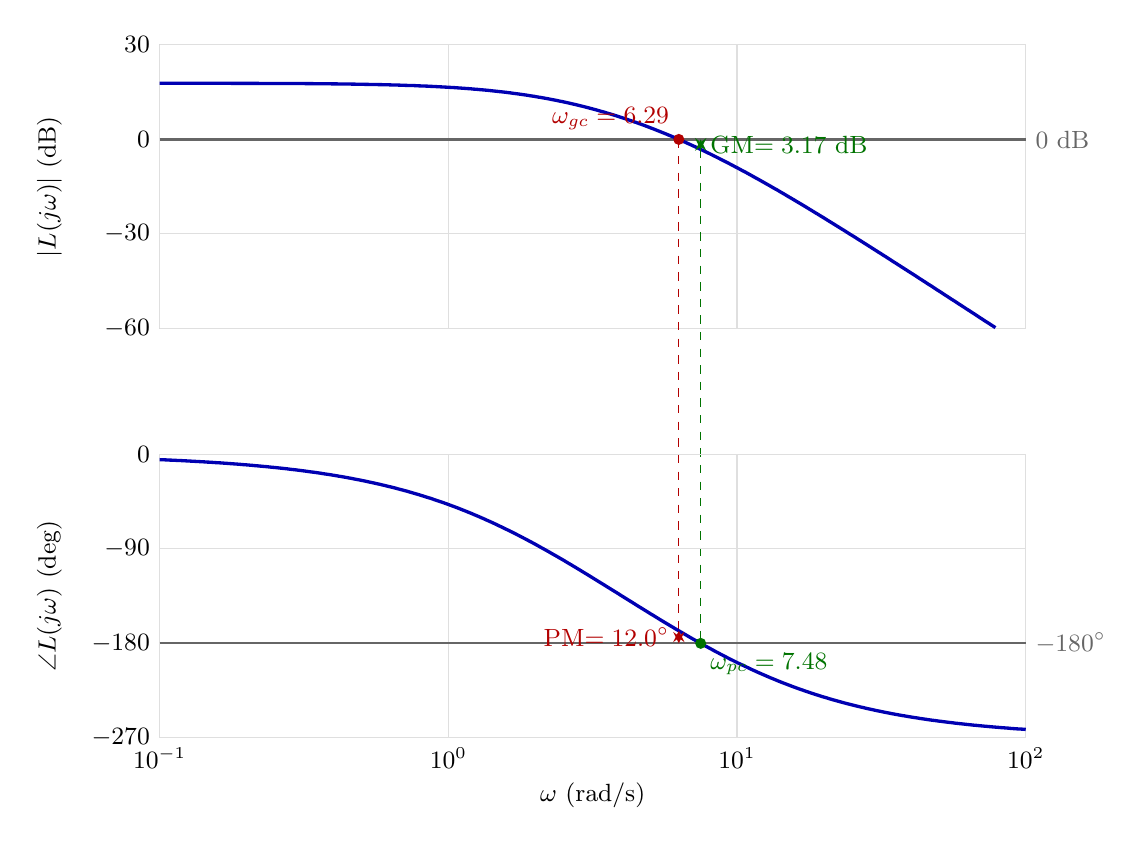
\begin{tikzpicture}[x=1cm,y=1cm,font=\small,>=stealth]
\draw[gray!30] (0,0) rectangle (11.0,3.6);
\draw[gray!25] (0,0.000)--(11.0,0.000); \node[left] at (0,0.000) {$-60$};
\draw[gray!25] (0,1.200)--(11.0,1.200); \node[left] at (0,1.200) {$-30$};
\draw[gray!25] (0,2.400)--(11.0,2.400); \node[left] at (0,2.400) {$0$};
\draw[gray!25] (0,3.600)--(11.0,3.600); \node[left] at (0,3.600) {$30$};
\draw[gray!25] (0.000,0)--(0.000,3.6);
\draw[gray!25] (3.667,0)--(3.667,3.6);
\draw[gray!25] (7.333,0)--(7.333,3.6);
\draw[gray!25] (11.000,0)--(11.000,3.6);
\draw[black!60,thick] (0,2.400)--(11.0,2.400); \node[right,black!60] at (11.0,2.400) {0 dB};
\draw[blue!70!black,very thick] (0.000,3.114) -- (0.027,3.114) -- (0.055,3.114) -- (0.082,3.114) -- (0.110,3.114) -- (0.137,3.114) -- (0.165,3.114) -- (0.192,3.114) -- (0.220,3.113) -- (0.247,3.113) -- (0.275,3.113) -- (0.303,3.113) -- (0.330,3.113) -- (0.358,3.113) -- (0.385,3.113) -- (0.413,3.113) -- (0.440,3.113) -- (0.467,3.113) -- (0.495,3.113) -- (0.522,3.113) -- (0.550,3.113) -- (0.577,3.113) -- (0.605,3.113) -- (0.632,3.113) -- (0.660,3.113) -- (0.688,3.113) -- (0.715,3.113) -- (0.743,3.113) -- (0.770,3.113) -- (0.798,3.113) -- (0.825,3.113) -- (0.853,3.113) -- (0.880,3.113) -- (0.908,3.112) -- (0.935,3.112) -- (0.962,3.112) -- (0.990,3.112) -- (1.018,3.112) -- (1.045,3.112) -- (1.072,3.112) -- (1.100,3.112) -- (1.127,3.112) -- (1.155,3.112) -- (1.182,3.112) -- (1.210,3.112) -- (1.238,3.112) -- (1.265,3.111) -- (1.292,3.111) -- (1.320,3.111) -- (1.347,3.111) -- (1.375,3.111) -- (1.403,3.111) -- (1.430,3.111) -- (1.457,3.111) -- (1.485,3.111) -- (1.512,3.110) -- (1.540,3.110) -- (1.567,3.110) -- (1.595,3.110) -- (1.623,3.110) -- (1.650,3.110) -- (1.677,3.110) -- (1.705,3.109) -- (1.732,3.109) -- (1.760,3.109) -- (1.788,3.109) -- (1.815,3.109) -- (1.842,3.109) -- (1.870,3.108) -- (1.897,3.108) -- (1.925,3.108) -- (1.952,3.108) -- (1.980,3.107) -- (2.007,3.107) -- (2.035,3.107) -- (2.062,3.107) -- (2.090,3.106) -- (2.118,3.106) -- (2.145,3.106) -- (2.172,3.106) -- (2.200,3.105) -- (2.228,3.105) -- (2.255,3.105) -- (2.283,3.104) -- (2.310,3.104) -- (2.337,3.104) -- (2.365,3.103) -- (2.392,3.103) -- (2.420,3.103) -- (2.447,3.102) -- (2.475,3.102) -- (2.502,3.101) -- (2.530,3.101) -- (2.558,3.100) -- (2.585,3.100) -- (2.612,3.099) -- (2.640,3.099) -- (2.667,3.098) -- (2.695,3.098) -- (2.723,3.097) -- (2.750,3.097) -- (2.777,3.096) -- (2.805,3.096) -- (2.832,3.095) -- (2.860,3.094) -- (2.887,3.094) -- (2.915,3.093) -- (2.942,3.092) -- (2.970,3.091) -- (2.998,3.091) -- (3.025,3.090) -- (3.052,3.089) -- (3.080,3.088) -- (3.107,3.087) -- (3.135,3.086) -- (3.163,3.085) -- (3.190,3.085) -- (3.217,3.084) -- (3.245,3.083) -- (3.272,3.081) -- (3.300,3.080) -- (3.327,3.079) -- (3.355,3.078) -- (3.382,3.077) -- (3.410,3.076) -- (3.438,3.074) -- (3.465,3.073) -- (3.492,3.072) -- (3.520,3.070) -- (3.547,3.069) -- (3.575,3.067) -- (3.603,3.066) -- (3.630,3.064) -- (3.658,3.063) -- (3.685,3.061) -- (3.712,3.059) -- (3.740,3.058) -- (3.768,3.056) -- (3.795,3.054) -- (3.822,3.052) -- (3.850,3.050) -- (3.878,3.048) -- (3.905,3.046) -- (3.932,3.044) -- (3.960,3.042) -- (3.987,3.039) -- (4.015,3.037) -- (4.042,3.035) -- (4.070,3.032) -- (4.097,3.030) -- (4.125,3.027) -- (4.152,3.025) -- (4.180,3.022) -- (4.207,3.019) -- (4.235,3.016) -- (4.263,3.013) -- (4.290,3.010) -- (4.317,3.007) -- (4.345,3.004) -- (4.372,3.001) -- (4.400,2.998) -- (4.428,2.994) -- (4.455,2.991) -- (4.482,2.987) -- (4.510,2.983) -- (4.537,2.980) -- (4.565,2.976) -- (4.592,2.972) -- (4.620,2.968) -- (4.647,2.964) -- (4.675,2.960) -- (4.702,2.955) -- (4.730,2.951) -- (4.758,2.947) -- (4.785,2.942) -- (4.812,2.937) -- (4.840,2.933) -- (4.867,2.928) -- (4.895,2.923) -- (4.923,2.918) -- (4.950,2.913) -- (4.977,2.907) -- (5.005,2.902) -- (5.032,2.897) -- (5.060,2.891) -- (5.087,2.885) -- (5.115,2.880) -- (5.143,2.874) -- (5.170,2.868) -- (5.197,2.862) -- (5.225,2.855) -- (5.253,2.849) -- (5.280,2.843) -- (5.308,2.836) -- (5.335,2.829) -- (5.362,2.823) -- (5.390,2.816) -- (5.417,2.809) -- (5.445,2.802) -- (5.472,2.794) -- (5.500,2.787) -- (5.527,2.780) -- (5.555,2.772) -- (5.582,2.764) -- (5.610,2.756) -- (5.638,2.749) -- (5.665,2.741) -- (5.692,2.732) -- (5.720,2.724) -- (5.747,2.716) -- (5.775,2.707) -- (5.803,2.699) -- (5.830,2.690) -- (5.857,2.681) -- (5.885,2.672) -- (5.912,2.663) -- (5.940,2.654) -- (5.967,2.644) -- (5.995,2.635) -- (6.022,2.625) -- (6.050,2.616) -- (6.077,2.606) -- (6.105,2.596) -- (6.133,2.586) -- (6.160,2.576) -- (6.188,2.565) -- (6.215,2.555) -- (6.242,2.544) -- (6.270,2.534) -- (6.297,2.523) -- (6.325,2.512) -- (6.352,2.501) -- (6.380,2.490) -- (6.407,2.479) -- (6.435,2.468) -- (6.462,2.456) -- (6.490,2.445) -- (6.518,2.433) -- (6.545,2.421) -- (6.572,2.409) -- (6.600,2.397) -- (6.628,2.385) -- (6.655,2.373) -- (6.683,2.361) -- (6.710,2.348) -- (6.737,2.336) -- (6.765,2.323) -- (6.792,2.311) -- (6.820,2.298) -- (6.847,2.285) -- (6.875,2.272) -- (6.902,2.259) -- (6.930,2.245) -- (6.957,2.232) -- (6.985,2.219) -- (7.013,2.205) -- (7.040,2.191) -- (7.067,2.178) -- (7.095,2.164) -- (7.122,2.150) -- (7.150,2.136) -- (7.178,2.122) -- (7.205,2.108) -- (7.232,2.094) -- (7.260,2.079) -- (7.287,2.065) -- (7.315,2.050) -- (7.342,2.036) -- (7.370,2.021) -- (7.397,2.006) -- (7.425,1.992) -- (7.453,1.977) -- (7.480,1.962) -- (7.507,1.947) -- (7.535,1.931) -- (7.562,1.916) -- (7.590,1.901) -- (7.617,1.886) -- (7.645,1.870) -- (7.672,1.855) -- (7.700,1.839) -- (7.727,1.824) -- (7.755,1.808) -- (7.782,1.792) -- (7.810,1.776) -- (7.838,1.761) -- (7.865,1.745) -- (7.892,1.729) -- (7.920,1.713) -- (7.947,1.697) -- (7.975,1.680) -- (8.002,1.664) -- (8.030,1.648) -- (8.057,1.632) -- (8.085,1.615) -- (8.112,1.599) -- (8.140,1.583) -- (8.168,1.566) -- (8.195,1.550) -- (8.223,1.533) -- (8.250,1.516) -- (8.277,1.500) -- (8.305,1.483) -- (8.332,1.466) -- (8.360,1.450) -- (8.387,1.433) -- (8.415,1.416) -- (8.443,1.399) -- (8.470,1.382) -- (8.497,1.365) -- (8.525,1.348) -- (8.553,1.331) -- (8.580,1.314) -- (8.607,1.297) -- (8.635,1.280) -- (8.662,1.263) -- (8.690,1.246) -- (8.717,1.229) -- (8.745,1.211) -- (8.772,1.194) -- (8.800,1.177) -- (8.828,1.160) -- (8.855,1.142) -- (8.882,1.125) -- (8.910,1.108) -- (8.938,1.090) -- (8.965,1.073) -- (8.992,1.056) -- (9.020,1.038) -- (9.047,1.021) -- (9.075,1.003) -- (9.102,0.986) -- (9.130,0.968) -- (9.158,0.951) -- (9.185,0.933) -- (9.213,0.916) -- (9.240,0.898) -- (9.267,0.881) -- (9.295,0.863) -- (9.322,0.845) -- (9.350,0.828) -- (9.377,0.810) -- (9.405,0.793) -- (9.432,0.775) -- (9.460,0.757) -- (9.487,0.740) -- (9.515,0.722) -- (9.543,0.704) -- (9.570,0.687) -- (9.598,0.669) -- (9.625,0.651) -- (9.652,0.633) -- (9.680,0.616) -- (9.707,0.598) -- (9.735,0.580) -- (9.762,0.562) -- (9.790,0.545) -- (9.818,0.527) -- (9.845,0.509) -- (9.872,0.491) -- (9.900,0.473) -- (9.928,0.456) -- (9.955,0.438) -- (9.982,0.420) -- (10.010,0.402) -- (10.037,0.384) -- (10.065,0.366) -- (10.092,0.349) -- (10.120,0.331) -- (10.147,0.313) -- (10.175,0.295) -- (10.203,0.277) -- (10.230,0.259) -- (10.257,0.241) -- (10.285,0.224) -- (10.312,0.206) -- (10.340,0.188) -- (10.367,0.170) -- (10.395,0.152) -- (10.422,0.134) -- (10.450,0.116) -- (10.477,0.098) -- (10.505,0.080) -- (10.533,0.063) -- (10.560,0.045) -- (10.588,0.027) -- (10.615,0.009);
\node[rotate=90] at (-1.4,1.8) {$|L(j\omega)|$ (dB)};
\draw[red!70!black,dashed] (6.594,2.400)--(6.594,-3.840);
\fill[red!70!black] (6.594,2.400) circle(2pt); \node[above left,red!70!black] at (6.594,2.400) {$\omega_{gc}=6.29$};
\draw[green!45!black,dashed] (6.872,2.273)--(6.872,-4.000);
\draw[green!45!black,<->,thick] (6.872,2.273)--(6.872,2.400); \node[green!45!black,right] at (6.872,2.337) {GM$=3.17$ dB};
\draw[gray!30] (0,-5.2) rectangle (11.0,-1.6);
\draw[gray!25] (0,-5.200)--(11.0,-5.200); \node[left] at (0,-5.200) {$-270$};
\draw[gray!25] (0,-4.000)--(11.0,-4.000); \node[left] at (0,-4.000) {$-180$};
\draw[gray!25] (0,-2.800)--(11.0,-2.800); \node[left] at (0,-2.800) {$-90$};
\draw[gray!25] (0,-1.600)--(11.0,-1.600); \node[left] at (0,-1.600) {$0$};
\draw[gray!25] (0.000,-5.2)--(0.000,-1.6); \node[below] at (0.000,-5.2) {$10^{-1}$};
\draw[gray!25] (3.667,-5.2)--(3.667,-1.6); \node[below] at (3.667,-5.2) {$10^{0}$};
\draw[gray!25] (7.333,-5.2)--(7.333,-1.6); \node[below] at (7.333,-5.2) {$10^{1}$};
\draw[gray!25] (11.000,-5.2)--(11.000,-1.6); \node[below] at (11.000,-5.2) {$10^{2}$};
\draw[black!60,thick] (0,-4.000)--(11.0,-4.000); \node[right,black!60] at (11.0,-4.000) {$-180^\circ$};
\draw[blue!70!black,very thick] (0.000,-1.667) -- (0.027,-1.668) -- (0.055,-1.669) -- (0.082,-1.670) -- (0.110,-1.672) -- (0.137,-1.673) -- (0.165,-1.674) -- (0.192,-1.675) -- (0.220,-1.677) -- (0.247,-1.678) -- (0.275,-1.679) -- (0.303,-1.681) -- (0.330,-1.682) -- (0.358,-1.684) -- (0.385,-1.685) -- (0.413,-1.687) -- (0.440,-1.688) -- (0.467,-1.690) -- (0.495,-1.691) -- (0.522,-1.693) -- (0.550,-1.694) -- (0.577,-1.696) -- (0.605,-1.698) -- (0.632,-1.699) -- (0.660,-1.701) -- (0.688,-1.703) -- (0.715,-1.705) -- (0.743,-1.706) -- (0.770,-1.708) -- (0.798,-1.710) -- (0.825,-1.712) -- (0.853,-1.714) -- (0.880,-1.716) -- (0.908,-1.718) -- (0.935,-1.720) -- (0.962,-1.722) -- (0.990,-1.724) -- (1.018,-1.726) -- (1.045,-1.729) -- (1.072,-1.731) -- (1.100,-1.733) -- (1.127,-1.735) -- (1.155,-1.738) -- (1.182,-1.740) -- (1.210,-1.743) -- (1.238,-1.745) -- (1.265,-1.748) -- (1.292,-1.750) -- (1.320,-1.753) -- (1.347,-1.755) -- (1.375,-1.758) -- (1.403,-1.761) -- (1.430,-1.764) -- (1.457,-1.766) -- (1.485,-1.769) -- (1.512,-1.772) -- (1.540,-1.775) -- (1.567,-1.778) -- (1.595,-1.781) -- (1.623,-1.784) -- (1.650,-1.788) -- (1.677,-1.791) -- (1.705,-1.794) -- (1.732,-1.797) -- (1.760,-1.801) -- (1.788,-1.804) -- (1.815,-1.808) -- (1.842,-1.811) -- (1.870,-1.815) -- (1.897,-1.819) -- (1.925,-1.823) -- (1.952,-1.826) -- (1.980,-1.830) -- (2.007,-1.834) -- (2.035,-1.838) -- (2.062,-1.842) -- (2.090,-1.847) -- (2.118,-1.851) -- (2.145,-1.855) -- (2.172,-1.859) -- (2.200,-1.864) -- (2.228,-1.868) -- (2.255,-1.873) -- (2.283,-1.878) -- (2.310,-1.882) -- (2.337,-1.887) -- (2.365,-1.892) -- (2.392,-1.897) -- (2.420,-1.902) -- (2.447,-1.907) -- (2.475,-1.913) -- (2.502,-1.918) -- (2.530,-1.923) -- (2.558,-1.929) -- (2.585,-1.934) -- (2.612,-1.940) -- (2.640,-1.946) -- (2.667,-1.952) -- (2.695,-1.958) -- (2.723,-1.964) -- (2.750,-1.970) -- (2.777,-1.976) -- (2.805,-1.982) -- (2.832,-1.989) -- (2.860,-1.995) -- (2.887,-2.002) -- (2.915,-2.009) -- (2.942,-2.015) -- (2.970,-2.022) -- (2.998,-2.029) -- (3.025,-2.037) -- (3.052,-2.044) -- (3.080,-2.051) -- (3.107,-2.059) -- (3.135,-2.066) -- (3.163,-2.074) -- (3.190,-2.082) -- (3.217,-2.090) -- (3.245,-2.098) -- (3.272,-2.106) -- (3.300,-2.114) -- (3.327,-2.123) -- (3.355,-2.131) -- (3.382,-2.140) -- (3.410,-2.149) -- (3.438,-2.157) -- (3.465,-2.166) -- (3.492,-2.176) -- (3.520,-2.185) -- (3.547,-2.194) -- (3.575,-2.204) -- (3.603,-2.213) -- (3.630,-2.223) -- (3.658,-2.233) -- (3.685,-2.243) -- (3.712,-2.253) -- (3.740,-2.263) -- (3.768,-2.274) -- (3.795,-2.284) -- (3.822,-2.295) -- (3.850,-2.306) -- (3.878,-2.317) -- (3.905,-2.328) -- (3.932,-2.339) -- (3.960,-2.350) -- (3.987,-2.362) -- (4.015,-2.374) -- (4.042,-2.385) -- (4.070,-2.397) -- (4.097,-2.409) -- (4.125,-2.421) -- (4.152,-2.434) -- (4.180,-2.446) -- (4.207,-2.458) -- (4.235,-2.471) -- (4.263,-2.484) -- (4.290,-2.497) -- (4.317,-2.510) -- (4.345,-2.523) -- (4.372,-2.536) -- (4.400,-2.550) -- (4.428,-2.563) -- (4.455,-2.577) -- (4.482,-2.590) -- (4.510,-2.604) -- (4.537,-2.618) -- (4.565,-2.632) -- (4.592,-2.647) -- (4.620,-2.661) -- (4.647,-2.675) -- (4.675,-2.690) -- (4.702,-2.705) -- (4.730,-2.719) -- (4.758,-2.734) -- (4.785,-2.749) -- (4.812,-2.764) -- (4.840,-2.780) -- (4.867,-2.795) -- (4.895,-2.810) -- (4.923,-2.826) -- (4.950,-2.841) -- (4.977,-2.857) -- (5.005,-2.873) -- (5.032,-2.888) -- (5.060,-2.904) -- (5.087,-2.920) -- (5.115,-2.936) -- (5.143,-2.952) -- (5.170,-2.969) -- (5.197,-2.985) -- (5.225,-3.001) -- (5.253,-3.018) -- (5.280,-3.034) -- (5.308,-3.051) -- (5.335,-3.067) -- (5.362,-3.084) -- (5.390,-3.101) -- (5.417,-3.117) -- (5.445,-3.134) -- (5.472,-3.151) -- (5.500,-3.168) -- (5.527,-3.185) -- (5.555,-3.202) -- (5.582,-3.219) -- (5.610,-3.236) -- (5.638,-3.253) -- (5.665,-3.270) -- (5.692,-3.287) -- (5.720,-3.304) -- (5.747,-3.321) -- (5.775,-3.338) -- (5.803,-3.355) -- (5.830,-3.372) -- (5.857,-3.390) -- (5.885,-3.407) -- (5.912,-3.424) -- (5.940,-3.441) -- (5.967,-3.458) -- (5.995,-3.475) -- (6.022,-3.492) -- (6.050,-3.510) -- (6.077,-3.527) -- (6.105,-3.544) -- (6.133,-3.561) -- (6.160,-3.578) -- (6.188,-3.595) -- (6.215,-3.612) -- (6.242,-3.629) -- (6.270,-3.645) -- (6.297,-3.662) -- (6.325,-3.679) -- (6.352,-3.696) -- (6.380,-3.713) -- (6.407,-3.729) -- (6.435,-3.746) -- (6.462,-3.762) -- (6.490,-3.779) -- (6.518,-3.795) -- (6.545,-3.812) -- (6.572,-3.828) -- (6.600,-3.844) -- (6.628,-3.860) -- (6.655,-3.876) -- (6.683,-3.892) -- (6.710,-3.908) -- (6.737,-3.924) -- (6.765,-3.940) -- (6.792,-3.955) -- (6.820,-3.971) -- (6.847,-3.986) -- (6.875,-4.002) -- (6.902,-4.017) -- (6.930,-4.032) -- (6.957,-4.047) -- (6.985,-4.062) -- (7.013,-4.077) -- (7.040,-4.092) -- (7.067,-4.107) -- (7.095,-4.121) -- (7.122,-4.136) -- (7.150,-4.150) -- (7.178,-4.165) -- (7.205,-4.179) -- (7.232,-4.193) -- (7.260,-4.207) -- (7.287,-4.220) -- (7.315,-4.234) -- (7.342,-4.248) -- (7.370,-4.261) -- (7.397,-4.274) -- (7.425,-4.287) -- (7.453,-4.300) -- (7.480,-4.313) -- (7.507,-4.326) -- (7.535,-4.339) -- (7.562,-4.351) -- (7.590,-4.364) -- (7.617,-4.376) -- (7.645,-4.388) -- (7.672,-4.400) -- (7.700,-4.412) -- (7.727,-4.424) -- (7.755,-4.436) -- (7.782,-4.447) -- (7.810,-4.458) -- (7.838,-4.470) -- (7.865,-4.481) -- (7.892,-4.492) -- (7.920,-4.503) -- (7.947,-4.513) -- (7.975,-4.524) -- (8.002,-4.534) -- (8.030,-4.545) -- (8.057,-4.555) -- (8.085,-4.565) -- (8.112,-4.575) -- (8.140,-4.585) -- (8.168,-4.594) -- (8.195,-4.604) -- (8.223,-4.613) -- (8.250,-4.622) -- (8.277,-4.632) -- (8.305,-4.641) -- (8.332,-4.650) -- (8.360,-4.658) -- (8.387,-4.667) -- (8.415,-4.676) -- (8.443,-4.684) -- (8.470,-4.692) -- (8.497,-4.701) -- (8.525,-4.709) -- (8.553,-4.717) -- (8.580,-4.724) -- (8.607,-4.732) -- (8.635,-4.740) -- (8.662,-4.747) -- (8.690,-4.755) -- (8.717,-4.762) -- (8.745,-4.769) -- (8.772,-4.776) -- (8.800,-4.783) -- (8.828,-4.790) -- (8.855,-4.797) -- (8.882,-4.803) -- (8.910,-4.810) -- (8.938,-4.816) -- (8.965,-4.823) -- (8.992,-4.829) -- (9.020,-4.835) -- (9.047,-4.841) -- (9.075,-4.847) -- (9.102,-4.853) -- (9.130,-4.859) -- (9.158,-4.864) -- (9.185,-4.870) -- (9.213,-4.876) -- (9.240,-4.881) -- (9.267,-4.886) -- (9.295,-4.892) -- (9.322,-4.897) -- (9.350,-4.902) -- (9.377,-4.907) -- (9.405,-4.912) -- (9.432,-4.917) -- (9.460,-4.921) -- (9.487,-4.926) -- (9.515,-4.931) -- (9.543,-4.935) -- (9.570,-4.940) -- (9.598,-4.944) -- (9.625,-4.948) -- (9.652,-4.953) -- (9.680,-4.957) -- (9.707,-4.961) -- (9.735,-4.965) -- (9.762,-4.969) -- (9.790,-4.973) -- (9.818,-4.977) -- (9.845,-4.980) -- (9.872,-4.984) -- (9.900,-4.988) -- (9.928,-4.991) -- (9.955,-4.995) -- (9.982,-4.998) -- (10.010,-5.002) -- (10.037,-5.005) -- (10.065,-5.008) -- (10.092,-5.012) -- (10.120,-5.015) -- (10.147,-5.018) -- (10.175,-5.021) -- (10.203,-5.024) -- (10.230,-5.027) -- (10.257,-5.030) -- (10.285,-5.033) -- (10.312,-5.036) -- (10.340,-5.039) -- (10.367,-5.041) -- (10.395,-5.044) -- (10.422,-5.047) -- (10.450,-5.049) -- (10.477,-5.052) -- (10.505,-5.054) -- (10.533,-5.057) -- (10.560,-5.059) -- (10.588,-5.062) -- (10.615,-5.064) -- (10.642,-5.066) -- (10.670,-5.069) -- (10.697,-5.071) -- (10.725,-5.073) -- (10.752,-5.075) -- (10.780,-5.077) -- (10.807,-5.080) -- (10.835,-5.082) -- (10.862,-5.084) -- (10.890,-5.086) -- (10.918,-5.088) -- (10.945,-5.089) -- (10.973,-5.091) -- (11.000,-5.093);
\node[rotate=90] at (-1.4,-3.4000000000000004) {$\angle L(j\omega)$ (deg)};
\node[below=0.45cm] at (5.5,-5.2) {$\omega$ (rad/s)};
\draw[red!70!black,<->,thick] (6.594,-3.840)--(6.594,-4.000); \node[red!70!black,left] at (6.594,-3.920) {PM$=12.0^\circ$};
\fill[green!45!black] (6.872,-4.000) circle(2pt); \node[below right,green!45!black] at (6.872,-4.000) {$\omega_{pc}=7.48$};
\end{tikzpicture}
\caption{Bode ของตัวอย่าง 1: จุด $\omega_{gc}=6.29$ ให้ PM $\approx12^\circ$ และจุด $\omega_{pc}=7.48$ ให้ GM $\approx3.17$ dB}
\end{figure}

\paragraph{ตีความและตรวจคำตอบ}
GM และ PM เป็นบวกทั้งคู่ ระบบเสถียร แต่ทั้งสองค่าน้อยมาก (PM เพียง $12^\circ$) ผลตอบสนองจะแกว่งมากและไวต่อการเปลี่ยนแปลงของระบบ ตรวจด้วย Routh: ตัวส่วน $=s^3+14s^2+56s+64$ ระบบวงปิดคงเสถียรเมื่อ $14\cdot56>64+K$ คือ $K<720$ ส่วนกลับของ $|G(j\omega_{pc})|$ คือ $1/0.694=1.44$ และ $500\times1.44=720$ ตรงกับขอบเสถียรภาพพอดี แปลว่า GM $=20\log_{10}(720/500)=3.17$ dB ถูกต้อง

%=====================================================================
\section{ตัวอย่าง 2: ออกแบบ $K$ จาก PM}
\begin{exbox}{โจทย์}
ระบบวงปิดแบบ negative unity feedback มีตัวควบคุมสัดส่วน $K$ และพลานต์
\[
G(s)=\frac{100}{(s+2)(s+3)(s+4)}.
\]
(ก) หา $K$ ที่ทำให้ PM $\ge60^\circ$ \quad (ข) หา GM ที่ $K$ นั้น
\end{exbox}

\paragraph{ขั้น 1: Loop gain}
\[
L(\jw)=\frac{100K}{(\jw+2)(\jw+3)(\jw+4)},\quad
|L|=\frac{100K}{\sqrt{\omega^2+4}\sqrt{\omega^2+9}\sqrt{\omega^2+16}},
\]
\[
\angle L=-\Big(\atan\tfrac{\omega}{2}+\atan\tfrac{\omega}{3}+\atan\tfrac{\omega}{4}\Big).
\]

\paragraph{ขั้น 2 (ก): หาความถี่ที่เฟสเป็น $-120^\circ$}
PM $=60^\circ$ ต้องการ $\angle L(j\omega_{gc})=-180^\circ+60^\circ=-120^\circ$ จึงแก้
\[
\atan\tfrac{\omega}{2}+\atan\tfrac{\omega}{3}+\atan\tfrac{\omega}{4}=120^\circ
\ \Rightarrow\ \omega_{gc}\approx2.4\ \text{rad/s}.
\]
(ค่าละเอียดคือ $2.405$)

\paragraph{ขั้น 3 (ก): บังคับ $|L|=1$ ที่ความถี่นั้น}
\[
\frac{100K}{\sqrt{2.4^2+4}\sqrt{2.4^2+9}\sqrt{2.4^2+16}}=1
\ \Rightarrow\ \boxed{K\approx0.56}
\]
(ค่าละเอียด $K=0.5614$)

\paragraph{ขั้น 4 (ข): GM ที่ $K=0.56$}
เฟสไม่ขึ้นกับ $K$ จึงหา $\omega_{pc}$ จาก $\sum\atan(\omega/a_i)=180^\circ$ ได้ $\omega_{pc}\approx5.1$ rad/s (ทางลัด: $\omega_{pc}^2=2\cdot3+2\cdot4+3\cdot4=26\Rightarrow\sqrt{26}=5.099$) แทนใน $|L|$ โดย $100K=56$:
\[
|L(j\omega_{pc})|=\frac{56}{\sqrt{5.1^2+4}\sqrt{5.1^2+9}\sqrt{5.1^2+16}}\approx0.267
\ \Rightarrow\ 20\log_{10}(0.267)=-11.5\dB
\]
\[
\boxed{\mathrm{GM}\approx11.5\dB}
\]

\begin{figure}[h]
\centering
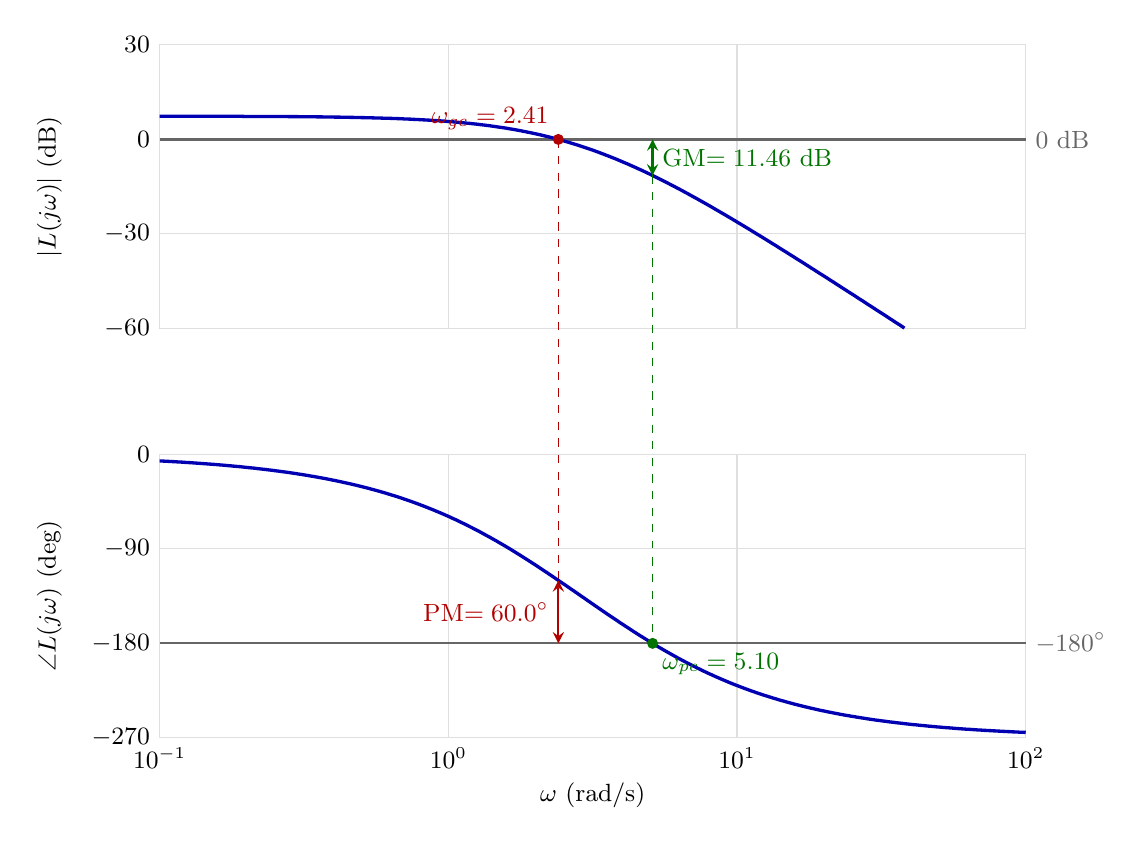
\begin{tikzpicture}[x=1cm,y=1cm,font=\small,>=stealth]
\draw[gray!30] (0,0) rectangle (11.0,3.6);
\draw[gray!25] (0,0.000)--(11.0,0.000); \node[left] at (0,0.000) {$-60$};
\draw[gray!25] (0,1.200)--(11.0,1.200); \node[left] at (0,1.200) {$-30$};
\draw[gray!25] (0,2.400)--(11.0,2.400); \node[left] at (0,2.400) {$0$};
\draw[gray!25] (0,3.600)--(11.0,3.600); \node[left] at (0,3.600) {$30$};
\draw[gray!25] (0.000,0)--(0.000,3.6);
\draw[gray!25] (3.667,0)--(3.667,3.6);
\draw[gray!25] (7.333,0)--(7.333,3.6);
\draw[gray!25] (11.000,0)--(11.000,3.6);
\draw[black!60,thick] (0,2.400)--(11.0,2.400); \node[right,black!60] at (11.0,2.400) {0 dB};
\draw[blue!70!black,very thick] (0.000,2.695) -- (0.027,2.695) -- (0.055,2.694) -- (0.082,2.694) -- (0.110,2.694) -- (0.137,2.694) -- (0.165,2.694) -- (0.192,2.694) -- (0.220,2.694) -- (0.247,2.694) -- (0.275,2.694) -- (0.303,2.694) -- (0.330,2.694) -- (0.358,2.694) -- (0.385,2.694) -- (0.413,2.694) -- (0.440,2.694) -- (0.467,2.694) -- (0.495,2.694) -- (0.522,2.694) -- (0.550,2.694) -- (0.577,2.694) -- (0.605,2.694) -- (0.632,2.694) -- (0.660,2.694) -- (0.688,2.694) -- (0.715,2.693) -- (0.743,2.693) -- (0.770,2.693) -- (0.798,2.693) -- (0.825,2.693) -- (0.853,2.693) -- (0.880,2.693) -- (0.908,2.693) -- (0.935,2.693) -- (0.962,2.693) -- (0.990,2.693) -- (1.018,2.693) -- (1.045,2.693) -- (1.072,2.692) -- (1.100,2.692) -- (1.127,2.692) -- (1.155,2.692) -- (1.182,2.692) -- (1.210,2.692) -- (1.238,2.692) -- (1.265,2.692) -- (1.292,2.692) -- (1.320,2.691) -- (1.347,2.691) -- (1.375,2.691) -- (1.403,2.691) -- (1.430,2.691) -- (1.457,2.691) -- (1.485,2.691) -- (1.512,2.690) -- (1.540,2.690) -- (1.567,2.690) -- (1.595,2.690) -- (1.623,2.690) -- (1.650,2.689) -- (1.677,2.689) -- (1.705,2.689) -- (1.732,2.689) -- (1.760,2.689) -- (1.788,2.688) -- (1.815,2.688) -- (1.842,2.688) -- (1.870,2.688) -- (1.897,2.687) -- (1.925,2.687) -- (1.952,2.687) -- (1.980,2.687) -- (2.007,2.686) -- (2.035,2.686) -- (2.062,2.686) -- (2.090,2.685) -- (2.118,2.685) -- (2.145,2.685) -- (2.172,2.684) -- (2.200,2.684) -- (2.228,2.683) -- (2.255,2.683) -- (2.283,2.683) -- (2.310,2.682) -- (2.337,2.682) -- (2.365,2.681) -- (2.392,2.681) -- (2.420,2.680) -- (2.447,2.680) -- (2.475,2.679) -- (2.502,2.679) -- (2.530,2.678) -- (2.558,2.677) -- (2.585,2.677) -- (2.612,2.676) -- (2.640,2.676) -- (2.667,2.675) -- (2.695,2.674) -- (2.723,2.673) -- (2.750,2.673) -- (2.777,2.672) -- (2.805,2.671) -- (2.832,2.670) -- (2.860,2.669) -- (2.887,2.669) -- (2.915,2.668) -- (2.942,2.667) -- (2.970,2.666) -- (2.998,2.665) -- (3.025,2.664) -- (3.052,2.663) -- (3.080,2.662) -- (3.107,2.660) -- (3.135,2.659) -- (3.163,2.658) -- (3.190,2.657) -- (3.217,2.655) -- (3.245,2.654) -- (3.272,2.653) -- (3.300,2.651) -- (3.327,2.650) -- (3.355,2.648) -- (3.382,2.647) -- (3.410,2.645) -- (3.438,2.644) -- (3.465,2.642) -- (3.492,2.640) -- (3.520,2.638) -- (3.547,2.636) -- (3.575,2.635) -- (3.603,2.633) -- (3.630,2.630) -- (3.658,2.628) -- (3.685,2.626) -- (3.712,2.624) -- (3.740,2.622) -- (3.768,2.619) -- (3.795,2.617) -- (3.822,2.614) -- (3.850,2.612) -- (3.878,2.609) -- (3.905,2.606) -- (3.932,2.604) -- (3.960,2.601) -- (3.987,2.598) -- (4.015,2.595) -- (4.042,2.592) -- (4.070,2.588) -- (4.097,2.585) -- (4.125,2.582) -- (4.152,2.578) -- (4.180,2.575) -- (4.207,2.571) -- (4.235,2.567) -- (4.263,2.563) -- (4.290,2.559) -- (4.317,2.555) -- (4.345,2.551) -- (4.372,2.547) -- (4.400,2.543) -- (4.428,2.538) -- (4.455,2.533) -- (4.482,2.529) -- (4.510,2.524) -- (4.537,2.519) -- (4.565,2.514) -- (4.592,2.509) -- (4.620,2.503) -- (4.647,2.498) -- (4.675,2.492) -- (4.702,2.487) -- (4.730,2.481) -- (4.758,2.475) -- (4.785,2.469) -- (4.812,2.463) -- (4.840,2.457) -- (4.867,2.450) -- (4.895,2.443) -- (4.923,2.437) -- (4.950,2.430) -- (4.977,2.423) -- (5.005,2.416) -- (5.032,2.409) -- (5.060,2.401) -- (5.087,2.394) -- (5.115,2.386) -- (5.143,2.378) -- (5.170,2.370) -- (5.197,2.362) -- (5.225,2.354) -- (5.253,2.345) -- (5.280,2.337) -- (5.308,2.328) -- (5.335,2.319) -- (5.362,2.310) -- (5.390,2.301) -- (5.417,2.292) -- (5.445,2.283) -- (5.472,2.273) -- (5.500,2.264) -- (5.527,2.254) -- (5.555,2.244) -- (5.582,2.234) -- (5.610,2.223) -- (5.638,2.213) -- (5.665,2.202) -- (5.692,2.192) -- (5.720,2.181) -- (5.747,2.170) -- (5.775,2.159) -- (5.803,2.148) -- (5.830,2.136) -- (5.857,2.125) -- (5.885,2.113) -- (5.912,2.101) -- (5.940,2.090) -- (5.967,2.078) -- (5.995,2.065) -- (6.022,2.053) -- (6.050,2.041) -- (6.077,2.028) -- (6.105,2.016) -- (6.133,2.003) -- (6.160,1.990) -- (6.188,1.977) -- (6.215,1.964) -- (6.242,1.951) -- (6.270,1.937) -- (6.297,1.924) -- (6.325,1.910) -- (6.352,1.896) -- (6.380,1.883) -- (6.407,1.869) -- (6.435,1.855) -- (6.462,1.841) -- (6.490,1.826) -- (6.518,1.812) -- (6.545,1.798) -- (6.572,1.783) -- (6.600,1.769) -- (6.628,1.754) -- (6.655,1.739) -- (6.683,1.724) -- (6.710,1.710) -- (6.737,1.694) -- (6.765,1.679) -- (6.792,1.664) -- (6.820,1.649) -- (6.847,1.634) -- (6.875,1.618) -- (6.902,1.603) -- (6.930,1.587) -- (6.957,1.572) -- (6.985,1.556) -- (7.013,1.540) -- (7.040,1.524) -- (7.067,1.508) -- (7.095,1.492) -- (7.122,1.476) -- (7.150,1.460) -- (7.178,1.444) -- (7.205,1.428) -- (7.232,1.412) -- (7.260,1.396) -- (7.287,1.379) -- (7.315,1.363) -- (7.342,1.346) -- (7.370,1.330) -- (7.397,1.313) -- (7.425,1.297) -- (7.453,1.280) -- (7.480,1.264) -- (7.507,1.247) -- (7.535,1.230) -- (7.562,1.213) -- (7.590,1.196) -- (7.617,1.180) -- (7.645,1.163) -- (7.672,1.146) -- (7.700,1.129) -- (7.727,1.112) -- (7.755,1.095) -- (7.782,1.078) -- (7.810,1.061) -- (7.838,1.044) -- (7.865,1.026) -- (7.892,1.009) -- (7.920,0.992) -- (7.947,0.975) -- (7.975,0.958) -- (8.002,0.940) -- (8.030,0.923) -- (8.057,0.906) -- (8.085,0.888) -- (8.112,0.871) -- (8.140,0.854) -- (8.168,0.836) -- (8.195,0.819) -- (8.223,0.801) -- (8.250,0.784) -- (8.277,0.766) -- (8.305,0.749) -- (8.332,0.731) -- (8.360,0.714) -- (8.387,0.696) -- (8.415,0.679) -- (8.443,0.661) -- (8.470,0.644) -- (8.497,0.626) -- (8.525,0.608) -- (8.553,0.591) -- (8.580,0.573) -- (8.607,0.555) -- (8.635,0.538) -- (8.662,0.520) -- (8.690,0.502) -- (8.717,0.485) -- (8.745,0.467) -- (8.772,0.449) -- (8.800,0.432) -- (8.828,0.414) -- (8.855,0.396) -- (8.882,0.378) -- (8.910,0.361) -- (8.938,0.343) -- (8.965,0.325) -- (8.992,0.307) -- (9.020,0.289) -- (9.047,0.272) -- (9.075,0.254) -- (9.102,0.236) -- (9.130,0.218) -- (9.158,0.200) -- (9.185,0.183) -- (9.213,0.165) -- (9.240,0.147) -- (9.267,0.129) -- (9.295,0.111) -- (9.322,0.093) -- (9.350,0.075) -- (9.377,0.058) -- (9.405,0.040) -- (9.432,0.022) -- (9.460,0.004);
\node[rotate=90] at (-1.4,1.8) {$|L(j\omega)|$ (dB)};
\draw[red!70!black,dashed] (5.064,2.400)--(5.064,-3.200);
\fill[red!70!black] (5.064,2.400) circle(2pt); \node[above left,red!70!black] at (5.064,2.400) {$\omega_{gc}=2.41$};
\draw[green!45!black,dashed] (6.261,1.942)--(6.261,-4.000);
\draw[green!45!black,<->,thick] (6.261,1.942)--(6.261,2.400); \node[green!45!black,right] at (6.261,2.171) {GM$=11.46$ dB};
\draw[gray!30] (0,-5.2) rectangle (11.0,-1.6);
\draw[gray!25] (0,-5.200)--(11.0,-5.200); \node[left] at (0,-5.200) {$-270$};
\draw[gray!25] (0,-4.000)--(11.0,-4.000); \node[left] at (0,-4.000) {$-180$};
\draw[gray!25] (0,-2.800)--(11.0,-2.800); \node[left] at (0,-2.800) {$-90$};
\draw[gray!25] (0,-1.600)--(11.0,-1.600); \node[left] at (0,-1.600) {$0$};
\draw[gray!25] (0.000,-5.2)--(0.000,-1.6); \node[below] at (0.000,-5.2) {$10^{-1}$};
\draw[gray!25] (3.667,-5.2)--(3.667,-1.6); \node[below] at (3.667,-5.2) {$10^{0}$};
\draw[gray!25] (7.333,-5.2)--(7.333,-1.6); \node[below] at (7.333,-5.2) {$10^{1}$};
\draw[gray!25] (11.000,-5.2)--(11.000,-1.6); \node[below] at (11.000,-5.2) {$10^{2}$};
\draw[black!60,thick] (0,-4.000)--(11.0,-4.000); \node[right,black!60] at (11.0,-4.000) {$-180^\circ$};
\draw[blue!70!black,very thick] (0.000,-1.683) -- (0.027,-1.684) -- (0.055,-1.686) -- (0.082,-1.687) -- (0.110,-1.689) -- (0.137,-1.690) -- (0.165,-1.692) -- (0.192,-1.693) -- (0.220,-1.695) -- (0.247,-1.697) -- (0.275,-1.698) -- (0.303,-1.700) -- (0.330,-1.702) -- (0.358,-1.704) -- (0.385,-1.705) -- (0.413,-1.707) -- (0.440,-1.709) -- (0.467,-1.711) -- (0.495,-1.713) -- (0.522,-1.715) -- (0.550,-1.717) -- (0.577,-1.719) -- (0.605,-1.721) -- (0.632,-1.723) -- (0.660,-1.725) -- (0.688,-1.727) -- (0.715,-1.729) -- (0.743,-1.732) -- (0.770,-1.734) -- (0.798,-1.736) -- (0.825,-1.739) -- (0.853,-1.741) -- (0.880,-1.744) -- (0.908,-1.746) -- (0.935,-1.749) -- (0.962,-1.751) -- (0.990,-1.754) -- (1.018,-1.756) -- (1.045,-1.759) -- (1.072,-1.762) -- (1.100,-1.765) -- (1.127,-1.768) -- (1.155,-1.771) -- (1.182,-1.773) -- (1.210,-1.776) -- (1.238,-1.780) -- (1.265,-1.783) -- (1.292,-1.786) -- (1.320,-1.789) -- (1.347,-1.792) -- (1.375,-1.796) -- (1.403,-1.799) -- (1.430,-1.802) -- (1.457,-1.806) -- (1.485,-1.810) -- (1.512,-1.813) -- (1.540,-1.817) -- (1.567,-1.821) -- (1.595,-1.824) -- (1.623,-1.828) -- (1.650,-1.832) -- (1.677,-1.836) -- (1.705,-1.840) -- (1.732,-1.844) -- (1.760,-1.849) -- (1.788,-1.853) -- (1.815,-1.857) -- (1.842,-1.862) -- (1.870,-1.866) -- (1.897,-1.871) -- (1.925,-1.876) -- (1.952,-1.880) -- (1.980,-1.885) -- (2.007,-1.890) -- (2.035,-1.895) -- (2.062,-1.900) -- (2.090,-1.905) -- (2.118,-1.910) -- (2.145,-1.916) -- (2.172,-1.921) -- (2.200,-1.927) -- (2.228,-1.932) -- (2.255,-1.938) -- (2.283,-1.944) -- (2.310,-1.950) -- (2.337,-1.956) -- (2.365,-1.962) -- (2.392,-1.968) -- (2.420,-1.974) -- (2.447,-1.980) -- (2.475,-1.987) -- (2.502,-1.993) -- (2.530,-2.000) -- (2.558,-2.007) -- (2.585,-2.014) -- (2.612,-2.021) -- (2.640,-2.028) -- (2.667,-2.035) -- (2.695,-2.043) -- (2.723,-2.050) -- (2.750,-2.058) -- (2.777,-2.065) -- (2.805,-2.073) -- (2.832,-2.081) -- (2.860,-2.089) -- (2.887,-2.097) -- (2.915,-2.106) -- (2.942,-2.114) -- (2.970,-2.123) -- (2.998,-2.131) -- (3.025,-2.140) -- (3.052,-2.149) -- (3.080,-2.158) -- (3.107,-2.168) -- (3.135,-2.177) -- (3.163,-2.187) -- (3.190,-2.196) -- (3.217,-2.206) -- (3.245,-2.216) -- (3.272,-2.226) -- (3.300,-2.236) -- (3.327,-2.247) -- (3.355,-2.257) -- (3.382,-2.268) -- (3.410,-2.279) -- (3.438,-2.290) -- (3.465,-2.301) -- (3.492,-2.312) -- (3.520,-2.324) -- (3.547,-2.335) -- (3.575,-2.347) -- (3.603,-2.359) -- (3.630,-2.371) -- (3.658,-2.383) -- (3.685,-2.395) -- (3.712,-2.408) -- (3.740,-2.421) -- (3.768,-2.433) -- (3.795,-2.446) -- (3.822,-2.460) -- (3.850,-2.473) -- (3.878,-2.486) -- (3.905,-2.500) -- (3.932,-2.514) -- (3.960,-2.528) -- (3.987,-2.542) -- (4.015,-2.556) -- (4.042,-2.570) -- (4.070,-2.585) -- (4.097,-2.600) -- (4.125,-2.615) -- (4.152,-2.630) -- (4.180,-2.645) -- (4.207,-2.660) -- (4.235,-2.676) -- (4.263,-2.691) -- (4.290,-2.707) -- (4.317,-2.723) -- (4.345,-2.739) -- (4.372,-2.755) -- (4.400,-2.771) -- (4.428,-2.788) -- (4.455,-2.804) -- (4.482,-2.821) -- (4.510,-2.838) -- (4.537,-2.855) -- (4.565,-2.872) -- (4.592,-2.889) -- (4.620,-2.907) -- (4.647,-2.924) -- (4.675,-2.942) -- (4.702,-2.959) -- (4.730,-2.977) -- (4.758,-2.995) -- (4.785,-3.013) -- (4.812,-3.031) -- (4.840,-3.049) -- (4.867,-3.067) -- (4.895,-3.086) -- (4.923,-3.104) -- (4.950,-3.123) -- (4.977,-3.141) -- (5.005,-3.160) -- (5.032,-3.178) -- (5.060,-3.197) -- (5.087,-3.216) -- (5.115,-3.235) -- (5.143,-3.253) -- (5.170,-3.272) -- (5.197,-3.291) -- (5.225,-3.310) -- (5.253,-3.329) -- (5.280,-3.348) -- (5.308,-3.367) -- (5.335,-3.386) -- (5.362,-3.405) -- (5.390,-3.424) -- (5.417,-3.443) -- (5.445,-3.462) -- (5.472,-3.481) -- (5.500,-3.500) -- (5.527,-3.519) -- (5.555,-3.538) -- (5.582,-3.557) -- (5.610,-3.576) -- (5.638,-3.595) -- (5.665,-3.614) -- (5.692,-3.632) -- (5.720,-3.651) -- (5.747,-3.669) -- (5.775,-3.688) -- (5.803,-3.706) -- (5.830,-3.725) -- (5.857,-3.743) -- (5.885,-3.761) -- (5.912,-3.779) -- (5.940,-3.797) -- (5.967,-3.815) -- (5.995,-3.833) -- (6.022,-3.851) -- (6.050,-3.869) -- (6.077,-3.886) -- (6.105,-3.904) -- (6.133,-3.921) -- (6.160,-3.938) -- (6.188,-3.955) -- (6.215,-3.972) -- (6.242,-3.989) -- (6.270,-4.006) -- (6.297,-4.022) -- (6.325,-4.039) -- (6.352,-4.055) -- (6.380,-4.071) -- (6.407,-4.087) -- (6.435,-4.103) -- (6.462,-4.118) -- (6.490,-4.134) -- (6.518,-4.149) -- (6.545,-4.165) -- (6.572,-4.180) -- (6.600,-4.195) -- (6.628,-4.210) -- (6.655,-4.224) -- (6.683,-4.239) -- (6.710,-4.253) -- (6.737,-4.267) -- (6.765,-4.281) -- (6.792,-4.295) -- (6.820,-4.309) -- (6.847,-4.322) -- (6.875,-4.336) -- (6.902,-4.349) -- (6.930,-4.362) -- (6.957,-4.375) -- (6.985,-4.388) -- (7.013,-4.400) -- (7.040,-4.413) -- (7.067,-4.425) -- (7.095,-4.437) -- (7.122,-4.449) -- (7.150,-4.461) -- (7.178,-4.473) -- (7.205,-4.484) -- (7.232,-4.496) -- (7.260,-4.507) -- (7.287,-4.518) -- (7.315,-4.529) -- (7.342,-4.539) -- (7.370,-4.550) -- (7.397,-4.560) -- (7.425,-4.571) -- (7.453,-4.581) -- (7.480,-4.591) -- (7.507,-4.601) -- (7.535,-4.611) -- (7.562,-4.620) -- (7.590,-4.630) -- (7.617,-4.639) -- (7.645,-4.648) -- (7.672,-4.657) -- (7.700,-4.666) -- (7.727,-4.675) -- (7.755,-4.683) -- (7.782,-4.692) -- (7.810,-4.700) -- (7.838,-4.708) -- (7.865,-4.717) -- (7.892,-4.725) -- (7.920,-4.732) -- (7.947,-4.740) -- (7.975,-4.748) -- (8.002,-4.755) -- (8.030,-4.763) -- (8.057,-4.770) -- (8.085,-4.777) -- (8.112,-4.784) -- (8.140,-4.791) -- (8.168,-4.798) -- (8.195,-4.805) -- (8.223,-4.811) -- (8.250,-4.818) -- (8.277,-4.824) -- (8.305,-4.830) -- (8.332,-4.837) -- (8.360,-4.843) -- (8.387,-4.849) -- (8.415,-4.855) -- (8.443,-4.860) -- (8.470,-4.866) -- (8.497,-4.872) -- (8.525,-4.877) -- (8.553,-4.883) -- (8.580,-4.888) -- (8.607,-4.893) -- (8.635,-4.899) -- (8.662,-4.904) -- (8.690,-4.909) -- (8.717,-4.914) -- (8.745,-4.918) -- (8.772,-4.923) -- (8.800,-4.928) -- (8.828,-4.932) -- (8.855,-4.937) -- (8.882,-4.941) -- (8.910,-4.946) -- (8.938,-4.950) -- (8.965,-4.954) -- (8.992,-4.959) -- (9.020,-4.963) -- (9.047,-4.967) -- (9.075,-4.971) -- (9.102,-4.975) -- (9.130,-4.978) -- (9.158,-4.982) -- (9.185,-4.986) -- (9.213,-4.989) -- (9.240,-4.993) -- (9.267,-4.997) -- (9.295,-5.000) -- (9.322,-5.003) -- (9.350,-5.007) -- (9.377,-5.010) -- (9.405,-5.013) -- (9.432,-5.016) -- (9.460,-5.020) -- (9.487,-5.023) -- (9.515,-5.026) -- (9.543,-5.029) -- (9.570,-5.032) -- (9.598,-5.034) -- (9.625,-5.037) -- (9.652,-5.040) -- (9.680,-5.043) -- (9.707,-5.045) -- (9.735,-5.048) -- (9.762,-5.051) -- (9.790,-5.053) -- (9.818,-5.056) -- (9.845,-5.058) -- (9.872,-5.061) -- (9.900,-5.063) -- (9.928,-5.065) -- (9.955,-5.068) -- (9.982,-5.070) -- (10.010,-5.072) -- (10.037,-5.074) -- (10.065,-5.076) -- (10.092,-5.079) -- (10.120,-5.081) -- (10.147,-5.083) -- (10.175,-5.085) -- (10.203,-5.087) -- (10.230,-5.089) -- (10.257,-5.091) -- (10.285,-5.092) -- (10.312,-5.094) -- (10.340,-5.096) -- (10.367,-5.098) -- (10.395,-5.100) -- (10.422,-5.101) -- (10.450,-5.103) -- (10.477,-5.105) -- (10.505,-5.106) -- (10.533,-5.108) -- (10.560,-5.109) -- (10.588,-5.111) -- (10.615,-5.112) -- (10.642,-5.114) -- (10.670,-5.115) -- (10.697,-5.117) -- (10.725,-5.118) -- (10.752,-5.120) -- (10.780,-5.121) -- (10.807,-5.122) -- (10.835,-5.124) -- (10.862,-5.125) -- (10.890,-5.126) -- (10.918,-5.128) -- (10.945,-5.129) -- (10.973,-5.130) -- (11.000,-5.131);
\node[rotate=90] at (-1.4,-3.4000000000000004) {$\angle L(j\omega)$ (deg)};
\node[below=0.45cm] at (5.5,-5.2) {$\omega$ (rad/s)};
\draw[red!70!black,<->,thick] (5.064,-3.200)--(5.064,-4.000); \node[red!70!black,left] at (5.064,-3.600) {PM$=60.0^\circ$};
\fill[green!45!black] (6.261,-4.000) circle(2pt); \node[below right,green!45!black] at (6.261,-4.000) {$\omega_{pc}=5.10$};
\end{tikzpicture}
\caption{Bode ของตัวอย่าง 2 ที่ $K=0.5614$: PM $=60^\circ$ ที่ $\omega_{gc}=2.41$ และ GM $\approx11.5$ dB ที่ $\omega_{pc}=5.10$}
\end{figure}

\paragraph{ตรวจคำตอบด้วย Routh}
ตัวส่วน $=s^3+9s^2+26s+24$ เสถียรเมื่อ $9\cdot26>24+100K$ คือ $K<2.1$ ดังนั้น GM $=20\log_{10}(2.1/0.5614)=11.5$ dB ตรงกับผลข้างต้น

%=====================================================================
\section{ตัวอย่าง 3: ออกแบบ $K$ จาก GM (ระบบอันดับ 4 มี zero)}
\begin{exbox}{โจทย์}
ระบบวงปิด unity feedback ตัวควบคุมสัดส่วน $K$ พลานต์
\[
G(s)=\frac{100(s+2)}{(s+1)(s+4)(s+5)(s+6)}.
\]
(ก) หา $K$ ที่ทำให้ GM $\ge12$ dB \quad (ข) หา PM ที่ $K$ นั้น
\end{exbox}

\paragraph{ขั้น 1: Loop gain}
ตัวเศษ $(\jw+2)$ ให้เฟส \emph{บวก} ตัวส่วนสี่ตัวให้เฟสลบ:
\[
|L|=\frac{100K\sqrt{\omega^2+4}}{\sqrt{\omega^2+1}\sqrt{\omega^2+16}\sqrt{\omega^2+25}\sqrt{\omega^2+36}},
\]
\[
\angle L=\atan\tfrac{\omega}{2}-\atan\omega-\atan\tfrac{\omega}{4}-\atan\tfrac{\omega}{5}-\atan\tfrac{\omega}{6}.
\]

\paragraph{ขั้น 2 (ก): GM $\ge12$ dB หมายถึง $|L(j\omega_{pc})|=10^{-12/20}$}
\[
|L(j\omega_{pc})|=10^{-12/20}\approx0.251.
\]
เฟสเป็น $-180^\circ$ ที่ $\omega_{pc}\approx7.83$ rad/s (ไม่ขึ้นกับ $K$ ตัวเศษทำให้ทางลัดใช้ไม่ได้ ต้องใช้ solver) แทนในสูตรขนาด:
\[
\frac{100K\sqrt{7.83^2+4}}{\sqrt{7.83^2+1}\sqrt{7.83^2+16}\sqrt{7.83^2+25}\sqrt{7.83^2+36}}=0.251
\ \Rightarrow\ \boxed{K\approx1.98}
\]
ค่านี้คือ \textbf{ค่าสูงสุด} ของ $K$ ที่ยังได้ GM ครบ 12 dB (เพิ่ม $K$ margin ลด ลด $K$ margin เพิ่ม) ถ้าต้องการความปลอดภัยเผื่อ เลือก $K$ ต่ำกว่านี้ เช่น $1.7$ หรือ $1.9$ ได้ ซึ่งเป็นการตัดสินใจเชิงออกแบบ

\paragraph{ขั้น 3 (ข): หา PM ที่ $K=1.98$}
ตั้ง $|L(\jw)|=1$ โดย $100K=198$ ได้ $\omega_{gc}\approx3.42$ rad/s แทนในเฟส ได้ $\angle L\approx-119^\circ$
\[
\boxed{\mathrm{PM}=180^\circ-119^\circ\approx61^\circ}
\]

\begin{figure}[h]
\centering
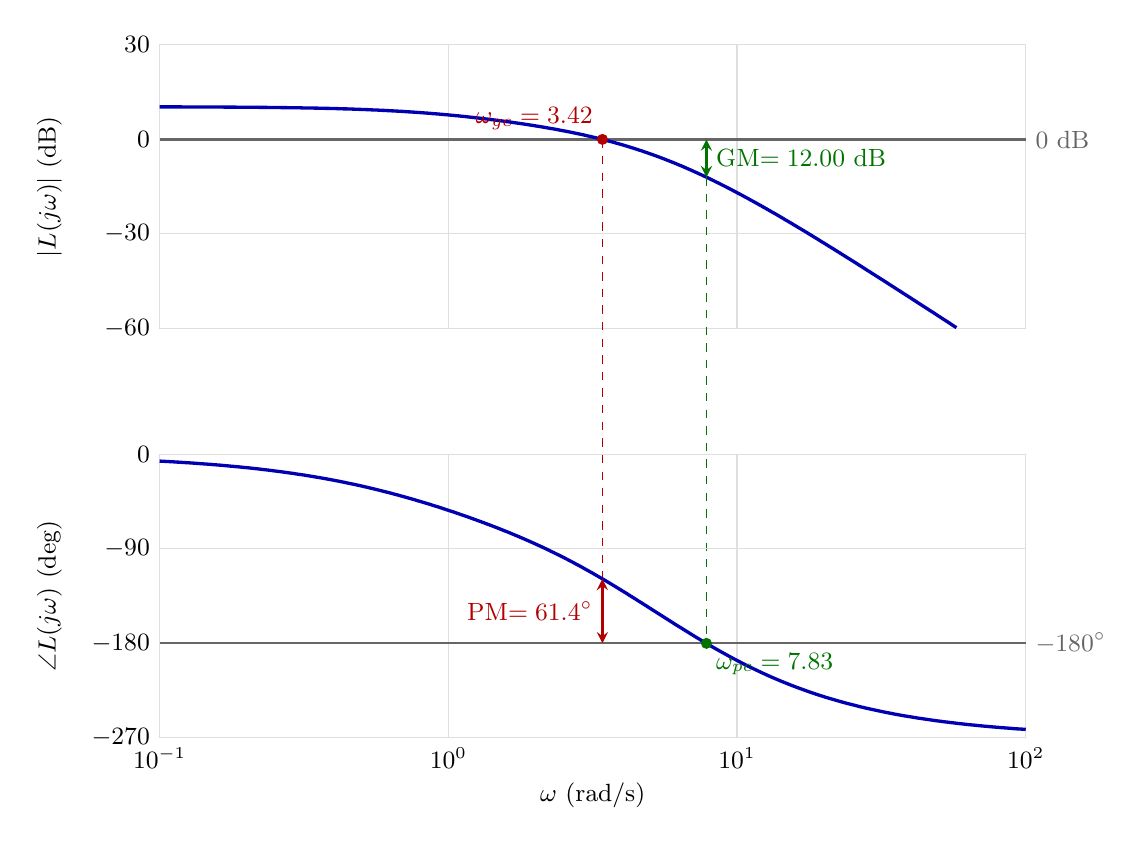
\begin{tikzpicture}[x=1cm,y=1cm,font=\small,>=stealth]
\draw[gray!30] (0,0) rectangle (11.0,3.6);
\draw[gray!25] (0,0.000)--(11.0,0.000); \node[left] at (0,0.000) {$-60$};
\draw[gray!25] (0,1.200)--(11.0,1.200); \node[left] at (0,1.200) {$-30$};
\draw[gray!25] (0,2.400)--(11.0,2.400); \node[left] at (0,2.400) {$0$};
\draw[gray!25] (0,3.600)--(11.0,3.600); \node[left] at (0,3.600) {$30$};
\draw[gray!25] (0.000,0)--(0.000,3.6);
\draw[gray!25] (3.667,0)--(3.667,3.6);
\draw[gray!25] (7.333,0)--(7.333,3.6);
\draw[gray!25] (11.000,0)--(11.000,3.6);
\draw[black!60,thick] (0,2.400)--(11.0,2.400); \node[right,black!60] at (11.0,2.400) {0 dB};
\draw[blue!70!black,very thick] (0.000,2.813) -- (0.027,2.813) -- (0.055,2.813) -- (0.082,2.813) -- (0.110,2.813) -- (0.137,2.813) -- (0.165,2.813) -- (0.192,2.813) -- (0.220,2.813) -- (0.247,2.813) -- (0.275,2.813) -- (0.303,2.812) -- (0.330,2.812) -- (0.358,2.812) -- (0.385,2.812) -- (0.413,2.812) -- (0.440,2.812) -- (0.467,2.812) -- (0.495,2.812) -- (0.522,2.812) -- (0.550,2.812) -- (0.577,2.812) -- (0.605,2.811) -- (0.632,2.811) -- (0.660,2.811) -- (0.688,2.811) -- (0.715,2.811) -- (0.743,2.811) -- (0.770,2.811) -- (0.798,2.811) -- (0.825,2.810) -- (0.853,2.810) -- (0.880,2.810) -- (0.908,2.810) -- (0.935,2.810) -- (0.962,2.810) -- (0.990,2.809) -- (1.018,2.809) -- (1.045,2.809) -- (1.072,2.809) -- (1.100,2.809) -- (1.127,2.808) -- (1.155,2.808) -- (1.182,2.808) -- (1.210,2.808) -- (1.238,2.808) -- (1.265,2.807) -- (1.292,2.807) -- (1.320,2.807) -- (1.347,2.807) -- (1.375,2.806) -- (1.403,2.806) -- (1.430,2.806) -- (1.457,2.805) -- (1.485,2.805) -- (1.512,2.805) -- (1.540,2.804) -- (1.567,2.804) -- (1.595,2.804) -- (1.623,2.803) -- (1.650,2.803) -- (1.677,2.803) -- (1.705,2.802) -- (1.732,2.802) -- (1.760,2.801) -- (1.788,2.801) -- (1.815,2.800) -- (1.842,2.800) -- (1.870,2.799) -- (1.897,2.799) -- (1.925,2.798) -- (1.952,2.798) -- (1.980,2.797) -- (2.007,2.797) -- (2.035,2.796) -- (2.062,2.796) -- (2.090,2.795) -- (2.118,2.794) -- (2.145,2.794) -- (2.172,2.793) -- (2.200,2.792) -- (2.228,2.792) -- (2.255,2.791) -- (2.283,2.790) -- (2.310,2.789) -- (2.337,2.788) -- (2.365,2.788) -- (2.392,2.787) -- (2.420,2.786) -- (2.447,2.785) -- (2.475,2.784) -- (2.502,2.783) -- (2.530,2.782) -- (2.558,2.781) -- (2.585,2.780) -- (2.612,2.779) -- (2.640,2.778) -- (2.667,2.777) -- (2.695,2.775) -- (2.723,2.774) -- (2.750,2.773) -- (2.777,2.772) -- (2.805,2.770) -- (2.832,2.769) -- (2.860,2.768) -- (2.887,2.766) -- (2.915,2.765) -- (2.942,2.763) -- (2.970,2.762) -- (2.998,2.760) -- (3.025,2.759) -- (3.052,2.757) -- (3.080,2.756) -- (3.107,2.754) -- (3.135,2.752) -- (3.163,2.750) -- (3.190,2.749) -- (3.217,2.747) -- (3.245,2.745) -- (3.272,2.743) -- (3.300,2.741) -- (3.327,2.739) -- (3.355,2.737) -- (3.382,2.735) -- (3.410,2.733) -- (3.438,2.731) -- (3.465,2.728) -- (3.492,2.726) -- (3.520,2.724) -- (3.547,2.722) -- (3.575,2.719) -- (3.603,2.717) -- (3.630,2.714) -- (3.658,2.712) -- (3.685,2.709) -- (3.712,2.707) -- (3.740,2.704) -- (3.768,2.701) -- (3.795,2.699) -- (3.822,2.696) -- (3.850,2.693) -- (3.878,2.690) -- (3.905,2.687) -- (3.932,2.684) -- (3.960,2.681) -- (3.987,2.678) -- (4.015,2.675) -- (4.042,2.672) -- (4.070,2.669) -- (4.097,2.666) -- (4.125,2.662) -- (4.152,2.659) -- (4.180,2.656) -- (4.207,2.652) -- (4.235,2.649) -- (4.263,2.645) -- (4.290,2.642) -- (4.317,2.638) -- (4.345,2.635) -- (4.372,2.631) -- (4.400,2.627) -- (4.428,2.624) -- (4.455,2.620) -- (4.482,2.616) -- (4.510,2.612) -- (4.537,2.608) -- (4.565,2.604) -- (4.592,2.600) -- (4.620,2.596) -- (4.647,2.592) -- (4.675,2.588) -- (4.702,2.583) -- (4.730,2.579) -- (4.758,2.575) -- (4.785,2.570) -- (4.812,2.566) -- (4.840,2.561) -- (4.867,2.557) -- (4.895,2.552) -- (4.923,2.547) -- (4.950,2.542) -- (4.977,2.538) -- (5.005,2.533) -- (5.032,2.528) -- (5.060,2.523) -- (5.087,2.517) -- (5.115,2.512) -- (5.143,2.507) -- (5.170,2.502) -- (5.197,2.496) -- (5.225,2.491) -- (5.253,2.485) -- (5.280,2.479) -- (5.308,2.473) -- (5.335,2.468) -- (5.362,2.462) -- (5.390,2.456) -- (5.417,2.449) -- (5.445,2.443) -- (5.472,2.437) -- (5.500,2.430) -- (5.527,2.424) -- (5.555,2.417) -- (5.582,2.410) -- (5.610,2.404) -- (5.638,2.397) -- (5.665,2.389) -- (5.692,2.382) -- (5.720,2.375) -- (5.747,2.368) -- (5.775,2.360) -- (5.803,2.352) -- (5.830,2.345) -- (5.857,2.337) -- (5.885,2.329) -- (5.912,2.321) -- (5.940,2.312) -- (5.967,2.304) -- (5.995,2.295) -- (6.022,2.287) -- (6.050,2.278) -- (6.077,2.269) -- (6.105,2.260) -- (6.133,2.251) -- (6.160,2.241) -- (6.188,2.232) -- (6.215,2.222) -- (6.242,2.213) -- (6.270,2.203) -- (6.297,2.193) -- (6.325,2.183) -- (6.352,2.173) -- (6.380,2.162) -- (6.407,2.152) -- (6.435,2.141) -- (6.462,2.130) -- (6.490,2.119) -- (6.518,2.108) -- (6.545,2.097) -- (6.572,2.086) -- (6.600,2.074) -- (6.628,2.063) -- (6.655,2.051) -- (6.683,2.039) -- (6.710,2.027) -- (6.737,2.015) -- (6.765,2.003) -- (6.792,1.990) -- (6.820,1.978) -- (6.847,1.965) -- (6.875,1.953) -- (6.902,1.940) -- (6.930,1.927) -- (6.957,1.914) -- (6.985,1.901) -- (7.013,1.887) -- (7.040,1.874) -- (7.067,1.860) -- (7.095,1.847) -- (7.122,1.833) -- (7.150,1.819) -- (7.178,1.805) -- (7.205,1.791) -- (7.232,1.777) -- (7.260,1.763) -- (7.287,1.748) -- (7.315,1.734) -- (7.342,1.719) -- (7.370,1.705) -- (7.397,1.690) -- (7.425,1.675) -- (7.453,1.660) -- (7.480,1.645) -- (7.507,1.630) -- (7.535,1.615) -- (7.562,1.600) -- (7.590,1.585) -- (7.617,1.569) -- (7.645,1.554) -- (7.672,1.538) -- (7.700,1.523) -- (7.727,1.507) -- (7.755,1.491) -- (7.782,1.475) -- (7.810,1.460) -- (7.838,1.444) -- (7.865,1.428) -- (7.892,1.412) -- (7.920,1.396) -- (7.947,1.379) -- (7.975,1.363) -- (8.002,1.347) -- (8.030,1.331) -- (8.057,1.314) -- (8.085,1.298) -- (8.112,1.281) -- (8.140,1.265) -- (8.168,1.248) -- (8.195,1.232) -- (8.223,1.215) -- (8.250,1.198) -- (8.277,1.182) -- (8.305,1.165) -- (8.332,1.148) -- (8.360,1.131) -- (8.387,1.114) -- (8.415,1.097) -- (8.443,1.080) -- (8.470,1.063) -- (8.497,1.046) -- (8.525,1.029) -- (8.553,1.012) -- (8.580,0.995) -- (8.607,0.978) -- (8.635,0.961) -- (8.662,0.944) -- (8.690,0.926) -- (8.717,0.909) -- (8.745,0.892) -- (8.772,0.875) -- (8.800,0.857) -- (8.828,0.840) -- (8.855,0.823) -- (8.882,0.805) -- (8.910,0.788) -- (8.938,0.770) -- (8.965,0.753) -- (8.992,0.735) -- (9.020,0.718) -- (9.047,0.700) -- (9.075,0.683) -- (9.102,0.665) -- (9.130,0.648) -- (9.158,0.630) -- (9.185,0.613) -- (9.213,0.595) -- (9.240,0.578) -- (9.267,0.560) -- (9.295,0.542) -- (9.322,0.525) -- (9.350,0.507) -- (9.377,0.489) -- (9.405,0.472) -- (9.432,0.454) -- (9.460,0.436) -- (9.487,0.419) -- (9.515,0.401) -- (9.543,0.383) -- (9.570,0.365) -- (9.598,0.348) -- (9.625,0.330) -- (9.652,0.312) -- (9.680,0.294) -- (9.707,0.277) -- (9.735,0.259) -- (9.762,0.241) -- (9.790,0.223) -- (9.818,0.206) -- (9.845,0.188) -- (9.872,0.170) -- (9.900,0.152) -- (9.928,0.134) -- (9.955,0.116) -- (9.982,0.099) -- (10.010,0.081) -- (10.037,0.063) -- (10.065,0.045) -- (10.092,0.027) -- (10.120,0.009);
\node[rotate=90] at (-1.4,1.8) {$|L(j\omega)|$ (dB)};
\draw[red!70!black,dashed] (5.624,2.400)--(5.624,-3.181);
\fill[red!70!black] (5.624,2.400) circle(2pt); \node[above left,red!70!black] at (5.624,2.400) {$\omega_{gc}=3.42$};
\draw[green!45!black,dashed] (6.945,1.920)--(6.945,-4.000);
\draw[green!45!black,<->,thick] (6.945,1.920)--(6.945,2.400); \node[green!45!black,right] at (6.945,2.160) {GM$=12.00$ dB};
\draw[gray!30] (0,-5.2) rectangle (11.0,-1.6);
\draw[gray!25] (0,-5.200)--(11.0,-5.200); \node[left] at (0,-5.200) {$-270$};
\draw[gray!25] (0,-4.000)--(11.0,-4.000); \node[left] at (0,-4.000) {$-180$};
\draw[gray!25] (0,-2.800)--(11.0,-2.800); \node[left] at (0,-2.800) {$-90$};
\draw[gray!25] (0,-1.600)--(11.0,-1.600); \node[left] at (0,-1.600) {$0$};
\draw[gray!25] (0.000,-5.2)--(0.000,-1.6); \node[below] at (0.000,-5.2) {$10^{-1}$};
\draw[gray!25] (3.667,-5.2)--(3.667,-1.6); \node[below] at (3.667,-5.2) {$10^{0}$};
\draw[gray!25] (7.333,-5.2)--(7.333,-1.6); \node[below] at (7.333,-5.2) {$10^{1}$};
\draw[gray!25] (11.000,-5.2)--(11.000,-1.6); \node[below] at (11.000,-5.2) {$10^{2}$};
\draw[black!60,thick] (0,-4.000)--(11.0,-4.000); \node[right,black!60] at (11.0,-4.000) {$-180^\circ$};
\draw[blue!70!black,very thick] (0.000,-1.685) -- (0.027,-1.687) -- (0.055,-1.688) -- (0.082,-1.690) -- (0.110,-1.691) -- (0.137,-1.693) -- (0.165,-1.694) -- (0.192,-1.696) -- (0.220,-1.698) -- (0.247,-1.699) -- (0.275,-1.701) -- (0.303,-1.703) -- (0.330,-1.705) -- (0.358,-1.706) -- (0.385,-1.708) -- (0.413,-1.710) -- (0.440,-1.712) -- (0.467,-1.714) -- (0.495,-1.716) -- (0.522,-1.718) -- (0.550,-1.720) -- (0.577,-1.722) -- (0.605,-1.724) -- (0.632,-1.726) -- (0.660,-1.728) -- (0.688,-1.731) -- (0.715,-1.733) -- (0.743,-1.735) -- (0.770,-1.737) -- (0.798,-1.740) -- (0.825,-1.742) -- (0.853,-1.745) -- (0.880,-1.747) -- (0.908,-1.750) -- (0.935,-1.752) -- (0.962,-1.755) -- (0.990,-1.757) -- (1.018,-1.760) -- (1.045,-1.763) -- (1.072,-1.766) -- (1.100,-1.768) -- (1.127,-1.771) -- (1.155,-1.774) -- (1.182,-1.777) -- (1.210,-1.780) -- (1.238,-1.783) -- (1.265,-1.786) -- (1.292,-1.790) -- (1.320,-1.793) -- (1.347,-1.796) -- (1.375,-1.799) -- (1.403,-1.803) -- (1.430,-1.806) -- (1.457,-1.810) -- (1.485,-1.813) -- (1.512,-1.817) -- (1.540,-1.820) -- (1.567,-1.824) -- (1.595,-1.828) -- (1.623,-1.832) -- (1.650,-1.836) -- (1.677,-1.839) -- (1.705,-1.843) -- (1.732,-1.848) -- (1.760,-1.852) -- (1.788,-1.856) -- (1.815,-1.860) -- (1.842,-1.864) -- (1.870,-1.869) -- (1.897,-1.873) -- (1.925,-1.878) -- (1.952,-1.882) -- (1.980,-1.887) -- (2.007,-1.892) -- (2.035,-1.896) -- (2.062,-1.901) -- (2.090,-1.906) -- (2.118,-1.911) -- (2.145,-1.916) -- (2.172,-1.921) -- (2.200,-1.926) -- (2.228,-1.932) -- (2.255,-1.937) -- (2.283,-1.942) -- (2.310,-1.948) -- (2.337,-1.953) -- (2.365,-1.959) -- (2.392,-1.965) -- (2.420,-1.971) -- (2.447,-1.976) -- (2.475,-1.982) -- (2.502,-1.988) -- (2.530,-1.994) -- (2.558,-2.000) -- (2.585,-2.007) -- (2.612,-2.013) -- (2.640,-2.019) -- (2.667,-2.026) -- (2.695,-2.032) -- (2.723,-2.039) -- (2.750,-2.046) -- (2.777,-2.052) -- (2.805,-2.059) -- (2.832,-2.066) -- (2.860,-2.073) -- (2.887,-2.080) -- (2.915,-2.087) -- (2.942,-2.094) -- (2.970,-2.102) -- (2.998,-2.109) -- (3.025,-2.116) -- (3.052,-2.124) -- (3.080,-2.132) -- (3.107,-2.139) -- (3.135,-2.147) -- (3.163,-2.155) -- (3.190,-2.163) -- (3.217,-2.170) -- (3.245,-2.178) -- (3.272,-2.187) -- (3.300,-2.195) -- (3.327,-2.203) -- (3.355,-2.211) -- (3.382,-2.220) -- (3.410,-2.228) -- (3.438,-2.236) -- (3.465,-2.245) -- (3.492,-2.254) -- (3.520,-2.262) -- (3.547,-2.271) -- (3.575,-2.280) -- (3.603,-2.289) -- (3.630,-2.298) -- (3.658,-2.307) -- (3.685,-2.316) -- (3.712,-2.325) -- (3.740,-2.334) -- (3.768,-2.344) -- (3.795,-2.353) -- (3.822,-2.363) -- (3.850,-2.372) -- (3.878,-2.382) -- (3.905,-2.391) -- (3.932,-2.401) -- (3.960,-2.411) -- (3.987,-2.421) -- (4.015,-2.431) -- (4.042,-2.441) -- (4.070,-2.451) -- (4.097,-2.461) -- (4.125,-2.471) -- (4.152,-2.482) -- (4.180,-2.492) -- (4.207,-2.502) -- (4.235,-2.513) -- (4.263,-2.524) -- (4.290,-2.534) -- (4.317,-2.545) -- (4.345,-2.556) -- (4.372,-2.567) -- (4.400,-2.578) -- (4.428,-2.589) -- (4.455,-2.600) -- (4.482,-2.612) -- (4.510,-2.623) -- (4.537,-2.635) -- (4.565,-2.646) -- (4.592,-2.658) -- (4.620,-2.670) -- (4.647,-2.682) -- (4.675,-2.694) -- (4.702,-2.706) -- (4.730,-2.718) -- (4.758,-2.731) -- (4.785,-2.743) -- (4.812,-2.756) -- (4.840,-2.768) -- (4.867,-2.781) -- (4.895,-2.794) -- (4.923,-2.807) -- (4.950,-2.820) -- (4.977,-2.834) -- (5.005,-2.847) -- (5.032,-2.861) -- (5.060,-2.874) -- (5.087,-2.888) -- (5.115,-2.902) -- (5.143,-2.916) -- (5.170,-2.930) -- (5.197,-2.944) -- (5.225,-2.959) -- (5.253,-2.973) -- (5.280,-2.988) -- (5.308,-3.003) -- (5.335,-3.017) -- (5.362,-3.032) -- (5.390,-3.048) -- (5.417,-3.063) -- (5.445,-3.078) -- (5.472,-3.094) -- (5.500,-3.109) -- (5.527,-3.125) -- (5.555,-3.141) -- (5.582,-3.157) -- (5.610,-3.173) -- (5.638,-3.189) -- (5.665,-3.205) -- (5.692,-3.221) -- (5.720,-3.238) -- (5.747,-3.254) -- (5.775,-3.271) -- (5.803,-3.288) -- (5.830,-3.305) -- (5.857,-3.321) -- (5.885,-3.338) -- (5.912,-3.355) -- (5.940,-3.372) -- (5.967,-3.390) -- (5.995,-3.407) -- (6.022,-3.424) -- (6.050,-3.441) -- (6.077,-3.459) -- (6.105,-3.476) -- (6.133,-3.493) -- (6.160,-3.511) -- (6.188,-3.528) -- (6.215,-3.546) -- (6.242,-3.563) -- (6.270,-3.581) -- (6.297,-3.598) -- (6.325,-3.616) -- (6.352,-3.633) -- (6.380,-3.651) -- (6.407,-3.668) -- (6.435,-3.686) -- (6.462,-3.703) -- (6.490,-3.721) -- (6.518,-3.738) -- (6.545,-3.756) -- (6.572,-3.773) -- (6.600,-3.790) -- (6.628,-3.807) -- (6.655,-3.824) -- (6.683,-3.841) -- (6.710,-3.858) -- (6.737,-3.875) -- (6.765,-3.892) -- (6.792,-3.909) -- (6.820,-3.926) -- (6.847,-3.942) -- (6.875,-3.959) -- (6.902,-3.975) -- (6.930,-3.991) -- (6.957,-4.008) -- (6.985,-4.024) -- (7.013,-4.040) -- (7.040,-4.056) -- (7.067,-4.071) -- (7.095,-4.087) -- (7.122,-4.102) -- (7.150,-4.118) -- (7.178,-4.133) -- (7.205,-4.148) -- (7.232,-4.163) -- (7.260,-4.178) -- (7.287,-4.193) -- (7.315,-4.207) -- (7.342,-4.222) -- (7.370,-4.236) -- (7.397,-4.250) -- (7.425,-4.264) -- (7.453,-4.278) -- (7.480,-4.292) -- (7.507,-4.305) -- (7.535,-4.319) -- (7.562,-4.332) -- (7.590,-4.345) -- (7.617,-4.358) -- (7.645,-4.371) -- (7.672,-4.384) -- (7.700,-4.396) -- (7.727,-4.409) -- (7.755,-4.421) -- (7.782,-4.433) -- (7.810,-4.445) -- (7.838,-4.457) -- (7.865,-4.468) -- (7.892,-4.480) -- (7.920,-4.491) -- (7.947,-4.502) -- (7.975,-4.513) -- (8.002,-4.524) -- (8.030,-4.535) -- (8.057,-4.545) -- (8.085,-4.556) -- (8.112,-4.566) -- (8.140,-4.576) -- (8.168,-4.586) -- (8.195,-4.596) -- (8.223,-4.606) -- (8.250,-4.616) -- (8.277,-4.625) -- (8.305,-4.634) -- (8.332,-4.644) -- (8.360,-4.653) -- (8.387,-4.662) -- (8.415,-4.670) -- (8.443,-4.679) -- (8.470,-4.688) -- (8.497,-4.696) -- (8.525,-4.704) -- (8.553,-4.712) -- (8.580,-4.720) -- (8.607,-4.728) -- (8.635,-4.736) -- (8.662,-4.744) -- (8.690,-4.751) -- (8.717,-4.759) -- (8.745,-4.766) -- (8.772,-4.773) -- (8.800,-4.780) -- (8.828,-4.787) -- (8.855,-4.794) -- (8.882,-4.801) -- (8.910,-4.808) -- (8.938,-4.814) -- (8.965,-4.821) -- (8.992,-4.827) -- (9.020,-4.833) -- (9.047,-4.839) -- (9.075,-4.845) -- (9.102,-4.851) -- (9.130,-4.857) -- (9.158,-4.863) -- (9.185,-4.869) -- (9.213,-4.874) -- (9.240,-4.880) -- (9.267,-4.885) -- (9.295,-4.890) -- (9.322,-4.896) -- (9.350,-4.901) -- (9.377,-4.906) -- (9.405,-4.911) -- (9.432,-4.916) -- (9.460,-4.921) -- (9.487,-4.925) -- (9.515,-4.930) -- (9.543,-4.934) -- (9.570,-4.939) -- (9.598,-4.943) -- (9.625,-4.948) -- (9.652,-4.952) -- (9.680,-4.956) -- (9.707,-4.960) -- (9.735,-4.964) -- (9.762,-4.968) -- (9.790,-4.972) -- (9.818,-4.976) -- (9.845,-4.980) -- (9.872,-4.984) -- (9.900,-4.987) -- (9.928,-4.991) -- (9.955,-4.995) -- (9.982,-4.998) -- (10.010,-5.001) -- (10.037,-5.005) -- (10.065,-5.008) -- (10.092,-5.011) -- (10.120,-5.015) -- (10.147,-5.018) -- (10.175,-5.021) -- (10.203,-5.024) -- (10.230,-5.027) -- (10.257,-5.030) -- (10.285,-5.033) -- (10.312,-5.036) -- (10.340,-5.038) -- (10.367,-5.041) -- (10.395,-5.044) -- (10.422,-5.047) -- (10.450,-5.049) -- (10.477,-5.052) -- (10.505,-5.054) -- (10.533,-5.057) -- (10.560,-5.059) -- (10.588,-5.062) -- (10.615,-5.064) -- (10.642,-5.066) -- (10.670,-5.069) -- (10.697,-5.071) -- (10.725,-5.073) -- (10.752,-5.075) -- (10.780,-5.077) -- (10.807,-5.079) -- (10.835,-5.082) -- (10.862,-5.084) -- (10.890,-5.086) -- (10.918,-5.087) -- (10.945,-5.089) -- (10.973,-5.091) -- (11.000,-5.093);
\node[rotate=90] at (-1.4,-3.4000000000000004) {$\angle L(j\omega)$ (deg)};
\node[below=0.45cm] at (5.5,-5.2) {$\omega$ (rad/s)};
\draw[red!70!black,<->,thick] (5.624,-3.181)--(5.624,-4.000); \node[red!70!black,left] at (5.624,-3.590) {PM$=61.4^\circ$};
\fill[green!45!black] (6.945,-4.000) circle(2pt); \node[below right,green!45!black] at (6.945,-4.000) {$\omega_{pc}=7.83$};
\end{tikzpicture}
\caption{Bode ของตัวอย่าง 3 ที่ $K=1.979$: GM $=12$ dB ที่ $\omega_{pc}=7.83$ และ PM $\approx61^\circ$ ที่ $\omega_{gc}=3.42$}
\end{figure}

\paragraph{สรุปผล}
$K=1.98$ (สูงสุดที่อนุญาต) $\Rightarrow$ GM $=12$ dB และ PM $\approx61^\circ$ ตรวจด้วย Routh ได้ $K_{\text{crit}}\approx7.88$ จึง GM $=20\log_{10}(7.88/1.979)=12.0$ dB

%=====================================================================
\section{ข้อกำหนดทางความถี่: วงเปิด (OL) วงปิด (CL) กราฟ Polar และ Nichols}

GM และ PM เป็นข้อกำหนดของ \emph{วงเปิด} เท่านั้น ในการออกแบบมักต้องดูข้อกำหนดของ \emph{วงปิด} ควบคู่กันด้วย หัวข้อนี้สรุปนิยาม วิธีคำนวณ และวิธีอ่านค่าจากกราฟ Polar และ Nichols โดยใช้ระบบจากตัวอย่าง 1--3 (ตัวอย่าง 2 และ 3 ใช้ $K$ ที่ออกแบบแล้ว)

\subsection{ข้อกำหนดที่ใช้}
\begin{defbox}{นิยาม}
ให้ $L(\jw)$ เป็น loop gain และ unity feedback จะได้ $T(\jw)=\dfrac{L(\jw)}{1+L(\jw)}$ (ฟังก์ชันถ่ายโอนวงปิด) และ $S(\jw)=\dfrac{1}{1+L(\jw)}$
\begin{description}[leftmargin=1.2em,itemsep=2pt]
\item[วงเปิด (OL)] $\omega_{gc}$, PM, $\omega_{pc}$, GM (ดูหัวข้อ 1) และค่าคงที่ความผิดพลาดตำแหน่ง $K_p=L(0)$ สำหรับระบบประเภท 0 ความผิดพลาดสถานะอยู่ตัวต่อ step หน่วยคือ $e_{ss}=\dfrac{1}{1+K_p}$
\item[วงปิด (CL)] จาก $|T(\jw)|$:
\begin{itemize}[leftmargin=1.2em,itemsep=1pt]
\item $T(0)$: อัตราขยายสถานะอยู่ตัว ($=1-e_{ss}$)
\item $M_r=\max_{\omega}|T(\jw)|$ \emph{resonant peak} และ $\omega_r$ คือความถี่ที่เกิดค่าสูงสุด
\item $\omega_b$ \emph{bandwidth}: ความถี่ที่ $|T|$ ตกลงเหลือ $|T(0)|/\sqrt2$ (ลดลง $3$ dB จากค่าที่ความถี่ต่ำ) ใช้เป็นตัวชี้ความเร็วของผลตอบสนอง
\item $M_s=\max_{\omega}|S(\jw)|$: ยิ่งต่ำ ระยะห่างต่ำสุดจากจุด $-1$ ยิ่งมาก ($d_{\min}=1/M_s$)
\end{itemize}
\end{description}
\end{defbox}

เนื่องจากตัวอย่างทั้งหมดเป็นระบบประเภท 0 ที่ใช้ตัวควบคุมสัดส่วน $T(0)<1$ เสมอ (มี $e_{ss}$) จึงนิยาม $\omega_b$ เทียบกับ $T(0)$ ไม่ใช่เทียบกับ $1$ ($0$ dB)

\subsection{ตัวอย่างการคำนวณ CL ทีละขั้น (ตัวอย่าง 2, $K=0.5614$)}
\paragraph{ขั้น 1: ฟังก์ชันถ่ายโอนวงปิด}
\[
T(s)=\frac{100K}{(s+2)(s+3)(s+4)+100K}=\frac{56.14}{s^{3}+9s^{2}+26s+80.14}
\]

\paragraph{ขั้น 2: ค่าที่ความถี่ต่ำ}
\[
\begin{gathered}
T(0)=\frac{56.14}{80.14}=0.7005\ (-3.09\dB)\\[2pt]
K_p=L(0)=\frac{56.14}{24}=2.339,\qquad e_{ss}=\frac{1}{1+2.339}=0.299
\end{gathered}
\]
นั่นคือผลตอบสนอง step หยุดที่ประมาณ $70\%$ ของค่าที่ต้องการ (ตรงกับ $1-e_{ss}$) เพราะไม่มี integrator

\paragraph{ขั้น 3: Resonant peak}
แทน $s=\jw$ ที่ตัวส่วนของ $T$: $D(\jw)=(80.14-9\omega^2)+j(26\omega-\omega^3)$ จึงได้
\[
|T(\jw)|=\frac{56.14}{\sqrt{Q(\omega)}},\qquad Q(\omega)=(80.14-9\omega^2)^2+(26\omega-\omega^3)^2 .
\]
$|T|$ สูงสุดเมื่อ $Q$ ต่ำสุด สแกนหา (หรือใช้ solver) ได้ $\omega_r\approx3.00$ rad/s ตรวจ:
\[
Q(3)=(80.14-81)^2+(78-27)^2=0.74+2601=2601.7
\ \Rightarrow\ M_r=\frac{56.14}{\sqrt{2601.7}}=1.10\ (0.83\dB)
\]
เมื่อเทียบกับค่า DC: $M_r/T(0)=1.57$ ($3.9$ dB) แสดงว่ามี peaking ชัดเจนแม้ PM จะเท่ากับ $60^\circ$ เพราะ $T(0)$ ต่ำ

\paragraph{ขั้น 4: Bandwidth}
ตั้ง $|T|=T(0)/\sqrt2$ หรือ $Q(\omega)=2\cdot80.14^2=12846$ แก้ได้ $\omega_b\approx4.61$ rad/s ตรวจ: $Q(4.61)=(80.14-191.3)^2+(119.9-98.0)^2=12359+480\approx12840$ ซึ่งใกล้เคียงกับ $12846$ (ผลต่างมาจากการปัดทศนิยม)

\paragraph{ขั้น 5: Sensitivity}
สแกน $|1/(1+L(\jw))|$ ได้ $M_s\approx1.75$ ดังนั้นระยะห่างต่ำสุดจากจุด $-1$ เท่ากับ $1/M_s=0.57$

\subsection{ผลของทั้งสามตัวอย่าง}
\begin{center}
\small
\renewcommand{\arraystretch}{1.25}
\begin{tabular}{@{}lccccccc@{}}
\toprule
 & $K_p$ & $e_{ss}$ & $T(0)$ & $M_r$ & $\omega_r$ & $\omega_b$ & $M_s$ \\
\midrule
ตัวอย่าง 1 & 7.81 & 0.113 & 0.887 & 5.36 (14.6 dB) & 6.54 & 9.58 & 5.87 \\
ตัวอย่าง 2 & 2.34 & 0.299 & 0.701 & 1.10 (0.83 dB) & 3.00 & 4.61 & 1.75 \\
ตัวอย่าง 3 & 3.30 & 0.233 & 0.767 & 1.06 (0.47 dB) & 4.32 & 6.63 & 1.69 \\
\bottomrule
\end{tabular}
\end{center}
ตัวอย่าง 1 มี PM เพียง $12^\circ$ จึงเกิดยอดสูงมากที่วงปิด ($M_r=5.36$, $M_s=5.87$) ผลตอบสนองจะแกว่งแรง ส่วนตัวอย่าง 2 และ 3 ที่ออกแบบให้ PM $\approx60^\circ$ มี $M_r\approx1.1$ และ $M_s\approx1.7$ ซึ่งเป็นช่วงที่ยอมรับได้ทั่วไป $K_p$ ต่ำของตัวอย่าง 2--3 แลกกับ $e_{ss}$ ที่สูงขึ้น (ถ้าต้องการลด $e_{ss}$ ต้องเพิ่ม integrator หรือเพิ่ม $K$ ซึ่งลด margin)

\subsection{กราฟ Polar (Nyquist)}
กราฟ Polar วาด $L(\jw)$ บนระนาบเชิงซ้อน (แกนนอน $\mathrm{Re}\,L$ แกนตั้ง $\mathrm{Im}\,L$) เมื่อ $\omega$ เพิ่มจาก $0$ ถึง $\infty$ อ่านค่าได้ดังนี้
\begin{itemize}[leftmargin=1.2em,itemsep=2pt]
\item $\omega=0$: จุดเริ่มต้นอยู่บนแกนจริงบวกที่ $K_p$ และ $\omega\to\infty$: เส้นโค้งเข้าสู่จุดกำเนิด
\item $\omega_{gc}$: จุดที่เส้นโค้งตัดวงกลมหน่วย $|L|=1$ \; PM คือมุมจากแกนจริงลบไปถึงจุดนั้น
\item $\omega_{pc}$: จุดที่เส้นโค้งตัดแกนจริงลบที่ $-|L(j\omega_{pc})|$ \; $\mathrm{GM}=\dfrac{1}{|L(j\omega_{pc})|}$ (เท่า)
\item ระยะที่ใกล้จุด $-1$ ที่สุดคือ $1/M_s$
\item ผลตอบสนองวงปิด: ค่า $|T|=M$ คงที่ตรงกับ \emph{M-circle} ศูนย์กลาง $\Big(\tfrac{M^2}{1-M^2},0\Big)$ รัศมี $\tfrac{M}{|1-M^2|}$ \; $M_r$ คือ M-circle ที่เส้นโค้งสัมผัสพอดี
\end{itemize}

\begin{figure}[h]
\centering
\begin{tikzpicture}[font=\small,>=stealth]
\clip (-0.8,-0.5) rectangle (12.100000000000001,11.06);
\draw[gray!25] (0,0) rectangle (11.700000000000001,10.66);
\draw[gray!20] (1.300,0)--(1.300,10.66); \node[below] at (1.300,0) {$-1$};
\draw[gray!20] (3.900,0)--(3.900,10.66); \node[below] at (3.900,0) {$0$};
\draw[gray!20] (6.500,0)--(6.500,10.66); \node[below] at (6.500,0) {$1$};
\draw[gray!20] (9.100,0)--(9.100,10.66); \node[below] at (9.100,0) {$2$};
\draw[gray!20] (11.700,0)--(11.700,10.66); \node[below] at (11.700,0) {$3$};
\draw[gray!20] (0,0.520)--(11.700000000000001,0.520); \node[left] at (0,0.520) {$-2$};
\draw[gray!20] (0,3.120)--(11.700000000000001,3.120); \node[left] at (0,3.120) {$-1$};
\draw[gray!20] (0,5.720)--(11.700000000000001,5.720); \node[left] at (0,5.720) {$0$};
\draw[gray!20] (0,8.320)--(11.700000000000001,8.320); \node[left] at (0,8.320) {$1$};
\draw[black!60,thick] (0,5.720)--(11.700000000000001,5.720); \draw[black!60,thick] (3.900,0)--(3.900,10.66);
\draw[black!70,dashed] (6.500,5.720) -- (6.496,5.856) -- (6.486,5.992) -- (6.468,6.127) -- (6.443,6.261) -- (6.411,6.393) -- (6.373,6.523) -- (6.327,6.652) -- (6.275,6.778) -- (6.217,6.900) -- (6.152,7.020) -- (6.081,7.136) -- (6.003,7.248) -- (5.921,7.356) -- (5.832,7.460) -- (5.738,7.558) -- (5.640,7.652) -- (5.536,7.741) -- (5.428,7.823) -- (5.316,7.901) -- (5.200,7.972) -- (5.080,8.037) -- (4.958,8.095) -- (4.832,8.147) -- (4.703,8.193) -- (4.573,8.231) -- (4.441,8.263) -- (4.307,8.288) -- (4.172,8.306) -- (4.036,8.316) -- (3.900,8.320) -- (3.764,8.316) -- (3.628,8.306) -- (3.493,8.288) -- (3.359,8.263) -- (3.227,8.231) -- (3.097,8.193) -- (2.968,8.147) -- (2.842,8.095) -- (2.720,8.037) -- (2.600,7.972) -- (2.484,7.901) -- (2.372,7.823) -- (2.264,7.741) -- (2.160,7.652) -- (2.062,7.558) -- (1.968,7.460) -- (1.879,7.356) -- (1.797,7.248) -- (1.719,7.136) -- (1.648,7.020) -- (1.583,6.900) -- (1.525,6.778) -- (1.473,6.652) -- (1.427,6.523) -- (1.389,6.393) -- (1.357,6.261) -- (1.332,6.127) -- (1.314,5.992) -- (1.304,5.856) -- (1.300,5.720) -- (1.304,5.584) -- (1.314,5.448) -- (1.332,5.313) -- (1.357,5.179) -- (1.389,5.047) -- (1.427,4.917) -- (1.473,4.788) -- (1.525,4.662) -- (1.583,4.540) -- (1.648,4.420) -- (1.719,4.304) -- (1.797,4.192) -- (1.879,4.084) -- (1.968,3.980) -- (2.062,3.882) -- (2.160,3.788) -- (2.264,3.699) -- (2.372,3.617) -- (2.484,3.539) -- (2.600,3.468) -- (2.720,3.403) -- (2.842,3.345) -- (2.968,3.293) -- (3.097,3.247) -- (3.227,3.209) -- (3.359,3.177) -- (3.493,3.152) -- (3.628,3.134) -- (3.764,3.124) -- (3.900,3.120) -- (4.036,3.124) -- (4.172,3.134) -- (4.307,3.152) -- (4.441,3.177) -- (4.573,3.209) -- (4.703,3.247) -- (4.832,3.293) -- (4.958,3.345) -- (5.080,3.403) -- (5.200,3.468) -- (5.316,3.539) -- (5.428,3.617) -- (5.536,3.699) -- (5.640,3.788) -- (5.738,3.882) -- (5.832,3.980) -- (5.921,4.084) -- (6.003,4.192) -- (6.081,4.304) -- (6.152,4.420) -- (6.217,4.540) -- (6.275,4.662) -- (6.327,4.788) -- (6.373,4.917) -- (6.411,5.047) -- (6.443,5.179) -- (6.468,5.313) -- (6.486,5.448) -- (6.496,5.584) -- (6.500,5.720);
\fill[black] (1.300,5.720) circle(2.2pt); \node[above left] at (1.300,5.720) {$-1$};
\node[above left] at (11.700,5.720) {$\mathrm{Re}\,L$}; \node[above] at (4.800,10.660) {$\mathrm{Im}\,L$};
\draw[red!70!black,very thick] (0.006,2.740) -- (0.014,2.768) -- (0.021,2.797) -- (0.028,2.825) -- (0.035,2.853) -- (0.043,2.880) -- (0.050,2.908) -- (0.058,2.936) -- (0.066,2.963) -- (0.074,2.990) -- (0.082,3.017) -- (0.090,3.044) -- (0.098,3.071) -- (0.106,3.098) -- (0.115,3.124) -- (0.123,3.151) -- (0.132,3.177) -- (0.141,3.203) -- (0.149,3.229) -- (0.158,3.255) -- (0.167,3.281) -- (0.176,3.306) -- (0.185,3.332) -- (0.195,3.357) -- (0.204,3.382) -- (0.213,3.407) -- (0.223,3.432) -- (0.232,3.457) -- (0.242,3.482) -- (0.252,3.506) -- (0.261,3.531) -- (0.271,3.555) -- (0.281,3.579) -- (0.291,3.603) -- (0.301,3.627) -- (0.311,3.650) -- (0.322,3.674) -- (0.332,3.697) -- (0.342,3.720) -- (0.353,3.743) -- (0.363,3.766) -- (0.374,3.789) -- (0.385,3.812) -- (0.395,3.834) -- (0.406,3.857) -- (0.417,3.879) -- (0.428,3.901) -- (0.439,3.923) -- (0.450,3.945) -- (0.461,3.967) -- (0.472,3.988) -- (0.483,4.010) -- (0.495,4.031) -- (0.506,4.052) -- (0.517,4.073) -- (0.529,4.094) -- (0.540,4.114) -- (0.552,4.135) -- (0.563,4.155) -- (0.575,4.176) -- (0.586,4.196) -- (0.598,4.216) -- (0.610,4.236) -- (0.622,4.256) -- (0.633,4.275) -- (0.645,4.295) -- (0.657,4.314) -- (0.669,4.333) -- (0.681,4.352) -- (0.693,4.371) -- (0.705,4.390) -- (0.717,4.408) -- (0.730,4.427) -- (0.742,4.445) -- (0.754,4.463) -- (0.766,4.482) -- (0.778,4.500) -- (0.791,4.517) -- (0.803,4.535) -- (0.815,4.553) -- (0.828,4.570) -- (0.840,4.587) -- (0.853,4.604) -- (0.865,4.621) -- (0.877,4.638) -- (0.890,4.655) -- (0.903,4.672) -- (0.915,4.688) -- (0.928,4.705) -- (0.940,4.721) -- (0.953,4.737) -- (0.965,4.753) -- (0.978,4.769) -- (0.991,4.784) -- (1.003,4.800) -- (1.016,4.815) -- (1.029,4.831) -- (1.041,4.846) -- (1.054,4.861) -- (1.067,4.876) -- (1.080,4.891) -- (1.092,4.905) -- (1.105,4.920) -- (1.118,4.934) -- (1.131,4.948) -- (1.143,4.963) -- (1.156,4.977) -- (1.169,4.991) -- (1.182,5.004) -- (1.194,5.018) -- (1.207,5.032) -- (1.220,5.045) -- (1.233,5.058) -- (1.246,5.072) -- (1.258,5.085) -- (1.271,5.098) -- (1.284,5.110) -- (1.297,5.123) -- (1.309,5.136) -- (1.322,5.148) -- (1.335,5.161) -- (1.348,5.173) -- (1.361,5.185) -- (1.373,5.197) -- (1.386,5.209) -- (1.399,5.220) -- (1.411,5.232) -- (1.424,5.244) -- (1.437,5.255) -- (1.450,5.266) -- (1.462,5.278) -- (1.475,5.289) -- (1.488,5.300) -- (1.500,5.311) -- (1.513,5.321) -- (1.525,5.332) -- (1.538,5.342) -- (1.551,5.353) -- (1.563,5.363) -- (1.576,5.373) -- (1.588,5.383) -- (1.601,5.393) -- (1.613,5.403) -- (1.626,5.413) -- (1.638,5.423) -- (1.650,5.432) -- (1.663,5.442) -- (1.675,5.451) -- (1.688,5.460) -- (1.700,5.470) -- (1.712,5.479) -- (1.725,5.488) -- (1.737,5.497) -- (1.749,5.505) -- (1.761,5.514) -- (1.773,5.522) -- (1.786,5.531) -- (1.798,5.539) -- (1.810,5.548) -- (1.822,5.556) -- (1.834,5.564) -- (1.846,5.572) -- (1.858,5.580) -- (1.870,5.587) -- (1.882,5.595) -- (1.894,5.603) -- (1.906,5.610) -- (1.918,5.618) -- (1.929,5.625) -- (1.941,5.632) -- (1.953,5.639) -- (1.965,5.646) -- (1.976,5.653) -- (1.988,5.660) -- (2.000,5.667) -- (2.011,5.674) -- (2.023,5.680) -- (2.034,5.687) -- (2.046,5.693) -- (2.057,5.700) -- (2.069,5.706) -- (2.080,5.712) -- (2.091,5.718) -- (2.103,5.724) -- (2.114,5.730) -- (2.125,5.736) -- (2.136,5.742) -- (2.148,5.748) -- (2.159,5.753) -- (2.170,5.759) -- (2.181,5.764) -- (2.192,5.770) -- (2.203,5.775) -- (2.214,5.780) -- (2.225,5.785) -- (2.235,5.791) -- (2.246,5.796) -- (2.257,5.800) -- (2.268,5.805) -- (2.278,5.810) -- (2.289,5.815) -- (2.300,5.820) -- (2.310,5.824) -- (2.321,5.829) -- (2.331,5.833) -- (2.342,5.837) -- (2.352,5.842) -- (2.363,5.846) -- (2.373,5.850) -- (2.383,5.854) -- (2.393,5.858) -- (2.404,5.862) -- (2.414,5.866) -- (2.424,5.870) -- (2.434,5.874) -- (2.444,5.877) -- (2.454,5.881) -- (2.464,5.885) -- (2.474,5.888) -- (2.484,5.892) -- (2.493,5.895) -- (2.503,5.898) -- (2.513,5.902) -- (2.523,5.905) -- (2.532,5.908) -- (2.542,5.911) -- (2.551,5.914) -- (2.561,5.917) -- (2.570,5.920) -- (2.580,5.923) -- (2.589,5.926) -- (2.599,5.929) -- (2.608,5.931) -- (2.617,5.934) -- (2.626,5.937) -- (2.635,5.939) -- (2.644,5.942) -- (2.654,5.944) -- (2.663,5.946) -- (2.672,5.949) -- (2.680,5.951) -- (2.689,5.953) -- (2.698,5.956) -- (2.707,5.958) -- (2.716,5.960) -- (2.724,5.962) -- (2.733,5.964) -- (2.742,5.966) -- (2.750,5.968) -- (2.759,5.970) -- (2.767,5.971) -- (2.776,5.973) -- (2.784,5.975) -- (2.792,5.977) -- (2.801,5.978) -- (2.809,5.980) -- (2.817,5.981) -- (2.825,5.983) -- (2.834,5.984) -- (2.842,5.986) -- (2.850,5.987) -- (2.858,5.989) -- (2.866,5.990) -- (2.873,5.991) -- (2.881,5.992) -- (2.889,5.994) -- (2.897,5.995) -- (2.905,5.996) -- (2.912,5.997) -- (2.920,5.998) -- (2.927,5.999) -- (2.935,6.000) -- (2.943,6.001) -- (2.950,6.002) -- (2.957,6.003) -- (2.965,6.004) -- (2.972,6.004) -- (2.979,6.005) -- (2.987,6.006) -- (2.994,6.007) -- (3.001,6.007) -- (3.008,6.008) -- (3.015,6.009) -- (3.022,6.009) -- (3.029,6.010) -- (3.036,6.010) -- (3.043,6.011) -- (3.050,6.011) -- (3.057,6.012) -- (3.063,6.012) -- (3.070,6.012) -- (3.077,6.013) -- (3.083,6.013) -- (3.090,6.013) -- (3.097,6.014) -- (3.103,6.014) -- (3.110,6.014) -- (3.116,6.014) -- (3.122,6.014) -- (3.129,6.015) -- (3.135,6.015) -- (3.141,6.015) -- (3.148,6.015) -- (3.154,6.015) -- (3.160,6.015) -- (3.166,6.015) -- (3.172,6.015) -- (3.178,6.015) -- (3.184,6.015) -- (3.190,6.015) -- (3.196,6.015) -- (3.202,6.014) -- (3.208,6.014) -- (3.213,6.014) -- (3.219,6.014) -- (3.225,6.014) -- (3.231,6.013) -- (3.236,6.013) -- (3.242,6.013) -- (3.247,6.013) -- (3.253,6.012) -- (3.258,6.012) -- (3.264,6.012) -- (3.269,6.011) -- (3.274,6.011) -- (3.280,6.011) -- (3.285,6.010) -- (3.290,6.010) -- (3.296,6.009) -- (3.301,6.009) -- (3.306,6.008) -- (3.311,6.008) -- (3.316,6.007) -- (3.321,6.007) -- (3.326,6.006) -- (3.331,6.006) -- (3.336,6.005) -- (3.341,6.005) -- (3.346,6.004) -- (3.350,6.003) -- (3.355,6.003) -- (3.360,6.002) -- (3.365,6.002) -- (3.369,6.001) -- (3.374,6.000) -- (3.379,6.000) -- (3.383,5.999) -- (3.388,5.998) -- (3.392,5.998) -- (3.397,5.997) -- (3.401,5.996) -- (3.406,5.995) -- (3.410,5.995) -- (3.414,5.994) -- (3.419,5.993) -- (3.423,5.992) -- (3.427,5.992) -- (3.431,5.991) -- (3.436,5.990) -- (3.440,5.989) -- (3.444,5.988) -- (3.448,5.988) -- (3.452,5.987) -- (3.456,5.986) -- (3.460,5.985) -- (3.464,5.984) -- (3.468,5.983) -- (3.472,5.982) -- (3.476,5.982) -- (3.479,5.981) -- (3.483,5.980) -- (3.487,5.979) -- (3.491,5.978) -- (3.494,5.977) -- (3.498,5.976) -- (3.502,5.975) -- (3.505,5.974) -- (3.509,5.973) -- (3.513,5.973) -- (3.516,5.972) -- (3.520,5.971) -- (3.523,5.970) -- (3.527,5.969) -- (3.530,5.968) -- (3.533,5.967) -- (3.537,5.966) -- (3.540,5.965) -- (3.543,5.964) -- (3.547,5.963) -- (3.550,5.962) -- (3.553,5.961) -- (3.556,5.960) -- (3.560,5.959) -- (3.563,5.958) -- (3.566,5.957) -- (3.569,5.956) -- (3.572,5.955) -- (3.575,5.954) -- (3.578,5.953) -- (3.581,5.952) -- (3.584,5.951) -- (3.587,5.950) -- (3.590,5.949) -- (3.593,5.948) -- (3.596,5.947) -- (3.599,5.946) -- (3.602,5.945) -- (3.604,5.944) -- (3.607,5.943) -- (3.610,5.942) -- (3.613,5.941) -- (3.615,5.940) -- (3.618,5.939) -- (3.621,5.938) -- (3.623,5.937) -- (3.626,5.936) -- (3.629,5.935) -- (3.631,5.934) -- (3.634,5.933) -- (3.636,5.932) -- (3.639,5.931) -- (3.641,5.930) -- (3.644,5.929) -- (3.646,5.928) -- (3.649,5.926) -- (3.651,5.925) -- (3.654,5.924) -- (3.656,5.923) -- (3.658,5.922) -- (3.661,5.921) -- (3.663,5.920) -- (3.665,5.919) -- (3.667,5.918) -- (3.670,5.917) -- (3.672,5.916) -- (3.674,5.915) -- (3.676,5.914) -- (3.679,5.913) -- (3.681,5.912) -- (3.683,5.911) -- (3.685,5.910) -- (3.687,5.909) -- (3.689,5.908) -- (3.691,5.907) -- (3.693,5.906) -- (3.695,5.905) -- (3.697,5.904) -- (3.699,5.903) -- (3.701,5.902) -- (3.703,5.901) -- (3.705,5.900) -- (3.707,5.899) -- (3.709,5.898) -- (3.711,5.897) -- (3.713,5.896) -- (3.714,5.895) -- (3.716,5.894) -- (3.718,5.893) -- (3.720,5.892) -- (3.722,5.891) -- (3.723,5.890) -- (3.725,5.889) -- (3.727,5.888) -- (3.729,5.887) -- (3.730,5.886) -- (3.732,5.885) -- (3.734,5.885) -- (3.735,5.884) -- (3.737,5.883) -- (3.739,5.882) -- (3.740,5.881) -- (3.742,5.880) -- (3.743,5.879) -- (3.745,5.878) -- (3.746,5.877) -- (3.748,5.876) -- (3.750,5.875) -- (3.751,5.874) -- (3.753,5.873) -- (3.754,5.872) -- (3.755,5.871) -- (3.757,5.871) -- (3.758,5.870) -- (3.760,5.869) -- (3.761,5.868) -- (3.763,5.867) -- (3.764,5.866) -- (3.765,5.865) -- (3.767,5.864) -- (3.768,5.863) -- (3.769,5.862) -- (3.771,5.862) -- (3.772,5.861) -- (3.773,5.860) -- (3.775,5.859) -- (3.776,5.858) -- (3.777,5.857) -- (3.778,5.856) -- (3.780,5.856) -- (3.781,5.855) -- (3.782,5.854) -- (3.783,5.853) -- (3.784,5.852) -- (3.786,5.851) -- (3.787,5.850) -- (3.788,5.850) -- (3.789,5.849) -- (3.790,5.848) -- (3.791,5.847) -- (3.792,5.846) -- (3.794,5.846) -- (3.795,5.845) -- (3.796,5.844) -- (3.797,5.843) -- (3.798,5.842) -- (3.799,5.842) -- (3.800,5.841) -- (3.801,5.840) -- (3.802,5.839) -- (3.803,5.838) -- (3.804,5.838) -- (3.805,5.837) -- (3.806,5.836) -- (3.807,5.835) -- (3.808,5.835) -- (3.809,5.834) -- (3.810,5.833) -- (3.811,5.832) -- (3.812,5.832) -- (3.813,5.831) -- (3.813,5.830) -- (3.814,5.829) -- (3.815,5.829) -- (3.816,5.828) -- (3.817,5.827) -- (3.818,5.826) -- (3.819,5.826) -- (3.820,5.825) -- (3.820,5.824) -- (3.821,5.824) -- (3.822,5.823) -- (3.823,5.822) -- (3.824,5.821) -- (3.824,5.821) -- (3.825,5.820) -- (3.826,5.819) -- (3.827,5.819) -- (3.828,5.818) -- (3.828,5.817) -- (3.829,5.817) -- (3.830,5.816) -- (3.831,5.815) -- (3.831,5.815) -- (3.832,5.814) -- (3.833,5.813) -- (3.833,5.813) -- (3.834,5.812) -- (3.835,5.812) -- (3.835,5.811) -- (3.836,5.810) -- (3.837,5.810) -- (3.837,5.809) -- (3.838,5.808) -- (3.839,5.808) -- (3.839,5.807) -- (3.840,5.807) -- (3.841,5.806) -- (3.841,5.805) -- (3.842,5.805) -- (3.843,5.804) -- (3.843,5.804) -- (3.844,5.803) -- (3.844,5.802) -- (3.845,5.802) -- (3.846,5.801) -- (3.846,5.801) -- (3.847,5.800) -- (3.847,5.799) -- (3.848,5.799) -- (3.848,5.798) -- (3.849,5.798) -- (3.849,5.797) -- (3.850,5.797) -- (3.851,5.796) -- (3.851,5.796) -- (3.852,5.795) -- (3.852,5.794) -- (3.853,5.794) -- (3.853,5.793) -- (3.854,5.793) -- (3.854,5.792) -- (3.855,5.792) -- (3.855,5.791) -- (3.856,5.791) -- (3.856,5.790) -- (3.856,5.790) -- (3.857,5.789) -- (3.857,5.789) -- (3.858,5.788) -- (3.858,5.788) -- (3.859,5.787) -- (3.859,5.787) -- (3.860,5.786) -- (3.860,5.786) -- (3.860,5.785) -- (3.861,5.785) -- (3.861,5.784) -- (3.862,5.784) -- (3.862,5.783) -- (3.863,5.783) -- (3.863,5.782) -- (3.863,5.782) -- (3.864,5.782) -- (3.864,5.781) -- (3.865,5.781) -- (3.865,5.780) -- (3.865,5.780) -- (3.866,5.779) -- (3.866,5.779) -- (3.866,5.778) -- (3.867,5.778) -- (3.867,5.778) -- (3.867,5.777) -- (3.868,5.777) -- (3.868,5.776) -- (3.869,5.776) -- (3.869,5.775) -- (3.869,5.775) -- (3.870,5.775) -- (3.870,5.774) -- (3.870,5.774) -- (3.871,5.773) -- (3.871,5.773) -- (3.871,5.773) -- (3.871,5.772) -- (3.872,5.772) -- (3.872,5.771) -- (3.872,5.771) -- (3.873,5.771) -- (3.873,5.770) -- (3.873,5.770) -- (3.874,5.769) -- (3.874,5.769) -- (3.874,5.769) -- (3.874,5.768) -- (3.875,5.768) -- (3.875,5.768) -- (3.875,5.767) -- (3.875,5.767) -- (3.876,5.767) -- (3.876,5.766) -- (3.876,5.766) -- (3.877,5.765) -- (3.877,5.765) -- (3.877,5.765) -- (3.877,5.764) -- (3.878,5.764) -- (3.878,5.764) -- (3.878,5.763) -- (3.878,5.763) -- (3.879,5.763) -- (3.879,5.762) -- (3.879,5.762) -- (3.879,5.762) -- (3.879,5.761) -- (3.880,5.761) -- (3.880,5.761) -- (3.880,5.761) -- (3.880,5.760) -- (3.881,5.760) -- (3.881,5.760) -- (3.881,5.759) -- (3.881,5.759) -- (3.881,5.759) -- (3.882,5.758) -- (3.882,5.758) -- (3.882,5.758) -- (3.882,5.757) -- (3.882,5.757) -- (3.883,5.757) -- (3.883,5.757) -- (3.883,5.756) -- (3.883,5.756) -- (3.883,5.756) -- (3.883,5.755) -- (3.884,5.755) -- (3.884,5.755) -- (3.884,5.755) -- (3.884,5.754) -- (3.884,5.754) -- (3.885,5.754) -- (3.885,5.754) -- (3.885,5.753) -- (3.885,5.753) -- (3.885,5.753) -- (3.885,5.753) -- (3.886,5.752) -- (3.886,5.752) -- (3.886,5.752) -- (3.886,5.752) -- (3.886,5.751) -- (3.886,5.751) -- (3.886,5.751) -- (3.887,5.751) -- (3.887,5.750) -- (3.887,5.750) -- (3.887,5.750) -- (3.887,5.750) -- (3.887,5.749) -- (3.887,5.749) -- (3.888,5.749) -- (3.888,5.749) -- (3.888,5.748) -- (3.888,5.748) -- (3.888,5.748) -- (3.888,5.748) -- (3.888,5.748) -- (3.889,5.747) -- (3.889,5.747) -- (3.889,5.747) -- (3.889,5.747) -- (3.889,5.746) -- (3.889,5.746) -- (3.889,5.746) -- (3.889,5.746) -- (3.890,5.746) -- (3.890,5.745) -- (3.890,5.745) -- (3.890,5.745) -- (3.890,5.745) -- (3.890,5.745) -- (3.890,5.744) -- (3.890,5.744) -- (3.890,5.744) -- (3.891,5.744) -- (3.891,5.744) -- (3.891,5.743) -- (3.891,5.743) -- (3.891,5.743) -- (3.891,5.743) -- (3.891,5.743) -- (3.891,5.743) -- (3.891,5.742) -- (3.891,5.742) -- (3.892,5.742) -- (3.892,5.742) -- (3.892,5.742) -- (3.892,5.741) -- (3.892,5.741) -- (3.892,5.741) -- (3.892,5.741) -- (3.892,5.741) -- (3.892,5.741) -- (3.892,5.740) -- (3.892,5.740) -- (3.893,5.740) -- (3.893,5.740) -- (3.893,5.740) -- (3.893,5.740) -- (3.893,5.739) -- (3.893,5.739) -- (3.893,5.739) -- (3.893,5.739) -- (3.893,5.739) -- (3.893,5.739) -- (3.893,5.739) -- (3.893,5.738) -- (3.893,5.738) -- (3.894,5.738) -- (3.894,5.738) -- (3.894,5.738) -- (3.894,5.738) -- (3.894,5.738) -- (3.894,5.737) -- (3.894,5.737) -- (3.894,5.737) -- (3.894,5.737) -- (3.894,5.737) -- (3.894,5.737) -- (3.894,5.737) -- (3.894,5.736) -- (3.894,5.736) -- (3.894,5.736) -- (3.895,5.736) -- (3.895,5.736) -- (3.895,5.736) -- (3.895,5.736) -- (3.895,5.736) -- (3.895,5.735) -- (3.895,5.735) -- (3.895,5.735) -- (3.895,5.735) -- (3.895,5.735) -- (3.895,5.735) -- (3.895,5.735) -- (3.895,5.735) -- (3.895,5.734) -- (3.895,5.734) -- (3.895,5.734) -- (3.895,5.734) -- (3.895,5.734) -- (3.896,5.734) -- (3.896,5.734) -- (3.896,5.734) -- (3.896,5.733) -- (3.896,5.733) -- (3.896,5.733) -- (3.896,5.733) -- (3.896,5.733) -- (3.896,5.733) -- (3.896,5.733) -- (3.896,5.733) -- (3.896,5.733) -- (3.896,5.733) -- (3.896,5.732) -- (3.896,5.732) -- (3.896,5.732) -- (3.896,5.732) -- (3.896,5.732) -- (3.896,5.732) -- (3.896,5.732) -- (3.896,5.732) -- (3.896,5.732) -- (3.897,5.732) -- (3.897,5.731) -- (3.897,5.731) -- (3.897,5.731) -- (3.897,5.731) -- (3.897,5.731) -- (3.897,5.731) -- (3.897,5.731) -- (3.897,5.731) -- (3.897,5.731) -- (3.897,5.731) -- (3.897,5.731) -- (3.897,5.730) -- (3.897,5.730) -- (3.897,5.730) -- (3.897,5.730) -- (3.897,5.730) -- (3.897,5.730) -- (3.897,5.730) -- (3.897,5.730) -- (3.897,5.730) -- (3.897,5.730) -- (3.897,5.730) -- (3.897,5.730) -- (3.897,5.729) -- (3.897,5.729) -- (3.897,5.729) -- (3.897,5.729) -- (3.897,5.729) -- (3.897,5.729) -- (3.898,5.729) -- (3.898,5.729) -- (3.898,5.729) -- (3.898,5.729) -- (3.898,5.729) -- (3.898,5.729) -- (3.898,5.729) -- (3.898,5.728) -- (3.898,5.728) -- (3.898,5.728) -- (3.898,5.728) -- (3.898,5.728) -- (3.898,5.728) -- (3.898,5.728) -- (3.898,5.728) -- (3.898,5.728) -- (3.898,5.728) -- (3.898,5.728) -- (3.898,5.728) -- (3.898,5.728) -- (3.898,5.728) -- (3.898,5.728) -- (3.898,5.727) -- (3.898,5.727) -- (3.898,5.727) -- (3.898,5.727) -- (3.898,5.727) -- (3.898,5.727) -- (3.898,5.727) -- (3.898,5.727) -- (3.898,5.727) -- (3.898,5.727) -- (3.898,5.727) -- (3.898,5.727) -- (3.898,5.727) -- (3.898,5.727) -- (3.898,5.727) -- (3.898,5.727) -- (3.898,5.727) -- (3.898,5.726) -- (3.898,5.726) -- (3.898,5.726) -- (3.898,5.726) -- (3.898,5.726) -- (3.898,5.726) -- (3.899,5.726) -- (3.899,5.726) -- (3.899,5.726) -- (3.899,5.726) -- (3.899,5.726) -- (3.899,5.726) -- (3.899,5.726) -- (3.899,5.726) -- (3.899,5.726) -- (3.899,5.726) -- (3.899,5.726) -- (3.899,5.726) -- (3.899,5.726) -- (3.899,5.726) -- (3.899,5.725) -- (3.899,5.725) -- (3.899,5.725) -- (3.899,5.725) -- (3.899,5.725) -- (3.899,5.725) -- (3.899,5.725) -- (3.899,5.725) -- (3.899,5.725) -- (3.899,5.725) -- (3.899,5.725) -- (3.899,5.725) -- (3.899,5.725) -- (3.899,5.725) -- (3.899,5.725) -- (3.899,5.725) -- (3.899,5.725) -- (3.899,5.725) -- (3.899,5.725) -- (3.899,5.725) -- (3.899,5.725) -- (3.899,5.725) -- (3.899,5.725) -- (3.899,5.725) -- (3.899,5.724) -- (3.899,5.724) -- (3.899,5.724) -- (3.899,5.724) -- (3.899,5.724) -- (3.899,5.724) -- (3.899,5.724) -- (3.899,5.724) -- (3.899,5.724) -- (3.899,5.724) -- (3.899,5.724) -- (3.899,5.724) -- (3.899,5.724) -- (3.899,5.724) -- (3.899,5.724) -- (3.899,5.724) -- (3.899,5.724) -- (3.899,5.724) -- (3.899,5.724) -- (3.899,5.724) -- (3.899,5.724) -- (3.899,5.724) -- (3.899,5.724) -- (3.899,5.724) -- (3.899,5.724) -- (3.899,5.724) -- (3.899,5.724) -- (3.899,5.724) -- (3.899,5.724) -- (3.899,5.724) -- (3.899,5.723) -- (3.899,5.723) -- (3.899,5.723) -- (3.899,5.723) -- (3.899,5.723) -- (3.899,5.723) -- (3.899,5.723) -- (3.899,5.723) -- (3.899,5.723) -- (3.899,5.723) -- (3.899,5.723) -- (3.899,5.723) -- (3.899,5.723) -- (3.899,5.723) -- (3.899,5.723) -- (3.899,5.723) -- (3.899,5.723) -- (3.899,5.723) -- (3.899,5.723) -- (3.899,5.723) -- (3.899,5.723) -- (3.899,5.723) -- (3.899,5.723) -- (3.899,5.723) -- (3.899,5.723) -- (3.899,5.723) -- (3.899,5.723) -- (3.899,5.723) -- (3.900,5.723) -- (3.900,5.723) -- (3.900,5.723) -- (3.900,5.723) -- (3.900,5.723) -- (3.900,5.723) -- (3.900,5.723) -- (3.900,5.723) -- (3.900,5.723) -- (3.900,5.723) -- (3.900,5.723) -- (3.900,5.722) -- (3.900,5.722) -- (3.900,5.722) -- (3.900,5.722) -- (3.900,5.722) -- (3.900,5.722) -- (3.900,5.722) -- (3.900,5.722) -- (3.900,5.722) -- (3.900,5.722) -- (3.900,5.722) -- (3.900,5.722) -- (3.900,5.722) -- (3.900,5.722) -- (3.900,5.722) -- (3.900,5.722) -- (3.900,5.722) -- (3.900,5.722) -- (3.900,5.722) -- (3.900,5.722) -- (3.900,5.722) -- (3.900,5.722) -- (3.900,5.722) -- (3.900,5.722) -- (3.900,5.722) -- (3.900,5.722) -- (3.900,5.722) -- (3.900,5.722) -- (3.900,5.722) -- (3.900,5.722) -- (3.900,5.722) -- (3.900,5.722) -- (3.900,5.722) -- (3.900,5.722) -- (3.900,5.722) -- (3.900,5.722) -- (3.900,5.722) -- (3.900,5.722) -- (3.900,5.722) -- (3.900,5.722) -- (3.900,5.722) -- (3.900,5.722) -- (3.900,5.722) -- (3.900,5.722) -- (3.900,5.722) -- (3.900,5.722) -- (3.900,5.722) -- (3.900,5.722) -- (3.900,5.722) -- (3.900,5.722) -- (3.900,5.722) -- (3.900,5.722) -- (3.900,5.722) -- (3.900,5.722) -- (3.900,5.722) -- (3.900,5.722) -- (3.900,5.722) -- (3.900,5.722) -- (3.900,5.722) -- (3.900,5.722) -- (3.900,5.721) -- (3.900,5.721) -- (3.900,5.721) -- (3.900,5.721) -- (3.900,5.721) -- (3.900,5.721) -- (3.900,5.721) -- (3.900,5.721) -- (3.900,5.721) -- (3.900,5.721) -- (3.900,5.721) -- (3.900,5.721) -- (3.900,5.721) -- (3.900,5.721) -- (3.900,5.721) -- (3.900,5.721) -- (3.900,5.721) -- (3.900,5.721) -- (3.900,5.721);
\fill[red!70!black] (1.356,5.181) circle(2.6pt);
\draw[red!70!black,fill=white,thick] (2.024,5.650) rectangle (2.164,5.790);
\draw[red!70!black,very thick] (8.300,10.010)--(8.800,10.010); \node[right] at (8.850,10.010) {ตัวอย่าง 1};
\draw[blue!70!black,very thick] (9.982,5.713) -- (9.982,5.713) -- (9.982,5.713) -- (9.982,5.713) -- (9.982,5.713) -- (9.982,5.713) -- (9.982,5.713) -- (9.982,5.713) -- (9.982,5.713) -- (9.982,5.713) -- (9.982,5.713) -- (9.982,5.713) -- (9.982,5.713) -- (9.982,5.713) -- (9.982,5.713) -- (9.982,5.713) -- (9.982,5.713) -- (9.982,5.713) -- (9.982,5.713) -- (9.982,5.713) -- (9.982,5.713) -- (9.982,5.713) -- (9.982,5.713) -- (9.982,5.713) -- (9.982,5.713) -- (9.982,5.713) -- (9.982,5.713) -- (9.982,5.713) -- (9.982,5.713) -- (9.982,5.713) -- (9.982,5.713) -- (9.982,5.713) -- (9.982,5.713) -- (9.982,5.713) -- (9.982,5.713) -- (9.982,5.713) -- (9.982,5.713) -- (9.982,5.713) -- (9.982,5.713) -- (9.982,5.713) -- (9.982,5.713) -- (9.982,5.713) -- (9.982,5.713) -- (9.982,5.713) -- (9.982,5.713) -- (9.982,5.712) -- (9.982,5.712) -- (9.982,5.712) -- (9.982,5.712) -- (9.982,5.712) -- (9.982,5.712) -- (9.982,5.712) -- (9.982,5.712) -- (9.982,5.712) -- (9.982,5.712) -- (9.982,5.712) -- (9.982,5.712) -- (9.982,5.712) -- (9.982,5.712) -- (9.982,5.712) -- (9.982,5.712) -- (9.982,5.712) -- (9.982,5.712) -- (9.982,5.712) -- (9.982,5.712) -- (9.982,5.712) -- (9.982,5.712) -- (9.982,5.712) -- (9.982,5.712) -- (9.982,5.712) -- (9.982,5.712) -- (9.982,5.712) -- (9.982,5.712) -- (9.982,5.712) -- (9.982,5.712) -- (9.982,5.712) -- (9.982,5.712) -- (9.982,5.712) -- (9.982,5.712) -- (9.982,5.712) -- (9.982,5.712) -- (9.982,5.712) -- (9.982,5.712) -- (9.982,5.712) -- (9.982,5.712) -- (9.982,5.712) -- (9.982,5.712) -- (9.982,5.712) -- (9.982,5.712) -- (9.982,5.711) -- (9.982,5.711) -- (9.982,5.711) -- (9.982,5.711) -- (9.982,5.711) -- (9.982,5.711) -- (9.982,5.711) -- (9.982,5.711) -- (9.982,5.711) -- (9.982,5.711) -- (9.982,5.711) -- (9.982,5.711) -- (9.982,5.711) -- (9.982,5.711) -- (9.982,5.711) -- (9.982,5.711) -- (9.982,5.711) -- (9.982,5.711) -- (9.982,5.711) -- (9.982,5.711) -- (9.982,5.711) -- (9.982,5.711) -- (9.982,5.711) -- (9.982,5.711) -- (9.982,5.711) -- (9.982,5.711) -- (9.982,5.711) -- (9.982,5.711) -- (9.982,5.711) -- (9.982,5.711) -- (9.982,5.711) -- (9.982,5.711) -- (9.982,5.711) -- (9.982,5.711) -- (9.982,5.711) -- (9.982,5.711) -- (9.982,5.711) -- (9.982,5.711) -- (9.982,5.711) -- (9.982,5.710) -- (9.982,5.710) -- (9.982,5.710) -- (9.982,5.710) -- (9.982,5.710) -- (9.982,5.710) -- (9.982,5.710) -- (9.982,5.710) -- (9.982,5.710) -- (9.982,5.710) -- (9.982,5.710) -- (9.982,5.710) -- (9.982,5.710) -- (9.982,5.710) -- (9.982,5.710) -- (9.982,5.710) -- (9.982,5.710) -- (9.982,5.710) -- (9.982,5.710) -- (9.982,5.710) -- (9.982,5.710) -- (9.982,5.710) -- (9.982,5.710) -- (9.982,5.710) -- (9.982,5.710) -- (9.982,5.710) -- (9.982,5.710) -- (9.982,5.710) -- (9.982,5.710) -- (9.982,5.710) -- (9.982,5.710) -- (9.982,5.710) -- (9.982,5.710) -- (9.982,5.710) -- (9.982,5.709) -- (9.982,5.709) -- (9.982,5.709) -- (9.982,5.709) -- (9.982,5.709) -- (9.982,5.709) -- (9.982,5.709) -- (9.982,5.709) -- (9.982,5.709) -- (9.982,5.709) -- (9.982,5.709) -- (9.982,5.709) -- (9.982,5.709) -- (9.982,5.709) -- (9.982,5.709) -- (9.982,5.709) -- (9.982,5.709) -- (9.982,5.709) -- (9.982,5.709) -- (9.982,5.709) -- (9.982,5.709) -- (9.982,5.709) -- (9.982,5.709) -- (9.982,5.709) -- (9.982,5.709) -- (9.982,5.709) -- (9.982,5.709) -- (9.982,5.709) -- (9.982,5.709) -- (9.982,5.709) -- (9.982,5.709) -- (9.982,5.709) -- (9.982,5.708) -- (9.982,5.708) -- (9.982,5.708) -- (9.982,5.708) -- (9.982,5.708) -- (9.982,5.708) -- (9.982,5.708) -- (9.982,5.708) -- (9.982,5.708) -- (9.982,5.708) -- (9.982,5.708) -- (9.982,5.708) -- (9.982,5.708) -- (9.982,5.708) -- (9.982,5.708) -- (9.982,5.708) -- (9.982,5.708) -- (9.982,5.708) -- (9.982,5.708) -- (9.982,5.708) -- (9.982,5.708) -- (9.982,5.708) -- (9.982,5.708) -- (9.982,5.708) -- (9.982,5.708) -- (9.982,5.708) -- (9.982,5.708) -- (9.982,5.708) -- (9.982,5.708) -- (9.982,5.707) -- (9.982,5.707) -- (9.982,5.707) -- (9.982,5.707) -- (9.982,5.707) -- (9.982,5.707) -- (9.982,5.707) -- (9.982,5.707) -- (9.982,5.707) -- (9.982,5.707) -- (9.982,5.707) -- (9.982,5.707) -- (9.982,5.707) -- (9.982,5.707) -- (9.982,5.707) -- (9.982,5.707) -- (9.982,5.707) -- (9.982,5.707) -- (9.982,5.707) -- (9.982,5.707) -- (9.982,5.707) -- (9.982,5.707) -- (9.982,5.707) -- (9.982,5.707) -- (9.982,5.707) -- (9.982,5.707) -- (9.982,5.707) -- (9.982,5.706) -- (9.982,5.706) -- (9.982,5.706) -- (9.982,5.706) -- (9.982,5.706) -- (9.982,5.706) -- (9.982,5.706) -- (9.982,5.706) -- (9.982,5.706) -- (9.982,5.706) -- (9.982,5.706) -- (9.982,5.706) -- (9.982,5.706) -- (9.982,5.706) -- (9.982,5.706) -- (9.982,5.706) -- (9.982,5.706) -- (9.982,5.706) -- (9.982,5.706) -- (9.982,5.706) -- (9.982,5.706) -- (9.982,5.706) -- (9.982,5.706) -- (9.982,5.706) -- (9.982,5.706) -- (9.982,5.705) -- (9.982,5.705) -- (9.982,5.705) -- (9.982,5.705) -- (9.982,5.705) -- (9.982,5.705) -- (9.982,5.705) -- (9.982,5.705) -- (9.982,5.705) -- (9.982,5.705) -- (9.982,5.705) -- (9.982,5.705) -- (9.982,5.705) -- (9.982,5.705) -- (9.982,5.705) -- (9.982,5.705) -- (9.982,5.705) -- (9.982,5.705) -- (9.982,5.705) -- (9.982,5.705) -- (9.982,5.705) -- (9.982,5.705) -- (9.982,5.705) -- (9.982,5.704) -- (9.982,5.704) -- (9.982,5.704) -- (9.982,5.704) -- (9.982,5.704) -- (9.982,5.704) -- (9.982,5.704) -- (9.982,5.704) -- (9.982,5.704) -- (9.982,5.704) -- (9.982,5.704) -- (9.982,5.704) -- (9.982,5.704) -- (9.982,5.704) -- (9.982,5.704) -- (9.982,5.704) -- (9.982,5.704) -- (9.982,5.704) -- (9.982,5.704) -- (9.982,5.704) -- (9.982,5.704) -- (9.982,5.703) -- (9.982,5.703) -- (9.982,5.703) -- (9.982,5.703) -- (9.982,5.703) -- (9.982,5.703) -- (9.982,5.703) -- (9.982,5.703) -- (9.982,5.703) -- (9.982,5.703) -- (9.982,5.703) -- (9.982,5.703) -- (9.982,5.703) -- (9.982,5.703) -- (9.982,5.703) -- (9.982,5.703) -- (9.982,5.703) -- (9.982,5.703) -- (9.982,5.703) -- (9.982,5.703) -- (9.982,5.703) -- (9.982,5.702) -- (9.982,5.702) -- (9.982,5.702) -- (9.982,5.702) -- (9.982,5.702) -- (9.982,5.702) -- (9.982,5.702) -- (9.982,5.702) -- (9.982,5.702) -- (9.982,5.702) -- (9.982,5.702) -- (9.982,5.702) -- (9.982,5.702) -- (9.982,5.702) -- (9.982,5.702) -- (9.982,5.702) -- (9.982,5.702) -- (9.982,5.702) -- (9.982,5.702) -- (9.982,5.701) -- (9.982,5.701) -- (9.982,5.701) -- (9.982,5.701) -- (9.982,5.701) -- (9.982,5.701) -- (9.982,5.701) -- (9.982,5.701) -- (9.982,5.701) -- (9.982,5.701) -- (9.982,5.701) -- (9.982,5.701) -- (9.982,5.701) -- (9.982,5.701) -- (9.982,5.701) -- (9.982,5.701) -- (9.982,5.701) -- (9.982,5.701) -- (9.982,5.700) -- (9.982,5.700) -- (9.982,5.700) -- (9.982,5.700) -- (9.982,5.700) -- (9.982,5.700) -- (9.982,5.700) -- (9.982,5.700) -- (9.982,5.700) -- (9.982,5.700) -- (9.982,5.700) -- (9.982,5.700) -- (9.982,5.700) -- (9.982,5.700) -- (9.982,5.700) -- (9.982,5.700) -- (9.982,5.700) -- (9.982,5.700) -- (9.982,5.699) -- (9.982,5.699) -- (9.982,5.699) -- (9.982,5.699) -- (9.982,5.699) -- (9.982,5.699) -- (9.982,5.699) -- (9.982,5.699) -- (9.982,5.699) -- (9.982,5.699) -- (9.982,5.699) -- (9.982,5.699) -- (9.982,5.699) -- (9.982,5.699) -- (9.982,5.699) -- (9.982,5.699) -- (9.982,5.698) -- (9.982,5.698) -- (9.982,5.698) -- (9.982,5.698) -- (9.982,5.698) -- (9.982,5.698) -- (9.982,5.698) -- (9.982,5.698) -- (9.982,5.698) -- (9.982,5.698) -- (9.982,5.698) -- (9.982,5.698) -- (9.982,5.698) -- (9.982,5.698) -- (9.982,5.698) -- (9.982,5.698) -- (9.982,5.697) -- (9.982,5.697) -- (9.982,5.697) -- (9.982,5.697) -- (9.982,5.697) -- (9.982,5.697) -- (9.982,5.697) -- (9.982,5.697) -- (9.982,5.697) -- (9.982,5.697) -- (9.982,5.697) -- (9.982,5.697) -- (9.982,5.697) -- (9.982,5.697) -- (9.982,5.697) -- (9.982,5.696) -- (9.982,5.696) -- (9.982,5.696) -- (9.982,5.696) -- (9.982,5.696) -- (9.982,5.696) -- (9.982,5.696) -- (9.982,5.696) -- (9.982,5.696) -- (9.982,5.696) -- (9.982,5.696) -- (9.982,5.696) -- (9.982,5.696) -- (9.982,5.696) -- (9.982,5.696) -- (9.982,5.695) -- (9.982,5.695) -- (9.982,5.695) -- (9.982,5.695) -- (9.982,5.695) -- (9.982,5.695) -- (9.982,5.695) -- (9.982,5.695) -- (9.982,5.695) -- (9.982,5.695) -- (9.982,5.695) -- (9.982,5.695) -- (9.982,5.695) -- (9.982,5.695) -- (9.982,5.694) -- (9.982,5.694) -- (9.982,5.694) -- (9.982,5.694) -- (9.982,5.694) -- (9.982,5.694) -- (9.982,5.694) -- (9.982,5.694) -- (9.982,5.694) -- (9.982,5.694) -- (9.982,5.694) -- (9.982,5.694) -- (9.982,5.694) -- (9.982,5.693) -- (9.982,5.693) -- (9.982,5.693) -- (9.982,5.693) -- (9.982,5.693) -- (9.982,5.693) -- (9.982,5.693) -- (9.982,5.693) -- (9.982,5.693) -- (9.982,5.693) -- (9.982,5.693) -- (9.982,5.693) -- (9.982,5.693) -- (9.982,5.692) -- (9.982,5.692) -- (9.982,5.692) -- (9.982,5.692) -- (9.982,5.692) -- (9.982,5.692) -- (9.982,5.692) -- (9.982,5.692) -- (9.982,5.692) -- (9.982,5.692) -- (9.982,5.692) -- (9.982,5.692) -- (9.982,5.691) -- (9.982,5.691) -- (9.982,5.691) -- (9.982,5.691) -- (9.982,5.691) -- (9.982,5.691) -- (9.982,5.691) -- (9.982,5.691) -- (9.982,5.691) -- (9.982,5.691) -- (9.982,5.691) -- (9.982,5.691) -- (9.982,5.690) -- (9.982,5.690) -- (9.982,5.690) -- (9.982,5.690) -- (9.982,5.690) -- (9.982,5.690) -- (9.982,5.690) -- (9.982,5.690) -- (9.982,5.690) -- (9.982,5.690) -- (9.982,5.690) -- (9.982,5.690) -- (9.982,5.689) -- (9.982,5.689) -- (9.982,5.689) -- (9.982,5.689) -- (9.982,5.689) -- (9.982,5.689) -- (9.982,5.689) -- (9.982,5.689) -- (9.982,5.689) -- (9.982,5.689) -- (9.982,5.689) -- (9.982,5.688) -- (9.982,5.688) -- (9.982,5.688) -- (9.982,5.688) -- (9.982,5.688) -- (9.982,5.688) -- (9.982,5.688) -- (9.982,5.688) -- (9.982,5.688) -- (9.982,5.688) -- (9.982,5.688) -- (9.982,5.687) -- (9.982,5.687) -- (9.982,5.687) -- (9.982,5.687) -- (9.982,5.687) -- (9.982,5.687) -- (9.982,5.687) -- (9.982,5.687) -- (9.982,5.687) -- (9.982,5.687) -- (9.982,5.686) -- (9.982,5.686) -- (9.982,5.686) -- (9.982,5.686) -- (9.982,5.686) -- (9.982,5.686) -- (9.982,5.686) -- (9.982,5.686) -- (9.982,5.686) -- (9.982,5.686) -- (9.982,5.686) -- (9.982,5.685) -- (9.982,5.685) -- (9.982,5.685) -- (9.982,5.685) -- (9.982,5.685) -- (9.982,5.685) -- (9.982,5.685) -- (9.982,5.685) -- (9.982,5.685) -- (9.982,5.685) -- (9.982,5.684) -- (9.982,5.684) -- (9.982,5.684) -- (9.982,5.684) -- (9.982,5.684) -- (9.982,5.684) -- (9.982,5.684) -- (9.982,5.684) -- (9.982,5.684) -- (9.982,5.683) -- (9.982,5.683) -- (9.982,5.683) -- (9.982,5.683) -- (9.982,5.683) -- (9.982,5.683) -- (9.982,5.683) -- (9.982,5.683) -- (9.982,5.683) -- (9.982,5.683) -- (9.982,5.682) -- (9.982,5.682) -- (9.982,5.682) -- (9.982,5.682) -- (9.982,5.682) -- (9.982,5.682) -- (9.982,5.682) -- (9.982,5.682) -- (9.982,5.682) -- (9.982,5.681) -- (9.982,5.681) -- (9.982,5.681) -- (9.982,5.681) -- (9.982,5.681) -- (9.982,5.681) -- (9.982,5.681) -- (9.982,5.681) -- (9.982,5.681) -- (9.982,5.680) -- (9.982,5.680) -- (9.982,5.680) -- (9.982,5.680) -- (9.982,5.680) -- (9.982,5.680) -- (9.982,5.680) -- (9.982,5.680) -- (9.982,5.679) -- (9.982,5.679) -- (9.982,5.679) -- (9.982,5.679) -- (9.982,5.679) -- (9.982,5.679) -- (9.982,5.679) -- (9.982,5.679) -- (9.982,5.679) -- (9.982,5.678) -- (9.982,5.678) -- (9.982,5.678) -- (9.982,5.678) -- (9.982,5.678) -- (9.982,5.678) -- (9.982,5.678) -- (9.982,5.678) -- (9.982,5.677) -- (9.982,5.677) -- (9.982,5.677) -- (9.982,5.677) -- (9.982,5.677) -- (9.982,5.677) -- (9.982,5.677) -- (9.982,5.677) -- (9.982,5.676) -- (9.982,5.676) -- (9.982,5.676) -- (9.982,5.676) -- (9.982,5.676) -- (9.982,5.676) -- (9.982,5.676) -- (9.982,5.676) -- (9.982,5.675) -- (9.982,5.675) -- (9.982,5.675) -- (9.982,5.675) -- (9.982,5.675) -- (9.982,5.675) -- (9.982,5.675) -- (9.982,5.675) -- (9.982,5.674) -- (9.982,5.674) -- (9.982,5.674) -- (9.982,5.674) -- (9.982,5.674) -- (9.982,5.674) -- (9.982,5.674) -- (9.982,5.673) -- (9.982,5.673) -- (9.982,5.673) -- (9.982,5.673) -- (9.982,5.673) -- (9.982,5.673) -- (9.982,5.673) -- (9.982,5.673) -- (9.982,5.672) -- (9.982,5.672) -- (9.982,5.672) -- (9.982,5.672) -- (9.982,5.672) -- (9.982,5.672) -- (9.982,5.672) -- (9.982,5.671) -- (9.982,5.671) -- (9.982,5.671) -- (9.982,5.671) -- (9.982,5.671) -- (9.982,5.671) -- (9.982,5.671) -- (9.982,5.670) -- (9.982,5.670) -- (9.982,5.670) -- (9.982,5.670) -- (9.982,5.670) -- (9.982,5.670) -- (9.982,5.670) -- (9.982,5.669) -- (9.982,5.669) -- (9.982,5.669) -- (9.982,5.669) -- (9.982,5.669) -- (9.982,5.669) -- (9.982,5.669) -- (9.982,5.668) -- (9.982,5.668) -- (9.982,5.668) -- (9.982,5.668) -- (9.982,5.668) -- (9.982,5.668) -- (9.982,5.668) -- (9.982,5.667) -- (9.982,5.667) -- (9.982,5.667) -- (9.982,5.667) -- (9.982,5.667) -- (9.982,5.667) -- (9.982,5.666) -- (9.982,5.666) -- (9.982,5.666) -- (9.982,5.666) -- (9.982,5.666) -- (9.982,5.666) -- (9.982,5.666) -- (9.982,5.665) -- (9.982,5.665) -- (9.982,5.665) -- (9.982,5.665) -- (9.982,5.665) -- (9.982,5.665) -- (9.982,5.664) -- (9.982,5.664) -- (9.982,5.664) -- (9.982,5.664) -- (9.982,5.664) -- (9.982,5.664) -- (9.982,5.663) -- (9.982,5.663) -- (9.982,5.663) -- (9.982,5.663) -- (9.982,5.663) -- (9.982,5.663) -- (9.982,5.662) -- (9.982,5.662) -- (9.982,5.662) -- (9.982,5.662) -- (9.982,5.662) -- (9.982,5.662) -- (9.982,5.661) -- (9.982,5.661) -- (9.982,5.661) -- (9.982,5.661) -- (9.982,5.661) -- (9.982,5.661) -- (9.982,5.660) -- (9.982,5.660) -- (9.982,5.660) -- (9.982,5.660) -- (9.982,5.660) -- (9.982,5.660) -- (9.982,5.659) -- (9.982,5.659) -- (9.982,5.659) -- (9.982,5.659) -- (9.982,5.659) -- (9.982,5.659) -- (9.982,5.658) -- (9.982,5.658) -- (9.982,5.658) -- (9.982,5.658) -- (9.982,5.658) -- (9.982,5.657) -- (9.982,5.657) -- (9.982,5.657) -- (9.982,5.657) -- (9.982,5.657) -- (9.982,5.657) -- (9.982,5.656) -- (9.982,5.656) -- (9.982,5.656) -- (9.982,5.656) -- (9.982,5.656) -- (9.982,5.655) -- (9.982,5.655) -- (9.982,5.655) -- (9.982,5.655) -- (9.982,5.655) -- (9.982,5.654) -- (9.982,5.654) -- (9.982,5.654) -- (9.982,5.654) -- (9.982,5.654) -- (9.982,5.654) -- (9.982,5.653) -- (9.982,5.653) -- (9.982,5.653) -- (9.982,5.653) -- (9.982,5.653) -- (9.982,5.652) -- (9.982,5.652) -- (9.982,5.652) -- (9.982,5.652) -- (9.982,5.652) -- (9.982,5.651) -- (9.982,5.651) -- (9.982,5.651) -- (9.982,5.651) -- (9.982,5.651) -- (9.982,5.650) -- (9.982,5.650) -- (9.982,5.650) -- (9.982,5.650) -- (9.982,5.650) -- (9.982,5.649) -- (9.982,5.649) -- (9.982,5.649) -- (9.982,5.649) -- (9.982,5.649) -- (9.982,5.648) -- (9.982,5.648) -- (9.982,5.648) -- (9.982,5.648) -- (9.982,5.648) -- (9.982,5.647) -- (9.982,5.647) -- (9.982,5.647) -- (9.982,5.647) -- (9.982,5.646) -- (9.982,5.646) -- (9.982,5.646) -- (9.982,5.646) -- (9.982,5.646) -- (9.982,5.645) -- (9.982,5.645) -- (9.982,5.645) -- (9.982,5.645) -- (9.982,5.645) -- (9.982,5.644) -- (9.982,5.644) -- (9.982,5.644) -- (9.982,5.644) -- (9.982,5.643) -- (9.982,5.643) -- (9.982,5.643) -- (9.982,5.643) -- (9.982,5.643) -- (9.982,5.642) -- (9.982,5.642) -- (9.982,5.642) -- (9.982,5.642) -- (9.982,5.641) -- (9.982,5.641) -- (9.982,5.641) -- (9.982,5.641) -- (9.982,5.641) -- (9.982,5.640) -- (9.982,5.640) -- (9.982,5.640) -- (9.982,5.640) -- (9.982,5.639) -- (9.982,5.639) -- (9.982,5.639) -- (9.982,5.639) -- (9.982,5.638) -- (9.982,5.638) -- (9.982,5.638) -- (9.982,5.638) -- (9.982,5.638) -- (9.982,5.637) -- (9.982,5.637) -- (9.982,5.637) -- (9.982,5.637) -- (9.982,5.636) -- (9.982,5.636) -- (9.982,5.636) -- (9.982,5.636) -- (9.982,5.635) -- (9.982,5.635) -- (9.982,5.635) -- (9.982,5.635) -- (9.982,5.634) -- (9.982,5.634) -- (9.981,5.634) -- (9.981,5.634) -- (9.981,5.633) -- (9.981,5.633) -- (9.981,5.633) -- (9.981,5.633) -- (9.981,5.632) -- (9.981,5.632) -- (9.981,5.632) -- (9.981,5.632) -- (9.981,5.631) -- (9.981,5.631) -- (9.981,5.631) -- (9.981,5.631) -- (9.981,5.630) -- (9.981,5.630) -- (9.981,5.630) -- (9.981,5.630) -- (9.981,5.629) -- (9.981,5.629) -- (9.981,5.629) -- (9.981,5.629) -- (9.981,5.628) -- (9.981,5.628) -- (9.981,5.628) -- (9.981,5.627) -- (9.981,5.627) -- (9.981,5.627) -- (9.981,5.627) -- (9.981,5.626) -- (9.981,5.626) -- (9.981,5.626) -- (9.981,5.626) -- (9.981,5.625) -- (9.981,5.625) -- (9.981,5.625) -- (9.981,5.624) -- (9.981,5.624) -- (9.981,5.624) -- (9.981,5.624) -- (9.981,5.623) -- (9.981,5.623) -- (9.981,5.623) -- (9.981,5.623) -- (9.981,5.622) -- (9.981,5.622) -- (9.981,5.622) -- (9.981,5.621) -- (9.981,5.621) -- (9.981,5.621) -- (9.981,5.621) -- (9.981,5.620) -- (9.981,5.620) -- (9.981,5.620) -- (9.981,5.619) -- (9.981,5.619) -- (9.981,5.619) -- (9.981,5.619) -- (9.981,5.618) -- (9.981,5.618) -- (9.981,5.618) -- (9.981,5.617) -- (9.981,5.617) -- (9.981,5.617) -- (9.981,5.616) -- (9.981,5.616) -- (9.981,5.616) -- (9.981,5.616) -- (9.981,5.615) -- (9.981,5.615) -- (9.981,5.615) -- (9.981,5.614) -- (9.981,5.614) -- (9.981,5.614) -- (9.981,5.613) -- (9.981,5.613) -- (9.981,5.613) -- (9.981,5.613) -- (9.981,5.612) -- (9.981,5.612) -- (9.981,5.612) -- (9.981,5.611) -- (9.981,5.611) -- (9.981,5.611) -- (9.981,5.610) -- (9.981,5.610) -- (9.981,5.610) -- (9.981,5.609) -- (9.981,5.609) -- (9.981,5.609) -- (9.981,5.608) -- (9.981,5.608) -- (9.981,5.608) -- (9.981,5.607) -- (9.981,5.607) -- (9.981,5.607) -- (9.981,5.606) -- (9.981,5.606) -- (9.981,5.606) -- (9.981,5.606) -- (9.981,5.605) -- (9.981,5.605) -- (9.981,5.605) -- (9.981,5.604) -- (9.981,5.604) -- (9.981,5.604) -- (9.981,5.603) -- (9.981,5.603) -- (9.981,5.603) -- (9.981,5.602) -- (9.981,5.602) -- (9.981,5.601) -- (9.981,5.601) -- (9.981,5.601) -- (9.981,5.600) -- (9.981,5.600) -- (9.981,5.600) -- (9.981,5.599) -- (9.981,5.599) -- (9.981,5.599) -- (9.981,5.598) -- (9.981,5.598) -- (9.981,5.598) -- (9.981,5.597) -- (9.981,5.597) -- (9.981,5.597) -- (9.981,5.596) -- (9.981,5.596) -- (9.981,5.596) -- (9.981,5.595) -- (9.981,5.595) -- (9.981,5.594) -- (9.981,5.594) -- (9.981,5.594) -- (9.981,5.593) -- (9.981,5.593) -- (9.981,5.593) -- (9.981,5.592) -- (9.980,5.592) -- (9.980,5.592) -- (9.980,5.591) -- (9.980,5.591) -- (9.980,5.590) -- (9.980,5.590) -- (9.980,5.590) -- (9.980,5.589) -- (9.980,5.589) -- (9.980,5.589) -- (9.980,5.588) -- (9.980,5.588) -- (9.980,5.587) -- (9.980,5.587) -- (9.980,5.587) -- (9.980,5.586) -- (9.980,5.586) -- (9.980,5.585) -- (9.980,5.585) -- (9.980,5.585) -- (9.980,5.584) -- (9.980,5.584) -- (9.980,5.584) -- (9.980,5.583) -- (9.980,5.583) -- (9.980,5.582) -- (9.980,5.582) -- (9.980,5.582) -- (9.980,5.581) -- (9.980,5.581) -- (9.980,5.580) -- (9.980,5.580) -- (9.980,5.580) -- (9.980,5.579) -- (9.980,5.579) -- (9.980,5.578) -- (9.980,5.578) -- (9.980,5.578) -- (9.980,5.577) -- (9.980,5.577) -- (9.980,5.576) -- (9.980,5.576) -- (9.980,5.575) -- (9.980,5.575) -- (9.980,5.575) -- (9.980,5.574) -- (9.980,5.574) -- (9.980,5.573) -- (9.980,5.573) -- (9.980,5.573) -- (9.980,5.572) -- (9.980,5.572) -- (9.980,5.571) -- (9.980,5.571) -- (9.980,5.570) -- (9.980,5.570) -- (9.980,5.570) -- (9.980,5.569) -- (9.980,5.569) -- (9.980,5.568) -- (9.980,5.568) -- (9.980,5.567) -- (9.980,5.567) -- (9.980,5.566) -- (9.980,5.566) -- (9.980,5.566) -- (9.980,5.565) -- (9.980,5.565) -- (9.980,5.564) -- (9.980,5.564) -- (9.980,5.563) -- (9.980,5.563) -- (9.980,5.562) -- (9.980,5.562) -- (9.980,5.562) -- (9.980,5.561) -- (9.979,5.561) -- (9.979,5.560) -- (9.979,5.560) -- (9.979,5.559) -- (9.979,5.559) -- (9.979,5.558) -- (9.979,5.558) -- (9.979,5.557) -- (9.979,5.557) -- (9.979,5.556) -- (9.979,5.556) -- (9.979,5.555) -- (9.979,5.555) -- (9.979,5.555) -- (9.979,5.554) -- (9.979,5.554) -- (9.979,5.553) -- (9.979,5.553) -- (9.979,5.552) -- (9.979,5.552) -- (9.979,5.551) -- (9.979,5.551) -- (9.979,5.550) -- (9.979,5.550) -- (9.979,5.549) -- (9.979,5.549) -- (9.979,5.548) -- (9.979,5.548) -- (9.979,5.547) -- (9.979,5.547) -- (9.979,5.546) -- (9.979,5.546) -- (9.979,5.545) -- (9.979,5.545) -- (9.979,5.544) -- (9.979,5.544) -- (9.979,5.543) -- (9.979,5.543) -- (9.979,5.542) -- (9.979,5.542) -- (9.979,5.541) -- (9.979,5.541) -- (9.979,5.540) -- (9.979,5.540) -- (9.979,5.539) -- (9.979,5.539) -- (9.979,5.538) -- (9.979,5.538) -- (9.979,5.537) -- (9.979,5.536) -- (9.979,5.536) -- (9.979,5.535) -- (9.978,5.535) -- (9.978,5.534) -- (9.978,5.534) -- (9.978,5.533) -- (9.978,5.533) -- (9.978,5.532) -- (9.978,5.532) -- (9.978,5.531) -- (9.978,5.531) -- (9.978,5.530) -- (9.978,5.529) -- (9.978,5.529) -- (9.978,5.528) -- (9.978,5.528) -- (9.978,5.527) -- (9.978,5.527) -- (9.978,5.526) -- (9.978,5.526) -- (9.978,5.525) -- (9.978,5.524) -- (9.978,5.524) -- (9.978,5.523) -- (9.978,5.523) -- (9.978,5.522) -- (9.978,5.522) -- (9.978,5.521) -- (9.978,5.521) -- (9.978,5.520) -- (9.978,5.519) -- (9.978,5.519) -- (9.978,5.518) -- (9.978,5.518) -- (9.978,5.517) -- (9.978,5.516) -- (9.978,5.516) -- (9.978,5.515) -- (9.978,5.515) -- (9.978,5.514) -- (9.978,5.514) -- (9.978,5.513) -- (9.978,5.512) -- (9.977,5.512) -- (9.977,5.511) -- (9.977,5.511) -- (9.977,5.510) -- (9.977,5.509) -- (9.977,5.509) -- (9.977,5.508) -- (9.977,5.507) -- (9.977,5.507) -- (9.977,5.506) -- (9.977,5.506) -- (9.977,5.505) -- (9.977,5.504) -- (9.977,5.504) -- (9.977,5.503) -- (9.977,5.503) -- (9.977,5.502) -- (9.977,5.501) -- (9.977,5.501) -- (9.977,5.500) -- (9.977,5.499) -- (9.977,5.499) -- (9.977,5.498) -- (9.977,5.497) -- (9.977,5.497) -- (9.977,5.496) -- (9.977,5.496) -- (9.977,5.495) -- (9.977,5.494) -- (9.977,5.494) -- (9.977,5.493) -- (9.977,5.492) -- (9.976,5.492) -- (9.976,5.491) -- (9.976,5.490) -- (9.976,5.490) -- (9.976,5.489) -- (9.976,5.488) -- (9.976,5.488) -- (9.976,5.487) -- (9.976,5.486) -- (9.976,5.486) -- (9.976,5.485) -- (9.976,5.484) -- (9.976,5.484) -- (9.976,5.483) -- (9.976,5.482) -- (9.976,5.482) -- (9.976,5.481) -- (9.976,5.480) -- (9.976,5.480) -- (9.976,5.479) -- (9.976,5.478) -- (9.976,5.477) -- (9.976,5.477) -- (9.976,5.476) -- (9.976,5.475) -- (9.976,5.475) -- (9.976,5.474) -- (9.976,5.473) -- (9.975,5.473) -- (9.975,5.472) -- (9.975,5.471) -- (9.975,5.470) -- (9.975,5.470) -- (9.975,5.469) -- (9.975,5.468) -- (9.975,5.467) -- (9.975,5.467) -- (9.975,5.466) -- (9.975,5.465) -- (9.975,5.465) -- (9.975,5.464) -- (9.975,5.463) -- (9.975,5.462) -- (9.975,5.462) -- (9.975,5.461) -- (9.975,5.460) -- (9.975,5.459) -- (9.975,5.459) -- (9.975,5.458) -- (9.975,5.457) -- (9.975,5.456) -- (9.975,5.456) -- (9.974,5.455) -- (9.974,5.454) -- (9.974,5.453) -- (9.974,5.453) -- (9.974,5.452) -- (9.974,5.451) -- (9.974,5.450) -- (9.974,5.449) -- (9.974,5.449) -- (9.974,5.448) -- (9.974,5.447) -- (9.974,5.446) -- (9.974,5.446) -- (9.974,5.445) -- (9.974,5.444) -- (9.974,5.443) -- (9.974,5.442) -- (9.974,5.442) -- (9.974,5.441) -- (9.974,5.440) -- (9.973,5.439) -- (9.973,5.438) -- (9.973,5.438) -- (9.973,5.437) -- (9.973,5.436) -- (9.973,5.435) -- (9.973,5.434) -- (9.973,5.433) -- (9.973,5.433) -- (9.973,5.432) -- (9.973,5.431) -- (9.973,5.430) -- (9.973,5.429) -- (9.973,5.428) -- (9.973,5.428) -- (9.973,5.427) -- (9.973,5.426) -- (9.973,5.425) -- (9.973,5.424) -- (9.972,5.423) -- (9.972,5.423) -- (9.972,5.422) -- (9.972,5.421) -- (9.972,5.420) -- (9.972,5.419) -- (9.972,5.418) -- (9.972,5.417) -- (9.972,5.417) -- (9.972,5.416) -- (9.972,5.415) -- (9.972,5.414) -- (9.972,5.413) -- (9.972,5.412) -- (9.972,5.411) -- (9.972,5.410) -- (9.972,5.409) -- (9.971,5.409) -- (9.971,5.408) -- (9.971,5.407) -- (9.971,5.406) -- (9.971,5.405) -- (9.971,5.404) -- (9.971,5.403) -- (9.971,5.402) -- (9.971,5.401) -- (9.971,5.400) -- (9.971,5.399) -- (9.971,5.399) -- (9.971,5.398) -- (9.971,5.397) -- (9.971,5.396) -- (9.970,5.395) -- (9.970,5.394) -- (9.970,5.393) -- (9.970,5.392) -- (9.970,5.391) -- (9.970,5.390) -- (9.970,5.389) -- (9.970,5.388) -- (9.970,5.387) -- (9.970,5.386) -- (9.970,5.385) -- (9.970,5.384) -- (9.970,5.383) -- (9.970,5.382) -- (9.969,5.382) -- (9.969,5.381) -- (9.969,5.380) -- (9.969,5.379) -- (9.969,5.378) -- (9.969,5.377) -- (9.969,5.376) -- (9.969,5.375) -- (9.969,5.374) -- (9.969,5.373) -- (9.969,5.372) -- (9.969,5.371) -- (9.969,5.370) -- (9.968,5.369) -- (9.968,5.368) -- (9.968,5.367) -- (9.968,5.366) -- (9.968,5.365) -- (9.968,5.364) -- (9.968,5.363) -- (9.968,5.362) -- (9.968,5.360) -- (9.968,5.359) -- (9.968,5.358) -- (9.968,5.357) -- (9.968,5.356) -- (9.967,5.355) -- (9.967,5.354) -- (9.967,5.353) -- (9.967,5.352) -- (9.967,5.351) -- (9.967,5.350) -- (9.967,5.349) -- (9.967,5.348) -- (9.967,5.347) -- (9.967,5.346) -- (9.967,5.345) -- (9.966,5.344) -- (9.966,5.342) -- (9.966,5.341) -- (9.966,5.340) -- (9.966,5.339) -- (9.966,5.338) -- (9.966,5.337) -- (9.966,5.336) -- (9.966,5.335) -- (9.966,5.334) -- (9.966,5.333) -- (9.965,5.332) -- (9.965,5.330) -- (9.965,5.329) -- (9.965,5.328) -- (9.965,5.327) -- (9.965,5.326) -- (9.965,5.325) -- (9.965,5.324) -- (9.965,5.322) -- (9.965,5.321) -- (9.964,5.320) -- (9.964,5.319) -- (9.964,5.318) -- (9.964,5.317) -- (9.964,5.316) -- (9.964,5.314) -- (9.964,5.313) -- (9.964,5.312) -- (9.964,5.311) -- (9.963,5.310) -- (9.963,5.309) -- (9.963,5.307) -- (9.963,5.306) -- (9.963,5.305) -- (9.963,5.304) -- (9.963,5.303) -- (9.963,5.301) -- (9.963,5.300) -- (9.962,5.299) -- (9.962,5.298) -- (9.962,5.297) -- (9.962,5.295) -- (9.962,5.294) -- (9.962,5.293) -- (9.962,5.292) -- (9.962,5.290) -- (9.962,5.289) -- (9.961,5.288) -- (9.961,5.287) -- (9.961,5.286) -- (9.961,5.284) -- (9.961,5.283) -- (9.961,5.282) -- (9.961,5.281) -- (9.961,5.279) -- (9.960,5.278) -- (9.960,5.277) -- (9.960,5.275) -- (9.960,5.274) -- (9.960,5.273) -- (9.960,5.272) -- (9.960,5.270) -- (9.960,5.269) -- (9.959,5.268) -- (9.959,5.266) -- (9.959,5.265) -- (9.959,5.264) -- (9.959,5.263) -- (9.959,5.261) -- (9.959,5.260) -- (9.958,5.259) -- (9.958,5.257) -- (9.958,5.256) -- (9.958,5.255) -- (9.958,5.253) -- (9.958,5.252) -- (9.958,5.251) -- (9.957,5.249) -- (9.957,5.248) -- (9.957,5.247) -- (9.957,5.245) -- (9.957,5.244) -- (9.957,5.242) -- (9.957,5.241) -- (9.956,5.240) -- (9.956,5.238) -- (9.956,5.237) -- (9.956,5.236) -- (9.956,5.234) -- (9.956,5.233) -- (9.956,5.231) -- (9.955,5.230) -- (9.955,5.229) -- (9.955,5.227) -- (9.955,5.226) -- (9.955,5.224) -- (9.955,5.223) -- (9.954,5.221) -- (9.954,5.220) -- (9.954,5.219) -- (9.954,5.217) -- (9.954,5.216) -- (9.954,5.214) -- (9.953,5.213) -- (9.953,5.211) -- (9.953,5.210) -- (9.953,5.208) -- (9.953,5.207) -- (9.953,5.206) -- (9.952,5.204) -- (9.952,5.203) -- (9.952,5.201) -- (9.952,5.200) -- (9.952,5.198) -- (9.952,5.197) -- (9.951,5.195) -- (9.951,5.194) -- (9.951,5.192) -- (9.951,5.191) -- (9.951,5.189) -- (9.950,5.188) -- (9.950,5.186) -- (9.950,5.185) -- (9.950,5.183) -- (9.950,5.181) -- (9.950,5.180) -- (9.949,5.178) -- (9.949,5.177) -- (9.949,5.175) -- (9.949,5.174) -- (9.949,5.172) -- (9.948,5.171) -- (9.948,5.169) -- (9.948,5.167) -- (9.948,5.166) -- (9.948,5.164) -- (9.947,5.163) -- (9.947,5.161) -- (9.947,5.159) -- (9.947,5.158) -- (9.947,5.156) -- (9.946,5.155) -- (9.946,5.153) -- (9.946,5.151) -- (9.946,5.150) -- (9.946,5.148) -- (9.945,5.146) -- (9.945,5.145) -- (9.945,5.143) -- (9.945,5.142) -- (9.945,5.140) -- (9.944,5.138) -- (9.944,5.137) -- (9.944,5.135) -- (9.944,5.133) -- (9.943,5.132) -- (9.943,5.130) -- (9.943,5.128) -- (9.943,5.126) -- (9.943,5.125) -- (9.942,5.123) -- (9.942,5.121) -- (9.942,5.120) -- (9.942,5.118) -- (9.941,5.116) -- (9.941,5.114) -- (9.941,5.113) -- (9.941,5.111) -- (9.940,5.109) -- (9.940,5.108) -- (9.940,5.106) -- (9.940,5.104) -- (9.939,5.102) -- (9.939,5.100) -- (9.939,5.099) -- (9.939,5.097) -- (9.938,5.095) -- (9.938,5.093) -- (9.938,5.092) -- (9.938,5.090) -- (9.937,5.088) -- (9.937,5.086) -- (9.937,5.084) -- (9.937,5.083) -- (9.936,5.081) -- (9.936,5.079) -- (9.936,5.077) -- (9.936,5.075) -- (9.935,5.073) -- (9.935,5.072) -- (9.935,5.070) -- (9.934,5.068) -- (9.934,5.066) -- (9.934,5.064) -- (9.934,5.062) -- (9.933,5.060) -- (9.933,5.058) -- (9.933,5.057) -- (9.933,5.055) -- (9.932,5.053) -- (9.932,5.051) -- (9.932,5.049) -- (9.931,5.047) -- (9.931,5.045) -- (9.931,5.043) -- (9.930,5.041) -- (9.930,5.039) -- (9.930,5.037) -- (9.930,5.035) -- (9.929,5.034) -- (9.929,5.032) -- (9.929,5.030) -- (9.928,5.028) -- (9.928,5.026) -- (9.928,5.024) -- (9.927,5.022) -- (9.927,5.020) -- (9.927,5.018) -- (9.926,5.016) -- (9.926,5.014) -- (9.926,5.012) -- (9.926,5.010) -- (9.925,5.008) -- (9.925,5.006) -- (9.925,5.004) -- (9.924,5.002) -- (9.924,4.999) -- (9.924,4.997) -- (9.923,4.995) -- (9.923,4.993) -- (9.922,4.991) -- (9.922,4.989) -- (9.922,4.987) -- (9.921,4.985) -- (9.921,4.983) -- (9.921,4.981) -- (9.920,4.979) -- (9.920,4.977) -- (9.920,4.974) -- (9.919,4.972) -- (9.919,4.970) -- (9.919,4.968) -- (9.918,4.966) -- (9.918,4.964) -- (9.917,4.962) -- (9.917,4.959) -- (9.917,4.957) -- (9.916,4.955) -- (9.916,4.953) -- (9.916,4.951) -- (9.915,4.949) -- (9.915,4.946) -- (9.914,4.944) -- (9.914,4.942) -- (9.914,4.940) -- (9.913,4.938) -- (9.913,4.935) -- (9.912,4.933) -- (9.912,4.931) -- (9.912,4.929) -- (9.911,4.926) -- (9.911,4.924) -- (9.910,4.922) -- (9.910,4.920) -- (9.910,4.917) -- (9.909,4.915) -- (9.909,4.913) -- (9.908,4.910) -- (9.908,4.908) -- (9.908,4.906) -- (9.907,4.903) -- (9.907,4.901) -- (9.906,4.899) -- (9.906,4.897) -- (9.905,4.894) -- (9.905,4.892) -- (9.904,4.889) -- (9.904,4.887) -- (9.904,4.885) -- (9.903,4.882) -- (9.903,4.880) -- (9.902,4.878) -- (9.902,4.875) -- (9.901,4.873) -- (9.901,4.870) -- (9.900,4.868) -- (9.900,4.866) -- (9.899,4.863) -- (9.899,4.861) -- (9.898,4.858) -- (9.898,4.856) -- (9.897,4.853) -- (9.897,4.851) -- (9.897,4.848) -- (9.896,4.846) -- (9.896,4.844) -- (9.895,4.841) -- (9.895,4.839) -- (9.894,4.836) -- (9.894,4.834) -- (9.893,4.831) -- (9.892,4.829) -- (9.892,4.826) -- (9.891,4.823) -- (9.891,4.821) -- (9.890,4.818) -- (9.890,4.816) -- (9.889,4.813) -- (9.889,4.811) -- (9.888,4.808) -- (9.888,4.806) -- (9.887,4.803) -- (9.887,4.800) -- (9.886,4.798) -- (9.886,4.795) -- (9.885,4.793) -- (9.884,4.790) -- (9.884,4.787) -- (9.883,4.785) -- (9.883,4.782) -- (9.882,4.779) -- (9.882,4.777) -- (9.881,4.774) -- (9.880,4.771) -- (9.880,4.769) -- (9.879,4.766) -- (9.879,4.763) -- (9.878,4.761) -- (9.877,4.758) -- (9.877,4.755) -- (9.876,4.752) -- (9.876,4.750) -- (9.875,4.747) -- (9.874,4.744) -- (9.874,4.741) -- (9.873,4.739) -- (9.873,4.736) -- (9.872,4.733) -- (9.871,4.730) -- (9.871,4.728) -- (9.870,4.725) -- (9.869,4.722) -- (9.869,4.719) -- (9.868,4.716) -- (9.867,4.714) -- (9.867,4.711) -- (9.866,4.708) -- (9.865,4.705) -- (9.865,4.702) -- (9.864,4.699) -- (9.863,4.696) -- (9.863,4.693) -- (9.862,4.691) -- (9.861,4.688) -- (9.861,4.685) -- (9.860,4.682) -- (9.859,4.679) -- (9.859,4.676) -- (9.858,4.673) -- (9.857,4.670) -- (9.856,4.667) -- (9.856,4.664) -- (9.855,4.661) -- (9.854,4.658) -- (9.854,4.655) -- (9.853,4.652) -- (9.852,4.649) -- (9.851,4.646) -- (9.851,4.643) -- (9.850,4.640) -- (9.849,4.637) -- (9.848,4.634) -- (9.848,4.631) -- (9.847,4.628) -- (9.846,4.625) -- (9.845,4.622) -- (9.844,4.619) -- (9.844,4.616) -- (9.843,4.613) -- (9.842,4.610) -- (9.841,4.606) -- (9.840,4.603) -- (9.840,4.600) -- (9.839,4.597) -- (9.838,4.594) -- (9.837,4.591) -- (9.836,4.588) -- (9.836,4.584) -- (9.835,4.581) -- (9.834,4.578) -- (9.833,4.575) -- (9.832,4.572) -- (9.831,4.568) -- (9.830,4.565) -- (9.830,4.562) -- (9.829,4.559) -- (9.828,4.555) -- (9.827,4.552) -- (9.826,4.549) -- (9.825,4.546) -- (9.824,4.542) -- (9.823,4.539) -- (9.822,4.536) -- (9.822,4.533) -- (9.821,4.529) -- (9.820,4.526) -- (9.819,4.523) -- (9.818,4.519) -- (9.817,4.516) -- (9.816,4.512) -- (9.815,4.509) -- (9.814,4.506) -- (9.813,4.502) -- (9.812,4.499) -- (9.811,4.496) -- (9.810,4.492) -- (9.809,4.489) -- (9.808,4.485) -- (9.807,4.482) -- (9.806,4.478) -- (9.805,4.475) -- (9.804,4.471) -- (9.803,4.468) -- (9.802,4.465) -- (9.801,4.461) -- (9.800,4.458) -- (9.799,4.454) -- (9.798,4.450) -- (9.797,4.447) -- (9.796,4.443) -- (9.795,4.440) -- (9.794,4.436) -- (9.793,4.433) -- (9.792,4.429) -- (9.791,4.426) -- (9.790,4.422) -- (9.788,4.418) -- (9.787,4.415) -- (9.786,4.411) -- (9.785,4.408) -- (9.784,4.404) -- (9.783,4.400) -- (9.782,4.397) -- (9.781,4.393) -- (9.779,4.389) -- (9.778,4.386) -- (9.777,4.382) -- (9.776,4.378) -- (9.775,4.374) -- (9.774,4.371) -- (9.772,4.367) -- (9.771,4.363) -- (9.770,4.359) -- (9.769,4.356) -- (9.768,4.352) -- (9.766,4.348) -- (9.765,4.344) -- (9.764,4.341) -- (9.763,4.337) -- (9.761,4.333) -- (9.760,4.329) -- (9.759,4.325) -- (9.758,4.321) -- (9.756,4.318) -- (9.755,4.314) -- (9.754,4.310) -- (9.752,4.306) -- (9.751,4.302) -- (9.750,4.298) -- (9.749,4.294) -- (9.747,4.290) -- (9.746,4.286) -- (9.745,4.282) -- (9.743,4.278) -- (9.742,4.275) -- (9.740,4.271) -- (9.739,4.267) -- (9.738,4.263) -- (9.736,4.259) -- (9.735,4.255) -- (9.734,4.251) -- (9.732,4.247) -- (9.731,4.242) -- (9.729,4.238) -- (9.728,4.234) -- (9.726,4.230) -- (9.725,4.226) -- (9.724,4.222) -- (9.722,4.218) -- (9.721,4.214) -- (9.719,4.210) -- (9.718,4.206) -- (9.716,4.202) -- (9.715,4.197) -- (9.713,4.193) -- (9.712,4.189) -- (9.710,4.185) -- (9.709,4.181) -- (9.707,4.176) -- (9.705,4.172) -- (9.704,4.168) -- (9.702,4.164) -- (9.701,4.160) -- (9.699,4.155) -- (9.697,4.151) -- (9.696,4.147) -- (9.694,4.142) -- (9.693,4.138) -- (9.691,4.134) -- (9.689,4.130) -- (9.688,4.125) -- (9.686,4.121) -- (9.684,4.117) -- (9.683,4.112) -- (9.681,4.108) -- (9.679,4.103) -- (9.678,4.099) -- (9.676,4.095) -- (9.674,4.090) -- (9.672,4.086) -- (9.671,4.081) -- (9.669,4.077) -- (9.667,4.073) -- (9.665,4.068) -- (9.664,4.064) -- (9.662,4.059) -- (9.660,4.055) -- (9.658,4.050) -- (9.656,4.046) -- (9.654,4.041) -- (9.653,4.037) -- (9.651,4.032) -- (9.649,4.027) -- (9.647,4.023) -- (9.645,4.018) -- (9.643,4.014) -- (9.641,4.009) -- (9.639,4.005) -- (9.638,4.000) -- (9.636,3.995) -- (9.634,3.991) -- (9.632,3.986) -- (9.630,3.981) -- (9.628,3.977) -- (9.626,3.972) -- (9.624,3.967) -- (9.622,3.963) -- (9.620,3.958) -- (9.618,3.953) -- (9.616,3.948) -- (9.614,3.944) -- (9.611,3.939) -- (9.609,3.934) -- (9.607,3.929) -- (9.605,3.925) -- (9.603,3.920) -- (9.601,3.915) -- (9.599,3.910) -- (9.597,3.905) -- (9.594,3.901) -- (9.592,3.896) -- (9.590,3.891) -- (9.588,3.886) -- (9.586,3.881) -- (9.584,3.876) -- (9.581,3.871) -- (9.579,3.866) -- (9.577,3.861) -- (9.575,3.857) -- (9.572,3.852) -- (9.570,3.847) -- (9.568,3.842) -- (9.565,3.837) -- (9.563,3.832) -- (9.561,3.827) -- (9.558,3.822) -- (9.556,3.817) -- (9.554,3.812) -- (9.551,3.807) -- (9.549,3.802) -- (9.546,3.796) -- (9.544,3.791) -- (9.541,3.786) -- (9.539,3.781) -- (9.536,3.776) -- (9.534,3.771) -- (9.531,3.766) -- (9.529,3.761) -- (9.526,3.756) -- (9.524,3.750) -- (9.521,3.745) -- (9.519,3.740) -- (9.516,3.735) -- (9.514,3.730) -- (9.511,3.724) -- (9.508,3.719) -- (9.506,3.714) -- (9.503,3.709) -- (9.500,3.703) -- (9.498,3.698) -- (9.495,3.693) -- (9.492,3.688) -- (9.490,3.682) -- (9.487,3.677) -- (9.484,3.672) -- (9.481,3.666) -- (9.479,3.661) -- (9.476,3.656) -- (9.473,3.650) -- (9.470,3.645) -- (9.467,3.640) -- (9.464,3.634) -- (9.462,3.629) -- (9.459,3.623) -- (9.456,3.618) -- (9.453,3.612) -- (9.450,3.607) -- (9.447,3.602) -- (9.444,3.596) -- (9.441,3.591) -- (9.438,3.585) -- (9.435,3.580) -- (9.432,3.574) -- (9.429,3.569) -- (9.426,3.563) -- (9.423,3.558) -- (9.420,3.552) -- (9.417,3.546) -- (9.413,3.541) -- (9.410,3.535) -- (9.407,3.530) -- (9.404,3.524) -- (9.401,3.518) -- (9.398,3.513) -- (9.394,3.507) -- (9.391,3.502) -- (9.388,3.496) -- (9.385,3.490) -- (9.381,3.485) -- (9.378,3.479) -- (9.375,3.473) -- (9.371,3.468) -- (9.368,3.462) -- (9.365,3.456) -- (9.361,3.450) -- (9.358,3.445) -- (9.354,3.439) -- (9.351,3.433) -- (9.347,3.427) -- (9.344,3.422) -- (9.340,3.416) -- (9.337,3.410) -- (9.333,3.404) -- (9.330,3.398) -- (9.326,3.392) -- (9.323,3.387) -- (9.319,3.381) -- (9.315,3.375) -- (9.312,3.369) -- (9.308,3.363) -- (9.304,3.357) -- (9.301,3.351) -- (9.297,3.345) -- (9.293,3.339) -- (9.289,3.334) -- (9.286,3.328) -- (9.282,3.322) -- (9.278,3.316) -- (9.274,3.310) -- (9.270,3.304) -- (9.266,3.298) -- (9.262,3.292) -- (9.258,3.286) -- (9.255,3.280) -- (9.251,3.274) -- (9.247,3.268) -- (9.243,3.262) -- (9.239,3.256) -- (9.234,3.250) -- (9.230,3.243) -- (9.226,3.237) -- (9.222,3.231) -- (9.218,3.225) -- (9.214,3.219) -- (9.210,3.213) -- (9.206,3.207) -- (9.201,3.201) -- (9.197,3.195) -- (9.193,3.188) -- (9.189,3.182) -- (9.184,3.176) -- (9.180,3.170) -- (9.176,3.164) -- (9.171,3.158) -- (9.167,3.151) -- (9.162,3.145) -- (9.158,3.139) -- (9.154,3.133) -- (9.149,3.126) -- (9.145,3.120) -- (9.140,3.114) -- (9.135,3.108) -- (9.131,3.101) -- (9.126,3.095) -- (9.122,3.089) -- (9.117,3.083) -- (9.112,3.076) -- (9.108,3.070) -- (9.103,3.064) -- (9.098,3.057) -- (9.093,3.051) -- (9.089,3.045) -- (9.084,3.038) -- (9.079,3.032) -- (9.074,3.026) -- (9.069,3.019) -- (9.064,3.013) -- (9.059,3.006) -- (9.055,3.000) -- (9.050,2.994) -- (9.045,2.987) -- (9.040,2.981) -- (9.034,2.974) -- (9.029,2.968) -- (9.024,2.962) -- (9.019,2.955) -- (9.014,2.949) -- (9.009,2.942) -- (9.004,2.936) -- (8.998,2.929) -- (8.993,2.923) -- (8.988,2.916) -- (8.983,2.910) -- (8.977,2.903) -- (8.972,2.897) -- (8.967,2.890) -- (8.961,2.884) -- (8.956,2.877) -- (8.950,2.871) -- (8.945,2.864) -- (8.939,2.858) -- (8.934,2.851) -- (8.928,2.845) -- (8.923,2.838) -- (8.917,2.832) -- (8.911,2.825) -- (8.906,2.819) -- (8.900,2.812) -- (8.894,2.805) -- (8.888,2.799) -- (8.883,2.792) -- (8.877,2.786) -- (8.871,2.779) -- (8.865,2.773) -- (8.859,2.766) -- (8.853,2.759) -- (8.847,2.753) -- (8.841,2.746) -- (8.835,2.740) -- (8.829,2.733) -- (8.823,2.726) -- (8.817,2.720) -- (8.811,2.713) -- (8.805,2.706) -- (8.799,2.700) -- (8.793,2.693) -- (8.786,2.687) -- (8.780,2.680) -- (8.774,2.673) -- (8.767,2.667) -- (8.761,2.660) -- (8.755,2.653) -- (8.748,2.647) -- (8.742,2.640) -- (8.735,2.633) -- (8.729,2.627) -- (8.722,2.620) -- (8.716,2.613) -- (8.709,2.607) -- (8.703,2.600) -- (8.696,2.593) -- (8.689,2.587) -- (8.683,2.580) -- (8.676,2.573) -- (8.669,2.567) -- (8.662,2.560) -- (8.655,2.553) -- (8.648,2.547) -- (8.642,2.540) -- (8.635,2.533) -- (8.628,2.527) -- (8.621,2.520) -- (8.614,2.513) -- (8.607,2.507) -- (8.600,2.500) -- (8.592,2.493) -- (8.585,2.486) -- (8.578,2.480) -- (8.571,2.473) -- (8.564,2.466) -- (8.556,2.460) -- (8.549,2.453) -- (8.542,2.446) -- (8.534,2.440) -- (8.527,2.433) -- (8.519,2.426) -- (8.512,2.420) -- (8.504,2.413) -- (8.497,2.406) -- (8.489,2.400) -- (8.482,2.393) -- (8.474,2.386) -- (8.466,2.380) -- (8.459,2.373) -- (8.451,2.366) -- (8.443,2.360) -- (8.435,2.353) -- (8.427,2.347) -- (8.420,2.340) -- (8.412,2.333) -- (8.404,2.327) -- (8.396,2.320) -- (8.388,2.313) -- (8.380,2.307) -- (8.372,2.300) -- (8.363,2.294) -- (8.355,2.287) -- (8.347,2.280) -- (8.339,2.274) -- (8.331,2.267) -- (8.322,2.261) -- (8.314,2.254) -- (8.306,2.248) -- (8.297,2.241) -- (8.289,2.234) -- (8.280,2.228) -- (8.272,2.221) -- (8.263,2.215) -- (8.255,2.208) -- (8.246,2.202) -- (8.237,2.195) -- (8.229,2.189) -- (8.220,2.182) -- (8.211,2.176) -- (8.202,2.169) -- (8.194,2.163) -- (8.185,2.156) -- (8.176,2.150) -- (8.167,2.144) -- (8.158,2.137) -- (8.149,2.131) -- (8.140,2.124) -- (8.131,2.118) -- (8.122,2.111) -- (8.112,2.105) -- (8.103,2.099) -- (8.094,2.092) -- (8.085,2.086) -- (8.075,2.080) -- (8.066,2.073) -- (8.057,2.067) -- (8.047,2.061) -- (8.038,2.054) -- (8.028,2.048) -- (8.019,2.042) -- (8.009,2.036) -- (8.000,2.029) -- (7.990,2.023) -- (7.980,2.017) -- (7.971,2.011) -- (7.961,2.004) -- (7.951,1.998) -- (7.941,1.992) -- (7.931,1.986) -- (7.922,1.980) -- (7.912,1.974) -- (7.902,1.968) -- (7.892,1.961) -- (7.882,1.955) -- (7.871,1.949) -- (7.861,1.943) -- (7.851,1.937) -- (7.841,1.931) -- (7.831,1.925) -- (7.820,1.919) -- (7.810,1.913) -- (7.800,1.907) -- (7.789,1.901) -- (7.779,1.896) -- (7.768,1.890) -- (7.758,1.884) -- (7.747,1.878) -- (7.737,1.872) -- (7.726,1.866) -- (7.715,1.860) -- (7.705,1.855) -- (7.694,1.849) -- (7.683,1.843) -- (7.672,1.837) -- (7.662,1.832) -- (7.651,1.826) -- (7.640,1.820) -- (7.629,1.815) -- (7.618,1.809) -- (7.607,1.804) -- (7.596,1.798) -- (7.585,1.792) -- (7.573,1.787) -- (7.562,1.781) -- (7.551,1.776) -- (7.540,1.770) -- (7.528,1.765) -- (7.517,1.760) -- (7.506,1.754) -- (7.494,1.749) -- (7.483,1.744) -- (7.471,1.738) -- (7.460,1.733) -- (7.448,1.728) -- (7.437,1.722) -- (7.425,1.717) -- (7.413,1.712) -- (7.401,1.707) -- (7.390,1.702) -- (7.378,1.697) -- (7.366,1.692) -- (7.354,1.687) -- (7.342,1.681) -- (7.330,1.677) -- (7.318,1.672) -- (7.306,1.667) -- (7.294,1.662) -- (7.282,1.657) -- (7.270,1.652) -- (7.258,1.647) -- (7.245,1.642) -- (7.233,1.638) -- (7.221,1.633) -- (7.209,1.628) -- (7.196,1.624) -- (7.184,1.619) -- (7.171,1.614) -- (7.159,1.610) -- (7.146,1.605) -- (7.134,1.601) -- (7.121,1.596) -- (7.109,1.592) -- (7.096,1.587) -- (7.083,1.583) -- (7.071,1.579) -- (7.058,1.574) -- (7.045,1.570) -- (7.032,1.566) -- (7.019,1.562) -- (7.006,1.558) -- (6.993,1.553) -- (6.980,1.549) -- (6.967,1.545) -- (6.954,1.541) -- (6.941,1.537) -- (6.928,1.533) -- (6.915,1.529) -- (6.902,1.526) -- (6.888,1.522) -- (6.875,1.518) -- (6.862,1.514) -- (6.849,1.511) -- (6.835,1.507) -- (6.822,1.503) -- (6.808,1.500) -- (6.795,1.496) -- (6.781,1.493) -- (6.768,1.489) -- (6.754,1.486) -- (6.741,1.482) -- (6.727,1.479) -- (6.713,1.476) -- (6.700,1.473) -- (6.686,1.469) -- (6.672,1.466) -- (6.658,1.463) -- (6.644,1.460) -- (6.631,1.457) -- (6.617,1.454) -- (6.603,1.451) -- (6.589,1.448) -- (6.575,1.445) -- (6.561,1.442) -- (6.547,1.440) -- (6.533,1.437) -- (6.519,1.434) -- (6.504,1.432) -- (6.490,1.429) -- (6.476,1.427) -- (6.462,1.424) -- (6.448,1.422) -- (6.433,1.419) -- (6.419,1.417) -- (6.405,1.415) -- (6.390,1.412) -- (6.376,1.410) -- (6.361,1.408) -- (6.347,1.406) -- (6.332,1.404) -- (6.318,1.402) -- (6.303,1.400) -- (6.289,1.398) -- (6.274,1.396) -- (6.260,1.395) -- (6.245,1.393) -- (6.230,1.391) -- (6.216,1.390) -- (6.201,1.388) -- (6.186,1.387) -- (6.171,1.385) -- (6.156,1.384) -- (6.142,1.382) -- (6.127,1.381) -- (6.112,1.380) -- (6.097,1.379) -- (6.082,1.378) -- (6.067,1.376) -- (6.052,1.375) -- (6.037,1.374) -- (6.022,1.374) -- (6.007,1.373) -- (5.992,1.372) -- (5.977,1.371) -- (5.962,1.371) -- (5.947,1.370) -- (5.932,1.369) -- (5.917,1.369) -- (5.901,1.368) -- (5.886,1.368) -- (5.871,1.368) -- (5.856,1.367) -- (5.841,1.367) -- (5.825,1.367) -- (5.810,1.367) -- (5.795,1.367) -- (5.779,1.367) -- (5.764,1.367) -- (5.749,1.367) -- (5.733,1.367) -- (5.718,1.368) -- (5.703,1.368) -- (5.687,1.369) -- (5.672,1.369) -- (5.656,1.370) -- (5.641,1.370) -- (5.625,1.371) -- (5.610,1.372) -- (5.594,1.372) -- (5.579,1.373) -- (5.563,1.374) -- (5.548,1.375) -- (5.532,1.376) -- (5.517,1.377) -- (5.501,1.378) -- (5.486,1.380) -- (5.470,1.381) -- (5.455,1.382) -- (5.439,1.384) -- (5.423,1.385) -- (5.408,1.387) -- (5.392,1.388) -- (5.377,1.390) -- (5.361,1.392) -- (5.345,1.394) -- (5.330,1.396) -- (5.314,1.398) -- (5.298,1.400) -- (5.283,1.402) -- (5.267,1.404) -- (5.252,1.406) -- (5.236,1.408) -- (5.220,1.411) -- (5.205,1.413) -- (5.189,1.416) -- (5.173,1.418) -- (5.158,1.421) -- (5.142,1.424) -- (5.126,1.426) -- (5.111,1.429) -- (5.095,1.432) -- (5.079,1.435) -- (5.064,1.438) -- (5.048,1.441) -- (5.032,1.445) -- (5.017,1.448) -- (5.001,1.451) -- (4.985,1.455) -- (4.970,1.458) -- (4.954,1.462) -- (4.938,1.465) -- (4.923,1.469) -- (4.907,1.473) -- (4.892,1.476) -- (4.876,1.480) -- (4.861,1.484) -- (4.845,1.488) -- (4.829,1.493) -- (4.814,1.497) -- (4.798,1.501) -- (4.783,1.505) -- (4.767,1.510) -- (4.752,1.514) -- (4.736,1.519) -- (4.721,1.523) -- (4.705,1.528) -- (4.690,1.533) -- (4.674,1.538) -- (4.659,1.542) -- (4.644,1.547) -- (4.628,1.552) -- (4.613,1.558) -- (4.597,1.563) -- (4.582,1.568) -- (4.567,1.573) -- (4.552,1.579) -- (4.536,1.584) -- (4.521,1.590) -- (4.506,1.595) -- (4.491,1.601) -- (4.475,1.607) -- (4.460,1.613) -- (4.445,1.618) -- (4.430,1.624) -- (4.415,1.630) -- (4.400,1.637) -- (4.385,1.643) -- (4.370,1.649) -- (4.355,1.655) -- (4.340,1.662) -- (4.325,1.668) -- (4.310,1.675) -- (4.295,1.681) -- (4.280,1.688) -- (4.265,1.695) -- (4.250,1.702) -- (4.236,1.708) -- (4.221,1.715) -- (4.206,1.722) -- (4.191,1.729) -- (4.177,1.737) -- (4.162,1.744) -- (4.148,1.751) -- (4.133,1.759) -- (4.119,1.766) -- (4.104,1.773) -- (4.090,1.781) -- (4.075,1.789) -- (4.061,1.796) -- (4.047,1.804) -- (4.032,1.812) -- (4.018,1.820) -- (4.004,1.828) -- (3.990,1.836) -- (3.975,1.844) -- (3.961,1.852) -- (3.947,1.860) -- (3.933,1.869) -- (3.919,1.877) -- (3.905,1.886) -- (3.891,1.894) -- (3.878,1.903) -- (3.864,1.911) -- (3.850,1.920) -- (3.836,1.929) -- (3.823,1.938) -- (3.809,1.947) -- (3.796,1.956) -- (3.782,1.965) -- (3.769,1.974) -- (3.755,1.983) -- (3.742,1.992) -- (3.728,2.001) -- (3.715,2.011) -- (3.702,2.020) -- (3.689,2.030) -- (3.676,2.039) -- (3.663,2.049) -- (3.650,2.058) -- (3.637,2.068) -- (3.624,2.078) -- (3.611,2.088) -- (3.598,2.098) -- (3.585,2.108) -- (3.573,2.118) -- (3.560,2.128) -- (3.547,2.138) -- (3.535,2.148) -- (3.522,2.158) -- (3.510,2.168) -- (3.498,2.179) -- (3.485,2.189) -- (3.473,2.200) -- (3.461,2.210) -- (3.449,2.221) -- (3.437,2.231) -- (3.425,2.242) -- (3.413,2.253) -- (3.401,2.264) -- (3.389,2.274) -- (3.377,2.285) -- (3.366,2.296) -- (3.354,2.307) -- (3.342,2.318) -- (3.331,2.329) -- (3.320,2.341) -- (3.308,2.352) -- (3.297,2.363) -- (3.286,2.374) -- (3.275,2.386) -- (3.263,2.397) -- (3.252,2.408) -- (3.241,2.420) -- (3.231,2.432) -- (3.220,2.443) -- (3.209,2.455) -- (3.198,2.466) -- (3.188,2.478) -- (3.177,2.490) -- (3.167,2.502) -- (3.156,2.514) -- (3.146,2.525) -- (3.136,2.537) -- (3.125,2.549) -- (3.115,2.561) -- (3.105,2.573) -- (3.095,2.585) -- (3.085,2.598) -- (3.076,2.610) -- (3.066,2.622) -- (3.056,2.634) -- (3.047,2.646) -- (3.037,2.659) -- (3.028,2.671) -- (3.018,2.684) -- (3.009,2.696) -- (3.000,2.708) -- (2.990,2.721) -- (2.981,2.733) -- (2.972,2.746) -- (2.963,2.759) -- (2.955,2.771) -- (2.946,2.784) -- (2.937,2.797) -- (2.928,2.809) -- (2.920,2.822) -- (2.911,2.835) -- (2.903,2.848) -- (2.895,2.860) -- (2.887,2.873) -- (2.878,2.886) -- (2.870,2.899) -- (2.862,2.912) -- (2.854,2.925) -- (2.847,2.938) -- (2.839,2.951) -- (2.831,2.964) -- (2.824,2.977) -- (2.816,2.990) -- (2.809,3.003) -- (2.801,3.016) -- (2.794,3.029) -- (2.787,3.042) -- (2.780,3.056) -- (2.773,3.069) -- (2.766,3.082) -- (2.759,3.095) -- (2.752,3.108) -- (2.745,3.122) -- (2.739,3.135) -- (2.732,3.148) -- (2.726,3.161) -- (2.719,3.175) -- (2.713,3.188) -- (2.707,3.201) -- (2.701,3.215) -- (2.695,3.228) -- (2.689,3.241) -- (2.683,3.255) -- (2.677,3.268) -- (2.671,3.281) -- (2.666,3.295) -- (2.660,3.308) -- (2.655,3.322) -- (2.649,3.335) -- (2.644,3.348) -- (2.639,3.362) -- (2.634,3.375) -- (2.628,3.389) -- (2.623,3.402) -- (2.619,3.415) -- (2.614,3.429) -- (2.609,3.442) -- (2.604,3.456) -- (2.600,3.469) -- (2.595,3.482) -- (2.591,3.496) -- (2.587,3.509) -- (2.582,3.523) -- (2.578,3.536) -- (2.574,3.549) -- (2.570,3.563) -- (2.566,3.576) -- (2.562,3.590) -- (2.558,3.603) -- (2.555,3.616) -- (2.551,3.630) -- (2.548,3.643) -- (2.544,3.656) -- (2.541,3.670) -- (2.538,3.683) -- (2.534,3.696) -- (2.531,3.709) -- (2.528,3.723) -- (2.525,3.736) -- (2.522,3.749) -- (2.519,3.762) -- (2.517,3.776) -- (2.514,3.789) -- (2.512,3.802) -- (2.509,3.815) -- (2.507,3.828) -- (2.504,3.841) -- (2.502,3.855) -- (2.500,3.868) -- (2.498,3.881) -- (2.496,3.894) -- (2.494,3.907) -- (2.492,3.920) -- (2.490,3.933) -- (2.488,3.946) -- (2.487,3.959) -- (2.485,3.971) -- (2.484,3.984) -- (2.482,3.997) -- (2.481,4.010) -- (2.479,4.023) -- (2.478,4.036) -- (2.477,4.048) -- (2.476,4.061) -- (2.475,4.074) -- (2.474,4.086) -- (2.473,4.099) -- (2.472,4.112) -- (2.472,4.124) -- (2.471,4.137) -- (2.471,4.149) -- (2.470,4.162) -- (2.470,4.174) -- (2.469,4.187) -- (2.469,4.199) -- (2.469,4.211) -- (2.469,4.224) -- (2.468,4.236) -- (2.468,4.248) -- (2.468,4.261) -- (2.469,4.273) -- (2.469,4.285) -- (2.469,4.297) -- (2.469,4.309) -- (2.470,4.321) -- (2.470,4.333) -- (2.471,4.345) -- (2.471,4.357) -- (2.472,4.369) -- (2.473,4.381) -- (2.473,4.393) -- (2.474,4.404) -- (2.475,4.416) -- (2.476,4.428) -- (2.477,4.439) -- (2.478,4.451) -- (2.479,4.462) -- (2.480,4.474) -- (2.482,4.485) -- (2.483,4.497) -- (2.484,4.508) -- (2.486,4.520) -- (2.487,4.531) -- (2.489,4.542) -- (2.490,4.553) -- (2.492,4.564) -- (2.494,4.576) -- (2.495,4.587) -- (2.497,4.598) -- (2.499,4.609) -- (2.501,4.620) -- (2.503,4.630) -- (2.505,4.641) -- (2.507,4.652) -- (2.509,4.663) -- (2.511,4.673) -- (2.513,4.684) -- (2.516,4.695) -- (2.518,4.705) -- (2.520,4.716) -- (2.523,4.726) -- (2.525,4.737) -- (2.528,4.747) -- (2.530,4.757) -- (2.533,4.767) -- (2.536,4.778) -- (2.538,4.788) -- (2.541,4.798) -- (2.544,4.808) -- (2.547,4.818) -- (2.550,4.828) -- (2.553,4.838) -- (2.556,4.848) -- (2.559,4.857) -- (2.562,4.867) -- (2.565,4.877) -- (2.568,4.886) -- (2.571,4.896) -- (2.574,4.905) -- (2.577,4.915) -- (2.581,4.924) -- (2.584,4.934) -- (2.587,4.943) -- (2.591,4.952) -- (2.594,4.961) -- (2.598,4.970) -- (2.601,4.980) -- (2.605,4.989) -- (2.608,4.998) -- (2.612,5.006) -- (2.616,5.015) -- (2.619,5.024) -- (2.623,5.033) -- (2.627,5.042) -- (2.631,5.050) -- (2.634,5.059) -- (2.638,5.067) -- (2.642,5.076) -- (2.646,5.084) -- (2.650,5.093) -- (2.654,5.101) -- (2.658,5.109) -- (2.662,5.117) -- (2.666,5.126) -- (2.670,5.134) -- (2.674,5.142) -- (2.678,5.150) -- (2.682,5.158) -- (2.687,5.166) -- (2.691,5.173) -- (2.695,5.181) -- (2.699,5.189) -- (2.704,5.196) -- (2.708,5.204) -- (2.712,5.212) -- (2.716,5.219) -- (2.721,5.227) -- (2.725,5.234) -- (2.730,5.241) -- (2.734,5.248) -- (2.738,5.256) -- (2.743,5.263) -- (2.747,5.270) -- (2.752,5.277) -- (2.756,5.284) -- (2.761,5.291) -- (2.765,5.298) -- (2.770,5.305) -- (2.774,5.311) -- (2.779,5.318) -- (2.784,5.325) -- (2.788,5.331) -- (2.793,5.338) -- (2.798,5.344) -- (2.802,5.351) -- (2.807,5.357) -- (2.811,5.364) -- (2.816,5.370) -- (2.821,5.376) -- (2.826,5.382) -- (2.830,5.388) -- (2.835,5.395) -- (2.840,5.401) -- (2.845,5.407) -- (2.849,5.412) -- (2.854,5.418) -- (2.859,5.424) -- (2.864,5.430) -- (2.868,5.436) -- (2.873,5.441) -- (2.878,5.447) -- (2.883,5.452) -- (2.888,5.458) -- (2.892,5.463) -- (2.897,5.469) -- (2.902,5.474) -- (2.907,5.479) -- (2.912,5.485) -- (2.917,5.490) -- (2.921,5.495) -- (2.926,5.500) -- (2.931,5.505) -- (2.936,5.510) -- (2.941,5.515) -- (2.946,5.520) -- (2.950,5.525) -- (2.955,5.530) -- (2.960,5.534) -- (2.965,5.539) -- (2.970,5.544) -- (2.975,5.548) -- (2.979,5.553) -- (2.984,5.557) -- (2.989,5.562) -- (2.994,5.566) -- (2.999,5.571) -- (3.004,5.575) -- (3.008,5.579) -- (3.013,5.583) -- (3.018,5.588) -- (3.023,5.592) -- (3.028,5.596) -- (3.033,5.600) -- (3.037,5.604) -- (3.042,5.608) -- (3.047,5.612) -- (3.052,5.616) -- (3.057,5.619) -- (3.061,5.623) -- (3.066,5.627) -- (3.071,5.631) -- (3.076,5.634) -- (3.080,5.638) -- (3.085,5.642) -- (3.090,5.645) -- (3.095,5.649) -- (3.099,5.652) -- (3.104,5.655) -- (3.109,5.659) -- (3.113,5.662) -- (3.118,5.665) -- (3.123,5.669) -- (3.127,5.672) -- (3.132,5.675) -- (3.137,5.678) -- (3.141,5.681) -- (3.146,5.684) -- (3.151,5.687) -- (3.155,5.690) -- (3.160,5.693) -- (3.164,5.696) -- (3.169,5.699) -- (3.173,5.701) -- (3.178,5.704) -- (3.182,5.707) -- (3.187,5.710) -- (3.191,5.712) -- (3.196,5.715) -- (3.200,5.717) -- (3.205,5.720) -- (3.209,5.723) -- (3.214,5.725) -- (3.218,5.727) -- (3.223,5.730) -- (3.227,5.732) -- (3.231,5.735) -- (3.236,5.737) -- (3.240,5.739) -- (3.244,5.741) -- (3.249,5.744) -- (3.253,5.746) -- (3.257,5.748) -- (3.262,5.750) -- (3.266,5.752) -- (3.270,5.754) -- (3.274,5.756) -- (3.279,5.758) -- (3.283,5.760) -- (3.287,5.762) -- (3.291,5.764) -- (3.295,5.766) -- (3.300,5.767) -- (3.304,5.769) -- (3.308,5.771) -- (3.312,5.773) -- (3.316,5.774) -- (3.320,5.776) -- (3.324,5.778) -- (3.328,5.779) -- (3.332,5.781) -- (3.336,5.782) -- (3.340,5.784) -- (3.344,5.785) -- (3.348,5.787) -- (3.352,5.788) -- (3.356,5.790) -- (3.360,5.791) -- (3.364,5.793) -- (3.367,5.794) -- (3.371,5.795) -- (3.375,5.797) -- (3.379,5.798) -- (3.383,5.799) -- (3.386,5.800) -- (3.390,5.801) -- (3.394,5.803) -- (3.398,5.804) -- (3.401,5.805) -- (3.405,5.806) -- (3.409,5.807) -- (3.412,5.808) -- (3.416,5.809) -- (3.420,5.810) -- (3.423,5.811) -- (3.427,5.812) -- (3.430,5.813) -- (3.434,5.814) -- (3.437,5.815) -- (3.441,5.816) -- (3.444,5.817) -- (3.448,5.817) -- (3.451,5.818) -- (3.455,5.819) -- (3.458,5.820) -- (3.461,5.821) -- (3.465,5.821) -- (3.468,5.822) -- (3.471,5.823) -- (3.475,5.823) -- (3.478,5.824) -- (3.481,5.825) -- (3.485,5.825) -- (3.488,5.826) -- (3.491,5.827) -- (3.494,5.827) -- (3.498,5.828) -- (3.501,5.828) -- (3.504,5.829) -- (3.507,5.829) -- (3.510,5.830) -- (3.513,5.830) -- (3.516,5.831) -- (3.519,5.831) -- (3.522,5.832) -- (3.525,5.832) -- (3.528,5.832) -- (3.531,5.833) -- (3.534,5.833) -- (3.537,5.833) -- (3.540,5.834) -- (3.543,5.834) -- (3.546,5.834) -- (3.549,5.835) -- (3.552,5.835) -- (3.555,5.835) -- (3.557,5.835) -- (3.560,5.836) -- (3.563,5.836) -- (3.566,5.836) -- (3.569,5.836) -- (3.571,5.836) -- (3.574,5.837) -- (3.577,5.837) -- (3.579,5.837) -- (3.582,5.837) -- (3.585,5.837) -- (3.587,5.837) -- (3.590,5.837) -- (3.593,5.838) -- (3.595,5.838) -- (3.598,5.838) -- (3.600,5.838) -- (3.603,5.838) -- (3.605,5.838) -- (3.608,5.838) -- (3.610,5.838) -- (3.613,5.838) -- (3.615,5.838) -- (3.618,5.838) -- (3.620,5.838) -- (3.622,5.838) -- (3.625,5.838) -- (3.627,5.838) -- (3.629,5.838) -- (3.632,5.838) -- (3.634,5.838) -- (3.636,5.837) -- (3.639,5.837) -- (3.641,5.837) -- (3.643,5.837) -- (3.645,5.837) -- (3.648,5.837) -- (3.650,5.837) -- (3.652,5.837) -- (3.654,5.836) -- (3.656,5.836) -- (3.659,5.836) -- (3.661,5.836) -- (3.663,5.836) -- (3.665,5.836) -- (3.667,5.835) -- (3.669,5.835) -- (3.671,5.835) -- (3.673,5.835) -- (3.675,5.835) -- (3.677,5.834) -- (3.679,5.834) -- (3.681,5.834) -- (3.683,5.834) -- (3.685,5.833) -- (3.687,5.833) -- (3.689,5.833) -- (3.691,5.833) -- (3.693,5.832) -- (3.694,5.832) -- (3.696,5.832) -- (3.698,5.832) -- (3.700,5.831) -- (3.702,5.831) -- (3.703,5.831) -- (3.705,5.830) -- (3.707,5.830) -- (3.709,5.830) -- (3.711,5.830) -- (3.712,5.829) -- (3.714,5.829) -- (3.716,5.829) -- (3.717,5.828) -- (3.719,5.828) -- (3.721,5.828) -- (3.722,5.827) -- (3.724,5.827) -- (3.726,5.827) -- (3.727,5.826) -- (3.729,5.826) -- (3.730,5.826) -- (3.732,5.825) -- (3.734,5.825) -- (3.735,5.824) -- (3.737,5.824) -- (3.738,5.824) -- (3.740,5.823) -- (3.741,5.823) -- (3.743,5.823) -- (3.744,5.822) -- (3.746,5.822) -- (3.747,5.821) -- (3.748,5.821) -- (3.750,5.821) -- (3.751,5.820) -- (3.753,5.820) -- (3.754,5.820) -- (3.755,5.819) -- (3.757,5.819) -- (3.758,5.818) -- (3.759,5.818) -- (3.761,5.818) -- (3.762,5.817) -- (3.763,5.817) -- (3.765,5.816) -- (3.766,5.816) -- (3.767,5.816) -- (3.769,5.815) -- (3.770,5.815) -- (3.771,5.814) -- (3.772,5.814) -- (3.773,5.813) -- (3.775,5.813) -- (3.776,5.813) -- (3.777,5.812) -- (3.778,5.812) -- (3.779,5.811) -- (3.781,5.811) -- (3.782,5.811) -- (3.783,5.810) -- (3.784,5.810) -- (3.785,5.809) -- (3.786,5.809) -- (3.787,5.808) -- (3.788,5.808) -- (3.790,5.808) -- (3.791,5.807) -- (3.792,5.807) -- (3.793,5.806) -- (3.794,5.806) -- (3.795,5.806) -- (3.796,5.805) -- (3.797,5.805) -- (3.798,5.804) -- (3.799,5.804) -- (3.800,5.803) -- (3.801,5.803) -- (3.802,5.803) -- (3.803,5.802) -- (3.804,5.802) -- (3.805,5.801) -- (3.806,5.801) -- (3.807,5.800) -- (3.807,5.800) -- (3.808,5.800) -- (3.809,5.799) -- (3.810,5.799) -- (3.811,5.798) -- (3.812,5.798) -- (3.813,5.798) -- (3.814,5.797) -- (3.815,5.797) -- (3.815,5.796) -- (3.816,5.796) -- (3.817,5.795) -- (3.818,5.795) -- (3.819,5.795) -- (3.819,5.794) -- (3.820,5.794) -- (3.821,5.793) -- (3.822,5.793) -- (3.823,5.793) -- (3.823,5.792) -- (3.824,5.792) -- (3.825,5.791) -- (3.826,5.791) -- (3.826,5.791) -- (3.827,5.790) -- (3.828,5.790) -- (3.829,5.789) -- (3.829,5.789) -- (3.830,5.789) -- (3.831,5.788) -- (3.831,5.788) -- (3.832,5.787) -- (3.833,5.787) -- (3.834,5.787) -- (3.834,5.786) -- (3.835,5.786) -- (3.836,5.785) -- (3.836,5.785) -- (3.837,5.785) -- (3.837,5.784) -- (3.838,5.784) -- (3.839,5.783) -- (3.839,5.783) -- (3.840,5.783) -- (3.841,5.782) -- (3.841,5.782) -- (3.842,5.782) -- (3.842,5.781) -- (3.843,5.781) -- (3.844,5.780) -- (3.844,5.780) -- (3.845,5.780) -- (3.845,5.779) -- (3.846,5.779) -- (3.846,5.779) -- (3.847,5.778) -- (3.847,5.778) -- (3.848,5.778) -- (3.849,5.777) -- (3.849,5.777) -- (3.850,5.776) -- (3.850,5.776) -- (3.851,5.776) -- (3.851,5.775) -- (3.852,5.775) -- (3.852,5.775) -- (3.853,5.774) -- (3.853,5.774) -- (3.854,5.774) -- (3.854,5.773) -- (3.855,5.773) -- (3.855,5.773) -- (3.856,5.772) -- (3.856,5.772) -- (3.856,5.772) -- (3.857,5.771) -- (3.857,5.771) -- (3.858,5.771) -- (3.858,5.770) -- (3.859,5.770) -- (3.859,5.770) -- (3.860,5.769) -- (3.860,5.769) -- (3.860,5.769) -- (3.861,5.768) -- (3.861,5.768) -- (3.862,5.768) -- (3.862,5.767) -- (3.862,5.767) -- (3.863,5.767) -- (3.863,5.766) -- (3.864,5.766) -- (3.864,5.766) -- (3.864,5.765) -- (3.865,5.765) -- (3.865,5.765) -- (3.865,5.765) -- (3.866,5.764) -- (3.866,5.764) -- (3.866,5.764) -- (3.867,5.763) -- (3.867,5.763) -- (3.868,5.763) -- (3.868,5.763) -- (3.868,5.762) -- (3.869,5.762) -- (3.869,5.762) -- (3.869,5.761) -- (3.870,5.761) -- (3.870,5.761) -- (3.870,5.761) -- (3.870,5.760) -- (3.871,5.760) -- (3.871,5.760) -- (3.871,5.759) -- (3.872,5.759) -- (3.872,5.759) -- (3.872,5.759) -- (3.873,5.758) -- (3.873,5.758) -- (3.873,5.758) -- (3.873,5.758) -- (3.874,5.757) -- (3.874,5.757) -- (3.874,5.757) -- (3.875,5.756) -- (3.875,5.756) -- (3.875,5.756) -- (3.875,5.756) -- (3.876,5.755) -- (3.876,5.755) -- (3.876,5.755) -- (3.876,5.755) -- (3.877,5.754) -- (3.877,5.754) -- (3.877,5.754) -- (3.877,5.754) -- (3.878,5.753) -- (3.878,5.753) -- (3.878,5.753) -- (3.878,5.753) -- (3.879,5.753) -- (3.879,5.752) -- (3.879,5.752) -- (3.879,5.752) -- (3.879,5.752) -- (3.880,5.751) -- (3.880,5.751) -- (3.880,5.751) -- (3.880,5.751) -- (3.881,5.750) -- (3.881,5.750) -- (3.881,5.750) -- (3.881,5.750) -- (3.881,5.750) -- (3.882,5.749) -- (3.882,5.749) -- (3.882,5.749) -- (3.882,5.749) -- (3.882,5.749) -- (3.883,5.748) -- (3.883,5.748) -- (3.883,5.748) -- (3.883,5.748) -- (3.883,5.747) -- (3.883,5.747) -- (3.884,5.747) -- (3.884,5.747) -- (3.884,5.747) -- (3.884,5.746) -- (3.884,5.746) -- (3.885,5.746) -- (3.885,5.746) -- (3.885,5.746) -- (3.885,5.746) -- (3.885,5.745) -- (3.885,5.745) -- (3.886,5.745) -- (3.886,5.745) -- (3.886,5.745) -- (3.886,5.744) -- (3.886,5.744) -- (3.886,5.744) -- (3.886,5.744) -- (3.887,5.744) -- (3.887,5.743) -- (3.887,5.743) -- (3.887,5.743) -- (3.887,5.743) -- (3.887,5.743) -- (3.887,5.743) -- (3.888,5.742) -- (3.888,5.742) -- (3.888,5.742) -- (3.888,5.742) -- (3.888,5.742) -- (3.888,5.742) -- (3.888,5.741) -- (3.888,5.741) -- (3.889,5.741) -- (3.889,5.741) -- (3.889,5.741) -- (3.889,5.741) -- (3.889,5.740) -- (3.889,5.740) -- (3.889,5.740) -- (3.889,5.740) -- (3.890,5.740) -- (3.890,5.740) -- (3.890,5.740) -- (3.890,5.739) -- (3.890,5.739) -- (3.890,5.739) -- (3.890,5.739) -- (3.890,5.739) -- (3.890,5.739) -- (3.891,5.739) -- (3.891,5.738) -- (3.891,5.738) -- (3.891,5.738) -- (3.891,5.738) -- (3.891,5.738) -- (3.891,5.738) -- (3.891,5.738) -- (3.891,5.737) -- (3.891,5.737) -- (3.892,5.737) -- (3.892,5.737) -- (3.892,5.737) -- (3.892,5.737) -- (3.892,5.737) -- (3.892,5.736) -- (3.892,5.736) -- (3.892,5.736) -- (3.892,5.736) -- (3.892,5.736) -- (3.892,5.736) -- (3.893,5.736) -- (3.893,5.736) -- (3.893,5.735) -- (3.893,5.735) -- (3.893,5.735) -- (3.893,5.735) -- (3.893,5.735) -- (3.893,5.735) -- (3.893,5.735) -- (3.893,5.735) -- (3.893,5.735) -- (3.893,5.734) -- (3.893,5.734) -- (3.894,5.734) -- (3.894,5.734) -- (3.894,5.734) -- (3.894,5.734) -- (3.894,5.734) -- (3.894,5.734) -- (3.894,5.734) -- (3.894,5.733) -- (3.894,5.733) -- (3.894,5.733) -- (3.894,5.733) -- (3.894,5.733) -- (3.894,5.733) -- (3.894,5.733) -- (3.894,5.733) -- (3.895,5.733) -- (3.895,5.733) -- (3.895,5.732) -- (3.895,5.732) -- (3.895,5.732) -- (3.895,5.732) -- (3.895,5.732) -- (3.895,5.732) -- (3.895,5.732) -- (3.895,5.732) -- (3.895,5.732) -- (3.895,5.732) -- (3.895,5.731) -- (3.895,5.731) -- (3.895,5.731) -- (3.895,5.731) -- (3.895,5.731) -- (3.895,5.731) -- (3.896,5.731) -- (3.896,5.731) -- (3.896,5.731) -- (3.896,5.731) -- (3.896,5.731) -- (3.896,5.730) -- (3.896,5.730) -- (3.896,5.730) -- (3.896,5.730) -- (3.896,5.730) -- (3.896,5.730) -- (3.896,5.730) -- (3.896,5.730) -- (3.896,5.730) -- (3.896,5.730) -- (3.896,5.730) -- (3.896,5.730) -- (3.896,5.730) -- (3.896,5.729) -- (3.896,5.729) -- (3.896,5.729) -- (3.896,5.729) -- (3.896,5.729) -- (3.897,5.729) -- (3.897,5.729) -- (3.897,5.729) -- (3.897,5.729) -- (3.897,5.729) -- (3.897,5.729) -- (3.897,5.729) -- (3.897,5.729) -- (3.897,5.729) -- (3.897,5.728) -- (3.897,5.728) -- (3.897,5.728) -- (3.897,5.728) -- (3.897,5.728) -- (3.897,5.728) -- (3.897,5.728) -- (3.897,5.728) -- (3.897,5.728) -- (3.897,5.728) -- (3.897,5.728) -- (3.897,5.728) -- (3.897,5.728) -- (3.897,5.728) -- (3.897,5.728) -- (3.897,5.727) -- (3.897,5.727) -- (3.897,5.727) -- (3.897,5.727) -- (3.897,5.727) -- (3.897,5.727) -- (3.898,5.727) -- (3.898,5.727) -- (3.898,5.727) -- (3.898,5.727) -- (3.898,5.727) -- (3.898,5.727) -- (3.898,5.727) -- (3.898,5.727) -- (3.898,5.727) -- (3.898,5.727) -- (3.898,5.727) -- (3.898,5.726) -- (3.898,5.726) -- (3.898,5.726) -- (3.898,5.726) -- (3.898,5.726) -- (3.898,5.726) -- (3.898,5.726) -- (3.898,5.726) -- (3.898,5.726) -- (3.898,5.726) -- (3.898,5.726) -- (3.898,5.726) -- (3.898,5.726) -- (3.898,5.726) -- (3.898,5.726) -- (3.898,5.726) -- (3.898,5.726) -- (3.898,5.726) -- (3.898,5.726) -- (3.898,5.726) -- (3.898,5.726) -- (3.898,5.725) -- (3.898,5.725) -- (3.898,5.725) -- (3.898,5.725) -- (3.898,5.725) -- (3.898,5.725) -- (3.898,5.725) -- (3.898,5.725) -- (3.898,5.725) -- (3.898,5.725) -- (3.898,5.725) -- (3.898,5.725) -- (3.898,5.725) -- (3.899,5.725) -- (3.899,5.725) -- (3.899,5.725) -- (3.899,5.725) -- (3.899,5.725) -- (3.899,5.725) -- (3.899,5.725) -- (3.899,5.725) -- (3.899,5.725) -- (3.899,5.725) -- (3.899,5.725) -- (3.899,5.724) -- (3.899,5.724) -- (3.899,5.724) -- (3.899,5.724) -- (3.899,5.724) -- (3.899,5.724) -- (3.899,5.724) -- (3.899,5.724) -- (3.899,5.724) -- (3.899,5.724) -- (3.899,5.724) -- (3.899,5.724) -- (3.899,5.724) -- (3.899,5.724) -- (3.899,5.724) -- (3.899,5.724) -- (3.899,5.724) -- (3.899,5.724) -- (3.899,5.724) -- (3.899,5.724) -- (3.899,5.724) -- (3.899,5.724) -- (3.899,5.724) -- (3.899,5.724) -- (3.899,5.724) -- (3.899,5.724) -- (3.899,5.724) -- (3.899,5.724) -- (3.899,5.724) -- (3.899,5.724) -- (3.899,5.723) -- (3.899,5.723) -- (3.899,5.723) -- (3.899,5.723) -- (3.899,5.723) -- (3.899,5.723) -- (3.899,5.723) -- (3.899,5.723) -- (3.899,5.723) -- (3.899,5.723) -- (3.899,5.723) -- (3.899,5.723) -- (3.899,5.723) -- (3.899,5.723) -- (3.899,5.723) -- (3.899,5.723) -- (3.899,5.723) -- (3.899,5.723) -- (3.899,5.723) -- (3.899,5.723) -- (3.899,5.723) -- (3.899,5.723) -- (3.899,5.723) -- (3.899,5.723) -- (3.899,5.723) -- (3.899,5.723) -- (3.899,5.723) -- (3.899,5.723) -- (3.899,5.723) -- (3.899,5.723) -- (3.899,5.723) -- (3.899,5.723) -- (3.899,5.723) -- (3.899,5.723) -- (3.899,5.723) -- (3.899,5.723) -- (3.899,5.723) -- (3.899,5.723) -- (3.899,5.723) -- (3.899,5.723) -- (3.899,5.722) -- (3.899,5.722) -- (3.899,5.722) -- (3.899,5.722) -- (3.899,5.722) -- (3.899,5.722) -- (3.899,5.722) -- (3.899,5.722) -- (3.899,5.722) -- (3.899,5.722) -- (3.899,5.722) -- (3.899,5.722) -- (3.899,5.722) -- (3.899,5.722) -- (3.899,5.722) -- (3.899,5.722) -- (3.900,5.722) -- (3.900,5.722) -- (3.900,5.722) -- (3.900,5.722) -- (3.900,5.722) -- (3.900,5.722) -- (3.900,5.722) -- (3.900,5.722) -- (3.900,5.722) -- (3.900,5.722) -- (3.900,5.722) -- (3.900,5.722) -- (3.900,5.722) -- (3.900,5.722) -- (3.900,5.722) -- (3.900,5.722) -- (3.900,5.722) -- (3.900,5.722) -- (3.900,5.722) -- (3.900,5.722) -- (3.900,5.722) -- (3.900,5.722) -- (3.900,5.722) -- (3.900,5.722) -- (3.900,5.722) -- (3.900,5.722) -- (3.900,5.722) -- (3.900,5.722) -- (3.900,5.722) -- (3.900,5.722) -- (3.900,5.722) -- (3.900,5.722) -- (3.900,5.722) -- (3.900,5.722) -- (3.900,5.722) -- (3.900,5.722) -- (3.900,5.722) -- (3.900,5.722) -- (3.900,5.722) -- (3.900,5.722) -- (3.900,5.722) -- (3.900,5.722) -- (3.900,5.722) -- (3.900,5.722) -- (3.900,5.722) -- (3.900,5.721) -- (3.900,5.721) -- (3.900,5.721) -- (3.900,5.721) -- (3.900,5.721) -- (3.900,5.721) -- (3.900,5.721) -- (3.900,5.721) -- (3.900,5.721) -- (3.900,5.721) -- (3.900,5.721) -- (3.900,5.721) -- (3.900,5.721) -- (3.900,5.721) -- (3.900,5.721) -- (3.900,5.721) -- (3.900,5.721) -- (3.900,5.721) -- (3.900,5.721) -- (3.900,5.721) -- (3.900,5.721) -- (3.900,5.721) -- (3.900,5.721) -- (3.900,5.721) -- (3.900,5.721) -- (3.900,5.721) -- (3.900,5.721) -- (3.900,5.721) -- (3.900,5.721) -- (3.900,5.721) -- (3.900,5.721) -- (3.900,5.721) -- (3.900,5.721) -- (3.900,5.721) -- (3.900,5.721) -- (3.900,5.721) -- (3.900,5.721) -- (3.900,5.721) -- (3.900,5.721) -- (3.900,5.721) -- (3.900,5.721) -- (3.900,5.721) -- (3.900,5.721) -- (3.900,5.721) -- (3.900,5.721) -- (3.900,5.721) -- (3.900,5.721) -- (3.900,5.721) -- (3.900,5.721) -- (3.900,5.721) -- (3.900,5.721) -- (3.900,5.721) -- (3.900,5.721) -- (3.900,5.721) -- (3.900,5.721) -- (3.900,5.721) -- (3.900,5.721) -- (3.900,5.721) -- (3.900,5.721) -- (3.900,5.721) -- (3.900,5.721) -- (3.900,5.721) -- (3.900,5.721) -- (3.900,5.721) -- (3.900,5.721) -- (3.900,5.721) -- (3.900,5.721) -- (3.900,5.721) -- (3.900,5.721) -- (3.900,5.721) -- (3.900,5.721) -- (3.900,5.721) -- (3.900,5.721) -- (3.900,5.721) -- (3.900,5.721) -- (3.900,5.721) -- (3.900,5.721) -- (3.900,5.721) -- (3.900,5.721) -- (3.900,5.721) -- (3.900,5.721) -- (3.900,5.721) -- (3.900,5.721) -- (3.900,5.721) -- (3.900,5.721) -- (3.900,5.721) -- (3.900,5.721) -- (3.900,5.721) -- (3.900,5.721) -- (3.900,5.721) -- (3.900,5.721) -- (3.900,5.721) -- (3.900,5.721) -- (3.900,5.721) -- (3.900,5.721) -- (3.900,5.721) -- (3.900,5.721) -- (3.900,5.721) -- (3.900,5.721) -- (3.900,5.721) -- (3.900,5.721) -- (3.900,5.721) -- (3.900,5.721) -- (3.900,5.721) -- (3.900,5.721) -- (3.900,5.721) -- (3.900,5.721) -- (3.900,5.721) -- (3.900,5.721) -- (3.900,5.721) -- (3.900,5.721) -- (3.900,5.721) -- (3.900,5.721) -- (3.900,5.721) -- (3.900,5.721) -- (3.900,5.721) -- (3.900,5.721) -- (3.900,5.721) -- (3.900,5.721) -- (3.900,5.721) -- (3.900,5.721) -- (3.900,5.721) -- (3.900,5.721) -- (3.900,5.721) -- (3.900,5.721) -- (3.900,5.721) -- (3.900,5.721) -- (3.900,5.721) -- (3.900,5.720) -- (3.900,5.720) -- (3.900,5.720) -- (3.900,5.720) -- (3.900,5.720) -- (3.900,5.720) -- (3.900,5.720) -- (3.900,5.720) -- (3.900,5.720) -- (3.900,5.720) -- (3.900,5.720) -- (3.900,5.720) -- (3.900,5.720) -- (3.900,5.720) -- (3.900,5.720) -- (3.900,5.720) -- (3.900,5.720) -- (3.900,5.720) -- (3.900,5.720) -- (3.900,5.720) -- (3.900,5.720) -- (3.900,5.720) -- (3.900,5.720) -- (3.900,5.720) -- (3.900,5.720) -- (3.900,5.720) -- (3.900,5.720) -- (3.900,5.720) -- (3.900,5.720) -- (3.900,5.720) -- (3.900,5.720) -- (3.900,5.720) -- (3.900,5.720) -- (3.900,5.720) -- (3.900,5.720) -- (3.900,5.720) -- (3.900,5.720) -- (3.900,5.720) -- (3.900,5.720) -- (3.900,5.720) -- (3.900,5.720) -- (3.900,5.720) -- (3.900,5.720) -- (3.900,5.720) -- (3.900,5.720) -- (3.900,5.720) -- (3.900,5.720) -- (3.900,5.720) -- (3.900,5.720) -- (3.900,5.720) -- (3.900,5.720) -- (3.900,5.720) -- (3.900,5.720) -- (3.900,5.720) -- (3.900,5.720) -- (3.900,5.720) -- (3.900,5.720) -- (3.900,5.720) -- (3.900,5.720) -- (3.900,5.720) -- (3.900,5.720) -- (3.900,5.720) -- (3.900,5.720) -- (3.900,5.720) -- (3.900,5.720) -- (3.900,5.720) -- (3.900,5.720) -- (3.900,5.720) -- (3.900,5.720) -- (3.900,5.720) -- (3.900,5.720) -- (3.900,5.720) -- (3.900,5.720) -- (3.900,5.720) -- (3.900,5.720) -- (3.900,5.720) -- (3.900,5.720) -- (3.900,5.720) -- (3.900,5.720) -- (3.900,5.720) -- (3.900,5.720) -- (3.900,5.720) -- (3.900,5.720) -- (3.900,5.720) -- (3.900,5.720) -- (3.900,5.720) -- (3.900,5.720) -- (3.900,5.720) -- (3.900,5.720) -- (3.900,5.720) -- (3.900,5.720) -- (3.900,5.720) -- (3.900,5.720) -- (3.900,5.720) -- (3.900,5.720) -- (3.900,5.720) -- (3.900,5.720) -- (3.900,5.720) -- (3.900,5.720) -- (3.900,5.720) -- (3.900,5.720) -- (3.900,5.720) -- (3.900,5.720) -- (3.900,5.720) -- (3.900,5.720) -- (3.900,5.720) -- (3.900,5.720) -- (3.900,5.720) -- (3.900,5.720) -- (3.900,5.720) -- (3.900,5.720) -- (3.900,5.720) -- (3.900,5.720) -- (3.900,5.720) -- (3.900,5.720) -- (3.900,5.720) -- (3.900,5.720) -- (3.900,5.720) -- (3.900,5.720) -- (3.900,5.720) -- (3.900,5.720) -- (3.900,5.720) -- (3.900,5.720) -- (3.900,5.720) -- (3.900,5.720) -- (3.900,5.720) -- (3.900,5.720) -- (3.900,5.720) -- (3.900,5.720) -- (3.900,5.720) -- (3.900,5.720) -- (3.900,5.720) -- (3.900,5.720) -- (3.900,5.720) -- (3.900,5.720) -- (3.900,5.720) -- (3.900,5.720) -- (3.900,5.720) -- (3.900,5.720) -- (3.900,5.720) -- (3.900,5.720) -- (3.900,5.720) -- (3.900,5.720) -- (3.900,5.720) -- (3.900,5.720);
\fill[blue!70!black] (2.600,3.468) circle(2.6pt);
\draw[blue!70!black,fill=white,thick] (3.135,5.650) rectangle (3.275,5.790);
\draw[blue!70!black,very thick] (8.300,9.630)--(8.800,9.630); \node[right] at (8.850,9.630) {ตัวอย่าง 2};
\draw[green!45!black,very thick] (11.698,3.031) -- (11.694,3.024) -- (11.689,3.018) -- (11.685,3.011) -- (11.681,3.004) -- (11.677,2.998) -- (11.673,2.991) -- (11.668,2.985) -- (11.664,2.978) -- (11.660,2.971) -- (11.655,2.965) -- (11.651,2.958) -- (11.647,2.951) -- (11.642,2.945) -- (11.638,2.938) -- (11.634,2.931) -- (11.629,2.925) -- (11.625,2.918) -- (11.620,2.911) -- (11.616,2.905) -- (11.611,2.898) -- (11.607,2.891) -- (11.602,2.885) -- (11.597,2.878) -- (11.593,2.871) -- (11.588,2.864) -- (11.584,2.858) -- (11.579,2.851) -- (11.574,2.844) -- (11.570,2.837) -- (11.565,2.830) -- (11.560,2.824) -- (11.555,2.817) -- (11.550,2.810) -- (11.546,2.803) -- (11.541,2.796) -- (11.536,2.789) -- (11.531,2.782) -- (11.526,2.776) -- (11.521,2.769) -- (11.516,2.762) -- (11.511,2.755) -- (11.506,2.748) -- (11.501,2.741) -- (11.496,2.734) -- (11.491,2.727) -- (11.486,2.720) -- (11.481,2.713) -- (11.476,2.707) -- (11.470,2.700) -- (11.465,2.693) -- (11.460,2.686) -- (11.455,2.679) -- (11.449,2.672) -- (11.444,2.665) -- (11.439,2.658) -- (11.433,2.651) -- (11.428,2.644) -- (11.423,2.637) -- (11.417,2.630) -- (11.412,2.623) -- (11.406,2.616) -- (11.401,2.609) -- (11.395,2.602) -- (11.390,2.595) -- (11.384,2.587) -- (11.379,2.580) -- (11.373,2.573) -- (11.367,2.566) -- (11.362,2.559) -- (11.356,2.552) -- (11.350,2.545) -- (11.345,2.538) -- (11.339,2.531) -- (11.333,2.524) -- (11.327,2.517) -- (11.321,2.509) -- (11.315,2.502) -- (11.310,2.495) -- (11.304,2.488) -- (11.298,2.481) -- (11.292,2.474) -- (11.286,2.467) -- (11.280,2.460) -- (11.274,2.452) -- (11.268,2.445) -- (11.261,2.438) -- (11.255,2.431) -- (11.249,2.424) -- (11.243,2.417) -- (11.237,2.409) -- (11.230,2.402) -- (11.224,2.395) -- (11.218,2.388) -- (11.212,2.381) -- (11.205,2.373) -- (11.199,2.366) -- (11.192,2.359) -- (11.186,2.352) -- (11.180,2.345) -- (11.173,2.337) -- (11.167,2.330) -- (11.160,2.323) -- (11.153,2.316) -- (11.147,2.308) -- (11.140,2.301) -- (11.134,2.294) -- (11.127,2.287) -- (11.120,2.279) -- (11.114,2.272) -- (11.107,2.265) -- (11.100,2.258) -- (11.093,2.250) -- (11.086,2.243) -- (11.079,2.236) -- (11.073,2.229) -- (11.066,2.221) -- (11.059,2.214) -- (11.052,2.207) -- (11.045,2.200) -- (11.038,2.192) -- (11.030,2.185) -- (11.023,2.178) -- (11.016,2.171) -- (11.009,2.163) -- (11.002,2.156) -- (10.995,2.149) -- (10.987,2.142) -- (10.980,2.134) -- (10.973,2.127) -- (10.965,2.120) -- (10.958,2.113) -- (10.951,2.105) -- (10.943,2.098) -- (10.936,2.091) -- (10.928,2.083) -- (10.921,2.076) -- (10.913,2.069) -- (10.906,2.062) -- (10.898,2.054) -- (10.890,2.047) -- (10.883,2.040) -- (10.875,2.033) -- (10.867,2.025) -- (10.860,2.018) -- (10.852,2.011) -- (10.844,2.004) -- (10.836,1.996) -- (10.828,1.989) -- (10.820,1.982) -- (10.813,1.975) -- (10.805,1.967) -- (10.797,1.960) -- (10.789,1.953) -- (10.780,1.946) -- (10.772,1.939) -- (10.764,1.931) -- (10.756,1.924) -- (10.748,1.917) -- (10.740,1.910) -- (10.731,1.903) -- (10.723,1.895) -- (10.715,1.888) -- (10.707,1.881) -- (10.698,1.874) -- (10.690,1.867) -- (10.681,1.859) -- (10.673,1.852) -- (10.664,1.845) -- (10.656,1.838) -- (10.647,1.831) -- (10.639,1.824) -- (10.630,1.816) -- (10.622,1.809) -- (10.613,1.802) -- (10.604,1.795) -- (10.595,1.788) -- (10.587,1.781) -- (10.578,1.774) -- (10.569,1.767) -- (10.560,1.759) -- (10.551,1.752) -- (10.542,1.745) -- (10.533,1.738) -- (10.524,1.731) -- (10.515,1.724) -- (10.506,1.717) -- (10.497,1.710) -- (10.488,1.703) -- (10.479,1.696) -- (10.470,1.689) -- (10.461,1.682) -- (10.451,1.675) -- (10.442,1.668) -- (10.433,1.661) -- (10.423,1.654) -- (10.414,1.647) -- (10.405,1.640) -- (10.395,1.633) -- (10.386,1.626) -- (10.376,1.619) -- (10.367,1.612) -- (10.357,1.605) -- (10.348,1.598) -- (10.338,1.591) -- (10.328,1.585) -- (10.319,1.578) -- (10.309,1.571) -- (10.299,1.564) -- (10.289,1.557) -- (10.279,1.550) -- (10.270,1.543) -- (10.260,1.537) -- (10.250,1.530) -- (10.240,1.523) -- (10.230,1.516) -- (10.220,1.510) -- (10.210,1.503) -- (10.200,1.496) -- (10.190,1.489) -- (10.180,1.483) -- (10.169,1.476) -- (10.159,1.469) -- (10.149,1.463) -- (10.139,1.456) -- (10.128,1.449) -- (10.118,1.443) -- (10.108,1.436) -- (10.097,1.429) -- (10.087,1.423) -- (10.077,1.416) -- (10.066,1.410) -- (10.056,1.403) -- (10.045,1.397) -- (10.034,1.390) -- (10.024,1.384) -- (10.013,1.377) -- (10.002,1.371) -- (9.992,1.364) -- (9.981,1.358) -- (9.970,1.351) -- (9.960,1.345) -- (9.949,1.339) -- (9.938,1.332) -- (9.927,1.326) -- (9.916,1.320) -- (9.905,1.313) -- (9.894,1.307) -- (9.883,1.301) -- (9.872,1.294) -- (9.861,1.288) -- (9.850,1.282) -- (9.839,1.276) -- (9.828,1.269) -- (9.816,1.263) -- (9.805,1.257) -- (9.794,1.251) -- (9.783,1.245) -- (9.771,1.239) -- (9.760,1.233) -- (9.749,1.227) -- (9.737,1.221) -- (9.726,1.215) -- (9.714,1.209) -- (9.703,1.203) -- (9.691,1.197) -- (9.680,1.191) -- (9.668,1.185) -- (9.656,1.179) -- (9.645,1.173) -- (9.633,1.167) -- (9.621,1.161) -- (9.610,1.155) -- (9.598,1.150) -- (9.586,1.144) -- (9.574,1.138) -- (9.562,1.132) -- (9.550,1.127) -- (9.539,1.121) -- (9.527,1.115) -- (9.515,1.110) -- (9.503,1.104) -- (9.491,1.099) -- (9.478,1.093) -- (9.466,1.087) -- (9.454,1.082) -- (9.442,1.076) -- (9.430,1.071) -- (9.418,1.066) -- (9.405,1.060) -- (9.393,1.055) -- (9.381,1.049) -- (9.369,1.044) -- (9.356,1.039) -- (9.344,1.033) -- (9.331,1.028) -- (9.319,1.023) -- (9.307,1.018) -- (9.294,1.012) -- (9.282,1.007) -- (9.269,1.002) -- (9.256,0.997) -- (9.244,0.992) -- (9.231,0.987) -- (9.219,0.982) -- (9.206,0.977) -- (9.193,0.972) -- (9.181,0.967) -- (9.168,0.962) -- (9.155,0.957) -- (9.142,0.952) -- (9.129,0.947) -- (9.116,0.942) -- (9.104,0.938) -- (9.091,0.933) -- (9.078,0.928) -- (9.065,0.923) -- (9.052,0.919) -- (9.039,0.914) -- (9.026,0.910) -- (9.013,0.905) -- (9.000,0.900) -- (8.986,0.896) -- (8.973,0.891) -- (8.960,0.887) -- (8.947,0.882) -- (8.934,0.878) -- (8.920,0.874) -- (8.907,0.869) -- (8.894,0.865) -- (8.881,0.861) -- (8.867,0.856) -- (8.854,0.852) -- (8.841,0.848) -- (8.827,0.844) -- (8.814,0.840) -- (8.800,0.836) -- (8.787,0.831) -- (8.773,0.827) -- (8.760,0.823) -- (8.746,0.819) -- (8.733,0.815) -- (8.719,0.812) -- (8.705,0.808) -- (8.692,0.804) -- (8.678,0.800) -- (8.665,0.796) -- (8.651,0.792) -- (8.637,0.789) -- (8.623,0.785) -- (8.610,0.781) -- (8.596,0.778) -- (8.582,0.774) -- (8.568,0.771) -- (8.554,0.767) -- (8.540,0.764) -- (8.527,0.760) -- (8.513,0.757) -- (8.499,0.753) -- (8.485,0.750) -- (8.471,0.747) -- (8.457,0.743) -- (8.443,0.740) -- (8.429,0.737) -- (8.415,0.734) -- (8.401,0.731) -- (8.387,0.728) -- (8.373,0.725) -- (8.358,0.721) -- (8.344,0.718) -- (8.330,0.716) -- (8.316,0.713) -- (8.302,0.710) -- (8.288,0.707) -- (8.273,0.704) -- (8.259,0.701) -- (8.245,0.698) -- (8.231,0.696) -- (8.216,0.693) -- (8.202,0.690) -- (8.188,0.688) -- (8.173,0.685) -- (8.159,0.683) -- (8.145,0.680) -- (8.130,0.678) -- (8.116,0.675) -- (8.101,0.673) -- (8.087,0.671) -- (8.073,0.668) -- (8.058,0.666) -- (8.044,0.664) -- (8.029,0.662) -- (8.015,0.659) -- (8.000,0.657) -- (7.986,0.655) -- (7.971,0.653) -- (7.956,0.651) -- (7.942,0.649) -- (7.927,0.647) -- (7.913,0.645) -- (7.898,0.644) -- (7.884,0.642) -- (7.869,0.640) -- (7.854,0.638) -- (7.840,0.636) -- (7.825,0.635) -- (7.810,0.633) -- (7.795,0.632) -- (7.781,0.630) -- (7.766,0.629) -- (7.751,0.627) -- (7.737,0.626) -- (7.722,0.624) -- (7.707,0.623) -- (7.692,0.622) -- (7.678,0.620) -- (7.663,0.619) -- (7.648,0.618) -- (7.633,0.617) -- (7.618,0.616) -- (7.603,0.615) -- (7.589,0.614) -- (7.574,0.613) -- (7.559,0.612) -- (7.544,0.611) -- (7.529,0.610) -- (7.514,0.609) -- (7.499,0.608) -- (7.484,0.607) -- (7.470,0.607) -- (7.455,0.606) -- (7.440,0.605) -- (7.425,0.605) -- (7.410,0.604) -- (7.395,0.604) -- (7.380,0.603) -- (7.365,0.603) -- (7.350,0.602) -- (7.335,0.602) -- (7.320,0.602) -- (7.305,0.601) -- (7.290,0.601) -- (7.275,0.601) -- (7.260,0.601) -- (7.245,0.601) -- (7.230,0.601) -- (7.215,0.601) -- (7.200,0.601) -- (7.185,0.601) -- (7.170,0.601) -- (7.155,0.601) -- (7.140,0.601) -- (7.125,0.601) -- (7.110,0.601) -- (7.095,0.602) -- (7.080,0.602) -- (7.065,0.602) -- (7.050,0.603) -- (7.035,0.603) -- (7.020,0.604) -- (7.005,0.604) -- (6.990,0.605) -- (6.975,0.606) -- (6.959,0.606) -- (6.944,0.607) -- (6.929,0.608) -- (6.914,0.608) -- (6.899,0.609) -- (6.884,0.610) -- (6.869,0.611) -- (6.854,0.612) -- (6.839,0.613) -- (6.824,0.614) -- (6.809,0.615) -- (6.794,0.616) -- (6.779,0.617) -- (6.764,0.618) -- (6.749,0.620) -- (6.734,0.621) -- (6.718,0.622) -- (6.703,0.624) -- (6.688,0.625) -- (6.673,0.626) -- (6.658,0.628) -- (6.643,0.629) -- (6.628,0.631) -- (6.613,0.633) -- (6.598,0.634) -- (6.583,0.636) -- (6.568,0.638) -- (6.553,0.639) -- (6.538,0.641) -- (6.523,0.643) -- (6.508,0.645) -- (6.493,0.647) -- (6.478,0.649) -- (6.463,0.651) -- (6.448,0.653) -- (6.433,0.655) -- (6.418,0.657) -- (6.403,0.659) -- (6.388,0.662) -- (6.373,0.664) -- (6.358,0.666) -- (6.343,0.668) -- (6.328,0.671) -- (6.313,0.673) -- (6.298,0.676) -- (6.283,0.678) -- (6.268,0.681) -- (6.253,0.683) -- (6.238,0.686) -- (6.223,0.689) -- (6.209,0.691) -- (6.194,0.694) -- (6.179,0.697) -- (6.164,0.700) -- (6.149,0.702) -- (6.134,0.705) -- (6.119,0.708) -- (6.104,0.711) -- (6.090,0.714) -- (6.075,0.717) -- (6.060,0.721) -- (6.045,0.724) -- (6.030,0.727) -- (6.015,0.730) -- (6.001,0.733) -- (5.986,0.737) -- (5.971,0.740) -- (5.956,0.743) -- (5.942,0.747) -- (5.927,0.750) -- (5.912,0.754) -- (5.897,0.757) -- (5.883,0.761) -- (5.868,0.765) -- (5.853,0.768) -- (5.839,0.772) -- (5.824,0.776) -- (5.809,0.779) -- (5.795,0.783) -- (5.780,0.787) -- (5.765,0.791) -- (5.751,0.795) -- (5.736,0.799) -- (5.722,0.803) -- (5.707,0.807) -- (5.693,0.811) -- (5.678,0.815) -- (5.663,0.820) -- (5.649,0.824) -- (5.634,0.828) -- (5.620,0.832) -- (5.605,0.837) -- (5.591,0.841) -- (5.577,0.846) -- (5.562,0.850) -- (5.548,0.854) -- (5.533,0.859) -- (5.519,0.864) -- (5.504,0.868) -- (5.490,0.873) -- (5.476,0.878) -- (5.461,0.882) -- (5.447,0.887) -- (5.433,0.892) -- (5.419,0.897) -- (5.404,0.902) -- (5.390,0.907) -- (5.376,0.912) -- (5.362,0.917) -- (5.347,0.922) -- (5.333,0.927) -- (5.319,0.932) -- (5.305,0.937) -- (5.291,0.942) -- (5.277,0.947) -- (5.262,0.953) -- (5.248,0.958) -- (5.234,0.963) -- (5.220,0.969) -- (5.206,0.974) -- (5.192,0.980) -- (5.178,0.985) -- (5.164,0.991) -- (5.150,0.996) -- (5.136,1.002) -- (5.122,1.008) -- (5.109,1.013) -- (5.095,1.019) -- (5.081,1.025) -- (5.067,1.031) -- (5.053,1.036) -- (5.039,1.042) -- (5.026,1.048) -- (5.012,1.054) -- (4.998,1.060) -- (4.984,1.066) -- (4.971,1.072) -- (4.957,1.078) -- (4.943,1.085) -- (4.930,1.091) -- (4.916,1.097) -- (4.902,1.103) -- (4.889,1.110) -- (4.875,1.116) -- (4.862,1.122) -- (4.848,1.129) -- (4.835,1.135) -- (4.821,1.142) -- (4.808,1.148) -- (4.794,1.155) -- (4.781,1.161) -- (4.768,1.168) -- (4.754,1.175) -- (4.741,1.181) -- (4.728,1.188) -- (4.714,1.195) -- (4.701,1.202) -- (4.688,1.209) -- (4.675,1.215) -- (4.661,1.222) -- (4.648,1.229) -- (4.635,1.236) -- (4.622,1.243) -- (4.609,1.250) -- (4.596,1.258) -- (4.583,1.265) -- (4.570,1.272) -- (4.557,1.279) -- (4.544,1.286) -- (4.531,1.294) -- (4.518,1.301) -- (4.505,1.308) -- (4.492,1.316) -- (4.479,1.323) -- (4.466,1.331) -- (4.454,1.338) -- (4.441,1.346) -- (4.428,1.353) -- (4.415,1.361) -- (4.403,1.369) -- (4.390,1.376) -- (4.377,1.384) -- (4.365,1.392) -- (4.352,1.399) -- (4.340,1.407) -- (4.327,1.415) -- (4.315,1.423) -- (4.302,1.431) -- (4.290,1.439) -- (4.277,1.447) -- (4.265,1.455) -- (4.253,1.463) -- (4.240,1.471) -- (4.228,1.479) -- (4.216,1.487) -- (4.204,1.496) -- (4.191,1.504) -- (4.179,1.512) -- (4.167,1.520) -- (4.155,1.529) -- (4.143,1.537) -- (4.131,1.546) -- (4.119,1.554) -- (4.107,1.563) -- (4.095,1.571) -- (4.083,1.580) -- (4.071,1.588) -- (4.059,1.597) -- (4.047,1.605) -- (4.036,1.614) -- (4.024,1.623) -- (4.012,1.632) -- (4.001,1.640) -- (3.989,1.649) -- (3.977,1.658) -- (3.966,1.667) -- (3.954,1.676) -- (3.943,1.685) -- (3.931,1.694) -- (3.920,1.703) -- (3.908,1.712) -- (3.897,1.721) -- (3.885,1.730) -- (3.874,1.739) -- (3.863,1.748) -- (3.852,1.757) -- (3.840,1.767) -- (3.829,1.776) -- (3.818,1.785) -- (3.807,1.795) -- (3.796,1.804) -- (3.785,1.813) -- (3.774,1.823) -- (3.763,1.832) -- (3.752,1.842) -- (3.741,1.851) -- (3.730,1.861) -- (3.719,1.870) -- (3.709,1.880) -- (3.698,1.890) -- (3.687,1.899) -- (3.676,1.909) -- (3.666,1.919) -- (3.655,1.928) -- (3.645,1.938) -- (3.634,1.948) -- (3.624,1.958) -- (3.613,1.968) -- (3.603,1.978) -- (3.593,1.988) -- (3.582,1.998) -- (3.572,2.008) -- (3.562,2.018) -- (3.552,2.028) -- (3.541,2.038) -- (3.531,2.048) -- (3.521,2.058) -- (3.511,2.068) -- (3.501,2.078) -- (3.491,2.089) -- (3.481,2.099) -- (3.471,2.109) -- (3.462,2.119) -- (3.452,2.130) -- (3.442,2.140) -- (3.432,2.151) -- (3.423,2.161) -- (3.413,2.171) -- (3.404,2.182) -- (3.394,2.192) -- (3.385,2.203) -- (3.375,2.213) -- (3.366,2.224) -- (3.356,2.235) -- (3.347,2.245) -- (3.338,2.256) -- (3.329,2.267) -- (3.319,2.277) -- (3.310,2.288) -- (3.301,2.299) -- (3.292,2.310) -- (3.283,2.320) -- (3.274,2.331) -- (3.265,2.342) -- (3.256,2.353) -- (3.248,2.364) -- (3.239,2.375) -- (3.230,2.386) -- (3.222,2.397) -- (3.213,2.408) -- (3.204,2.419) -- (3.196,2.430) -- (3.187,2.441) -- (3.179,2.452) -- (3.171,2.463) -- (3.162,2.474) -- (3.154,2.485) -- (3.146,2.496) -- (3.137,2.507) -- (3.129,2.519) -- (3.121,2.530) -- (3.113,2.541) -- (3.105,2.552) -- (3.097,2.564) -- (3.089,2.575) -- (3.082,2.586) -- (3.074,2.598) -- (3.066,2.609) -- (3.058,2.620) -- (3.051,2.632) -- (3.043,2.643) -- (3.036,2.655) -- (3.028,2.666) -- (3.021,2.678) -- (3.013,2.689) -- (3.006,2.701) -- (2.999,2.712) -- (2.991,2.724) -- (2.984,2.735) -- (2.977,2.747) -- (2.970,2.758) -- (2.963,2.770) -- (2.956,2.782) -- (2.949,2.793) -- (2.942,2.805) -- (2.935,2.817) -- (2.929,2.828) -- (2.922,2.840) -- (2.915,2.852) -- (2.909,2.863) -- (2.902,2.875) -- (2.896,2.887) -- (2.889,2.899) -- (2.883,2.910) -- (2.876,2.922) -- (2.870,2.934) -- (2.864,2.946) -- (2.858,2.958) -- (2.852,2.969) -- (2.846,2.981) -- (2.840,2.993) -- (2.834,3.005) -- (2.828,3.017) -- (2.822,3.029) -- (2.816,3.041) -- (2.810,3.052) -- (2.805,3.064) -- (2.799,3.076) -- (2.793,3.088) -- (2.788,3.100) -- (2.783,3.112) -- (2.777,3.124) -- (2.772,3.136) -- (2.767,3.148) -- (2.761,3.160) -- (2.756,3.172) -- (2.751,3.184) -- (2.746,3.196) -- (2.741,3.208) -- (2.736,3.220) -- (2.731,3.232) -- (2.726,3.244) -- (2.721,3.256) -- (2.717,3.268) -- (2.712,3.280) -- (2.708,3.292) -- (2.703,3.304) -- (2.698,3.316) -- (2.694,3.328) -- (2.690,3.340) -- (2.685,3.352) -- (2.681,3.364) -- (2.677,3.376) -- (2.673,3.388) -- (2.669,3.400) -- (2.665,3.412) -- (2.661,3.424) -- (2.657,3.436) -- (2.653,3.448) -- (2.649,3.460) -- (2.645,3.472) -- (2.642,3.484) -- (2.638,3.496) -- (2.634,3.508) -- (2.631,3.520) -- (2.628,3.532) -- (2.624,3.544) -- (2.621,3.556) -- (2.617,3.568) -- (2.614,3.580) -- (2.611,3.592) -- (2.608,3.604) -- (2.605,3.616) -- (2.602,3.628) -- (2.599,3.640) -- (2.596,3.652) -- (2.593,3.664) -- (2.591,3.675) -- (2.588,3.687) -- (2.585,3.699) -- (2.583,3.711) -- (2.580,3.723) -- (2.578,3.735) -- (2.575,3.747) -- (2.573,3.759) -- (2.571,3.770) -- (2.568,3.782) -- (2.566,3.794) -- (2.564,3.806) -- (2.562,3.818) -- (2.560,3.829) -- (2.558,3.841) -- (2.556,3.853) -- (2.554,3.865) -- (2.552,3.876) -- (2.551,3.888) -- (2.549,3.900) -- (2.547,3.911) -- (2.546,3.923) -- (2.544,3.935) -- (2.543,3.946) -- (2.541,3.958) -- (2.540,3.969) -- (2.539,3.981) -- (2.538,3.993) -- (2.536,4.004) -- (2.535,4.016) -- (2.534,4.027) -- (2.533,4.039) -- (2.532,4.050) -- (2.531,4.061) -- (2.531,4.073) -- (2.530,4.084) -- (2.529,4.096) -- (2.528,4.107) -- (2.528,4.118) -- (2.527,4.130) -- (2.527,4.141) -- (2.526,4.152) -- (2.526,4.163) -- (2.525,4.175) -- (2.525,4.186) -- (2.525,4.197) -- (2.525,4.208) -- (2.524,4.219) -- (2.524,4.230) -- (2.524,4.241) -- (2.524,4.252) -- (2.524,4.263) -- (2.524,4.274) -- (2.525,4.285) -- (2.525,4.296) -- (2.525,4.307) -- (2.525,4.318) -- (2.526,4.329) -- (2.526,4.340) -- (2.527,4.350) -- (2.527,4.361) -- (2.528,4.372) -- (2.528,4.383) -- (2.529,4.393) -- (2.530,4.404) -- (2.530,4.415) -- (2.531,4.425) -- (2.532,4.436) -- (2.533,4.446) -- (2.534,4.457) -- (2.535,4.467) -- (2.536,4.477) -- (2.537,4.488) -- (2.538,4.498) -- (2.539,4.509) -- (2.541,4.519) -- (2.542,4.529) -- (2.543,4.539) -- (2.545,4.549) -- (2.546,4.560) -- (2.548,4.570) -- (2.549,4.580) -- (2.551,4.590) -- (2.552,4.600) -- (2.554,4.610) -- (2.555,4.620) -- (2.557,4.630) -- (2.559,4.639) -- (2.561,4.649) -- (2.563,4.659) -- (2.565,4.669) -- (2.566,4.679) -- (2.568,4.688) -- (2.570,4.698) -- (2.572,4.707) -- (2.575,4.717) -- (2.577,4.726) -- (2.579,4.736) -- (2.581,4.745) -- (2.583,4.755) -- (2.586,4.764) -- (2.588,4.773) -- (2.590,4.783) -- (2.593,4.792) -- (2.595,4.801) -- (2.598,4.810) -- (2.600,4.819) -- (2.603,4.829) -- (2.605,4.838) -- (2.608,4.847) -- (2.611,4.856) -- (2.613,4.864) -- (2.616,4.873) -- (2.619,4.882) -- (2.622,4.891) -- (2.624,4.900) -- (2.627,4.908) -- (2.630,4.917) -- (2.633,4.926) -- (2.636,4.934) -- (2.639,4.943) -- (2.642,4.951) -- (2.645,4.960) -- (2.648,4.968) -- (2.651,4.976) -- (2.655,4.985) -- (2.658,4.993) -- (2.661,5.001) -- (2.664,5.009) -- (2.667,5.018) -- (2.671,5.026) -- (2.674,5.034) -- (2.677,5.042) -- (2.681,5.050) -- (2.684,5.058) -- (2.688,5.065) -- (2.691,5.073) -- (2.695,5.081) -- (2.698,5.089) -- (2.702,5.096) -- (2.705,5.104) -- (2.709,5.112) -- (2.712,5.119) -- (2.716,5.127) -- (2.720,5.134) -- (2.723,5.142) -- (2.727,5.149) -- (2.731,5.156) -- (2.734,5.164) -- (2.738,5.171) -- (2.742,5.178) -- (2.746,5.185) -- (2.750,5.192) -- (2.754,5.199) -- (2.757,5.206) -- (2.761,5.213) -- (2.765,5.220) -- (2.769,5.227) -- (2.773,5.234) -- (2.777,5.241) -- (2.781,5.247) -- (2.785,5.254) -- (2.789,5.261) -- (2.793,5.267) -- (2.797,5.274) -- (2.801,5.280) -- (2.805,5.287) -- (2.809,5.293) -- (2.813,5.300) -- (2.818,5.306) -- (2.822,5.312) -- (2.826,5.318) -- (2.830,5.324) -- (2.834,5.331) -- (2.838,5.337) -- (2.843,5.343) -- (2.847,5.349) -- (2.851,5.355) -- (2.855,5.361) -- (2.860,5.366) -- (2.864,5.372) -- (2.868,5.378) -- (2.872,5.384) -- (2.877,5.389) -- (2.881,5.395) -- (2.885,5.401) -- (2.890,5.406) -- (2.894,5.412) -- (2.898,5.417) -- (2.903,5.423) -- (2.907,5.428) -- (2.911,5.433) -- (2.916,5.438) -- (2.920,5.444) -- (2.924,5.449) -- (2.929,5.454) -- (2.933,5.459) -- (2.938,5.464) -- (2.942,5.469) -- (2.946,5.474) -- (2.951,5.479) -- (2.955,5.484) -- (2.960,5.489) -- (2.964,5.494) -- (2.969,5.498) -- (2.973,5.503) -- (2.977,5.508) -- (2.982,5.512) -- (2.986,5.517) -- (2.991,5.521) -- (2.995,5.526) -- (3.000,5.530) -- (3.004,5.535) -- (3.008,5.539) -- (3.013,5.543) -- (3.017,5.548) -- (3.022,5.552) -- (3.026,5.556) -- (3.031,5.560) -- (3.035,5.564) -- (3.040,5.569) -- (3.044,5.573) -- (3.048,5.577) -- (3.053,5.581) -- (3.057,5.584) -- (3.062,5.588) -- (3.066,5.592) -- (3.071,5.596) -- (3.075,5.600) -- (3.079,5.603) -- (3.084,5.607) -- (3.088,5.611) -- (3.093,5.614) -- (3.097,5.618) -- (3.101,5.621) -- (3.106,5.625) -- (3.110,5.628) -- (3.114,5.632) -- (3.119,5.635) -- (3.123,5.638) -- (3.128,5.642) -- (3.132,5.645) -- (3.136,5.648) -- (3.141,5.651) -- (3.145,5.655) -- (3.149,5.658) -- (3.154,5.661) -- (3.158,5.664) -- (3.162,5.667) -- (3.166,5.670) -- (3.171,5.673) -- (3.175,5.676) -- (3.179,5.678) -- (3.184,5.681) -- (3.188,5.684) -- (3.192,5.687) -- (3.196,5.690) -- (3.200,5.692) -- (3.205,5.695) -- (3.209,5.697) -- (3.213,5.700) -- (3.217,5.703) -- (3.221,5.705) -- (3.226,5.708) -- (3.230,5.710) -- (3.234,5.713) -- (3.238,5.715) -- (3.242,5.717) -- (3.246,5.720) -- (3.250,5.722) -- (3.254,5.724) -- (3.258,5.726) -- (3.262,5.729) -- (3.267,5.731) -- (3.271,5.733) -- (3.275,5.735) -- (3.279,5.737) -- (3.283,5.739) -- (3.287,5.741) -- (3.291,5.743) -- (3.295,5.745) -- (3.298,5.747) -- (3.302,5.749) -- (3.306,5.751) -- (3.310,5.753) -- (3.314,5.755) -- (3.318,5.756) -- (3.322,5.758) -- (3.326,5.760) -- (3.330,5.762) -- (3.333,5.763) -- (3.337,5.765) -- (3.341,5.767) -- (3.345,5.768) -- (3.348,5.770) -- (3.352,5.771) -- (3.356,5.773) -- (3.360,5.774) -- (3.363,5.776) -- (3.367,5.777) -- (3.371,5.779) -- (3.374,5.780) -- (3.378,5.781) -- (3.382,5.783) -- (3.385,5.784) -- (3.389,5.785) -- (3.393,5.787) -- (3.396,5.788) -- (3.400,5.789) -- (3.403,5.790) -- (3.407,5.792) -- (3.410,5.793) -- (3.414,5.794) -- (3.417,5.795) -- (3.421,5.796) -- (3.424,5.797) -- (3.428,5.798) -- (3.431,5.799) -- (3.434,5.800) -- (3.438,5.801) -- (3.441,5.802) -- (3.444,5.803) -- (3.448,5.804) -- (3.451,5.805) -- (3.454,5.806) -- (3.458,5.807) -- (3.461,5.808) -- (3.464,5.809) -- (3.467,5.809) -- (3.471,5.810) -- (3.474,5.811) -- (3.477,5.812) -- (3.480,5.812) -- (3.483,5.813) -- (3.487,5.814) -- (3.490,5.815) -- (3.493,5.815) -- (3.496,5.816) -- (3.499,5.817) -- (3.502,5.817) -- (3.505,5.818) -- (3.508,5.818) -- (3.511,5.819) -- (3.514,5.819) -- (3.517,5.820) -- (3.520,5.821) -- (3.523,5.821) -- (3.526,5.822) -- (3.529,5.822) -- (3.532,5.822) -- (3.535,5.823) -- (3.537,5.823) -- (3.540,5.824) -- (3.543,5.824) -- (3.546,5.825) -- (3.549,5.825) -- (3.551,5.825) -- (3.554,5.826) -- (3.557,5.826) -- (3.560,5.826) -- (3.562,5.827) -- (3.565,5.827) -- (3.568,5.827) -- (3.570,5.827) -- (3.573,5.828) -- (3.576,5.828) -- (3.578,5.828) -- (3.581,5.828) -- (3.584,5.829) -- (3.586,5.829) -- (3.589,5.829) -- (3.591,5.829) -- (3.594,5.829) -- (3.596,5.829) -- (3.599,5.830) -- (3.601,5.830) -- (3.604,5.830) -- (3.606,5.830) -- (3.609,5.830) -- (3.611,5.830) -- (3.613,5.830) -- (3.616,5.830) -- (3.618,5.830) -- (3.620,5.830) -- (3.623,5.830) -- (3.625,5.830) -- (3.627,5.830) -- (3.630,5.830) -- (3.632,5.830) -- (3.634,5.830) -- (3.636,5.830) -- (3.639,5.830) -- (3.641,5.830) -- (3.643,5.830) -- (3.645,5.830) -- (3.647,5.830) -- (3.650,5.830) -- (3.652,5.830) -- (3.654,5.830) -- (3.656,5.830) -- (3.658,5.830) -- (3.660,5.830) -- (3.662,5.830) -- (3.664,5.829) -- (3.666,5.829) -- (3.668,5.829) -- (3.670,5.829) -- (3.672,5.829) -- (3.674,5.829) -- (3.676,5.829) -- (3.678,5.828) -- (3.680,5.828) -- (3.682,5.828) -- (3.684,5.828) -- (3.686,5.828) -- (3.688,5.828) -- (3.690,5.827) -- (3.691,5.827) -- (3.693,5.827) -- (3.695,5.827) -- (3.697,5.826) -- (3.699,5.826) -- (3.700,5.826) -- (3.702,5.826) -- (3.704,5.826) -- (3.706,5.825) -- (3.707,5.825) -- (3.709,5.825) -- (3.711,5.825) -- (3.713,5.824) -- (3.714,5.824) -- (3.716,5.824) -- (3.718,5.823) -- (3.719,5.823) -- (3.721,5.823) -- (3.722,5.823) -- (3.724,5.822) -- (3.726,5.822) -- (3.727,5.822) -- (3.729,5.821) -- (3.730,5.821) -- (3.732,5.821) -- (3.733,5.820) -- (3.735,5.820) -- (3.736,5.820) -- (3.738,5.820) -- (3.739,5.819) -- (3.741,5.819) -- (3.742,5.819) -- (3.744,5.818) -- (3.745,5.818) -- (3.747,5.818) -- (3.748,5.817) -- (3.750,5.817) -- (3.751,5.817) -- (3.752,5.816) -- (3.754,5.816) -- (3.755,5.815) -- (3.756,5.815) -- (3.758,5.815) -- (3.759,5.814) -- (3.760,5.814) -- (3.762,5.814) -- (3.763,5.813) -- (3.764,5.813) -- (3.765,5.813) -- (3.767,5.812) -- (3.768,5.812) -- (3.769,5.811) -- (3.770,5.811) -- (3.772,5.811) -- (3.773,5.810) -- (3.774,5.810) -- (3.775,5.810) -- (3.776,5.809) -- (3.778,5.809) -- (3.779,5.808) -- (3.780,5.808) -- (3.781,5.808) -- (3.782,5.807) -- (3.783,5.807) -- (3.784,5.807) -- (3.786,5.806) -- (3.787,5.806) -- (3.788,5.805) -- (3.789,5.805) -- (3.790,5.805) -- (3.791,5.804) -- (3.792,5.804) -- (3.793,5.803) -- (3.794,5.803) -- (3.795,5.803) -- (3.796,5.802) -- (3.797,5.802) -- (3.798,5.801) -- (3.799,5.801) -- (3.800,5.801) -- (3.801,5.800) -- (3.802,5.800) -- (3.803,5.800) -- (3.804,5.799) -- (3.805,5.799) -- (3.806,5.798) -- (3.807,5.798) -- (3.808,5.798) -- (3.808,5.797) -- (3.809,5.797) -- (3.810,5.796) -- (3.811,5.796) -- (3.812,5.796) -- (3.813,5.795) -- (3.814,5.795) -- (3.815,5.794) -- (3.815,5.794) -- (3.816,5.794) -- (3.817,5.793) -- (3.818,5.793) -- (3.819,5.792) -- (3.819,5.792) -- (3.820,5.792) -- (3.821,5.791) -- (3.822,5.791) -- (3.823,5.791) -- (3.823,5.790) -- (3.824,5.790) -- (3.825,5.789) -- (3.826,5.789) -- (3.826,5.789) -- (3.827,5.788) -- (3.828,5.788) -- (3.829,5.787) -- (3.829,5.787) -- (3.830,5.787) -- (3.831,5.786) -- (3.831,5.786) -- (3.832,5.786) -- (3.833,5.785) -- (3.833,5.785) -- (3.834,5.784) -- (3.835,5.784) -- (3.835,5.784) -- (3.836,5.783) -- (3.837,5.783) -- (3.837,5.783) -- (3.838,5.782) -- (3.839,5.782) -- (3.839,5.782) -- (3.840,5.781) -- (3.840,5.781) -- (3.841,5.780) -- (3.842,5.780) -- (3.842,5.780) -- (3.843,5.779) -- (3.843,5.779) -- (3.844,5.779) -- (3.844,5.778) -- (3.845,5.778) -- (3.846,5.778) -- (3.846,5.777) -- (3.847,5.777) -- (3.847,5.777) -- (3.848,5.776) -- (3.848,5.776) -- (3.849,5.776) -- (3.849,5.775) -- (3.850,5.775) -- (3.850,5.775) -- (3.851,5.774) -- (3.851,5.774) -- (3.852,5.773) -- (3.852,5.773) -- (3.853,5.773) -- (3.853,5.772) -- (3.854,5.772) -- (3.854,5.772) -- (3.855,5.772) -- (3.855,5.771) -- (3.856,5.771) -- (3.856,5.771) -- (3.857,5.770) -- (3.857,5.770) -- (3.858,5.770) -- (3.858,5.769) -- (3.858,5.769) -- (3.859,5.769) -- (3.859,5.768) -- (3.860,5.768) -- (3.860,5.768) -- (3.860,5.767) -- (3.861,5.767) -- (3.861,5.767) -- (3.862,5.766) -- (3.862,5.766) -- (3.863,5.766) -- (3.863,5.766) -- (3.863,5.765) -- (3.864,5.765) -- (3.864,5.765) -- (3.864,5.764) -- (3.865,5.764) -- (3.865,5.764) -- (3.866,5.763) -- (3.866,5.763) -- (3.866,5.763) -- (3.867,5.763) -- (3.867,5.762) -- (3.867,5.762) -- (3.868,5.762) -- (3.868,5.761) -- (3.868,5.761) -- (3.869,5.761) -- (3.869,5.761) -- (3.869,5.760) -- (3.870,5.760) -- (3.870,5.760) -- (3.870,5.760) -- (3.871,5.759) -- (3.871,5.759) -- (3.871,5.759) -- (3.871,5.758) -- (3.872,5.758) -- (3.872,5.758) -- (3.872,5.758) -- (3.873,5.757) -- (3.873,5.757) -- (3.873,5.757) -- (3.874,5.757) -- (3.874,5.756) -- (3.874,5.756) -- (3.874,5.756) -- (3.875,5.756) -- (3.875,5.755) -- (3.875,5.755) -- (3.875,5.755) -- (3.876,5.755) -- (3.876,5.754) -- (3.876,5.754) -- (3.876,5.754) -- (3.877,5.754) -- (3.877,5.753) -- (3.877,5.753) -- (3.877,5.753) -- (3.878,5.753) -- (3.878,5.753) -- (3.878,5.752) -- (3.878,5.752) -- (3.879,5.752) -- (3.879,5.752) -- (3.879,5.751) -- (3.879,5.751) -- (3.879,5.751) -- (3.880,5.751) -- (3.880,5.750) -- (3.880,5.750) -- (3.880,5.750) -- (3.881,5.750) -- (3.881,5.750) -- (3.881,5.749) -- (3.881,5.749) -- (3.881,5.749) -- (3.882,5.749) -- (3.882,5.749) -- (3.882,5.748) -- (3.882,5.748) -- (3.882,5.748) -- (3.883,5.748) -- (3.883,5.748) -- (3.883,5.747) -- (3.883,5.747) -- (3.883,5.747) -- (3.883,5.747) -- (3.884,5.747) -- (3.884,5.746) -- (3.884,5.746) -- (3.884,5.746) -- (3.884,5.746) -- (3.885,5.746) -- (3.885,5.745) -- (3.885,5.745) -- (3.885,5.745) -- (3.885,5.745) -- (3.885,5.745) -- (3.885,5.744) -- (3.886,5.744) -- (3.886,5.744) -- (3.886,5.744) -- (3.886,5.744) -- (3.886,5.744) -- (3.886,5.743) -- (3.887,5.743) -- (3.887,5.743) -- (3.887,5.743) -- (3.887,5.743) -- (3.887,5.743) -- (3.887,5.742) -- (3.887,5.742) -- (3.888,5.742) -- (3.888,5.742) -- (3.888,5.742) -- (3.888,5.742) -- (3.888,5.741) -- (3.888,5.741) -- (3.888,5.741) -- (3.888,5.741) -- (3.889,5.741) -- (3.889,5.741) -- (3.889,5.740) -- (3.889,5.740) -- (3.889,5.740) -- (3.889,5.740) -- (3.889,5.740) -- (3.889,5.740) -- (3.890,5.740) -- (3.890,5.739) -- (3.890,5.739) -- (3.890,5.739) -- (3.890,5.739) -- (3.890,5.739) -- (3.890,5.739) -- (3.890,5.738) -- (3.890,5.738) -- (3.891,5.738) -- (3.891,5.738) -- (3.891,5.738) -- (3.891,5.738) -- (3.891,5.738) -- (3.891,5.738) -- (3.891,5.737) -- (3.891,5.737) -- (3.891,5.737) -- (3.891,5.737) -- (3.892,5.737) -- (3.892,5.737) -- (3.892,5.737) -- (3.892,5.736) -- (3.892,5.736) -- (3.892,5.736) -- (3.892,5.736) -- (3.892,5.736) -- (3.892,5.736) -- (3.892,5.736) -- (3.892,5.736) -- (3.892,5.735) -- (3.893,5.735) -- (3.893,5.735) -- (3.893,5.735) -- (3.893,5.735) -- (3.893,5.735) -- (3.893,5.735) -- (3.893,5.735) -- (3.893,5.735) -- (3.893,5.734) -- (3.893,5.734) -- (3.893,5.734) -- (3.893,5.734) -- (3.893,5.734) -- (3.894,5.734) -- (3.894,5.734) -- (3.894,5.734) -- (3.894,5.734) -- (3.894,5.733) -- (3.894,5.733) -- (3.894,5.733) -- (3.894,5.733) -- (3.894,5.733) -- (3.894,5.733) -- (3.894,5.733) -- (3.894,5.733) -- (3.894,5.733) -- (3.894,5.733) -- (3.894,5.732) -- (3.895,5.732) -- (3.895,5.732) -- (3.895,5.732) -- (3.895,5.732) -- (3.895,5.732) -- (3.895,5.732) -- (3.895,5.732) -- (3.895,5.732) -- (3.895,5.732) -- (3.895,5.731) -- (3.895,5.731) -- (3.895,5.731) -- (3.895,5.731) -- (3.895,5.731) -- (3.895,5.731) -- (3.895,5.731) -- (3.895,5.731) -- (3.895,5.731) -- (3.896,5.731) -- (3.896,5.731) -- (3.896,5.731) -- (3.896,5.730) -- (3.896,5.730) -- (3.896,5.730) -- (3.896,5.730) -- (3.896,5.730) -- (3.896,5.730) -- (3.896,5.730) -- (3.896,5.730) -- (3.896,5.730) -- (3.896,5.730) -- (3.896,5.730) -- (3.896,5.730) -- (3.896,5.729) -- (3.896,5.729) -- (3.896,5.729) -- (3.896,5.729) -- (3.896,5.729) -- (3.896,5.729) -- (3.896,5.729) -- (3.897,5.729) -- (3.897,5.729) -- (3.897,5.729) -- (3.897,5.729) -- (3.897,5.729) -- (3.897,5.729) -- (3.897,5.729) -- (3.897,5.728) -- (3.897,5.728) -- (3.897,5.728) -- (3.897,5.728) -- (3.897,5.728) -- (3.897,5.728) -- (3.897,5.728) -- (3.897,5.728) -- (3.897,5.728) -- (3.897,5.728) -- (3.897,5.728) -- (3.897,5.728) -- (3.897,5.728) -- (3.897,5.728) -- (3.897,5.728) -- (3.897,5.727) -- (3.897,5.727) -- (3.897,5.727) -- (3.897,5.727) -- (3.897,5.727) -- (3.897,5.727) -- (3.897,5.727) -- (3.897,5.727) -- (3.898,5.727) -- (3.898,5.727) -- (3.898,5.727) -- (3.898,5.727) -- (3.898,5.727) -- (3.898,5.727) -- (3.898,5.727) -- (3.898,5.727) -- (3.898,5.727) -- (3.898,5.727) -- (3.898,5.726) -- (3.898,5.726) -- (3.898,5.726) -- (3.898,5.726) -- (3.898,5.726) -- (3.898,5.726) -- (3.898,5.726) -- (3.898,5.726) -- (3.898,5.726) -- (3.898,5.726) -- (3.898,5.726) -- (3.898,5.726) -- (3.898,5.726) -- (3.898,5.726) -- (3.898,5.726) -- (3.898,5.726) -- (3.898,5.726) -- (3.898,5.726) -- (3.898,5.726) -- (3.898,5.726) -- (3.898,5.725) -- (3.898,5.725) -- (3.898,5.725) -- (3.898,5.725) -- (3.898,5.725) -- (3.898,5.725) -- (3.898,5.725) -- (3.898,5.725) -- (3.898,5.725) -- (3.898,5.725) -- (3.898,5.725) -- (3.898,5.725) -- (3.898,5.725) -- (3.898,5.725) -- (3.898,5.725) -- (3.898,5.725) -- (3.899,5.725) -- (3.899,5.725) -- (3.899,5.725) -- (3.899,5.725) -- (3.899,5.725) -- (3.899,5.725) -- (3.899,5.725) -- (3.899,5.725) -- (3.899,5.724) -- (3.899,5.724) -- (3.899,5.724) -- (3.899,5.724) -- (3.899,5.724) -- (3.899,5.724) -- (3.899,5.724) -- (3.899,5.724) -- (3.899,5.724) -- (3.899,5.724) -- (3.899,5.724) -- (3.899,5.724) -- (3.899,5.724) -- (3.899,5.724) -- (3.899,5.724) -- (3.899,5.724) -- (3.899,5.724) -- (3.899,5.724) -- (3.899,5.724) -- (3.899,5.724) -- (3.899,5.724) -- (3.899,5.724) -- (3.899,5.724) -- (3.899,5.724) -- (3.899,5.724) -- (3.899,5.724) -- (3.899,5.724) -- (3.899,5.724) -- (3.899,5.724) -- (3.899,5.724) -- (3.899,5.724) -- (3.899,5.723) -- (3.899,5.723) -- (3.899,5.723) -- (3.899,5.723) -- (3.899,5.723) -- (3.899,5.723) -- (3.899,5.723) -- (3.899,5.723) -- (3.899,5.723) -- (3.899,5.723) -- (3.899,5.723) -- (3.899,5.723) -- (3.899,5.723) -- (3.899,5.723) -- (3.899,5.723) -- (3.899,5.723) -- (3.899,5.723) -- (3.899,5.723) -- (3.899,5.723) -- (3.899,5.723) -- (3.899,5.723) -- (3.899,5.723) -- (3.899,5.723) -- (3.899,5.723) -- (3.899,5.723) -- (3.899,5.723) -- (3.899,5.723) -- (3.899,5.723) -- (3.899,5.723) -- (3.899,5.723) -- (3.899,5.723) -- (3.899,5.723) -- (3.899,5.723) -- (3.899,5.723) -- (3.899,5.723) -- (3.899,5.723) -- (3.899,5.723) -- (3.899,5.723) -- (3.899,5.723) -- (3.899,5.723) -- (3.899,5.722) -- (3.899,5.722) -- (3.899,5.722) -- (3.899,5.722) -- (3.899,5.722) -- (3.899,5.722) -- (3.899,5.722) -- (3.899,5.722) -- (3.899,5.722) -- (3.899,5.722) -- (3.899,5.722) -- (3.899,5.722) -- (3.899,5.722) -- (3.899,5.722) -- (3.899,5.722) -- (3.899,5.722) -- (3.899,5.722) -- (3.900,5.722) -- (3.900,5.722) -- (3.900,5.722) -- (3.900,5.722) -- (3.900,5.722) -- (3.900,5.722) -- (3.900,5.722) -- (3.900,5.722) -- (3.900,5.722) -- (3.900,5.722) -- (3.900,5.722) -- (3.900,5.722) -- (3.900,5.722) -- (3.900,5.722) -- (3.900,5.722) -- (3.900,5.722) -- (3.900,5.722) -- (3.900,5.722) -- (3.900,5.722) -- (3.900,5.722) -- (3.900,5.722) -- (3.900,5.722) -- (3.900,5.722) -- (3.900,5.722) -- (3.900,5.722) -- (3.900,5.722) -- (3.900,5.722) -- (3.900,5.722) -- (3.900,5.722) -- (3.900,5.722) -- (3.900,5.722) -- (3.900,5.722) -- (3.900,5.722) -- (3.900,5.722) -- (3.900,5.722) -- (3.900,5.722) -- (3.900,5.722) -- (3.900,5.722) -- (3.900,5.722) -- (3.900,5.722) -- (3.900,5.722) -- (3.900,5.722) -- (3.900,5.722) -- (3.900,5.721) -- (3.900,5.721) -- (3.900,5.721) -- (3.900,5.721) -- (3.900,5.721) -- (3.900,5.721) -- (3.900,5.721) -- (3.900,5.721) -- (3.900,5.721) -- (3.900,5.721) -- (3.900,5.721) -- (3.900,5.721) -- (3.900,5.721) -- (3.900,5.721) -- (3.900,5.721) -- (3.900,5.721) -- (3.900,5.721) -- (3.900,5.721) -- (3.900,5.721) -- (3.900,5.721) -- (3.900,5.721) -- (3.900,5.721) -- (3.900,5.721) -- (3.900,5.721) -- (3.900,5.721) -- (3.900,5.721) -- (3.900,5.721) -- (3.900,5.721) -- (3.900,5.721) -- (3.900,5.721) -- (3.900,5.721) -- (3.900,5.721) -- (3.900,5.721) -- (3.900,5.721) -- (3.900,5.721) -- (3.900,5.721) -- (3.900,5.721) -- (3.900,5.721) -- (3.900,5.721) -- (3.900,5.721) -- (3.900,5.721) -- (3.900,5.721) -- (3.900,5.721) -- (3.900,5.721) -- (3.900,5.721) -- (3.900,5.721) -- (3.900,5.721) -- (3.900,5.721) -- (3.900,5.721) -- (3.900,5.721) -- (3.900,5.721) -- (3.900,5.721) -- (3.900,5.721) -- (3.900,5.721) -- (3.900,5.721) -- (3.900,5.721) -- (3.900,5.721) -- (3.900,5.721) -- (3.900,5.721) -- (3.900,5.721) -- (3.900,5.721) -- (3.900,5.721) -- (3.900,5.721) -- (3.900,5.721) -- (3.900,5.721) -- (3.900,5.721) -- (3.900,5.721) -- (3.900,5.721) -- (3.900,5.721) -- (3.900,5.721) -- (3.900,5.721) -- (3.900,5.721) -- (3.900,5.721) -- (3.900,5.721) -- (3.900,5.721) -- (3.900,5.721) -- (3.900,5.721) -- (3.900,5.721) -- (3.900,5.721) -- (3.900,5.721) -- (3.900,5.721) -- (3.900,5.721) -- (3.900,5.721) -- (3.900,5.721) -- (3.900,5.721) -- (3.900,5.721) -- (3.900,5.721) -- (3.900,5.721) -- (3.900,5.721) -- (3.900,5.721) -- (3.900,5.721) -- (3.900,5.721) -- (3.900,5.721) -- (3.900,5.721) -- (3.900,5.721) -- (3.900,5.721) -- (3.900,5.721) -- (3.900,5.721) -- (3.900,5.721) -- (3.900,5.721) -- (3.900,5.721) -- (3.900,5.721) -- (3.900,5.721) -- (3.900,5.721) -- (3.900,5.721) -- (3.900,5.721) -- (3.900,5.721) -- (3.900,5.721) -- (3.900,5.721) -- (3.900,5.721) -- (3.900,5.721) -- (3.900,5.721) -- (3.900,5.721) -- (3.900,5.721) -- (3.900,5.721) -- (3.900,5.721) -- (3.900,5.721) -- (3.900,5.721) -- (3.900,5.721) -- (3.900,5.721) -- (3.900,5.721) -- (3.900,5.721) -- (3.900,5.721) -- (3.900,5.721) -- (3.900,5.721) -- (3.900,5.721) -- (3.900,5.721) -- (3.900,5.721);
\fill[green!45!black] (2.657,3.437) circle(2.6pt);
\draw[green!45!black,fill=white,thick] (3.177,5.650) rectangle (3.317,5.790);
\draw[green!45!black,very thick] (8.300,9.250)--(8.800,9.250); \node[right] at (8.850,9.250) {ตัวอย่าง 3};
\fill[black] (8.300,8.870) circle(2.4pt); \node[right] at (8.600,8.870) {$\omega_{gc}$ (บนวงกลมหน่วย)};
\draw[fill=white] (8.230,8.420) rectangle (8.370,8.560); \node[right] at (8.600,8.490) {$\omega_{pc}$ (บนแกนจริงลบ)};
\end{tikzpicture}
\caption{กราฟ Polar ของตัวอย่าง 1--3 (วงกลมทึบ = $\omega_{gc}$, สี่เหลี่ยม = $\omega_{pc}$, เส้นประ = วงกลมหน่วย) เส้นโค้งของตัวอย่าง 1 เข้าใกล้จุด $-1$ มากที่สุด จึงมี margin ต่ำ}
\end{figure}

ตัวอย่างค่าบนเส้นโค้งของตัวอย่าง 2 ($K=0.5614$):
\begin{center}
\small
\renewcommand{\arraystretch}{1.2}
\begin{tabular}{@{}lccccc@{}}
\toprule
จุด & $\omega$ & $\mathrm{Re}\,L$ & $\mathrm{Im}\,L$ & $|L|$ (dB) & $\angle L$ ($^\circ$) \\
\midrule
เริ่มต้น & $\approx0$ & $2.339$ & $0$ & $7.38$ & $0$ \\
 & $1$ & $0.991$ & $-1.651$ & $5.69$ & $-59.0$ \\
$\omega_{gc}$ & $2.41$ & $-0.500$ & $-0.866$ & $0.00$ & $-120.0$ \\
$\omega_r$ & $3.00$ & $-0.547$ & $-0.488$ & $-2.69$ & $-138.2$ \\
$\omega_b$ & $4.61$ & $-0.330$ & $-0.043$ & $-9.56$ & $-172.6$ \\
$\omega_{pc}$ & $5.10$ & $-0.267$ & $0$ & $-11.46$ & $-180.0$ \\
\bottomrule
\end{tabular}
\end{center}
ที่ $\omega_{gc}$ ได้ $L=e^{-j120^\circ}=-0.5-j0.866$ ตรงกับ PM $=60^\circ$ และที่ $\omega_{pc}$ เส้นโค้งตัดแกนจริงลบที่ $-0.267$ ซึ่ง $1/0.267=3.74$ เท่า $=11.5$ dB (GM)

\subsection{กราฟ Nichols}
กราฟ Nichols วาด $|L(\jw)|$ (dB, แกนตั้ง) กับ $\angle L(\jw)$ (องศา, แกนนอน) โดยไม่ต้องคำนวณ $T$ เพิ่ม เพราะบนกราฟมีเส้นชั้น (contour) ของ $|T|=M$ คงที่ซ้อนอยู่ อ่านค่าได้ดังนี้
\begin{itemize}[leftmargin=1.2em,itemsep=2pt]
\item จุดวิกฤตคือ $(-180^\circ,\,0\ \mathrm{dB})$ (เทียบกับ $-1$ ในกราฟ Polar)
\item PM: ที่จุดตัดเส้น $0$ dB วัดระยะแนวนอนจาก $-180^\circ$ \; GM: ที่จุดตัดเส้น $-180^\circ$ วัดระยะแนวตั้งถึง $0$ dB
\item $M_r$: contour ที่ใหญ่ที่สุดที่เส้นโค้งสัมผัสพอดี ($\omega_r$ คือความถี่ ณ จุดสัมผัส)
\item $\omega_b$: ความถี่ที่เส้นโค้งตัด contour ของ $|T|=T(0)/\sqrt2$ (ในตัวอย่าง 2 คือ $0.7005/\sqrt2=0.495$ หรือ $-6.10$ dB)
\item contour ที่เป็นวงปิดรอบ $(-180^\circ,0\ \mathrm{dB})$ คือ $|T|>0$ dB ยิ่งวงเล็ก ค่า $M$ ยิ่งสูง
\end{itemize}

\begin{figure}[h]
\centering
\begin{tikzpicture}[font=\small,>=stealth]
\draw[gray!30] (0,0) rectangle (11.0,8.0);
\draw[gray!20] (0.000,0)--(0.000,8.0); \node[below] at (0.000,0) {$-270$};
\draw[gray!20] (1.833,0)--(1.833,8.0); \node[below] at (1.833,0) {$-225$};
\draw[gray!20] (3.667,0)--(3.667,8.0); \node[below] at (3.667,0) {$-180$};
\draw[gray!20] (5.500,0)--(5.500,8.0); \node[below] at (5.500,0) {$-135$};
\draw[gray!20] (7.333,0)--(7.333,8.0); \node[below] at (7.333,0) {$-90$};
\draw[gray!20] (9.167,0)--(9.167,8.0); \node[below] at (9.167,0) {$-45$};
\draw[gray!20] (11.000,0)--(11.000,8.0); \node[below] at (11.000,0) {$0$};
\draw[gray!20] (0,0.000)--(11.0,0.000); \node[left] at (0,0.000) {$-40$};
\draw[gray!20] (0,1.333)--(11.0,1.333); \node[left] at (0,1.333) {$-30$};
\draw[gray!20] (0,2.667)--(11.0,2.667); \node[left] at (0,2.667) {$-20$};
\draw[gray!20] (0,4.000)--(11.0,4.000); \node[left] at (0,4.000) {$-10$};
\draw[gray!20] (0,5.333)--(11.0,5.333); \node[left] at (0,5.333) {$0$};
\draw[gray!20] (0,6.667)--(11.0,6.667); \node[left] at (0,6.667) {$10$};
\draw[gray!20] (0,8.000)--(11.0,8.000); \node[left] at (0,8.000) {$20$};
\node[below=0.5cm] at (5.5,0) {$\angle L(j\omega)$ (องศา)}; \node[rotate=90] at (-1.2,4.0) {$|L(j\omega)|$ (dB)};
\draw[black!60,thick] (0,5.333)--(11.0,5.333); \draw[black!60,thick] (3.667,0)--(3.667,8.0);
\fill[black] (3.667,5.333) circle(2.4pt); \node[above left,fill=white,fill opacity=0.75,text opacity=1,inner sep=1pt] at (3.667,5.333) {$(-180^\circ,\,0\ \mathrm{dB})$};
\draw[orange!70!black,thin] (2.444,5.455) -- (2.465,5.376) -- (2.485,5.331) -- (2.506,5.297) -- (2.526,5.268) -- (2.546,5.242) -- (2.567,5.219) -- (2.587,5.199) -- (2.607,5.180) -- (2.628,5.162) -- (2.648,5.146) -- (2.669,5.130) -- (2.689,5.116) -- (2.709,5.102) -- (2.730,5.089) -- (2.750,5.077) -- (2.770,5.066) -- (2.791,5.054) -- (2.811,5.044) -- (2.831,5.034) -- (2.852,5.024) -- (2.872,5.015) -- (2.893,5.006) -- (2.913,4.998) -- (2.933,4.990) -- (2.954,4.982) -- (2.974,4.974) -- (2.994,4.967) -- (3.015,4.960) -- (3.035,4.954) -- (3.056,4.948) -- (3.076,4.942) -- (3.096,4.936) -- (3.117,4.931) -- (3.137,4.925) -- (3.157,4.920) -- (3.178,4.916) -- (3.198,4.911) -- (3.219,4.907) -- (3.239,4.903) -- (3.259,4.899) -- (3.280,4.895) -- (3.300,4.892) -- (3.320,4.889) -- (3.341,4.886) -- (3.361,4.883) -- (3.381,4.880) -- (3.402,4.878) -- (3.422,4.876) -- (3.443,4.874) -- (3.463,4.872) -- (3.483,4.870) -- (3.504,4.868) -- (3.524,4.867) -- (3.544,4.866) -- (3.565,4.865) -- (3.585,4.864) -- (3.606,4.864) -- (3.626,4.863) -- (3.646,4.863) -- (3.667,4.863) -- (3.687,4.863) -- (3.707,4.863) -- (3.728,4.864) -- (3.748,4.864) -- (3.769,4.865) -- (3.789,4.866) -- (3.809,4.867) -- (3.830,4.868) -- (3.850,4.870) -- (3.870,4.872) -- (3.891,4.874) -- (3.911,4.876) -- (3.931,4.878) -- (3.952,4.880) -- (3.972,4.883) -- (3.993,4.886) -- (4.013,4.889) -- (4.033,4.892) -- (4.054,4.895) -- (4.074,4.899) -- (4.094,4.903) -- (4.115,4.907) -- (4.135,4.911) -- (4.156,4.916) -- (4.176,4.920) -- (4.196,4.925) -- (4.217,4.931) -- (4.237,4.936) -- (4.257,4.942) -- (4.278,4.948) -- (4.298,4.954) -- (4.319,4.960) -- (4.339,4.967) -- (4.359,4.974) -- (4.380,4.982) -- (4.400,4.990) -- (4.420,4.998) -- (4.441,5.006) -- (4.461,5.015) -- (4.481,5.024) -- (4.502,5.034) -- (4.522,5.044) -- (4.543,5.054) -- (4.563,5.066) -- (4.583,5.077) -- (4.604,5.089) -- (4.624,5.102) -- (4.644,5.116) -- (4.665,5.130) -- (4.685,5.146) -- (4.706,5.162) -- (4.726,5.180) -- (4.746,5.199) -- (4.767,5.219) -- (4.787,5.242) -- (4.807,5.268) -- (4.828,5.297) -- (4.848,5.331) -- (4.869,5.376) -- (4.889,5.455) -- (4.889,5.547) -- (4.869,5.625) -- (4.848,5.670) -- (4.828,5.705) -- (4.807,5.734) -- (4.787,5.759) -- (4.767,5.782) -- (4.746,5.803) -- (4.726,5.822) -- (4.706,5.839) -- (4.685,5.856) -- (4.665,5.871) -- (4.644,5.886) -- (4.624,5.899) -- (4.604,5.912) -- (4.583,5.924) -- (4.563,5.936) -- (4.543,5.947) -- (4.522,5.958) -- (4.502,5.968) -- (4.481,5.978) -- (4.461,5.987) -- (4.441,5.996) -- (4.420,6.004) -- (4.400,6.012) -- (4.380,6.020) -- (4.359,6.027) -- (4.339,6.034) -- (4.319,6.041) -- (4.298,6.048) -- (4.278,6.054) -- (4.257,6.060) -- (4.237,6.066) -- (4.217,6.071) -- (4.196,6.076) -- (4.176,6.081) -- (4.156,6.086) -- (4.135,6.090) -- (4.115,6.095) -- (4.094,6.099) -- (4.074,6.103) -- (4.054,6.106) -- (4.033,6.110) -- (4.013,6.113) -- (3.993,6.116) -- (3.972,6.119) -- (3.952,6.121) -- (3.931,6.124) -- (3.911,6.126) -- (3.891,6.128) -- (3.870,6.130) -- (3.850,6.132) -- (3.830,6.133) -- (3.809,6.135) -- (3.789,6.136) -- (3.769,6.137) -- (3.748,6.137) -- (3.728,6.138) -- (3.707,6.138) -- (3.687,6.139) -- (3.667,6.139) -- (3.646,6.139) -- (3.626,6.138) -- (3.606,6.138) -- (3.585,6.137) -- (3.565,6.137) -- (3.544,6.136) -- (3.524,6.135) -- (3.504,6.133) -- (3.483,6.132) -- (3.463,6.130) -- (3.443,6.128) -- (3.422,6.126) -- (3.402,6.124) -- (3.381,6.121) -- (3.361,6.119) -- (3.341,6.116) -- (3.320,6.113) -- (3.300,6.110) -- (3.280,6.106) -- (3.259,6.103) -- (3.239,6.099) -- (3.219,6.095) -- (3.198,6.090) -- (3.178,6.086) -- (3.157,6.081) -- (3.137,6.076) -- (3.117,6.071) -- (3.096,6.066) -- (3.076,6.060) -- (3.056,6.054) -- (3.035,6.048) -- (3.015,6.041) -- (2.994,6.034) -- (2.974,6.027) -- (2.954,6.020) -- (2.933,6.012) -- (2.913,6.004) -- (2.893,5.996) -- (2.872,5.987) -- (2.852,5.978) -- (2.831,5.968) -- (2.811,5.958) -- (2.791,5.947) -- (2.770,5.936) -- (2.750,5.924) -- (2.730,5.912) -- (2.709,5.899) -- (2.689,5.886) -- (2.669,5.871) -- (2.648,5.856) -- (2.628,5.839) -- (2.607,5.822) -- (2.587,5.803) -- (2.567,5.782) -- (2.546,5.759) -- (2.526,5.734) -- (2.506,5.705) -- (2.485,5.670) -- (2.465,5.625) -- (2.444,5.547) -- cycle;
\node[font=\scriptsize,fill=white,inner sep=1pt,text=orange!60!black] at (3.646,4.863) {$6$};
\draw[orange!70!black,thin] (1.833,5.680) -- (1.854,5.573) -- (1.874,5.514) -- (1.894,5.467) -- (1.915,5.428) -- (1.935,5.394) -- (1.956,5.363) -- (1.976,5.335) -- (1.996,5.310) -- (2.017,5.285) -- (2.037,5.263) -- (2.057,5.242) -- (2.078,5.221) -- (2.098,5.202) -- (2.119,5.184) -- (2.139,5.167) -- (2.159,5.150) -- (2.180,5.134) -- (2.200,5.119) -- (2.220,5.104) -- (2.241,5.090) -- (2.261,5.076) -- (2.281,5.063) -- (2.302,5.050) -- (2.322,5.038) -- (2.343,5.026) -- (2.363,5.014) -- (2.383,5.003) -- (2.404,4.992) -- (2.424,4.981) -- (2.444,4.971) -- (2.465,4.961) -- (2.485,4.952) -- (2.506,4.942) -- (2.526,4.933) -- (2.546,4.924) -- (2.567,4.916) -- (2.587,4.907) -- (2.607,4.899) -- (2.628,4.891) -- (2.648,4.884) -- (2.669,4.876) -- (2.689,4.869) -- (2.709,4.862) -- (2.730,4.855) -- (2.750,4.849) -- (2.770,4.842) -- (2.791,4.836) -- (2.811,4.830) -- (2.831,4.824) -- (2.852,4.819) -- (2.872,4.813) -- (2.893,4.808) -- (2.913,4.803) -- (2.933,4.798) -- (2.954,4.793) -- (2.974,4.788) -- (2.994,4.784) -- (3.015,4.779) -- (3.035,4.775) -- (3.056,4.771) -- (3.076,4.767) -- (3.096,4.764) -- (3.117,4.760) -- (3.137,4.756) -- (3.157,4.753) -- (3.178,4.750) -- (3.198,4.747) -- (3.219,4.744) -- (3.239,4.741) -- (3.259,4.739) -- (3.280,4.736) -- (3.300,4.734) -- (3.320,4.732) -- (3.341,4.729) -- (3.361,4.728) -- (3.381,4.726) -- (3.402,4.724) -- (3.422,4.722) -- (3.443,4.721) -- (3.463,4.720) -- (3.483,4.718) -- (3.504,4.717) -- (3.524,4.716) -- (3.544,4.716) -- (3.565,4.715) -- (3.585,4.714) -- (3.606,4.714) -- (3.626,4.714) -- (3.646,4.713) -- (3.667,4.713) -- (3.687,4.713) -- (3.707,4.714) -- (3.728,4.714) -- (3.748,4.714) -- (3.769,4.715) -- (3.789,4.716) -- (3.809,4.716) -- (3.830,4.717) -- (3.850,4.718) -- (3.870,4.720) -- (3.891,4.721) -- (3.911,4.722) -- (3.931,4.724) -- (3.952,4.726) -- (3.972,4.728) -- (3.993,4.729) -- (4.013,4.732) -- (4.033,4.734) -- (4.054,4.736) -- (4.074,4.739) -- (4.094,4.741) -- (4.115,4.744) -- (4.135,4.747) -- (4.156,4.750) -- (4.176,4.753) -- (4.196,4.756) -- (4.217,4.760) -- (4.237,4.764) -- (4.257,4.767) -- (4.278,4.771) -- (4.298,4.775) -- (4.319,4.779) -- (4.339,4.784) -- (4.359,4.788) -- (4.380,4.793) -- (4.400,4.798) -- (4.420,4.803) -- (4.441,4.808) -- (4.461,4.813) -- (4.481,4.819) -- (4.502,4.824) -- (4.522,4.830) -- (4.543,4.836) -- (4.563,4.842) -- (4.583,4.849) -- (4.604,4.855) -- (4.624,4.862) -- (4.644,4.869) -- (4.665,4.876) -- (4.685,4.884) -- (4.706,4.891) -- (4.726,4.899) -- (4.746,4.907) -- (4.767,4.916) -- (4.787,4.924) -- (4.807,4.933) -- (4.828,4.942) -- (4.848,4.952) -- (4.869,4.961) -- (4.889,4.971) -- (4.909,4.981) -- (4.930,4.992) -- (4.950,5.003) -- (4.970,5.014) -- (4.991,5.026) -- (5.011,5.038) -- (5.031,5.050) -- (5.052,5.063) -- (5.072,5.076) -- (5.093,5.090) -- (5.113,5.104) -- (5.133,5.119) -- (5.154,5.134) -- (5.174,5.150) -- (5.194,5.167) -- (5.215,5.184) -- (5.235,5.202) -- (5.256,5.221) -- (5.276,5.242) -- (5.296,5.263) -- (5.317,5.285) -- (5.337,5.310) -- (5.357,5.335) -- (5.378,5.363) -- (5.398,5.394) -- (5.419,5.428) -- (5.439,5.467) -- (5.459,5.514) -- (5.480,5.573) -- (5.500,5.680) -- (5.500,5.793) -- (5.480,5.899) -- (5.459,5.959) -- (5.439,6.005) -- (5.419,6.044) -- (5.398,6.078) -- (5.378,6.109) -- (5.357,6.137) -- (5.337,6.163) -- (5.317,6.187) -- (5.296,6.209) -- (5.276,6.231) -- (5.256,6.251) -- (5.235,6.270) -- (5.215,6.288) -- (5.194,6.305) -- (5.174,6.322) -- (5.154,6.338) -- (5.133,6.353) -- (5.113,6.368) -- (5.093,6.382) -- (5.072,6.396) -- (5.052,6.409) -- (5.031,6.422) -- (5.011,6.435) -- (4.991,6.447) -- (4.970,6.458) -- (4.950,6.469) -- (4.930,6.480) -- (4.909,6.491) -- (4.889,6.501) -- (4.869,6.511) -- (4.848,6.521) -- (4.828,6.530) -- (4.807,6.539) -- (4.787,6.548) -- (4.767,6.556) -- (4.746,6.565) -- (4.726,6.573) -- (4.706,6.581) -- (4.685,6.588) -- (4.665,6.596) -- (4.644,6.603) -- (4.624,6.610) -- (4.604,6.617) -- (4.583,6.623) -- (4.563,6.630) -- (4.543,6.636) -- (4.522,6.642) -- (4.502,6.648) -- (4.481,6.653) -- (4.461,6.659) -- (4.441,6.664) -- (4.420,6.669) -- (4.400,6.674) -- (4.380,6.679) -- (4.359,6.684) -- (4.339,6.688) -- (4.319,6.693) -- (4.298,6.697) -- (4.278,6.701) -- (4.257,6.705) -- (4.237,6.709) -- (4.217,6.712) -- (4.196,6.716) -- (4.176,6.719) -- (4.156,6.722) -- (4.135,6.725) -- (4.115,6.728) -- (4.094,6.731) -- (4.074,6.734) -- (4.054,6.736) -- (4.033,6.738) -- (4.013,6.741) -- (3.993,6.743) -- (3.972,6.745) -- (3.952,6.746) -- (3.931,6.748) -- (3.911,6.750) -- (3.891,6.751) -- (3.870,6.753) -- (3.850,6.754) -- (3.830,6.755) -- (3.809,6.756) -- (3.789,6.757) -- (3.769,6.757) -- (3.748,6.758) -- (3.728,6.758) -- (3.707,6.759) -- (3.687,6.759) -- (3.667,6.759) -- (3.646,6.759) -- (3.626,6.759) -- (3.606,6.758) -- (3.585,6.758) -- (3.565,6.757) -- (3.544,6.757) -- (3.524,6.756) -- (3.504,6.755) -- (3.483,6.754) -- (3.463,6.753) -- (3.443,6.751) -- (3.422,6.750) -- (3.402,6.748) -- (3.381,6.746) -- (3.361,6.745) -- (3.341,6.743) -- (3.320,6.741) -- (3.300,6.738) -- (3.280,6.736) -- (3.259,6.734) -- (3.239,6.731) -- (3.219,6.728) -- (3.198,6.725) -- (3.178,6.722) -- (3.157,6.719) -- (3.137,6.716) -- (3.117,6.712) -- (3.096,6.709) -- (3.076,6.705) -- (3.056,6.701) -- (3.035,6.697) -- (3.015,6.693) -- (2.994,6.688) -- (2.974,6.684) -- (2.954,6.679) -- (2.933,6.674) -- (2.913,6.669) -- (2.893,6.664) -- (2.872,6.659) -- (2.852,6.653) -- (2.831,6.648) -- (2.811,6.642) -- (2.791,6.636) -- (2.770,6.630) -- (2.750,6.623) -- (2.730,6.617) -- (2.709,6.610) -- (2.689,6.603) -- (2.669,6.596) -- (2.648,6.588) -- (2.628,6.581) -- (2.607,6.573) -- (2.587,6.565) -- (2.567,6.556) -- (2.546,6.548) -- (2.526,6.539) -- (2.506,6.530) -- (2.485,6.521) -- (2.465,6.511) -- (2.444,6.501) -- (2.424,6.491) -- (2.404,6.480) -- (2.383,6.469) -- (2.363,6.458) -- (2.343,6.447) -- (2.322,6.435) -- (2.302,6.422) -- (2.281,6.409) -- (2.261,6.396) -- (2.241,6.382) -- (2.220,6.368) -- (2.200,6.353) -- (2.180,6.338) -- (2.159,6.322) -- (2.139,6.305) -- (2.119,6.288) -- (2.098,6.270) -- (2.078,6.251) -- (2.057,6.231) -- (2.037,6.209) -- (2.017,6.187) -- (1.996,6.163) -- (1.976,6.137) -- (1.956,6.109) -- (1.935,6.078) -- (1.915,6.044) -- (1.894,6.005) -- (1.874,5.959) -- (1.854,5.899) -- (1.833,5.793) -- cycle;
\node[font=\scriptsize,fill=white,inner sep=1pt,text=orange!60!black] at (3.646,4.713) {$3$};
\draw[orange!70!black,thin] (1.100,6.196) -- (1.120,6.029) -- (1.141,5.943) -- (1.161,5.877) -- (1.181,5.821) -- (1.202,5.773) -- (1.222,5.729) -- (1.243,5.689) -- (1.263,5.652) -- (1.283,5.618) -- (1.304,5.586) -- (1.324,5.556) -- (1.344,5.527) -- (1.365,5.499) -- (1.385,5.473) -- (1.406,5.448) -- (1.426,5.424) -- (1.446,5.401) -- (1.467,5.379) -- (1.487,5.357) -- (1.507,5.336) -- (1.528,5.316) -- (1.548,5.297) -- (1.569,5.278) -- (1.589,5.260) -- (1.609,5.242) -- (1.630,5.225) -- (1.650,5.208) -- (1.670,5.192) -- (1.691,5.176) -- (1.711,5.160) -- (1.731,5.145) -- (1.752,5.131) -- (1.772,5.116) -- (1.793,5.102) -- (1.813,5.089) -- (1.833,5.075) -- (1.854,5.062) -- (1.874,5.050) -- (1.894,5.037) -- (1.915,5.025) -- (1.935,5.013) -- (1.956,5.001) -- (1.976,4.990) -- (1.996,4.979) -- (2.017,4.968) -- (2.037,4.957) -- (2.057,4.947) -- (2.078,4.937) -- (2.098,4.927) -- (2.119,4.917) -- (2.139,4.908) -- (2.159,4.898) -- (2.180,4.889) -- (2.200,4.880) -- (2.220,4.871) -- (2.241,4.863) -- (2.261,4.854) -- (2.281,4.846) -- (2.302,4.838) -- (2.322,4.830) -- (2.343,4.822) -- (2.363,4.815) -- (2.383,4.807) -- (2.404,4.800) -- (2.424,4.793) -- (2.444,4.786) -- (2.465,4.779) -- (2.485,4.773) -- (2.506,4.766) -- (2.526,4.760) -- (2.546,4.754) -- (2.567,4.748) -- (2.587,4.742) -- (2.607,4.736) -- (2.628,4.730) -- (2.648,4.725) -- (2.669,4.720) -- (2.689,4.714) -- (2.709,4.709) -- (2.730,4.704) -- (2.750,4.699) -- (2.770,4.695) -- (2.791,4.690) -- (2.811,4.685) -- (2.831,4.681) -- (2.852,4.677) -- (2.872,4.673) -- (2.893,4.669) -- (2.913,4.665) -- (2.933,4.661) -- (2.954,4.657) -- (2.974,4.654) -- (2.994,4.650) -- (3.015,4.647) -- (3.035,4.644) -- (3.056,4.641) -- (3.076,4.638) -- (3.096,4.635) -- (3.117,4.632) -- (3.137,4.629) -- (3.157,4.627) -- (3.178,4.624) -- (3.198,4.622) -- (3.219,4.619) -- (3.239,4.617) -- (3.259,4.615) -- (3.280,4.613) -- (3.300,4.611) -- (3.320,4.610) -- (3.341,4.608) -- (3.361,4.607) -- (3.381,4.605) -- (3.402,4.604) -- (3.422,4.602) -- (3.443,4.601) -- (3.463,4.600) -- (3.483,4.599) -- (3.504,4.599) -- (3.524,4.598) -- (3.544,4.597) -- (3.565,4.597) -- (3.585,4.596) -- (3.606,4.596) -- (3.626,4.596) -- (3.646,4.595) -- (3.667,4.595) -- (3.687,4.595) -- (3.707,4.596) -- (3.728,4.596) -- (3.748,4.596) -- (3.769,4.597) -- (3.789,4.597) -- (3.809,4.598) -- (3.830,4.599) -- (3.850,4.599) -- (3.870,4.600) -- (3.891,4.601) -- (3.911,4.602) -- (3.931,4.604) -- (3.952,4.605) -- (3.972,4.607) -- (3.993,4.608) -- (4.013,4.610) -- (4.033,4.611) -- (4.054,4.613) -- (4.074,4.615) -- (4.094,4.617) -- (4.115,4.619) -- (4.135,4.622) -- (4.156,4.624) -- (4.176,4.627) -- (4.196,4.629) -- (4.217,4.632) -- (4.237,4.635) -- (4.257,4.638) -- (4.278,4.641) -- (4.298,4.644) -- (4.319,4.647) -- (4.339,4.650) -- (4.359,4.654) -- (4.380,4.657) -- (4.400,4.661) -- (4.420,4.665) -- (4.441,4.669) -- (4.461,4.673) -- (4.481,4.677) -- (4.502,4.681) -- (4.522,4.685) -- (4.543,4.690) -- (4.563,4.695) -- (4.583,4.699) -- (4.604,4.704) -- (4.624,4.709) -- (4.644,4.714) -- (4.665,4.720) -- (4.685,4.725) -- (4.706,4.730) -- (4.726,4.736) -- (4.746,4.742) -- (4.767,4.748) -- (4.787,4.754) -- (4.807,4.760) -- (4.828,4.766) -- (4.848,4.773) -- (4.869,4.779) -- (4.889,4.786) -- (4.909,4.793) -- (4.930,4.800) -- (4.950,4.807) -- (4.970,4.815) -- (4.991,4.822) -- (5.011,4.830) -- (5.031,4.838) -- (5.052,4.846) -- (5.072,4.854) -- (5.093,4.863) -- (5.113,4.871) -- (5.133,4.880) -- (5.154,4.889) -- (5.174,4.898) -- (5.194,4.908) -- (5.215,4.917) -- (5.235,4.927) -- (5.256,4.937) -- (5.276,4.947) -- (5.296,4.957) -- (5.317,4.968) -- (5.337,4.979) -- (5.357,4.990) -- (5.378,5.001) -- (5.398,5.013) -- (5.419,5.025) -- (5.439,5.037) -- (5.459,5.050) -- (5.480,5.062) -- (5.500,5.075) -- (5.520,5.089) -- (5.541,5.102) -- (5.561,5.116) -- (5.581,5.131) -- (5.602,5.145) -- (5.622,5.160) -- (5.643,5.176) -- (5.663,5.192) -- (5.683,5.208) -- (5.704,5.225) -- (5.724,5.242) -- (5.744,5.260) -- (5.765,5.278) -- (5.785,5.297) -- (5.806,5.316) -- (5.826,5.336) -- (5.846,5.357) -- (5.867,5.379) -- (5.887,5.401) -- (5.907,5.424) -- (5.928,5.448) -- (5.948,5.473) -- (5.969,5.499) -- (5.989,5.527) -- (6.009,5.556) -- (6.030,5.586) -- (6.050,5.618) -- (6.070,5.652) -- (6.091,5.689) -- (6.111,5.729) -- (6.131,5.773) -- (6.152,5.821) -- (6.172,5.877) -- (6.193,5.943) -- (6.213,6.029) -- (6.233,6.196) -- (6.233,6.302) -- (6.213,6.470) -- (6.193,6.555) -- (6.172,6.621) -- (6.152,6.677) -- (6.131,6.725) -- (6.111,6.769) -- (6.091,6.809) -- (6.070,6.846) -- (6.050,6.880) -- (6.030,6.912) -- (6.009,6.943) -- (5.989,6.972) -- (5.969,6.999) -- (5.948,7.025) -- (5.928,7.050) -- (5.907,7.074) -- (5.887,7.097) -- (5.867,7.120) -- (5.846,7.141) -- (5.826,7.162) -- (5.806,7.182) -- (5.785,7.201) -- (5.765,7.220) -- (5.744,7.238) -- (5.724,7.256) -- (5.704,7.273) -- (5.683,7.290) -- (5.663,7.307) -- (5.643,7.322) -- (5.622,7.338) -- (5.602,7.353) -- (5.581,7.368) -- (5.561,7.382) -- (5.541,7.396) -- (5.520,7.410) -- (5.500,7.423) -- (5.480,7.436) -- (5.459,7.449) -- (5.439,7.461) -- (5.419,7.473) -- (5.398,7.485) -- (5.378,7.497) -- (5.357,7.508) -- (5.337,7.519) -- (5.317,7.530) -- (5.296,7.541) -- (5.276,7.551) -- (5.256,7.561) -- (5.235,7.571) -- (5.215,7.581) -- (5.194,7.591) -- (5.174,7.600) -- (5.154,7.609) -- (5.133,7.618) -- (5.113,7.627) -- (5.093,7.635) -- (5.072,7.644) -- (5.052,7.652) -- (5.031,7.660) -- (5.011,7.668) -- (4.991,7.676) -- (4.970,7.683) -- (4.950,7.691) -- (4.930,7.698) -- (4.909,7.705) -- (4.889,7.712) -- (4.869,7.719) -- (4.848,7.725) -- (4.828,7.732) -- (4.807,7.738) -- (4.787,7.744) -- (4.767,7.750) -- (4.746,7.756) -- (4.726,7.762) -- (4.706,7.768) -- (4.685,7.773) -- (4.665,7.779) -- (4.644,7.784) -- (4.624,7.789) -- (4.604,7.794) -- (4.583,7.799) -- (4.563,7.804) -- (4.543,7.808) -- (4.522,7.813) -- (4.502,7.817) -- (4.481,7.821) -- (4.461,7.825) -- (4.441,7.830) -- (4.420,7.833) -- (4.400,7.837) -- (4.380,7.841) -- (4.359,7.844) -- (4.339,7.848) -- (4.319,7.851) -- (4.298,7.854) -- (4.278,7.858) -- (4.257,7.861) -- (4.237,7.864) -- (4.217,7.866) -- (4.196,7.869) -- (4.176,7.872) -- (4.156,7.874) -- (4.135,7.876) -- (4.115,7.879) -- (4.094,7.881) -- (4.074,7.883) -- (4.054,7.885) -- (4.033,7.887) -- (4.013,7.888) -- (3.993,7.890) -- (3.972,7.892) -- (3.952,7.893) -- (3.931,7.894) -- (3.911,7.896) -- (3.891,7.897) -- (3.870,7.898) -- (3.850,7.899) -- (3.830,7.900) -- (3.809,7.900) -- (3.789,7.901) -- (3.769,7.902) -- (3.748,7.902) -- (3.728,7.902) -- (3.707,7.903) -- (3.687,7.903) -- (3.667,7.903) -- (3.646,7.903) -- (3.626,7.903) -- (3.606,7.902) -- (3.585,7.902) -- (3.565,7.902) -- (3.544,7.901) -- (3.524,7.900) -- (3.504,7.900) -- (3.483,7.899) -- (3.463,7.898) -- (3.443,7.897) -- (3.422,7.896) -- (3.402,7.894) -- (3.381,7.893) -- (3.361,7.892) -- (3.341,7.890) -- (3.320,7.888) -- (3.300,7.887) -- (3.280,7.885) -- (3.259,7.883) -- (3.239,7.881) -- (3.219,7.879) -- (3.198,7.876) -- (3.178,7.874) -- (3.157,7.872) -- (3.137,7.869) -- (3.117,7.866) -- (3.096,7.864) -- (3.076,7.861) -- (3.056,7.858) -- (3.035,7.854) -- (3.015,7.851) -- (2.994,7.848) -- (2.974,7.844) -- (2.954,7.841) -- (2.933,7.837) -- (2.913,7.833) -- (2.893,7.830) -- (2.872,7.825) -- (2.852,7.821) -- (2.831,7.817) -- (2.811,7.813) -- (2.791,7.808) -- (2.770,7.804) -- (2.750,7.799) -- (2.730,7.794) -- (2.709,7.789) -- (2.689,7.784) -- (2.669,7.779) -- (2.648,7.773) -- (2.628,7.768) -- (2.607,7.762) -- (2.587,7.756) -- (2.567,7.750) -- (2.546,7.744) -- (2.526,7.738) -- (2.506,7.732) -- (2.485,7.725) -- (2.465,7.719) -- (2.444,7.712) -- (2.424,7.705) -- (2.404,7.698) -- (2.383,7.691) -- (2.363,7.683) -- (2.343,7.676) -- (2.322,7.668) -- (2.302,7.660) -- (2.281,7.652) -- (2.261,7.644) -- (2.241,7.635) -- (2.220,7.627) -- (2.200,7.618) -- (2.180,7.609) -- (2.159,7.600) -- (2.139,7.591) -- (2.119,7.581) -- (2.098,7.571) -- (2.078,7.561) -- (2.057,7.551) -- (2.037,7.541) -- (2.017,7.530) -- (1.996,7.519) -- (1.976,7.508) -- (1.956,7.497) -- (1.935,7.485) -- (1.915,7.473) -- (1.894,7.461) -- (1.874,7.449) -- (1.854,7.436) -- (1.833,7.423) -- (1.813,7.410) -- (1.793,7.396) -- (1.772,7.382) -- (1.752,7.368) -- (1.731,7.353) -- (1.711,7.338) -- (1.691,7.322) -- (1.670,7.307) -- (1.650,7.290) -- (1.630,7.273) -- (1.609,7.256) -- (1.589,7.238) -- (1.569,7.220) -- (1.548,7.201) -- (1.528,7.182) -- (1.507,7.162) -- (1.487,7.141) -- (1.467,7.120) -- (1.446,7.097) -- (1.426,7.074) -- (1.406,7.050) -- (1.385,7.025) -- (1.365,6.999) -- (1.344,6.972) -- (1.324,6.943) -- (1.304,6.912) -- (1.283,6.880) -- (1.263,6.846) -- (1.243,6.809) -- (1.222,6.769) -- (1.202,6.725) -- (1.181,6.677) -- (1.161,6.621) -- (1.141,6.555) -- (1.120,6.470) -- (1.100,6.302) -- cycle;
\node[font=\scriptsize,fill=white,inner sep=1pt,text=orange!60!black] at (3.646,4.595) {$1$};
\draw[orange!70!black,thin] (0.122,7.947) -- (0.143,7.769) -- (0.163,7.614) -- (0.183,7.478) -- (0.204,7.356) -- (0.224,7.246) -- (0.244,7.146) -- (0.265,7.054) -- (0.285,6.968) -- (0.306,6.889) -- (0.326,6.814) -- (0.346,6.745) -- (0.367,6.679) -- (0.387,6.617) -- (0.407,6.558) -- (0.428,6.502) -- (0.448,6.449) -- (0.469,6.398) -- (0.489,6.350) -- (0.509,6.303) -- (0.530,6.258) -- (0.550,6.215) -- (0.570,6.174) -- (0.591,6.134) -- (0.611,6.096) -- (0.631,6.059) -- (0.652,6.023) -- (0.672,5.988) -- (0.693,5.955) -- (0.713,5.922) -- (0.733,5.891) -- (0.754,5.860) -- (0.774,5.830) -- (0.794,5.801) -- (0.815,5.773) -- (0.835,5.746) -- (0.856,5.719) -- (0.876,5.693) -- (0.896,5.668) -- (0.917,5.643) -- (0.937,5.619) -- (0.957,5.595) -- (0.978,5.572) -- (0.998,5.550) -- (1.019,5.528) -- (1.039,5.507) -- (1.059,5.486) -- (1.080,5.465) -- (1.100,5.445) -- (1.120,5.426) -- (1.141,5.406) -- (1.161,5.387) -- (1.181,5.369) -- (1.202,5.351) -- (1.222,5.333) -- (1.243,5.316) -- (1.263,5.299) -- (1.283,5.282) -- (1.304,5.266) -- (1.324,5.250) -- (1.344,5.234) -- (1.365,5.219) -- (1.385,5.204) -- (1.406,5.189) -- (1.426,5.174) -- (1.446,5.160) -- (1.467,5.146) -- (1.487,5.132) -- (1.507,5.119) -- (1.528,5.105) -- (1.548,5.092) -- (1.569,5.080) -- (1.589,5.067) -- (1.609,5.055) -- (1.630,5.042) -- (1.650,5.030) -- (1.670,5.019) -- (1.691,5.007) -- (1.711,4.996) -- (1.731,4.985) -- (1.752,4.974) -- (1.772,4.963) -- (1.793,4.953) -- (1.813,4.942) -- (1.833,4.932) -- (1.854,4.922) -- (1.874,4.912) -- (1.894,4.902) -- (1.915,4.893) -- (1.935,4.884) -- (1.956,4.874) -- (1.976,4.865) -- (1.996,4.857) -- (2.017,4.848) -- (2.037,4.839) -- (2.057,4.831) -- (2.078,4.823) -- (2.098,4.814) -- (2.119,4.807) -- (2.139,4.799) -- (2.159,4.791) -- (2.180,4.783) -- (2.200,4.776) -- (2.220,4.769) -- (2.241,4.762) -- (2.261,4.755) -- (2.281,4.748) -- (2.302,4.741) -- (2.322,4.734) -- (2.343,4.728) -- (2.363,4.721) -- (2.383,4.715) -- (2.404,4.709) -- (2.424,4.703) -- (2.444,4.697) -- (2.465,4.691) -- (2.485,4.686) -- (2.506,4.680) -- (2.526,4.675) -- (2.546,4.669) -- (2.567,4.664) -- (2.587,4.659) -- (2.607,4.654) -- (2.628,4.649) -- (2.648,4.645) -- (2.669,4.640) -- (2.689,4.635) -- (2.709,4.631) -- (2.730,4.627) -- (2.750,4.622) -- (2.770,4.618) -- (2.791,4.614) -- (2.811,4.610) -- (2.831,4.606) -- (2.852,4.603) -- (2.872,4.599) -- (2.893,4.595) -- (2.913,4.592) -- (2.933,4.589) -- (2.954,4.585) -- (2.974,4.582) -- (2.994,4.579) -- (3.015,4.576) -- (3.035,4.573) -- (3.056,4.571) -- (3.076,4.568) -- (3.096,4.566) -- (3.117,4.563) -- (3.137,4.561) -- (3.157,4.558) -- (3.178,4.556) -- (3.198,4.554) -- (3.219,4.552) -- (3.239,4.550) -- (3.259,4.548) -- (3.280,4.547) -- (3.300,4.545) -- (3.320,4.543) -- (3.341,4.542) -- (3.361,4.541) -- (3.381,4.539) -- (3.402,4.538) -- (3.422,4.537) -- (3.443,4.536) -- (3.463,4.535) -- (3.483,4.534) -- (3.504,4.533) -- (3.524,4.533) -- (3.544,4.532) -- (3.565,4.532) -- (3.585,4.531) -- (3.606,4.531) -- (3.626,4.531) -- (3.646,4.531) -- (3.667,4.531) -- (3.687,4.531) -- (3.707,4.531) -- (3.728,4.531) -- (3.748,4.531) -- (3.769,4.532) -- (3.789,4.532) -- (3.809,4.533) -- (3.830,4.533) -- (3.850,4.534) -- (3.870,4.535) -- (3.891,4.536) -- (3.911,4.537) -- (3.931,4.538) -- (3.952,4.539) -- (3.972,4.541) -- (3.993,4.542) -- (4.013,4.543) -- (4.033,4.545) -- (4.054,4.547) -- (4.074,4.548) -- (4.094,4.550) -- (4.115,4.552) -- (4.135,4.554) -- (4.156,4.556) -- (4.176,4.558) -- (4.196,4.561) -- (4.217,4.563) -- (4.237,4.566) -- (4.257,4.568) -- (4.278,4.571) -- (4.298,4.573) -- (4.319,4.576) -- (4.339,4.579) -- (4.359,4.582) -- (4.380,4.585) -- (4.400,4.589) -- (4.420,4.592) -- (4.441,4.595) -- (4.461,4.599) -- (4.481,4.603) -- (4.502,4.606) -- (4.522,4.610) -- (4.543,4.614) -- (4.563,4.618) -- (4.583,4.622) -- (4.604,4.627) -- (4.624,4.631) -- (4.644,4.635) -- (4.665,4.640) -- (4.685,4.645) -- (4.706,4.649) -- (4.726,4.654) -- (4.746,4.659) -- (4.767,4.664) -- (4.787,4.669) -- (4.807,4.675) -- (4.828,4.680) -- (4.848,4.686) -- (4.869,4.691) -- (4.889,4.697) -- (4.909,4.703) -- (4.930,4.709) -- (4.950,4.715) -- (4.970,4.721) -- (4.991,4.728) -- (5.011,4.734) -- (5.031,4.741) -- (5.052,4.748) -- (5.072,4.755) -- (5.093,4.762) -- (5.113,4.769) -- (5.133,4.776) -- (5.154,4.783) -- (5.174,4.791) -- (5.194,4.799) -- (5.215,4.807) -- (5.235,4.814) -- (5.256,4.823) -- (5.276,4.831) -- (5.296,4.839) -- (5.317,4.848) -- (5.337,4.857) -- (5.357,4.865) -- (5.378,4.874) -- (5.398,4.884) -- (5.419,4.893) -- (5.439,4.902) -- (5.459,4.912) -- (5.480,4.922) -- (5.500,4.932) -- (5.520,4.942) -- (5.541,4.953) -- (5.561,4.963) -- (5.581,4.974) -- (5.602,4.985) -- (5.622,4.996) -- (5.643,5.007) -- (5.663,5.019) -- (5.683,5.030) -- (5.704,5.042) -- (5.724,5.055) -- (5.744,5.067) -- (5.765,5.080) -- (5.785,5.092) -- (5.806,5.105) -- (5.826,5.119) -- (5.846,5.132) -- (5.867,5.146) -- (5.887,5.160) -- (5.907,5.174) -- (5.928,5.189) -- (5.948,5.204) -- (5.969,5.219) -- (5.989,5.234) -- (6.009,5.250) -- (6.030,5.266) -- (6.050,5.282) -- (6.070,5.299) -- (6.091,5.316) -- (6.111,5.333) -- (6.131,5.351) -- (6.152,5.369) -- (6.172,5.387) -- (6.193,5.406) -- (6.213,5.426) -- (6.233,5.445) -- (6.254,5.465) -- (6.274,5.486) -- (6.294,5.507) -- (6.315,5.528) -- (6.335,5.550) -- (6.356,5.572) -- (6.376,5.595) -- (6.396,5.619) -- (6.417,5.643) -- (6.437,5.668) -- (6.457,5.693) -- (6.478,5.719) -- (6.498,5.746) -- (6.519,5.773) -- (6.539,5.801) -- (6.559,5.830) -- (6.580,5.860) -- (6.600,5.891) -- (6.620,5.922) -- (6.641,5.955) -- (6.661,5.988) -- (6.681,6.023) -- (6.702,6.059) -- (6.722,6.096) -- (6.743,6.134) -- (6.763,6.174) -- (6.783,6.215) -- (6.804,6.258) -- (6.824,6.303) -- (6.844,6.350) -- (6.865,6.398) -- (6.885,6.449) -- (6.906,6.502) -- (6.926,6.558) -- (6.946,6.617) -- (6.967,6.679) -- (6.987,6.745) -- (7.007,6.814) -- (7.028,6.889) -- (7.048,6.968) -- (7.069,7.054) -- (7.089,7.146) -- (7.109,7.246) -- (7.130,7.356) -- (7.150,7.478) -- (7.170,7.614) -- (7.191,7.769) -- (7.211,7.947);
\node[font=\scriptsize,fill=white,inner sep=1pt,text=orange!60!black] at (1.406,5.189) {$0$};
\draw[orange!70!black,thin] (0.000,6.116) -- (0.020,6.096) -- (0.041,6.076) -- (0.061,6.056) -- (0.081,6.036) -- (0.102,6.017) -- (0.122,5.997) -- (0.143,5.977) -- (0.163,5.957) -- (0.183,5.938) -- (0.204,5.918) -- (0.224,5.899) -- (0.244,5.880) -- (0.265,5.860) -- (0.285,5.841) -- (0.306,5.822) -- (0.326,5.803) -- (0.346,5.784) -- (0.367,5.765) -- (0.387,5.746) -- (0.407,5.728) -- (0.428,5.709) -- (0.448,5.691) -- (0.469,5.673) -- (0.489,5.655) -- (0.509,5.637) -- (0.530,5.619) -- (0.550,5.602) -- (0.570,5.584) -- (0.591,5.567) -- (0.611,5.550) -- (0.631,5.533) -- (0.652,5.516) -- (0.672,5.499) -- (0.693,5.482) -- (0.713,5.466) -- (0.733,5.450) -- (0.754,5.434) -- (0.774,5.418) -- (0.794,5.402) -- (0.815,5.387) -- (0.835,5.371) -- (0.856,5.356) -- (0.876,5.341) -- (0.896,5.326) -- (0.917,5.311) -- (0.937,5.297) -- (0.957,5.282) -- (0.978,5.268) -- (0.998,5.254) -- (1.019,5.240) -- (1.039,5.226) -- (1.059,5.212) -- (1.080,5.199) -- (1.100,5.186) -- (1.120,5.173) -- (1.141,5.160) -- (1.161,5.147) -- (1.181,5.134) -- (1.202,5.122) -- (1.222,5.109) -- (1.243,5.097) -- (1.263,5.085) -- (1.283,5.073) -- (1.304,5.061) -- (1.324,5.050) -- (1.344,5.038) -- (1.365,5.027) -- (1.385,5.016) -- (1.406,5.005) -- (1.426,4.994) -- (1.446,4.983) -- (1.467,4.973) -- (1.487,4.962) -- (1.507,4.952) -- (1.528,4.942) -- (1.548,4.932) -- (1.569,4.922) -- (1.589,4.912) -- (1.609,4.903) -- (1.630,4.893) -- (1.650,4.884) -- (1.670,4.874) -- (1.691,4.865) -- (1.711,4.856) -- (1.731,4.847) -- (1.752,4.839) -- (1.772,4.830) -- (1.793,4.821) -- (1.813,4.813) -- (1.833,4.805) -- (1.854,4.797) -- (1.874,4.789) -- (1.894,4.781) -- (1.915,4.773) -- (1.935,4.765) -- (1.956,4.758) -- (1.976,4.750) -- (1.996,4.743) -- (2.017,4.736) -- (2.037,4.729) -- (2.057,4.722) -- (2.078,4.715) -- (2.098,4.708) -- (2.119,4.701) -- (2.139,4.695) -- (2.159,4.688) -- (2.180,4.682) -- (2.200,4.676) -- (2.220,4.669) -- (2.241,4.663) -- (2.261,4.657) -- (2.281,4.651) -- (2.302,4.646) -- (2.322,4.640) -- (2.343,4.634) -- (2.363,4.629) -- (2.383,4.624) -- (2.404,4.618) -- (2.424,4.613) -- (2.444,4.608) -- (2.465,4.603) -- (2.485,4.598) -- (2.506,4.593) -- (2.526,4.589) -- (2.546,4.584) -- (2.567,4.580) -- (2.587,4.575) -- (2.607,4.571) -- (2.628,4.567) -- (2.648,4.562) -- (2.669,4.558) -- (2.689,4.554) -- (2.709,4.551) -- (2.730,4.547) -- (2.750,4.543) -- (2.770,4.539) -- (2.791,4.536) -- (2.811,4.532) -- (2.831,4.529) -- (2.852,4.526) -- (2.872,4.523) -- (2.893,4.519) -- (2.913,4.516) -- (2.933,4.514) -- (2.954,4.511) -- (2.974,4.508) -- (2.994,4.505) -- (3.015,4.503) -- (3.035,4.500) -- (3.056,4.498) -- (3.076,4.495) -- (3.096,4.493) -- (3.117,4.491) -- (3.137,4.489) -- (3.157,4.487) -- (3.178,4.485) -- (3.198,4.483) -- (3.219,4.481) -- (3.239,4.479) -- (3.259,4.478) -- (3.280,4.476) -- (3.300,4.475) -- (3.320,4.473) -- (3.341,4.472) -- (3.361,4.471) -- (3.381,4.470) -- (3.402,4.469) -- (3.422,4.468) -- (3.443,4.467) -- (3.463,4.466) -- (3.483,4.465) -- (3.504,4.465) -- (3.524,4.464) -- (3.544,4.463) -- (3.565,4.463) -- (3.585,4.463) -- (3.606,4.462) -- (3.626,4.462) -- (3.646,4.462) -- (3.667,4.462) -- (3.687,4.462) -- (3.707,4.462) -- (3.728,4.462) -- (3.748,4.463) -- (3.769,4.463) -- (3.789,4.463) -- (3.809,4.464) -- (3.830,4.465) -- (3.850,4.465) -- (3.870,4.466) -- (3.891,4.467) -- (3.911,4.468) -- (3.931,4.469) -- (3.952,4.470) -- (3.972,4.471) -- (3.993,4.472) -- (4.013,4.473) -- (4.033,4.475) -- (4.054,4.476) -- (4.074,4.478) -- (4.094,4.479) -- (4.115,4.481) -- (4.135,4.483) -- (4.156,4.485) -- (4.176,4.487) -- (4.196,4.489) -- (4.217,4.491) -- (4.237,4.493) -- (4.257,4.495) -- (4.278,4.498) -- (4.298,4.500) -- (4.319,4.503) -- (4.339,4.505) -- (4.359,4.508) -- (4.380,4.511) -- (4.400,4.514) -- (4.420,4.516) -- (4.441,4.519) -- (4.461,4.523) -- (4.481,4.526) -- (4.502,4.529) -- (4.522,4.532) -- (4.543,4.536) -- (4.563,4.539) -- (4.583,4.543) -- (4.604,4.547) -- (4.624,4.551) -- (4.644,4.554) -- (4.665,4.558) -- (4.685,4.562) -- (4.706,4.567) -- (4.726,4.571) -- (4.746,4.575) -- (4.767,4.580) -- (4.787,4.584) -- (4.807,4.589) -- (4.828,4.593) -- (4.848,4.598) -- (4.869,4.603) -- (4.889,4.608) -- (4.909,4.613) -- (4.930,4.618) -- (4.950,4.624) -- (4.970,4.629) -- (4.991,4.634) -- (5.011,4.640) -- (5.031,4.646) -- (5.052,4.651) -- (5.072,4.657) -- (5.093,4.663) -- (5.113,4.669) -- (5.133,4.676) -- (5.154,4.682) -- (5.174,4.688) -- (5.194,4.695) -- (5.215,4.701) -- (5.235,4.708) -- (5.256,4.715) -- (5.276,4.722) -- (5.296,4.729) -- (5.317,4.736) -- (5.337,4.743) -- (5.357,4.750) -- (5.378,4.758) -- (5.398,4.765) -- (5.419,4.773) -- (5.439,4.781) -- (5.459,4.789) -- (5.480,4.797) -- (5.500,4.805) -- (5.520,4.813) -- (5.541,4.821) -- (5.561,4.830) -- (5.581,4.839) -- (5.602,4.847) -- (5.622,4.856) -- (5.643,4.865) -- (5.663,4.874) -- (5.683,4.884) -- (5.704,4.893) -- (5.724,4.903) -- (5.744,4.912) -- (5.765,4.922) -- (5.785,4.932) -- (5.806,4.942) -- (5.826,4.952) -- (5.846,4.962) -- (5.867,4.973) -- (5.887,4.983) -- (5.907,4.994) -- (5.928,5.005) -- (5.948,5.016) -- (5.969,5.027) -- (5.989,5.038) -- (6.009,5.050) -- (6.030,5.061) -- (6.050,5.073) -- (6.070,5.085) -- (6.091,5.097) -- (6.111,5.109) -- (6.131,5.122) -- (6.152,5.134) -- (6.172,5.147) -- (6.193,5.160) -- (6.213,5.173) -- (6.233,5.186) -- (6.254,5.199) -- (6.274,5.212) -- (6.294,5.226) -- (6.315,5.240) -- (6.335,5.254) -- (6.356,5.268) -- (6.376,5.282) -- (6.396,5.297) -- (6.417,5.311) -- (6.437,5.326) -- (6.457,5.341) -- (6.478,5.356) -- (6.498,5.371) -- (6.519,5.387) -- (6.539,5.402) -- (6.559,5.418) -- (6.580,5.434) -- (6.600,5.450) -- (6.620,5.466) -- (6.641,5.482) -- (6.661,5.499) -- (6.681,5.516) -- (6.702,5.533) -- (6.722,5.550) -- (6.743,5.567) -- (6.763,5.584) -- (6.783,5.602) -- (6.804,5.619) -- (6.824,5.637) -- (6.844,5.655) -- (6.865,5.673) -- (6.885,5.691) -- (6.906,5.709) -- (6.926,5.728) -- (6.946,5.746) -- (6.967,5.765) -- (6.987,5.784) -- (7.007,5.803) -- (7.028,5.822) -- (7.048,5.841) -- (7.069,5.860) -- (7.089,5.880) -- (7.109,5.899) -- (7.130,5.918) -- (7.150,5.938) -- (7.170,5.957) -- (7.191,5.977) -- (7.211,5.997) -- (7.231,6.017) -- (7.252,6.036) -- (7.272,6.056) -- (7.293,6.076) -- (7.313,6.096) -- (7.333,6.116) -- (7.354,6.136) -- (7.374,6.155) -- (7.394,6.175) -- (7.415,6.195) -- (7.435,6.215) -- (7.456,6.235) -- (7.476,6.254) -- (7.496,6.274) -- (7.517,6.294) -- (7.537,6.313) -- (7.557,6.333) -- (7.578,6.352) -- (7.598,6.371) -- (7.619,6.391) -- (7.639,6.410) -- (7.659,6.429) -- (7.680,6.448) -- (7.700,6.466) -- (7.720,6.485) -- (7.741,6.504) -- (7.761,6.522) -- (7.781,6.540) -- (7.802,6.559) -- (7.822,6.577) -- (7.843,6.595) -- (7.863,6.612) -- (7.883,6.630) -- (7.904,6.647) -- (7.924,6.665) -- (7.944,6.682) -- (7.965,6.699) -- (7.985,6.716) -- (8.006,6.733) -- (8.026,6.749) -- (8.046,6.766) -- (8.067,6.782) -- (8.087,6.798) -- (8.107,6.814) -- (8.128,6.829) -- (8.148,6.845) -- (8.169,6.860) -- (8.189,6.876) -- (8.209,6.891) -- (8.230,6.906) -- (8.250,6.920) -- (8.270,6.935) -- (8.291,6.949) -- (8.311,6.964) -- (8.331,6.978) -- (8.352,6.992) -- (8.372,7.005) -- (8.393,7.019) -- (8.413,7.033) -- (8.433,7.046) -- (8.454,7.059) -- (8.474,7.072) -- (8.494,7.085) -- (8.515,7.097) -- (8.535,7.110) -- (8.556,7.122) -- (8.576,7.134) -- (8.596,7.146) -- (8.617,7.158) -- (8.637,7.170) -- (8.657,7.182) -- (8.678,7.193) -- (8.698,7.204) -- (8.719,7.216) -- (8.739,7.227) -- (8.759,7.237) -- (8.780,7.248) -- (8.800,7.259) -- (8.820,7.269) -- (8.841,7.280) -- (8.861,7.290) -- (8.881,7.300) -- (8.902,7.310) -- (8.922,7.319) -- (8.943,7.329) -- (8.963,7.339) -- (8.983,7.348) -- (9.004,7.357) -- (9.024,7.366) -- (9.044,7.375) -- (9.065,7.384) -- (9.085,7.393) -- (9.106,7.402) -- (9.126,7.410) -- (9.146,7.418) -- (9.167,7.427) -- (9.187,7.435) -- (9.207,7.443) -- (9.228,7.451) -- (9.248,7.459) -- (9.269,7.466) -- (9.289,7.474) -- (9.309,7.481) -- (9.330,7.489) -- (9.350,7.496) -- (9.370,7.503) -- (9.391,7.510) -- (9.411,7.517) -- (9.431,7.524) -- (9.452,7.530) -- (9.472,7.537) -- (9.493,7.543) -- (9.513,7.550) -- (9.533,7.556) -- (9.554,7.562) -- (9.574,7.568) -- (9.594,7.574) -- (9.615,7.580) -- (9.635,7.586) -- (9.656,7.591) -- (9.676,7.597) -- (9.696,7.603) -- (9.717,7.608) -- (9.737,7.613) -- (9.757,7.618) -- (9.778,7.623) -- (9.798,7.628) -- (9.819,7.633) -- (9.839,7.638) -- (9.859,7.643) -- (9.880,7.647) -- (9.900,7.652) -- (9.920,7.656) -- (9.941,7.661) -- (9.961,7.665) -- (9.981,7.669) -- (10.002,7.673) -- (10.022,7.677) -- (10.043,7.681) -- (10.063,7.685) -- (10.083,7.689) -- (10.104,7.692) -- (10.124,7.696) -- (10.144,7.699) -- (10.165,7.702) -- (10.185,7.706) -- (10.206,7.709) -- (10.226,7.712) -- (10.246,7.715) -- (10.267,7.718) -- (10.287,7.721) -- (10.307,7.724) -- (10.328,7.726) -- (10.348,7.729) -- (10.369,7.731) -- (10.389,7.734) -- (10.409,7.736) -- (10.430,7.739) -- (10.450,7.741) -- (10.470,7.743) -- (10.491,7.745) -- (10.511,7.747) -- (10.531,7.749) -- (10.552,7.750) -- (10.572,7.752) -- (10.593,7.754) -- (10.613,7.755) -- (10.633,7.757) -- (10.654,7.758) -- (10.674,7.759) -- (10.694,7.761) -- (10.715,7.762) -- (10.735,7.763) -- (10.756,7.764) -- (10.776,7.765) -- (10.796,7.766) -- (10.817,7.766) -- (10.837,7.767) -- (10.857,7.768) -- (10.878,7.768) -- (10.898,7.769) -- (10.919,7.769) -- (10.939,7.769) -- (10.959,7.769) -- (10.980,7.769) -- (11.000,7.770);
\node[font=\scriptsize,fill=white,inner sep=1pt,text=orange!60!black] at (1.406,5.005) {$-1$};
\draw[orange!70!black,thin] (0.000,5.336) -- (0.020,5.326) -- (0.041,5.316) -- (0.061,5.306) -- (0.081,5.296) -- (0.102,5.285) -- (0.122,5.275) -- (0.143,5.265) -- (0.163,5.255) -- (0.183,5.245) -- (0.204,5.235) -- (0.224,5.225) -- (0.244,5.215) -- (0.265,5.205) -- (0.285,5.195) -- (0.306,5.185) -- (0.326,5.175) -- (0.346,5.165) -- (0.367,5.155) -- (0.387,5.145) -- (0.407,5.136) -- (0.428,5.126) -- (0.448,5.116) -- (0.469,5.106) -- (0.489,5.096) -- (0.509,5.087) -- (0.530,5.077) -- (0.550,5.067) -- (0.570,5.058) -- (0.591,5.048) -- (0.611,5.039) -- (0.631,5.029) -- (0.652,5.020) -- (0.672,5.011) -- (0.693,5.001) -- (0.713,4.992) -- (0.733,4.983) -- (0.754,4.974) -- (0.774,4.965) -- (0.794,4.955) -- (0.815,4.946) -- (0.835,4.937) -- (0.856,4.929) -- (0.876,4.920) -- (0.896,4.911) -- (0.917,4.902) -- (0.937,4.893) -- (0.957,4.885) -- (0.978,4.876) -- (0.998,4.868) -- (1.019,4.859) -- (1.039,4.851) -- (1.059,4.842) -- (1.080,4.834) -- (1.100,4.826) -- (1.120,4.818) -- (1.141,4.809) -- (1.161,4.801) -- (1.181,4.793) -- (1.202,4.785) -- (1.222,4.778) -- (1.243,4.770) -- (1.263,4.762) -- (1.283,4.754) -- (1.304,4.747) -- (1.324,4.739) -- (1.344,4.732) -- (1.365,4.724) -- (1.385,4.717) -- (1.406,4.710) -- (1.426,4.702) -- (1.446,4.695) -- (1.467,4.688) -- (1.487,4.681) -- (1.507,4.674) -- (1.528,4.667) -- (1.548,4.660) -- (1.569,4.654) -- (1.589,4.647) -- (1.609,4.640) -- (1.630,4.634) -- (1.650,4.627) -- (1.670,4.621) -- (1.691,4.614) -- (1.711,4.608) -- (1.731,4.602) -- (1.752,4.596) -- (1.772,4.590) -- (1.793,4.584) -- (1.813,4.578) -- (1.833,4.572) -- (1.854,4.566) -- (1.874,4.560) -- (1.894,4.555) -- (1.915,4.549) -- (1.935,4.544) -- (1.956,4.538) -- (1.976,4.533) -- (1.996,4.527) -- (2.017,4.522) -- (2.037,4.517) -- (2.057,4.512) -- (2.078,4.507) -- (2.098,4.502) -- (2.119,4.497) -- (2.139,4.492) -- (2.159,4.487) -- (2.180,4.482) -- (2.200,4.478) -- (2.220,4.473) -- (2.241,4.469) -- (2.261,4.464) -- (2.281,4.460) -- (2.302,4.455) -- (2.322,4.451) -- (2.343,4.447) -- (2.363,4.443) -- (2.383,4.439) -- (2.404,4.435) -- (2.424,4.431) -- (2.444,4.427) -- (2.465,4.423) -- (2.485,4.419) -- (2.506,4.416) -- (2.526,4.412) -- (2.546,4.409) -- (2.567,4.405) -- (2.587,4.402) -- (2.607,4.399) -- (2.628,4.395) -- (2.648,4.392) -- (2.669,4.389) -- (2.689,4.386) -- (2.709,4.383) -- (2.730,4.380) -- (2.750,4.377) -- (2.770,4.374) -- (2.791,4.371) -- (2.811,4.369) -- (2.831,4.366) -- (2.852,4.364) -- (2.872,4.361) -- (2.893,4.359) -- (2.913,4.356) -- (2.933,4.354) -- (2.954,4.352) -- (2.974,4.350) -- (2.994,4.348) -- (3.015,4.345) -- (3.035,4.343) -- (3.056,4.342) -- (3.076,4.340) -- (3.096,4.338) -- (3.117,4.336) -- (3.137,4.335) -- (3.157,4.333) -- (3.178,4.331) -- (3.198,4.330) -- (3.219,4.329) -- (3.239,4.327) -- (3.259,4.326) -- (3.280,4.325) -- (3.300,4.324) -- (3.320,4.322) -- (3.341,4.321) -- (3.361,4.320) -- (3.381,4.320) -- (3.402,4.319) -- (3.422,4.318) -- (3.443,4.317) -- (3.463,4.317) -- (3.483,4.316) -- (3.504,4.315) -- (3.524,4.315) -- (3.544,4.315) -- (3.565,4.314) -- (3.585,4.314) -- (3.606,4.314) -- (3.626,4.314) -- (3.646,4.313) -- (3.667,4.313) -- (3.687,4.313) -- (3.707,4.314) -- (3.728,4.314) -- (3.748,4.314) -- (3.769,4.314) -- (3.789,4.315) -- (3.809,4.315) -- (3.830,4.315) -- (3.850,4.316) -- (3.870,4.317) -- (3.891,4.317) -- (3.911,4.318) -- (3.931,4.319) -- (3.952,4.320) -- (3.972,4.320) -- (3.993,4.321) -- (4.013,4.322) -- (4.033,4.324) -- (4.054,4.325) -- (4.074,4.326) -- (4.094,4.327) -- (4.115,4.329) -- (4.135,4.330) -- (4.156,4.331) -- (4.176,4.333) -- (4.196,4.335) -- (4.217,4.336) -- (4.237,4.338) -- (4.257,4.340) -- (4.278,4.342) -- (4.298,4.343) -- (4.319,4.345) -- (4.339,4.348) -- (4.359,4.350) -- (4.380,4.352) -- (4.400,4.354) -- (4.420,4.356) -- (4.441,4.359) -- (4.461,4.361) -- (4.481,4.364) -- (4.502,4.366) -- (4.522,4.369) -- (4.543,4.371) -- (4.563,4.374) -- (4.583,4.377) -- (4.604,4.380) -- (4.624,4.383) -- (4.644,4.386) -- (4.665,4.389) -- (4.685,4.392) -- (4.706,4.395) -- (4.726,4.399) -- (4.746,4.402) -- (4.767,4.405) -- (4.787,4.409) -- (4.807,4.412) -- (4.828,4.416) -- (4.848,4.419) -- (4.869,4.423) -- (4.889,4.427) -- (4.909,4.431) -- (4.930,4.435) -- (4.950,4.439) -- (4.970,4.443) -- (4.991,4.447) -- (5.011,4.451) -- (5.031,4.455) -- (5.052,4.460) -- (5.072,4.464) -- (5.093,4.469) -- (5.113,4.473) -- (5.133,4.478) -- (5.154,4.482) -- (5.174,4.487) -- (5.194,4.492) -- (5.215,4.497) -- (5.235,4.502) -- (5.256,4.507) -- (5.276,4.512) -- (5.296,4.517) -- (5.317,4.522) -- (5.337,4.527) -- (5.357,4.533) -- (5.378,4.538) -- (5.398,4.544) -- (5.419,4.549) -- (5.439,4.555) -- (5.459,4.560) -- (5.480,4.566) -- (5.500,4.572) -- (5.520,4.578) -- (5.541,4.584) -- (5.561,4.590) -- (5.581,4.596) -- (5.602,4.602) -- (5.622,4.608) -- (5.643,4.614) -- (5.663,4.621) -- (5.683,4.627) -- (5.704,4.634) -- (5.724,4.640) -- (5.744,4.647) -- (5.765,4.654) -- (5.785,4.660) -- (5.806,4.667) -- (5.826,4.674) -- (5.846,4.681) -- (5.867,4.688) -- (5.887,4.695) -- (5.907,4.702) -- (5.928,4.710) -- (5.948,4.717) -- (5.969,4.724) -- (5.989,4.732) -- (6.009,4.739) -- (6.030,4.747) -- (6.050,4.754) -- (6.070,4.762) -- (6.091,4.770) -- (6.111,4.778) -- (6.131,4.785) -- (6.152,4.793) -- (6.172,4.801) -- (6.193,4.809) -- (6.213,4.818) -- (6.233,4.826) -- (6.254,4.834) -- (6.274,4.842) -- (6.294,4.851) -- (6.315,4.859) -- (6.335,4.868) -- (6.356,4.876) -- (6.376,4.885) -- (6.396,4.893) -- (6.417,4.902) -- (6.437,4.911) -- (6.457,4.920) -- (6.478,4.929) -- (6.498,4.937) -- (6.519,4.946) -- (6.539,4.955) -- (6.559,4.965) -- (6.580,4.974) -- (6.600,4.983) -- (6.620,4.992) -- (6.641,5.001) -- (6.661,5.011) -- (6.681,5.020) -- (6.702,5.029) -- (6.722,5.039) -- (6.743,5.048) -- (6.763,5.058) -- (6.783,5.067) -- (6.804,5.077) -- (6.824,5.087) -- (6.844,5.096) -- (6.865,5.106) -- (6.885,5.116) -- (6.906,5.126) -- (6.926,5.136) -- (6.946,5.145) -- (6.967,5.155) -- (6.987,5.165) -- (7.007,5.175) -- (7.028,5.185) -- (7.048,5.195) -- (7.069,5.205) -- (7.089,5.215) -- (7.109,5.225) -- (7.130,5.235) -- (7.150,5.245) -- (7.170,5.255) -- (7.191,5.265) -- (7.211,5.275) -- (7.231,5.285) -- (7.252,5.296) -- (7.272,5.306) -- (7.293,5.316) -- (7.313,5.326) -- (7.333,5.336) -- (7.354,5.346) -- (7.374,5.356) -- (7.394,5.366) -- (7.415,5.377) -- (7.435,5.387) -- (7.456,5.397) -- (7.476,5.407) -- (7.496,5.417) -- (7.517,5.427) -- (7.537,5.437) -- (7.557,5.447) -- (7.578,5.457) -- (7.598,5.467) -- (7.619,5.477) -- (7.639,5.487) -- (7.659,5.497) -- (7.680,5.507) -- (7.700,5.517) -- (7.720,5.527) -- (7.741,5.537) -- (7.761,5.546) -- (7.781,5.556) -- (7.802,5.566) -- (7.822,5.576) -- (7.843,5.585) -- (7.863,5.595) -- (7.883,5.605) -- (7.904,5.614) -- (7.924,5.624) -- (7.944,5.633) -- (7.965,5.643) -- (7.985,5.652) -- (8.006,5.661) -- (8.026,5.671) -- (8.046,5.680) -- (8.067,5.689) -- (8.087,5.698) -- (8.107,5.708) -- (8.128,5.717) -- (8.148,5.726) -- (8.169,5.735) -- (8.189,5.744) -- (8.209,5.753) -- (8.230,5.761) -- (8.250,5.770) -- (8.270,5.779) -- (8.291,5.787) -- (8.311,5.796) -- (8.331,5.805) -- (8.352,5.813) -- (8.372,5.822) -- (8.393,5.830) -- (8.413,5.838) -- (8.433,5.846) -- (8.454,5.855) -- (8.474,5.863) -- (8.494,5.871) -- (8.515,5.879) -- (8.535,5.887) -- (8.556,5.895) -- (8.576,5.902) -- (8.596,5.910) -- (8.617,5.918) -- (8.637,5.925) -- (8.657,5.933) -- (8.678,5.941) -- (8.698,5.948) -- (8.719,5.955) -- (8.739,5.963) -- (8.759,5.970) -- (8.780,5.977) -- (8.800,5.984) -- (8.820,5.991) -- (8.841,5.998) -- (8.861,6.005) -- (8.881,6.012) -- (8.902,6.019) -- (8.922,6.025) -- (8.943,6.032) -- (8.963,6.038) -- (8.983,6.045) -- (9.004,6.051) -- (9.024,6.058) -- (9.044,6.064) -- (9.065,6.070) -- (9.085,6.076) -- (9.106,6.082) -- (9.126,6.088) -- (9.146,6.094) -- (9.167,6.100) -- (9.187,6.106) -- (9.207,6.112) -- (9.228,6.117) -- (9.248,6.123) -- (9.269,6.129) -- (9.289,6.134) -- (9.309,6.140) -- (9.330,6.145) -- (9.350,6.150) -- (9.370,6.155) -- (9.391,6.160) -- (9.411,6.166) -- (9.431,6.171) -- (9.452,6.175) -- (9.472,6.180) -- (9.493,6.185) -- (9.513,6.190) -- (9.533,6.194) -- (9.554,6.199) -- (9.574,6.204) -- (9.594,6.208) -- (9.615,6.212) -- (9.635,6.217) -- (9.656,6.221) -- (9.676,6.225) -- (9.696,6.229) -- (9.717,6.233) -- (9.737,6.237) -- (9.757,6.241) -- (9.778,6.245) -- (9.798,6.249) -- (9.819,6.253) -- (9.839,6.256) -- (9.859,6.260) -- (9.880,6.263) -- (9.900,6.267) -- (9.920,6.270) -- (9.941,6.274) -- (9.961,6.277) -- (9.981,6.280) -- (10.002,6.283) -- (10.022,6.286) -- (10.043,6.289) -- (10.063,6.292) -- (10.083,6.295) -- (10.104,6.298) -- (10.124,6.301) -- (10.144,6.303) -- (10.165,6.306) -- (10.185,6.309) -- (10.206,6.311) -- (10.226,6.313) -- (10.246,6.316) -- (10.267,6.318) -- (10.287,6.320) -- (10.307,6.323) -- (10.328,6.325) -- (10.348,6.327) -- (10.369,6.329) -- (10.389,6.331) -- (10.409,6.332) -- (10.430,6.334) -- (10.450,6.336) -- (10.470,6.338) -- (10.491,6.339) -- (10.511,6.341) -- (10.531,6.342) -- (10.552,6.344) -- (10.572,6.345) -- (10.593,6.346) -- (10.613,6.347) -- (10.633,6.349) -- (10.654,6.350) -- (10.674,6.351) -- (10.694,6.352) -- (10.715,6.353) -- (10.735,6.353) -- (10.756,6.354) -- (10.776,6.355) -- (10.796,6.356) -- (10.817,6.356) -- (10.837,6.357) -- (10.857,6.357) -- (10.878,6.358) -- (10.898,6.358) -- (10.919,6.358) -- (10.939,6.358) -- (10.959,6.359) -- (10.980,6.359) -- (11.000,6.359);
\node[font=\scriptsize,fill=white,inner sep=1pt,text=orange!60!black] at (1.406,4.710) {$-3$};
\draw[orange!70!black,thin] (0.000,4.701) -- (0.020,4.695) -- (0.041,4.689) -- (0.061,4.683) -- (0.081,4.677) -- (0.102,4.672) -- (0.122,4.666) -- (0.143,4.660) -- (0.163,4.654) -- (0.183,4.648) -- (0.204,4.642) -- (0.224,4.637) -- (0.244,4.631) -- (0.265,4.625) -- (0.285,4.619) -- (0.306,4.613) -- (0.326,4.608) -- (0.346,4.602) -- (0.367,4.596) -- (0.387,4.590) -- (0.407,4.585) -- (0.428,4.579) -- (0.448,4.573) -- (0.469,4.567) -- (0.489,4.562) -- (0.509,4.556) -- (0.530,4.550) -- (0.550,4.545) -- (0.570,4.539) -- (0.591,4.533) -- (0.611,4.528) -- (0.631,4.522) -- (0.652,4.517) -- (0.672,4.511) -- (0.693,4.506) -- (0.713,4.500) -- (0.733,4.495) -- (0.754,4.489) -- (0.774,4.484) -- (0.794,4.478) -- (0.815,4.473) -- (0.835,4.468) -- (0.856,4.462) -- (0.876,4.457) -- (0.896,4.451) -- (0.917,4.446) -- (0.937,4.441) -- (0.957,4.436) -- (0.978,4.430) -- (0.998,4.425) -- (1.019,4.420) -- (1.039,4.415) -- (1.059,4.410) -- (1.080,4.405) -- (1.100,4.400) -- (1.120,4.395) -- (1.141,4.390) -- (1.161,4.385) -- (1.181,4.380) -- (1.202,4.375) -- (1.222,4.370) -- (1.243,4.365) -- (1.263,4.360) -- (1.283,4.356) -- (1.304,4.351) -- (1.324,4.346) -- (1.344,4.341) -- (1.365,4.337) -- (1.385,4.332) -- (1.406,4.327) -- (1.426,4.323) -- (1.446,4.318) -- (1.467,4.314) -- (1.487,4.309) -- (1.507,4.305) -- (1.528,4.301) -- (1.548,4.296) -- (1.569,4.292) -- (1.589,4.288) -- (1.609,4.283) -- (1.630,4.279) -- (1.650,4.275) -- (1.670,4.271) -- (1.691,4.267) -- (1.711,4.263) -- (1.731,4.259) -- (1.752,4.255) -- (1.772,4.251) -- (1.793,4.247) -- (1.813,4.243) -- (1.833,4.239) -- (1.854,4.235) -- (1.874,4.231) -- (1.894,4.228) -- (1.915,4.224) -- (1.935,4.220) -- (1.956,4.217) -- (1.976,4.213) -- (1.996,4.209) -- (2.017,4.206) -- (2.037,4.203) -- (2.057,4.199) -- (2.078,4.196) -- (2.098,4.192) -- (2.119,4.189) -- (2.139,4.186) -- (2.159,4.183) -- (2.180,4.179) -- (2.200,4.176) -- (2.220,4.173) -- (2.241,4.170) -- (2.261,4.167) -- (2.281,4.164) -- (2.302,4.161) -- (2.322,4.158) -- (2.343,4.156) -- (2.363,4.153) -- (2.383,4.150) -- (2.404,4.147) -- (2.424,4.145) -- (2.444,4.142) -- (2.465,4.139) -- (2.485,4.137) -- (2.506,4.134) -- (2.526,4.132) -- (2.546,4.129) -- (2.567,4.127) -- (2.587,4.125) -- (2.607,4.122) -- (2.628,4.120) -- (2.648,4.118) -- (2.669,4.116) -- (2.689,4.114) -- (2.709,4.111) -- (2.730,4.109) -- (2.750,4.107) -- (2.770,4.105) -- (2.791,4.104) -- (2.811,4.102) -- (2.831,4.100) -- (2.852,4.098) -- (2.872,4.096) -- (2.893,4.095) -- (2.913,4.093) -- (2.933,4.091) -- (2.954,4.090) -- (2.974,4.088) -- (2.994,4.087) -- (3.015,4.085) -- (3.035,4.084) -- (3.056,4.083) -- (3.076,4.081) -- (3.096,4.080) -- (3.117,4.079) -- (3.137,4.078) -- (3.157,4.077) -- (3.178,4.076) -- (3.198,4.075) -- (3.219,4.074) -- (3.239,4.073) -- (3.259,4.072) -- (3.280,4.071) -- (3.300,4.070) -- (3.320,4.069) -- (3.341,4.068) -- (3.361,4.068) -- (3.381,4.067) -- (3.402,4.067) -- (3.422,4.066) -- (3.443,4.066) -- (3.463,4.065) -- (3.483,4.065) -- (3.504,4.064) -- (3.524,4.064) -- (3.544,4.064) -- (3.565,4.063) -- (3.585,4.063) -- (3.606,4.063) -- (3.626,4.063) -- (3.646,4.063) -- (3.667,4.063) -- (3.687,4.063) -- (3.707,4.063) -- (3.728,4.063) -- (3.748,4.063) -- (3.769,4.063) -- (3.789,4.064) -- (3.809,4.064) -- (3.830,4.064) -- (3.850,4.065) -- (3.870,4.065) -- (3.891,4.066) -- (3.911,4.066) -- (3.931,4.067) -- (3.952,4.067) -- (3.972,4.068) -- (3.993,4.068) -- (4.013,4.069) -- (4.033,4.070) -- (4.054,4.071) -- (4.074,4.072) -- (4.094,4.073) -- (4.115,4.074) -- (4.135,4.075) -- (4.156,4.076) -- (4.176,4.077) -- (4.196,4.078) -- (4.217,4.079) -- (4.237,4.080) -- (4.257,4.081) -- (4.278,4.083) -- (4.298,4.084) -- (4.319,4.085) -- (4.339,4.087) -- (4.359,4.088) -- (4.380,4.090) -- (4.400,4.091) -- (4.420,4.093) -- (4.441,4.095) -- (4.461,4.096) -- (4.481,4.098) -- (4.502,4.100) -- (4.522,4.102) -- (4.543,4.104) -- (4.563,4.105) -- (4.583,4.107) -- (4.604,4.109) -- (4.624,4.111) -- (4.644,4.114) -- (4.665,4.116) -- (4.685,4.118) -- (4.706,4.120) -- (4.726,4.122) -- (4.746,4.125) -- (4.767,4.127) -- (4.787,4.129) -- (4.807,4.132) -- (4.828,4.134) -- (4.848,4.137) -- (4.869,4.139) -- (4.889,4.142) -- (4.909,4.145) -- (4.930,4.147) -- (4.950,4.150) -- (4.970,4.153) -- (4.991,4.156) -- (5.011,4.158) -- (5.031,4.161) -- (5.052,4.164) -- (5.072,4.167) -- (5.093,4.170) -- (5.113,4.173) -- (5.133,4.176) -- (5.154,4.179) -- (5.174,4.183) -- (5.194,4.186) -- (5.215,4.189) -- (5.235,4.192) -- (5.256,4.196) -- (5.276,4.199) -- (5.296,4.203) -- (5.317,4.206) -- (5.337,4.209) -- (5.357,4.213) -- (5.378,4.217) -- (5.398,4.220) -- (5.419,4.224) -- (5.439,4.228) -- (5.459,4.231) -- (5.480,4.235) -- (5.500,4.239) -- (5.520,4.243) -- (5.541,4.247) -- (5.561,4.251) -- (5.581,4.255) -- (5.602,4.259) -- (5.622,4.263) -- (5.643,4.267) -- (5.663,4.271) -- (5.683,4.275) -- (5.704,4.279) -- (5.724,4.283) -- (5.744,4.288) -- (5.765,4.292) -- (5.785,4.296) -- (5.806,4.301) -- (5.826,4.305) -- (5.846,4.309) -- (5.867,4.314) -- (5.887,4.318) -- (5.907,4.323) -- (5.928,4.327) -- (5.948,4.332) -- (5.969,4.337) -- (5.989,4.341) -- (6.009,4.346) -- (6.030,4.351) -- (6.050,4.356) -- (6.070,4.360) -- (6.091,4.365) -- (6.111,4.370) -- (6.131,4.375) -- (6.152,4.380) -- (6.172,4.385) -- (6.193,4.390) -- (6.213,4.395) -- (6.233,4.400) -- (6.254,4.405) -- (6.274,4.410) -- (6.294,4.415) -- (6.315,4.420) -- (6.335,4.425) -- (6.356,4.430) -- (6.376,4.436) -- (6.396,4.441) -- (6.417,4.446) -- (6.437,4.451) -- (6.457,4.457) -- (6.478,4.462) -- (6.498,4.468) -- (6.519,4.473) -- (6.539,4.478) -- (6.559,4.484) -- (6.580,4.489) -- (6.600,4.495) -- (6.620,4.500) -- (6.641,4.506) -- (6.661,4.511) -- (6.681,4.517) -- (6.702,4.522) -- (6.722,4.528) -- (6.743,4.533) -- (6.763,4.539) -- (6.783,4.545) -- (6.804,4.550) -- (6.824,4.556) -- (6.844,4.562) -- (6.865,4.567) -- (6.885,4.573) -- (6.906,4.579) -- (6.926,4.585) -- (6.946,4.590) -- (6.967,4.596) -- (6.987,4.602) -- (7.007,4.608) -- (7.028,4.613) -- (7.048,4.619) -- (7.069,4.625) -- (7.089,4.631) -- (7.109,4.637) -- (7.130,4.642) -- (7.150,4.648) -- (7.170,4.654) -- (7.191,4.660) -- (7.211,4.666) -- (7.231,4.672) -- (7.252,4.677) -- (7.272,4.683) -- (7.293,4.689) -- (7.313,4.695) -- (7.333,4.701) -- (7.354,4.707) -- (7.374,4.713) -- (7.394,4.718) -- (7.415,4.724) -- (7.435,4.730) -- (7.456,4.736) -- (7.476,4.742) -- (7.496,4.748) -- (7.517,4.753) -- (7.537,4.759) -- (7.557,4.765) -- (7.578,4.771) -- (7.598,4.777) -- (7.619,4.783) -- (7.639,4.788) -- (7.659,4.794) -- (7.680,4.800) -- (7.700,4.806) -- (7.720,4.811) -- (7.741,4.817) -- (7.761,4.823) -- (7.781,4.829) -- (7.802,4.834) -- (7.822,4.840) -- (7.843,4.846) -- (7.863,4.851) -- (7.883,4.857) -- (7.904,4.863) -- (7.924,4.868) -- (7.944,4.874) -- (7.965,4.879) -- (7.985,4.885) -- (8.006,4.890) -- (8.026,4.896) -- (8.046,4.902) -- (8.067,4.907) -- (8.087,4.912) -- (8.107,4.918) -- (8.128,4.923) -- (8.148,4.929) -- (8.169,4.934) -- (8.189,4.940) -- (8.209,4.945) -- (8.230,4.950) -- (8.250,4.955) -- (8.270,4.961) -- (8.291,4.966) -- (8.311,4.971) -- (8.331,4.976) -- (8.352,4.982) -- (8.372,4.987) -- (8.393,4.992) -- (8.413,4.997) -- (8.433,5.002) -- (8.454,5.007) -- (8.474,5.012) -- (8.494,5.017) -- (8.515,5.022) -- (8.535,5.027) -- (8.556,5.032) -- (8.576,5.037) -- (8.596,5.041) -- (8.617,5.046) -- (8.637,5.051) -- (8.657,5.056) -- (8.678,5.060) -- (8.698,5.065) -- (8.719,5.070) -- (8.739,5.074) -- (8.759,5.079) -- (8.780,5.083) -- (8.800,5.088) -- (8.820,5.092) -- (8.841,5.097) -- (8.861,5.101) -- (8.881,5.106) -- (8.902,5.110) -- (8.922,5.114) -- (8.943,5.118) -- (8.963,5.123) -- (8.983,5.127) -- (9.004,5.131) -- (9.024,5.135) -- (9.044,5.139) -- (9.065,5.143) -- (9.085,5.147) -- (9.106,5.151) -- (9.126,5.155) -- (9.146,5.159) -- (9.167,5.163) -- (9.187,5.167) -- (9.207,5.170) -- (9.228,5.174) -- (9.248,5.178) -- (9.269,5.181) -- (9.289,5.185) -- (9.309,5.189) -- (9.330,5.192) -- (9.350,5.196) -- (9.370,5.199) -- (9.391,5.203) -- (9.411,5.206) -- (9.431,5.209) -- (9.452,5.213) -- (9.472,5.216) -- (9.493,5.219) -- (9.513,5.222) -- (9.533,5.225) -- (9.554,5.228) -- (9.574,5.232) -- (9.594,5.235) -- (9.615,5.238) -- (9.635,5.240) -- (9.656,5.243) -- (9.676,5.246) -- (9.696,5.249) -- (9.717,5.252) -- (9.737,5.254) -- (9.757,5.257) -- (9.778,5.260) -- (9.798,5.262) -- (9.819,5.265) -- (9.839,5.267) -- (9.859,5.270) -- (9.880,5.272) -- (9.900,5.275) -- (9.920,5.277) -- (9.941,5.279) -- (9.961,5.282) -- (9.981,5.284) -- (10.002,5.286) -- (10.022,5.288) -- (10.043,5.290) -- (10.063,5.292) -- (10.083,5.294) -- (10.104,5.296) -- (10.124,5.298) -- (10.144,5.300) -- (10.165,5.302) -- (10.185,5.304) -- (10.206,5.305) -- (10.226,5.307) -- (10.246,5.309) -- (10.267,5.310) -- (10.287,5.312) -- (10.307,5.313) -- (10.328,5.315) -- (10.348,5.316) -- (10.369,5.318) -- (10.389,5.319) -- (10.409,5.320) -- (10.430,5.322) -- (10.450,5.323) -- (10.470,5.324) -- (10.491,5.325) -- (10.511,5.326) -- (10.531,5.327) -- (10.552,5.328) -- (10.572,5.329) -- (10.593,5.330) -- (10.613,5.331) -- (10.633,5.332) -- (10.654,5.332) -- (10.674,5.333) -- (10.694,5.334) -- (10.715,5.335) -- (10.735,5.335) -- (10.756,5.336) -- (10.776,5.336) -- (10.796,5.337) -- (10.817,5.337) -- (10.837,5.337) -- (10.857,5.338) -- (10.878,5.338) -- (10.898,5.338) -- (10.919,5.338) -- (10.939,5.339) -- (10.959,5.339) -- (10.980,5.339) -- (11.000,5.339);
\node[font=\scriptsize,fill=white,inner sep=1pt,text=orange!60!black] at (1.406,4.327) {$-6$};
\draw[orange!70!black,thin] (0.000,3.771) -- (0.020,3.768) -- (0.041,3.766) -- (0.061,3.763) -- (0.081,3.761) -- (0.102,3.758) -- (0.122,3.755) -- (0.143,3.753) -- (0.163,3.750) -- (0.183,3.747) -- (0.204,3.745) -- (0.224,3.742) -- (0.244,3.740) -- (0.265,3.737) -- (0.285,3.734) -- (0.306,3.732) -- (0.326,3.729) -- (0.346,3.727) -- (0.367,3.724) -- (0.387,3.721) -- (0.407,3.719) -- (0.428,3.716) -- (0.448,3.714) -- (0.469,3.711) -- (0.489,3.709) -- (0.509,3.706) -- (0.530,3.704) -- (0.550,3.701) -- (0.570,3.698) -- (0.591,3.696) -- (0.611,3.693) -- (0.631,3.691) -- (0.652,3.688) -- (0.672,3.686) -- (0.693,3.683) -- (0.713,3.681) -- (0.733,3.678) -- (0.754,3.676) -- (0.774,3.673) -- (0.794,3.671) -- (0.815,3.668) -- (0.835,3.666) -- (0.856,3.664) -- (0.876,3.661) -- (0.896,3.659) -- (0.917,3.656) -- (0.937,3.654) -- (0.957,3.651) -- (0.978,3.649) -- (0.998,3.647) -- (1.019,3.644) -- (1.039,3.642) -- (1.059,3.640) -- (1.080,3.637) -- (1.100,3.635) -- (1.120,3.633) -- (1.141,3.630) -- (1.161,3.628) -- (1.181,3.626) -- (1.202,3.623) -- (1.222,3.621) -- (1.243,3.619) -- (1.263,3.617) -- (1.283,3.615) -- (1.304,3.612) -- (1.324,3.610) -- (1.344,3.608) -- (1.365,3.606) -- (1.385,3.604) -- (1.406,3.601) -- (1.426,3.599) -- (1.446,3.597) -- (1.467,3.595) -- (1.487,3.593) -- (1.507,3.591) -- (1.528,3.589) -- (1.548,3.587) -- (1.569,3.585) -- (1.589,3.583) -- (1.609,3.581) -- (1.630,3.579) -- (1.650,3.577) -- (1.670,3.575) -- (1.691,3.573) -- (1.711,3.571) -- (1.731,3.569) -- (1.752,3.567) -- (1.772,3.565) -- (1.793,3.563) -- (1.813,3.562) -- (1.833,3.560) -- (1.854,3.558) -- (1.874,3.556) -- (1.894,3.554) -- (1.915,3.553) -- (1.935,3.551) -- (1.956,3.549) -- (1.976,3.547) -- (1.996,3.546) -- (2.017,3.544) -- (2.037,3.542) -- (2.057,3.541) -- (2.078,3.539) -- (2.098,3.537) -- (2.119,3.536) -- (2.139,3.534) -- (2.159,3.533) -- (2.180,3.531) -- (2.200,3.530) -- (2.220,3.528) -- (2.241,3.527) -- (2.261,3.525) -- (2.281,3.524) -- (2.302,3.522) -- (2.322,3.521) -- (2.343,3.520) -- (2.363,3.518) -- (2.383,3.517) -- (2.404,3.516) -- (2.424,3.514) -- (2.444,3.513) -- (2.465,3.512) -- (2.485,3.510) -- (2.506,3.509) -- (2.526,3.508) -- (2.546,3.507) -- (2.567,3.506) -- (2.587,3.504) -- (2.607,3.503) -- (2.628,3.502) -- (2.648,3.501) -- (2.669,3.500) -- (2.689,3.499) -- (2.709,3.498) -- (2.730,3.497) -- (2.750,3.496) -- (2.770,3.495) -- (2.791,3.494) -- (2.811,3.493) -- (2.831,3.492) -- (2.852,3.491) -- (2.872,3.491) -- (2.893,3.490) -- (2.913,3.489) -- (2.933,3.488) -- (2.954,3.487) -- (2.974,3.487) -- (2.994,3.486) -- (3.015,3.485) -- (3.035,3.484) -- (3.056,3.484) -- (3.076,3.483) -- (3.096,3.482) -- (3.117,3.482) -- (3.137,3.481) -- (3.157,3.481) -- (3.178,3.480) -- (3.198,3.480) -- (3.219,3.479) -- (3.239,3.479) -- (3.259,3.478) -- (3.280,3.478) -- (3.300,3.477) -- (3.320,3.477) -- (3.341,3.477) -- (3.361,3.476) -- (3.381,3.476) -- (3.402,3.476) -- (3.422,3.475) -- (3.443,3.475) -- (3.463,3.475) -- (3.483,3.475) -- (3.504,3.475) -- (3.524,3.474) -- (3.544,3.474) -- (3.565,3.474) -- (3.585,3.474) -- (3.606,3.474) -- (3.626,3.474) -- (3.646,3.474) -- (3.667,3.474) -- (3.687,3.474) -- (3.707,3.474) -- (3.728,3.474) -- (3.748,3.474) -- (3.769,3.474) -- (3.789,3.474) -- (3.809,3.474) -- (3.830,3.475) -- (3.850,3.475) -- (3.870,3.475) -- (3.891,3.475) -- (3.911,3.475) -- (3.931,3.476) -- (3.952,3.476) -- (3.972,3.476) -- (3.993,3.477) -- (4.013,3.477) -- (4.033,3.477) -- (4.054,3.478) -- (4.074,3.478) -- (4.094,3.479) -- (4.115,3.479) -- (4.135,3.480) -- (4.156,3.480) -- (4.176,3.481) -- (4.196,3.481) -- (4.217,3.482) -- (4.237,3.482) -- (4.257,3.483) -- (4.278,3.484) -- (4.298,3.484) -- (4.319,3.485) -- (4.339,3.486) -- (4.359,3.487) -- (4.380,3.487) -- (4.400,3.488) -- (4.420,3.489) -- (4.441,3.490) -- (4.461,3.491) -- (4.481,3.491) -- (4.502,3.492) -- (4.522,3.493) -- (4.543,3.494) -- (4.563,3.495) -- (4.583,3.496) -- (4.604,3.497) -- (4.624,3.498) -- (4.644,3.499) -- (4.665,3.500) -- (4.685,3.501) -- (4.706,3.502) -- (4.726,3.503) -- (4.746,3.504) -- (4.767,3.506) -- (4.787,3.507) -- (4.807,3.508) -- (4.828,3.509) -- (4.848,3.510) -- (4.869,3.512) -- (4.889,3.513) -- (4.909,3.514) -- (4.930,3.516) -- (4.950,3.517) -- (4.970,3.518) -- (4.991,3.520) -- (5.011,3.521) -- (5.031,3.522) -- (5.052,3.524) -- (5.072,3.525) -- (5.093,3.527) -- (5.113,3.528) -- (5.133,3.530) -- (5.154,3.531) -- (5.174,3.533) -- (5.194,3.534) -- (5.215,3.536) -- (5.235,3.537) -- (5.256,3.539) -- (5.276,3.541) -- (5.296,3.542) -- (5.317,3.544) -- (5.337,3.546) -- (5.357,3.547) -- (5.378,3.549) -- (5.398,3.551) -- (5.419,3.553) -- (5.439,3.554) -- (5.459,3.556) -- (5.480,3.558) -- (5.500,3.560) -- (5.520,3.562) -- (5.541,3.563) -- (5.561,3.565) -- (5.581,3.567) -- (5.602,3.569) -- (5.622,3.571) -- (5.643,3.573) -- (5.663,3.575) -- (5.683,3.577) -- (5.704,3.579) -- (5.724,3.581) -- (5.744,3.583) -- (5.765,3.585) -- (5.785,3.587) -- (5.806,3.589) -- (5.826,3.591) -- (5.846,3.593) -- (5.867,3.595) -- (5.887,3.597) -- (5.907,3.599) -- (5.928,3.601) -- (5.948,3.604) -- (5.969,3.606) -- (5.989,3.608) -- (6.009,3.610) -- (6.030,3.612) -- (6.050,3.615) -- (6.070,3.617) -- (6.091,3.619) -- (6.111,3.621) -- (6.131,3.623) -- (6.152,3.626) -- (6.172,3.628) -- (6.193,3.630) -- (6.213,3.633) -- (6.233,3.635) -- (6.254,3.637) -- (6.274,3.640) -- (6.294,3.642) -- (6.315,3.644) -- (6.335,3.647) -- (6.356,3.649) -- (6.376,3.651) -- (6.396,3.654) -- (6.417,3.656) -- (6.437,3.659) -- (6.457,3.661) -- (6.478,3.664) -- (6.498,3.666) -- (6.519,3.668) -- (6.539,3.671) -- (6.559,3.673) -- (6.580,3.676) -- (6.600,3.678) -- (6.620,3.681) -- (6.641,3.683) -- (6.661,3.686) -- (6.681,3.688) -- (6.702,3.691) -- (6.722,3.693) -- (6.743,3.696) -- (6.763,3.698) -- (6.783,3.701) -- (6.804,3.704) -- (6.824,3.706) -- (6.844,3.709) -- (6.865,3.711) -- (6.885,3.714) -- (6.906,3.716) -- (6.926,3.719) -- (6.946,3.721) -- (6.967,3.724) -- (6.987,3.727) -- (7.007,3.729) -- (7.028,3.732) -- (7.048,3.734) -- (7.069,3.737) -- (7.089,3.740) -- (7.109,3.742) -- (7.130,3.745) -- (7.150,3.747) -- (7.170,3.750) -- (7.191,3.753) -- (7.211,3.755) -- (7.231,3.758) -- (7.252,3.761) -- (7.272,3.763) -- (7.293,3.766) -- (7.313,3.768) -- (7.333,3.771) -- (7.354,3.774) -- (7.374,3.776) -- (7.394,3.779) -- (7.415,3.782) -- (7.435,3.784) -- (7.456,3.787) -- (7.476,3.789) -- (7.496,3.792) -- (7.517,3.795) -- (7.537,3.797) -- (7.557,3.800) -- (7.578,3.802) -- (7.598,3.805) -- (7.619,3.808) -- (7.639,3.810) -- (7.659,3.813) -- (7.680,3.815) -- (7.700,3.818) -- (7.720,3.821) -- (7.741,3.823) -- (7.761,3.826) -- (7.781,3.828) -- (7.802,3.831) -- (7.822,3.834) -- (7.843,3.836) -- (7.863,3.839) -- (7.883,3.841) -- (7.904,3.844) -- (7.924,3.846) -- (7.944,3.849) -- (7.965,3.851) -- (7.985,3.854) -- (8.006,3.856) -- (8.026,3.859) -- (8.046,3.861) -- (8.067,3.864) -- (8.087,3.866) -- (8.107,3.869) -- (8.128,3.871) -- (8.148,3.874) -- (8.169,3.876) -- (8.189,3.879) -- (8.209,3.881) -- (8.230,3.883) -- (8.250,3.886) -- (8.270,3.888) -- (8.291,3.891) -- (8.311,3.893) -- (8.331,3.895) -- (8.352,3.898) -- (8.372,3.900) -- (8.393,3.903) -- (8.413,3.905) -- (8.433,3.907) -- (8.454,3.910) -- (8.474,3.912) -- (8.494,3.914) -- (8.515,3.916) -- (8.535,3.919) -- (8.556,3.921) -- (8.576,3.923) -- (8.596,3.925) -- (8.617,3.928) -- (8.637,3.930) -- (8.657,3.932) -- (8.678,3.934) -- (8.698,3.936) -- (8.719,3.939) -- (8.739,3.941) -- (8.759,3.943) -- (8.780,3.945) -- (8.800,3.947) -- (8.820,3.949) -- (8.841,3.951) -- (8.861,3.953) -- (8.881,3.955) -- (8.902,3.957) -- (8.922,3.959) -- (8.943,3.961) -- (8.963,3.963) -- (8.983,3.965) -- (9.004,3.967) -- (9.024,3.969) -- (9.044,3.971) -- (9.065,3.973) -- (9.085,3.975) -- (9.106,3.977) -- (9.126,3.979) -- (9.146,3.981) -- (9.167,3.982) -- (9.187,3.984) -- (9.207,3.986) -- (9.228,3.988) -- (9.248,3.990) -- (9.269,3.991) -- (9.289,3.993) -- (9.309,3.995) -- (9.330,3.996) -- (9.350,3.998) -- (9.370,4.000) -- (9.391,4.001) -- (9.411,4.003) -- (9.431,4.005) -- (9.452,4.006) -- (9.472,4.008) -- (9.493,4.009) -- (9.513,4.011) -- (9.533,4.012) -- (9.554,4.014) -- (9.574,4.015) -- (9.594,4.017) -- (9.615,4.018) -- (9.635,4.020) -- (9.656,4.021) -- (9.676,4.023) -- (9.696,4.024) -- (9.717,4.025) -- (9.737,4.027) -- (9.757,4.028) -- (9.778,4.029) -- (9.798,4.030) -- (9.819,4.032) -- (9.839,4.033) -- (9.859,4.034) -- (9.880,4.035) -- (9.900,4.037) -- (9.920,4.038) -- (9.941,4.039) -- (9.961,4.040) -- (9.981,4.041) -- (10.002,4.042) -- (10.022,4.043) -- (10.043,4.044) -- (10.063,4.045) -- (10.083,4.046) -- (10.104,4.047) -- (10.124,4.048) -- (10.144,4.049) -- (10.165,4.050) -- (10.185,4.051) -- (10.206,4.052) -- (10.226,4.052) -- (10.246,4.053) -- (10.267,4.054) -- (10.287,4.055) -- (10.307,4.056) -- (10.328,4.056) -- (10.348,4.057) -- (10.369,4.058) -- (10.389,4.058) -- (10.409,4.059) -- (10.430,4.060) -- (10.450,4.060) -- (10.470,4.061) -- (10.491,4.061) -- (10.511,4.062) -- (10.531,4.062) -- (10.552,4.063) -- (10.572,4.063) -- (10.593,4.064) -- (10.613,4.064) -- (10.633,4.065) -- (10.654,4.065) -- (10.674,4.066) -- (10.694,4.066) -- (10.715,4.066) -- (10.735,4.066) -- (10.756,4.067) -- (10.776,4.067) -- (10.796,4.067) -- (10.817,4.067) -- (10.837,4.068) -- (10.857,4.068) -- (10.878,4.068) -- (10.898,4.068) -- (10.919,4.068) -- (10.939,4.068) -- (10.959,4.068) -- (10.980,4.068) -- (11.000,4.068);
\node[font=\scriptsize,fill=white,inner sep=1pt,text=orange!60!black] at (1.406,3.601) {$-12$};
\draw[orange!70!black,thin] (0.000,2.672) -- (0.020,2.671) -- (0.041,2.670) -- (0.061,2.669) -- (0.081,2.668) -- (0.102,2.667) -- (0.122,2.666) -- (0.143,2.665) -- (0.163,2.664) -- (0.183,2.663) -- (0.204,2.662) -- (0.224,2.661) -- (0.244,2.660) -- (0.265,2.659) -- (0.285,2.658) -- (0.306,2.657) -- (0.326,2.656) -- (0.346,2.655) -- (0.367,2.654) -- (0.387,2.653) -- (0.407,2.652) -- (0.428,2.651) -- (0.448,2.650) -- (0.469,2.649) -- (0.489,2.648) -- (0.509,2.647) -- (0.530,2.646) -- (0.550,2.645) -- (0.570,2.644) -- (0.591,2.643) -- (0.611,2.642) -- (0.631,2.641) -- (0.652,2.640) -- (0.672,2.639) -- (0.693,2.638) -- (0.713,2.637) -- (0.733,2.637) -- (0.754,2.636) -- (0.774,2.635) -- (0.794,2.634) -- (0.815,2.633) -- (0.835,2.632) -- (0.856,2.631) -- (0.876,2.630) -- (0.896,2.629) -- (0.917,2.628) -- (0.937,2.627) -- (0.957,2.626) -- (0.978,2.625) -- (0.998,2.624) -- (1.019,2.623) -- (1.039,2.622) -- (1.059,2.621) -- (1.080,2.621) -- (1.100,2.620) -- (1.120,2.619) -- (1.141,2.618) -- (1.161,2.617) -- (1.181,2.616) -- (1.202,2.615) -- (1.222,2.614) -- (1.243,2.613) -- (1.263,2.613) -- (1.283,2.612) -- (1.304,2.611) -- (1.324,2.610) -- (1.344,2.609) -- (1.365,2.608) -- (1.385,2.607) -- (1.406,2.607) -- (1.426,2.606) -- (1.446,2.605) -- (1.467,2.604) -- (1.487,2.603) -- (1.507,2.602) -- (1.528,2.602) -- (1.548,2.601) -- (1.569,2.600) -- (1.589,2.599) -- (1.609,2.599) -- (1.630,2.598) -- (1.650,2.597) -- (1.670,2.596) -- (1.691,2.595) -- (1.711,2.595) -- (1.731,2.594) -- (1.752,2.593) -- (1.772,2.592) -- (1.793,2.592) -- (1.813,2.591) -- (1.833,2.590) -- (1.854,2.590) -- (1.874,2.589) -- (1.894,2.588) -- (1.915,2.587) -- (1.935,2.587) -- (1.956,2.586) -- (1.976,2.585) -- (1.996,2.585) -- (2.017,2.584) -- (2.037,2.583) -- (2.057,2.583) -- (2.078,2.582) -- (2.098,2.581) -- (2.119,2.581) -- (2.139,2.580) -- (2.159,2.580) -- (2.180,2.579) -- (2.200,2.578) -- (2.220,2.578) -- (2.241,2.577) -- (2.261,2.577) -- (2.281,2.576) -- (2.302,2.576) -- (2.322,2.575) -- (2.343,2.574) -- (2.363,2.574) -- (2.383,2.573) -- (2.404,2.573) -- (2.424,2.572) -- (2.444,2.572) -- (2.465,2.571) -- (2.485,2.571) -- (2.506,2.570) -- (2.526,2.570) -- (2.546,2.569) -- (2.567,2.569) -- (2.587,2.568) -- (2.607,2.568) -- (2.628,2.568) -- (2.648,2.567) -- (2.669,2.567) -- (2.689,2.566) -- (2.709,2.566) -- (2.730,2.565) -- (2.750,2.565) -- (2.770,2.565) -- (2.791,2.564) -- (2.811,2.564) -- (2.831,2.564) -- (2.852,2.563) -- (2.872,2.563) -- (2.893,2.563) -- (2.913,2.562) -- (2.933,2.562) -- (2.954,2.562) -- (2.974,2.561) -- (2.994,2.561) -- (3.015,2.561) -- (3.035,2.560) -- (3.056,2.560) -- (3.076,2.560) -- (3.096,2.560) -- (3.117,2.559) -- (3.137,2.559) -- (3.157,2.559) -- (3.178,2.559) -- (3.198,2.559) -- (3.219,2.558) -- (3.239,2.558) -- (3.259,2.558) -- (3.280,2.558) -- (3.300,2.558) -- (3.320,2.558) -- (3.341,2.557) -- (3.361,2.557) -- (3.381,2.557) -- (3.402,2.557) -- (3.422,2.557) -- (3.443,2.557) -- (3.463,2.557) -- (3.483,2.557) -- (3.504,2.557) -- (3.524,2.557) -- (3.544,2.556) -- (3.565,2.556) -- (3.585,2.556) -- (3.606,2.556) -- (3.626,2.556) -- (3.646,2.556) -- (3.667,2.556) -- (3.687,2.556) -- (3.707,2.556) -- (3.728,2.556) -- (3.748,2.556) -- (3.769,2.556) -- (3.789,2.556) -- (3.809,2.557) -- (3.830,2.557) -- (3.850,2.557) -- (3.870,2.557) -- (3.891,2.557) -- (3.911,2.557) -- (3.931,2.557) -- (3.952,2.557) -- (3.972,2.557) -- (3.993,2.557) -- (4.013,2.558) -- (4.033,2.558) -- (4.054,2.558) -- (4.074,2.558) -- (4.094,2.558) -- (4.115,2.558) -- (4.135,2.559) -- (4.156,2.559) -- (4.176,2.559) -- (4.196,2.559) -- (4.217,2.559) -- (4.237,2.560) -- (4.257,2.560) -- (4.278,2.560) -- (4.298,2.560) -- (4.319,2.561) -- (4.339,2.561) -- (4.359,2.561) -- (4.380,2.562) -- (4.400,2.562) -- (4.420,2.562) -- (4.441,2.563) -- (4.461,2.563) -- (4.481,2.563) -- (4.502,2.564) -- (4.522,2.564) -- (4.543,2.564) -- (4.563,2.565) -- (4.583,2.565) -- (4.604,2.565) -- (4.624,2.566) -- (4.644,2.566) -- (4.665,2.567) -- (4.685,2.567) -- (4.706,2.568) -- (4.726,2.568) -- (4.746,2.568) -- (4.767,2.569) -- (4.787,2.569) -- (4.807,2.570) -- (4.828,2.570) -- (4.848,2.571) -- (4.869,2.571) -- (4.889,2.572) -- (4.909,2.572) -- (4.930,2.573) -- (4.950,2.573) -- (4.970,2.574) -- (4.991,2.574) -- (5.011,2.575) -- (5.031,2.576) -- (5.052,2.576) -- (5.072,2.577) -- (5.093,2.577) -- (5.113,2.578) -- (5.133,2.578) -- (5.154,2.579) -- (5.174,2.580) -- (5.194,2.580) -- (5.215,2.581) -- (5.235,2.581) -- (5.256,2.582) -- (5.276,2.583) -- (5.296,2.583) -- (5.317,2.584) -- (5.337,2.585) -- (5.357,2.585) -- (5.378,2.586) -- (5.398,2.587) -- (5.419,2.587) -- (5.439,2.588) -- (5.459,2.589) -- (5.480,2.590) -- (5.500,2.590) -- (5.520,2.591) -- (5.541,2.592) -- (5.561,2.592) -- (5.581,2.593) -- (5.602,2.594) -- (5.622,2.595) -- (5.643,2.595) -- (5.663,2.596) -- (5.683,2.597) -- (5.704,2.598) -- (5.724,2.599) -- (5.744,2.599) -- (5.765,2.600) -- (5.785,2.601) -- (5.806,2.602) -- (5.826,2.602) -- (5.846,2.603) -- (5.867,2.604) -- (5.887,2.605) -- (5.907,2.606) -- (5.928,2.607) -- (5.948,2.607) -- (5.969,2.608) -- (5.989,2.609) -- (6.009,2.610) -- (6.030,2.611) -- (6.050,2.612) -- (6.070,2.613) -- (6.091,2.613) -- (6.111,2.614) -- (6.131,2.615) -- (6.152,2.616) -- (6.172,2.617) -- (6.193,2.618) -- (6.213,2.619) -- (6.233,2.620) -- (6.254,2.621) -- (6.274,2.621) -- (6.294,2.622) -- (6.315,2.623) -- (6.335,2.624) -- (6.356,2.625) -- (6.376,2.626) -- (6.396,2.627) -- (6.417,2.628) -- (6.437,2.629) -- (6.457,2.630) -- (6.478,2.631) -- (6.498,2.632) -- (6.519,2.633) -- (6.539,2.634) -- (6.559,2.635) -- (6.580,2.636) -- (6.600,2.637) -- (6.620,2.637) -- (6.641,2.638) -- (6.661,2.639) -- (6.681,2.640) -- (6.702,2.641) -- (6.722,2.642) -- (6.743,2.643) -- (6.763,2.644) -- (6.783,2.645) -- (6.804,2.646) -- (6.824,2.647) -- (6.844,2.648) -- (6.865,2.649) -- (6.885,2.650) -- (6.906,2.651) -- (6.926,2.652) -- (6.946,2.653) -- (6.967,2.654) -- (6.987,2.655) -- (7.007,2.656) -- (7.028,2.657) -- (7.048,2.658) -- (7.069,2.659) -- (7.089,2.660) -- (7.109,2.661) -- (7.130,2.662) -- (7.150,2.663) -- (7.170,2.664) -- (7.191,2.665) -- (7.211,2.666) -- (7.231,2.667) -- (7.252,2.668) -- (7.272,2.669) -- (7.293,2.670) -- (7.313,2.671) -- (7.333,2.672) -- (7.354,2.674) -- (7.374,2.675) -- (7.394,2.676) -- (7.415,2.677) -- (7.435,2.678) -- (7.456,2.679) -- (7.476,2.680) -- (7.496,2.681) -- (7.517,2.682) -- (7.537,2.683) -- (7.557,2.684) -- (7.578,2.685) -- (7.598,2.686) -- (7.619,2.687) -- (7.639,2.688) -- (7.659,2.689) -- (7.680,2.690) -- (7.700,2.691) -- (7.720,2.692) -- (7.741,2.693) -- (7.761,2.694) -- (7.781,2.695) -- (7.802,2.696) -- (7.822,2.697) -- (7.843,2.698) -- (7.863,2.699) -- (7.883,2.700) -- (7.904,2.701) -- (7.924,2.702) -- (7.944,2.703) -- (7.965,2.704) -- (7.985,2.705) -- (8.006,2.706) -- (8.026,2.707) -- (8.046,2.707) -- (8.067,2.708) -- (8.087,2.709) -- (8.107,2.710) -- (8.128,2.711) -- (8.148,2.712) -- (8.169,2.713) -- (8.189,2.714) -- (8.209,2.715) -- (8.230,2.716) -- (8.250,2.717) -- (8.270,2.718) -- (8.291,2.719) -- (8.311,2.720) -- (8.331,2.721) -- (8.352,2.722) -- (8.372,2.723) -- (8.393,2.723) -- (8.413,2.724) -- (8.433,2.725) -- (8.454,2.726) -- (8.474,2.727) -- (8.494,2.728) -- (8.515,2.729) -- (8.535,2.730) -- (8.556,2.731) -- (8.576,2.732) -- (8.596,2.732) -- (8.617,2.733) -- (8.637,2.734) -- (8.657,2.735) -- (8.678,2.736) -- (8.698,2.737) -- (8.719,2.738) -- (8.739,2.738) -- (8.759,2.739) -- (8.780,2.740) -- (8.800,2.741) -- (8.820,2.742) -- (8.841,2.742) -- (8.861,2.743) -- (8.881,2.744) -- (8.902,2.745) -- (8.922,2.746) -- (8.943,2.746) -- (8.963,2.747) -- (8.983,2.748) -- (9.004,2.749) -- (9.024,2.750) -- (9.044,2.750) -- (9.065,2.751) -- (9.085,2.752) -- (9.106,2.753) -- (9.126,2.753) -- (9.146,2.754) -- (9.167,2.755) -- (9.187,2.755) -- (9.207,2.756) -- (9.228,2.757) -- (9.248,2.758) -- (9.269,2.758) -- (9.289,2.759) -- (9.309,2.760) -- (9.330,2.760) -- (9.350,2.761) -- (9.370,2.762) -- (9.391,2.762) -- (9.411,2.763) -- (9.431,2.763) -- (9.452,2.764) -- (9.472,2.765) -- (9.493,2.765) -- (9.513,2.766) -- (9.533,2.767) -- (9.554,2.767) -- (9.574,2.768) -- (9.594,2.768) -- (9.615,2.769) -- (9.635,2.769) -- (9.656,2.770) -- (9.676,2.771) -- (9.696,2.771) -- (9.717,2.772) -- (9.737,2.772) -- (9.757,2.773) -- (9.778,2.773) -- (9.798,2.774) -- (9.819,2.774) -- (9.839,2.775) -- (9.859,2.775) -- (9.880,2.776) -- (9.900,2.776) -- (9.920,2.777) -- (9.941,2.777) -- (9.961,2.777) -- (9.981,2.778) -- (10.002,2.778) -- (10.022,2.779) -- (10.043,2.779) -- (10.063,2.779) -- (10.083,2.780) -- (10.104,2.780) -- (10.124,2.781) -- (10.144,2.781) -- (10.165,2.781) -- (10.185,2.782) -- (10.206,2.782) -- (10.226,2.782) -- (10.246,2.783) -- (10.267,2.783) -- (10.287,2.783) -- (10.307,2.784) -- (10.328,2.784) -- (10.348,2.784) -- (10.369,2.784) -- (10.389,2.785) -- (10.409,2.785) -- (10.430,2.785) -- (10.450,2.785) -- (10.470,2.786) -- (10.491,2.786) -- (10.511,2.786) -- (10.531,2.786) -- (10.552,2.787) -- (10.572,2.787) -- (10.593,2.787) -- (10.613,2.787) -- (10.633,2.787) -- (10.654,2.787) -- (10.674,2.788) -- (10.694,2.788) -- (10.715,2.788) -- (10.735,2.788) -- (10.756,2.788) -- (10.776,2.788) -- (10.796,2.788) -- (10.817,2.788) -- (10.837,2.788) -- (10.857,2.788) -- (10.878,2.789) -- (10.898,2.789) -- (10.919,2.789) -- (10.939,2.789) -- (10.959,2.789) -- (10.980,2.789) -- (11.000,2.789);
\node[font=\scriptsize,fill=white,inner sep=1pt,text=orange!60!black] at (1.406,2.607) {$-20$};
\draw[red!70!black,very thick] (1.019,6.158) -- (1.039,6.053) -- (1.059,5.978) -- (1.080,5.916) -- (1.100,5.862) -- (1.120,5.815) -- (1.141,5.772) -- (1.161,5.732) -- (1.181,5.695) -- (1.202,5.660) -- (1.222,5.627) -- (1.243,5.597) -- (1.263,5.567) -- (1.283,5.539) -- (1.304,5.512) -- (1.324,5.487) -- (1.344,5.462) -- (1.365,5.438) -- (1.385,5.415) -- (1.406,5.393) -- (1.426,5.372) -- (1.446,5.351) -- (1.467,5.331) -- (1.487,5.312) -- (1.507,5.293) -- (1.528,5.274) -- (1.548,5.257) -- (1.569,5.239) -- (1.589,5.222) -- (1.609,5.206) -- (1.630,5.190) -- (1.650,5.174) -- (1.670,5.159) -- (1.691,5.144) -- (1.711,5.130) -- (1.731,5.115) -- (1.752,5.102) -- (1.772,5.088) -- (1.793,5.075) -- (1.813,5.062) -- (1.833,5.049) -- (1.854,5.037) -- (1.874,5.025) -- (1.894,5.013) -- (1.915,5.001) -- (1.935,4.990) -- (1.956,4.979) -- (1.976,4.968) -- (1.996,4.957) -- (2.017,4.947) -- (2.037,4.937) -- (2.057,4.927) -- (2.078,4.917) -- (2.098,4.907) -- (2.119,4.898) -- (2.139,4.889) -- (2.159,4.880) -- (2.180,4.871) -- (2.200,4.862) -- (2.220,4.854) -- (2.241,4.845) -- (2.261,4.837) -- (2.281,4.829) -- (2.302,4.821) -- (2.322,4.814) -- (2.343,4.806) -- (2.363,4.799) -- (2.383,4.792) -- (2.404,4.785) -- (2.424,4.778) -- (2.444,4.771) -- (2.465,4.764) -- (2.485,4.758) -- (2.506,4.752) -- (2.526,4.746) -- (2.546,4.740) -- (2.567,4.734) -- (2.587,4.728) -- (2.607,4.722) -- (2.628,4.717) -- (2.648,4.711) -- (2.669,4.706) -- (2.689,4.701) -- (2.709,4.696) -- (2.730,4.691) -- (2.750,4.686) -- (2.770,4.682) -- (2.791,4.677) -- (2.811,4.673) -- (2.831,4.669) -- (2.852,4.664) -- (2.872,4.660) -- (2.893,4.656) -- (2.913,4.653) -- (2.933,4.649) -- (2.954,4.645) -- (2.974,4.642) -- (2.994,4.638) -- (3.015,4.635) -- (3.035,4.632) -- (3.056,4.629) -- (3.076,4.626) -- (3.096,4.623) -- (3.117,4.620) -- (3.137,4.618) -- (3.157,4.615) -- (3.178,4.613) -- (3.198,4.610) -- (3.219,4.608) -- (3.239,4.606) -- (3.259,4.604) -- (3.280,4.602) -- (3.300,4.600) -- (3.320,4.599) -- (3.341,4.597) -- (3.361,4.596) -- (3.381,4.594) -- (3.402,4.593) -- (3.422,4.592) -- (3.443,4.590) -- (3.463,4.589) -- (3.483,4.589) -- (3.504,4.588) -- (3.524,4.587) -- (3.544,4.586) -- (3.565,4.586) -- (3.585,4.585) -- (3.606,4.585) -- (3.626,4.585) -- (3.646,4.585) -- (3.667,4.585) -- (3.687,4.585) -- (3.707,4.585) -- (3.728,4.585) -- (3.748,4.585) -- (3.769,4.586) -- (3.789,4.586) -- (3.809,4.587) -- (3.830,4.588) -- (3.850,4.589) -- (3.870,4.589) -- (3.891,4.590) -- (3.911,4.592) -- (3.931,4.593) -- (3.952,4.594) -- (3.972,4.596) -- (3.993,4.597) -- (4.013,4.599) -- (4.033,4.600) -- (4.054,4.602) -- (4.074,4.604) -- (4.094,4.606) -- (4.115,4.608) -- (4.135,4.610) -- (4.156,4.613) -- (4.176,4.615) -- (4.196,4.618) -- (4.217,4.620) -- (4.237,4.623) -- (4.257,4.626) -- (4.278,4.629) -- (4.298,4.632) -- (4.319,4.635) -- (4.339,4.638) -- (4.359,4.642) -- (4.380,4.645) -- (4.400,4.649) -- (4.420,4.653) -- (4.441,4.656) -- (4.461,4.660) -- (4.481,4.664) -- (4.502,4.669) -- (4.522,4.673) -- (4.543,4.677) -- (4.563,4.682) -- (4.583,4.686) -- (4.604,4.691) -- (4.624,4.696) -- (4.644,4.701) -- (4.665,4.706) -- (4.685,4.711) -- (4.706,4.717) -- (4.726,4.722) -- (4.746,4.728) -- (4.767,4.734) -- (4.787,4.740) -- (4.807,4.746) -- (4.828,4.752) -- (4.848,4.758) -- (4.869,4.764) -- (4.889,4.771) -- (4.909,4.778) -- (4.930,4.785) -- (4.950,4.792) -- (4.970,4.799) -- (4.991,4.806) -- (5.011,4.814) -- (5.031,4.821) -- (5.052,4.829) -- (5.072,4.837) -- (5.093,4.845) -- (5.113,4.854) -- (5.133,4.862) -- (5.154,4.871) -- (5.174,4.880) -- (5.194,4.889) -- (5.215,4.898) -- (5.235,4.907) -- (5.256,4.917) -- (5.276,4.927) -- (5.296,4.937) -- (5.317,4.947) -- (5.337,4.957) -- (5.357,4.968) -- (5.378,4.979) -- (5.398,4.990) -- (5.419,5.001) -- (5.439,5.013) -- (5.459,5.025) -- (5.480,5.037) -- (5.500,5.049) -- (5.520,5.062) -- (5.541,5.075) -- (5.561,5.088) -- (5.581,5.102) -- (5.602,5.115) -- (5.622,5.130) -- (5.643,5.144) -- (5.663,5.159) -- (5.683,5.174) -- (5.704,5.190) -- (5.724,5.206) -- (5.744,5.222) -- (5.765,5.239) -- (5.785,5.257) -- (5.806,5.274) -- (5.826,5.293) -- (5.846,5.312) -- (5.867,5.331) -- (5.887,5.351) -- (5.907,5.372) -- (5.928,5.393) -- (5.948,5.415) -- (5.969,5.438) -- (5.989,5.462) -- (6.009,5.487) -- (6.030,5.512) -- (6.050,5.539) -- (6.070,5.567) -- (6.091,5.597) -- (6.111,5.627) -- (6.131,5.660) -- (6.152,5.695) -- (6.172,5.732) -- (6.193,5.772) -- (6.213,5.815) -- (6.233,5.862) -- (6.254,5.916) -- (6.274,5.978) -- (6.294,6.053) -- (6.315,6.158) -- (6.315,6.534) -- (6.294,6.639) -- (6.274,6.714) -- (6.254,6.776) -- (6.233,6.830) -- (6.213,6.877) -- (6.193,6.921) -- (6.172,6.960) -- (6.152,6.997) -- (6.131,7.032) -- (6.111,7.065) -- (6.091,7.096) -- (6.070,7.125) -- (6.050,7.153) -- (6.030,7.180) -- (6.009,7.205) -- (5.989,7.230) -- (5.969,7.254) -- (5.948,7.277) -- (5.928,7.299) -- (5.907,7.320) -- (5.887,7.341) -- (5.867,7.361) -- (5.846,7.380) -- (5.826,7.399) -- (5.806,7.418) -- (5.785,7.436) -- (5.765,7.453) -- (5.744,7.470) -- (5.724,7.486) -- (5.704,7.502) -- (5.683,7.518) -- (5.663,7.533) -- (5.643,7.548) -- (5.622,7.563) -- (5.602,7.577) -- (5.581,7.591) -- (5.561,7.604) -- (5.541,7.617) -- (5.520,7.630) -- (5.500,7.643) -- (5.480,7.655) -- (5.459,7.667) -- (5.439,7.679) -- (5.419,7.691) -- (5.398,7.702) -- (5.378,7.713) -- (5.357,7.724) -- (5.337,7.735) -- (5.317,7.745) -- (5.296,7.756) -- (5.276,7.766) -- (5.256,7.775) -- (5.235,7.785) -- (5.215,7.794) -- (5.194,7.804) -- (5.174,7.813) -- (5.154,7.821) -- (5.133,7.830) -- (5.113,7.839) -- (5.093,7.847) -- (5.072,7.855) -- (5.052,7.863) -- (5.031,7.871) -- (5.011,7.878) -- (4.991,7.886) -- (4.970,7.893) -- (4.950,7.900) -- (4.930,7.907) -- (4.909,7.914) -- (4.889,7.921) -- (4.869,7.928) -- (4.848,7.934) -- (4.828,7.940) -- (4.807,7.947) -- (4.787,7.953) -- (4.767,7.958) -- (4.746,7.964) -- (4.726,7.970) -- (4.706,7.975) -- (4.685,7.981) -- (4.665,7.986) -- (4.644,7.991) -- (4.624,7.996) -- (2.709,7.996) -- (2.689,7.991) -- (2.669,7.986) -- (2.648,7.981) -- (2.628,7.975) -- (2.607,7.970) -- (2.587,7.964) -- (2.567,7.958) -- (2.546,7.953) -- (2.526,7.947) -- (2.506,7.940) -- (2.485,7.934) -- (2.465,7.928) -- (2.444,7.921) -- (2.424,7.914) -- (2.404,7.907) -- (2.383,7.900) -- (2.363,7.893) -- (2.343,7.886) -- (2.322,7.878) -- (2.302,7.871) -- (2.281,7.863) -- (2.261,7.855) -- (2.241,7.847) -- (2.220,7.839) -- (2.200,7.830) -- (2.180,7.821) -- (2.159,7.813) -- (2.139,7.804) -- (2.119,7.794) -- (2.098,7.785) -- (2.078,7.775) -- (2.057,7.766) -- (2.037,7.756) -- (2.017,7.745) -- (1.996,7.735) -- (1.976,7.724) -- (1.956,7.713) -- (1.935,7.702) -- (1.915,7.691) -- (1.894,7.679) -- (1.874,7.667) -- (1.854,7.655) -- (1.833,7.643) -- (1.813,7.630) -- (1.793,7.617) -- (1.772,7.604) -- (1.752,7.591) -- (1.731,7.577) -- (1.711,7.563) -- (1.691,7.548) -- (1.670,7.533) -- (1.650,7.518) -- (1.630,7.502) -- (1.609,7.486) -- (1.589,7.470) -- (1.569,7.453) -- (1.548,7.436) -- (1.528,7.418) -- (1.507,7.399) -- (1.487,7.380) -- (1.467,7.361) -- (1.446,7.341) -- (1.426,7.320) -- (1.406,7.299) -- (1.385,7.277) -- (1.365,7.254) -- (1.344,7.230) -- (1.324,7.205) -- (1.304,7.180) -- (1.283,7.153) -- (1.263,7.125) -- (1.243,7.096) -- (1.222,7.065) -- (1.202,7.032) -- (1.181,6.997) -- (1.161,6.960) -- (1.141,6.921) -- (1.120,6.877) -- (1.100,6.830) -- (1.080,6.776) -- (1.059,6.714) -- (1.039,6.639) -- (1.019,6.534) -- cycle;
\node[font=\scriptsize,fill=white,inner sep=1pt,text=red!70!black] at (3.646,4.585) {$0.83$};
\draw[green!45!black,very thick] (0.000,4.683) -- (0.020,4.677) -- (0.041,4.672) -- (0.061,4.666) -- (0.081,4.660) -- (0.102,4.654) -- (0.122,4.649) -- (0.143,4.643) -- (0.163,4.637) -- (0.183,4.631) -- (0.204,4.626) -- (0.224,4.620) -- (0.244,4.614) -- (0.265,4.608) -- (0.285,4.603) -- (0.306,4.597) -- (0.326,4.591) -- (0.346,4.586) -- (0.367,4.580) -- (0.387,4.574) -- (0.407,4.569) -- (0.428,4.563) -- (0.448,4.557) -- (0.469,4.552) -- (0.489,4.546) -- (0.509,4.540) -- (0.530,4.535) -- (0.550,4.529) -- (0.570,4.524) -- (0.591,4.518) -- (0.611,4.513) -- (0.631,4.507) -- (0.652,4.502) -- (0.672,4.496) -- (0.693,4.491) -- (0.713,4.485) -- (0.733,4.480) -- (0.754,4.475) -- (0.774,4.469) -- (0.794,4.464) -- (0.815,4.459) -- (0.835,4.453) -- (0.856,4.448) -- (0.876,4.443) -- (0.896,4.437) -- (0.917,4.432) -- (0.937,4.427) -- (0.957,4.422) -- (0.978,4.417) -- (0.998,4.412) -- (1.019,4.407) -- (1.039,4.402) -- (1.059,4.396) -- (1.080,4.391) -- (1.100,4.386) -- (1.120,4.382) -- (1.141,4.377) -- (1.161,4.372) -- (1.181,4.367) -- (1.202,4.362) -- (1.222,4.357) -- (1.243,4.352) -- (1.263,4.348) -- (1.283,4.343) -- (1.304,4.338) -- (1.324,4.334) -- (1.344,4.329) -- (1.365,4.324) -- (1.385,4.320) -- (1.406,4.315) -- (1.426,4.311) -- (1.446,4.306) -- (1.467,4.302) -- (1.487,4.297) -- (1.507,4.293) -- (1.528,4.289) -- (1.548,4.284) -- (1.569,4.280) -- (1.589,4.276) -- (1.609,4.272) -- (1.630,4.267) -- (1.650,4.263) -- (1.670,4.259) -- (1.691,4.255) -- (1.711,4.251) -- (1.731,4.247) -- (1.752,4.243) -- (1.772,4.239) -- (1.793,4.235) -- (1.813,4.232) -- (1.833,4.228) -- (1.854,4.224) -- (1.874,4.220) -- (1.894,4.217) -- (1.915,4.213) -- (1.935,4.209) -- (1.956,4.206) -- (1.976,4.202) -- (1.996,4.199) -- (2.017,4.195) -- (2.037,4.192) -- (2.057,4.189) -- (2.078,4.185) -- (2.098,4.182) -- (2.119,4.179) -- (2.139,4.175) -- (2.159,4.172) -- (2.180,4.169) -- (2.200,4.166) -- (2.220,4.163) -- (2.241,4.160) -- (2.261,4.157) -- (2.281,4.154) -- (2.302,4.151) -- (2.322,4.148) -- (2.343,4.146) -- (2.363,4.143) -- (2.383,4.140) -- (2.404,4.137) -- (2.424,4.135) -- (2.444,4.132) -- (2.465,4.129) -- (2.485,4.127) -- (2.506,4.124) -- (2.526,4.122) -- (2.546,4.120) -- (2.567,4.117) -- (2.587,4.115) -- (2.607,4.113) -- (2.628,4.110) -- (2.648,4.108) -- (2.669,4.106) -- (2.689,4.104) -- (2.709,4.102) -- (2.730,4.100) -- (2.750,4.098) -- (2.770,4.096) -- (2.791,4.094) -- (2.811,4.092) -- (2.831,4.091) -- (2.852,4.089) -- (2.872,4.087) -- (2.893,4.085) -- (2.913,4.084) -- (2.933,4.082) -- (2.954,4.081) -- (2.974,4.079) -- (2.994,4.078) -- (3.015,4.076) -- (3.035,4.075) -- (3.056,4.074) -- (3.076,4.072) -- (3.096,4.071) -- (3.117,4.070) -- (3.137,4.069) -- (3.157,4.068) -- (3.178,4.067) -- (3.198,4.065) -- (3.219,4.065) -- (3.239,4.064) -- (3.259,4.063) -- (3.280,4.062) -- (3.300,4.061) -- (3.320,4.060) -- (3.341,4.060) -- (3.361,4.059) -- (3.381,4.058) -- (3.402,4.058) -- (3.422,4.057) -- (3.443,4.057) -- (3.463,4.056) -- (3.483,4.056) -- (3.504,4.055) -- (3.524,4.055) -- (3.544,4.055) -- (3.565,4.054) -- (3.585,4.054) -- (3.606,4.054) -- (3.626,4.054) -- (3.646,4.054) -- (3.667,4.054) -- (3.687,4.054) -- (3.707,4.054) -- (3.728,4.054) -- (3.748,4.054) -- (3.769,4.054) -- (3.789,4.055) -- (3.809,4.055) -- (3.830,4.055) -- (3.850,4.056) -- (3.870,4.056) -- (3.891,4.057) -- (3.911,4.057) -- (3.931,4.058) -- (3.952,4.058) -- (3.972,4.059) -- (3.993,4.060) -- (4.013,4.060) -- (4.033,4.061) -- (4.054,4.062) -- (4.074,4.063) -- (4.094,4.064) -- (4.115,4.065) -- (4.135,4.065) -- (4.156,4.067) -- (4.176,4.068) -- (4.196,4.069) -- (4.217,4.070) -- (4.237,4.071) -- (4.257,4.072) -- (4.278,4.074) -- (4.298,4.075) -- (4.319,4.076) -- (4.339,4.078) -- (4.359,4.079) -- (4.380,4.081) -- (4.400,4.082) -- (4.420,4.084) -- (4.441,4.085) -- (4.461,4.087) -- (4.481,4.089) -- (4.502,4.091) -- (4.522,4.092) -- (4.543,4.094) -- (4.563,4.096) -- (4.583,4.098) -- (4.604,4.100) -- (4.624,4.102) -- (4.644,4.104) -- (4.665,4.106) -- (4.685,4.108) -- (4.706,4.110) -- (4.726,4.113) -- (4.746,4.115) -- (4.767,4.117) -- (4.787,4.120) -- (4.807,4.122) -- (4.828,4.124) -- (4.848,4.127) -- (4.869,4.129) -- (4.889,4.132) -- (4.909,4.135) -- (4.930,4.137) -- (4.950,4.140) -- (4.970,4.143) -- (4.991,4.146) -- (5.011,4.148) -- (5.031,4.151) -- (5.052,4.154) -- (5.072,4.157) -- (5.093,4.160) -- (5.113,4.163) -- (5.133,4.166) -- (5.154,4.169) -- (5.174,4.172) -- (5.194,4.175) -- (5.215,4.179) -- (5.235,4.182) -- (5.256,4.185) -- (5.276,4.189) -- (5.296,4.192) -- (5.317,4.195) -- (5.337,4.199) -- (5.357,4.202) -- (5.378,4.206) -- (5.398,4.209) -- (5.419,4.213) -- (5.439,4.217) -- (5.459,4.220) -- (5.480,4.224) -- (5.500,4.228) -- (5.520,4.232) -- (5.541,4.235) -- (5.561,4.239) -- (5.581,4.243) -- (5.602,4.247) -- (5.622,4.251) -- (5.643,4.255) -- (5.663,4.259) -- (5.683,4.263) -- (5.704,4.267) -- (5.724,4.272) -- (5.744,4.276) -- (5.765,4.280) -- (5.785,4.284) -- (5.806,4.289) -- (5.826,4.293) -- (5.846,4.297) -- (5.867,4.302) -- (5.887,4.306) -- (5.907,4.311) -- (5.928,4.315) -- (5.948,4.320) -- (5.969,4.324) -- (5.989,4.329) -- (6.009,4.334) -- (6.030,4.338) -- (6.050,4.343) -- (6.070,4.348) -- (6.091,4.352) -- (6.111,4.357) -- (6.131,4.362) -- (6.152,4.367) -- (6.172,4.372) -- (6.193,4.377) -- (6.213,4.382) -- (6.233,4.386) -- (6.254,4.391) -- (6.274,4.396) -- (6.294,4.402) -- (6.315,4.407) -- (6.335,4.412) -- (6.356,4.417) -- (6.376,4.422) -- (6.396,4.427) -- (6.417,4.432) -- (6.437,4.437) -- (6.457,4.443) -- (6.478,4.448) -- (6.498,4.453) -- (6.519,4.459) -- (6.539,4.464) -- (6.559,4.469) -- (6.580,4.475) -- (6.600,4.480) -- (6.620,4.485) -- (6.641,4.491) -- (6.661,4.496) -- (6.681,4.502) -- (6.702,4.507) -- (6.722,4.513) -- (6.743,4.518) -- (6.763,4.524) -- (6.783,4.529) -- (6.804,4.535) -- (6.824,4.540) -- (6.844,4.546) -- (6.865,4.552) -- (6.885,4.557) -- (6.906,4.563) -- (6.926,4.569) -- (6.946,4.574) -- (6.967,4.580) -- (6.987,4.586) -- (7.007,4.591) -- (7.028,4.597) -- (7.048,4.603) -- (7.069,4.608) -- (7.089,4.614) -- (7.109,4.620) -- (7.130,4.626) -- (7.150,4.631) -- (7.170,4.637) -- (7.191,4.643) -- (7.211,4.649) -- (7.231,4.654) -- (7.252,4.660) -- (7.272,4.666) -- (7.293,4.672) -- (7.313,4.677) -- (7.333,4.683) -- (7.354,4.689) -- (7.374,4.695) -- (7.394,4.700) -- (7.415,4.706) -- (7.435,4.712) -- (7.456,4.718) -- (7.476,4.723) -- (7.496,4.729) -- (7.517,4.735) -- (7.537,4.741) -- (7.557,4.746) -- (7.578,4.752) -- (7.598,4.758) -- (7.619,4.764) -- (7.639,4.769) -- (7.659,4.775) -- (7.680,4.781) -- (7.700,4.786) -- (7.720,4.792) -- (7.741,4.798) -- (7.761,4.803) -- (7.781,4.809) -- (7.802,4.815) -- (7.822,4.820) -- (7.843,4.826) -- (7.863,4.831) -- (7.883,4.837) -- (7.904,4.842) -- (7.924,4.848) -- (7.944,4.853) -- (7.965,4.859) -- (7.985,4.864) -- (8.006,4.870) -- (8.026,4.875) -- (8.046,4.881) -- (8.067,4.886) -- (8.087,4.892) -- (8.107,4.897) -- (8.128,4.902) -- (8.148,4.908) -- (8.169,4.913) -- (8.189,4.918) -- (8.209,4.923) -- (8.230,4.929) -- (8.250,4.934) -- (8.270,4.939) -- (8.291,4.944) -- (8.311,4.949) -- (8.331,4.955) -- (8.352,4.960) -- (8.372,4.965) -- (8.393,4.970) -- (8.413,4.975) -- (8.433,4.980) -- (8.454,4.985) -- (8.474,4.990) -- (8.494,4.995) -- (8.515,4.999) -- (8.535,5.004) -- (8.556,5.009) -- (8.576,5.014) -- (8.596,5.019) -- (8.617,5.023) -- (8.637,5.028) -- (8.657,5.033) -- (8.678,5.037) -- (8.698,5.042) -- (8.719,5.046) -- (8.739,5.051) -- (8.759,5.056) -- (8.780,5.060) -- (8.800,5.064) -- (8.820,5.069) -- (8.841,5.073) -- (8.861,5.078) -- (8.881,5.082) -- (8.902,5.086) -- (8.922,5.090) -- (8.943,5.095) -- (8.963,5.099) -- (8.983,5.103) -- (9.004,5.107) -- (9.024,5.111) -- (9.044,5.115) -- (9.065,5.119) -- (9.085,5.123) -- (9.106,5.127) -- (9.126,5.131) -- (9.146,5.135) -- (9.167,5.138) -- (9.187,5.142) -- (9.207,5.146) -- (9.228,5.150) -- (9.248,5.153) -- (9.269,5.157) -- (9.289,5.160) -- (9.309,5.164) -- (9.330,5.167) -- (9.350,5.171) -- (9.370,5.174) -- (9.391,5.178) -- (9.411,5.181) -- (9.431,5.184) -- (9.452,5.188) -- (9.472,5.191) -- (9.493,5.194) -- (9.513,5.197) -- (9.533,5.200) -- (9.554,5.203) -- (9.574,5.206) -- (9.594,5.209) -- (9.615,5.212) -- (9.635,5.215) -- (9.656,5.218) -- (9.676,5.221) -- (9.696,5.223) -- (9.717,5.226) -- (9.737,5.229) -- (9.757,5.232) -- (9.778,5.234) -- (9.798,5.237) -- (9.819,5.239) -- (9.839,5.242) -- (9.859,5.244) -- (9.880,5.247) -- (9.900,5.249) -- (9.920,5.251) -- (9.941,5.253) -- (9.961,5.256) -- (9.981,5.258) -- (10.002,5.260) -- (10.022,5.262) -- (10.043,5.264) -- (10.063,5.266) -- (10.083,5.268) -- (10.104,5.270) -- (10.124,5.272) -- (10.144,5.274) -- (10.165,5.276) -- (10.185,5.277) -- (10.206,5.279) -- (10.226,5.281) -- (10.246,5.282) -- (10.267,5.284) -- (10.287,5.286) -- (10.307,5.287) -- (10.328,5.289) -- (10.348,5.290) -- (10.369,5.291) -- (10.389,5.293) -- (10.409,5.294) -- (10.430,5.295) -- (10.450,5.296) -- (10.470,5.298) -- (10.491,5.299) -- (10.511,5.300) -- (10.531,5.301) -- (10.552,5.302) -- (10.572,5.303) -- (10.593,5.304) -- (10.613,5.304) -- (10.633,5.305) -- (10.654,5.306) -- (10.674,5.307) -- (10.694,5.307) -- (10.715,5.308) -- (10.735,5.309) -- (10.756,5.309) -- (10.776,5.310) -- (10.796,5.310) -- (10.817,5.310) -- (10.837,5.311) -- (10.857,5.311) -- (10.878,5.311) -- (10.898,5.312) -- (10.919,5.312) -- (10.939,5.312) -- (10.959,5.312) -- (10.980,5.312) -- (11.000,5.312);
\node[font=\scriptsize,fill=white,inner sep=1pt,text=green!45!black] at (1.406,4.315) {$-6.10$};
\draw[blue!70!black,very thick] (10.997,6.318) -- (10.997,6.318) -- (10.997,6.318) -- (10.997,6.318) -- (10.997,6.318) -- (10.997,6.318) -- (10.997,6.318) -- (10.997,6.318) -- (10.997,6.318) -- (10.997,6.318) -- (10.997,6.318) -- (10.997,6.318) -- (10.997,6.318) -- (10.997,6.318) -- (10.997,6.318) -- (10.997,6.318) -- (10.997,6.318) -- (10.997,6.318) -- (10.997,6.318) -- (10.997,6.318) -- (10.997,6.318) -- (10.997,6.318) -- (10.997,6.318) -- (10.997,6.318) -- (10.997,6.318) -- (10.997,6.318) -- (10.997,6.318) -- (10.997,6.318) -- (10.997,6.318) -- (10.997,6.318) -- (10.997,6.318) -- (10.997,6.318) -- (10.997,6.318) -- (10.997,6.318) -- (10.997,6.318) -- (10.997,6.318) -- (10.997,6.318) -- (10.997,6.318) -- (10.997,6.318) -- (10.997,6.318) -- (10.997,6.318) -- (10.997,6.318) -- (10.997,6.318) -- (10.997,6.318) -- (10.997,6.318) -- (10.997,6.318) -- (10.997,6.318) -- (10.997,6.318) -- (10.997,6.318) -- (10.997,6.318) -- (10.997,6.318) -- (10.997,6.318) -- (10.997,6.318) -- (10.997,6.318) -- (10.997,6.318) -- (10.997,6.318) -- (10.997,6.318) -- (10.997,6.318) -- (10.997,6.318) -- (10.997,6.318) -- (10.997,6.318) -- (10.997,6.318) -- (10.997,6.318) -- (10.997,6.318) -- (10.997,6.318) -- (10.997,6.318) -- (10.997,6.318) -- (10.997,6.318) -- (10.997,6.318) -- (10.997,6.318) -- (10.997,6.318) -- (10.997,6.318) -- (10.997,6.318) -- (10.997,6.318) -- (10.997,6.318) -- (10.997,6.318) -- (10.997,6.318) -- (10.997,6.318) -- (10.997,6.318) -- (10.997,6.318) -- (10.997,6.318) -- (10.997,6.318) -- (10.997,6.318) -- (10.997,6.318) -- (10.997,6.318) -- (10.997,6.318) -- (10.997,6.318) -- (10.997,6.318) -- (10.997,6.318) -- (10.997,6.318) -- (10.997,6.318) -- (10.997,6.318) -- (10.997,6.318) -- (10.997,6.318) -- (10.997,6.318) -- (10.997,6.318) -- (10.997,6.318) -- (10.997,6.318) -- (10.997,6.318) -- (10.997,6.318) -- (10.997,6.318) -- (10.997,6.318) -- (10.997,6.318) -- (10.997,6.318) -- (10.997,6.318) -- (10.997,6.318) -- (10.997,6.318) -- (10.997,6.318) -- (10.997,6.318) -- (10.997,6.318) -- (10.997,6.318) -- (10.997,6.318) -- (10.997,6.318) -- (10.996,6.318) -- (10.996,6.318) -- (10.996,6.318) -- (10.996,6.318) -- (10.996,6.318) -- (10.996,6.318) -- (10.996,6.318) -- (10.996,6.318) -- (10.996,6.318) -- (10.996,6.318) -- (10.996,6.318) -- (10.996,6.318) -- (10.996,6.318) -- (10.996,6.318) -- (10.996,6.318) -- (10.996,6.318) -- (10.996,6.318) -- (10.996,6.318) -- (10.996,6.318) -- (10.996,6.318) -- (10.996,6.318) -- (10.996,6.318) -- (10.996,6.318) -- (10.996,6.318) -- (10.996,6.318) -- (10.996,6.318) -- (10.996,6.318) -- (10.996,6.318) -- (10.996,6.318) -- (10.996,6.318) -- (10.996,6.318) -- (10.996,6.318) -- (10.996,6.318) -- (10.996,6.318) -- (10.996,6.318) -- (10.996,6.318) -- (10.996,6.318) -- (10.996,6.318) -- (10.996,6.318) -- (10.996,6.318) -- (10.996,6.318) -- (10.996,6.318) -- (10.996,6.318) -- (10.996,6.318) -- (10.996,6.318) -- (10.996,6.318) -- (10.996,6.318) -- (10.996,6.318) -- (10.996,6.318) -- (10.996,6.318) -- (10.996,6.318) -- (10.996,6.318) -- (10.996,6.318) -- (10.996,6.318) -- (10.996,6.318) -- (10.996,6.318) -- (10.996,6.318) -- (10.996,6.318) -- (10.996,6.318) -- (10.996,6.318) -- (10.996,6.318) -- (10.996,6.318) -- (10.996,6.318) -- (10.996,6.318) -- (10.996,6.318) -- (10.996,6.318) -- (10.996,6.318) -- (10.996,6.318) -- (10.996,6.318) -- (10.996,6.318) -- (10.996,6.318) -- (10.996,6.318) -- (10.996,6.318) -- (10.996,6.318) -- (10.996,6.318) -- (10.996,6.318) -- (10.996,6.318) -- (10.996,6.318) -- (10.996,6.318) -- (10.996,6.318) -- (10.996,6.318) -- (10.996,6.318) -- (10.996,6.318) -- (10.996,6.318) -- (10.996,6.318) -- (10.996,6.318) -- (10.996,6.318) -- (10.996,6.318) -- (10.995,6.318) -- (10.995,6.318) -- (10.995,6.318) -- (10.995,6.318) -- (10.995,6.318) -- (10.995,6.318) -- (10.995,6.318) -- (10.995,6.318) -- (10.995,6.318) -- (10.995,6.318) -- (10.995,6.318) -- (10.995,6.318) -- (10.995,6.318) -- (10.995,6.318) -- (10.995,6.318) -- (10.995,6.318) -- (10.995,6.318) -- (10.995,6.318) -- (10.995,6.318) -- (10.995,6.318) -- (10.995,6.318) -- (10.995,6.318) -- (10.995,6.318) -- (10.995,6.318) -- (10.995,6.318) -- (10.995,6.318) -- (10.995,6.318) -- (10.995,6.318) -- (10.995,6.318) -- (10.995,6.318) -- (10.995,6.318) -- (10.995,6.318) -- (10.995,6.318) -- (10.995,6.318) -- (10.995,6.318) -- (10.995,6.318) -- (10.995,6.318) -- (10.995,6.318) -- (10.995,6.318) -- (10.995,6.318) -- (10.995,6.318) -- (10.995,6.318) -- (10.995,6.318) -- (10.995,6.318) -- (10.995,6.318) -- (10.995,6.318) -- (10.995,6.318) -- (10.995,6.318) -- (10.995,6.318) -- (10.995,6.318) -- (10.995,6.318) -- (10.995,6.318) -- (10.995,6.318) -- (10.995,6.318) -- (10.995,6.318) -- (10.995,6.318) -- (10.995,6.318) -- (10.995,6.318) -- (10.995,6.318) -- (10.995,6.318) -- (10.995,6.318) -- (10.995,6.318) -- (10.995,6.318) -- (10.995,6.318) -- (10.995,6.318) -- (10.995,6.318) -- (10.995,6.318) -- (10.995,6.318) -- (10.995,6.318) -- (10.994,6.318) -- (10.994,6.318) -- (10.994,6.318) -- (10.994,6.318) -- (10.994,6.318) -- (10.994,6.318) -- (10.994,6.318) -- (10.994,6.318) -- (10.994,6.318) -- (10.994,6.318) -- (10.994,6.318) -- (10.994,6.318) -- (10.994,6.318) -- (10.994,6.318) -- (10.994,6.318) -- (10.994,6.318) -- (10.994,6.318) -- (10.994,6.318) -- (10.994,6.318) -- (10.994,6.318) -- (10.994,6.318) -- (10.994,6.318) -- (10.994,6.318) -- (10.994,6.318) -- (10.994,6.318) -- (10.994,6.318) -- (10.994,6.318) -- (10.994,6.318) -- (10.994,6.318) -- (10.994,6.318) -- (10.994,6.318) -- (10.994,6.318) -- (10.994,6.318) -- (10.994,6.318) -- (10.994,6.318) -- (10.994,6.318) -- (10.994,6.318) -- (10.994,6.318) -- (10.994,6.318) -- (10.994,6.318) -- (10.994,6.318) -- (10.994,6.318) -- (10.994,6.318) -- (10.994,6.318) -- (10.994,6.318) -- (10.994,6.318) -- (10.994,6.318) -- (10.994,6.318) -- (10.994,6.318) -- (10.994,6.318) -- (10.994,6.318) -- (10.994,6.318) -- (10.994,6.318) -- (10.994,6.318) -- (10.994,6.318) -- (10.994,6.318) -- (10.994,6.318) -- (10.994,6.318) -- (10.993,6.318) -- (10.993,6.318) -- (10.993,6.318) -- (10.993,6.318) -- (10.993,6.318) -- (10.993,6.318) -- (10.993,6.318) -- (10.993,6.318) -- (10.993,6.318) -- (10.993,6.318) -- (10.993,6.318) -- (10.993,6.318) -- (10.993,6.318) -- (10.993,6.318) -- (10.993,6.318) -- (10.993,6.318) -- (10.993,6.318) -- (10.993,6.318) -- (10.993,6.318) -- (10.993,6.318) -- (10.993,6.318) -- (10.993,6.318) -- (10.993,6.318) -- (10.993,6.318) -- (10.993,6.318) -- (10.993,6.318) -- (10.993,6.318) -- (10.993,6.318) -- (10.993,6.318) -- (10.993,6.318) -- (10.993,6.318) -- (10.993,6.318) -- (10.993,6.318) -- (10.993,6.318) -- (10.993,6.318) -- (10.993,6.318) -- (10.993,6.318) -- (10.993,6.318) -- (10.993,6.318) -- (10.993,6.318) -- (10.993,6.318) -- (10.993,6.318) -- (10.993,6.318) -- (10.993,6.318) -- (10.993,6.318) -- (10.993,6.318) -- (10.993,6.318) -- (10.993,6.318) -- (10.993,6.318) -- (10.993,6.318) -- (10.992,6.318) -- (10.992,6.318) -- (10.992,6.318) -- (10.992,6.318) -- (10.992,6.318) -- (10.992,6.318) -- (10.992,6.318) -- (10.992,6.318) -- (10.992,6.318) -- (10.992,6.318) -- (10.992,6.318) -- (10.992,6.318) -- (10.992,6.318) -- (10.992,6.318) -- (10.992,6.318) -- (10.992,6.318) -- (10.992,6.318) -- (10.992,6.318) -- (10.992,6.318) -- (10.992,6.318) -- (10.992,6.318) -- (10.992,6.318) -- (10.992,6.318) -- (10.992,6.318) -- (10.992,6.318) -- (10.992,6.318) -- (10.992,6.318) -- (10.992,6.318) -- (10.992,6.318) -- (10.992,6.318) -- (10.992,6.318) -- (10.992,6.318) -- (10.992,6.318) -- (10.992,6.318) -- (10.992,6.318) -- (10.992,6.318) -- (10.992,6.318) -- (10.992,6.318) -- (10.992,6.318) -- (10.992,6.318) -- (10.992,6.318) -- (10.992,6.318) -- (10.992,6.318) -- (10.992,6.318) -- (10.991,6.318) -- (10.991,6.318) -- (10.991,6.318) -- (10.991,6.318) -- (10.991,6.318) -- (10.991,6.318) -- (10.991,6.318) -- (10.991,6.318) -- (10.991,6.318) -- (10.991,6.318) -- (10.991,6.318) -- (10.991,6.318) -- (10.991,6.318) -- (10.991,6.318) -- (10.991,6.318) -- (10.991,6.318) -- (10.991,6.318) -- (10.991,6.318) -- (10.991,6.318) -- (10.991,6.318) -- (10.991,6.318) -- (10.991,6.318) -- (10.991,6.318) -- (10.991,6.318) -- (10.991,6.318) -- (10.991,6.318) -- (10.991,6.318) -- (10.991,6.318) -- (10.991,6.318) -- (10.991,6.318) -- (10.991,6.318) -- (10.991,6.318) -- (10.991,6.318) -- (10.991,6.318) -- (10.991,6.318) -- (10.991,6.318) -- (10.991,6.318) -- (10.991,6.318) -- (10.990,6.318) -- (10.990,6.318) -- (10.990,6.318) -- (10.990,6.318) -- (10.990,6.318) -- (10.990,6.318) -- (10.990,6.318) -- (10.990,6.318) -- (10.990,6.318) -- (10.990,6.318) -- (10.990,6.318) -- (10.990,6.318) -- (10.990,6.318) -- (10.990,6.318) -- (10.990,6.318) -- (10.990,6.318) -- (10.990,6.318) -- (10.990,6.318) -- (10.990,6.318) -- (10.990,6.318) -- (10.990,6.318) -- (10.990,6.318) -- (10.990,6.318) -- (10.990,6.318) -- (10.990,6.318) -- (10.990,6.318) -- (10.990,6.318) -- (10.990,6.318) -- (10.990,6.318) -- (10.990,6.318) -- (10.990,6.318) -- (10.990,6.318) -- (10.990,6.318) -- (10.990,6.318) -- (10.990,6.318) -- (10.989,6.318) -- (10.989,6.318) -- (10.989,6.318) -- (10.989,6.318) -- (10.989,6.318) -- (10.989,6.318) -- (10.989,6.318) -- (10.989,6.318) -- (10.989,6.318) -- (10.989,6.318) -- (10.989,6.318) -- (10.989,6.318) -- (10.989,6.318) -- (10.989,6.318) -- (10.989,6.318) -- (10.989,6.318) -- (10.989,6.318) -- (10.989,6.318) -- (10.989,6.318) -- (10.989,6.318) -- (10.989,6.318) -- (10.989,6.318) -- (10.989,6.318) -- (10.989,6.318) -- (10.989,6.318) -- (10.989,6.318) -- (10.989,6.318) -- (10.989,6.318) -- (10.989,6.318) -- (10.989,6.318) -- (10.989,6.318) -- (10.989,6.318) -- (10.988,6.318) -- (10.988,6.318) -- (10.988,6.318) -- (10.988,6.318) -- (10.988,6.318) -- (10.988,6.318) -- (10.988,6.318) -- (10.988,6.318) -- (10.988,6.318) -- (10.988,6.318) -- (10.988,6.318) -- (10.988,6.318) -- (10.988,6.318) -- (10.988,6.318) -- (10.988,6.318) -- (10.988,6.318) -- (10.988,6.318) -- (10.988,6.318) -- (10.988,6.318) -- (10.988,6.318) -- (10.988,6.318) -- (10.988,6.318) -- (10.988,6.318) -- (10.988,6.318) -- (10.988,6.318) -- (10.988,6.318) -- (10.988,6.318) -- (10.988,6.318) -- (10.988,6.318) -- (10.987,6.318) -- (10.987,6.318) -- (10.987,6.318) -- (10.987,6.318) -- (10.987,6.318) -- (10.987,6.318) -- (10.987,6.318) -- (10.987,6.318) -- (10.987,6.318) -- (10.987,6.318) -- (10.987,6.318) -- (10.987,6.318) -- (10.987,6.318) -- (10.987,6.318) -- (10.987,6.318) -- (10.987,6.318) -- (10.987,6.318) -- (10.987,6.318) -- (10.987,6.318) -- (10.987,6.318) -- (10.987,6.318) -- (10.987,6.318) -- (10.987,6.318) -- (10.987,6.318) -- (10.987,6.318) -- (10.987,6.318) -- (10.986,6.318) -- (10.986,6.318) -- (10.986,6.318) -- (10.986,6.318) -- (10.986,6.318) -- (10.986,6.318) -- (10.986,6.318) -- (10.986,6.318) -- (10.986,6.318) -- (10.986,6.318) -- (10.986,6.318) -- (10.986,6.318) -- (10.986,6.318) -- (10.986,6.318) -- (10.986,6.318) -- (10.986,6.318) -- (10.986,6.318) -- (10.986,6.318) -- (10.986,6.318) -- (10.986,6.318) -- (10.986,6.318) -- (10.986,6.318) -- (10.986,6.318) -- (10.986,6.318) -- (10.986,6.318) -- (10.985,6.318) -- (10.985,6.318) -- (10.985,6.318) -- (10.985,6.318) -- (10.985,6.318) -- (10.985,6.318) -- (10.985,6.318) -- (10.985,6.318) -- (10.985,6.318) -- (10.985,6.318) -- (10.985,6.318) -- (10.985,6.318) -- (10.985,6.318) -- (10.985,6.318) -- (10.985,6.318) -- (10.985,6.318) -- (10.985,6.318) -- (10.985,6.318) -- (10.985,6.318) -- (10.985,6.318) -- (10.985,6.318) -- (10.985,6.318) -- (10.985,6.318) -- (10.984,6.318) -- (10.984,6.318) -- (10.984,6.318) -- (10.984,6.318) -- (10.984,6.318) -- (10.984,6.318) -- (10.984,6.318) -- (10.984,6.318) -- (10.984,6.318) -- (10.984,6.318) -- (10.984,6.318) -- (10.984,6.318) -- (10.984,6.318) -- (10.984,6.318) -- (10.984,6.318) -- (10.984,6.318) -- (10.984,6.318) -- (10.984,6.318) -- (10.984,6.318) -- (10.984,6.318) -- (10.984,6.318) -- (10.984,6.318) -- (10.983,6.318) -- (10.983,6.318) -- (10.983,6.318) -- (10.983,6.318) -- (10.983,6.318) -- (10.983,6.318) -- (10.983,6.318) -- (10.983,6.318) -- (10.983,6.318) -- (10.983,6.318) -- (10.983,6.318) -- (10.983,6.318) -- (10.983,6.318) -- (10.983,6.318) -- (10.983,6.318) -- (10.983,6.318) -- (10.983,6.318) -- (10.983,6.318) -- (10.983,6.318) -- (10.983,6.318) -- (10.983,6.318) -- (10.982,6.318) -- (10.982,6.318) -- (10.982,6.318) -- (10.982,6.318) -- (10.982,6.318) -- (10.982,6.318) -- (10.982,6.318) -- (10.982,6.318) -- (10.982,6.318) -- (10.982,6.318) -- (10.982,6.318) -- (10.982,6.318) -- (10.982,6.318) -- (10.982,6.318) -- (10.982,6.318) -- (10.982,6.318) -- (10.982,6.318) -- (10.982,6.318) -- (10.982,6.318) -- (10.981,6.318) -- (10.981,6.318) -- (10.981,6.318) -- (10.981,6.318) -- (10.981,6.318) -- (10.981,6.318) -- (10.981,6.318) -- (10.981,6.318) -- (10.981,6.318) -- (10.981,6.318) -- (10.981,6.318) -- (10.981,6.318) -- (10.981,6.318) -- (10.981,6.318) -- (10.981,6.318) -- (10.981,6.318) -- (10.981,6.318) -- (10.981,6.318) -- (10.980,6.318) -- (10.980,6.318) -- (10.980,6.318) -- (10.980,6.318) -- (10.980,6.318) -- (10.980,6.318) -- (10.980,6.318) -- (10.980,6.318) -- (10.980,6.318) -- (10.980,6.318) -- (10.980,6.318) -- (10.980,6.318) -- (10.980,6.318) -- (10.980,6.318) -- (10.980,6.318) -- (10.980,6.318) -- (10.980,6.318) -- (10.980,6.318) -- (10.979,6.318) -- (10.979,6.318) -- (10.979,6.318) -- (10.979,6.318) -- (10.979,6.318) -- (10.979,6.318) -- (10.979,6.318) -- (10.979,6.318) -- (10.979,6.318) -- (10.979,6.318) -- (10.979,6.318) -- (10.979,6.318) -- (10.979,6.318) -- (10.979,6.318) -- (10.979,6.318) -- (10.979,6.318) -- (10.978,6.318) -- (10.978,6.318) -- (10.978,6.318) -- (10.978,6.318) -- (10.978,6.318) -- (10.978,6.318) -- (10.978,6.318) -- (10.978,6.318) -- (10.978,6.318) -- (10.978,6.318) -- (10.978,6.318) -- (10.978,6.318) -- (10.978,6.318) -- (10.978,6.318) -- (10.978,6.318) -- (10.978,6.318) -- (10.977,6.318) -- (10.977,6.318) -- (10.977,6.318) -- (10.977,6.318) -- (10.977,6.318) -- (10.977,6.318) -- (10.977,6.318) -- (10.977,6.318) -- (10.977,6.318) -- (10.977,6.318) -- (10.977,6.318) -- (10.977,6.318) -- (10.977,6.318) -- (10.977,6.318) -- (10.977,6.318) -- (10.976,6.318) -- (10.976,6.318) -- (10.976,6.318) -- (10.976,6.318) -- (10.976,6.318) -- (10.976,6.318) -- (10.976,6.318) -- (10.976,6.318) -- (10.976,6.318) -- (10.976,6.318) -- (10.976,6.318) -- (10.976,6.318) -- (10.976,6.318) -- (10.976,6.318) -- (10.976,6.318) -- (10.975,6.318) -- (10.975,6.318) -- (10.975,6.318) -- (10.975,6.318) -- (10.975,6.318) -- (10.975,6.318) -- (10.975,6.318) -- (10.975,6.318) -- (10.975,6.318) -- (10.975,6.318) -- (10.975,6.318) -- (10.975,6.318) -- (10.975,6.318) -- (10.974,6.318) -- (10.974,6.318) -- (10.974,6.318) -- (10.974,6.318) -- (10.974,6.318) -- (10.974,6.318) -- (10.974,6.318) -- (10.974,6.318) -- (10.974,6.318) -- (10.974,6.318) -- (10.974,6.318) -- (10.974,6.318) -- (10.974,6.318) -- (10.974,6.318) -- (10.973,6.318) -- (10.973,6.318) -- (10.973,6.318) -- (10.973,6.318) -- (10.973,6.318) -- (10.973,6.318) -- (10.973,6.318) -- (10.973,6.318) -- (10.973,6.318) -- (10.973,6.318) -- (10.973,6.318) -- (10.973,6.318) -- (10.973,6.318) -- (10.972,6.318) -- (10.972,6.318) -- (10.972,6.318) -- (10.972,6.318) -- (10.972,6.318) -- (10.972,6.318) -- (10.972,6.318) -- (10.972,6.318) -- (10.972,6.318) -- (10.972,6.318) -- (10.972,6.318) -- (10.972,6.318) -- (10.971,6.318) -- (10.971,6.318) -- (10.971,6.318) -- (10.971,6.318) -- (10.971,6.318) -- (10.971,6.318) -- (10.971,6.318) -- (10.971,6.318) -- (10.971,6.318) -- (10.971,6.318) -- (10.971,6.318) -- (10.971,6.318) -- (10.970,6.318) -- (10.970,6.318) -- (10.970,6.318) -- (10.970,6.318) -- (10.970,6.318) -- (10.970,6.318) -- (10.970,6.318) -- (10.970,6.318) -- (10.970,6.318) -- (10.970,6.318) -- (10.970,6.318) -- (10.970,6.318) -- (10.969,6.318) -- (10.969,6.318) -- (10.969,6.318) -- (10.969,6.318) -- (10.969,6.318) -- (10.969,6.318) -- (10.969,6.318) -- (10.969,6.318) -- (10.969,6.318) -- (10.969,6.318) -- (10.969,6.318) -- (10.968,6.318) -- (10.968,6.318) -- (10.968,6.318) -- (10.968,6.318) -- (10.968,6.318) -- (10.968,6.318) -- (10.968,6.318) -- (10.968,6.318) -- (10.968,6.318) -- (10.968,6.318) -- (10.968,6.318) -- (10.967,6.318) -- (10.967,6.318) -- (10.967,6.318) -- (10.967,6.318) -- (10.967,6.318) -- (10.967,6.318) -- (10.967,6.318) -- (10.967,6.318) -- (10.967,6.318) -- (10.967,6.318) -- (10.966,6.318) -- (10.966,6.318) -- (10.966,6.318) -- (10.966,6.318) -- (10.966,6.318) -- (10.966,6.318) -- (10.966,6.318) -- (10.966,6.318) -- (10.966,6.318) -- (10.966,6.318) -- (10.965,6.318) -- (10.965,6.318) -- (10.965,6.318) -- (10.965,6.318) -- (10.965,6.318) -- (10.965,6.318) -- (10.965,6.318) -- (10.965,6.318) -- (10.965,6.318) -- (10.965,6.318) -- (10.964,6.318) -- (10.964,6.318) -- (10.964,6.318) -- (10.964,6.318) -- (10.964,6.318) -- (10.964,6.318) -- (10.964,6.318) -- (10.964,6.318) -- (10.964,6.318) -- (10.964,6.318) -- (10.963,6.318) -- (10.963,6.318) -- (10.963,6.318) -- (10.963,6.318) -- (10.963,6.318) -- (10.963,6.318) -- (10.963,6.318) -- (10.963,6.318) -- (10.963,6.318) -- (10.962,6.318) -- (10.962,6.318) -- (10.962,6.318) -- (10.962,6.318) -- (10.962,6.318) -- (10.962,6.318) -- (10.962,6.318) -- (10.962,6.318) -- (10.962,6.318) -- (10.962,6.318) -- (10.961,6.318) -- (10.961,6.318) -- (10.961,6.318) -- (10.961,6.318) -- (10.961,6.318) -- (10.961,6.318) -- (10.961,6.318) -- (10.961,6.318) -- (10.960,6.318) -- (10.960,6.318) -- (10.960,6.318) -- (10.960,6.318) -- (10.960,6.318) -- (10.960,6.318) -- (10.960,6.318) -- (10.960,6.318) -- (10.960,6.318) -- (10.959,6.318) -- (10.959,6.318) -- (10.959,6.318) -- (10.959,6.318) -- (10.959,6.318) -- (10.959,6.318) -- (10.959,6.318) -- (10.959,6.318) -- (10.959,6.318) -- (10.958,6.318) -- (10.958,6.318) -- (10.958,6.318) -- (10.958,6.318) -- (10.958,6.318) -- (10.958,6.318) -- (10.958,6.318) -- (10.958,6.318) -- (10.957,6.318) -- (10.957,6.318) -- (10.957,6.318) -- (10.957,6.318) -- (10.957,6.318) -- (10.957,6.318) -- (10.957,6.318) -- (10.957,6.318) -- (10.956,6.318) -- (10.956,6.318) -- (10.956,6.318) -- (10.956,6.318) -- (10.956,6.318) -- (10.956,6.318) -- (10.956,6.318) -- (10.956,6.318) -- (10.955,6.318) -- (10.955,6.318) -- (10.955,6.318) -- (10.955,6.318) -- (10.955,6.318) -- (10.955,6.318) -- (10.955,6.318) -- (10.955,6.318) -- (10.954,6.318) -- (10.954,6.318) -- (10.954,6.318) -- (10.954,6.318) -- (10.954,6.318) -- (10.954,6.318) -- (10.954,6.318) -- (10.953,6.318) -- (10.953,6.318) -- (10.953,6.318) -- (10.953,6.318) -- (10.953,6.318) -- (10.953,6.318) -- (10.953,6.318) -- (10.953,6.318) -- (10.952,6.318) -- (10.952,6.318) -- (10.952,6.318) -- (10.952,6.318) -- (10.952,6.318) -- (10.952,6.318) -- (10.952,6.318) -- (10.951,6.318) -- (10.951,6.317) -- (10.951,6.317) -- (10.951,6.317) -- (10.951,6.317) -- (10.951,6.317) -- (10.951,6.317) -- (10.950,6.317) -- (10.950,6.317) -- (10.950,6.317) -- (10.950,6.317) -- (10.950,6.317) -- (10.950,6.317) -- (10.950,6.317) -- (10.949,6.317) -- (10.949,6.317) -- (10.949,6.317) -- (10.949,6.317) -- (10.949,6.317) -- (10.949,6.317) -- (10.949,6.317) -- (10.948,6.317) -- (10.948,6.317) -- (10.948,6.317) -- (10.948,6.317) -- (10.948,6.317) -- (10.948,6.317) -- (10.947,6.317) -- (10.947,6.317) -- (10.947,6.317) -- (10.947,6.317) -- (10.947,6.317) -- (10.947,6.317) -- (10.947,6.317) -- (10.946,6.317) -- (10.946,6.317) -- (10.946,6.317) -- (10.946,6.317) -- (10.946,6.317) -- (10.946,6.317) -- (10.945,6.317) -- (10.945,6.317) -- (10.945,6.317) -- (10.945,6.317) -- (10.945,6.317) -- (10.945,6.317) -- (10.945,6.317) -- (10.944,6.317) -- (10.944,6.317) -- (10.944,6.317) -- (10.944,6.317) -- (10.944,6.317) -- (10.944,6.317) -- (10.943,6.317) -- (10.943,6.317) -- (10.943,6.317) -- (10.943,6.317) -- (10.943,6.317) -- (10.943,6.317) -- (10.942,6.317) -- (10.942,6.317) -- (10.942,6.317) -- (10.942,6.317) -- (10.942,6.317) -- (10.942,6.317) -- (10.941,6.317) -- (10.941,6.317) -- (10.941,6.317) -- (10.941,6.317) -- (10.941,6.317) -- (10.941,6.317) -- (10.940,6.317) -- (10.940,6.317) -- (10.940,6.317) -- (10.940,6.317) -- (10.940,6.317) -- (10.940,6.317) -- (10.939,6.317) -- (10.939,6.317) -- (10.939,6.317) -- (10.939,6.317) -- (10.939,6.317) -- (10.938,6.317) -- (10.938,6.317) -- (10.938,6.317) -- (10.938,6.317) -- (10.938,6.317) -- (10.938,6.317) -- (10.937,6.317) -- (10.937,6.317) -- (10.937,6.317) -- (10.937,6.317) -- (10.937,6.317) -- (10.936,6.317) -- (10.936,6.317) -- (10.936,6.317) -- (10.936,6.317) -- (10.936,6.317) -- (10.936,6.317) -- (10.935,6.317) -- (10.935,6.317) -- (10.935,6.317) -- (10.935,6.317) -- (10.935,6.317) -- (10.934,6.317) -- (10.934,6.317) -- (10.934,6.317) -- (10.934,6.317) -- (10.934,6.317) -- (10.933,6.317) -- (10.933,6.317) -- (10.933,6.317) -- (10.933,6.317) -- (10.933,6.317) -- (10.933,6.317) -- (10.932,6.317) -- (10.932,6.317) -- (10.932,6.317) -- (10.932,6.317) -- (10.932,6.317) -- (10.931,6.317) -- (10.931,6.317) -- (10.931,6.317) -- (10.931,6.317) -- (10.931,6.317) -- (10.930,6.317) -- (10.930,6.317) -- (10.930,6.317) -- (10.930,6.317) -- (10.930,6.317) -- (10.929,6.317) -- (10.929,6.317) -- (10.929,6.317) -- (10.929,6.317) -- (10.929,6.317) -- (10.928,6.317) -- (10.928,6.317) -- (10.928,6.317) -- (10.928,6.317) -- (10.927,6.317) -- (10.927,6.317) -- (10.927,6.317) -- (10.927,6.317) -- (10.927,6.317) -- (10.926,6.317) -- (10.926,6.317) -- (10.926,6.317) -- (10.926,6.317) -- (10.926,6.317) -- (10.925,6.317) -- (10.925,6.317) -- (10.925,6.317) -- (10.925,6.317) -- (10.925,6.317) -- (10.924,6.317) -- (10.924,6.317) -- (10.924,6.317) -- (10.924,6.317) -- (10.923,6.317) -- (10.923,6.317) -- (10.923,6.317) -- (10.923,6.317) -- (10.923,6.317) -- (10.922,6.317) -- (10.922,6.317) -- (10.922,6.317) -- (10.922,6.317) -- (10.921,6.317) -- (10.921,6.317) -- (10.921,6.317) -- (10.921,6.317) -- (10.920,6.317) -- (10.920,6.317) -- (10.920,6.317) -- (10.920,6.317) -- (10.920,6.317) -- (10.919,6.317) -- (10.919,6.317) -- (10.919,6.317) -- (10.919,6.317) -- (10.918,6.317) -- (10.918,6.317) -- (10.918,6.317) -- (10.918,6.317) -- (10.917,6.317) -- (10.917,6.317) -- (10.917,6.317) -- (10.917,6.317) -- (10.917,6.317) -- (10.916,6.317) -- (10.916,6.317) -- (10.916,6.317) -- (10.916,6.317) -- (10.915,6.317) -- (10.915,6.317) -- (10.915,6.317) -- (10.915,6.317) -- (10.914,6.317) -- (10.914,6.317) -- (10.914,6.317) -- (10.914,6.317) -- (10.913,6.317) -- (10.913,6.317) -- (10.913,6.317) -- (10.913,6.317) -- (10.912,6.317) -- (10.912,6.317) -- (10.912,6.317) -- (10.912,6.317) -- (10.911,6.317) -- (10.911,6.317) -- (10.911,6.317) -- (10.911,6.317) -- (10.910,6.317) -- (10.910,6.317) -- (10.910,6.317) -- (10.910,6.317) -- (10.909,6.317) -- (10.909,6.317) -- (10.909,6.317) -- (10.908,6.317) -- (10.908,6.317) -- (10.908,6.317) -- (10.908,6.317) -- (10.907,6.317) -- (10.907,6.317) -- (10.907,6.317) -- (10.907,6.317) -- (10.906,6.317) -- (10.906,6.317) -- (10.906,6.317) -- (10.906,6.317) -- (10.905,6.317) -- (10.905,6.317) -- (10.905,6.317) -- (10.904,6.317) -- (10.904,6.317) -- (10.904,6.317) -- (10.904,6.317) -- (10.903,6.317) -- (10.903,6.317) -- (10.903,6.317) -- (10.902,6.317) -- (10.902,6.317) -- (10.902,6.317) -- (10.902,6.317) -- (10.901,6.317) -- (10.901,6.317) -- (10.901,6.317) -- (10.900,6.317) -- (10.900,6.317) -- (10.900,6.317) -- (10.900,6.317) -- (10.899,6.317) -- (10.899,6.317) -- (10.899,6.317) -- (10.898,6.317) -- (10.898,6.317) -- (10.898,6.317) -- (10.898,6.317) -- (10.897,6.317) -- (10.897,6.317) -- (10.897,6.317) -- (10.896,6.317) -- (10.896,6.317) -- (10.896,6.317) -- (10.895,6.317) -- (10.895,6.317) -- (10.895,6.317) -- (10.895,6.317) -- (10.894,6.317) -- (10.894,6.317) -- (10.894,6.317) -- (10.893,6.317) -- (10.893,6.317) -- (10.893,6.317) -- (10.892,6.317) -- (10.892,6.317) -- (10.892,6.317) -- (10.892,6.317) -- (10.891,6.317) -- (10.891,6.317) -- (10.891,6.317) -- (10.890,6.317) -- (10.890,6.317) -- (10.890,6.317) -- (10.889,6.317) -- (10.889,6.317) -- (10.889,6.317) -- (10.888,6.317) -- (10.888,6.317) -- (10.888,6.317) -- (10.887,6.317) -- (10.887,6.317) -- (10.887,6.317) -- (10.886,6.317) -- (10.886,6.317) -- (10.886,6.317) -- (10.885,6.317) -- (10.885,6.317) -- (10.885,6.317) -- (10.884,6.317) -- (10.884,6.317) -- (10.884,6.317) -- (10.883,6.317) -- (10.883,6.317) -- (10.883,6.317) -- (10.882,6.317) -- (10.882,6.317) -- (10.882,6.317) -- (10.881,6.317) -- (10.881,6.317) -- (10.881,6.317) -- (10.880,6.317) -- (10.880,6.317) -- (10.880,6.317) -- (10.879,6.317) -- (10.879,6.317) -- (10.879,6.317) -- (10.878,6.317) -- (10.878,6.317) -- (10.878,6.317) -- (10.877,6.317) -- (10.877,6.317) -- (10.877,6.317) -- (10.876,6.317) -- (10.876,6.317) -- (10.875,6.317) -- (10.875,6.317) -- (10.875,6.317) -- (10.874,6.317) -- (10.874,6.317) -- (10.874,6.317) -- (10.873,6.317) -- (10.873,6.317) -- (10.873,6.317) -- (10.872,6.317) -- (10.872,6.317) -- (10.871,6.317) -- (10.871,6.317) -- (10.871,6.317) -- (10.870,6.317) -- (10.870,6.317) -- (10.870,6.317) -- (10.869,6.317) -- (10.869,6.317) -- (10.868,6.317) -- (10.868,6.317) -- (10.868,6.317) -- (10.867,6.317) -- (10.867,6.317) -- (10.867,6.317) -- (10.866,6.317) -- (10.866,6.317) -- (10.865,6.317) -- (10.865,6.317) -- (10.865,6.317) -- (10.864,6.317) -- (10.864,6.317) -- (10.863,6.317) -- (10.863,6.317) -- (10.863,6.317) -- (10.862,6.317) -- (10.862,6.317) -- (10.861,6.317) -- (10.861,6.317) -- (10.861,6.317) -- (10.860,6.317) -- (10.860,6.317) -- (10.859,6.317) -- (10.859,6.317) -- (10.859,6.317) -- (10.858,6.317) -- (10.858,6.317) -- (10.857,6.317) -- (10.857,6.317) -- (10.857,6.317) -- (10.856,6.317) -- (10.856,6.317) -- (10.855,6.317) -- (10.855,6.317) -- (10.855,6.317) -- (10.854,6.317) -- (10.854,6.317) -- (10.853,6.317) -- (10.853,6.317) -- (10.852,6.317) -- (10.852,6.317) -- (10.852,6.317) -- (10.851,6.317) -- (10.851,6.317) -- (10.850,6.317) -- (10.850,6.317) -- (10.849,6.317) -- (10.849,6.317) -- (10.849,6.317) -- (10.848,6.317) -- (10.848,6.317) -- (10.847,6.317) -- (10.847,6.317) -- (10.846,6.317) -- (10.846,6.317) -- (10.845,6.317) -- (10.845,6.317) -- (10.845,6.317) -- (10.844,6.317) -- (10.844,6.317) -- (10.843,6.317) -- (10.843,6.317) -- (10.842,6.317) -- (10.842,6.317) -- (10.841,6.317) -- (10.841,6.317) -- (10.840,6.317) -- (10.840,6.317) -- (10.840,6.317) -- (10.839,6.317) -- (10.839,6.317) -- (10.838,6.317) -- (10.838,6.317) -- (10.837,6.317) -- (10.837,6.317) -- (10.836,6.317) -- (10.836,6.317) -- (10.835,6.317) -- (10.835,6.317) -- (10.834,6.317) -- (10.834,6.317) -- (10.833,6.317) -- (10.833,6.317) -- (10.832,6.317) -- (10.832,6.317) -- (10.832,6.317) -- (10.831,6.316) -- (10.831,6.316) -- (10.830,6.316) -- (10.830,6.316) -- (10.829,6.316) -- (10.829,6.316) -- (10.828,6.316) -- (10.828,6.316) -- (10.827,6.316) -- (10.827,6.316) -- (10.826,6.316) -- (10.826,6.316) -- (10.825,6.316) -- (10.825,6.316) -- (10.824,6.316) -- (10.824,6.316) -- (10.823,6.316) -- (10.823,6.316) -- (10.822,6.316) -- (10.822,6.316) -- (10.821,6.316) -- (10.821,6.316) -- (10.820,6.316) -- (10.819,6.316) -- (10.819,6.316) -- (10.818,6.316) -- (10.818,6.316) -- (10.817,6.316) -- (10.817,6.316) -- (10.816,6.316) -- (10.816,6.316) -- (10.815,6.316) -- (10.815,6.316) -- (10.814,6.316) -- (10.814,6.316) -- (10.813,6.316) -- (10.813,6.316) -- (10.812,6.316) -- (10.812,6.316) -- (10.811,6.316) -- (10.810,6.316) -- (10.810,6.316) -- (10.809,6.316) -- (10.809,6.316) -- (10.808,6.316) -- (10.808,6.316) -- (10.807,6.316) -- (10.807,6.316) -- (10.806,6.316) -- (10.805,6.316) -- (10.805,6.316) -- (10.804,6.316) -- (10.804,6.316) -- (10.803,6.316) -- (10.803,6.316) -- (10.802,6.316) -- (10.801,6.316) -- (10.801,6.316) -- (10.800,6.316) -- (10.800,6.316) -- (10.799,6.316) -- (10.799,6.316) -- (10.798,6.316) -- (10.797,6.316) -- (10.797,6.316) -- (10.796,6.316) -- (10.796,6.316) -- (10.795,6.316) -- (10.795,6.316) -- (10.794,6.316) -- (10.793,6.316) -- (10.793,6.316) -- (10.792,6.316) -- (10.792,6.316) -- (10.791,6.316) -- (10.790,6.316) -- (10.790,6.316) -- (10.789,6.316) -- (10.789,6.316) -- (10.788,6.316) -- (10.787,6.316) -- (10.787,6.316) -- (10.786,6.316) -- (10.785,6.316) -- (10.785,6.316) -- (10.784,6.316) -- (10.784,6.316) -- (10.783,6.316) -- (10.782,6.316) -- (10.782,6.316) -- (10.781,6.316) -- (10.780,6.316) -- (10.780,6.316) -- (10.779,6.316) -- (10.779,6.316) -- (10.778,6.316) -- (10.777,6.316) -- (10.777,6.316) -- (10.776,6.316) -- (10.775,6.316) -- (10.775,6.316) -- (10.774,6.316) -- (10.773,6.316) -- (10.773,6.316) -- (10.772,6.316) -- (10.771,6.316) -- (10.771,6.316) -- (10.770,6.316) -- (10.769,6.316) -- (10.769,6.316) -- (10.768,6.316) -- (10.767,6.316) -- (10.767,6.316) -- (10.766,6.315) -- (10.765,6.315) -- (10.765,6.315) -- (10.764,6.315) -- (10.763,6.315) -- (10.763,6.315) -- (10.762,6.315) -- (10.761,6.315) -- (10.761,6.315) -- (10.760,6.315) -- (10.759,6.315) -- (10.759,6.315) -- (10.758,6.315) -- (10.757,6.315) -- (10.757,6.315) -- (10.756,6.315) -- (10.755,6.315) -- (10.754,6.315) -- (10.754,6.315) -- (10.753,6.315) -- (10.752,6.315) -- (10.752,6.315) -- (10.751,6.315) -- (10.750,6.315) -- (10.749,6.315) -- (10.749,6.315) -- (10.748,6.315) -- (10.747,6.315) -- (10.747,6.315) -- (10.746,6.315) -- (10.745,6.315) -- (10.744,6.315) -- (10.744,6.315) -- (10.743,6.315) -- (10.742,6.315) -- (10.741,6.315) -- (10.741,6.315) -- (10.740,6.315) -- (10.739,6.315) -- (10.738,6.315) -- (10.738,6.315) -- (10.737,6.315) -- (10.736,6.315) -- (10.735,6.315) -- (10.735,6.315) -- (10.734,6.315) -- (10.733,6.315) -- (10.732,6.315) -- (10.732,6.315) -- (10.731,6.315) -- (10.730,6.315) -- (10.729,6.315) -- (10.728,6.315) -- (10.728,6.315) -- (10.727,6.315) -- (10.726,6.315) -- (10.725,6.315) -- (10.724,6.315) -- (10.724,6.315) -- (10.723,6.315) -- (10.722,6.315) -- (10.721,6.315) -- (10.721,6.315) -- (10.720,6.315) -- (10.719,6.315) -- (10.718,6.315) -- (10.717,6.315) -- (10.716,6.315) -- (10.716,6.314) -- (10.715,6.314) -- (10.714,6.314) -- (10.713,6.314) -- (10.712,6.314) -- (10.712,6.314) -- (10.711,6.314) -- (10.710,6.314) -- (10.709,6.314) -- (10.708,6.314) -- (10.707,6.314) -- (10.707,6.314) -- (10.706,6.314) -- (10.705,6.314) -- (10.704,6.314) -- (10.703,6.314) -- (10.702,6.314) -- (10.701,6.314) -- (10.701,6.314) -- (10.700,6.314) -- (10.699,6.314) -- (10.698,6.314) -- (10.697,6.314) -- (10.696,6.314) -- (10.695,6.314) -- (10.694,6.314) -- (10.694,6.314) -- (10.693,6.314) -- (10.692,6.314) -- (10.691,6.314) -- (10.690,6.314) -- (10.689,6.314) -- (10.688,6.314) -- (10.687,6.314) -- (10.686,6.314) -- (10.686,6.314) -- (10.685,6.314) -- (10.684,6.314) -- (10.683,6.314) -- (10.682,6.314) -- (10.681,6.314) -- (10.680,6.314) -- (10.679,6.314) -- (10.678,6.314) -- (10.677,6.314) -- (10.676,6.314) -- (10.675,6.314) -- (10.675,6.314) -- (10.674,6.314) -- (10.673,6.313) -- (10.672,6.313) -- (10.671,6.313) -- (10.670,6.313) -- (10.669,6.313) -- (10.668,6.313) -- (10.667,6.313) -- (10.666,6.313) -- (10.665,6.313) -- (10.664,6.313) -- (10.663,6.313) -- (10.662,6.313) -- (10.661,6.313) -- (10.660,6.313) -- (10.659,6.313) -- (10.658,6.313) -- (10.657,6.313) -- (10.656,6.313) -- (10.655,6.313) -- (10.654,6.313) -- (10.653,6.313) -- (10.652,6.313) -- (10.651,6.313) -- (10.650,6.313) -- (10.649,6.313) -- (10.648,6.313) -- (10.647,6.313) -- (10.646,6.313) -- (10.645,6.313) -- (10.644,6.313) -- (10.643,6.313) -- (10.642,6.313) -- (10.641,6.313) -- (10.640,6.313) -- (10.639,6.313) -- (10.638,6.313) -- (10.637,6.313) -- (10.636,6.313) -- (10.635,6.312) -- (10.634,6.312) -- (10.633,6.312) -- (10.632,6.312) -- (10.631,6.312) -- (10.630,6.312) -- (10.629,6.312) -- (10.627,6.312) -- (10.626,6.312) -- (10.625,6.312) -- (10.624,6.312) -- (10.623,6.312) -- (10.622,6.312) -- (10.621,6.312) -- (10.620,6.312) -- (10.619,6.312) -- (10.618,6.312) -- (10.617,6.312) -- (10.616,6.312) -- (10.614,6.312) -- (10.613,6.312) -- (10.612,6.312) -- (10.611,6.312) -- (10.610,6.312) -- (10.609,6.312) -- (10.608,6.312) -- (10.607,6.312) -- (10.605,6.312) -- (10.604,6.312) -- (10.603,6.312) -- (10.602,6.312) -- (10.601,6.311) -- (10.600,6.311) -- (10.599,6.311) -- (10.597,6.311) -- (10.596,6.311) -- (10.595,6.311) -- (10.594,6.311) -- (10.593,6.311) -- (10.592,6.311) -- (10.590,6.311) -- (10.589,6.311) -- (10.588,6.311) -- (10.587,6.311) -- (10.586,6.311) -- (10.585,6.311) -- (10.583,6.311) -- (10.582,6.311) -- (10.581,6.311) -- (10.580,6.311) -- (10.579,6.311) -- (10.577,6.311) -- (10.576,6.311) -- (10.575,6.311) -- (10.574,6.311) -- (10.572,6.311) -- (10.571,6.311) -- (10.570,6.310) -- (10.569,6.310) -- (10.568,6.310) -- (10.566,6.310) -- (10.565,6.310) -- (10.564,6.310) -- (10.563,6.310) -- (10.561,6.310) -- (10.560,6.310) -- (10.559,6.310) -- (10.557,6.310) -- (10.556,6.310) -- (10.555,6.310) -- (10.554,6.310) -- (10.552,6.310) -- (10.551,6.310) -- (10.550,6.310) -- (10.549,6.310) -- (10.547,6.310) -- (10.546,6.310) -- (10.545,6.310) -- (10.543,6.310) -- (10.542,6.310) -- (10.541,6.309) -- (10.539,6.309) -- (10.538,6.309) -- (10.537,6.309) -- (10.535,6.309) -- (10.534,6.309) -- (10.533,6.309) -- (10.531,6.309) -- (10.530,6.309) -- (10.529,6.309) -- (10.527,6.309) -- (10.526,6.309) -- (10.525,6.309) -- (10.523,6.309) -- (10.522,6.309) -- (10.520,6.309) -- (10.519,6.309) -- (10.518,6.309) -- (10.516,6.309) -- (10.515,6.309) -- (10.514,6.309) -- (10.512,6.308) -- (10.511,6.308) -- (10.509,6.308) -- (10.508,6.308) -- (10.507,6.308) -- (10.505,6.308) -- (10.504,6.308) -- (10.502,6.308) -- (10.501,6.308) -- (10.499,6.308) -- (10.498,6.308) -- (10.497,6.308) -- (10.495,6.308) -- (10.494,6.308) -- (10.492,6.308) -- (10.491,6.308) -- (10.489,6.308) -- (10.488,6.308) -- (10.486,6.307) -- (10.485,6.307) -- (10.483,6.307) -- (10.482,6.307) -- (10.480,6.307) -- (10.479,6.307) -- (10.477,6.307) -- (10.476,6.307) -- (10.474,6.307) -- (10.473,6.307) -- (10.471,6.307) -- (10.470,6.307) -- (10.468,6.307) -- (10.467,6.307) -- (10.465,6.307) -- (10.464,6.307) -- (10.462,6.306) -- (10.461,6.306) -- (10.459,6.306) -- (10.458,6.306) -- (10.456,6.306) -- (10.454,6.306) -- (10.453,6.306) -- (10.451,6.306) -- (10.450,6.306) -- (10.448,6.306) -- (10.447,6.306) -- (10.445,6.306) -- (10.443,6.306) -- (10.442,6.306) -- (10.440,6.306) -- (10.439,6.305) -- (10.437,6.305) -- (10.435,6.305) -- (10.434,6.305) -- (10.432,6.305) -- (10.431,6.305) -- (10.429,6.305) -- (10.427,6.305) -- (10.426,6.305) -- (10.424,6.305) -- (10.422,6.305) -- (10.421,6.305) -- (10.419,6.305) -- (10.417,6.305) -- (10.416,6.304) -- (10.414,6.304) -- (10.412,6.304) -- (10.411,6.304) -- (10.409,6.304) -- (10.407,6.304) -- (10.406,6.304) -- (10.404,6.304) -- (10.402,6.304) -- (10.400,6.304) -- (10.399,6.304) -- (10.397,6.304) -- (10.395,6.304) -- (10.394,6.303) -- (10.392,6.303) -- (10.390,6.303) -- (10.388,6.303) -- (10.387,6.303) -- (10.385,6.303) -- (10.383,6.303) -- (10.381,6.303) -- (10.380,6.303) -- (10.378,6.303) -- (10.376,6.303) -- (10.374,6.303) -- (10.372,6.302) -- (10.371,6.302) -- (10.369,6.302) -- (10.367,6.302) -- (10.365,6.302) -- (10.363,6.302) -- (10.362,6.302) -- (10.360,6.302) -- (10.358,6.302) -- (10.356,6.302) -- (10.354,6.302) -- (10.352,6.301) -- (10.350,6.301) -- (10.349,6.301) -- (10.347,6.301) -- (10.345,6.301) -- (10.343,6.301) -- (10.341,6.301) -- (10.339,6.301) -- (10.337,6.301) -- (10.335,6.301) -- (10.334,6.301) -- (10.332,6.300) -- (10.330,6.300) -- (10.328,6.300) -- (10.326,6.300) -- (10.324,6.300) -- (10.322,6.300) -- (10.320,6.300) -- (10.318,6.300) -- (10.316,6.300) -- (10.314,6.300) -- (10.312,6.299) -- (10.310,6.299) -- (10.308,6.299) -- (10.306,6.299) -- (10.304,6.299) -- (10.302,6.299) -- (10.300,6.299) -- (10.298,6.299) -- (10.296,6.299) -- (10.294,6.298) -- (10.292,6.298) -- (10.290,6.298) -- (10.288,6.298) -- (10.286,6.298) -- (10.284,6.298) -- (10.282,6.298) -- (10.280,6.298) -- (10.278,6.298) -- (10.276,6.297) -- (10.274,6.297) -- (10.272,6.297) -- (10.270,6.297) -- (10.268,6.297) -- (10.266,6.297) -- (10.264,6.297) -- (10.261,6.297) -- (10.259,6.297) -- (10.257,6.296) -- (10.255,6.296) -- (10.253,6.296) -- (10.251,6.296) -- (10.249,6.296) -- (10.247,6.296) -- (10.244,6.296) -- (10.242,6.296) -- (10.240,6.295) -- (10.238,6.295) -- (10.236,6.295) -- (10.234,6.295) -- (10.231,6.295) -- (10.229,6.295) -- (10.227,6.295) -- (10.225,6.295) -- (10.223,6.294) -- (10.220,6.294) -- (10.218,6.294) -- (10.216,6.294) -- (10.214,6.294) -- (10.211,6.294) -- (10.209,6.294) -- (10.207,6.293) -- (10.205,6.293) -- (10.202,6.293) -- (10.200,6.293) -- (10.198,6.293) -- (10.196,6.293) -- (10.193,6.293) -- (10.191,6.292) -- (10.189,6.292) -- (10.186,6.292) -- (10.184,6.292) -- (10.182,6.292) -- (10.179,6.292) -- (10.177,6.292) -- (10.175,6.291) -- (10.172,6.291) -- (10.170,6.291) -- (10.168,6.291) -- (10.165,6.291) -- (10.163,6.291) -- (10.160,6.291) -- (10.158,6.290) -- (10.156,6.290) -- (10.153,6.290) -- (10.151,6.290) -- (10.148,6.290) -- (10.146,6.290) -- (10.144,6.289) -- (10.141,6.289) -- (10.139,6.289) -- (10.136,6.289) -- (10.134,6.289) -- (10.131,6.289) -- (10.129,6.288) -- (10.126,6.288) -- (10.124,6.288) -- (10.121,6.288) -- (10.119,6.288) -- (10.116,6.288) -- (10.114,6.287) -- (10.111,6.287) -- (10.109,6.287) -- (10.106,6.287) -- (10.104,6.287) -- (10.101,6.287) -- (10.099,6.286) -- (10.096,6.286) -- (10.094,6.286) -- (10.091,6.286) -- (10.088,6.286) -- (10.086,6.285) -- (10.083,6.285) -- (10.081,6.285) -- (10.078,6.285) -- (10.075,6.285) -- (10.073,6.285) -- (10.070,6.284) -- (10.067,6.284) -- (10.065,6.284) -- (10.062,6.284) -- (10.059,6.284) -- (10.057,6.283) -- (10.054,6.283) -- (10.051,6.283) -- (10.049,6.283) -- (10.046,6.283) -- (10.043,6.282) -- (10.041,6.282) -- (10.038,6.282) -- (10.035,6.282) -- (10.032,6.282) -- (10.030,6.281) -- (10.027,6.281) -- (10.024,6.281) -- (10.021,6.281) -- (10.019,6.281) -- (10.016,6.280) -- (10.013,6.280) -- (10.010,6.280) -- (10.007,6.280) -- (10.005,6.279) -- (10.002,6.279) -- (9.999,6.279) -- (9.996,6.279) -- (9.993,6.279) -- (9.990,6.278) -- (9.988,6.278) -- (9.985,6.278) -- (9.982,6.278) -- (9.979,6.277) -- (9.976,6.277) -- (9.973,6.277) -- (9.970,6.277) -- (9.967,6.277) -- (9.964,6.276) -- (9.962,6.276) -- (9.959,6.276) -- (9.956,6.276) -- (9.953,6.275) -- (9.950,6.275) -- (9.947,6.275) -- (9.944,6.275) -- (9.941,6.274) -- (9.938,6.274) -- (9.935,6.274) -- (9.932,6.274) -- (9.929,6.273) -- (9.926,6.273) -- (9.923,6.273) -- (9.920,6.273) -- (9.917,6.272) -- (9.914,6.272) -- (9.910,6.272) -- (9.907,6.272) -- (9.904,6.271) -- (9.901,6.271) -- (9.898,6.271) -- (9.895,6.271) -- (9.892,6.270) -- (9.889,6.270) -- (9.886,6.270) -- (9.882,6.270) -- (9.879,6.269) -- (9.876,6.269) -- (9.873,6.269) -- (9.870,6.268) -- (9.867,6.268) -- (9.863,6.268) -- (9.860,6.268) -- (9.857,6.267) -- (9.854,6.267) -- (9.851,6.267) -- (9.847,6.266) -- (9.844,6.266) -- (9.841,6.266) -- (9.838,6.266) -- (9.834,6.265) -- (9.831,6.265) -- (9.828,6.265) -- (9.824,6.264) -- (9.821,6.264) -- (9.818,6.264) -- (9.814,6.263) -- (9.811,6.263) -- (9.808,6.263) -- (9.804,6.263) -- (9.801,6.262) -- (9.798,6.262) -- (9.794,6.262) -- (9.791,6.261) -- (9.787,6.261) -- (9.784,6.261) -- (9.781,6.260) -- (9.777,6.260) -- (9.774,6.260) -- (9.770,6.259) -- (9.767,6.259) -- (9.763,6.259) -- (9.760,6.258) -- (9.756,6.258) -- (9.753,6.258) -- (9.749,6.257) -- (9.746,6.257) -- (9.742,6.257) -- (9.739,6.256) -- (9.735,6.256) -- (9.732,6.256) -- (9.728,6.255) -- (9.725,6.255) -- (9.721,6.255) -- (9.718,6.254) -- (9.714,6.254) -- (9.710,6.254) -- (9.707,6.253) -- (9.703,6.253) -- (9.699,6.252) -- (9.696,6.252) -- (9.692,6.252) -- (9.689,6.251) -- (9.685,6.251) -- (9.681,6.251) -- (9.678,6.250) -- (9.674,6.250) -- (9.670,6.249) -- (9.666,6.249) -- (9.663,6.249) -- (9.659,6.248) -- (9.655,6.248) -- (9.651,6.247) -- (9.648,6.247) -- (9.644,6.247) -- (9.640,6.246) -- (9.636,6.246) -- (9.632,6.246) -- (9.629,6.245) -- (9.625,6.245) -- (9.621,6.244) -- (9.617,6.244) -- (9.613,6.243) -- (9.609,6.243) -- (9.606,6.243) -- (9.602,6.242) -- (9.598,6.242) -- (9.594,6.241) -- (9.590,6.241) -- (9.586,6.240) -- (9.582,6.240) -- (9.578,6.240) -- (9.574,6.239) -- (9.570,6.239) -- (9.566,6.238) -- (9.562,6.238) -- (9.558,6.237) -- (9.554,6.237) -- (9.550,6.237) -- (9.546,6.236) -- (9.542,6.236) -- (9.538,6.235) -- (9.534,6.235) -- (9.530,6.234) -- (9.526,6.234) -- (9.522,6.233) -- (9.518,6.233) -- (9.513,6.232) -- (9.509,6.232) -- (9.505,6.231) -- (9.501,6.231) -- (9.497,6.230) -- (9.493,6.230) -- (9.489,6.229) -- (9.484,6.229) -- (9.480,6.228) -- (9.476,6.228) -- (9.472,6.227) -- (9.468,6.227) -- (9.463,6.226) -- (9.459,6.226) -- (9.455,6.225) -- (9.450,6.225) -- (9.446,6.224) -- (9.442,6.224) -- (9.438,6.223) -- (9.433,6.223) -- (9.429,6.222) -- (9.425,6.222) -- (9.420,6.221) -- (9.416,6.221) -- (9.411,6.220) -- (9.407,6.220) -- (9.403,6.219) -- (9.398,6.219) -- (9.394,6.218) -- (9.389,6.217) -- (9.385,6.217) -- (9.381,6.216) -- (9.376,6.216) -- (9.372,6.215) -- (9.367,6.215) -- (9.363,6.214) -- (9.358,6.213) -- (9.354,6.213) -- (9.349,6.212) -- (9.345,6.212) -- (9.340,6.211) -- (9.335,6.211) -- (9.331,6.210) -- (9.326,6.209) -- (9.322,6.209) -- (9.317,6.208) -- (9.312,6.208) -- (9.308,6.207) -- (9.303,6.206) -- (9.298,6.206) -- (9.294,6.205) -- (9.289,6.204) -- (9.284,6.204) -- (9.280,6.203) -- (9.275,6.203) -- (9.270,6.202) -- (9.266,6.201) -- (9.261,6.201) -- (9.256,6.200) -- (9.251,6.199) -- (9.246,6.199) -- (9.242,6.198) -- (9.237,6.197) -- (9.232,6.197) -- (9.227,6.196) -- (9.222,6.195) -- (9.217,6.195) -- (9.213,6.194) -- (9.208,6.193) -- (9.203,6.193) -- (9.198,6.192) -- (9.193,6.191) -- (9.188,6.191) -- (9.183,6.190) -- (9.178,6.189) -- (9.173,6.188) -- (9.168,6.188) -- (9.163,6.187) -- (9.158,6.186) -- (9.153,6.186) -- (9.148,6.185) -- (9.143,6.184) -- (9.138,6.183) -- (9.133,6.183) -- (9.128,6.182) -- (9.123,6.181) -- (9.118,6.180) -- (9.113,6.180) -- (9.108,6.179) -- (9.102,6.178) -- (9.097,6.177) -- (9.092,6.177) -- (9.087,6.176) -- (9.082,6.175) -- (9.077,6.174) -- (9.071,6.174) -- (9.066,6.173) -- (9.061,6.172) -- (9.056,6.171) -- (9.050,6.170) -- (9.045,6.170) -- (9.040,6.169) -- (9.035,6.168) -- (9.029,6.167) -- (9.024,6.166) -- (9.019,6.165) -- (9.013,6.165) -- (9.008,6.164) -- (9.003,6.163) -- (8.997,6.162) -- (8.992,6.161) -- (8.986,6.160) -- (8.981,6.160) -- (8.976,6.159) -- (8.970,6.158) -- (8.965,6.157) -- (8.959,6.156) -- (8.954,6.155) -- (8.948,6.154) -- (8.943,6.153) -- (8.937,6.153) -- (8.932,6.152) -- (8.926,6.151) -- (8.921,6.150) -- (8.915,6.149) -- (8.909,6.148) -- (8.904,6.147) -- (8.898,6.146) -- (8.893,6.145) -- (8.887,6.144) -- (8.881,6.143) -- (8.876,6.142) -- (8.870,6.141) -- (8.864,6.141) -- (8.859,6.140) -- (8.853,6.139) -- (8.847,6.138) -- (8.841,6.137) -- (8.836,6.136) -- (8.830,6.135) -- (8.824,6.134) -- (8.818,6.133) -- (8.812,6.132) -- (8.807,6.131) -- (8.801,6.130) -- (8.795,6.129) -- (8.789,6.128) -- (8.783,6.127) -- (8.777,6.126) -- (8.771,6.125) -- (8.766,6.124) -- (8.760,6.122) -- (8.754,6.121) -- (8.748,6.120) -- (8.742,6.119) -- (8.736,6.118) -- (8.730,6.117) -- (8.724,6.116) -- (8.718,6.115) -- (8.712,6.114) -- (8.706,6.113) -- (8.700,6.112) -- (8.694,6.111) -- (8.688,6.110) -- (8.681,6.108) -- (8.675,6.107) -- (8.669,6.106) -- (8.663,6.105) -- (8.657,6.104) -- (8.651,6.103) -- (8.645,6.102) -- (8.638,6.100) -- (8.632,6.099) -- (8.626,6.098) -- (8.620,6.097) -- (8.614,6.096) -- (8.607,6.095) -- (8.601,6.093) -- (8.595,6.092) -- (8.589,6.091) -- (8.582,6.090) -- (8.576,6.089) -- (8.570,6.087) -- (8.563,6.086) -- (8.557,6.085) -- (8.551,6.084) -- (8.544,6.083) -- (8.538,6.081) -- (8.531,6.080) -- (8.525,6.079) -- (8.518,6.077) -- (8.512,6.076) -- (8.506,6.075) -- (8.499,6.074) -- (8.493,6.072) -- (8.486,6.071) -- (8.480,6.070) -- (8.473,6.068) -- (8.466,6.067) -- (8.460,6.066) -- (8.453,6.064) -- (8.447,6.063) -- (8.440,6.062) -- (8.434,6.060) -- (8.427,6.059) -- (8.420,6.058) -- (8.414,6.056) -- (8.407,6.055) -- (8.400,6.054) -- (8.394,6.052) -- (8.387,6.051) -- (8.380,6.049) -- (8.373,6.048) -- (8.367,6.047) -- (8.360,6.045) -- (8.353,6.044) -- (8.346,6.042) -- (8.340,6.041) -- (8.333,6.039) -- (8.326,6.038) -- (8.319,6.037) -- (8.312,6.035) -- (8.305,6.034) -- (8.299,6.032) -- (8.292,6.031) -- (8.285,6.029) -- (8.278,6.028) -- (8.271,6.026) -- (8.264,6.025) -- (8.257,6.023) -- (8.250,6.022) -- (8.243,6.020) -- (8.236,6.018) -- (8.229,6.017) -- (8.222,6.015) -- (8.215,6.014) -- (8.208,6.012) -- (8.201,6.011) -- (8.194,6.009) -- (8.187,6.007) -- (8.180,6.006) -- (8.172,6.004) -- (8.165,6.003) -- (8.158,6.001) -- (8.151,5.999) -- (8.144,5.998) -- (8.137,5.996) -- (8.129,5.994) -- (8.122,5.993) -- (8.115,5.991) -- (8.108,5.989) -- (8.101,5.988) -- (8.093,5.986) -- (8.086,5.984) -- (8.079,5.983) -- (8.071,5.981) -- (8.064,5.979) -- (8.057,5.977) -- (8.049,5.976) -- (8.042,5.974) -- (8.035,5.972) -- (8.027,5.970) -- (8.020,5.969) -- (8.012,5.967) -- (8.005,5.965) -- (7.998,5.963) -- (7.990,5.961) -- (7.983,5.960) -- (7.975,5.958) -- (7.968,5.956) -- (7.960,5.954) -- (7.953,5.952) -- (7.945,5.950) -- (7.938,5.949) -- (7.930,5.947) -- (7.923,5.945) -- (7.915,5.943) -- (7.907,5.941) -- (7.900,5.939) -- (7.892,5.937) -- (7.885,5.935) -- (7.877,5.933) -- (7.869,5.931) -- (7.862,5.930) -- (7.854,5.928) -- (7.846,5.926) -- (7.838,5.924) -- (7.831,5.922) -- (7.823,5.920) -- (7.815,5.918) -- (7.808,5.916) -- (7.800,5.914) -- (7.792,5.912) -- (7.784,5.910) -- (7.776,5.908) -- (7.769,5.905) -- (7.761,5.903) -- (7.753,5.901) -- (7.745,5.899) -- (7.737,5.897) -- (7.729,5.895) -- (7.721,5.893) -- (7.713,5.891) -- (7.706,5.889) -- (7.698,5.887) -- (7.690,5.884) -- (7.682,5.882) -- (7.674,5.880) -- (7.666,5.878) -- (7.658,5.876) -- (7.650,5.874) -- (7.642,5.871) -- (7.634,5.869) -- (7.626,5.867) -- (7.618,5.865) -- (7.610,5.863) -- (7.601,5.860) -- (7.593,5.858) -- (7.585,5.856) -- (7.577,5.853) -- (7.569,5.851) -- (7.561,5.849) -- (7.553,5.847) -- (7.545,5.844) -- (7.536,5.842) -- (7.528,5.840) -- (7.520,5.837) -- (7.512,5.835) -- (7.504,5.833) -- (7.495,5.830) -- (7.487,5.828) -- (7.479,5.825) -- (7.471,5.823) -- (7.462,5.821) -- (7.454,5.818) -- (7.446,5.816) -- (7.437,5.813) -- (7.429,5.811) -- (7.421,5.808) -- (7.412,5.806) -- (7.404,5.803) -- (7.396,5.801) -- (7.387,5.798) -- (7.379,5.796) -- (7.370,5.793) -- (7.362,5.791) -- (7.354,5.788) -- (7.345,5.786) -- (7.337,5.783) -- (7.328,5.781) -- (7.320,5.778) -- (7.311,5.776) -- (7.303,5.773) -- (7.294,5.770) -- (7.286,5.768) -- (7.277,5.765) -- (7.269,5.762) -- (7.260,5.760) -- (7.251,5.757) -- (7.243,5.754) -- (7.234,5.752) -- (7.226,5.749) -- (7.217,5.746) -- (7.208,5.744) -- (7.200,5.741) -- (7.191,5.738) -- (7.183,5.735) -- (7.174,5.733) -- (7.165,5.730) -- (7.157,5.727) -- (7.148,5.724) -- (7.139,5.721) -- (7.130,5.719) -- (7.122,5.716) -- (7.113,5.713) -- (7.104,5.710) -- (7.096,5.707) -- (7.087,5.704) -- (7.078,5.701) -- (7.069,5.699) -- (7.060,5.696) -- (7.052,5.693) -- (7.043,5.690) -- (7.034,5.687) -- (7.025,5.684) -- (7.016,5.681) -- (7.007,5.678) -- (6.999,5.675) -- (6.990,5.672) -- (6.981,5.669) -- (6.972,5.666) -- (6.963,5.663) -- (6.954,5.660) -- (6.945,5.657) -- (6.936,5.654) -- (6.927,5.651) -- (6.918,5.648) -- (6.909,5.645) -- (6.900,5.641) -- (6.892,5.638) -- (6.883,5.635) -- (6.874,5.632) -- (6.865,5.629) -- (6.856,5.626) -- (6.847,5.623) -- (6.837,5.619) -- (6.828,5.616) -- (6.819,5.613) -- (6.810,5.610) -- (6.801,5.606) -- (6.792,5.603) -- (6.783,5.600) -- (6.774,5.597) -- (6.765,5.593) -- (6.756,5.590) -- (6.747,5.587) -- (6.738,5.584) -- (6.729,5.580) -- (6.719,5.577) -- (6.710,5.573) -- (6.701,5.570) -- (6.692,5.567) -- (6.683,5.563) -- (6.674,5.560) -- (6.664,5.557) -- (6.655,5.553) -- (6.646,5.550) -- (6.637,5.546) -- (6.628,5.543) -- (6.618,5.539) -- (6.609,5.536) -- (6.600,5.532) -- (6.591,5.529) -- (6.581,5.525) -- (6.572,5.522) -- (6.563,5.518) -- (6.554,5.515) -- (6.544,5.511) -- (6.535,5.507) -- (6.526,5.504) -- (6.516,5.500) -- (6.507,5.497) -- (6.498,5.493) -- (6.488,5.489) -- (6.479,5.486) -- (6.470,5.482) -- (6.460,5.478) -- (6.451,5.475) -- (6.442,5.471) -- (6.432,5.467) -- (6.423,5.463) -- (6.414,5.460) -- (6.404,5.456) -- (6.395,5.452) -- (6.385,5.448) -- (6.376,5.445) -- (6.367,5.441) -- (6.357,5.437) -- (6.348,5.433) -- (6.338,5.429) -- (6.329,5.425) -- (6.320,5.422) -- (6.310,5.418) -- (6.301,5.414) -- (6.291,5.410) -- (6.282,5.406) -- (6.272,5.402) -- (6.263,5.398) -- (6.253,5.394) -- (6.244,5.390) -- (6.234,5.386) -- (6.225,5.382) -- (6.215,5.378) -- (6.206,5.374) -- (6.196,5.370) -- (6.187,5.366) -- (6.177,5.362) -- (6.168,5.358) -- (6.158,5.354) -- (6.149,5.350) -- (6.139,5.346) -- (6.130,5.341) -- (6.120,5.337) -- (6.111,5.333) -- (6.101,5.329) -- (6.091,5.325) -- (6.082,5.321) -- (6.072,5.316) -- (6.063,5.312) -- (6.053,5.308) -- (6.044,5.304) -- (6.034,5.299) -- (6.024,5.295) -- (6.015,5.291) -- (6.005,5.287) -- (5.996,5.282) -- (5.986,5.278) -- (5.977,5.274) -- (5.967,5.269) -- (5.957,5.265) -- (5.948,5.260) -- (5.938,5.256) -- (5.928,5.252) -- (5.919,5.247) -- (5.909,5.243) -- (5.900,5.238) -- (5.890,5.234) -- (5.880,5.229) -- (5.871,5.225) -- (5.861,5.221) -- (5.851,5.216) -- (5.842,5.211) -- (5.832,5.207) -- (5.822,5.202) -- (5.813,5.198) -- (5.803,5.193) -- (5.794,5.189) -- (5.784,5.184) -- (5.774,5.179) -- (5.765,5.175) -- (5.755,5.170) -- (5.745,5.166) -- (5.736,5.161) -- (5.726,5.156) -- (5.716,5.152) -- (5.707,5.147) -- (5.697,5.142) -- (5.687,5.137) -- (5.677,5.133) -- (5.668,5.128) -- (5.658,5.123) -- (5.648,5.118) -- (5.639,5.113) -- (5.629,5.109) -- (5.619,5.104) -- (5.610,5.099) -- (5.600,5.094) -- (5.590,5.089) -- (5.581,5.084) -- (5.571,5.080) -- (5.561,5.075) -- (5.552,5.070) -- (5.542,5.065) -- (5.532,5.060) -- (5.523,5.055) -- (5.513,5.050) -- (5.503,5.045) -- (5.493,5.040) -- (5.484,5.035) -- (5.474,5.030) -- (5.464,5.025) -- (5.455,5.020) -- (5.445,5.015) -- (5.435,5.010) -- (5.426,5.005) -- (5.416,4.999) -- (5.406,4.994) -- (5.397,4.989) -- (5.387,4.984) -- (5.377,4.979) -- (5.368,4.974) -- (5.358,4.969) -- (5.348,4.963) -- (5.338,4.958) -- (5.329,4.953) -- (5.319,4.948) -- (5.309,4.942) -- (5.300,4.937) -- (5.290,4.932) -- (5.280,4.927) -- (5.271,4.921) -- (5.261,4.916) -- (5.251,4.911) -- (5.242,4.905) -- (5.232,4.900) -- (5.222,4.895) -- (5.213,4.889) -- (5.203,4.884) -- (5.193,4.878) -- (5.184,4.873) -- (5.174,4.867) -- (5.164,4.862) -- (5.155,4.857) -- (5.145,4.851) -- (5.135,4.846) -- (5.126,4.840) -- (5.116,4.835) -- (5.107,4.829) -- (5.097,4.824) -- (5.087,4.818) -- (5.078,4.812) -- (5.068,4.807) -- (5.058,4.801) -- (5.049,4.796) -- (5.039,4.790) -- (5.030,4.784) -- (5.020,4.779) -- (5.010,4.773) -- (5.001,4.767) -- (4.991,4.762) -- (4.982,4.756) -- (4.972,4.750) -- (4.962,4.745) -- (4.953,4.739) -- (4.943,4.733) -- (4.934,4.727) -- (4.924,4.721) -- (4.914,4.716) -- (4.905,4.710) -- (4.895,4.704) -- (4.886,4.698) -- (4.876,4.692) -- (4.867,4.687) -- (4.857,4.681) -- (4.848,4.675) -- (4.838,4.669) -- (4.828,4.663) -- (4.819,4.657) -- (4.809,4.651) -- (4.800,4.645) -- (4.790,4.639) -- (4.781,4.633) -- (4.771,4.627) -- (4.762,4.621) -- (4.752,4.615) -- (4.743,4.609) -- (4.733,4.603) -- (4.724,4.597) -- (4.714,4.591) -- (4.705,4.585) -- (4.696,4.579) -- (4.686,4.573) -- (4.677,4.567) -- (4.667,4.561) -- (4.658,4.554) -- (4.648,4.548) -- (4.639,4.542) -- (4.629,4.536) -- (4.620,4.530) -- (4.611,4.524) -- (4.601,4.517) -- (4.592,4.511) -- (4.582,4.505) -- (4.573,4.499) -- (4.564,4.492) -- (4.554,4.486) -- (4.545,4.480) -- (4.536,4.473) -- (4.526,4.467) -- (4.517,4.461) -- (4.508,4.454) -- (4.498,4.448) -- (4.489,4.442) -- (4.480,4.435) -- (4.470,4.429) -- (4.461,4.423) -- (4.452,4.416) -- (4.442,4.410) -- (4.433,4.403) -- (4.424,4.397) -- (4.414,4.390) -- (4.405,4.384) -- (4.396,4.377) -- (4.387,4.371) -- (4.377,4.364) -- (4.368,4.358) -- (4.359,4.351) -- (4.350,4.345) -- (4.341,4.338) -- (4.331,4.332) -- (4.322,4.325) -- (4.313,4.318) -- (4.304,4.312) -- (4.295,4.305) -- (4.285,4.299) -- (4.276,4.292) -- (4.267,4.285) -- (4.258,4.279) -- (4.249,4.272) -- (4.240,4.265) -- (4.231,4.259) -- (4.221,4.252) -- (4.212,4.245) -- (4.203,4.238) -- (4.194,4.232) -- (4.185,4.225) -- (4.176,4.218) -- (4.167,4.211) -- (4.158,4.204) -- (4.149,4.198) -- (4.140,4.191) -- (4.131,4.184) -- (4.122,4.177) -- (4.113,4.170) -- (4.104,4.163) -- (4.095,4.157) -- (4.086,4.150) -- (4.077,4.143) -- (4.068,4.136) -- (4.059,4.129) -- (4.050,4.122) -- (4.041,4.115) -- (4.032,4.108) -- (4.023,4.101) -- (4.014,4.094) -- (4.006,4.087) -- (3.997,4.080) -- (3.988,4.073) -- (3.979,4.066) -- (3.970,4.059) -- (3.961,4.052) -- (3.952,4.045) -- (3.944,4.038) -- (3.935,4.031) -- (3.926,4.024) -- (3.917,4.016) -- (3.908,4.009) -- (3.900,4.002) -- (3.891,3.995) -- (3.882,3.988) -- (3.873,3.981) -- (3.865,3.974) -- (3.856,3.966) -- (3.847,3.959) -- (3.838,3.952) -- (3.830,3.945) -- (3.821,3.937) -- (3.812,3.930) -- (3.804,3.923) -- (3.795,3.916) -- (3.786,3.908) -- (3.778,3.901) -- (3.769,3.894) -- (3.761,3.887) -- (3.752,3.879) -- (3.743,3.872) -- (3.735,3.865) -- (3.726,3.857) -- (3.718,3.850) -- (3.709,3.843) -- (3.701,3.835) -- (3.692,3.828) -- (3.684,3.820) -- (3.675,3.813) -- (3.667,3.805) -- (3.658,3.798) -- (3.650,3.791) -- (3.641,3.783) -- (3.633,3.776) -- (3.624,3.768) -- (3.616,3.761) -- (3.607,3.753) -- (3.599,3.746) -- (3.591,3.738) -- (3.582,3.731) -- (3.574,3.723) -- (3.566,3.716) -- (3.557,3.708) -- (3.549,3.700) -- (3.541,3.693) -- (3.532,3.685) -- (3.524,3.678) -- (3.516,3.670) -- (3.507,3.662) -- (3.499,3.655) -- (3.491,3.647) -- (3.483,3.640) -- (3.474,3.632) -- (3.466,3.624) -- (3.458,3.617) -- (3.450,3.609) -- (3.442,3.601) -- (3.434,3.594) -- (3.425,3.586) -- (3.417,3.578) -- (3.409,3.570) -- (3.401,3.563) -- (3.393,3.555) -- (3.385,3.547) -- (3.377,3.539) -- (3.369,3.532) -- (3.361,3.524) -- (3.353,3.516) -- (3.345,3.508) -- (3.337,3.500) -- (3.329,3.492) -- (3.321,3.485) -- (3.313,3.477) -- (3.305,3.469) -- (3.297,3.461) -- (3.289,3.453) -- (3.281,3.445) -- (3.273,3.437) -- (3.265,3.430) -- (3.257,3.422) -- (3.249,3.414) -- (3.241,3.406) -- (3.233,3.398) -- (3.226,3.390) -- (3.218,3.382) -- (3.210,3.374) -- (3.202,3.366) -- (3.194,3.358) -- (3.187,3.350) -- (3.179,3.342) -- (3.171,3.334) -- (3.163,3.326) -- (3.156,3.318) -- (3.148,3.310) -- (3.140,3.302) -- (3.132,3.294) -- (3.125,3.286) -- (3.117,3.278) -- (3.110,3.270) -- (3.102,3.262) -- (3.094,3.253) -- (3.087,3.245) -- (3.079,3.237) -- (3.071,3.229) -- (3.064,3.221) -- (3.056,3.213) -- (3.049,3.205) -- (3.041,3.197) -- (3.034,3.188) -- (3.026,3.180) -- (3.019,3.172) -- (3.011,3.164) -- (3.004,3.156) -- (2.996,3.147) -- (2.989,3.139) -- (2.981,3.131) -- (2.974,3.123) -- (2.967,3.115) -- (2.959,3.106) -- (2.952,3.098) -- (2.944,3.090) -- (2.937,3.081) -- (2.930,3.073) -- (2.922,3.065) -- (2.915,3.057) -- (2.908,3.048) -- (2.901,3.040) -- (2.893,3.032) -- (2.886,3.023) -- (2.879,3.015) -- (2.872,3.007) -- (2.864,2.998) -- (2.857,2.990) -- (2.850,2.982) -- (2.843,2.973) -- (2.836,2.965) -- (2.829,2.957) -- (2.821,2.948) -- (2.814,2.940) -- (2.807,2.931) -- (2.800,2.923) -- (2.793,2.914) -- (2.786,2.906) -- (2.779,2.898) -- (2.772,2.889) -- (2.765,2.881) -- (2.758,2.872) -- (2.751,2.864) -- (2.744,2.855) -- (2.737,2.847) -- (2.730,2.838) -- (2.723,2.830) -- (2.716,2.821) -- (2.709,2.813) -- (2.702,2.804) -- (2.695,2.796) -- (2.688,2.787) -- (2.681,2.779) -- (2.675,2.770) -- (2.668,2.762) -- (2.661,2.753) -- (2.654,2.745) -- (2.647,2.736) -- (2.641,2.727) -- (2.634,2.719) -- (2.627,2.710) -- (2.620,2.702) -- (2.614,2.693) -- (2.607,2.684) -- (2.600,2.676) -- (2.593,2.667) -- (2.587,2.659) -- (2.580,2.650) -- (2.573,2.641) -- (2.567,2.633) -- (2.560,2.624) -- (2.554,2.615) -- (2.547,2.607) -- (2.540,2.598) -- (2.534,2.589) -- (2.527,2.581) -- (2.521,2.572) -- (2.514,2.563) -- (2.508,2.554) -- (2.501,2.546) -- (2.495,2.537) -- (2.488,2.528) -- (2.482,2.520) -- (2.475,2.511) -- (2.469,2.502) -- (2.462,2.493) -- (2.456,2.485) -- (2.450,2.476) -- (2.443,2.467) -- (2.437,2.458) -- (2.430,2.450) -- (2.424,2.441) -- (2.418,2.432) -- (2.412,2.423) -- (2.405,2.414) -- (2.399,2.406) -- (2.393,2.397) -- (2.386,2.388) -- (2.380,2.379) -- (2.374,2.370) -- (2.368,2.361) -- (2.361,2.353) -- (2.355,2.344) -- (2.349,2.335) -- (2.343,2.326) -- (2.337,2.317) -- (2.331,2.308) -- (2.324,2.299) -- (2.318,2.290) -- (2.312,2.282) -- (2.306,2.273) -- (2.300,2.264) -- (2.294,2.255) -- (2.288,2.246) -- (2.282,2.237) -- (2.276,2.228) -- (2.270,2.219) -- (2.264,2.210) -- (2.258,2.201) -- (2.252,2.192) -- (2.246,2.183) -- (2.240,2.174) -- (2.234,2.165) -- (2.228,2.157) -- (2.222,2.148) -- (2.216,2.139) -- (2.211,2.130) -- (2.205,2.121) -- (2.199,2.112) -- (2.193,2.103) -- (2.187,2.094) -- (2.181,2.085) -- (2.176,2.076) -- (2.170,2.067) -- (2.164,2.058) -- (2.158,2.049) -- (2.152,2.039) -- (2.147,2.030) -- (2.141,2.021) -- (2.135,2.012) -- (2.130,2.003) -- (2.124,1.994) -- (2.118,1.985) -- (2.113,1.976) -- (2.107,1.967) -- (2.101,1.958) -- (2.096,1.949) -- (2.090,1.940) -- (2.085,1.931) -- (2.079,1.922) -- (2.073,1.913) -- (2.068,1.903) -- (2.062,1.894) -- (2.057,1.885) -- (2.051,1.876) -- (2.046,1.867) -- (2.040,1.858) -- (2.035,1.849) -- (2.029,1.840) -- (2.024,1.830) -- (2.018,1.821) -- (2.013,1.812) -- (2.008,1.803) -- (2.002,1.794) -- (1.997,1.785) -- (1.991,1.776) -- (1.986,1.766) -- (1.981,1.757) -- (1.975,1.748) -- (1.970,1.739) -- (1.965,1.730) -- (1.959,1.720) -- (1.954,1.711) -- (1.949,1.702) -- (1.944,1.693) -- (1.938,1.684) -- (1.933,1.674) -- (1.928,1.665) -- (1.923,1.656) -- (1.917,1.647) -- (1.912,1.638) -- (1.907,1.628) -- (1.902,1.619) -- (1.897,1.610) -- (1.892,1.601) -- (1.887,1.591) -- (1.881,1.582) -- (1.876,1.573) -- (1.871,1.564) -- (1.866,1.554) -- (1.861,1.545) -- (1.856,1.536) -- (1.851,1.527) -- (1.846,1.517) -- (1.841,1.508) -- (1.836,1.499) -- (1.831,1.489) -- (1.826,1.480) -- (1.821,1.471) -- (1.816,1.461) -- (1.811,1.452) -- (1.806,1.443) -- (1.801,1.434) -- (1.796,1.424) -- (1.791,1.415) -- (1.787,1.406) -- (1.782,1.396) -- (1.777,1.387) -- (1.772,1.378) -- (1.767,1.368) -- (1.762,1.359) -- (1.758,1.350) -- (1.753,1.340) -- (1.748,1.331) -- (1.743,1.322) -- (1.738,1.312) -- (1.734,1.303) -- (1.729,1.293) -- (1.724,1.284) -- (1.719,1.275) -- (1.715,1.265) -- (1.710,1.256) -- (1.705,1.247) -- (1.701,1.237) -- (1.696,1.228) -- (1.691,1.218) -- (1.687,1.209) -- (1.682,1.200) -- (1.677,1.190) -- (1.673,1.181) -- (1.668,1.171) -- (1.664,1.162) -- (1.659,1.153) -- (1.655,1.143) -- (1.650,1.134) -- (1.645,1.124) -- (1.641,1.115) -- (1.636,1.105) -- (1.632,1.096) -- (1.627,1.087) -- (1.623,1.077) -- (1.619,1.068) -- (1.614,1.058) -- (1.610,1.049) -- (1.605,1.039) -- (1.601,1.030) -- (1.596,1.020) -- (1.592,1.011) -- (1.588,1.002) -- (1.583,0.992) -- (1.579,0.983) -- (1.574,0.973) -- (1.570,0.964) -- (1.566,0.954) -- (1.561,0.945) -- (1.557,0.935) -- (1.553,0.926) -- (1.549,0.916) -- (1.544,0.907) -- (1.540,0.897) -- (1.536,0.888) -- (1.532,0.878) -- (1.527,0.869) -- (1.523,0.859) -- (1.519,0.850) -- (1.515,0.840) -- (1.510,0.831) -- (1.506,0.821) -- (1.502,0.812) -- (1.498,0.802) -- (1.494,0.793) -- (1.490,0.783) -- (1.486,0.774) -- (1.481,0.764) -- (1.477,0.755) -- (1.473,0.745) -- (1.469,0.736) -- (1.465,0.726) -- (1.461,0.716) -- (1.457,0.707) -- (1.453,0.697) -- (1.449,0.688) -- (1.445,0.678) -- (1.441,0.669) -- (1.437,0.659) -- (1.433,0.650) -- (1.429,0.640) -- (1.425,0.630) -- (1.421,0.621) -- (1.417,0.611) -- (1.413,0.602) -- (1.409,0.592) -- (1.405,0.583) -- (1.401,0.573) -- (1.397,0.563) -- (1.393,0.554) -- (1.390,0.544) -- (1.386,0.535) -- (1.382,0.525) -- (1.378,0.516) -- (1.374,0.506) -- (1.370,0.496) -- (1.367,0.487) -- (1.363,0.477) -- (1.359,0.468) -- (1.355,0.458) -- (1.351,0.448) -- (1.348,0.439) -- (1.344,0.429) -- (1.340,0.419) -- (1.336,0.410) -- (1.333,0.400) -- (1.329,0.391) -- (1.325,0.381) -- (1.321,0.371) -- (1.318,0.362) -- (1.314,0.352) -- (1.310,0.342) -- (1.307,0.333) -- (1.303,0.323) -- (1.299,0.314) -- (1.296,0.304) -- (1.292,0.294) -- (1.289,0.285) -- (1.285,0.275) -- (1.281,0.265) -- (1.278,0.256) -- (1.274,0.246) -- (1.271,0.236) -- (1.267,0.227) -- (1.264,0.217) -- (1.260,0.207) -- (1.257,0.198) -- (1.253,0.188) -- (1.249,0.178) -- (1.246,0.169) -- (1.243,0.159) -- (1.239,0.149) -- (1.236,0.140) -- (1.232,0.130) -- (1.229,0.120) -- (1.225,0.111) -- (1.222,0.101) -- (1.218,0.091) -- (1.215,0.082) -- (1.212,0.072) -- (1.208,0.062) -- (1.205,0.053) -- (1.201,0.043) -- (1.198,0.033) -- (1.195,0.024) -- (1.191,0.014) -- (1.188,0.004);
\fill[blue!70!black] (6.111,5.333) circle(2.4pt);
\draw[blue!70!black,fill=white,thick] (3.597,3.736) rectangle (3.737,3.876);
\fill[black] (5.368,4.974) circle(2.2pt); \node[above right,fill=white,fill opacity=0.75,text opacity=1,inner sep=1pt] at (5.368,4.974) {$\omega_r=3.00$};
\fill[black] (3.970,4.059) circle(2.2pt); \node[below left,fill=white,fill opacity=0.75,text opacity=1,inner sep=1pt] at (3.970,4.059) {$\omega_b=4.61$};
\node[above left,fill=white,fill opacity=0.75,text opacity=1,inner sep=1pt] at (6.111,5.333) {$\omega_{gc}=2.41$};
\node[below right,fill=white,fill opacity=0.75,text opacity=1,inner sep=1pt] at (3.667,3.806) {$\omega_{pc}=5.10$};
\end{tikzpicture}
\caption{กราฟ Nichols ของตัวอย่าง 2 พร้อม contour ของ $|T|$ (dB) เส้นสีแดง $=M_r=0.83$ dB ซึ่งสัมผัสเส้นโค้งที่ $\omega_r=3.00$ และเส้นสีเขียว $=-6.10$ dB ซึ่งตัดเส้นโค้งที่ $\omega_b=4.61$}
\end{figure}

\begin{figure}[h]
\centering
\begin{tikzpicture}[font=\small,>=stealth]
\draw[gray!30] (0,0) rectangle (11.0,8.0);
\draw[gray!20] (0.000,0)--(0.000,8.0); \node[below] at (0.000,0) {$-270$};
\draw[gray!20] (1.833,0)--(1.833,8.0); \node[below] at (1.833,0) {$-225$};
\draw[gray!20] (3.667,0)--(3.667,8.0); \node[below] at (3.667,0) {$-180$};
\draw[gray!20] (5.500,0)--(5.500,8.0); \node[below] at (5.500,0) {$-135$};
\draw[gray!20] (7.333,0)--(7.333,8.0); \node[below] at (7.333,0) {$-90$};
\draw[gray!20] (9.167,0)--(9.167,8.0); \node[below] at (9.167,0) {$-45$};
\draw[gray!20] (11.000,0)--(11.000,8.0); \node[below] at (11.000,0) {$0$};
\draw[gray!20] (0,0.000)--(11.0,0.000); \node[left] at (0,0.000) {$-40$};
\draw[gray!20] (0,1.333)--(11.0,1.333); \node[left] at (0,1.333) {$-30$};
\draw[gray!20] (0,2.667)--(11.0,2.667); \node[left] at (0,2.667) {$-20$};
\draw[gray!20] (0,4.000)--(11.0,4.000); \node[left] at (0,4.000) {$-10$};
\draw[gray!20] (0,5.333)--(11.0,5.333); \node[left] at (0,5.333) {$0$};
\draw[gray!20] (0,6.667)--(11.0,6.667); \node[left] at (0,6.667) {$10$};
\draw[gray!20] (0,8.000)--(11.0,8.000); \node[left] at (0,8.000) {$20$};
\node[below=0.5cm] at (5.5,0) {$\angle L(j\omega)$ (องศา)}; \node[rotate=90] at (-1.2,4.0) {$|L(j\omega)|$ (dB)};
\draw[black!60,thick] (0,5.333)--(11.0,5.333); \draw[black!60,thick] (3.667,0)--(3.667,8.0);
\fill[black] (3.667,5.333) circle(2.4pt); \node[above left,fill=white,fill opacity=0.75,text opacity=1,inner sep=1pt] at (3.667,5.333) {$(-180^\circ,\,0\ \mathrm{dB})$};
\draw[orange!70!black,thin] (2.444,5.455) -- (2.465,5.376) -- (2.485,5.331) -- (2.506,5.297) -- (2.526,5.268) -- (2.546,5.242) -- (2.567,5.219) -- (2.587,5.199) -- (2.607,5.180) -- (2.628,5.162) -- (2.648,5.146) -- (2.669,5.130) -- (2.689,5.116) -- (2.709,5.102) -- (2.730,5.089) -- (2.750,5.077) -- (2.770,5.066) -- (2.791,5.054) -- (2.811,5.044) -- (2.831,5.034) -- (2.852,5.024) -- (2.872,5.015) -- (2.893,5.006) -- (2.913,4.998) -- (2.933,4.990) -- (2.954,4.982) -- (2.974,4.974) -- (2.994,4.967) -- (3.015,4.960) -- (3.035,4.954) -- (3.056,4.948) -- (3.076,4.942) -- (3.096,4.936) -- (3.117,4.931) -- (3.137,4.925) -- (3.157,4.920) -- (3.178,4.916) -- (3.198,4.911) -- (3.219,4.907) -- (3.239,4.903) -- (3.259,4.899) -- (3.280,4.895) -- (3.300,4.892) -- (3.320,4.889) -- (3.341,4.886) -- (3.361,4.883) -- (3.381,4.880) -- (3.402,4.878) -- (3.422,4.876) -- (3.443,4.874) -- (3.463,4.872) -- (3.483,4.870) -- (3.504,4.868) -- (3.524,4.867) -- (3.544,4.866) -- (3.565,4.865) -- (3.585,4.864) -- (3.606,4.864) -- (3.626,4.863) -- (3.646,4.863) -- (3.667,4.863) -- (3.687,4.863) -- (3.707,4.863) -- (3.728,4.864) -- (3.748,4.864) -- (3.769,4.865) -- (3.789,4.866) -- (3.809,4.867) -- (3.830,4.868) -- (3.850,4.870) -- (3.870,4.872) -- (3.891,4.874) -- (3.911,4.876) -- (3.931,4.878) -- (3.952,4.880) -- (3.972,4.883) -- (3.993,4.886) -- (4.013,4.889) -- (4.033,4.892) -- (4.054,4.895) -- (4.074,4.899) -- (4.094,4.903) -- (4.115,4.907) -- (4.135,4.911) -- (4.156,4.916) -- (4.176,4.920) -- (4.196,4.925) -- (4.217,4.931) -- (4.237,4.936) -- (4.257,4.942) -- (4.278,4.948) -- (4.298,4.954) -- (4.319,4.960) -- (4.339,4.967) -- (4.359,4.974) -- (4.380,4.982) -- (4.400,4.990) -- (4.420,4.998) -- (4.441,5.006) -- (4.461,5.015) -- (4.481,5.024) -- (4.502,5.034) -- (4.522,5.044) -- (4.543,5.054) -- (4.563,5.066) -- (4.583,5.077) -- (4.604,5.089) -- (4.624,5.102) -- (4.644,5.116) -- (4.665,5.130) -- (4.685,5.146) -- (4.706,5.162) -- (4.726,5.180) -- (4.746,5.199) -- (4.767,5.219) -- (4.787,5.242) -- (4.807,5.268) -- (4.828,5.297) -- (4.848,5.331) -- (4.869,5.376) -- (4.889,5.455) -- (4.889,5.547) -- (4.869,5.625) -- (4.848,5.670) -- (4.828,5.705) -- (4.807,5.734) -- (4.787,5.759) -- (4.767,5.782) -- (4.746,5.803) -- (4.726,5.822) -- (4.706,5.839) -- (4.685,5.856) -- (4.665,5.871) -- (4.644,5.886) -- (4.624,5.899) -- (4.604,5.912) -- (4.583,5.924) -- (4.563,5.936) -- (4.543,5.947) -- (4.522,5.958) -- (4.502,5.968) -- (4.481,5.978) -- (4.461,5.987) -- (4.441,5.996) -- (4.420,6.004) -- (4.400,6.012) -- (4.380,6.020) -- (4.359,6.027) -- (4.339,6.034) -- (4.319,6.041) -- (4.298,6.048) -- (4.278,6.054) -- (4.257,6.060) -- (4.237,6.066) -- (4.217,6.071) -- (4.196,6.076) -- (4.176,6.081) -- (4.156,6.086) -- (4.135,6.090) -- (4.115,6.095) -- (4.094,6.099) -- (4.074,6.103) -- (4.054,6.106) -- (4.033,6.110) -- (4.013,6.113) -- (3.993,6.116) -- (3.972,6.119) -- (3.952,6.121) -- (3.931,6.124) -- (3.911,6.126) -- (3.891,6.128) -- (3.870,6.130) -- (3.850,6.132) -- (3.830,6.133) -- (3.809,6.135) -- (3.789,6.136) -- (3.769,6.137) -- (3.748,6.137) -- (3.728,6.138) -- (3.707,6.138) -- (3.687,6.139) -- (3.667,6.139) -- (3.646,6.139) -- (3.626,6.138) -- (3.606,6.138) -- (3.585,6.137) -- (3.565,6.137) -- (3.544,6.136) -- (3.524,6.135) -- (3.504,6.133) -- (3.483,6.132) -- (3.463,6.130) -- (3.443,6.128) -- (3.422,6.126) -- (3.402,6.124) -- (3.381,6.121) -- (3.361,6.119) -- (3.341,6.116) -- (3.320,6.113) -- (3.300,6.110) -- (3.280,6.106) -- (3.259,6.103) -- (3.239,6.099) -- (3.219,6.095) -- (3.198,6.090) -- (3.178,6.086) -- (3.157,6.081) -- (3.137,6.076) -- (3.117,6.071) -- (3.096,6.066) -- (3.076,6.060) -- (3.056,6.054) -- (3.035,6.048) -- (3.015,6.041) -- (2.994,6.034) -- (2.974,6.027) -- (2.954,6.020) -- (2.933,6.012) -- (2.913,6.004) -- (2.893,5.996) -- (2.872,5.987) -- (2.852,5.978) -- (2.831,5.968) -- (2.811,5.958) -- (2.791,5.947) -- (2.770,5.936) -- (2.750,5.924) -- (2.730,5.912) -- (2.709,5.899) -- (2.689,5.886) -- (2.669,5.871) -- (2.648,5.856) -- (2.628,5.839) -- (2.607,5.822) -- (2.587,5.803) -- (2.567,5.782) -- (2.546,5.759) -- (2.526,5.734) -- (2.506,5.705) -- (2.485,5.670) -- (2.465,5.625) -- (2.444,5.547) -- cycle;
\node[font=\scriptsize,fill=white,inner sep=1pt,text=orange!60!black] at (3.646,4.863) {$6$};
\draw[orange!70!black,thin] (1.833,5.680) -- (1.854,5.573) -- (1.874,5.514) -- (1.894,5.467) -- (1.915,5.428) -- (1.935,5.394) -- (1.956,5.363) -- (1.976,5.335) -- (1.996,5.310) -- (2.017,5.285) -- (2.037,5.263) -- (2.057,5.242) -- (2.078,5.221) -- (2.098,5.202) -- (2.119,5.184) -- (2.139,5.167) -- (2.159,5.150) -- (2.180,5.134) -- (2.200,5.119) -- (2.220,5.104) -- (2.241,5.090) -- (2.261,5.076) -- (2.281,5.063) -- (2.302,5.050) -- (2.322,5.038) -- (2.343,5.026) -- (2.363,5.014) -- (2.383,5.003) -- (2.404,4.992) -- (2.424,4.981) -- (2.444,4.971) -- (2.465,4.961) -- (2.485,4.952) -- (2.506,4.942) -- (2.526,4.933) -- (2.546,4.924) -- (2.567,4.916) -- (2.587,4.907) -- (2.607,4.899) -- (2.628,4.891) -- (2.648,4.884) -- (2.669,4.876) -- (2.689,4.869) -- (2.709,4.862) -- (2.730,4.855) -- (2.750,4.849) -- (2.770,4.842) -- (2.791,4.836) -- (2.811,4.830) -- (2.831,4.824) -- (2.852,4.819) -- (2.872,4.813) -- (2.893,4.808) -- (2.913,4.803) -- (2.933,4.798) -- (2.954,4.793) -- (2.974,4.788) -- (2.994,4.784) -- (3.015,4.779) -- (3.035,4.775) -- (3.056,4.771) -- (3.076,4.767) -- (3.096,4.764) -- (3.117,4.760) -- (3.137,4.756) -- (3.157,4.753) -- (3.178,4.750) -- (3.198,4.747) -- (3.219,4.744) -- (3.239,4.741) -- (3.259,4.739) -- (3.280,4.736) -- (3.300,4.734) -- (3.320,4.732) -- (3.341,4.729) -- (3.361,4.728) -- (3.381,4.726) -- (3.402,4.724) -- (3.422,4.722) -- (3.443,4.721) -- (3.463,4.720) -- (3.483,4.718) -- (3.504,4.717) -- (3.524,4.716) -- (3.544,4.716) -- (3.565,4.715) -- (3.585,4.714) -- (3.606,4.714) -- (3.626,4.714) -- (3.646,4.713) -- (3.667,4.713) -- (3.687,4.713) -- (3.707,4.714) -- (3.728,4.714) -- (3.748,4.714) -- (3.769,4.715) -- (3.789,4.716) -- (3.809,4.716) -- (3.830,4.717) -- (3.850,4.718) -- (3.870,4.720) -- (3.891,4.721) -- (3.911,4.722) -- (3.931,4.724) -- (3.952,4.726) -- (3.972,4.728) -- (3.993,4.729) -- (4.013,4.732) -- (4.033,4.734) -- (4.054,4.736) -- (4.074,4.739) -- (4.094,4.741) -- (4.115,4.744) -- (4.135,4.747) -- (4.156,4.750) -- (4.176,4.753) -- (4.196,4.756) -- (4.217,4.760) -- (4.237,4.764) -- (4.257,4.767) -- (4.278,4.771) -- (4.298,4.775) -- (4.319,4.779) -- (4.339,4.784) -- (4.359,4.788) -- (4.380,4.793) -- (4.400,4.798) -- (4.420,4.803) -- (4.441,4.808) -- (4.461,4.813) -- (4.481,4.819) -- (4.502,4.824) -- (4.522,4.830) -- (4.543,4.836) -- (4.563,4.842) -- (4.583,4.849) -- (4.604,4.855) -- (4.624,4.862) -- (4.644,4.869) -- (4.665,4.876) -- (4.685,4.884) -- (4.706,4.891) -- (4.726,4.899) -- (4.746,4.907) -- (4.767,4.916) -- (4.787,4.924) -- (4.807,4.933) -- (4.828,4.942) -- (4.848,4.952) -- (4.869,4.961) -- (4.889,4.971) -- (4.909,4.981) -- (4.930,4.992) -- (4.950,5.003) -- (4.970,5.014) -- (4.991,5.026) -- (5.011,5.038) -- (5.031,5.050) -- (5.052,5.063) -- (5.072,5.076) -- (5.093,5.090) -- (5.113,5.104) -- (5.133,5.119) -- (5.154,5.134) -- (5.174,5.150) -- (5.194,5.167) -- (5.215,5.184) -- (5.235,5.202) -- (5.256,5.221) -- (5.276,5.242) -- (5.296,5.263) -- (5.317,5.285) -- (5.337,5.310) -- (5.357,5.335) -- (5.378,5.363) -- (5.398,5.394) -- (5.419,5.428) -- (5.439,5.467) -- (5.459,5.514) -- (5.480,5.573) -- (5.500,5.680) -- (5.500,5.793) -- (5.480,5.899) -- (5.459,5.959) -- (5.439,6.005) -- (5.419,6.044) -- (5.398,6.078) -- (5.378,6.109) -- (5.357,6.137) -- (5.337,6.163) -- (5.317,6.187) -- (5.296,6.209) -- (5.276,6.231) -- (5.256,6.251) -- (5.235,6.270) -- (5.215,6.288) -- (5.194,6.305) -- (5.174,6.322) -- (5.154,6.338) -- (5.133,6.353) -- (5.113,6.368) -- (5.093,6.382) -- (5.072,6.396) -- (5.052,6.409) -- (5.031,6.422) -- (5.011,6.435) -- (4.991,6.447) -- (4.970,6.458) -- (4.950,6.469) -- (4.930,6.480) -- (4.909,6.491) -- (4.889,6.501) -- (4.869,6.511) -- (4.848,6.521) -- (4.828,6.530) -- (4.807,6.539) -- (4.787,6.548) -- (4.767,6.556) -- (4.746,6.565) -- (4.726,6.573) -- (4.706,6.581) -- (4.685,6.588) -- (4.665,6.596) -- (4.644,6.603) -- (4.624,6.610) -- (4.604,6.617) -- (4.583,6.623) -- (4.563,6.630) -- (4.543,6.636) -- (4.522,6.642) -- (4.502,6.648) -- (4.481,6.653) -- (4.461,6.659) -- (4.441,6.664) -- (4.420,6.669) -- (4.400,6.674) -- (4.380,6.679) -- (4.359,6.684) -- (4.339,6.688) -- (4.319,6.693) -- (4.298,6.697) -- (4.278,6.701) -- (4.257,6.705) -- (4.237,6.709) -- (4.217,6.712) -- (4.196,6.716) -- (4.176,6.719) -- (4.156,6.722) -- (4.135,6.725) -- (4.115,6.728) -- (4.094,6.731) -- (4.074,6.734) -- (4.054,6.736) -- (4.033,6.738) -- (4.013,6.741) -- (3.993,6.743) -- (3.972,6.745) -- (3.952,6.746) -- (3.931,6.748) -- (3.911,6.750) -- (3.891,6.751) -- (3.870,6.753) -- (3.850,6.754) -- (3.830,6.755) -- (3.809,6.756) -- (3.789,6.757) -- (3.769,6.757) -- (3.748,6.758) -- (3.728,6.758) -- (3.707,6.759) -- (3.687,6.759) -- (3.667,6.759) -- (3.646,6.759) -- (3.626,6.759) -- (3.606,6.758) -- (3.585,6.758) -- (3.565,6.757) -- (3.544,6.757) -- (3.524,6.756) -- (3.504,6.755) -- (3.483,6.754) -- (3.463,6.753) -- (3.443,6.751) -- (3.422,6.750) -- (3.402,6.748) -- (3.381,6.746) -- (3.361,6.745) -- (3.341,6.743) -- (3.320,6.741) -- (3.300,6.738) -- (3.280,6.736) -- (3.259,6.734) -- (3.239,6.731) -- (3.219,6.728) -- (3.198,6.725) -- (3.178,6.722) -- (3.157,6.719) -- (3.137,6.716) -- (3.117,6.712) -- (3.096,6.709) -- (3.076,6.705) -- (3.056,6.701) -- (3.035,6.697) -- (3.015,6.693) -- (2.994,6.688) -- (2.974,6.684) -- (2.954,6.679) -- (2.933,6.674) -- (2.913,6.669) -- (2.893,6.664) -- (2.872,6.659) -- (2.852,6.653) -- (2.831,6.648) -- (2.811,6.642) -- (2.791,6.636) -- (2.770,6.630) -- (2.750,6.623) -- (2.730,6.617) -- (2.709,6.610) -- (2.689,6.603) -- (2.669,6.596) -- (2.648,6.588) -- (2.628,6.581) -- (2.607,6.573) -- (2.587,6.565) -- (2.567,6.556) -- (2.546,6.548) -- (2.526,6.539) -- (2.506,6.530) -- (2.485,6.521) -- (2.465,6.511) -- (2.444,6.501) -- (2.424,6.491) -- (2.404,6.480) -- (2.383,6.469) -- (2.363,6.458) -- (2.343,6.447) -- (2.322,6.435) -- (2.302,6.422) -- (2.281,6.409) -- (2.261,6.396) -- (2.241,6.382) -- (2.220,6.368) -- (2.200,6.353) -- (2.180,6.338) -- (2.159,6.322) -- (2.139,6.305) -- (2.119,6.288) -- (2.098,6.270) -- (2.078,6.251) -- (2.057,6.231) -- (2.037,6.209) -- (2.017,6.187) -- (1.996,6.163) -- (1.976,6.137) -- (1.956,6.109) -- (1.935,6.078) -- (1.915,6.044) -- (1.894,6.005) -- (1.874,5.959) -- (1.854,5.899) -- (1.833,5.793) -- cycle;
\node[font=\scriptsize,fill=white,inner sep=1pt,text=orange!60!black] at (3.646,4.713) {$3$};
\draw[orange!70!black,thin] (1.100,6.196) -- (1.120,6.029) -- (1.141,5.943) -- (1.161,5.877) -- (1.181,5.821) -- (1.202,5.773) -- (1.222,5.729) -- (1.243,5.689) -- (1.263,5.652) -- (1.283,5.618) -- (1.304,5.586) -- (1.324,5.556) -- (1.344,5.527) -- (1.365,5.499) -- (1.385,5.473) -- (1.406,5.448) -- (1.426,5.424) -- (1.446,5.401) -- (1.467,5.379) -- (1.487,5.357) -- (1.507,5.336) -- (1.528,5.316) -- (1.548,5.297) -- (1.569,5.278) -- (1.589,5.260) -- (1.609,5.242) -- (1.630,5.225) -- (1.650,5.208) -- (1.670,5.192) -- (1.691,5.176) -- (1.711,5.160) -- (1.731,5.145) -- (1.752,5.131) -- (1.772,5.116) -- (1.793,5.102) -- (1.813,5.089) -- (1.833,5.075) -- (1.854,5.062) -- (1.874,5.050) -- (1.894,5.037) -- (1.915,5.025) -- (1.935,5.013) -- (1.956,5.001) -- (1.976,4.990) -- (1.996,4.979) -- (2.017,4.968) -- (2.037,4.957) -- (2.057,4.947) -- (2.078,4.937) -- (2.098,4.927) -- (2.119,4.917) -- (2.139,4.908) -- (2.159,4.898) -- (2.180,4.889) -- (2.200,4.880) -- (2.220,4.871) -- (2.241,4.863) -- (2.261,4.854) -- (2.281,4.846) -- (2.302,4.838) -- (2.322,4.830) -- (2.343,4.822) -- (2.363,4.815) -- (2.383,4.807) -- (2.404,4.800) -- (2.424,4.793) -- (2.444,4.786) -- (2.465,4.779) -- (2.485,4.773) -- (2.506,4.766) -- (2.526,4.760) -- (2.546,4.754) -- (2.567,4.748) -- (2.587,4.742) -- (2.607,4.736) -- (2.628,4.730) -- (2.648,4.725) -- (2.669,4.720) -- (2.689,4.714) -- (2.709,4.709) -- (2.730,4.704) -- (2.750,4.699) -- (2.770,4.695) -- (2.791,4.690) -- (2.811,4.685) -- (2.831,4.681) -- (2.852,4.677) -- (2.872,4.673) -- (2.893,4.669) -- (2.913,4.665) -- (2.933,4.661) -- (2.954,4.657) -- (2.974,4.654) -- (2.994,4.650) -- (3.015,4.647) -- (3.035,4.644) -- (3.056,4.641) -- (3.076,4.638) -- (3.096,4.635) -- (3.117,4.632) -- (3.137,4.629) -- (3.157,4.627) -- (3.178,4.624) -- (3.198,4.622) -- (3.219,4.619) -- (3.239,4.617) -- (3.259,4.615) -- (3.280,4.613) -- (3.300,4.611) -- (3.320,4.610) -- (3.341,4.608) -- (3.361,4.607) -- (3.381,4.605) -- (3.402,4.604) -- (3.422,4.602) -- (3.443,4.601) -- (3.463,4.600) -- (3.483,4.599) -- (3.504,4.599) -- (3.524,4.598) -- (3.544,4.597) -- (3.565,4.597) -- (3.585,4.596) -- (3.606,4.596) -- (3.626,4.596) -- (3.646,4.595) -- (3.667,4.595) -- (3.687,4.595) -- (3.707,4.596) -- (3.728,4.596) -- (3.748,4.596) -- (3.769,4.597) -- (3.789,4.597) -- (3.809,4.598) -- (3.830,4.599) -- (3.850,4.599) -- (3.870,4.600) -- (3.891,4.601) -- (3.911,4.602) -- (3.931,4.604) -- (3.952,4.605) -- (3.972,4.607) -- (3.993,4.608) -- (4.013,4.610) -- (4.033,4.611) -- (4.054,4.613) -- (4.074,4.615) -- (4.094,4.617) -- (4.115,4.619) -- (4.135,4.622) -- (4.156,4.624) -- (4.176,4.627) -- (4.196,4.629) -- (4.217,4.632) -- (4.237,4.635) -- (4.257,4.638) -- (4.278,4.641) -- (4.298,4.644) -- (4.319,4.647) -- (4.339,4.650) -- (4.359,4.654) -- (4.380,4.657) -- (4.400,4.661) -- (4.420,4.665) -- (4.441,4.669) -- (4.461,4.673) -- (4.481,4.677) -- (4.502,4.681) -- (4.522,4.685) -- (4.543,4.690) -- (4.563,4.695) -- (4.583,4.699) -- (4.604,4.704) -- (4.624,4.709) -- (4.644,4.714) -- (4.665,4.720) -- (4.685,4.725) -- (4.706,4.730) -- (4.726,4.736) -- (4.746,4.742) -- (4.767,4.748) -- (4.787,4.754) -- (4.807,4.760) -- (4.828,4.766) -- (4.848,4.773) -- (4.869,4.779) -- (4.889,4.786) -- (4.909,4.793) -- (4.930,4.800) -- (4.950,4.807) -- (4.970,4.815) -- (4.991,4.822) -- (5.011,4.830) -- (5.031,4.838) -- (5.052,4.846) -- (5.072,4.854) -- (5.093,4.863) -- (5.113,4.871) -- (5.133,4.880) -- (5.154,4.889) -- (5.174,4.898) -- (5.194,4.908) -- (5.215,4.917) -- (5.235,4.927) -- (5.256,4.937) -- (5.276,4.947) -- (5.296,4.957) -- (5.317,4.968) -- (5.337,4.979) -- (5.357,4.990) -- (5.378,5.001) -- (5.398,5.013) -- (5.419,5.025) -- (5.439,5.037) -- (5.459,5.050) -- (5.480,5.062) -- (5.500,5.075) -- (5.520,5.089) -- (5.541,5.102) -- (5.561,5.116) -- (5.581,5.131) -- (5.602,5.145) -- (5.622,5.160) -- (5.643,5.176) -- (5.663,5.192) -- (5.683,5.208) -- (5.704,5.225) -- (5.724,5.242) -- (5.744,5.260) -- (5.765,5.278) -- (5.785,5.297) -- (5.806,5.316) -- (5.826,5.336) -- (5.846,5.357) -- (5.867,5.379) -- (5.887,5.401) -- (5.907,5.424) -- (5.928,5.448) -- (5.948,5.473) -- (5.969,5.499) -- (5.989,5.527) -- (6.009,5.556) -- (6.030,5.586) -- (6.050,5.618) -- (6.070,5.652) -- (6.091,5.689) -- (6.111,5.729) -- (6.131,5.773) -- (6.152,5.821) -- (6.172,5.877) -- (6.193,5.943) -- (6.213,6.029) -- (6.233,6.196) -- (6.233,6.302) -- (6.213,6.470) -- (6.193,6.555) -- (6.172,6.621) -- (6.152,6.677) -- (6.131,6.725) -- (6.111,6.769) -- (6.091,6.809) -- (6.070,6.846) -- (6.050,6.880) -- (6.030,6.912) -- (6.009,6.943) -- (5.989,6.972) -- (5.969,6.999) -- (5.948,7.025) -- (5.928,7.050) -- (5.907,7.074) -- (5.887,7.097) -- (5.867,7.120) -- (5.846,7.141) -- (5.826,7.162) -- (5.806,7.182) -- (5.785,7.201) -- (5.765,7.220) -- (5.744,7.238) -- (5.724,7.256) -- (5.704,7.273) -- (5.683,7.290) -- (5.663,7.307) -- (5.643,7.322) -- (5.622,7.338) -- (5.602,7.353) -- (5.581,7.368) -- (5.561,7.382) -- (5.541,7.396) -- (5.520,7.410) -- (5.500,7.423) -- (5.480,7.436) -- (5.459,7.449) -- (5.439,7.461) -- (5.419,7.473) -- (5.398,7.485) -- (5.378,7.497) -- (5.357,7.508) -- (5.337,7.519) -- (5.317,7.530) -- (5.296,7.541) -- (5.276,7.551) -- (5.256,7.561) -- (5.235,7.571) -- (5.215,7.581) -- (5.194,7.591) -- (5.174,7.600) -- (5.154,7.609) -- (5.133,7.618) -- (5.113,7.627) -- (5.093,7.635) -- (5.072,7.644) -- (5.052,7.652) -- (5.031,7.660) -- (5.011,7.668) -- (4.991,7.676) -- (4.970,7.683) -- (4.950,7.691) -- (4.930,7.698) -- (4.909,7.705) -- (4.889,7.712) -- (4.869,7.719) -- (4.848,7.725) -- (4.828,7.732) -- (4.807,7.738) -- (4.787,7.744) -- (4.767,7.750) -- (4.746,7.756) -- (4.726,7.762) -- (4.706,7.768) -- (4.685,7.773) -- (4.665,7.779) -- (4.644,7.784) -- (4.624,7.789) -- (4.604,7.794) -- (4.583,7.799) -- (4.563,7.804) -- (4.543,7.808) -- (4.522,7.813) -- (4.502,7.817) -- (4.481,7.821) -- (4.461,7.825) -- (4.441,7.830) -- (4.420,7.833) -- (4.400,7.837) -- (4.380,7.841) -- (4.359,7.844) -- (4.339,7.848) -- (4.319,7.851) -- (4.298,7.854) -- (4.278,7.858) -- (4.257,7.861) -- (4.237,7.864) -- (4.217,7.866) -- (4.196,7.869) -- (4.176,7.872) -- (4.156,7.874) -- (4.135,7.876) -- (4.115,7.879) -- (4.094,7.881) -- (4.074,7.883) -- (4.054,7.885) -- (4.033,7.887) -- (4.013,7.888) -- (3.993,7.890) -- (3.972,7.892) -- (3.952,7.893) -- (3.931,7.894) -- (3.911,7.896) -- (3.891,7.897) -- (3.870,7.898) -- (3.850,7.899) -- (3.830,7.900) -- (3.809,7.900) -- (3.789,7.901) -- (3.769,7.902) -- (3.748,7.902) -- (3.728,7.902) -- (3.707,7.903) -- (3.687,7.903) -- (3.667,7.903) -- (3.646,7.903) -- (3.626,7.903) -- (3.606,7.902) -- (3.585,7.902) -- (3.565,7.902) -- (3.544,7.901) -- (3.524,7.900) -- (3.504,7.900) -- (3.483,7.899) -- (3.463,7.898) -- (3.443,7.897) -- (3.422,7.896) -- (3.402,7.894) -- (3.381,7.893) -- (3.361,7.892) -- (3.341,7.890) -- (3.320,7.888) -- (3.300,7.887) -- (3.280,7.885) -- (3.259,7.883) -- (3.239,7.881) -- (3.219,7.879) -- (3.198,7.876) -- (3.178,7.874) -- (3.157,7.872) -- (3.137,7.869) -- (3.117,7.866) -- (3.096,7.864) -- (3.076,7.861) -- (3.056,7.858) -- (3.035,7.854) -- (3.015,7.851) -- (2.994,7.848) -- (2.974,7.844) -- (2.954,7.841) -- (2.933,7.837) -- (2.913,7.833) -- (2.893,7.830) -- (2.872,7.825) -- (2.852,7.821) -- (2.831,7.817) -- (2.811,7.813) -- (2.791,7.808) -- (2.770,7.804) -- (2.750,7.799) -- (2.730,7.794) -- (2.709,7.789) -- (2.689,7.784) -- (2.669,7.779) -- (2.648,7.773) -- (2.628,7.768) -- (2.607,7.762) -- (2.587,7.756) -- (2.567,7.750) -- (2.546,7.744) -- (2.526,7.738) -- (2.506,7.732) -- (2.485,7.725) -- (2.465,7.719) -- (2.444,7.712) -- (2.424,7.705) -- (2.404,7.698) -- (2.383,7.691) -- (2.363,7.683) -- (2.343,7.676) -- (2.322,7.668) -- (2.302,7.660) -- (2.281,7.652) -- (2.261,7.644) -- (2.241,7.635) -- (2.220,7.627) -- (2.200,7.618) -- (2.180,7.609) -- (2.159,7.600) -- (2.139,7.591) -- (2.119,7.581) -- (2.098,7.571) -- (2.078,7.561) -- (2.057,7.551) -- (2.037,7.541) -- (2.017,7.530) -- (1.996,7.519) -- (1.976,7.508) -- (1.956,7.497) -- (1.935,7.485) -- (1.915,7.473) -- (1.894,7.461) -- (1.874,7.449) -- (1.854,7.436) -- (1.833,7.423) -- (1.813,7.410) -- (1.793,7.396) -- (1.772,7.382) -- (1.752,7.368) -- (1.731,7.353) -- (1.711,7.338) -- (1.691,7.322) -- (1.670,7.307) -- (1.650,7.290) -- (1.630,7.273) -- (1.609,7.256) -- (1.589,7.238) -- (1.569,7.220) -- (1.548,7.201) -- (1.528,7.182) -- (1.507,7.162) -- (1.487,7.141) -- (1.467,7.120) -- (1.446,7.097) -- (1.426,7.074) -- (1.406,7.050) -- (1.385,7.025) -- (1.365,6.999) -- (1.344,6.972) -- (1.324,6.943) -- (1.304,6.912) -- (1.283,6.880) -- (1.263,6.846) -- (1.243,6.809) -- (1.222,6.769) -- (1.202,6.725) -- (1.181,6.677) -- (1.161,6.621) -- (1.141,6.555) -- (1.120,6.470) -- (1.100,6.302) -- cycle;
\node[font=\scriptsize,fill=white,inner sep=1pt,text=orange!60!black] at (3.646,4.595) {$1$};
\draw[orange!70!black,thin] (0.122,7.947) -- (0.143,7.769) -- (0.163,7.614) -- (0.183,7.478) -- (0.204,7.356) -- (0.224,7.246) -- (0.244,7.146) -- (0.265,7.054) -- (0.285,6.968) -- (0.306,6.889) -- (0.326,6.814) -- (0.346,6.745) -- (0.367,6.679) -- (0.387,6.617) -- (0.407,6.558) -- (0.428,6.502) -- (0.448,6.449) -- (0.469,6.398) -- (0.489,6.350) -- (0.509,6.303) -- (0.530,6.258) -- (0.550,6.215) -- (0.570,6.174) -- (0.591,6.134) -- (0.611,6.096) -- (0.631,6.059) -- (0.652,6.023) -- (0.672,5.988) -- (0.693,5.955) -- (0.713,5.922) -- (0.733,5.891) -- (0.754,5.860) -- (0.774,5.830) -- (0.794,5.801) -- (0.815,5.773) -- (0.835,5.746) -- (0.856,5.719) -- (0.876,5.693) -- (0.896,5.668) -- (0.917,5.643) -- (0.937,5.619) -- (0.957,5.595) -- (0.978,5.572) -- (0.998,5.550) -- (1.019,5.528) -- (1.039,5.507) -- (1.059,5.486) -- (1.080,5.465) -- (1.100,5.445) -- (1.120,5.426) -- (1.141,5.406) -- (1.161,5.387) -- (1.181,5.369) -- (1.202,5.351) -- (1.222,5.333) -- (1.243,5.316) -- (1.263,5.299) -- (1.283,5.282) -- (1.304,5.266) -- (1.324,5.250) -- (1.344,5.234) -- (1.365,5.219) -- (1.385,5.204) -- (1.406,5.189) -- (1.426,5.174) -- (1.446,5.160) -- (1.467,5.146) -- (1.487,5.132) -- (1.507,5.119) -- (1.528,5.105) -- (1.548,5.092) -- (1.569,5.080) -- (1.589,5.067) -- (1.609,5.055) -- (1.630,5.042) -- (1.650,5.030) -- (1.670,5.019) -- (1.691,5.007) -- (1.711,4.996) -- (1.731,4.985) -- (1.752,4.974) -- (1.772,4.963) -- (1.793,4.953) -- (1.813,4.942) -- (1.833,4.932) -- (1.854,4.922) -- (1.874,4.912) -- (1.894,4.902) -- (1.915,4.893) -- (1.935,4.884) -- (1.956,4.874) -- (1.976,4.865) -- (1.996,4.857) -- (2.017,4.848) -- (2.037,4.839) -- (2.057,4.831) -- (2.078,4.823) -- (2.098,4.814) -- (2.119,4.807) -- (2.139,4.799) -- (2.159,4.791) -- (2.180,4.783) -- (2.200,4.776) -- (2.220,4.769) -- (2.241,4.762) -- (2.261,4.755) -- (2.281,4.748) -- (2.302,4.741) -- (2.322,4.734) -- (2.343,4.728) -- (2.363,4.721) -- (2.383,4.715) -- (2.404,4.709) -- (2.424,4.703) -- (2.444,4.697) -- (2.465,4.691) -- (2.485,4.686) -- (2.506,4.680) -- (2.526,4.675) -- (2.546,4.669) -- (2.567,4.664) -- (2.587,4.659) -- (2.607,4.654) -- (2.628,4.649) -- (2.648,4.645) -- (2.669,4.640) -- (2.689,4.635) -- (2.709,4.631) -- (2.730,4.627) -- (2.750,4.622) -- (2.770,4.618) -- (2.791,4.614) -- (2.811,4.610) -- (2.831,4.606) -- (2.852,4.603) -- (2.872,4.599) -- (2.893,4.595) -- (2.913,4.592) -- (2.933,4.589) -- (2.954,4.585) -- (2.974,4.582) -- (2.994,4.579) -- (3.015,4.576) -- (3.035,4.573) -- (3.056,4.571) -- (3.076,4.568) -- (3.096,4.566) -- (3.117,4.563) -- (3.137,4.561) -- (3.157,4.558) -- (3.178,4.556) -- (3.198,4.554) -- (3.219,4.552) -- (3.239,4.550) -- (3.259,4.548) -- (3.280,4.547) -- (3.300,4.545) -- (3.320,4.543) -- (3.341,4.542) -- (3.361,4.541) -- (3.381,4.539) -- (3.402,4.538) -- (3.422,4.537) -- (3.443,4.536) -- (3.463,4.535) -- (3.483,4.534) -- (3.504,4.533) -- (3.524,4.533) -- (3.544,4.532) -- (3.565,4.532) -- (3.585,4.531) -- (3.606,4.531) -- (3.626,4.531) -- (3.646,4.531) -- (3.667,4.531) -- (3.687,4.531) -- (3.707,4.531) -- (3.728,4.531) -- (3.748,4.531) -- (3.769,4.532) -- (3.789,4.532) -- (3.809,4.533) -- (3.830,4.533) -- (3.850,4.534) -- (3.870,4.535) -- (3.891,4.536) -- (3.911,4.537) -- (3.931,4.538) -- (3.952,4.539) -- (3.972,4.541) -- (3.993,4.542) -- (4.013,4.543) -- (4.033,4.545) -- (4.054,4.547) -- (4.074,4.548) -- (4.094,4.550) -- (4.115,4.552) -- (4.135,4.554) -- (4.156,4.556) -- (4.176,4.558) -- (4.196,4.561) -- (4.217,4.563) -- (4.237,4.566) -- (4.257,4.568) -- (4.278,4.571) -- (4.298,4.573) -- (4.319,4.576) -- (4.339,4.579) -- (4.359,4.582) -- (4.380,4.585) -- (4.400,4.589) -- (4.420,4.592) -- (4.441,4.595) -- (4.461,4.599) -- (4.481,4.603) -- (4.502,4.606) -- (4.522,4.610) -- (4.543,4.614) -- (4.563,4.618) -- (4.583,4.622) -- (4.604,4.627) -- (4.624,4.631) -- (4.644,4.635) -- (4.665,4.640) -- (4.685,4.645) -- (4.706,4.649) -- (4.726,4.654) -- (4.746,4.659) -- (4.767,4.664) -- (4.787,4.669) -- (4.807,4.675) -- (4.828,4.680) -- (4.848,4.686) -- (4.869,4.691) -- (4.889,4.697) -- (4.909,4.703) -- (4.930,4.709) -- (4.950,4.715) -- (4.970,4.721) -- (4.991,4.728) -- (5.011,4.734) -- (5.031,4.741) -- (5.052,4.748) -- (5.072,4.755) -- (5.093,4.762) -- (5.113,4.769) -- (5.133,4.776) -- (5.154,4.783) -- (5.174,4.791) -- (5.194,4.799) -- (5.215,4.807) -- (5.235,4.814) -- (5.256,4.823) -- (5.276,4.831) -- (5.296,4.839) -- (5.317,4.848) -- (5.337,4.857) -- (5.357,4.865) -- (5.378,4.874) -- (5.398,4.884) -- (5.419,4.893) -- (5.439,4.902) -- (5.459,4.912) -- (5.480,4.922) -- (5.500,4.932) -- (5.520,4.942) -- (5.541,4.953) -- (5.561,4.963) -- (5.581,4.974) -- (5.602,4.985) -- (5.622,4.996) -- (5.643,5.007) -- (5.663,5.019) -- (5.683,5.030) -- (5.704,5.042) -- (5.724,5.055) -- (5.744,5.067) -- (5.765,5.080) -- (5.785,5.092) -- (5.806,5.105) -- (5.826,5.119) -- (5.846,5.132) -- (5.867,5.146) -- (5.887,5.160) -- (5.907,5.174) -- (5.928,5.189) -- (5.948,5.204) -- (5.969,5.219) -- (5.989,5.234) -- (6.009,5.250) -- (6.030,5.266) -- (6.050,5.282) -- (6.070,5.299) -- (6.091,5.316) -- (6.111,5.333) -- (6.131,5.351) -- (6.152,5.369) -- (6.172,5.387) -- (6.193,5.406) -- (6.213,5.426) -- (6.233,5.445) -- (6.254,5.465) -- (6.274,5.486) -- (6.294,5.507) -- (6.315,5.528) -- (6.335,5.550) -- (6.356,5.572) -- (6.376,5.595) -- (6.396,5.619) -- (6.417,5.643) -- (6.437,5.668) -- (6.457,5.693) -- (6.478,5.719) -- (6.498,5.746) -- (6.519,5.773) -- (6.539,5.801) -- (6.559,5.830) -- (6.580,5.860) -- (6.600,5.891) -- (6.620,5.922) -- (6.641,5.955) -- (6.661,5.988) -- (6.681,6.023) -- (6.702,6.059) -- (6.722,6.096) -- (6.743,6.134) -- (6.763,6.174) -- (6.783,6.215) -- (6.804,6.258) -- (6.824,6.303) -- (6.844,6.350) -- (6.865,6.398) -- (6.885,6.449) -- (6.906,6.502) -- (6.926,6.558) -- (6.946,6.617) -- (6.967,6.679) -- (6.987,6.745) -- (7.007,6.814) -- (7.028,6.889) -- (7.048,6.968) -- (7.069,7.054) -- (7.089,7.146) -- (7.109,7.246) -- (7.130,7.356) -- (7.150,7.478) -- (7.170,7.614) -- (7.191,7.769) -- (7.211,7.947);
\node[font=\scriptsize,fill=white,inner sep=1pt,text=orange!60!black] at (1.406,5.189) {$0$};
\draw[orange!70!black,thin] (0.000,6.116) -- (0.020,6.096) -- (0.041,6.076) -- (0.061,6.056) -- (0.081,6.036) -- (0.102,6.017) -- (0.122,5.997) -- (0.143,5.977) -- (0.163,5.957) -- (0.183,5.938) -- (0.204,5.918) -- (0.224,5.899) -- (0.244,5.880) -- (0.265,5.860) -- (0.285,5.841) -- (0.306,5.822) -- (0.326,5.803) -- (0.346,5.784) -- (0.367,5.765) -- (0.387,5.746) -- (0.407,5.728) -- (0.428,5.709) -- (0.448,5.691) -- (0.469,5.673) -- (0.489,5.655) -- (0.509,5.637) -- (0.530,5.619) -- (0.550,5.602) -- (0.570,5.584) -- (0.591,5.567) -- (0.611,5.550) -- (0.631,5.533) -- (0.652,5.516) -- (0.672,5.499) -- (0.693,5.482) -- (0.713,5.466) -- (0.733,5.450) -- (0.754,5.434) -- (0.774,5.418) -- (0.794,5.402) -- (0.815,5.387) -- (0.835,5.371) -- (0.856,5.356) -- (0.876,5.341) -- (0.896,5.326) -- (0.917,5.311) -- (0.937,5.297) -- (0.957,5.282) -- (0.978,5.268) -- (0.998,5.254) -- (1.019,5.240) -- (1.039,5.226) -- (1.059,5.212) -- (1.080,5.199) -- (1.100,5.186) -- (1.120,5.173) -- (1.141,5.160) -- (1.161,5.147) -- (1.181,5.134) -- (1.202,5.122) -- (1.222,5.109) -- (1.243,5.097) -- (1.263,5.085) -- (1.283,5.073) -- (1.304,5.061) -- (1.324,5.050) -- (1.344,5.038) -- (1.365,5.027) -- (1.385,5.016) -- (1.406,5.005) -- (1.426,4.994) -- (1.446,4.983) -- (1.467,4.973) -- (1.487,4.962) -- (1.507,4.952) -- (1.528,4.942) -- (1.548,4.932) -- (1.569,4.922) -- (1.589,4.912) -- (1.609,4.903) -- (1.630,4.893) -- (1.650,4.884) -- (1.670,4.874) -- (1.691,4.865) -- (1.711,4.856) -- (1.731,4.847) -- (1.752,4.839) -- (1.772,4.830) -- (1.793,4.821) -- (1.813,4.813) -- (1.833,4.805) -- (1.854,4.797) -- (1.874,4.789) -- (1.894,4.781) -- (1.915,4.773) -- (1.935,4.765) -- (1.956,4.758) -- (1.976,4.750) -- (1.996,4.743) -- (2.017,4.736) -- (2.037,4.729) -- (2.057,4.722) -- (2.078,4.715) -- (2.098,4.708) -- (2.119,4.701) -- (2.139,4.695) -- (2.159,4.688) -- (2.180,4.682) -- (2.200,4.676) -- (2.220,4.669) -- (2.241,4.663) -- (2.261,4.657) -- (2.281,4.651) -- (2.302,4.646) -- (2.322,4.640) -- (2.343,4.634) -- (2.363,4.629) -- (2.383,4.624) -- (2.404,4.618) -- (2.424,4.613) -- (2.444,4.608) -- (2.465,4.603) -- (2.485,4.598) -- (2.506,4.593) -- (2.526,4.589) -- (2.546,4.584) -- (2.567,4.580) -- (2.587,4.575) -- (2.607,4.571) -- (2.628,4.567) -- (2.648,4.562) -- (2.669,4.558) -- (2.689,4.554) -- (2.709,4.551) -- (2.730,4.547) -- (2.750,4.543) -- (2.770,4.539) -- (2.791,4.536) -- (2.811,4.532) -- (2.831,4.529) -- (2.852,4.526) -- (2.872,4.523) -- (2.893,4.519) -- (2.913,4.516) -- (2.933,4.514) -- (2.954,4.511) -- (2.974,4.508) -- (2.994,4.505) -- (3.015,4.503) -- (3.035,4.500) -- (3.056,4.498) -- (3.076,4.495) -- (3.096,4.493) -- (3.117,4.491) -- (3.137,4.489) -- (3.157,4.487) -- (3.178,4.485) -- (3.198,4.483) -- (3.219,4.481) -- (3.239,4.479) -- (3.259,4.478) -- (3.280,4.476) -- (3.300,4.475) -- (3.320,4.473) -- (3.341,4.472) -- (3.361,4.471) -- (3.381,4.470) -- (3.402,4.469) -- (3.422,4.468) -- (3.443,4.467) -- (3.463,4.466) -- (3.483,4.465) -- (3.504,4.465) -- (3.524,4.464) -- (3.544,4.463) -- (3.565,4.463) -- (3.585,4.463) -- (3.606,4.462) -- (3.626,4.462) -- (3.646,4.462) -- (3.667,4.462) -- (3.687,4.462) -- (3.707,4.462) -- (3.728,4.462) -- (3.748,4.463) -- (3.769,4.463) -- (3.789,4.463) -- (3.809,4.464) -- (3.830,4.465) -- (3.850,4.465) -- (3.870,4.466) -- (3.891,4.467) -- (3.911,4.468) -- (3.931,4.469) -- (3.952,4.470) -- (3.972,4.471) -- (3.993,4.472) -- (4.013,4.473) -- (4.033,4.475) -- (4.054,4.476) -- (4.074,4.478) -- (4.094,4.479) -- (4.115,4.481) -- (4.135,4.483) -- (4.156,4.485) -- (4.176,4.487) -- (4.196,4.489) -- (4.217,4.491) -- (4.237,4.493) -- (4.257,4.495) -- (4.278,4.498) -- (4.298,4.500) -- (4.319,4.503) -- (4.339,4.505) -- (4.359,4.508) -- (4.380,4.511) -- (4.400,4.514) -- (4.420,4.516) -- (4.441,4.519) -- (4.461,4.523) -- (4.481,4.526) -- (4.502,4.529) -- (4.522,4.532) -- (4.543,4.536) -- (4.563,4.539) -- (4.583,4.543) -- (4.604,4.547) -- (4.624,4.551) -- (4.644,4.554) -- (4.665,4.558) -- (4.685,4.562) -- (4.706,4.567) -- (4.726,4.571) -- (4.746,4.575) -- (4.767,4.580) -- (4.787,4.584) -- (4.807,4.589) -- (4.828,4.593) -- (4.848,4.598) -- (4.869,4.603) -- (4.889,4.608) -- (4.909,4.613) -- (4.930,4.618) -- (4.950,4.624) -- (4.970,4.629) -- (4.991,4.634) -- (5.011,4.640) -- (5.031,4.646) -- (5.052,4.651) -- (5.072,4.657) -- (5.093,4.663) -- (5.113,4.669) -- (5.133,4.676) -- (5.154,4.682) -- (5.174,4.688) -- (5.194,4.695) -- (5.215,4.701) -- (5.235,4.708) -- (5.256,4.715) -- (5.276,4.722) -- (5.296,4.729) -- (5.317,4.736) -- (5.337,4.743) -- (5.357,4.750) -- (5.378,4.758) -- (5.398,4.765) -- (5.419,4.773) -- (5.439,4.781) -- (5.459,4.789) -- (5.480,4.797) -- (5.500,4.805) -- (5.520,4.813) -- (5.541,4.821) -- (5.561,4.830) -- (5.581,4.839) -- (5.602,4.847) -- (5.622,4.856) -- (5.643,4.865) -- (5.663,4.874) -- (5.683,4.884) -- (5.704,4.893) -- (5.724,4.903) -- (5.744,4.912) -- (5.765,4.922) -- (5.785,4.932) -- (5.806,4.942) -- (5.826,4.952) -- (5.846,4.962) -- (5.867,4.973) -- (5.887,4.983) -- (5.907,4.994) -- (5.928,5.005) -- (5.948,5.016) -- (5.969,5.027) -- (5.989,5.038) -- (6.009,5.050) -- (6.030,5.061) -- (6.050,5.073) -- (6.070,5.085) -- (6.091,5.097) -- (6.111,5.109) -- (6.131,5.122) -- (6.152,5.134) -- (6.172,5.147) -- (6.193,5.160) -- (6.213,5.173) -- (6.233,5.186) -- (6.254,5.199) -- (6.274,5.212) -- (6.294,5.226) -- (6.315,5.240) -- (6.335,5.254) -- (6.356,5.268) -- (6.376,5.282) -- (6.396,5.297) -- (6.417,5.311) -- (6.437,5.326) -- (6.457,5.341) -- (6.478,5.356) -- (6.498,5.371) -- (6.519,5.387) -- (6.539,5.402) -- (6.559,5.418) -- (6.580,5.434) -- (6.600,5.450) -- (6.620,5.466) -- (6.641,5.482) -- (6.661,5.499) -- (6.681,5.516) -- (6.702,5.533) -- (6.722,5.550) -- (6.743,5.567) -- (6.763,5.584) -- (6.783,5.602) -- (6.804,5.619) -- (6.824,5.637) -- (6.844,5.655) -- (6.865,5.673) -- (6.885,5.691) -- (6.906,5.709) -- (6.926,5.728) -- (6.946,5.746) -- (6.967,5.765) -- (6.987,5.784) -- (7.007,5.803) -- (7.028,5.822) -- (7.048,5.841) -- (7.069,5.860) -- (7.089,5.880) -- (7.109,5.899) -- (7.130,5.918) -- (7.150,5.938) -- (7.170,5.957) -- (7.191,5.977) -- (7.211,5.997) -- (7.231,6.017) -- (7.252,6.036) -- (7.272,6.056) -- (7.293,6.076) -- (7.313,6.096) -- (7.333,6.116) -- (7.354,6.136) -- (7.374,6.155) -- (7.394,6.175) -- (7.415,6.195) -- (7.435,6.215) -- (7.456,6.235) -- (7.476,6.254) -- (7.496,6.274) -- (7.517,6.294) -- (7.537,6.313) -- (7.557,6.333) -- (7.578,6.352) -- (7.598,6.371) -- (7.619,6.391) -- (7.639,6.410) -- (7.659,6.429) -- (7.680,6.448) -- (7.700,6.466) -- (7.720,6.485) -- (7.741,6.504) -- (7.761,6.522) -- (7.781,6.540) -- (7.802,6.559) -- (7.822,6.577) -- (7.843,6.595) -- (7.863,6.612) -- (7.883,6.630) -- (7.904,6.647) -- (7.924,6.665) -- (7.944,6.682) -- (7.965,6.699) -- (7.985,6.716) -- (8.006,6.733) -- (8.026,6.749) -- (8.046,6.766) -- (8.067,6.782) -- (8.087,6.798) -- (8.107,6.814) -- (8.128,6.829) -- (8.148,6.845) -- (8.169,6.860) -- (8.189,6.876) -- (8.209,6.891) -- (8.230,6.906) -- (8.250,6.920) -- (8.270,6.935) -- (8.291,6.949) -- (8.311,6.964) -- (8.331,6.978) -- (8.352,6.992) -- (8.372,7.005) -- (8.393,7.019) -- (8.413,7.033) -- (8.433,7.046) -- (8.454,7.059) -- (8.474,7.072) -- (8.494,7.085) -- (8.515,7.097) -- (8.535,7.110) -- (8.556,7.122) -- (8.576,7.134) -- (8.596,7.146) -- (8.617,7.158) -- (8.637,7.170) -- (8.657,7.182) -- (8.678,7.193) -- (8.698,7.204) -- (8.719,7.216) -- (8.739,7.227) -- (8.759,7.237) -- (8.780,7.248) -- (8.800,7.259) -- (8.820,7.269) -- (8.841,7.280) -- (8.861,7.290) -- (8.881,7.300) -- (8.902,7.310) -- (8.922,7.319) -- (8.943,7.329) -- (8.963,7.339) -- (8.983,7.348) -- (9.004,7.357) -- (9.024,7.366) -- (9.044,7.375) -- (9.065,7.384) -- (9.085,7.393) -- (9.106,7.402) -- (9.126,7.410) -- (9.146,7.418) -- (9.167,7.427) -- (9.187,7.435) -- (9.207,7.443) -- (9.228,7.451) -- (9.248,7.459) -- (9.269,7.466) -- (9.289,7.474) -- (9.309,7.481) -- (9.330,7.489) -- (9.350,7.496) -- (9.370,7.503) -- (9.391,7.510) -- (9.411,7.517) -- (9.431,7.524) -- (9.452,7.530) -- (9.472,7.537) -- (9.493,7.543) -- (9.513,7.550) -- (9.533,7.556) -- (9.554,7.562) -- (9.574,7.568) -- (9.594,7.574) -- (9.615,7.580) -- (9.635,7.586) -- (9.656,7.591) -- (9.676,7.597) -- (9.696,7.603) -- (9.717,7.608) -- (9.737,7.613) -- (9.757,7.618) -- (9.778,7.623) -- (9.798,7.628) -- (9.819,7.633) -- (9.839,7.638) -- (9.859,7.643) -- (9.880,7.647) -- (9.900,7.652) -- (9.920,7.656) -- (9.941,7.661) -- (9.961,7.665) -- (9.981,7.669) -- (10.002,7.673) -- (10.022,7.677) -- (10.043,7.681) -- (10.063,7.685) -- (10.083,7.689) -- (10.104,7.692) -- (10.124,7.696) -- (10.144,7.699) -- (10.165,7.702) -- (10.185,7.706) -- (10.206,7.709) -- (10.226,7.712) -- (10.246,7.715) -- (10.267,7.718) -- (10.287,7.721) -- (10.307,7.724) -- (10.328,7.726) -- (10.348,7.729) -- (10.369,7.731) -- (10.389,7.734) -- (10.409,7.736) -- (10.430,7.739) -- (10.450,7.741) -- (10.470,7.743) -- (10.491,7.745) -- (10.511,7.747) -- (10.531,7.749) -- (10.552,7.750) -- (10.572,7.752) -- (10.593,7.754) -- (10.613,7.755) -- (10.633,7.757) -- (10.654,7.758) -- (10.674,7.759) -- (10.694,7.761) -- (10.715,7.762) -- (10.735,7.763) -- (10.756,7.764) -- (10.776,7.765) -- (10.796,7.766) -- (10.817,7.766) -- (10.837,7.767) -- (10.857,7.768) -- (10.878,7.768) -- (10.898,7.769) -- (10.919,7.769) -- (10.939,7.769) -- (10.959,7.769) -- (10.980,7.769) -- (11.000,7.770);
\node[font=\scriptsize,fill=white,inner sep=1pt,text=orange!60!black] at (1.406,5.005) {$-1$};
\draw[orange!70!black,thin] (0.000,5.336) -- (0.020,5.326) -- (0.041,5.316) -- (0.061,5.306) -- (0.081,5.296) -- (0.102,5.285) -- (0.122,5.275) -- (0.143,5.265) -- (0.163,5.255) -- (0.183,5.245) -- (0.204,5.235) -- (0.224,5.225) -- (0.244,5.215) -- (0.265,5.205) -- (0.285,5.195) -- (0.306,5.185) -- (0.326,5.175) -- (0.346,5.165) -- (0.367,5.155) -- (0.387,5.145) -- (0.407,5.136) -- (0.428,5.126) -- (0.448,5.116) -- (0.469,5.106) -- (0.489,5.096) -- (0.509,5.087) -- (0.530,5.077) -- (0.550,5.067) -- (0.570,5.058) -- (0.591,5.048) -- (0.611,5.039) -- (0.631,5.029) -- (0.652,5.020) -- (0.672,5.011) -- (0.693,5.001) -- (0.713,4.992) -- (0.733,4.983) -- (0.754,4.974) -- (0.774,4.965) -- (0.794,4.955) -- (0.815,4.946) -- (0.835,4.937) -- (0.856,4.929) -- (0.876,4.920) -- (0.896,4.911) -- (0.917,4.902) -- (0.937,4.893) -- (0.957,4.885) -- (0.978,4.876) -- (0.998,4.868) -- (1.019,4.859) -- (1.039,4.851) -- (1.059,4.842) -- (1.080,4.834) -- (1.100,4.826) -- (1.120,4.818) -- (1.141,4.809) -- (1.161,4.801) -- (1.181,4.793) -- (1.202,4.785) -- (1.222,4.778) -- (1.243,4.770) -- (1.263,4.762) -- (1.283,4.754) -- (1.304,4.747) -- (1.324,4.739) -- (1.344,4.732) -- (1.365,4.724) -- (1.385,4.717) -- (1.406,4.710) -- (1.426,4.702) -- (1.446,4.695) -- (1.467,4.688) -- (1.487,4.681) -- (1.507,4.674) -- (1.528,4.667) -- (1.548,4.660) -- (1.569,4.654) -- (1.589,4.647) -- (1.609,4.640) -- (1.630,4.634) -- (1.650,4.627) -- (1.670,4.621) -- (1.691,4.614) -- (1.711,4.608) -- (1.731,4.602) -- (1.752,4.596) -- (1.772,4.590) -- (1.793,4.584) -- (1.813,4.578) -- (1.833,4.572) -- (1.854,4.566) -- (1.874,4.560) -- (1.894,4.555) -- (1.915,4.549) -- (1.935,4.544) -- (1.956,4.538) -- (1.976,4.533) -- (1.996,4.527) -- (2.017,4.522) -- (2.037,4.517) -- (2.057,4.512) -- (2.078,4.507) -- (2.098,4.502) -- (2.119,4.497) -- (2.139,4.492) -- (2.159,4.487) -- (2.180,4.482) -- (2.200,4.478) -- (2.220,4.473) -- (2.241,4.469) -- (2.261,4.464) -- (2.281,4.460) -- (2.302,4.455) -- (2.322,4.451) -- (2.343,4.447) -- (2.363,4.443) -- (2.383,4.439) -- (2.404,4.435) -- (2.424,4.431) -- (2.444,4.427) -- (2.465,4.423) -- (2.485,4.419) -- (2.506,4.416) -- (2.526,4.412) -- (2.546,4.409) -- (2.567,4.405) -- (2.587,4.402) -- (2.607,4.399) -- (2.628,4.395) -- (2.648,4.392) -- (2.669,4.389) -- (2.689,4.386) -- (2.709,4.383) -- (2.730,4.380) -- (2.750,4.377) -- (2.770,4.374) -- (2.791,4.371) -- (2.811,4.369) -- (2.831,4.366) -- (2.852,4.364) -- (2.872,4.361) -- (2.893,4.359) -- (2.913,4.356) -- (2.933,4.354) -- (2.954,4.352) -- (2.974,4.350) -- (2.994,4.348) -- (3.015,4.345) -- (3.035,4.343) -- (3.056,4.342) -- (3.076,4.340) -- (3.096,4.338) -- (3.117,4.336) -- (3.137,4.335) -- (3.157,4.333) -- (3.178,4.331) -- (3.198,4.330) -- (3.219,4.329) -- (3.239,4.327) -- (3.259,4.326) -- (3.280,4.325) -- (3.300,4.324) -- (3.320,4.322) -- (3.341,4.321) -- (3.361,4.320) -- (3.381,4.320) -- (3.402,4.319) -- (3.422,4.318) -- (3.443,4.317) -- (3.463,4.317) -- (3.483,4.316) -- (3.504,4.315) -- (3.524,4.315) -- (3.544,4.315) -- (3.565,4.314) -- (3.585,4.314) -- (3.606,4.314) -- (3.626,4.314) -- (3.646,4.313) -- (3.667,4.313) -- (3.687,4.313) -- (3.707,4.314) -- (3.728,4.314) -- (3.748,4.314) -- (3.769,4.314) -- (3.789,4.315) -- (3.809,4.315) -- (3.830,4.315) -- (3.850,4.316) -- (3.870,4.317) -- (3.891,4.317) -- (3.911,4.318) -- (3.931,4.319) -- (3.952,4.320) -- (3.972,4.320) -- (3.993,4.321) -- (4.013,4.322) -- (4.033,4.324) -- (4.054,4.325) -- (4.074,4.326) -- (4.094,4.327) -- (4.115,4.329) -- (4.135,4.330) -- (4.156,4.331) -- (4.176,4.333) -- (4.196,4.335) -- (4.217,4.336) -- (4.237,4.338) -- (4.257,4.340) -- (4.278,4.342) -- (4.298,4.343) -- (4.319,4.345) -- (4.339,4.348) -- (4.359,4.350) -- (4.380,4.352) -- (4.400,4.354) -- (4.420,4.356) -- (4.441,4.359) -- (4.461,4.361) -- (4.481,4.364) -- (4.502,4.366) -- (4.522,4.369) -- (4.543,4.371) -- (4.563,4.374) -- (4.583,4.377) -- (4.604,4.380) -- (4.624,4.383) -- (4.644,4.386) -- (4.665,4.389) -- (4.685,4.392) -- (4.706,4.395) -- (4.726,4.399) -- (4.746,4.402) -- (4.767,4.405) -- (4.787,4.409) -- (4.807,4.412) -- (4.828,4.416) -- (4.848,4.419) -- (4.869,4.423) -- (4.889,4.427) -- (4.909,4.431) -- (4.930,4.435) -- (4.950,4.439) -- (4.970,4.443) -- (4.991,4.447) -- (5.011,4.451) -- (5.031,4.455) -- (5.052,4.460) -- (5.072,4.464) -- (5.093,4.469) -- (5.113,4.473) -- (5.133,4.478) -- (5.154,4.482) -- (5.174,4.487) -- (5.194,4.492) -- (5.215,4.497) -- (5.235,4.502) -- (5.256,4.507) -- (5.276,4.512) -- (5.296,4.517) -- (5.317,4.522) -- (5.337,4.527) -- (5.357,4.533) -- (5.378,4.538) -- (5.398,4.544) -- (5.419,4.549) -- (5.439,4.555) -- (5.459,4.560) -- (5.480,4.566) -- (5.500,4.572) -- (5.520,4.578) -- (5.541,4.584) -- (5.561,4.590) -- (5.581,4.596) -- (5.602,4.602) -- (5.622,4.608) -- (5.643,4.614) -- (5.663,4.621) -- (5.683,4.627) -- (5.704,4.634) -- (5.724,4.640) -- (5.744,4.647) -- (5.765,4.654) -- (5.785,4.660) -- (5.806,4.667) -- (5.826,4.674) -- (5.846,4.681) -- (5.867,4.688) -- (5.887,4.695) -- (5.907,4.702) -- (5.928,4.710) -- (5.948,4.717) -- (5.969,4.724) -- (5.989,4.732) -- (6.009,4.739) -- (6.030,4.747) -- (6.050,4.754) -- (6.070,4.762) -- (6.091,4.770) -- (6.111,4.778) -- (6.131,4.785) -- (6.152,4.793) -- (6.172,4.801) -- (6.193,4.809) -- (6.213,4.818) -- (6.233,4.826) -- (6.254,4.834) -- (6.274,4.842) -- (6.294,4.851) -- (6.315,4.859) -- (6.335,4.868) -- (6.356,4.876) -- (6.376,4.885) -- (6.396,4.893) -- (6.417,4.902) -- (6.437,4.911) -- (6.457,4.920) -- (6.478,4.929) -- (6.498,4.937) -- (6.519,4.946) -- (6.539,4.955) -- (6.559,4.965) -- (6.580,4.974) -- (6.600,4.983) -- (6.620,4.992) -- (6.641,5.001) -- (6.661,5.011) -- (6.681,5.020) -- (6.702,5.029) -- (6.722,5.039) -- (6.743,5.048) -- (6.763,5.058) -- (6.783,5.067) -- (6.804,5.077) -- (6.824,5.087) -- (6.844,5.096) -- (6.865,5.106) -- (6.885,5.116) -- (6.906,5.126) -- (6.926,5.136) -- (6.946,5.145) -- (6.967,5.155) -- (6.987,5.165) -- (7.007,5.175) -- (7.028,5.185) -- (7.048,5.195) -- (7.069,5.205) -- (7.089,5.215) -- (7.109,5.225) -- (7.130,5.235) -- (7.150,5.245) -- (7.170,5.255) -- (7.191,5.265) -- (7.211,5.275) -- (7.231,5.285) -- (7.252,5.296) -- (7.272,5.306) -- (7.293,5.316) -- (7.313,5.326) -- (7.333,5.336) -- (7.354,5.346) -- (7.374,5.356) -- (7.394,5.366) -- (7.415,5.377) -- (7.435,5.387) -- (7.456,5.397) -- (7.476,5.407) -- (7.496,5.417) -- (7.517,5.427) -- (7.537,5.437) -- (7.557,5.447) -- (7.578,5.457) -- (7.598,5.467) -- (7.619,5.477) -- (7.639,5.487) -- (7.659,5.497) -- (7.680,5.507) -- (7.700,5.517) -- (7.720,5.527) -- (7.741,5.537) -- (7.761,5.546) -- (7.781,5.556) -- (7.802,5.566) -- (7.822,5.576) -- (7.843,5.585) -- (7.863,5.595) -- (7.883,5.605) -- (7.904,5.614) -- (7.924,5.624) -- (7.944,5.633) -- (7.965,5.643) -- (7.985,5.652) -- (8.006,5.661) -- (8.026,5.671) -- (8.046,5.680) -- (8.067,5.689) -- (8.087,5.698) -- (8.107,5.708) -- (8.128,5.717) -- (8.148,5.726) -- (8.169,5.735) -- (8.189,5.744) -- (8.209,5.753) -- (8.230,5.761) -- (8.250,5.770) -- (8.270,5.779) -- (8.291,5.787) -- (8.311,5.796) -- (8.331,5.805) -- (8.352,5.813) -- (8.372,5.822) -- (8.393,5.830) -- (8.413,5.838) -- (8.433,5.846) -- (8.454,5.855) -- (8.474,5.863) -- (8.494,5.871) -- (8.515,5.879) -- (8.535,5.887) -- (8.556,5.895) -- (8.576,5.902) -- (8.596,5.910) -- (8.617,5.918) -- (8.637,5.925) -- (8.657,5.933) -- (8.678,5.941) -- (8.698,5.948) -- (8.719,5.955) -- (8.739,5.963) -- (8.759,5.970) -- (8.780,5.977) -- (8.800,5.984) -- (8.820,5.991) -- (8.841,5.998) -- (8.861,6.005) -- (8.881,6.012) -- (8.902,6.019) -- (8.922,6.025) -- (8.943,6.032) -- (8.963,6.038) -- (8.983,6.045) -- (9.004,6.051) -- (9.024,6.058) -- (9.044,6.064) -- (9.065,6.070) -- (9.085,6.076) -- (9.106,6.082) -- (9.126,6.088) -- (9.146,6.094) -- (9.167,6.100) -- (9.187,6.106) -- (9.207,6.112) -- (9.228,6.117) -- (9.248,6.123) -- (9.269,6.129) -- (9.289,6.134) -- (9.309,6.140) -- (9.330,6.145) -- (9.350,6.150) -- (9.370,6.155) -- (9.391,6.160) -- (9.411,6.166) -- (9.431,6.171) -- (9.452,6.175) -- (9.472,6.180) -- (9.493,6.185) -- (9.513,6.190) -- (9.533,6.194) -- (9.554,6.199) -- (9.574,6.204) -- (9.594,6.208) -- (9.615,6.212) -- (9.635,6.217) -- (9.656,6.221) -- (9.676,6.225) -- (9.696,6.229) -- (9.717,6.233) -- (9.737,6.237) -- (9.757,6.241) -- (9.778,6.245) -- (9.798,6.249) -- (9.819,6.253) -- (9.839,6.256) -- (9.859,6.260) -- (9.880,6.263) -- (9.900,6.267) -- (9.920,6.270) -- (9.941,6.274) -- (9.961,6.277) -- (9.981,6.280) -- (10.002,6.283) -- (10.022,6.286) -- (10.043,6.289) -- (10.063,6.292) -- (10.083,6.295) -- (10.104,6.298) -- (10.124,6.301) -- (10.144,6.303) -- (10.165,6.306) -- (10.185,6.309) -- (10.206,6.311) -- (10.226,6.313) -- (10.246,6.316) -- (10.267,6.318) -- (10.287,6.320) -- (10.307,6.323) -- (10.328,6.325) -- (10.348,6.327) -- (10.369,6.329) -- (10.389,6.331) -- (10.409,6.332) -- (10.430,6.334) -- (10.450,6.336) -- (10.470,6.338) -- (10.491,6.339) -- (10.511,6.341) -- (10.531,6.342) -- (10.552,6.344) -- (10.572,6.345) -- (10.593,6.346) -- (10.613,6.347) -- (10.633,6.349) -- (10.654,6.350) -- (10.674,6.351) -- (10.694,6.352) -- (10.715,6.353) -- (10.735,6.353) -- (10.756,6.354) -- (10.776,6.355) -- (10.796,6.356) -- (10.817,6.356) -- (10.837,6.357) -- (10.857,6.357) -- (10.878,6.358) -- (10.898,6.358) -- (10.919,6.358) -- (10.939,6.358) -- (10.959,6.359) -- (10.980,6.359) -- (11.000,6.359);
\node[font=\scriptsize,fill=white,inner sep=1pt,text=orange!60!black] at (1.406,4.710) {$-3$};
\draw[orange!70!black,thin] (0.000,4.701) -- (0.020,4.695) -- (0.041,4.689) -- (0.061,4.683) -- (0.081,4.677) -- (0.102,4.672) -- (0.122,4.666) -- (0.143,4.660) -- (0.163,4.654) -- (0.183,4.648) -- (0.204,4.642) -- (0.224,4.637) -- (0.244,4.631) -- (0.265,4.625) -- (0.285,4.619) -- (0.306,4.613) -- (0.326,4.608) -- (0.346,4.602) -- (0.367,4.596) -- (0.387,4.590) -- (0.407,4.585) -- (0.428,4.579) -- (0.448,4.573) -- (0.469,4.567) -- (0.489,4.562) -- (0.509,4.556) -- (0.530,4.550) -- (0.550,4.545) -- (0.570,4.539) -- (0.591,4.533) -- (0.611,4.528) -- (0.631,4.522) -- (0.652,4.517) -- (0.672,4.511) -- (0.693,4.506) -- (0.713,4.500) -- (0.733,4.495) -- (0.754,4.489) -- (0.774,4.484) -- (0.794,4.478) -- (0.815,4.473) -- (0.835,4.468) -- (0.856,4.462) -- (0.876,4.457) -- (0.896,4.451) -- (0.917,4.446) -- (0.937,4.441) -- (0.957,4.436) -- (0.978,4.430) -- (0.998,4.425) -- (1.019,4.420) -- (1.039,4.415) -- (1.059,4.410) -- (1.080,4.405) -- (1.100,4.400) -- (1.120,4.395) -- (1.141,4.390) -- (1.161,4.385) -- (1.181,4.380) -- (1.202,4.375) -- (1.222,4.370) -- (1.243,4.365) -- (1.263,4.360) -- (1.283,4.356) -- (1.304,4.351) -- (1.324,4.346) -- (1.344,4.341) -- (1.365,4.337) -- (1.385,4.332) -- (1.406,4.327) -- (1.426,4.323) -- (1.446,4.318) -- (1.467,4.314) -- (1.487,4.309) -- (1.507,4.305) -- (1.528,4.301) -- (1.548,4.296) -- (1.569,4.292) -- (1.589,4.288) -- (1.609,4.283) -- (1.630,4.279) -- (1.650,4.275) -- (1.670,4.271) -- (1.691,4.267) -- (1.711,4.263) -- (1.731,4.259) -- (1.752,4.255) -- (1.772,4.251) -- (1.793,4.247) -- (1.813,4.243) -- (1.833,4.239) -- (1.854,4.235) -- (1.874,4.231) -- (1.894,4.228) -- (1.915,4.224) -- (1.935,4.220) -- (1.956,4.217) -- (1.976,4.213) -- (1.996,4.209) -- (2.017,4.206) -- (2.037,4.203) -- (2.057,4.199) -- (2.078,4.196) -- (2.098,4.192) -- (2.119,4.189) -- (2.139,4.186) -- (2.159,4.183) -- (2.180,4.179) -- (2.200,4.176) -- (2.220,4.173) -- (2.241,4.170) -- (2.261,4.167) -- (2.281,4.164) -- (2.302,4.161) -- (2.322,4.158) -- (2.343,4.156) -- (2.363,4.153) -- (2.383,4.150) -- (2.404,4.147) -- (2.424,4.145) -- (2.444,4.142) -- (2.465,4.139) -- (2.485,4.137) -- (2.506,4.134) -- (2.526,4.132) -- (2.546,4.129) -- (2.567,4.127) -- (2.587,4.125) -- (2.607,4.122) -- (2.628,4.120) -- (2.648,4.118) -- (2.669,4.116) -- (2.689,4.114) -- (2.709,4.111) -- (2.730,4.109) -- (2.750,4.107) -- (2.770,4.105) -- (2.791,4.104) -- (2.811,4.102) -- (2.831,4.100) -- (2.852,4.098) -- (2.872,4.096) -- (2.893,4.095) -- (2.913,4.093) -- (2.933,4.091) -- (2.954,4.090) -- (2.974,4.088) -- (2.994,4.087) -- (3.015,4.085) -- (3.035,4.084) -- (3.056,4.083) -- (3.076,4.081) -- (3.096,4.080) -- (3.117,4.079) -- (3.137,4.078) -- (3.157,4.077) -- (3.178,4.076) -- (3.198,4.075) -- (3.219,4.074) -- (3.239,4.073) -- (3.259,4.072) -- (3.280,4.071) -- (3.300,4.070) -- (3.320,4.069) -- (3.341,4.068) -- (3.361,4.068) -- (3.381,4.067) -- (3.402,4.067) -- (3.422,4.066) -- (3.443,4.066) -- (3.463,4.065) -- (3.483,4.065) -- (3.504,4.064) -- (3.524,4.064) -- (3.544,4.064) -- (3.565,4.063) -- (3.585,4.063) -- (3.606,4.063) -- (3.626,4.063) -- (3.646,4.063) -- (3.667,4.063) -- (3.687,4.063) -- (3.707,4.063) -- (3.728,4.063) -- (3.748,4.063) -- (3.769,4.063) -- (3.789,4.064) -- (3.809,4.064) -- (3.830,4.064) -- (3.850,4.065) -- (3.870,4.065) -- (3.891,4.066) -- (3.911,4.066) -- (3.931,4.067) -- (3.952,4.067) -- (3.972,4.068) -- (3.993,4.068) -- (4.013,4.069) -- (4.033,4.070) -- (4.054,4.071) -- (4.074,4.072) -- (4.094,4.073) -- (4.115,4.074) -- (4.135,4.075) -- (4.156,4.076) -- (4.176,4.077) -- (4.196,4.078) -- (4.217,4.079) -- (4.237,4.080) -- (4.257,4.081) -- (4.278,4.083) -- (4.298,4.084) -- (4.319,4.085) -- (4.339,4.087) -- (4.359,4.088) -- (4.380,4.090) -- (4.400,4.091) -- (4.420,4.093) -- (4.441,4.095) -- (4.461,4.096) -- (4.481,4.098) -- (4.502,4.100) -- (4.522,4.102) -- (4.543,4.104) -- (4.563,4.105) -- (4.583,4.107) -- (4.604,4.109) -- (4.624,4.111) -- (4.644,4.114) -- (4.665,4.116) -- (4.685,4.118) -- (4.706,4.120) -- (4.726,4.122) -- (4.746,4.125) -- (4.767,4.127) -- (4.787,4.129) -- (4.807,4.132) -- (4.828,4.134) -- (4.848,4.137) -- (4.869,4.139) -- (4.889,4.142) -- (4.909,4.145) -- (4.930,4.147) -- (4.950,4.150) -- (4.970,4.153) -- (4.991,4.156) -- (5.011,4.158) -- (5.031,4.161) -- (5.052,4.164) -- (5.072,4.167) -- (5.093,4.170) -- (5.113,4.173) -- (5.133,4.176) -- (5.154,4.179) -- (5.174,4.183) -- (5.194,4.186) -- (5.215,4.189) -- (5.235,4.192) -- (5.256,4.196) -- (5.276,4.199) -- (5.296,4.203) -- (5.317,4.206) -- (5.337,4.209) -- (5.357,4.213) -- (5.378,4.217) -- (5.398,4.220) -- (5.419,4.224) -- (5.439,4.228) -- (5.459,4.231) -- (5.480,4.235) -- (5.500,4.239) -- (5.520,4.243) -- (5.541,4.247) -- (5.561,4.251) -- (5.581,4.255) -- (5.602,4.259) -- (5.622,4.263) -- (5.643,4.267) -- (5.663,4.271) -- (5.683,4.275) -- (5.704,4.279) -- (5.724,4.283) -- (5.744,4.288) -- (5.765,4.292) -- (5.785,4.296) -- (5.806,4.301) -- (5.826,4.305) -- (5.846,4.309) -- (5.867,4.314) -- (5.887,4.318) -- (5.907,4.323) -- (5.928,4.327) -- (5.948,4.332) -- (5.969,4.337) -- (5.989,4.341) -- (6.009,4.346) -- (6.030,4.351) -- (6.050,4.356) -- (6.070,4.360) -- (6.091,4.365) -- (6.111,4.370) -- (6.131,4.375) -- (6.152,4.380) -- (6.172,4.385) -- (6.193,4.390) -- (6.213,4.395) -- (6.233,4.400) -- (6.254,4.405) -- (6.274,4.410) -- (6.294,4.415) -- (6.315,4.420) -- (6.335,4.425) -- (6.356,4.430) -- (6.376,4.436) -- (6.396,4.441) -- (6.417,4.446) -- (6.437,4.451) -- (6.457,4.457) -- (6.478,4.462) -- (6.498,4.468) -- (6.519,4.473) -- (6.539,4.478) -- (6.559,4.484) -- (6.580,4.489) -- (6.600,4.495) -- (6.620,4.500) -- (6.641,4.506) -- (6.661,4.511) -- (6.681,4.517) -- (6.702,4.522) -- (6.722,4.528) -- (6.743,4.533) -- (6.763,4.539) -- (6.783,4.545) -- (6.804,4.550) -- (6.824,4.556) -- (6.844,4.562) -- (6.865,4.567) -- (6.885,4.573) -- (6.906,4.579) -- (6.926,4.585) -- (6.946,4.590) -- (6.967,4.596) -- (6.987,4.602) -- (7.007,4.608) -- (7.028,4.613) -- (7.048,4.619) -- (7.069,4.625) -- (7.089,4.631) -- (7.109,4.637) -- (7.130,4.642) -- (7.150,4.648) -- (7.170,4.654) -- (7.191,4.660) -- (7.211,4.666) -- (7.231,4.672) -- (7.252,4.677) -- (7.272,4.683) -- (7.293,4.689) -- (7.313,4.695) -- (7.333,4.701) -- (7.354,4.707) -- (7.374,4.713) -- (7.394,4.718) -- (7.415,4.724) -- (7.435,4.730) -- (7.456,4.736) -- (7.476,4.742) -- (7.496,4.748) -- (7.517,4.753) -- (7.537,4.759) -- (7.557,4.765) -- (7.578,4.771) -- (7.598,4.777) -- (7.619,4.783) -- (7.639,4.788) -- (7.659,4.794) -- (7.680,4.800) -- (7.700,4.806) -- (7.720,4.811) -- (7.741,4.817) -- (7.761,4.823) -- (7.781,4.829) -- (7.802,4.834) -- (7.822,4.840) -- (7.843,4.846) -- (7.863,4.851) -- (7.883,4.857) -- (7.904,4.863) -- (7.924,4.868) -- (7.944,4.874) -- (7.965,4.879) -- (7.985,4.885) -- (8.006,4.890) -- (8.026,4.896) -- (8.046,4.902) -- (8.067,4.907) -- (8.087,4.912) -- (8.107,4.918) -- (8.128,4.923) -- (8.148,4.929) -- (8.169,4.934) -- (8.189,4.940) -- (8.209,4.945) -- (8.230,4.950) -- (8.250,4.955) -- (8.270,4.961) -- (8.291,4.966) -- (8.311,4.971) -- (8.331,4.976) -- (8.352,4.982) -- (8.372,4.987) -- (8.393,4.992) -- (8.413,4.997) -- (8.433,5.002) -- (8.454,5.007) -- (8.474,5.012) -- (8.494,5.017) -- (8.515,5.022) -- (8.535,5.027) -- (8.556,5.032) -- (8.576,5.037) -- (8.596,5.041) -- (8.617,5.046) -- (8.637,5.051) -- (8.657,5.056) -- (8.678,5.060) -- (8.698,5.065) -- (8.719,5.070) -- (8.739,5.074) -- (8.759,5.079) -- (8.780,5.083) -- (8.800,5.088) -- (8.820,5.092) -- (8.841,5.097) -- (8.861,5.101) -- (8.881,5.106) -- (8.902,5.110) -- (8.922,5.114) -- (8.943,5.118) -- (8.963,5.123) -- (8.983,5.127) -- (9.004,5.131) -- (9.024,5.135) -- (9.044,5.139) -- (9.065,5.143) -- (9.085,5.147) -- (9.106,5.151) -- (9.126,5.155) -- (9.146,5.159) -- (9.167,5.163) -- (9.187,5.167) -- (9.207,5.170) -- (9.228,5.174) -- (9.248,5.178) -- (9.269,5.181) -- (9.289,5.185) -- (9.309,5.189) -- (9.330,5.192) -- (9.350,5.196) -- (9.370,5.199) -- (9.391,5.203) -- (9.411,5.206) -- (9.431,5.209) -- (9.452,5.213) -- (9.472,5.216) -- (9.493,5.219) -- (9.513,5.222) -- (9.533,5.225) -- (9.554,5.228) -- (9.574,5.232) -- (9.594,5.235) -- (9.615,5.238) -- (9.635,5.240) -- (9.656,5.243) -- (9.676,5.246) -- (9.696,5.249) -- (9.717,5.252) -- (9.737,5.254) -- (9.757,5.257) -- (9.778,5.260) -- (9.798,5.262) -- (9.819,5.265) -- (9.839,5.267) -- (9.859,5.270) -- (9.880,5.272) -- (9.900,5.275) -- (9.920,5.277) -- (9.941,5.279) -- (9.961,5.282) -- (9.981,5.284) -- (10.002,5.286) -- (10.022,5.288) -- (10.043,5.290) -- (10.063,5.292) -- (10.083,5.294) -- (10.104,5.296) -- (10.124,5.298) -- (10.144,5.300) -- (10.165,5.302) -- (10.185,5.304) -- (10.206,5.305) -- (10.226,5.307) -- (10.246,5.309) -- (10.267,5.310) -- (10.287,5.312) -- (10.307,5.313) -- (10.328,5.315) -- (10.348,5.316) -- (10.369,5.318) -- (10.389,5.319) -- (10.409,5.320) -- (10.430,5.322) -- (10.450,5.323) -- (10.470,5.324) -- (10.491,5.325) -- (10.511,5.326) -- (10.531,5.327) -- (10.552,5.328) -- (10.572,5.329) -- (10.593,5.330) -- (10.613,5.331) -- (10.633,5.332) -- (10.654,5.332) -- (10.674,5.333) -- (10.694,5.334) -- (10.715,5.335) -- (10.735,5.335) -- (10.756,5.336) -- (10.776,5.336) -- (10.796,5.337) -- (10.817,5.337) -- (10.837,5.337) -- (10.857,5.338) -- (10.878,5.338) -- (10.898,5.338) -- (10.919,5.338) -- (10.939,5.339) -- (10.959,5.339) -- (10.980,5.339) -- (11.000,5.339);
\node[font=\scriptsize,fill=white,inner sep=1pt,text=orange!60!black] at (1.406,4.327) {$-6$};
\draw[orange!70!black,thin] (0.000,3.771) -- (0.020,3.768) -- (0.041,3.766) -- (0.061,3.763) -- (0.081,3.761) -- (0.102,3.758) -- (0.122,3.755) -- (0.143,3.753) -- (0.163,3.750) -- (0.183,3.747) -- (0.204,3.745) -- (0.224,3.742) -- (0.244,3.740) -- (0.265,3.737) -- (0.285,3.734) -- (0.306,3.732) -- (0.326,3.729) -- (0.346,3.727) -- (0.367,3.724) -- (0.387,3.721) -- (0.407,3.719) -- (0.428,3.716) -- (0.448,3.714) -- (0.469,3.711) -- (0.489,3.709) -- (0.509,3.706) -- (0.530,3.704) -- (0.550,3.701) -- (0.570,3.698) -- (0.591,3.696) -- (0.611,3.693) -- (0.631,3.691) -- (0.652,3.688) -- (0.672,3.686) -- (0.693,3.683) -- (0.713,3.681) -- (0.733,3.678) -- (0.754,3.676) -- (0.774,3.673) -- (0.794,3.671) -- (0.815,3.668) -- (0.835,3.666) -- (0.856,3.664) -- (0.876,3.661) -- (0.896,3.659) -- (0.917,3.656) -- (0.937,3.654) -- (0.957,3.651) -- (0.978,3.649) -- (0.998,3.647) -- (1.019,3.644) -- (1.039,3.642) -- (1.059,3.640) -- (1.080,3.637) -- (1.100,3.635) -- (1.120,3.633) -- (1.141,3.630) -- (1.161,3.628) -- (1.181,3.626) -- (1.202,3.623) -- (1.222,3.621) -- (1.243,3.619) -- (1.263,3.617) -- (1.283,3.615) -- (1.304,3.612) -- (1.324,3.610) -- (1.344,3.608) -- (1.365,3.606) -- (1.385,3.604) -- (1.406,3.601) -- (1.426,3.599) -- (1.446,3.597) -- (1.467,3.595) -- (1.487,3.593) -- (1.507,3.591) -- (1.528,3.589) -- (1.548,3.587) -- (1.569,3.585) -- (1.589,3.583) -- (1.609,3.581) -- (1.630,3.579) -- (1.650,3.577) -- (1.670,3.575) -- (1.691,3.573) -- (1.711,3.571) -- (1.731,3.569) -- (1.752,3.567) -- (1.772,3.565) -- (1.793,3.563) -- (1.813,3.562) -- (1.833,3.560) -- (1.854,3.558) -- (1.874,3.556) -- (1.894,3.554) -- (1.915,3.553) -- (1.935,3.551) -- (1.956,3.549) -- (1.976,3.547) -- (1.996,3.546) -- (2.017,3.544) -- (2.037,3.542) -- (2.057,3.541) -- (2.078,3.539) -- (2.098,3.537) -- (2.119,3.536) -- (2.139,3.534) -- (2.159,3.533) -- (2.180,3.531) -- (2.200,3.530) -- (2.220,3.528) -- (2.241,3.527) -- (2.261,3.525) -- (2.281,3.524) -- (2.302,3.522) -- (2.322,3.521) -- (2.343,3.520) -- (2.363,3.518) -- (2.383,3.517) -- (2.404,3.516) -- (2.424,3.514) -- (2.444,3.513) -- (2.465,3.512) -- (2.485,3.510) -- (2.506,3.509) -- (2.526,3.508) -- (2.546,3.507) -- (2.567,3.506) -- (2.587,3.504) -- (2.607,3.503) -- (2.628,3.502) -- (2.648,3.501) -- (2.669,3.500) -- (2.689,3.499) -- (2.709,3.498) -- (2.730,3.497) -- (2.750,3.496) -- (2.770,3.495) -- (2.791,3.494) -- (2.811,3.493) -- (2.831,3.492) -- (2.852,3.491) -- (2.872,3.491) -- (2.893,3.490) -- (2.913,3.489) -- (2.933,3.488) -- (2.954,3.487) -- (2.974,3.487) -- (2.994,3.486) -- (3.015,3.485) -- (3.035,3.484) -- (3.056,3.484) -- (3.076,3.483) -- (3.096,3.482) -- (3.117,3.482) -- (3.137,3.481) -- (3.157,3.481) -- (3.178,3.480) -- (3.198,3.480) -- (3.219,3.479) -- (3.239,3.479) -- (3.259,3.478) -- (3.280,3.478) -- (3.300,3.477) -- (3.320,3.477) -- (3.341,3.477) -- (3.361,3.476) -- (3.381,3.476) -- (3.402,3.476) -- (3.422,3.475) -- (3.443,3.475) -- (3.463,3.475) -- (3.483,3.475) -- (3.504,3.475) -- (3.524,3.474) -- (3.544,3.474) -- (3.565,3.474) -- (3.585,3.474) -- (3.606,3.474) -- (3.626,3.474) -- (3.646,3.474) -- (3.667,3.474) -- (3.687,3.474) -- (3.707,3.474) -- (3.728,3.474) -- (3.748,3.474) -- (3.769,3.474) -- (3.789,3.474) -- (3.809,3.474) -- (3.830,3.475) -- (3.850,3.475) -- (3.870,3.475) -- (3.891,3.475) -- (3.911,3.475) -- (3.931,3.476) -- (3.952,3.476) -- (3.972,3.476) -- (3.993,3.477) -- (4.013,3.477) -- (4.033,3.477) -- (4.054,3.478) -- (4.074,3.478) -- (4.094,3.479) -- (4.115,3.479) -- (4.135,3.480) -- (4.156,3.480) -- (4.176,3.481) -- (4.196,3.481) -- (4.217,3.482) -- (4.237,3.482) -- (4.257,3.483) -- (4.278,3.484) -- (4.298,3.484) -- (4.319,3.485) -- (4.339,3.486) -- (4.359,3.487) -- (4.380,3.487) -- (4.400,3.488) -- (4.420,3.489) -- (4.441,3.490) -- (4.461,3.491) -- (4.481,3.491) -- (4.502,3.492) -- (4.522,3.493) -- (4.543,3.494) -- (4.563,3.495) -- (4.583,3.496) -- (4.604,3.497) -- (4.624,3.498) -- (4.644,3.499) -- (4.665,3.500) -- (4.685,3.501) -- (4.706,3.502) -- (4.726,3.503) -- (4.746,3.504) -- (4.767,3.506) -- (4.787,3.507) -- (4.807,3.508) -- (4.828,3.509) -- (4.848,3.510) -- (4.869,3.512) -- (4.889,3.513) -- (4.909,3.514) -- (4.930,3.516) -- (4.950,3.517) -- (4.970,3.518) -- (4.991,3.520) -- (5.011,3.521) -- (5.031,3.522) -- (5.052,3.524) -- (5.072,3.525) -- (5.093,3.527) -- (5.113,3.528) -- (5.133,3.530) -- (5.154,3.531) -- (5.174,3.533) -- (5.194,3.534) -- (5.215,3.536) -- (5.235,3.537) -- (5.256,3.539) -- (5.276,3.541) -- (5.296,3.542) -- (5.317,3.544) -- (5.337,3.546) -- (5.357,3.547) -- (5.378,3.549) -- (5.398,3.551) -- (5.419,3.553) -- (5.439,3.554) -- (5.459,3.556) -- (5.480,3.558) -- (5.500,3.560) -- (5.520,3.562) -- (5.541,3.563) -- (5.561,3.565) -- (5.581,3.567) -- (5.602,3.569) -- (5.622,3.571) -- (5.643,3.573) -- (5.663,3.575) -- (5.683,3.577) -- (5.704,3.579) -- (5.724,3.581) -- (5.744,3.583) -- (5.765,3.585) -- (5.785,3.587) -- (5.806,3.589) -- (5.826,3.591) -- (5.846,3.593) -- (5.867,3.595) -- (5.887,3.597) -- (5.907,3.599) -- (5.928,3.601) -- (5.948,3.604) -- (5.969,3.606) -- (5.989,3.608) -- (6.009,3.610) -- (6.030,3.612) -- (6.050,3.615) -- (6.070,3.617) -- (6.091,3.619) -- (6.111,3.621) -- (6.131,3.623) -- (6.152,3.626) -- (6.172,3.628) -- (6.193,3.630) -- (6.213,3.633) -- (6.233,3.635) -- (6.254,3.637) -- (6.274,3.640) -- (6.294,3.642) -- (6.315,3.644) -- (6.335,3.647) -- (6.356,3.649) -- (6.376,3.651) -- (6.396,3.654) -- (6.417,3.656) -- (6.437,3.659) -- (6.457,3.661) -- (6.478,3.664) -- (6.498,3.666) -- (6.519,3.668) -- (6.539,3.671) -- (6.559,3.673) -- (6.580,3.676) -- (6.600,3.678) -- (6.620,3.681) -- (6.641,3.683) -- (6.661,3.686) -- (6.681,3.688) -- (6.702,3.691) -- (6.722,3.693) -- (6.743,3.696) -- (6.763,3.698) -- (6.783,3.701) -- (6.804,3.704) -- (6.824,3.706) -- (6.844,3.709) -- (6.865,3.711) -- (6.885,3.714) -- (6.906,3.716) -- (6.926,3.719) -- (6.946,3.721) -- (6.967,3.724) -- (6.987,3.727) -- (7.007,3.729) -- (7.028,3.732) -- (7.048,3.734) -- (7.069,3.737) -- (7.089,3.740) -- (7.109,3.742) -- (7.130,3.745) -- (7.150,3.747) -- (7.170,3.750) -- (7.191,3.753) -- (7.211,3.755) -- (7.231,3.758) -- (7.252,3.761) -- (7.272,3.763) -- (7.293,3.766) -- (7.313,3.768) -- (7.333,3.771) -- (7.354,3.774) -- (7.374,3.776) -- (7.394,3.779) -- (7.415,3.782) -- (7.435,3.784) -- (7.456,3.787) -- (7.476,3.789) -- (7.496,3.792) -- (7.517,3.795) -- (7.537,3.797) -- (7.557,3.800) -- (7.578,3.802) -- (7.598,3.805) -- (7.619,3.808) -- (7.639,3.810) -- (7.659,3.813) -- (7.680,3.815) -- (7.700,3.818) -- (7.720,3.821) -- (7.741,3.823) -- (7.761,3.826) -- (7.781,3.828) -- (7.802,3.831) -- (7.822,3.834) -- (7.843,3.836) -- (7.863,3.839) -- (7.883,3.841) -- (7.904,3.844) -- (7.924,3.846) -- (7.944,3.849) -- (7.965,3.851) -- (7.985,3.854) -- (8.006,3.856) -- (8.026,3.859) -- (8.046,3.861) -- (8.067,3.864) -- (8.087,3.866) -- (8.107,3.869) -- (8.128,3.871) -- (8.148,3.874) -- (8.169,3.876) -- (8.189,3.879) -- (8.209,3.881) -- (8.230,3.883) -- (8.250,3.886) -- (8.270,3.888) -- (8.291,3.891) -- (8.311,3.893) -- (8.331,3.895) -- (8.352,3.898) -- (8.372,3.900) -- (8.393,3.903) -- (8.413,3.905) -- (8.433,3.907) -- (8.454,3.910) -- (8.474,3.912) -- (8.494,3.914) -- (8.515,3.916) -- (8.535,3.919) -- (8.556,3.921) -- (8.576,3.923) -- (8.596,3.925) -- (8.617,3.928) -- (8.637,3.930) -- (8.657,3.932) -- (8.678,3.934) -- (8.698,3.936) -- (8.719,3.939) -- (8.739,3.941) -- (8.759,3.943) -- (8.780,3.945) -- (8.800,3.947) -- (8.820,3.949) -- (8.841,3.951) -- (8.861,3.953) -- (8.881,3.955) -- (8.902,3.957) -- (8.922,3.959) -- (8.943,3.961) -- (8.963,3.963) -- (8.983,3.965) -- (9.004,3.967) -- (9.024,3.969) -- (9.044,3.971) -- (9.065,3.973) -- (9.085,3.975) -- (9.106,3.977) -- (9.126,3.979) -- (9.146,3.981) -- (9.167,3.982) -- (9.187,3.984) -- (9.207,3.986) -- (9.228,3.988) -- (9.248,3.990) -- (9.269,3.991) -- (9.289,3.993) -- (9.309,3.995) -- (9.330,3.996) -- (9.350,3.998) -- (9.370,4.000) -- (9.391,4.001) -- (9.411,4.003) -- (9.431,4.005) -- (9.452,4.006) -- (9.472,4.008) -- (9.493,4.009) -- (9.513,4.011) -- (9.533,4.012) -- (9.554,4.014) -- (9.574,4.015) -- (9.594,4.017) -- (9.615,4.018) -- (9.635,4.020) -- (9.656,4.021) -- (9.676,4.023) -- (9.696,4.024) -- (9.717,4.025) -- (9.737,4.027) -- (9.757,4.028) -- (9.778,4.029) -- (9.798,4.030) -- (9.819,4.032) -- (9.839,4.033) -- (9.859,4.034) -- (9.880,4.035) -- (9.900,4.037) -- (9.920,4.038) -- (9.941,4.039) -- (9.961,4.040) -- (9.981,4.041) -- (10.002,4.042) -- (10.022,4.043) -- (10.043,4.044) -- (10.063,4.045) -- (10.083,4.046) -- (10.104,4.047) -- (10.124,4.048) -- (10.144,4.049) -- (10.165,4.050) -- (10.185,4.051) -- (10.206,4.052) -- (10.226,4.052) -- (10.246,4.053) -- (10.267,4.054) -- (10.287,4.055) -- (10.307,4.056) -- (10.328,4.056) -- (10.348,4.057) -- (10.369,4.058) -- (10.389,4.058) -- (10.409,4.059) -- (10.430,4.060) -- (10.450,4.060) -- (10.470,4.061) -- (10.491,4.061) -- (10.511,4.062) -- (10.531,4.062) -- (10.552,4.063) -- (10.572,4.063) -- (10.593,4.064) -- (10.613,4.064) -- (10.633,4.065) -- (10.654,4.065) -- (10.674,4.066) -- (10.694,4.066) -- (10.715,4.066) -- (10.735,4.066) -- (10.756,4.067) -- (10.776,4.067) -- (10.796,4.067) -- (10.817,4.067) -- (10.837,4.068) -- (10.857,4.068) -- (10.878,4.068) -- (10.898,4.068) -- (10.919,4.068) -- (10.939,4.068) -- (10.959,4.068) -- (10.980,4.068) -- (11.000,4.068);
\node[font=\scriptsize,fill=white,inner sep=1pt,text=orange!60!black] at (1.406,3.601) {$-12$};
\draw[orange!70!black,thin] (0.000,2.672) -- (0.020,2.671) -- (0.041,2.670) -- (0.061,2.669) -- (0.081,2.668) -- (0.102,2.667) -- (0.122,2.666) -- (0.143,2.665) -- (0.163,2.664) -- (0.183,2.663) -- (0.204,2.662) -- (0.224,2.661) -- (0.244,2.660) -- (0.265,2.659) -- (0.285,2.658) -- (0.306,2.657) -- (0.326,2.656) -- (0.346,2.655) -- (0.367,2.654) -- (0.387,2.653) -- (0.407,2.652) -- (0.428,2.651) -- (0.448,2.650) -- (0.469,2.649) -- (0.489,2.648) -- (0.509,2.647) -- (0.530,2.646) -- (0.550,2.645) -- (0.570,2.644) -- (0.591,2.643) -- (0.611,2.642) -- (0.631,2.641) -- (0.652,2.640) -- (0.672,2.639) -- (0.693,2.638) -- (0.713,2.637) -- (0.733,2.637) -- (0.754,2.636) -- (0.774,2.635) -- (0.794,2.634) -- (0.815,2.633) -- (0.835,2.632) -- (0.856,2.631) -- (0.876,2.630) -- (0.896,2.629) -- (0.917,2.628) -- (0.937,2.627) -- (0.957,2.626) -- (0.978,2.625) -- (0.998,2.624) -- (1.019,2.623) -- (1.039,2.622) -- (1.059,2.621) -- (1.080,2.621) -- (1.100,2.620) -- (1.120,2.619) -- (1.141,2.618) -- (1.161,2.617) -- (1.181,2.616) -- (1.202,2.615) -- (1.222,2.614) -- (1.243,2.613) -- (1.263,2.613) -- (1.283,2.612) -- (1.304,2.611) -- (1.324,2.610) -- (1.344,2.609) -- (1.365,2.608) -- (1.385,2.607) -- (1.406,2.607) -- (1.426,2.606) -- (1.446,2.605) -- (1.467,2.604) -- (1.487,2.603) -- (1.507,2.602) -- (1.528,2.602) -- (1.548,2.601) -- (1.569,2.600) -- (1.589,2.599) -- (1.609,2.599) -- (1.630,2.598) -- (1.650,2.597) -- (1.670,2.596) -- (1.691,2.595) -- (1.711,2.595) -- (1.731,2.594) -- (1.752,2.593) -- (1.772,2.592) -- (1.793,2.592) -- (1.813,2.591) -- (1.833,2.590) -- (1.854,2.590) -- (1.874,2.589) -- (1.894,2.588) -- (1.915,2.587) -- (1.935,2.587) -- (1.956,2.586) -- (1.976,2.585) -- (1.996,2.585) -- (2.017,2.584) -- (2.037,2.583) -- (2.057,2.583) -- (2.078,2.582) -- (2.098,2.581) -- (2.119,2.581) -- (2.139,2.580) -- (2.159,2.580) -- (2.180,2.579) -- (2.200,2.578) -- (2.220,2.578) -- (2.241,2.577) -- (2.261,2.577) -- (2.281,2.576) -- (2.302,2.576) -- (2.322,2.575) -- (2.343,2.574) -- (2.363,2.574) -- (2.383,2.573) -- (2.404,2.573) -- (2.424,2.572) -- (2.444,2.572) -- (2.465,2.571) -- (2.485,2.571) -- (2.506,2.570) -- (2.526,2.570) -- (2.546,2.569) -- (2.567,2.569) -- (2.587,2.568) -- (2.607,2.568) -- (2.628,2.568) -- (2.648,2.567) -- (2.669,2.567) -- (2.689,2.566) -- (2.709,2.566) -- (2.730,2.565) -- (2.750,2.565) -- (2.770,2.565) -- (2.791,2.564) -- (2.811,2.564) -- (2.831,2.564) -- (2.852,2.563) -- (2.872,2.563) -- (2.893,2.563) -- (2.913,2.562) -- (2.933,2.562) -- (2.954,2.562) -- (2.974,2.561) -- (2.994,2.561) -- (3.015,2.561) -- (3.035,2.560) -- (3.056,2.560) -- (3.076,2.560) -- (3.096,2.560) -- (3.117,2.559) -- (3.137,2.559) -- (3.157,2.559) -- (3.178,2.559) -- (3.198,2.559) -- (3.219,2.558) -- (3.239,2.558) -- (3.259,2.558) -- (3.280,2.558) -- (3.300,2.558) -- (3.320,2.558) -- (3.341,2.557) -- (3.361,2.557) -- (3.381,2.557) -- (3.402,2.557) -- (3.422,2.557) -- (3.443,2.557) -- (3.463,2.557) -- (3.483,2.557) -- (3.504,2.557) -- (3.524,2.557) -- (3.544,2.556) -- (3.565,2.556) -- (3.585,2.556) -- (3.606,2.556) -- (3.626,2.556) -- (3.646,2.556) -- (3.667,2.556) -- (3.687,2.556) -- (3.707,2.556) -- (3.728,2.556) -- (3.748,2.556) -- (3.769,2.556) -- (3.789,2.556) -- (3.809,2.557) -- (3.830,2.557) -- (3.850,2.557) -- (3.870,2.557) -- (3.891,2.557) -- (3.911,2.557) -- (3.931,2.557) -- (3.952,2.557) -- (3.972,2.557) -- (3.993,2.557) -- (4.013,2.558) -- (4.033,2.558) -- (4.054,2.558) -- (4.074,2.558) -- (4.094,2.558) -- (4.115,2.558) -- (4.135,2.559) -- (4.156,2.559) -- (4.176,2.559) -- (4.196,2.559) -- (4.217,2.559) -- (4.237,2.560) -- (4.257,2.560) -- (4.278,2.560) -- (4.298,2.560) -- (4.319,2.561) -- (4.339,2.561) -- (4.359,2.561) -- (4.380,2.562) -- (4.400,2.562) -- (4.420,2.562) -- (4.441,2.563) -- (4.461,2.563) -- (4.481,2.563) -- (4.502,2.564) -- (4.522,2.564) -- (4.543,2.564) -- (4.563,2.565) -- (4.583,2.565) -- (4.604,2.565) -- (4.624,2.566) -- (4.644,2.566) -- (4.665,2.567) -- (4.685,2.567) -- (4.706,2.568) -- (4.726,2.568) -- (4.746,2.568) -- (4.767,2.569) -- (4.787,2.569) -- (4.807,2.570) -- (4.828,2.570) -- (4.848,2.571) -- (4.869,2.571) -- (4.889,2.572) -- (4.909,2.572) -- (4.930,2.573) -- (4.950,2.573) -- (4.970,2.574) -- (4.991,2.574) -- (5.011,2.575) -- (5.031,2.576) -- (5.052,2.576) -- (5.072,2.577) -- (5.093,2.577) -- (5.113,2.578) -- (5.133,2.578) -- (5.154,2.579) -- (5.174,2.580) -- (5.194,2.580) -- (5.215,2.581) -- (5.235,2.581) -- (5.256,2.582) -- (5.276,2.583) -- (5.296,2.583) -- (5.317,2.584) -- (5.337,2.585) -- (5.357,2.585) -- (5.378,2.586) -- (5.398,2.587) -- (5.419,2.587) -- (5.439,2.588) -- (5.459,2.589) -- (5.480,2.590) -- (5.500,2.590) -- (5.520,2.591) -- (5.541,2.592) -- (5.561,2.592) -- (5.581,2.593) -- (5.602,2.594) -- (5.622,2.595) -- (5.643,2.595) -- (5.663,2.596) -- (5.683,2.597) -- (5.704,2.598) -- (5.724,2.599) -- (5.744,2.599) -- (5.765,2.600) -- (5.785,2.601) -- (5.806,2.602) -- (5.826,2.602) -- (5.846,2.603) -- (5.867,2.604) -- (5.887,2.605) -- (5.907,2.606) -- (5.928,2.607) -- (5.948,2.607) -- (5.969,2.608) -- (5.989,2.609) -- (6.009,2.610) -- (6.030,2.611) -- (6.050,2.612) -- (6.070,2.613) -- (6.091,2.613) -- (6.111,2.614) -- (6.131,2.615) -- (6.152,2.616) -- (6.172,2.617) -- (6.193,2.618) -- (6.213,2.619) -- (6.233,2.620) -- (6.254,2.621) -- (6.274,2.621) -- (6.294,2.622) -- (6.315,2.623) -- (6.335,2.624) -- (6.356,2.625) -- (6.376,2.626) -- (6.396,2.627) -- (6.417,2.628) -- (6.437,2.629) -- (6.457,2.630) -- (6.478,2.631) -- (6.498,2.632) -- (6.519,2.633) -- (6.539,2.634) -- (6.559,2.635) -- (6.580,2.636) -- (6.600,2.637) -- (6.620,2.637) -- (6.641,2.638) -- (6.661,2.639) -- (6.681,2.640) -- (6.702,2.641) -- (6.722,2.642) -- (6.743,2.643) -- (6.763,2.644) -- (6.783,2.645) -- (6.804,2.646) -- (6.824,2.647) -- (6.844,2.648) -- (6.865,2.649) -- (6.885,2.650) -- (6.906,2.651) -- (6.926,2.652) -- (6.946,2.653) -- (6.967,2.654) -- (6.987,2.655) -- (7.007,2.656) -- (7.028,2.657) -- (7.048,2.658) -- (7.069,2.659) -- (7.089,2.660) -- (7.109,2.661) -- (7.130,2.662) -- (7.150,2.663) -- (7.170,2.664) -- (7.191,2.665) -- (7.211,2.666) -- (7.231,2.667) -- (7.252,2.668) -- (7.272,2.669) -- (7.293,2.670) -- (7.313,2.671) -- (7.333,2.672) -- (7.354,2.674) -- (7.374,2.675) -- (7.394,2.676) -- (7.415,2.677) -- (7.435,2.678) -- (7.456,2.679) -- (7.476,2.680) -- (7.496,2.681) -- (7.517,2.682) -- (7.537,2.683) -- (7.557,2.684) -- (7.578,2.685) -- (7.598,2.686) -- (7.619,2.687) -- (7.639,2.688) -- (7.659,2.689) -- (7.680,2.690) -- (7.700,2.691) -- (7.720,2.692) -- (7.741,2.693) -- (7.761,2.694) -- (7.781,2.695) -- (7.802,2.696) -- (7.822,2.697) -- (7.843,2.698) -- (7.863,2.699) -- (7.883,2.700) -- (7.904,2.701) -- (7.924,2.702) -- (7.944,2.703) -- (7.965,2.704) -- (7.985,2.705) -- (8.006,2.706) -- (8.026,2.707) -- (8.046,2.707) -- (8.067,2.708) -- (8.087,2.709) -- (8.107,2.710) -- (8.128,2.711) -- (8.148,2.712) -- (8.169,2.713) -- (8.189,2.714) -- (8.209,2.715) -- (8.230,2.716) -- (8.250,2.717) -- (8.270,2.718) -- (8.291,2.719) -- (8.311,2.720) -- (8.331,2.721) -- (8.352,2.722) -- (8.372,2.723) -- (8.393,2.723) -- (8.413,2.724) -- (8.433,2.725) -- (8.454,2.726) -- (8.474,2.727) -- (8.494,2.728) -- (8.515,2.729) -- (8.535,2.730) -- (8.556,2.731) -- (8.576,2.732) -- (8.596,2.732) -- (8.617,2.733) -- (8.637,2.734) -- (8.657,2.735) -- (8.678,2.736) -- (8.698,2.737) -- (8.719,2.738) -- (8.739,2.738) -- (8.759,2.739) -- (8.780,2.740) -- (8.800,2.741) -- (8.820,2.742) -- (8.841,2.742) -- (8.861,2.743) -- (8.881,2.744) -- (8.902,2.745) -- (8.922,2.746) -- (8.943,2.746) -- (8.963,2.747) -- (8.983,2.748) -- (9.004,2.749) -- (9.024,2.750) -- (9.044,2.750) -- (9.065,2.751) -- (9.085,2.752) -- (9.106,2.753) -- (9.126,2.753) -- (9.146,2.754) -- (9.167,2.755) -- (9.187,2.755) -- (9.207,2.756) -- (9.228,2.757) -- (9.248,2.758) -- (9.269,2.758) -- (9.289,2.759) -- (9.309,2.760) -- (9.330,2.760) -- (9.350,2.761) -- (9.370,2.762) -- (9.391,2.762) -- (9.411,2.763) -- (9.431,2.763) -- (9.452,2.764) -- (9.472,2.765) -- (9.493,2.765) -- (9.513,2.766) -- (9.533,2.767) -- (9.554,2.767) -- (9.574,2.768) -- (9.594,2.768) -- (9.615,2.769) -- (9.635,2.769) -- (9.656,2.770) -- (9.676,2.771) -- (9.696,2.771) -- (9.717,2.772) -- (9.737,2.772) -- (9.757,2.773) -- (9.778,2.773) -- (9.798,2.774) -- (9.819,2.774) -- (9.839,2.775) -- (9.859,2.775) -- (9.880,2.776) -- (9.900,2.776) -- (9.920,2.777) -- (9.941,2.777) -- (9.961,2.777) -- (9.981,2.778) -- (10.002,2.778) -- (10.022,2.779) -- (10.043,2.779) -- (10.063,2.779) -- (10.083,2.780) -- (10.104,2.780) -- (10.124,2.781) -- (10.144,2.781) -- (10.165,2.781) -- (10.185,2.782) -- (10.206,2.782) -- (10.226,2.782) -- (10.246,2.783) -- (10.267,2.783) -- (10.287,2.783) -- (10.307,2.784) -- (10.328,2.784) -- (10.348,2.784) -- (10.369,2.784) -- (10.389,2.785) -- (10.409,2.785) -- (10.430,2.785) -- (10.450,2.785) -- (10.470,2.786) -- (10.491,2.786) -- (10.511,2.786) -- (10.531,2.786) -- (10.552,2.787) -- (10.572,2.787) -- (10.593,2.787) -- (10.613,2.787) -- (10.633,2.787) -- (10.654,2.787) -- (10.674,2.788) -- (10.694,2.788) -- (10.715,2.788) -- (10.735,2.788) -- (10.756,2.788) -- (10.776,2.788) -- (10.796,2.788) -- (10.817,2.788) -- (10.837,2.788) -- (10.857,2.788) -- (10.878,2.789) -- (10.898,2.789) -- (10.919,2.789) -- (10.939,2.789) -- (10.959,2.789) -- (10.980,2.789) -- (11.000,2.789);
\node[font=\scriptsize,fill=white,inner sep=1pt,text=orange!60!black] at (1.406,2.607) {$-20$};
\draw[red!70!black,very thick] (10.998,7.714) -- (10.998,7.714) -- (10.998,7.714) -- (10.998,7.714) -- (10.998,7.714) -- (10.998,7.714) -- (10.998,7.714) -- (10.998,7.714) -- (10.998,7.714) -- (10.998,7.714) -- (10.998,7.714) -- (10.998,7.714) -- (10.998,7.714) -- (10.998,7.714) -- (10.998,7.714) -- (10.998,7.714) -- (10.998,7.714) -- (10.998,7.714) -- (10.998,7.714) -- (10.998,7.714) -- (10.998,7.714) -- (10.998,7.714) -- (10.998,7.714) -- (10.998,7.714) -- (10.998,7.714) -- (10.998,7.714) -- (10.998,7.714) -- (10.998,7.714) -- (10.998,7.714) -- (10.998,7.714) -- (10.998,7.714) -- (10.998,7.714) -- (10.998,7.714) -- (10.998,7.714) -- (10.998,7.714) -- (10.998,7.714) -- (10.998,7.714) -- (10.998,7.714) -- (10.998,7.714) -- (10.998,7.714) -- (10.998,7.714) -- (10.998,7.714) -- (10.998,7.714) -- (10.998,7.714) -- (10.998,7.714) -- (10.998,7.714) -- (10.998,7.714) -- (10.998,7.714) -- (10.998,7.714) -- (10.998,7.714) -- (10.998,7.714) -- (10.998,7.714) -- (10.998,7.714) -- (10.998,7.714) -- (10.998,7.714) -- (10.998,7.714) -- (10.998,7.714) -- (10.998,7.714) -- (10.998,7.714) -- (10.998,7.714) -- (10.998,7.714) -- (10.998,7.714) -- (10.998,7.714) -- (10.998,7.714) -- (10.998,7.714) -- (10.998,7.714) -- (10.998,7.714) -- (10.998,7.714) -- (10.998,7.714) -- (10.998,7.714) -- (10.998,7.714) -- (10.997,7.714) -- (10.997,7.714) -- (10.997,7.714) -- (10.997,7.714) -- (10.997,7.714) -- (10.997,7.714) -- (10.997,7.714) -- (10.997,7.714) -- (10.997,7.714) -- (10.997,7.714) -- (10.997,7.714) -- (10.997,7.714) -- (10.997,7.714) -- (10.997,7.714) -- (10.997,7.714) -- (10.997,7.714) -- (10.997,7.714) -- (10.997,7.714) -- (10.997,7.714) -- (10.997,7.714) -- (10.997,7.714) -- (10.997,7.714) -- (10.997,7.714) -- (10.997,7.714) -- (10.997,7.714) -- (10.997,7.714) -- (10.997,7.714) -- (10.997,7.714) -- (10.997,7.714) -- (10.997,7.714) -- (10.997,7.714) -- (10.997,7.714) -- (10.997,7.714) -- (10.997,7.714) -- (10.997,7.714) -- (10.997,7.714) -- (10.997,7.714) -- (10.997,7.714) -- (10.997,7.714) -- (10.997,7.714) -- (10.997,7.714) -- (10.997,7.714) -- (10.997,7.714) -- (10.997,7.714) -- (10.997,7.714) -- (10.997,7.714) -- (10.997,7.714) -- (10.997,7.714) -- (10.997,7.714) -- (10.997,7.714) -- (10.997,7.714) -- (10.997,7.714) -- (10.997,7.714) -- (10.997,7.714) -- (10.997,7.714) -- (10.997,7.714) -- (10.997,7.714) -- (10.997,7.714) -- (10.997,7.714) -- (10.997,7.714) -- (10.997,7.714) -- (10.997,7.714) -- (10.997,7.714) -- (10.997,7.714) -- (10.997,7.714) -- (10.997,7.714) -- (10.997,7.714) -- (10.997,7.714) -- (10.997,7.714) -- (10.997,7.714) -- (10.997,7.714) -- (10.997,7.714) -- (10.997,7.714) -- (10.997,7.714) -- (10.997,7.714) -- (10.997,7.714) -- (10.997,7.714) -- (10.997,7.714) -- (10.997,7.714) -- (10.997,7.714) -- (10.997,7.714) -- (10.997,7.714) -- (10.997,7.714) -- (10.997,7.714) -- (10.997,7.714) -- (10.997,7.714) -- (10.997,7.714) -- (10.997,7.714) -- (10.997,7.714) -- (10.997,7.714) -- (10.997,7.714) -- (10.997,7.714) -- (10.997,7.714) -- (10.997,7.714) -- (10.997,7.714) -- (10.997,7.714) -- (10.997,7.714) -- (10.997,7.714) -- (10.997,7.714) -- (10.997,7.714) -- (10.997,7.714) -- (10.997,7.714) -- (10.997,7.714) -- (10.997,7.714) -- (10.997,7.714) -- (10.997,7.714) -- (10.997,7.714) -- (10.997,7.714) -- (10.997,7.714) -- (10.997,7.714) -- (10.997,7.714) -- (10.997,7.714) -- (10.997,7.714) -- (10.997,7.714) -- (10.997,7.714) -- (10.997,7.714) -- (10.997,7.714) -- (10.996,7.714) -- (10.996,7.714) -- (10.996,7.714) -- (10.996,7.714) -- (10.996,7.714) -- (10.996,7.714) -- (10.996,7.714) -- (10.996,7.714) -- (10.996,7.714) -- (10.996,7.714) -- (10.996,7.714) -- (10.996,7.714) -- (10.996,7.714) -- (10.996,7.714) -- (10.996,7.714) -- (10.996,7.714) -- (10.996,7.714) -- (10.996,7.714) -- (10.996,7.714) -- (10.996,7.714) -- (10.996,7.714) -- (10.996,7.714) -- (10.996,7.714) -- (10.996,7.714) -- (10.996,7.714) -- (10.996,7.714) -- (10.996,7.714) -- (10.996,7.714) -- (10.996,7.714) -- (10.996,7.714) -- (10.996,7.714) -- (10.996,7.714) -- (10.996,7.714) -- (10.996,7.714) -- (10.996,7.714) -- (10.996,7.714) -- (10.996,7.714) -- (10.996,7.714) -- (10.996,7.714) -- (10.996,7.714) -- (10.996,7.714) -- (10.996,7.714) -- (10.996,7.714) -- (10.996,7.714) -- (10.996,7.714) -- (10.996,7.714) -- (10.996,7.714) -- (10.996,7.714) -- (10.996,7.714) -- (10.996,7.714) -- (10.996,7.714) -- (10.996,7.714) -- (10.996,7.714) -- (10.996,7.714) -- (10.996,7.714) -- (10.996,7.714) -- (10.996,7.714) -- (10.996,7.714) -- (10.996,7.714) -- (10.996,7.714) -- (10.996,7.714) -- (10.996,7.714) -- (10.996,7.714) -- (10.996,7.714) -- (10.996,7.714) -- (10.996,7.714) -- (10.996,7.714) -- (10.996,7.714) -- (10.996,7.714) -- (10.996,7.714) -- (10.996,7.714) -- (10.996,7.714) -- (10.996,7.714) -- (10.996,7.714) -- (10.996,7.714) -- (10.996,7.714) -- (10.996,7.714) -- (10.996,7.714) -- (10.996,7.714) -- (10.996,7.714) -- (10.996,7.714) -- (10.996,7.714) -- (10.996,7.714) -- (10.996,7.714) -- (10.996,7.714) -- (10.996,7.714) -- (10.996,7.714) -- (10.995,7.714) -- (10.995,7.714) -- (10.995,7.714) -- (10.995,7.714) -- (10.995,7.714) -- (10.995,7.714) -- (10.995,7.714) -- (10.995,7.714) -- (10.995,7.714) -- (10.995,7.714) -- (10.995,7.714) -- (10.995,7.714) -- (10.995,7.714) -- (10.995,7.714) -- (10.995,7.714) -- (10.995,7.714) -- (10.995,7.714) -- (10.995,7.714) -- (10.995,7.714) -- (10.995,7.714) -- (10.995,7.714) -- (10.995,7.714) -- (10.995,7.714) -- (10.995,7.714) -- (10.995,7.714) -- (10.995,7.714) -- (10.995,7.714) -- (10.995,7.714) -- (10.995,7.714) -- (10.995,7.714) -- (10.995,7.714) -- (10.995,7.714) -- (10.995,7.714) -- (10.995,7.714) -- (10.995,7.714) -- (10.995,7.714) -- (10.995,7.714) -- (10.995,7.714) -- (10.995,7.714) -- (10.995,7.714) -- (10.995,7.714) -- (10.995,7.714) -- (10.995,7.714) -- (10.995,7.714) -- (10.995,7.714) -- (10.995,7.714) -- (10.995,7.714) -- (10.995,7.714) -- (10.995,7.714) -- (10.995,7.714) -- (10.995,7.714) -- (10.995,7.714) -- (10.995,7.714) -- (10.995,7.714) -- (10.995,7.714) -- (10.995,7.714) -- (10.995,7.714) -- (10.995,7.714) -- (10.995,7.714) -- (10.995,7.714) -- (10.995,7.714) -- (10.995,7.714) -- (10.995,7.714) -- (10.995,7.714) -- (10.995,7.714) -- (10.995,7.714) -- (10.995,7.714) -- (10.995,7.714) -- (10.995,7.714) -- (10.995,7.714) -- (10.994,7.714) -- (10.994,7.714) -- (10.994,7.714) -- (10.994,7.714) -- (10.994,7.714) -- (10.994,7.714) -- (10.994,7.714) -- (10.994,7.714) -- (10.994,7.714) -- (10.994,7.714) -- (10.994,7.714) -- (10.994,7.714) -- (10.994,7.714) -- (10.994,7.714) -- (10.994,7.714) -- (10.994,7.714) -- (10.994,7.714) -- (10.994,7.714) -- (10.994,7.714) -- (10.994,7.714) -- (10.994,7.714) -- (10.994,7.714) -- (10.994,7.714) -- (10.994,7.714) -- (10.994,7.714) -- (10.994,7.714) -- (10.994,7.714) -- (10.994,7.714) -- (10.994,7.714) -- (10.994,7.714) -- (10.994,7.714) -- (10.994,7.714) -- (10.994,7.714) -- (10.994,7.714) -- (10.994,7.714) -- (10.994,7.714) -- (10.994,7.714) -- (10.994,7.714) -- (10.994,7.714) -- (10.994,7.714) -- (10.994,7.714) -- (10.994,7.714) -- (10.994,7.714) -- (10.994,7.714) -- (10.994,7.714) -- (10.994,7.714) -- (10.994,7.714) -- (10.994,7.714) -- (10.994,7.714) -- (10.994,7.714) -- (10.994,7.714) -- (10.994,7.714) -- (10.994,7.714) -- (10.994,7.714) -- (10.994,7.714) -- (10.994,7.714) -- (10.994,7.714) -- (10.994,7.714) -- (10.993,7.714) -- (10.993,7.714) -- (10.993,7.714) -- (10.993,7.714) -- (10.993,7.714) -- (10.993,7.714) -- (10.993,7.714) -- (10.993,7.714) -- (10.993,7.714) -- (10.993,7.714) -- (10.993,7.714) -- (10.993,7.714) -- (10.993,7.714) -- (10.993,7.714) -- (10.993,7.714) -- (10.993,7.714) -- (10.993,7.714) -- (10.993,7.714) -- (10.993,7.714) -- (10.993,7.714) -- (10.993,7.714) -- (10.993,7.714) -- (10.993,7.714) -- (10.993,7.714) -- (10.993,7.714) -- (10.993,7.714) -- (10.993,7.714) -- (10.993,7.714) -- (10.993,7.714) -- (10.993,7.714) -- (10.993,7.714) -- (10.993,7.714) -- (10.993,7.714) -- (10.993,7.714) -- (10.993,7.714) -- (10.993,7.714) -- (10.993,7.714) -- (10.993,7.714) -- (10.993,7.714) -- (10.993,7.714) -- (10.993,7.714) -- (10.993,7.714) -- (10.993,7.714) -- (10.993,7.714) -- (10.993,7.714) -- (10.993,7.714) -- (10.993,7.714) -- (10.993,7.714) -- (10.993,7.714) -- (10.992,7.714) -- (10.992,7.714) -- (10.992,7.714) -- (10.992,7.714) -- (10.992,7.714) -- (10.992,7.714) -- (10.992,7.714) -- (10.992,7.714) -- (10.992,7.714) -- (10.992,7.714) -- (10.992,7.714) -- (10.992,7.714) -- (10.992,7.714) -- (10.992,7.714) -- (10.992,7.714) -- (10.992,7.714) -- (10.992,7.714) -- (10.992,7.714) -- (10.992,7.714) -- (10.992,7.714) -- (10.992,7.714) -- (10.992,7.714) -- (10.992,7.714) -- (10.992,7.714) -- (10.992,7.714) -- (10.992,7.714) -- (10.992,7.714) -- (10.992,7.714) -- (10.992,7.714) -- (10.992,7.714) -- (10.992,7.714) -- (10.992,7.714) -- (10.992,7.714) -- (10.992,7.714) -- (10.992,7.714) -- (10.992,7.714) -- (10.992,7.714) -- (10.992,7.714) -- (10.992,7.714) -- (10.992,7.714) -- (10.992,7.714) -- (10.992,7.714) -- (10.992,7.714) -- (10.992,7.714) -- (10.991,7.714) -- (10.991,7.714) -- (10.991,7.714) -- (10.991,7.714) -- (10.991,7.714) -- (10.991,7.714) -- (10.991,7.714) -- (10.991,7.714) -- (10.991,7.714) -- (10.991,7.714) -- (10.991,7.714) -- (10.991,7.714) -- (10.991,7.714) -- (10.991,7.714) -- (10.991,7.714) -- (10.991,7.714) -- (10.991,7.714) -- (10.991,7.714) -- (10.991,7.714) -- (10.991,7.714) -- (10.991,7.714) -- (10.991,7.714) -- (10.991,7.714) -- (10.991,7.714) -- (10.991,7.714) -- (10.991,7.714) -- (10.991,7.714) -- (10.991,7.714) -- (10.991,7.714) -- (10.991,7.714) -- (10.991,7.714) -- (10.991,7.714) -- (10.991,7.714) -- (10.991,7.714) -- (10.991,7.714) -- (10.991,7.714) -- (10.991,7.714) -- (10.991,7.714) -- (10.991,7.714) -- (10.990,7.714) -- (10.990,7.714) -- (10.990,7.714) -- (10.990,7.714) -- (10.990,7.714) -- (10.990,7.714) -- (10.990,7.714) -- (10.990,7.714) -- (10.990,7.714) -- (10.990,7.714) -- (10.990,7.714) -- (10.990,7.714) -- (10.990,7.714) -- (10.990,7.714) -- (10.990,7.714) -- (10.990,7.714) -- (10.990,7.714) -- (10.990,7.714) -- (10.990,7.714) -- (10.990,7.714) -- (10.990,7.714) -- (10.990,7.714) -- (10.990,7.714) -- (10.990,7.714) -- (10.990,7.714) -- (10.990,7.714) -- (10.990,7.714) -- (10.990,7.714) -- (10.990,7.714) -- (10.990,7.714) -- (10.990,7.714) -- (10.990,7.714) -- (10.990,7.714) -- (10.990,7.714) -- (10.989,7.714) -- (10.989,7.714) -- (10.989,7.714) -- (10.989,7.714) -- (10.989,7.714) -- (10.989,7.714) -- (10.989,7.714) -- (10.989,7.714) -- (10.989,7.714) -- (10.989,7.714) -- (10.989,7.714) -- (10.989,7.714) -- (10.989,7.714) -- (10.989,7.714) -- (10.989,7.714) -- (10.989,7.714) -- (10.989,7.714) -- (10.989,7.714) -- (10.989,7.714) -- (10.989,7.714) -- (10.989,7.714) -- (10.989,7.714) -- (10.989,7.714) -- (10.989,7.714) -- (10.989,7.714) -- (10.989,7.714) -- (10.989,7.714) -- (10.989,7.714) -- (10.989,7.714) -- (10.989,7.714) -- (10.989,7.714) -- (10.989,7.714) -- (10.988,7.714) -- (10.988,7.714) -- (10.988,7.714) -- (10.988,7.714) -- (10.988,7.714) -- (10.988,7.714) -- (10.988,7.714) -- (10.988,7.714) -- (10.988,7.714) -- (10.988,7.714) -- (10.988,7.714) -- (10.988,7.714) -- (10.988,7.714) -- (10.988,7.714) -- (10.988,7.714) -- (10.988,7.714) -- (10.988,7.714) -- (10.988,7.714) -- (10.988,7.714) -- (10.988,7.714) -- (10.988,7.714) -- (10.988,7.714) -- (10.988,7.714) -- (10.988,7.714) -- (10.988,7.714) -- (10.988,7.714) -- (10.988,7.714) -- (10.988,7.714) -- (10.988,7.714) -- (10.987,7.714) -- (10.987,7.714) -- (10.987,7.714) -- (10.987,7.714) -- (10.987,7.714) -- (10.987,7.714) -- (10.987,7.714) -- (10.987,7.714) -- (10.987,7.714) -- (10.987,7.714) -- (10.987,7.714) -- (10.987,7.714) -- (10.987,7.714) -- (10.987,7.714) -- (10.987,7.714) -- (10.987,7.714) -- (10.987,7.714) -- (10.987,7.714) -- (10.987,7.714) -- (10.987,7.714) -- (10.987,7.714) -- (10.987,7.714) -- (10.987,7.714) -- (10.987,7.714) -- (10.987,7.714) -- (10.987,7.714) -- (10.987,7.714) -- (10.986,7.714) -- (10.986,7.714) -- (10.986,7.714) -- (10.986,7.714) -- (10.986,7.714) -- (10.986,7.714) -- (10.986,7.714) -- (10.986,7.714) -- (10.986,7.714) -- (10.986,7.714) -- (10.986,7.714) -- (10.986,7.714) -- (10.986,7.714) -- (10.986,7.714) -- (10.986,7.714) -- (10.986,7.714) -- (10.986,7.714) -- (10.986,7.714) -- (10.986,7.714) -- (10.986,7.714) -- (10.986,7.714) -- (10.986,7.714) -- (10.986,7.714) -- (10.986,7.714) -- (10.985,7.714) -- (10.985,7.714) -- (10.985,7.714) -- (10.985,7.714) -- (10.985,7.714) -- (10.985,7.714) -- (10.985,7.714) -- (10.985,7.714) -- (10.985,7.714) -- (10.985,7.714) -- (10.985,7.714) -- (10.985,7.714) -- (10.985,7.714) -- (10.985,7.714) -- (10.985,7.714) -- (10.985,7.714) -- (10.985,7.714) -- (10.985,7.714) -- (10.985,7.714) -- (10.985,7.714) -- (10.985,7.714) -- (10.985,7.714) -- (10.985,7.714) -- (10.985,7.714) -- (10.984,7.714) -- (10.984,7.714) -- (10.984,7.714) -- (10.984,7.714) -- (10.984,7.714) -- (10.984,7.714) -- (10.984,7.714) -- (10.984,7.714) -- (10.984,7.714) -- (10.984,7.714) -- (10.984,7.714) -- (10.984,7.714) -- (10.984,7.714) -- (10.984,7.714) -- (10.984,7.714) -- (10.984,7.714) -- (10.984,7.714) -- (10.984,7.714) -- (10.984,7.714) -- (10.984,7.714) -- (10.984,7.714) -- (10.983,7.714) -- (10.983,7.714) -- (10.983,7.714) -- (10.983,7.714) -- (10.983,7.714) -- (10.983,7.714) -- (10.983,7.714) -- (10.983,7.714) -- (10.983,7.714) -- (10.983,7.714) -- (10.983,7.714) -- (10.983,7.714) -- (10.983,7.714) -- (10.983,7.714) -- (10.983,7.714) -- (10.983,7.714) -- (10.983,7.714) -- (10.983,7.714) -- (10.983,7.714) -- (10.983,7.714) -- (10.983,7.714) -- (10.982,7.714) -- (10.982,7.714) -- (10.982,7.714) -- (10.982,7.714) -- (10.982,7.714) -- (10.982,7.714) -- (10.982,7.714) -- (10.982,7.714) -- (10.982,7.714) -- (10.982,7.714) -- (10.982,7.714) -- (10.982,7.714) -- (10.982,7.714) -- (10.982,7.714) -- (10.982,7.714) -- (10.982,7.714) -- (10.982,7.714) -- (10.982,7.714) -- (10.982,7.714) -- (10.981,7.714) -- (10.981,7.714) -- (10.981,7.714) -- (10.981,7.714) -- (10.981,7.714) -- (10.981,7.714) -- (10.981,7.714) -- (10.981,7.714) -- (10.981,7.714) -- (10.981,7.714) -- (10.981,7.714) -- (10.981,7.714) -- (10.981,7.714) -- (10.981,7.714) -- (10.981,7.714) -- (10.981,7.714) -- (10.981,7.714) -- (10.981,7.714) -- (10.980,7.714) -- (10.980,7.714) -- (10.980,7.714) -- (10.980,7.714) -- (10.980,7.714) -- (10.980,7.714) -- (10.980,7.714) -- (10.980,7.714) -- (10.980,7.714) -- (10.980,7.714) -- (10.980,7.714) -- (10.980,7.714) -- (10.980,7.714) -- (10.980,7.714) -- (10.980,7.714) -- (10.980,7.714) -- (10.980,7.714) -- (10.980,7.714) -- (10.979,7.714) -- (10.979,7.714) -- (10.979,7.714) -- (10.979,7.714) -- (10.979,7.714) -- (10.979,7.714) -- (10.979,7.714) -- (10.979,7.714) -- (10.979,7.714) -- (10.979,7.714) -- (10.979,7.714) -- (10.979,7.714) -- (10.979,7.714) -- (10.979,7.714) -- (10.979,7.714) -- (10.979,7.714) -- (10.978,7.714) -- (10.978,7.714) -- (10.978,7.714) -- (10.978,7.714) -- (10.978,7.714) -- (10.978,7.714) -- (10.978,7.714) -- (10.978,7.714) -- (10.978,7.714) -- (10.978,7.714) -- (10.978,7.714) -- (10.978,7.714) -- (10.978,7.714) -- (10.978,7.714) -- (10.978,7.714) -- (10.978,7.714) -- (10.977,7.714) -- (10.977,7.714) -- (10.977,7.714) -- (10.977,7.714) -- (10.977,7.714) -- (10.977,7.714) -- (10.977,7.714) -- (10.977,7.714) -- (10.977,7.714) -- (10.977,7.714) -- (10.977,7.714) -- (10.977,7.714) -- (10.977,7.714) -- (10.977,7.714) -- (10.977,7.714) -- (10.976,7.714) -- (10.976,7.714) -- (10.976,7.714) -- (10.976,7.714) -- (10.976,7.714) -- (10.976,7.714) -- (10.976,7.714) -- (10.976,7.714) -- (10.976,7.714) -- (10.976,7.714) -- (10.976,7.714) -- (10.976,7.714) -- (10.976,7.714) -- (10.976,7.714) -- (10.976,7.714) -- (10.975,7.714) -- (10.975,7.714) -- (10.975,7.714) -- (10.975,7.714) -- (10.975,7.714) -- (10.975,7.714) -- (10.975,7.714) -- (10.975,7.714) -- (10.975,7.714) -- (10.975,7.714) -- (10.975,7.714) -- (10.975,7.714) -- (10.975,7.714) -- (10.975,7.714) -- (10.974,7.714) -- (10.974,7.714) -- (10.974,7.714) -- (10.974,7.714) -- (10.974,7.714) -- (10.974,7.714) -- (10.974,7.714) -- (10.974,7.714) -- (10.974,7.714) -- (10.974,7.714) -- (10.974,7.714) -- (10.974,7.714) -- (10.974,7.714) -- (10.973,7.714) -- (10.973,7.714) -- (10.973,7.714) -- (10.973,7.714) -- (10.973,7.714) -- (10.973,7.714) -- (10.973,7.714) -- (10.973,7.714) -- (10.973,7.714) -- (10.973,7.714) -- (10.973,7.714) -- (10.973,7.714) -- (10.973,7.714) -- (10.972,7.714) -- (10.972,7.714) -- (10.972,7.714) -- (10.972,7.714) -- (10.972,7.714) -- (10.972,7.714) -- (10.972,7.714) -- (10.972,7.714) -- (10.972,7.714) -- (10.972,7.714) -- (10.972,7.714) -- (10.972,7.714) -- (10.971,7.714) -- (10.971,7.714) -- (10.971,7.714) -- (10.971,7.714) -- (10.971,7.714) -- (10.971,7.714) -- (10.971,7.714) -- (10.971,7.714) -- (10.971,7.714) -- (10.971,7.714) -- (10.971,7.714) -- (10.971,7.714) -- (10.970,7.714) -- (10.970,7.714) -- (10.970,7.714) -- (10.970,7.714) -- (10.970,7.714) -- (10.970,7.714) -- (10.970,7.714) -- (10.970,7.714) -- (10.970,7.714) -- (10.970,7.714) -- (10.970,7.714) -- (10.970,7.714) -- (10.969,7.714) -- (10.969,7.714) -- (10.969,7.714) -- (10.969,7.714) -- (10.969,7.714) -- (10.969,7.714) -- (10.969,7.714) -- (10.969,7.714) -- (10.969,7.714) -- (10.969,7.714) -- (10.969,7.714) -- (10.968,7.714) -- (10.968,7.714) -- (10.968,7.714) -- (10.968,7.714) -- (10.968,7.714) -- (10.968,7.714) -- (10.968,7.714) -- (10.968,7.714) -- (10.968,7.714) -- (10.968,7.714) -- (10.968,7.714) -- (10.967,7.714) -- (10.967,7.714) -- (10.967,7.714) -- (10.967,7.714) -- (10.967,7.714) -- (10.967,7.714) -- (10.967,7.714) -- (10.967,7.714) -- (10.967,7.714) -- (10.967,7.714) -- (10.966,7.714) -- (10.966,7.714) -- (10.966,7.714) -- (10.966,7.714) -- (10.966,7.714) -- (10.966,7.714) -- (10.966,7.714) -- (10.966,7.714) -- (10.966,7.714) -- (10.966,7.714) -- (10.966,7.714) -- (10.965,7.714) -- (10.965,7.714) -- (10.965,7.714) -- (10.965,7.714) -- (10.965,7.714) -- (10.965,7.714) -- (10.965,7.714) -- (10.965,7.714) -- (10.965,7.714) -- (10.965,7.714) -- (10.964,7.714) -- (10.964,7.714) -- (10.964,7.714) -- (10.964,7.714) -- (10.964,7.714) -- (10.964,7.714) -- (10.964,7.714) -- (10.964,7.714) -- (10.964,7.714) -- (10.963,7.714) -- (10.963,7.714) -- (10.963,7.714) -- (10.963,7.714) -- (10.963,7.714) -- (10.963,7.714) -- (10.963,7.714) -- (10.963,7.714) -- (10.963,7.714) -- (10.963,7.714) -- (10.962,7.714) -- (10.962,7.714) -- (10.962,7.714) -- (10.962,7.714) -- (10.962,7.714) -- (10.962,7.714) -- (10.962,7.714) -- (10.962,7.714) -- (10.962,7.714) -- (10.961,7.714) -- (10.961,7.714) -- (10.961,7.714) -- (10.961,7.714) -- (10.961,7.714) -- (10.961,7.714) -- (10.961,7.714) -- (10.961,7.714) -- (10.961,7.714) -- (10.960,7.714) -- (10.960,7.714) -- (10.960,7.714) -- (10.960,7.714) -- (10.960,7.714) -- (10.960,7.714) -- (10.960,7.714) -- (10.960,7.714) -- (10.959,7.714) -- (10.959,7.714) -- (10.959,7.714) -- (10.959,7.714) -- (10.959,7.714) -- (10.959,7.714) -- (10.959,7.714) -- (10.959,7.714) -- (10.959,7.714) -- (10.958,7.714) -- (10.958,7.714) -- (10.958,7.714) -- (10.958,7.714) -- (10.958,7.714) -- (10.958,7.714) -- (10.958,7.714) -- (10.958,7.714) -- (10.957,7.714) -- (10.957,7.714) -- (10.957,7.714) -- (10.957,7.714) -- (10.957,7.714) -- (10.957,7.714) -- (10.957,7.714) -- (10.957,7.714) -- (10.956,7.714) -- (10.956,7.714) -- (10.956,7.714) -- (10.956,7.714) -- (10.956,7.714) -- (10.956,7.714) -- (10.956,7.714) -- (10.956,7.714) -- (10.955,7.714) -- (10.955,7.714) -- (10.955,7.714) -- (10.955,7.714) -- (10.955,7.714) -- (10.955,7.714) -- (10.955,7.714) -- (10.955,7.714) -- (10.954,7.714) -- (10.954,7.714) -- (10.954,7.714) -- (10.954,7.714) -- (10.954,7.714) -- (10.954,7.714) -- (10.954,7.714) -- (10.953,7.714) -- (10.953,7.714) -- (10.953,7.714) -- (10.953,7.714) -- (10.953,7.714) -- (10.953,7.714) -- (10.953,7.714) -- (10.953,7.714) -- (10.952,7.714) -- (10.952,7.714) -- (10.952,7.714) -- (10.952,7.714) -- (10.952,7.714) -- (10.952,7.714) -- (10.952,7.714) -- (10.951,7.714) -- (10.951,7.714) -- (10.951,7.714) -- (10.951,7.714) -- (10.951,7.714) -- (10.951,7.714) -- (10.951,7.714) -- (10.950,7.714) -- (10.950,7.714) -- (10.950,7.714) -- (10.950,7.714) -- (10.950,7.714) -- (10.950,7.714) -- (10.950,7.714) -- (10.949,7.714) -- (10.949,7.714) -- (10.949,7.714) -- (10.949,7.714) -- (10.949,7.714) -- (10.949,7.714) -- (10.949,7.714) -- (10.948,7.714) -- (10.948,7.714) -- (10.948,7.714) -- (10.948,7.714) -- (10.948,7.714) -- (10.948,7.714) -- (10.948,7.714) -- (10.947,7.714) -- (10.947,7.714) -- (10.947,7.714) -- (10.947,7.714) -- (10.947,7.714) -- (10.947,7.714) -- (10.946,7.714) -- (10.946,7.714) -- (10.946,7.714) -- (10.946,7.714) -- (10.946,7.714) -- (10.946,7.714) -- (10.946,7.714) -- (10.945,7.714) -- (10.945,7.714) -- (10.945,7.714) -- (10.945,7.714) -- (10.945,7.714) -- (10.945,7.714) -- (10.944,7.714) -- (10.944,7.714) -- (10.944,7.714) -- (10.944,7.714) -- (10.944,7.714) -- (10.944,7.714) -- (10.943,7.714) -- (10.943,7.714) -- (10.943,7.714) -- (10.943,7.714) -- (10.943,7.714) -- (10.943,7.714) -- (10.942,7.714) -- (10.942,7.714) -- (10.942,7.714) -- (10.942,7.714) -- (10.942,7.714) -- (10.942,7.714) -- (10.941,7.714) -- (10.941,7.714) -- (10.941,7.714) -- (10.941,7.714) -- (10.941,7.714) -- (10.941,7.714) -- (10.940,7.714) -- (10.940,7.714) -- (10.940,7.714) -- (10.940,7.714) -- (10.940,7.714) -- (10.940,7.714) -- (10.939,7.714) -- (10.939,7.714) -- (10.939,7.714) -- (10.939,7.714) -- (10.939,7.714) -- (10.938,7.714) -- (10.938,7.714) -- (10.938,7.714) -- (10.938,7.714) -- (10.938,7.714) -- (10.938,7.714) -- (10.937,7.714) -- (10.937,7.714) -- (10.937,7.714) -- (10.937,7.714) -- (10.937,7.714) -- (10.937,7.714) -- (10.936,7.714) -- (10.936,7.714) -- (10.936,7.714) -- (10.936,7.714) -- (10.936,7.714) -- (10.935,7.714) -- (10.935,7.714) -- (10.935,7.714) -- (10.935,7.714) -- (10.935,7.714) -- (10.934,7.714) -- (10.934,7.714) -- (10.934,7.714) -- (10.934,7.714) -- (10.934,7.714) -- (10.934,7.714) -- (10.933,7.714) -- (10.933,7.714) -- (10.933,7.714) -- (10.933,7.714) -- (10.933,7.714) -- (10.932,7.714) -- (10.932,7.714) -- (10.932,7.714) -- (10.932,7.714) -- (10.932,7.714) -- (10.931,7.714) -- (10.931,7.714) -- (10.931,7.714) -- (10.931,7.714) -- (10.931,7.714) -- (10.930,7.714) -- (10.930,7.714) -- (10.930,7.714) -- (10.930,7.714) -- (10.930,7.714) -- (10.929,7.714) -- (10.929,7.714) -- (10.929,7.714) -- (10.929,7.714) -- (10.929,7.714) -- (10.928,7.714) -- (10.928,7.714) -- (10.928,7.714) -- (10.928,7.714) -- (10.928,7.714) -- (10.927,7.714) -- (10.927,7.714) -- (10.927,7.714) -- (10.927,7.714) -- (10.926,7.714) -- (10.926,7.714) -- (10.926,7.714) -- (10.926,7.714) -- (10.926,7.714) -- (10.925,7.714) -- (10.925,7.714) -- (10.925,7.714) -- (10.925,7.714) -- (10.925,7.714) -- (10.924,7.714) -- (10.924,7.714) -- (10.924,7.714) -- (10.924,7.714) -- (10.923,7.714) -- (10.923,7.714) -- (10.923,7.714) -- (10.923,7.714) -- (10.923,7.714) -- (10.922,7.714) -- (10.922,7.714) -- (10.922,7.714) -- (10.922,7.714) -- (10.921,7.714) -- (10.921,7.714) -- (10.921,7.714) -- (10.921,7.714) -- (10.921,7.714) -- (10.920,7.714) -- (10.920,7.714) -- (10.920,7.714) -- (10.920,7.714) -- (10.919,7.714) -- (10.919,7.714) -- (10.919,7.714) -- (10.919,7.714) -- (10.918,7.714) -- (10.918,7.714) -- (10.918,7.714) -- (10.918,7.714) -- (10.918,7.714) -- (10.917,7.714) -- (10.917,7.714) -- (10.917,7.714) -- (10.917,7.714) -- (10.916,7.714) -- (10.916,7.714) -- (10.916,7.714) -- (10.916,7.714) -- (10.915,7.714) -- (10.915,7.714) -- (10.915,7.714) -- (10.915,7.714) -- (10.914,7.714) -- (10.914,7.714) -- (10.914,7.714) -- (10.914,7.714) -- (10.913,7.714) -- (10.913,7.714) -- (10.913,7.714) -- (10.913,7.714) -- (10.912,7.714) -- (10.912,7.714) -- (10.912,7.714) -- (10.912,7.714) -- (10.911,7.714) -- (10.911,7.714) -- (10.911,7.714) -- (10.911,7.714) -- (10.910,7.714) -- (10.910,7.714) -- (10.910,7.714) -- (10.910,7.714) -- (10.909,7.714) -- (10.909,7.714) -- (10.909,7.714) -- (10.909,7.714) -- (10.908,7.714) -- (10.908,7.714) -- (10.908,7.714) -- (10.907,7.714) -- (10.907,7.714) -- (10.907,7.714) -- (10.907,7.714) -- (10.906,7.714) -- (10.906,7.714) -- (10.906,7.714) -- (10.906,7.714) -- (10.905,7.714) -- (10.905,7.714) -- (10.905,7.714) -- (10.904,7.714) -- (10.904,7.714) -- (10.904,7.714) -- (10.904,7.714) -- (10.903,7.714) -- (10.903,7.714) -- (10.903,7.714) -- (10.903,7.714) -- (10.902,7.714) -- (10.902,7.714) -- (10.902,7.714) -- (10.901,7.714) -- (10.901,7.714) -- (10.901,7.714) -- (10.901,7.714) -- (10.900,7.714) -- (10.900,7.714) -- (10.900,7.714) -- (10.899,7.714) -- (10.899,7.714) -- (10.899,7.714) -- (10.899,7.714) -- (10.898,7.714) -- (10.898,7.714) -- (10.898,7.714) -- (10.897,7.714) -- (10.897,7.714) -- (10.897,7.714) -- (10.896,7.714) -- (10.896,7.714) -- (10.896,7.714) -- (10.896,7.714) -- (10.895,7.714) -- (10.895,7.714) -- (10.895,7.714) -- (10.894,7.714) -- (10.894,7.714) -- (10.894,7.714) -- (10.893,7.714) -- (10.893,7.714) -- (10.893,7.714) -- (10.893,7.714) -- (10.892,7.714) -- (10.892,7.714) -- (10.892,7.714) -- (10.891,7.714) -- (10.891,7.714) -- (10.891,7.714) -- (10.890,7.714) -- (10.890,7.714) -- (10.890,7.714) -- (10.889,7.714) -- (10.889,7.714) -- (10.889,7.714) -- (10.888,7.714) -- (10.888,7.714) -- (10.888,7.714) -- (10.887,7.714) -- (10.887,7.714) -- (10.887,7.714) -- (10.886,7.714) -- (10.886,7.714) -- (10.886,7.714) -- (10.885,7.714) -- (10.885,7.714) -- (10.885,7.714) -- (10.884,7.713) -- (10.884,7.713) -- (10.884,7.713) -- (10.883,7.713) -- (10.883,7.713) -- (10.883,7.713) -- (10.882,7.713) -- (10.882,7.713) -- (10.882,7.713) -- (10.881,7.713) -- (10.881,7.713) -- (10.881,7.713) -- (10.880,7.713) -- (10.880,7.713) -- (10.880,7.713) -- (10.879,7.713) -- (10.879,7.713) -- (10.879,7.713) -- (10.878,7.713) -- (10.878,7.713) -- (10.878,7.713) -- (10.877,7.713) -- (10.877,7.713) -- (10.877,7.713) -- (10.876,7.713) -- (10.876,7.713) -- (10.876,7.713) -- (10.875,7.713) -- (10.875,7.713) -- (10.874,7.713) -- (10.874,7.713) -- (10.874,7.713) -- (10.873,7.713) -- (10.873,7.713) -- (10.873,7.713) -- (10.872,7.713) -- (10.872,7.713) -- (10.872,7.713) -- (10.871,7.713) -- (10.871,7.713) -- (10.870,7.713) -- (10.870,7.713) -- (10.870,7.713) -- (10.869,7.713) -- (10.869,7.713) -- (10.869,7.713) -- (10.868,7.713) -- (10.868,7.713) -- (10.867,7.713) -- (10.867,7.713) -- (10.867,7.713) -- (10.866,7.713) -- (10.866,7.713) -- (10.865,7.713) -- (10.865,7.713) -- (10.865,7.713) -- (10.864,7.713) -- (10.864,7.713) -- (10.864,7.713) -- (10.863,7.713) -- (10.863,7.713) -- (10.862,7.713) -- (10.862,7.713) -- (10.862,7.713) -- (10.861,7.713) -- (10.861,7.713) -- (10.860,7.713) -- (10.860,7.713) -- (10.860,7.713) -- (10.859,7.713) -- (10.859,7.713) -- (10.858,7.713) -- (10.858,7.713) -- (10.858,7.713) -- (10.857,7.713) -- (10.857,7.713) -- (10.856,7.713) -- (10.856,7.713) -- (10.855,7.713) -- (10.855,7.713) -- (10.855,7.713) -- (10.854,7.713) -- (10.854,7.713) -- (10.853,7.713) -- (10.853,7.713) -- (10.853,7.713) -- (10.852,7.713) -- (10.852,7.713) -- (10.851,7.713) -- (10.851,7.713) -- (10.850,7.713) -- (10.850,7.713) -- (10.850,7.713) -- (10.849,7.713) -- (10.849,7.713) -- (10.848,7.713) -- (10.848,7.713) -- (10.847,7.713) -- (10.847,7.713) -- (10.846,7.713) -- (10.846,7.713) -- (10.846,7.713) -- (10.845,7.713) -- (10.845,7.713) -- (10.844,7.713) -- (10.844,7.713) -- (10.843,7.713) -- (10.843,7.713) -- (10.842,7.713) -- (10.842,7.713) -- (10.842,7.713) -- (10.841,7.713) -- (10.841,7.713) -- (10.840,7.713) -- (10.840,7.713) -- (10.839,7.713) -- (10.839,7.713) -- (10.838,7.713) -- (10.838,7.713) -- (10.837,7.713) -- (10.837,7.713) -- (10.836,7.713) -- (10.836,7.713) -- (10.835,7.713) -- (10.835,7.713) -- (10.835,7.713) -- (10.834,7.713) -- (10.834,7.713) -- (10.833,7.713) -- (10.833,7.713) -- (10.832,7.713) -- (10.832,7.713) -- (10.831,7.713) -- (10.831,7.713) -- (10.830,7.713) -- (10.830,7.713) -- (10.829,7.713) -- (10.829,7.713) -- (10.828,7.713) -- (10.828,7.713) -- (10.827,7.713) -- (10.827,7.713) -- (10.826,7.713) -- (10.826,7.713) -- (10.825,7.713) -- (10.825,7.713) -- (10.824,7.713) -- (10.824,7.713) -- (10.823,7.713) -- (10.823,7.713) -- (10.822,7.713) -- (10.822,7.713) -- (10.821,7.713) -- (10.821,7.713) -- (10.820,7.713) -- (10.820,7.713) -- (10.819,7.713) -- (10.819,7.713) -- (10.818,7.713) -- (10.818,7.713) -- (10.817,7.713) -- (10.816,7.713) -- (10.816,7.713) -- (10.815,7.713) -- (10.815,7.713) -- (10.814,7.713) -- (10.814,7.713) -- (10.813,7.713) -- (10.813,7.713) -- (10.812,7.713) -- (10.812,7.712) -- (10.811,7.712) -- (10.811,7.712) -- (10.810,7.712) -- (10.809,7.712) -- (10.809,7.712) -- (10.808,7.712) -- (10.808,7.712) -- (10.807,7.712) -- (10.807,7.712) -- (10.806,7.712) -- (10.806,7.712) -- (10.805,7.712) -- (10.804,7.712) -- (10.804,7.712) -- (10.803,7.712) -- (10.803,7.712) -- (10.802,7.712) -- (10.802,7.712) -- (10.801,7.712) -- (10.801,7.712) -- (10.800,7.712) -- (10.799,7.712) -- (10.799,7.712) -- (10.798,7.712) -- (10.798,7.712) -- (10.797,7.712) -- (10.796,7.712) -- (10.796,7.712) -- (10.795,7.712) -- (10.795,7.712) -- (10.794,7.712) -- (10.794,7.712) -- (10.793,7.712) -- (10.792,7.712) -- (10.792,7.712) -- (10.791,7.712) -- (10.791,7.712) -- (10.790,7.712) -- (10.789,7.712) -- (10.789,7.712) -- (10.788,7.712) -- (10.787,7.712) -- (10.787,7.712) -- (10.786,7.712) -- (10.786,7.712) -- (10.785,7.712) -- (10.784,7.712) -- (10.784,7.712) -- (10.783,7.712) -- (10.783,7.712) -- (10.782,7.712) -- (10.781,7.712) -- (10.781,7.712) -- (10.780,7.712) -- (10.779,7.712) -- (10.779,7.712) -- (10.778,7.712) -- (10.777,7.712) -- (10.777,7.712) -- (10.776,7.712) -- (10.776,7.712) -- (10.775,7.712) -- (10.774,7.712) -- (10.774,7.712) -- (10.773,7.712) -- (10.772,7.712) -- (10.772,7.712) -- (10.771,7.712) -- (10.770,7.712) -- (10.770,7.712) -- (10.769,7.712) -- (10.768,7.712) -- (10.768,7.712) -- (10.767,7.712) -- (10.766,7.712) -- (10.766,7.712) -- (10.765,7.712) -- (10.764,7.712) -- (10.764,7.712) -- (10.763,7.712) -- (10.762,7.712) -- (10.762,7.712) -- (10.761,7.712) -- (10.760,7.711) -- (10.760,7.711) -- (10.759,7.711) -- (10.758,7.711) -- (10.757,7.711) -- (10.757,7.711) -- (10.756,7.711) -- (10.755,7.711) -- (10.755,7.711) -- (10.754,7.711) -- (10.753,7.711) -- (10.753,7.711) -- (10.752,7.711) -- (10.751,7.711) -- (10.750,7.711) -- (10.750,7.711) -- (10.749,7.711) -- (10.748,7.711) -- (10.747,7.711) -- (10.747,7.711) -- (10.746,7.711) -- (10.745,7.711) -- (10.745,7.711) -- (10.744,7.711) -- (10.743,7.711) -- (10.742,7.711) -- (10.742,7.711) -- (10.741,7.711) -- (10.740,7.711) -- (10.739,7.711) -- (10.739,7.711) -- (10.738,7.711) -- (10.737,7.711) -- (10.736,7.711) -- (10.736,7.711) -- (10.735,7.711) -- (10.734,7.711) -- (10.733,7.711) -- (10.733,7.711) -- (10.732,7.711) -- (10.731,7.711) -- (10.730,7.711) -- (10.729,7.711) -- (10.729,7.711) -- (10.728,7.711) -- (10.727,7.711) -- (10.726,7.711) -- (10.726,7.711) -- (10.725,7.711) -- (10.724,7.711) -- (10.723,7.711) -- (10.722,7.711) -- (10.722,7.711) -- (10.721,7.711) -- (10.720,7.711) -- (10.719,7.711) -- (10.718,7.710) -- (10.718,7.710) -- (10.717,7.710) -- (10.716,7.710) -- (10.715,7.710) -- (10.714,7.710) -- (10.713,7.710) -- (10.713,7.710) -- (10.712,7.710) -- (10.711,7.710) -- (10.710,7.710) -- (10.709,7.710) -- (10.708,7.710) -- (10.708,7.710) -- (10.707,7.710) -- (10.706,7.710) -- (10.705,7.710) -- (10.704,7.710) -- (10.703,7.710) -- (10.703,7.710) -- (10.702,7.710) -- (10.701,7.710) -- (10.700,7.710) -- (10.699,7.710) -- (10.698,7.710) -- (10.697,7.710) -- (10.697,7.710) -- (10.696,7.710) -- (10.695,7.710) -- (10.694,7.710) -- (10.693,7.710) -- (10.692,7.710) -- (10.691,7.710) -- (10.690,7.710) -- (10.689,7.710) -- (10.689,7.710) -- (10.688,7.710) -- (10.687,7.710) -- (10.686,7.710) -- (10.685,7.710) -- (10.684,7.710) -- (10.683,7.710) -- (10.682,7.710) -- (10.681,7.709) -- (10.680,7.709) -- (10.679,7.709) -- (10.679,7.709) -- (10.678,7.709) -- (10.677,7.709) -- (10.676,7.709) -- (10.675,7.709) -- (10.674,7.709) -- (10.673,7.709) -- (10.672,7.709) -- (10.671,7.709) -- (10.670,7.709) -- (10.669,7.709) -- (10.668,7.709) -- (10.667,7.709) -- (10.666,7.709) -- (10.665,7.709) -- (10.664,7.709) -- (10.663,7.709) -- (10.663,7.709) -- (10.662,7.709) -- (10.661,7.709) -- (10.660,7.709) -- (10.659,7.709) -- (10.658,7.709) -- (10.657,7.709) -- (10.656,7.709) -- (10.655,7.709) -- (10.654,7.709) -- (10.653,7.709) -- (10.652,7.709) -- (10.651,7.709) -- (10.650,7.709) -- (10.649,7.708) -- (10.648,7.708) -- (10.647,7.708) -- (10.646,7.708) -- (10.645,7.708) -- (10.644,7.708) -- (10.643,7.708) -- (10.642,7.708) -- (10.641,7.708) -- (10.639,7.708) -- (10.638,7.708) -- (10.637,7.708) -- (10.636,7.708) -- (10.635,7.708) -- (10.634,7.708) -- (10.633,7.708) -- (10.632,7.708) -- (10.631,7.708) -- (10.630,7.708) -- (10.629,7.708) -- (10.628,7.708) -- (10.627,7.708) -- (10.626,7.708) -- (10.625,7.708) -- (10.624,7.708) -- (10.623,7.708) -- (10.621,7.708) -- (10.620,7.708) -- (10.619,7.708) -- (10.618,7.707) -- (10.617,7.707) -- (10.616,7.707) -- (10.615,7.707) -- (10.614,7.707) -- (10.613,7.707) -- (10.612,7.707) -- (10.610,7.707) -- (10.609,7.707) -- (10.608,7.707) -- (10.607,7.707) -- (10.606,7.707) -- (10.605,7.707) -- (10.604,7.707) -- (10.603,7.707) -- (10.601,7.707) -- (10.600,7.707) -- (10.599,7.707) -- (10.598,7.707) -- (10.597,7.707) -- (10.596,7.707) -- (10.595,7.707) -- (10.593,7.707) -- (10.592,7.707) -- (10.591,7.706) -- (10.590,7.706) -- (10.589,7.706) -- (10.587,7.706) -- (10.586,7.706) -- (10.585,7.706) -- (10.584,7.706) -- (10.583,7.706) -- (10.582,7.706) -- (10.580,7.706) -- (10.579,7.706) -- (10.578,7.706) -- (10.577,7.706) -- (10.575,7.706) -- (10.574,7.706) -- (10.573,7.706) -- (10.572,7.706) -- (10.571,7.706) -- (10.569,7.706) -- (10.568,7.706) -- (10.567,7.706) -- (10.566,7.706) -- (10.564,7.705) -- (10.563,7.705) -- (10.562,7.705) -- (10.561,7.705) -- (10.559,7.705) -- (10.558,7.705) -- (10.557,7.705) -- (10.556,7.705) -- (10.554,7.705) -- (10.553,7.705) -- (10.552,7.705) -- (10.550,7.705) -- (10.549,7.705) -- (10.548,7.705) -- (10.547,7.705) -- (10.545,7.705) -- (10.544,7.705) -- (10.543,7.705) -- (10.541,7.705) -- (10.540,7.704) -- (10.539,7.704) -- (10.537,7.704) -- (10.536,7.704) -- (10.535,7.704) -- (10.533,7.704) -- (10.532,7.704) -- (10.531,7.704) -- (10.529,7.704) -- (10.528,7.704) -- (10.527,7.704) -- (10.525,7.704) -- (10.524,7.704) -- (10.523,7.704) -- (10.521,7.704) -- (10.520,7.704) -- (10.518,7.704) -- (10.517,7.703) -- (10.516,7.703) -- (10.514,7.703) -- (10.513,7.703) -- (10.512,7.703) -- (10.510,7.703) -- (10.509,7.703) -- (10.507,7.703) -- (10.506,7.703) -- (10.505,7.703) -- (10.503,7.703) -- (10.502,7.703) -- (10.500,7.703) -- (10.499,7.703) -- (10.497,7.703) -- (10.496,7.703) -- (10.495,7.702) -- (10.493,7.702) -- (10.492,7.702) -- (10.490,7.702) -- (10.489,7.702) -- (10.487,7.702) -- (10.486,7.702) -- (10.484,7.702) -- (10.483,7.702) -- (10.481,7.702) -- (10.480,7.702) -- (10.478,7.702) -- (10.477,7.702) -- (10.475,7.702) -- (10.474,7.701) -- (10.472,7.701) -- (10.471,7.701) -- (10.469,7.701) -- (10.468,7.701) -- (10.466,7.701) -- (10.465,7.701) -- (10.463,7.701) -- (10.462,7.701) -- (10.460,7.701) -- (10.459,7.701) -- (10.457,7.701) -- (10.456,7.701) -- (10.454,7.701) -- (10.452,7.700) -- (10.451,7.700) -- (10.449,7.700) -- (10.448,7.700) -- (10.446,7.700) -- (10.445,7.700) -- (10.443,7.700) -- (10.441,7.700) -- (10.440,7.700) -- (10.438,7.700) -- (10.437,7.700) -- (10.435,7.700) -- (10.433,7.699) -- (10.432,7.699) -- (10.430,7.699) -- (10.428,7.699) -- (10.427,7.699) -- (10.425,7.699) -- (10.424,7.699) -- (10.422,7.699) -- (10.420,7.699) -- (10.419,7.699) -- (10.417,7.699) -- (10.415,7.699) -- (10.414,7.698) -- (10.412,7.698) -- (10.410,7.698) -- (10.409,7.698) -- (10.407,7.698) -- (10.405,7.698) -- (10.403,7.698) -- (10.402,7.698) -- (10.400,7.698) -- (10.398,7.698) -- (10.397,7.698) -- (10.395,7.697) -- (10.393,7.697) -- (10.391,7.697) -- (10.390,7.697) -- (10.388,7.697) -- (10.386,7.697) -- (10.384,7.697) -- (10.383,7.697) -- (10.381,7.697) -- (10.379,7.697) -- (10.377,7.696) -- (10.376,7.696) -- (10.374,7.696) -- (10.372,7.696) -- (10.370,7.696) -- (10.368,7.696) -- (10.367,7.696) -- (10.365,7.696) -- (10.363,7.696) -- (10.361,7.696) -- (10.359,7.695) -- (10.358,7.695) -- (10.356,7.695) -- (10.354,7.695) -- (10.352,7.695) -- (10.350,7.695) -- (10.348,7.695) -- (10.347,7.695) -- (10.345,7.695) -- (10.343,7.694) -- (10.341,7.694) -- (10.339,7.694) -- (10.337,7.694) -- (10.335,7.694) -- (10.333,7.694) -- (10.331,7.694) -- (10.330,7.694) -- (10.328,7.694) -- (10.326,7.693) -- (10.324,7.693) -- (10.322,7.693) -- (10.320,7.693) -- (10.318,7.693) -- (10.316,7.693) -- (10.314,7.693) -- (10.312,7.693) -- (10.310,7.692) -- (10.308,7.692) -- (10.306,7.692) -- (10.304,7.692) -- (10.302,7.692) -- (10.300,7.692) -- (10.298,7.692) -- (10.296,7.692) -- (10.294,7.691) -- (10.292,7.691) -- (10.290,7.691) -- (10.288,7.691) -- (10.286,7.691) -- (10.284,7.691) -- (10.282,7.691) -- (10.280,7.690) -- (10.278,7.690) -- (10.276,7.690) -- (10.274,7.690) -- (10.272,7.690) -- (10.270,7.690) -- (10.268,7.690) -- (10.266,7.690) -- (10.264,7.689) -- (10.262,7.689) -- (10.259,7.689) -- (10.257,7.689) -- (10.255,7.689) -- (10.253,7.689) -- (10.251,7.689) -- (10.249,7.688) -- (10.247,7.688) -- (10.245,7.688) -- (10.242,7.688) -- (10.240,7.688) -- (10.238,7.688) -- (10.236,7.687) -- (10.234,7.687) -- (10.232,7.687) -- (10.229,7.687) -- (10.227,7.687) -- (10.225,7.687) -- (10.223,7.687) -- (10.221,7.686) -- (10.218,7.686) -- (10.216,7.686) -- (10.214,7.686) -- (10.212,7.686) -- (10.210,7.686) -- (10.207,7.685) -- (10.205,7.685) -- (10.203,7.685) -- (10.201,7.685) -- (10.198,7.685) -- (10.196,7.685) -- (10.194,7.684) -- (10.191,7.684) -- (10.189,7.684) -- (10.187,7.684) -- (10.185,7.684) -- (10.182,7.684) -- (10.180,7.683) -- (10.178,7.683) -- (10.175,7.683) -- (10.173,7.683) -- (10.171,7.683) -- (10.168,7.683) -- (10.166,7.682) -- (10.164,7.682) -- (10.161,7.682) -- (10.159,7.682) -- (10.156,7.682) -- (10.154,7.681) -- (10.152,7.681) -- (10.149,7.681) -- (10.147,7.681) -- (10.144,7.681) -- (10.142,7.681) -- (10.140,7.680) -- (10.137,7.680) -- (10.135,7.680) -- (10.132,7.680) -- (10.130,7.680) -- (10.127,7.679) -- (10.125,7.679) -- (10.122,7.679) -- (10.120,7.679) -- (10.117,7.679) -- (10.115,7.678) -- (10.112,7.678) -- (10.110,7.678) -- (10.107,7.678) -- (10.105,7.678) -- (10.102,7.677) -- (10.100,7.677) -- (10.097,7.677) -- (10.095,7.677) -- (10.092,7.677) -- (10.090,7.676) -- (10.087,7.676) -- (10.084,7.676) -- (10.082,7.676) -- (10.079,7.675) -- (10.077,7.675) -- (10.074,7.675) -- (10.071,7.675) -- (10.069,7.675) -- (10.066,7.674) -- (10.064,7.674) -- (10.061,7.674) -- (10.058,7.674) -- (10.056,7.673) -- (10.053,7.673) -- (10.050,7.673) -- (10.048,7.673) -- (10.045,7.673) -- (10.042,7.672) -- (10.040,7.672) -- (10.037,7.672) -- (10.034,7.672) -- (10.031,7.671) -- (10.029,7.671) -- (10.026,7.671) -- (10.023,7.671) -- (10.021,7.670) -- (10.018,7.670) -- (10.015,7.670) -- (10.012,7.670) -- (10.009,7.669) -- (10.007,7.669) -- (10.004,7.669) -- (10.001,7.669) -- (9.998,7.668) -- (9.995,7.668) -- (9.993,7.668) -- (9.990,7.668) -- (9.987,7.667) -- (9.984,7.667) -- (9.981,7.667) -- (9.978,7.666) -- (9.976,7.666) -- (9.973,7.666) -- (9.970,7.666) -- (9.967,7.665) -- (9.964,7.665) -- (9.961,7.665) -- (9.958,7.665) -- (9.955,7.664) -- (9.952,7.664) -- (9.949,7.664) -- (9.947,7.663) -- (9.944,7.663) -- (9.941,7.663) -- (9.938,7.663) -- (9.935,7.662) -- (9.932,7.662) -- (9.929,7.662) -- (9.926,7.661) -- (9.923,7.661) -- (9.920,7.661) -- (9.917,7.661) -- (9.914,7.660) -- (9.911,7.660) -- (9.908,7.660) -- (9.904,7.659) -- (9.901,7.659) -- (9.898,7.659) -- (9.895,7.658) -- (9.892,7.658) -- (9.889,7.658) -- (9.886,7.657) -- (9.883,7.657) -- (9.880,7.657) -- (9.877,7.657) -- (9.873,7.656) -- (9.870,7.656) -- (9.867,7.656) -- (9.864,7.655) -- (9.861,7.655) -- (9.858,7.655) -- (9.855,7.654) -- (9.851,7.654) -- (9.848,7.654) -- (9.845,7.653) -- (9.842,7.653) -- (9.838,7.653) -- (9.835,7.652) -- (9.832,7.652) -- (9.829,7.651) -- (9.825,7.651) -- (9.822,7.651) -- (9.819,7.650) -- (9.816,7.650) -- (9.812,7.650) -- (9.809,7.649) -- (9.806,7.649) -- (9.802,7.649) -- (9.799,7.648) -- (9.796,7.648) -- (9.792,7.648) -- (9.789,7.647) -- (9.786,7.647) -- (9.782,7.646) -- (9.779,7.646) -- (9.776,7.646) -- (9.772,7.645) -- (9.769,7.645) -- (9.765,7.645) -- (9.762,7.644) -- (9.759,7.644) -- (9.755,7.643) -- (9.752,7.643) -- (9.748,7.643) -- (9.745,7.642) -- (9.741,7.642) -- (9.738,7.641) -- (9.734,7.641) -- (9.731,7.641) -- (9.727,7.640) -- (9.724,7.640) -- (9.720,7.639) -- (9.717,7.639) -- (9.713,7.638) -- (9.710,7.638) -- (9.706,7.638) -- (9.702,7.637) -- (9.699,7.637) -- (9.695,7.636) -- (9.692,7.636) -- (9.688,7.635) -- (9.684,7.635) -- (9.681,7.635) -- (9.677,7.634) -- (9.673,7.634) -- (9.670,7.633) -- (9.666,7.633) -- (9.662,7.632) -- (9.659,7.632) -- (9.655,7.631) -- (9.651,7.631) -- (9.648,7.631) -- (9.644,7.630) -- (9.640,7.630) -- (9.637,7.629) -- (9.633,7.629) -- (9.629,7.628) -- (9.625,7.628) -- (9.621,7.627) -- (9.618,7.627) -- (9.614,7.626) -- (9.610,7.626) -- (9.606,7.625) -- (9.602,7.625) -- (9.599,7.624) -- (9.595,7.624) -- (9.591,7.623) -- (9.587,7.623) -- (9.583,7.622) -- (9.579,7.622) -- (9.575,7.621) -- (9.572,7.621) -- (9.568,7.620) -- (9.564,7.620) -- (9.560,7.619) -- (9.556,7.619) -- (9.552,7.618) -- (9.548,7.618) -- (9.544,7.617) -- (9.540,7.617) -- (9.536,7.616) -- (9.532,7.616) -- (9.528,7.615) -- (9.524,7.615) -- (9.520,7.614) -- (9.516,7.613) -- (9.512,7.613) -- (9.508,7.612) -- (9.504,7.612) -- (9.500,7.611) -- (9.496,7.611) -- (9.492,7.610) -- (9.487,7.609) -- (9.483,7.609) -- (9.479,7.608) -- (9.475,7.608) -- (9.471,7.607) -- (9.467,7.607) -- (9.463,7.606) -- (9.458,7.605) -- (9.454,7.605) -- (9.450,7.604) -- (9.446,7.604) -- (9.442,7.603) -- (9.437,7.602) -- (9.433,7.602) -- (9.429,7.601) -- (9.425,7.601) -- (9.420,7.600) -- (9.416,7.599) -- (9.412,7.599) -- (9.408,7.598) -- (9.403,7.597) -- (9.399,7.597) -- (9.395,7.596) -- (9.390,7.596) -- (9.386,7.595) -- (9.382,7.594) -- (9.377,7.594) -- (9.373,7.593) -- (9.368,7.592) -- (9.364,7.592) -- (9.360,7.591) -- (9.355,7.590) -- (9.351,7.590) -- (9.346,7.589) -- (9.342,7.588) -- (9.337,7.588) -- (9.333,7.587) -- (9.328,7.586) -- (9.324,7.586) -- (9.319,7.585) -- (9.315,7.584) -- (9.310,7.583) -- (9.306,7.583) -- (9.301,7.582) -- (9.297,7.581) -- (9.292,7.581) -- (9.288,7.580) -- (9.283,7.579) -- (9.279,7.578) -- (9.274,7.578) -- (9.269,7.577) -- (9.265,7.576) -- (9.260,7.576) -- (9.255,7.575) -- (9.251,7.574) -- (9.246,7.573) -- (9.241,7.573) -- (9.237,7.572) -- (9.232,7.571) -- (9.227,7.570) -- (9.223,7.569) -- (9.218,7.569) -- (9.213,7.568) -- (9.208,7.567) -- (9.204,7.566) -- (9.199,7.566) -- (9.194,7.565) -- (9.189,7.564) -- (9.184,7.563) -- (9.180,7.562) -- (9.175,7.562) -- (9.170,7.561) -- (9.165,7.560) -- (9.160,7.559) -- (9.155,7.558) -- (9.150,7.557) -- (9.146,7.557) -- (9.141,7.556) -- (9.136,7.555) -- (9.131,7.554) -- (9.126,7.553) -- (9.121,7.552) -- (9.116,7.551) -- (9.111,7.551) -- (9.106,7.550) -- (9.101,7.549) -- (9.096,7.548) -- (9.091,7.547) -- (9.086,7.546) -- (9.081,7.545) -- (9.076,7.544) -- (9.071,7.544) -- (9.066,7.543) -- (9.061,7.542) -- (9.056,7.541) -- (9.050,7.540) -- (9.045,7.539) -- (9.040,7.538) -- (9.035,7.537) -- (9.030,7.536) -- (9.025,7.535) -- (9.020,7.534) -- (9.014,7.533) -- (9.009,7.532) -- (9.004,7.531) -- (8.999,7.530) -- (8.994,7.530) -- (8.988,7.529) -- (8.983,7.528) -- (8.978,7.527) -- (8.973,7.526) -- (8.967,7.525) -- (8.962,7.524) -- (8.957,7.523) -- (8.951,7.522) -- (8.946,7.521) -- (8.941,7.520) -- (8.935,7.519) -- (8.930,7.518) -- (8.925,7.517) -- (8.919,7.515) -- (8.914,7.514) -- (8.909,7.513) -- (8.903,7.512) -- (8.898,7.511) -- (8.892,7.510) -- (8.887,7.509) -- (8.881,7.508) -- (8.876,7.507) -- (8.871,7.506) -- (8.865,7.505) -- (8.860,7.504) -- (8.854,7.503) -- (8.848,7.502) -- (8.843,7.501) -- (8.837,7.499) -- (8.832,7.498) -- (8.826,7.497) -- (8.821,7.496) -- (8.815,7.495) -- (8.810,7.494) -- (8.804,7.493) -- (8.798,7.492) -- (8.793,7.490) -- (8.787,7.489) -- (8.781,7.488) -- (8.776,7.487) -- (8.770,7.486) -- (8.764,7.485) -- (8.759,7.483) -- (8.753,7.482) -- (8.747,7.481) -- (8.741,7.480) -- (8.736,7.479) -- (8.730,7.477) -- (8.724,7.476) -- (8.718,7.475) -- (8.713,7.474) -- (8.707,7.472) -- (8.701,7.471) -- (8.695,7.470) -- (8.689,7.469) -- (8.684,7.467) -- (8.678,7.466) -- (8.672,7.465) -- (8.666,7.464) -- (8.660,7.462) -- (8.654,7.461) -- (8.648,7.460) -- (8.642,7.459) -- (8.636,7.457) -- (8.630,7.456) -- (8.624,7.455) -- (8.618,7.453) -- (8.612,7.452) -- (8.607,7.451) -- (8.601,7.449) -- (8.594,7.448) -- (8.588,7.447) -- (8.582,7.445) -- (8.576,7.444) -- (8.570,7.443) -- (8.564,7.441) -- (8.558,7.440) -- (8.552,7.438) -- (8.546,7.437) -- (8.540,7.436) -- (8.534,7.434) -- (8.528,7.433) -- (8.521,7.431) -- (8.515,7.430) -- (8.509,7.429) -- (8.503,7.427) -- (8.497,7.426) -- (8.491,7.424) -- (8.484,7.423) -- (8.478,7.421) -- (8.472,7.420) -- (8.466,7.418) -- (8.459,7.417) -- (8.453,7.415) -- (8.447,7.414) -- (8.441,7.412) -- (8.434,7.411) -- (8.428,7.409) -- (8.422,7.408) -- (8.415,7.406) -- (8.409,7.405) -- (8.403,7.403) -- (8.396,7.402) -- (8.390,7.400) -- (8.383,7.399) -- (8.377,7.397) -- (8.371,7.396) -- (8.364,7.394) -- (8.358,7.392) -- (8.351,7.391) -- (8.345,7.389) -- (8.338,7.388) -- (8.332,7.386) -- (8.326,7.384) -- (8.319,7.383) -- (8.312,7.381) -- (8.306,7.379) -- (8.299,7.378) -- (8.293,7.376) -- (8.286,7.375) -- (8.280,7.373) -- (8.273,7.371) -- (8.267,7.369) -- (8.260,7.368) -- (8.253,7.366) -- (8.247,7.364) -- (8.240,7.363) -- (8.234,7.361) -- (8.227,7.359) -- (8.220,7.358) -- (8.214,7.356) -- (8.207,7.354) -- (8.200,7.352) -- (8.194,7.351) -- (8.187,7.349) -- (8.180,7.347) -- (8.173,7.345) -- (8.167,7.343) -- (8.160,7.342) -- (8.153,7.340) -- (8.146,7.338) -- (8.140,7.336) -- (8.133,7.334) -- (8.126,7.333) -- (8.119,7.331) -- (8.112,7.329) -- (8.105,7.327) -- (8.099,7.325) -- (8.092,7.323) -- (8.085,7.321) -- (8.078,7.320) -- (8.071,7.318) -- (8.064,7.316) -- (8.057,7.314) -- (8.050,7.312) -- (8.043,7.310) -- (8.037,7.308) -- (8.030,7.306) -- (8.023,7.304) -- (8.016,7.302) -- (8.009,7.300) -- (8.002,7.298) -- (7.995,7.296) -- (7.988,7.294) -- (7.981,7.292) -- (7.974,7.290) -- (7.967,7.288) -- (7.960,7.286) -- (7.952,7.284) -- (7.945,7.282) -- (7.938,7.280) -- (7.931,7.278) -- (7.924,7.276) -- (7.917,7.274) -- (7.910,7.272) -- (7.903,7.270) -- (7.896,7.268) -- (7.888,7.266) -- (7.881,7.264) -- (7.874,7.262) -- (7.867,7.259) -- (7.860,7.257) -- (7.853,7.255) -- (7.845,7.253) -- (7.838,7.251) -- (7.831,7.249) -- (7.824,7.247) -- (7.816,7.244) -- (7.809,7.242) -- (7.802,7.240) -- (7.795,7.238) -- (7.787,7.236) -- (7.780,7.233) -- (7.773,7.231) -- (7.765,7.229) -- (7.758,7.227) -- (7.751,7.224) -- (7.743,7.222) -- (7.736,7.220) -- (7.729,7.218) -- (7.721,7.215) -- (7.714,7.213) -- (7.707,7.211) -- (7.699,7.208) -- (7.692,7.206) -- (7.684,7.204) -- (7.677,7.202) -- (7.669,7.199) -- (7.662,7.197) -- (7.655,7.194) -- (7.647,7.192) -- (7.640,7.190) -- (7.632,7.187) -- (7.625,7.185) -- (7.617,7.183) -- (7.610,7.180) -- (7.602,7.178) -- (7.595,7.175) -- (7.587,7.173) -- (7.580,7.170) -- (7.572,7.168) -- (7.564,7.165) -- (7.557,7.163) -- (7.549,7.161) -- (7.542,7.158) -- (7.534,7.156) -- (7.526,7.153) -- (7.519,7.150) -- (7.511,7.148) -- (7.504,7.145) -- (7.496,7.143) -- (7.488,7.140) -- (7.481,7.138) -- (7.473,7.135) -- (7.465,7.133) -- (7.458,7.130) -- (7.450,7.127) -- (7.442,7.125) -- (7.434,7.122) -- (7.427,7.120) -- (7.419,7.117) -- (7.411,7.114) -- (7.404,7.112) -- (7.396,7.109) -- (7.388,7.106) -- (7.380,7.104) -- (7.372,7.101) -- (7.365,7.098) -- (7.357,7.096) -- (7.349,7.093) -- (7.341,7.090) -- (7.333,7.087) -- (7.326,7.085) -- (7.318,7.082) -- (7.310,7.079) -- (7.302,7.076) -- (7.294,7.074) -- (7.286,7.071) -- (7.279,7.068) -- (7.271,7.065) -- (7.263,7.062) -- (7.255,7.059) -- (7.247,7.057) -- (7.239,7.054) -- (7.231,7.051) -- (7.223,7.048) -- (7.215,7.045) -- (7.207,7.042) -- (7.199,7.039) -- (7.191,7.037) -- (7.183,7.034) -- (7.176,7.031) -- (7.168,7.028) -- (7.160,7.025) -- (7.152,7.022) -- (7.144,7.019) -- (7.136,7.016) -- (7.128,7.013) -- (7.120,7.010) -- (7.111,7.007) -- (7.103,7.004) -- (7.095,7.001) -- (7.087,6.998) -- (7.079,6.995) -- (7.071,6.992) -- (7.063,6.989) -- (7.055,6.986) -- (7.047,6.983) -- (7.039,6.979) -- (7.031,6.976) -- (7.023,6.973) -- (7.015,6.970) -- (7.006,6.967) -- (6.998,6.964) -- (6.990,6.961) -- (6.982,6.958) -- (6.974,6.954) -- (6.966,6.951) -- (6.958,6.948) -- (6.949,6.945) -- (6.941,6.942) -- (6.933,6.938) -- (6.925,6.935) -- (6.917,6.932) -- (6.909,6.929) -- (6.900,6.925) -- (6.892,6.922) -- (6.884,6.919) -- (6.876,6.916) -- (6.867,6.912) -- (6.859,6.909) -- (6.851,6.906) -- (6.843,6.902) -- (6.834,6.899) -- (6.826,6.896) -- (6.818,6.892) -- (6.810,6.889) -- (6.801,6.886) -- (6.793,6.882) -- (6.785,6.879) -- (6.777,6.875) -- (6.768,6.872) -- (6.760,6.869) -- (6.752,6.865) -- (6.743,6.862) -- (6.735,6.858) -- (6.727,6.855) -- (6.718,6.851) -- (6.710,6.848) -- (6.702,6.844) -- (6.693,6.841) -- (6.685,6.837) -- (6.677,6.834) -- (6.668,6.830) -- (6.660,6.827) -- (6.651,6.823) -- (6.643,6.819) -- (6.635,6.816) -- (6.626,6.812) -- (6.618,6.809) -- (6.609,6.805) -- (6.601,6.801) -- (6.593,6.798) -- (6.584,6.794) -- (6.576,6.791) -- (6.567,6.787) -- (6.559,6.783) -- (6.550,6.780) -- (6.542,6.776) -- (6.534,6.772) -- (6.525,6.768) -- (6.517,6.765) -- (6.508,6.761) -- (6.500,6.757) -- (6.491,6.753) -- (6.483,6.750) -- (6.474,6.746) -- (6.466,6.742) -- (6.457,6.738) -- (6.449,6.734) -- (6.440,6.731) -- (6.432,6.727) -- (6.423,6.723) -- (6.415,6.719) -- (6.406,6.715) -- (6.398,6.711) -- (6.389,6.708) -- (6.381,6.704) -- (6.372,6.700) -- (6.364,6.696) -- (6.355,6.692) -- (6.347,6.688) -- (6.338,6.684) -- (6.330,6.680) -- (6.321,6.676) -- (6.312,6.672) -- (6.304,6.668) -- (6.295,6.664) -- (6.287,6.660) -- (6.278,6.656) -- (6.270,6.652) -- (6.261,6.648) -- (6.252,6.644) -- (6.244,6.640) -- (6.235,6.636) -- (6.227,6.632) -- (6.218,6.628) -- (6.209,6.623) -- (6.201,6.619) -- (6.192,6.615) -- (6.184,6.611) -- (6.175,6.607) -- (6.166,6.603) -- (6.158,6.599) -- (6.149,6.594) -- (6.141,6.590) -- (6.132,6.586) -- (6.123,6.582) -- (6.115,6.578) -- (6.106,6.573) -- (6.097,6.569) -- (6.089,6.565) -- (6.080,6.561) -- (6.071,6.556) -- (6.063,6.552) -- (6.054,6.548) -- (6.046,6.543) -- (6.037,6.539) -- (6.028,6.535) -- (6.020,6.530) -- (6.011,6.526) -- (6.002,6.522) -- (5.994,6.517) -- (5.985,6.513) -- (5.976,6.508) -- (5.968,6.504) -- (5.959,6.500) -- (5.950,6.495) -- (5.941,6.491) -- (5.933,6.486) -- (5.924,6.482) -- (5.915,6.477) -- (5.907,6.473) -- (5.898,6.468) -- (5.889,6.464) -- (5.881,6.459) -- (5.872,6.455) -- (5.863,6.450) -- (5.855,6.446) -- (5.846,6.441) -- (5.837,6.437) -- (5.828,6.432) -- (5.820,6.427) -- (5.811,6.423) -- (5.802,6.418) -- (5.794,6.414) -- (5.785,6.409) -- (5.776,6.404) -- (5.767,6.400) -- (5.759,6.395) -- (5.750,6.390) -- (5.741,6.386) -- (5.733,6.381) -- (5.724,6.376) -- (5.715,6.371) -- (5.706,6.367) -- (5.698,6.362) -- (5.689,6.357) -- (5.680,6.352) -- (5.672,6.348) -- (5.663,6.343) -- (5.654,6.338) -- (5.645,6.333) -- (5.637,6.328) -- (5.628,6.324) -- (5.619,6.319) -- (5.610,6.314) -- (5.602,6.309) -- (5.593,6.304) -- (5.584,6.299) -- (5.576,6.294) -- (5.567,6.289) -- (5.558,6.285) -- (5.549,6.280) -- (5.541,6.275) -- (5.532,6.270) -- (5.523,6.265) -- (5.514,6.260) -- (5.506,6.255) -- (5.497,6.250) -- (5.488,6.245) -- (5.479,6.240) -- (5.471,6.235) -- (5.462,6.230) -- (5.453,6.225) -- (5.445,6.220) -- (5.436,6.215) -- (5.427,6.209) -- (5.418,6.204) -- (5.410,6.199) -- (5.401,6.194) -- (5.392,6.189) -- (5.383,6.184) -- (5.375,6.179) -- (5.366,6.174) -- (5.357,6.168) -- (5.348,6.163) -- (5.340,6.158) -- (5.331,6.153) -- (5.322,6.148) -- (5.314,6.142) -- (5.305,6.137) -- (5.296,6.132) -- (5.287,6.127) -- (5.279,6.121) -- (5.270,6.116) -- (5.261,6.111) -- (5.253,6.105) -- (5.244,6.100) -- (5.235,6.095) -- (5.226,6.089) -- (5.218,6.084) -- (5.209,6.079) -- (5.200,6.073) -- (5.192,6.068) -- (5.183,6.063) -- (5.174,6.057) -- (5.165,6.052) -- (5.157,6.046) -- (5.148,6.041) -- (5.139,6.035) -- (5.131,6.030) -- (5.122,6.025) -- (5.113,6.019) -- (5.105,6.014) -- (5.096,6.008) -- (5.087,6.003) -- (5.078,5.997) -- (5.070,5.991) -- (5.061,5.986) -- (5.052,5.980) -- (5.044,5.975) -- (5.035,5.969) -- (5.026,5.964) -- (5.018,5.958) -- (5.009,5.952) -- (5.000,5.947) -- (4.992,5.941) -- (4.983,5.936) -- (4.974,5.930) -- (4.966,5.924) -- (4.957,5.919) -- (4.948,5.913) -- (4.940,5.907) -- (4.931,5.901) -- (4.922,5.896) -- (4.914,5.890) -- (4.905,5.884) -- (4.897,5.879) -- (4.888,5.873) -- (4.879,5.867) -- (4.871,5.861) -- (4.862,5.855) -- (4.853,5.850) -- (4.845,5.844) -- (4.836,5.838) -- (4.827,5.832) -- (4.819,5.826) -- (4.810,5.820) -- (4.802,5.815) -- (4.793,5.809) -- (4.784,5.803) -- (4.776,5.797) -- (4.767,5.791) -- (4.759,5.785) -- (4.750,5.779) -- (4.742,5.773) -- (4.733,5.767) -- (4.724,5.761) -- (4.716,5.755) -- (4.707,5.749) -- (4.699,5.743) -- (4.690,5.737) -- (4.682,5.731) -- (4.673,5.725) -- (4.664,5.719) -- (4.656,5.713) -- (4.647,5.707) -- (4.639,5.701) -- (4.630,5.695) -- (4.622,5.689) -- (4.613,5.683) -- (4.605,5.677) -- (4.596,5.671) -- (4.588,5.664) -- (4.579,5.658) -- (4.571,5.652) -- (4.562,5.646) -- (4.554,5.640) -- (4.545,5.634) -- (4.537,5.627) -- (4.528,5.621) -- (4.520,5.615) -- (4.511,5.609) -- (4.503,5.603) -- (4.494,5.596) -- (4.486,5.590) -- (4.477,5.584) -- (4.469,5.578) -- (4.460,5.571) -- (4.452,5.565) -- (4.444,5.559) -- (4.435,5.552) -- (4.427,5.546) -- (4.418,5.540) -- (4.410,5.533) -- (4.401,5.527) -- (4.393,5.521) -- (4.385,5.514) -- (4.376,5.508) -- (4.368,5.501) -- (4.359,5.495) -- (4.351,5.488) -- (4.343,5.482) -- (4.334,5.476) -- (4.326,5.469) -- (4.318,5.463) -- (4.309,5.456) -- (4.301,5.450) -- (4.293,5.443) -- (4.284,5.437) -- (4.276,5.430) -- (4.268,5.424) -- (4.259,5.417) -- (4.251,5.411) -- (4.243,5.404) -- (4.234,5.397) -- (4.226,5.391) -- (4.218,5.384) -- (4.209,5.378) -- (4.201,5.371) -- (4.193,5.364) -- (4.185,5.358) -- (4.176,5.351) -- (4.168,5.345) -- (4.160,5.338) -- (4.151,5.331) -- (4.143,5.325) -- (4.135,5.318) -- (4.127,5.311) -- (4.119,5.304) -- (4.110,5.298) -- (4.102,5.291) -- (4.094,5.284) -- (4.086,5.277) -- (4.078,5.271) -- (4.069,5.264) -- (4.061,5.257) -- (4.053,5.250) -- (4.045,5.244) -- (4.037,5.237) -- (4.028,5.230) -- (4.020,5.223) -- (4.012,5.216) -- (4.004,5.209) -- (3.996,5.203) -- (3.988,5.196) -- (3.980,5.189) -- (3.972,5.182) -- (3.963,5.175) -- (3.955,5.168) -- (3.947,5.161) -- (3.939,5.154) -- (3.931,5.147) -- (3.923,5.140) -- (3.915,5.133) -- (3.907,5.126) -- (3.899,5.120) -- (3.891,5.113) -- (3.883,5.106) -- (3.875,5.099) -- (3.867,5.092) -- (3.859,5.084) -- (3.851,5.077) -- (3.843,5.070) -- (3.835,5.063) -- (3.827,5.056) -- (3.819,5.049) -- (3.811,5.042) -- (3.803,5.035) -- (3.795,5.028) -- (3.787,5.021) -- (3.779,5.014) -- (3.771,5.007) -- (3.763,4.999) -- (3.755,4.992) -- (3.747,4.985) -- (3.740,4.978) -- (3.732,4.971) -- (3.724,4.964) -- (3.716,4.956) -- (3.708,4.949) -- (3.700,4.942) -- (3.692,4.935) -- (3.684,4.928) -- (3.677,4.920) -- (3.669,4.913) -- (3.661,4.906) -- (3.653,4.898) -- (3.645,4.891) -- (3.638,4.884) -- (3.630,4.877) -- (3.622,4.869) -- (3.614,4.862) -- (3.606,4.855) -- (3.599,4.847) -- (3.591,4.840) -- (3.583,4.833) -- (3.576,4.825) -- (3.568,4.818) -- (3.560,4.811) -- (3.552,4.803) -- (3.545,4.796) -- (3.537,4.788) -- (3.529,4.781) -- (3.522,4.773) -- (3.514,4.766) -- (3.506,4.759) -- (3.499,4.751) -- (3.491,4.744) -- (3.483,4.736) -- (3.476,4.729) -- (3.468,4.721) -- (3.461,4.714) -- (3.453,4.706) -- (3.445,4.699) -- (3.438,4.691) -- (3.430,4.684) -- (3.423,4.676) -- (3.415,4.669) -- (3.408,4.661) -- (3.400,4.653) -- (3.393,4.646) -- (3.385,4.638) -- (3.378,4.631) -- (3.370,4.623) -- (3.363,4.615) -- (3.355,4.608) -- (3.348,4.600) -- (3.340,4.593) -- (3.333,4.585) -- (3.325,4.577) -- (3.318,4.570) -- (3.310,4.562) -- (3.303,4.554) -- (3.296,4.547) -- (3.288,4.539) -- (3.281,4.531) -- (3.273,4.523) -- (3.266,4.516) -- (3.259,4.508) -- (3.251,4.500) -- (3.244,4.493) -- (3.237,4.485) -- (3.229,4.477) -- (3.222,4.469) -- (3.215,4.461) -- (3.208,4.454) -- (3.200,4.446) -- (3.193,4.438) -- (3.186,4.430) -- (3.178,4.422) -- (3.171,4.415) -- (3.164,4.407) -- (3.157,4.399) -- (3.150,4.391) -- (3.142,4.383) -- (3.135,4.375) -- (3.128,4.367) -- (3.121,4.360) -- (3.114,4.352) -- (3.106,4.344) -- (3.099,4.336) -- (3.092,4.328) -- (3.085,4.320) -- (3.078,4.312) -- (3.071,4.304) -- (3.064,4.296) -- (3.057,4.288) -- (3.050,4.280) -- (3.043,4.272) -- (3.035,4.264) -- (3.028,4.256) -- (3.021,4.248) -- (3.014,4.240) -- (3.007,4.232) -- (3.000,4.224) -- (2.993,4.216) -- (2.986,4.208) -- (2.979,4.200) -- (2.972,4.192) -- (2.966,4.184) -- (2.959,4.176) -- (2.952,4.168) -- (2.945,4.160) -- (2.938,4.152) -- (2.931,4.144) -- (2.924,4.135) -- (2.917,4.127) -- (2.910,4.119) -- (2.903,4.111) -- (2.897,4.103) -- (2.890,4.095) -- (2.883,4.087) -- (2.876,4.079) -- (2.869,4.070) -- (2.862,4.062) -- (2.856,4.054) -- (2.849,4.046) -- (2.842,4.038) -- (2.835,4.029) -- (2.829,4.021) -- (2.822,4.013) -- (2.815,4.005) -- (2.808,3.997) -- (2.802,3.988) -- (2.795,3.980) -- (2.788,3.972) -- (2.782,3.964) -- (2.775,3.955) -- (2.768,3.947) -- (2.762,3.939) -- (2.755,3.930) -- (2.749,3.922) -- (2.742,3.914) -- (2.735,3.905) -- (2.729,3.897) -- (2.722,3.889) -- (2.716,3.880) -- (2.709,3.872) -- (2.702,3.864) -- (2.696,3.855) -- (2.689,3.847) -- (2.683,3.839) -- (2.676,3.830) -- (2.670,3.822) -- (2.663,3.814) -- (2.657,3.805) -- (2.651,3.797) -- (2.644,3.788) -- (2.638,3.780) -- (2.631,3.772) -- (2.625,3.763) -- (2.618,3.755) -- (2.612,3.746) -- (2.606,3.738) -- (2.599,3.729) -- (2.593,3.721) -- (2.587,3.712) -- (2.580,3.704) -- (2.574,3.695) -- (2.568,3.687) -- (2.561,3.678) -- (2.555,3.670) -- (2.549,3.661) -- (2.542,3.653) -- (2.536,3.644) -- (2.530,3.636) -- (2.524,3.627) -- (2.517,3.619) -- (2.511,3.610) -- (2.505,3.602) -- (2.499,3.593) -- (2.493,3.585) -- (2.487,3.576) -- (2.480,3.567) -- (2.474,3.559) -- (2.468,3.550) -- (2.462,3.542) -- (2.456,3.533) -- (2.450,3.524) -- (2.444,3.516) -- (2.438,3.507) -- (2.431,3.499) -- (2.425,3.490) -- (2.419,3.481) -- (2.413,3.473) -- (2.407,3.464) -- (2.401,3.455) -- (2.395,3.447) -- (2.389,3.438) -- (2.383,3.429) -- (2.377,3.421) -- (2.371,3.412) -- (2.365,3.403) -- (2.359,3.395) -- (2.354,3.386) -- (2.348,3.377) -- (2.342,3.369) -- (2.336,3.360) -- (2.330,3.351) -- (2.324,3.342) -- (2.318,3.334) -- (2.312,3.325) -- (2.307,3.316) -- (2.301,3.307) -- (2.295,3.299) -- (2.289,3.290) -- (2.283,3.281) -- (2.278,3.272) -- (2.272,3.263) -- (2.266,3.255) -- (2.260,3.246) -- (2.255,3.237) -- (2.249,3.228) -- (2.243,3.219) -- (2.237,3.211) -- (2.232,3.202) -- (2.226,3.193) -- (2.220,3.184) -- (2.215,3.175) -- (2.209,3.166) -- (2.203,3.158) -- (2.198,3.149) -- (2.192,3.140) -- (2.187,3.131) -- (2.181,3.122) -- (2.175,3.113) -- (2.170,3.104) -- (2.164,3.096) -- (2.159,3.087) -- (2.153,3.078) -- (2.148,3.069) -- (2.142,3.060) -- (2.137,3.051) -- (2.131,3.042) -- (2.126,3.033) -- (2.120,3.024) -- (2.115,3.015) -- (2.109,3.006) -- (2.104,2.997) -- (2.098,2.989) -- (2.093,2.980) -- (2.088,2.971) -- (2.082,2.962) -- (2.077,2.953) -- (2.071,2.944) -- (2.066,2.935) -- (2.061,2.926) -- (2.055,2.917) -- (2.050,2.908) -- (2.045,2.899) -- (2.039,2.890) -- (2.034,2.881) -- (2.029,2.872) -- (2.024,2.863) -- (2.018,2.854) -- (2.013,2.845) -- (2.008,2.836) -- (2.003,2.827) -- (1.997,2.818) -- (1.992,2.809) -- (1.987,2.800) -- (1.982,2.791) -- (1.977,2.781) -- (1.972,2.772) -- (1.966,2.763) -- (1.961,2.754) -- (1.956,2.745) -- (1.951,2.736) -- (1.946,2.727) -- (1.941,2.718) -- (1.936,2.709) -- (1.931,2.700) -- (1.926,2.691) -- (1.921,2.682) -- (1.916,2.672) -- (1.910,2.663) -- (1.905,2.654) -- (1.900,2.645) -- (1.895,2.636) -- (1.890,2.627) -- (1.886,2.618) -- (1.881,2.609) -- (1.876,2.599) -- (1.871,2.590) -- (1.866,2.581) -- (1.861,2.572) -- (1.856,2.563) -- (1.851,2.554) -- (1.846,2.544) -- (1.841,2.535) -- (1.836,2.526) -- (1.832,2.517) -- (1.827,2.508) -- (1.822,2.499) -- (1.817,2.489) -- (1.812,2.480) -- (1.807,2.471) -- (1.803,2.462) -- (1.798,2.453) -- (1.793,2.443) -- (1.788,2.434) -- (1.784,2.425) -- (1.779,2.416) -- (1.774,2.406) -- (1.769,2.397) -- (1.765,2.388) -- (1.760,2.379) -- (1.755,2.370) -- (1.751,2.360) -- (1.746,2.351) -- (1.741,2.342) -- (1.737,2.333) -- (1.732,2.323) -- (1.727,2.314) -- (1.723,2.305) -- (1.718,2.295) -- (1.714,2.286) -- (1.709,2.277) -- (1.705,2.268) -- (1.700,2.258) -- (1.695,2.249) -- (1.691,2.240) -- (1.686,2.230) -- (1.682,2.221) -- (1.677,2.212) -- (1.673,2.203) -- (1.668,2.193) -- (1.664,2.184) -- (1.659,2.175) -- (1.655,2.165) -- (1.651,2.156) -- (1.646,2.147) -- (1.642,2.137) -- (1.637,2.128) -- (1.633,2.119) -- (1.628,2.109) -- (1.624,2.100) -- (1.620,2.091) -- (1.615,2.081) -- (1.611,2.072) -- (1.607,2.062) -- (1.602,2.053) -- (1.598,2.044) -- (1.594,2.034) -- (1.589,2.025) -- (1.585,2.016) -- (1.581,2.006) -- (1.577,1.997) -- (1.572,1.988) -- (1.568,1.978) -- (1.564,1.969) -- (1.560,1.959) -- (1.555,1.950) -- (1.551,1.941) -- (1.547,1.931) -- (1.543,1.922) -- (1.539,1.912) -- (1.534,1.903) -- (1.530,1.893) -- (1.526,1.884) -- (1.522,1.875) -- (1.518,1.865) -- (1.514,1.856) -- (1.510,1.846) -- (1.506,1.837) -- (1.502,1.828) -- (1.497,1.818) -- (1.493,1.809) -- (1.489,1.799) -- (1.485,1.790) -- (1.481,1.780) -- (1.477,1.771) -- (1.473,1.761) -- (1.469,1.752) -- (1.465,1.742) -- (1.461,1.733) -- (1.457,1.724) -- (1.453,1.714) -- (1.449,1.705) -- (1.445,1.695) -- (1.441,1.686) -- (1.437,1.676) -- (1.434,1.667) -- (1.430,1.657) -- (1.426,1.648) -- (1.422,1.638) -- (1.418,1.629) -- (1.414,1.619) -- (1.410,1.610) -- (1.406,1.600) -- (1.403,1.591) -- (1.399,1.581) -- (1.395,1.572) -- (1.391,1.562) -- (1.387,1.553) -- (1.383,1.543) -- (1.380,1.534) -- (1.376,1.524) -- (1.372,1.515) -- (1.368,1.505) -- (1.365,1.496) -- (1.361,1.486) -- (1.357,1.476) -- (1.353,1.467) -- (1.350,1.457) -- (1.346,1.448) -- (1.342,1.438) -- (1.339,1.429) -- (1.335,1.419) -- (1.331,1.410) -- (1.328,1.400) -- (1.324,1.391) -- (1.320,1.381) -- (1.317,1.371) -- (1.313,1.362) -- (1.309,1.352) -- (1.306,1.343) -- (1.302,1.333) -- (1.299,1.324) -- (1.295,1.314) -- (1.292,1.304) -- (1.288,1.295) -- (1.284,1.285) -- (1.281,1.276) -- (1.277,1.266) -- (1.274,1.256) -- (1.270,1.247) -- (1.267,1.237) -- (1.263,1.228) -- (1.260,1.218) -- (1.256,1.209) -- (1.253,1.199) -- (1.249,1.189) -- (1.246,1.180) -- (1.243,1.170) -- (1.239,1.160) -- (1.236,1.151) -- (1.232,1.141) -- (1.229,1.132) -- (1.225,1.122) -- (1.222,1.112) -- (1.219,1.103) -- (1.215,1.093) -- (1.212,1.084) -- (1.209,1.074) -- (1.205,1.064) -- (1.202,1.055) -- (1.199,1.045) -- (1.195,1.035) -- (1.192,1.026) -- (1.189,1.016) -- (1.185,1.006) -- (1.182,0.997) -- (1.179,0.987) -- (1.175,0.978) -- (1.172,0.968) -- (1.169,0.958) -- (1.166,0.949) -- (1.162,0.939) -- (1.159,0.929) -- (1.156,0.920) -- (1.153,0.910) -- (1.150,0.900) -- (1.146,0.891) -- (1.143,0.881) -- (1.140,0.871) -- (1.137,0.862) -- (1.134,0.852) -- (1.131,0.842) -- (1.127,0.833) -- (1.124,0.823) -- (1.121,0.813) -- (1.118,0.804) -- (1.115,0.794) -- (1.112,0.784) -- (1.109,0.774) -- (1.106,0.765) -- (1.103,0.755) -- (1.099,0.745) -- (1.096,0.736) -- (1.093,0.726) -- (1.090,0.716) -- (1.087,0.707) -- (1.084,0.697) -- (1.081,0.687) -- (1.078,0.678) -- (1.075,0.668) -- (1.072,0.658) -- (1.069,0.648) -- (1.066,0.639) -- (1.063,0.629) -- (1.060,0.619) -- (1.057,0.610) -- (1.054,0.600) -- (1.051,0.590) -- (1.048,0.580) -- (1.046,0.571) -- (1.043,0.561) -- (1.040,0.551) -- (1.037,0.542) -- (1.034,0.532) -- (1.031,0.522) -- (1.028,0.512) -- (1.025,0.503) -- (1.022,0.493) -- (1.020,0.483) -- (1.017,0.473) -- (1.014,0.464) -- (1.011,0.454) -- (1.008,0.444) -- (1.005,0.434) -- (1.003,0.425) -- (1.000,0.415) -- (0.997,0.405) -- (0.994,0.395) -- (0.991,0.386) -- (0.989,0.376) -- (0.986,0.366) -- (0.983,0.357) -- (0.980,0.347) -- (0.978,0.337) -- (0.975,0.327) -- (0.972,0.317) -- (0.969,0.308) -- (0.967,0.298) -- (0.964,0.288) -- (0.961,0.278) -- (0.958,0.269) -- (0.956,0.259) -- (0.953,0.249) -- (0.950,0.239) -- (0.948,0.230) -- (0.945,0.220) -- (0.942,0.210) -- (0.940,0.200) -- (0.937,0.191) -- (0.935,0.181) -- (0.932,0.171) -- (0.929,0.161) -- (0.927,0.151) -- (0.924,0.142) -- (0.921,0.132) -- (0.919,0.122) -- (0.916,0.112) -- (0.914,0.103) -- (0.911,0.093) -- (0.909,0.083) -- (0.906,0.073) -- (0.903,0.063) -- (0.901,0.054) -- (0.898,0.044) -- (0.896,0.034) -- (0.893,0.024) -- (0.891,0.014) -- (0.888,0.005);
\fill[red!70!black] (4.154,5.333) circle(2.4pt);
\draw[red!70!black,fill=white,thick] (3.597,4.841) rectangle (3.737,4.981);
\node[red!70!black,right] at (4.254,5.683) {ตัวอย่าง 1};
\draw[blue!70!black,very thick] (10.997,6.318) -- (10.997,6.318) -- (10.997,6.318) -- (10.997,6.318) -- (10.997,6.318) -- (10.997,6.318) -- (10.997,6.318) -- (10.997,6.318) -- (10.997,6.318) -- (10.997,6.318) -- (10.997,6.318) -- (10.997,6.318) -- (10.997,6.318) -- (10.997,6.318) -- (10.997,6.318) -- (10.997,6.318) -- (10.997,6.318) -- (10.997,6.318) -- (10.997,6.318) -- (10.997,6.318) -- (10.997,6.318) -- (10.997,6.318) -- (10.997,6.318) -- (10.997,6.318) -- (10.997,6.318) -- (10.997,6.318) -- (10.997,6.318) -- (10.997,6.318) -- (10.997,6.318) -- (10.997,6.318) -- (10.997,6.318) -- (10.997,6.318) -- (10.997,6.318) -- (10.997,6.318) -- (10.997,6.318) -- (10.997,6.318) -- (10.997,6.318) -- (10.997,6.318) -- (10.997,6.318) -- (10.997,6.318) -- (10.997,6.318) -- (10.997,6.318) -- (10.997,6.318) -- (10.997,6.318) -- (10.997,6.318) -- (10.997,6.318) -- (10.997,6.318) -- (10.997,6.318) -- (10.997,6.318) -- (10.997,6.318) -- (10.997,6.318) -- (10.997,6.318) -- (10.997,6.318) -- (10.997,6.318) -- (10.997,6.318) -- (10.997,6.318) -- (10.997,6.318) -- (10.997,6.318) -- (10.997,6.318) -- (10.997,6.318) -- (10.997,6.318) -- (10.997,6.318) -- (10.997,6.318) -- (10.997,6.318) -- (10.997,6.318) -- (10.997,6.318) -- (10.997,6.318) -- (10.997,6.318) -- (10.997,6.318) -- (10.997,6.318) -- (10.997,6.318) -- (10.997,6.318) -- (10.997,6.318) -- (10.997,6.318) -- (10.997,6.318) -- (10.997,6.318) -- (10.997,6.318) -- (10.997,6.318) -- (10.997,6.318) -- (10.997,6.318) -- (10.997,6.318) -- (10.997,6.318) -- (10.997,6.318) -- (10.997,6.318) -- (10.997,6.318) -- (10.997,6.318) -- (10.997,6.318) -- (10.997,6.318) -- (10.997,6.318) -- (10.997,6.318) -- (10.997,6.318) -- (10.997,6.318) -- (10.997,6.318) -- (10.997,6.318) -- (10.997,6.318) -- (10.997,6.318) -- (10.997,6.318) -- (10.997,6.318) -- (10.997,6.318) -- (10.997,6.318) -- (10.997,6.318) -- (10.997,6.318) -- (10.997,6.318) -- (10.997,6.318) -- (10.997,6.318) -- (10.997,6.318) -- (10.997,6.318) -- (10.997,6.318) -- (10.997,6.318) -- (10.997,6.318) -- (10.997,6.318) -- (10.997,6.318) -- (10.997,6.318) -- (10.996,6.318) -- (10.996,6.318) -- (10.996,6.318) -- (10.996,6.318) -- (10.996,6.318) -- (10.996,6.318) -- (10.996,6.318) -- (10.996,6.318) -- (10.996,6.318) -- (10.996,6.318) -- (10.996,6.318) -- (10.996,6.318) -- (10.996,6.318) -- (10.996,6.318) -- (10.996,6.318) -- (10.996,6.318) -- (10.996,6.318) -- (10.996,6.318) -- (10.996,6.318) -- (10.996,6.318) -- (10.996,6.318) -- (10.996,6.318) -- (10.996,6.318) -- (10.996,6.318) -- (10.996,6.318) -- (10.996,6.318) -- (10.996,6.318) -- (10.996,6.318) -- (10.996,6.318) -- (10.996,6.318) -- (10.996,6.318) -- (10.996,6.318) -- (10.996,6.318) -- (10.996,6.318) -- (10.996,6.318) -- (10.996,6.318) -- (10.996,6.318) -- (10.996,6.318) -- (10.996,6.318) -- (10.996,6.318) -- (10.996,6.318) -- (10.996,6.318) -- (10.996,6.318) -- (10.996,6.318) -- (10.996,6.318) -- (10.996,6.318) -- (10.996,6.318) -- (10.996,6.318) -- (10.996,6.318) -- (10.996,6.318) -- (10.996,6.318) -- (10.996,6.318) -- (10.996,6.318) -- (10.996,6.318) -- (10.996,6.318) -- (10.996,6.318) -- (10.996,6.318) -- (10.996,6.318) -- (10.996,6.318) -- (10.996,6.318) -- (10.996,6.318) -- (10.996,6.318) -- (10.996,6.318) -- (10.996,6.318) -- (10.996,6.318) -- (10.996,6.318) -- (10.996,6.318) -- (10.996,6.318) -- (10.996,6.318) -- (10.996,6.318) -- (10.996,6.318) -- (10.996,6.318) -- (10.996,6.318) -- (10.996,6.318) -- (10.996,6.318) -- (10.996,6.318) -- (10.996,6.318) -- (10.996,6.318) -- (10.996,6.318) -- (10.996,6.318) -- (10.996,6.318) -- (10.996,6.318) -- (10.996,6.318) -- (10.996,6.318) -- (10.996,6.318) -- (10.996,6.318) -- (10.996,6.318) -- (10.996,6.318) -- (10.995,6.318) -- (10.995,6.318) -- (10.995,6.318) -- (10.995,6.318) -- (10.995,6.318) -- (10.995,6.318) -- (10.995,6.318) -- (10.995,6.318) -- (10.995,6.318) -- (10.995,6.318) -- (10.995,6.318) -- (10.995,6.318) -- (10.995,6.318) -- (10.995,6.318) -- (10.995,6.318) -- (10.995,6.318) -- (10.995,6.318) -- (10.995,6.318) -- (10.995,6.318) -- (10.995,6.318) -- (10.995,6.318) -- (10.995,6.318) -- (10.995,6.318) -- (10.995,6.318) -- (10.995,6.318) -- (10.995,6.318) -- (10.995,6.318) -- (10.995,6.318) -- (10.995,6.318) -- (10.995,6.318) -- (10.995,6.318) -- (10.995,6.318) -- (10.995,6.318) -- (10.995,6.318) -- (10.995,6.318) -- (10.995,6.318) -- (10.995,6.318) -- (10.995,6.318) -- (10.995,6.318) -- (10.995,6.318) -- (10.995,6.318) -- (10.995,6.318) -- (10.995,6.318) -- (10.995,6.318) -- (10.995,6.318) -- (10.995,6.318) -- (10.995,6.318) -- (10.995,6.318) -- (10.995,6.318) -- (10.995,6.318) -- (10.995,6.318) -- (10.995,6.318) -- (10.995,6.318) -- (10.995,6.318) -- (10.995,6.318) -- (10.995,6.318) -- (10.995,6.318) -- (10.995,6.318) -- (10.995,6.318) -- (10.995,6.318) -- (10.995,6.318) -- (10.995,6.318) -- (10.995,6.318) -- (10.995,6.318) -- (10.995,6.318) -- (10.995,6.318) -- (10.995,6.318) -- (10.995,6.318) -- (10.995,6.318) -- (10.994,6.318) -- (10.994,6.318) -- (10.994,6.318) -- (10.994,6.318) -- (10.994,6.318) -- (10.994,6.318) -- (10.994,6.318) -- (10.994,6.318) -- (10.994,6.318) -- (10.994,6.318) -- (10.994,6.318) -- (10.994,6.318) -- (10.994,6.318) -- (10.994,6.318) -- (10.994,6.318) -- (10.994,6.318) -- (10.994,6.318) -- (10.994,6.318) -- (10.994,6.318) -- (10.994,6.318) -- (10.994,6.318) -- (10.994,6.318) -- (10.994,6.318) -- (10.994,6.318) -- (10.994,6.318) -- (10.994,6.318) -- (10.994,6.318) -- (10.994,6.318) -- (10.994,6.318) -- (10.994,6.318) -- (10.994,6.318) -- (10.994,6.318) -- (10.994,6.318) -- (10.994,6.318) -- (10.994,6.318) -- (10.994,6.318) -- (10.994,6.318) -- (10.994,6.318) -- (10.994,6.318) -- (10.994,6.318) -- (10.994,6.318) -- (10.994,6.318) -- (10.994,6.318) -- (10.994,6.318) -- (10.994,6.318) -- (10.994,6.318) -- (10.994,6.318) -- (10.994,6.318) -- (10.994,6.318) -- (10.994,6.318) -- (10.994,6.318) -- (10.994,6.318) -- (10.994,6.318) -- (10.994,6.318) -- (10.994,6.318) -- (10.994,6.318) -- (10.994,6.318) -- (10.994,6.318) -- (10.993,6.318) -- (10.993,6.318) -- (10.993,6.318) -- (10.993,6.318) -- (10.993,6.318) -- (10.993,6.318) -- (10.993,6.318) -- (10.993,6.318) -- (10.993,6.318) -- (10.993,6.318) -- (10.993,6.318) -- (10.993,6.318) -- (10.993,6.318) -- (10.993,6.318) -- (10.993,6.318) -- (10.993,6.318) -- (10.993,6.318) -- (10.993,6.318) -- (10.993,6.318) -- (10.993,6.318) -- (10.993,6.318) -- (10.993,6.318) -- (10.993,6.318) -- (10.993,6.318) -- (10.993,6.318) -- (10.993,6.318) -- (10.993,6.318) -- (10.993,6.318) -- (10.993,6.318) -- (10.993,6.318) -- (10.993,6.318) -- (10.993,6.318) -- (10.993,6.318) -- (10.993,6.318) -- (10.993,6.318) -- (10.993,6.318) -- (10.993,6.318) -- (10.993,6.318) -- (10.993,6.318) -- (10.993,6.318) -- (10.993,6.318) -- (10.993,6.318) -- (10.993,6.318) -- (10.993,6.318) -- (10.993,6.318) -- (10.993,6.318) -- (10.993,6.318) -- (10.993,6.318) -- (10.993,6.318) -- (10.993,6.318) -- (10.992,6.318) -- (10.992,6.318) -- (10.992,6.318) -- (10.992,6.318) -- (10.992,6.318) -- (10.992,6.318) -- (10.992,6.318) -- (10.992,6.318) -- (10.992,6.318) -- (10.992,6.318) -- (10.992,6.318) -- (10.992,6.318) -- (10.992,6.318) -- (10.992,6.318) -- (10.992,6.318) -- (10.992,6.318) -- (10.992,6.318) -- (10.992,6.318) -- (10.992,6.318) -- (10.992,6.318) -- (10.992,6.318) -- (10.992,6.318) -- (10.992,6.318) -- (10.992,6.318) -- (10.992,6.318) -- (10.992,6.318) -- (10.992,6.318) -- (10.992,6.318) -- (10.992,6.318) -- (10.992,6.318) -- (10.992,6.318) -- (10.992,6.318) -- (10.992,6.318) -- (10.992,6.318) -- (10.992,6.318) -- (10.992,6.318) -- (10.992,6.318) -- (10.992,6.318) -- (10.992,6.318) -- (10.992,6.318) -- (10.992,6.318) -- (10.992,6.318) -- (10.992,6.318) -- (10.992,6.318) -- (10.991,6.318) -- (10.991,6.318) -- (10.991,6.318) -- (10.991,6.318) -- (10.991,6.318) -- (10.991,6.318) -- (10.991,6.318) -- (10.991,6.318) -- (10.991,6.318) -- (10.991,6.318) -- (10.991,6.318) -- (10.991,6.318) -- (10.991,6.318) -- (10.991,6.318) -- (10.991,6.318) -- (10.991,6.318) -- (10.991,6.318) -- (10.991,6.318) -- (10.991,6.318) -- (10.991,6.318) -- (10.991,6.318) -- (10.991,6.318) -- (10.991,6.318) -- (10.991,6.318) -- (10.991,6.318) -- (10.991,6.318) -- (10.991,6.318) -- (10.991,6.318) -- (10.991,6.318) -- (10.991,6.318) -- (10.991,6.318) -- (10.991,6.318) -- (10.991,6.318) -- (10.991,6.318) -- (10.991,6.318) -- (10.991,6.318) -- (10.991,6.318) -- (10.991,6.318) -- (10.990,6.318) -- (10.990,6.318) -- (10.990,6.318) -- (10.990,6.318) -- (10.990,6.318) -- (10.990,6.318) -- (10.990,6.318) -- (10.990,6.318) -- (10.990,6.318) -- (10.990,6.318) -- (10.990,6.318) -- (10.990,6.318) -- (10.990,6.318) -- (10.990,6.318) -- (10.990,6.318) -- (10.990,6.318) -- (10.990,6.318) -- (10.990,6.318) -- (10.990,6.318) -- (10.990,6.318) -- (10.990,6.318) -- (10.990,6.318) -- (10.990,6.318) -- (10.990,6.318) -- (10.990,6.318) -- (10.990,6.318) -- (10.990,6.318) -- (10.990,6.318) -- (10.990,6.318) -- (10.990,6.318) -- (10.990,6.318) -- (10.990,6.318) -- (10.990,6.318) -- (10.990,6.318) -- (10.990,6.318) -- (10.989,6.318) -- (10.989,6.318) -- (10.989,6.318) -- (10.989,6.318) -- (10.989,6.318) -- (10.989,6.318) -- (10.989,6.318) -- (10.989,6.318) -- (10.989,6.318) -- (10.989,6.318) -- (10.989,6.318) -- (10.989,6.318) -- (10.989,6.318) -- (10.989,6.318) -- (10.989,6.318) -- (10.989,6.318) -- (10.989,6.318) -- (10.989,6.318) -- (10.989,6.318) -- (10.989,6.318) -- (10.989,6.318) -- (10.989,6.318) -- (10.989,6.318) -- (10.989,6.318) -- (10.989,6.318) -- (10.989,6.318) -- (10.989,6.318) -- (10.989,6.318) -- (10.989,6.318) -- (10.989,6.318) -- (10.989,6.318) -- (10.989,6.318) -- (10.988,6.318) -- (10.988,6.318) -- (10.988,6.318) -- (10.988,6.318) -- (10.988,6.318) -- (10.988,6.318) -- (10.988,6.318) -- (10.988,6.318) -- (10.988,6.318) -- (10.988,6.318) -- (10.988,6.318) -- (10.988,6.318) -- (10.988,6.318) -- (10.988,6.318) -- (10.988,6.318) -- (10.988,6.318) -- (10.988,6.318) -- (10.988,6.318) -- (10.988,6.318) -- (10.988,6.318) -- (10.988,6.318) -- (10.988,6.318) -- (10.988,6.318) -- (10.988,6.318) -- (10.988,6.318) -- (10.988,6.318) -- (10.988,6.318) -- (10.988,6.318) -- (10.988,6.318) -- (10.987,6.318) -- (10.987,6.318) -- (10.987,6.318) -- (10.987,6.318) -- (10.987,6.318) -- (10.987,6.318) -- (10.987,6.318) -- (10.987,6.318) -- (10.987,6.318) -- (10.987,6.318) -- (10.987,6.318) -- (10.987,6.318) -- (10.987,6.318) -- (10.987,6.318) -- (10.987,6.318) -- (10.987,6.318) -- (10.987,6.318) -- (10.987,6.318) -- (10.987,6.318) -- (10.987,6.318) -- (10.987,6.318) -- (10.987,6.318) -- (10.987,6.318) -- (10.987,6.318) -- (10.987,6.318) -- (10.987,6.318) -- (10.986,6.318) -- (10.986,6.318) -- (10.986,6.318) -- (10.986,6.318) -- (10.986,6.318) -- (10.986,6.318) -- (10.986,6.318) -- (10.986,6.318) -- (10.986,6.318) -- (10.986,6.318) -- (10.986,6.318) -- (10.986,6.318) -- (10.986,6.318) -- (10.986,6.318) -- (10.986,6.318) -- (10.986,6.318) -- (10.986,6.318) -- (10.986,6.318) -- (10.986,6.318) -- (10.986,6.318) -- (10.986,6.318) -- (10.986,6.318) -- (10.986,6.318) -- (10.986,6.318) -- (10.986,6.318) -- (10.985,6.318) -- (10.985,6.318) -- (10.985,6.318) -- (10.985,6.318) -- (10.985,6.318) -- (10.985,6.318) -- (10.985,6.318) -- (10.985,6.318) -- (10.985,6.318) -- (10.985,6.318) -- (10.985,6.318) -- (10.985,6.318) -- (10.985,6.318) -- (10.985,6.318) -- (10.985,6.318) -- (10.985,6.318) -- (10.985,6.318) -- (10.985,6.318) -- (10.985,6.318) -- (10.985,6.318) -- (10.985,6.318) -- (10.985,6.318) -- (10.985,6.318) -- (10.984,6.318) -- (10.984,6.318) -- (10.984,6.318) -- (10.984,6.318) -- (10.984,6.318) -- (10.984,6.318) -- (10.984,6.318) -- (10.984,6.318) -- (10.984,6.318) -- (10.984,6.318) -- (10.984,6.318) -- (10.984,6.318) -- (10.984,6.318) -- (10.984,6.318) -- (10.984,6.318) -- (10.984,6.318) -- (10.984,6.318) -- (10.984,6.318) -- (10.984,6.318) -- (10.984,6.318) -- (10.984,6.318) -- (10.984,6.318) -- (10.983,6.318) -- (10.983,6.318) -- (10.983,6.318) -- (10.983,6.318) -- (10.983,6.318) -- (10.983,6.318) -- (10.983,6.318) -- (10.983,6.318) -- (10.983,6.318) -- (10.983,6.318) -- (10.983,6.318) -- (10.983,6.318) -- (10.983,6.318) -- (10.983,6.318) -- (10.983,6.318) -- (10.983,6.318) -- (10.983,6.318) -- (10.983,6.318) -- (10.983,6.318) -- (10.983,6.318) -- (10.983,6.318) -- (10.982,6.318) -- (10.982,6.318) -- (10.982,6.318) -- (10.982,6.318) -- (10.982,6.318) -- (10.982,6.318) -- (10.982,6.318) -- (10.982,6.318) -- (10.982,6.318) -- (10.982,6.318) -- (10.982,6.318) -- (10.982,6.318) -- (10.982,6.318) -- (10.982,6.318) -- (10.982,6.318) -- (10.982,6.318) -- (10.982,6.318) -- (10.982,6.318) -- (10.982,6.318) -- (10.981,6.318) -- (10.981,6.318) -- (10.981,6.318) -- (10.981,6.318) -- (10.981,6.318) -- (10.981,6.318) -- (10.981,6.318) -- (10.981,6.318) -- (10.981,6.318) -- (10.981,6.318) -- (10.981,6.318) -- (10.981,6.318) -- (10.981,6.318) -- (10.981,6.318) -- (10.981,6.318) -- (10.981,6.318) -- (10.981,6.318) -- (10.981,6.318) -- (10.980,6.318) -- (10.980,6.318) -- (10.980,6.318) -- (10.980,6.318) -- (10.980,6.318) -- (10.980,6.318) -- (10.980,6.318) -- (10.980,6.318) -- (10.980,6.318) -- (10.980,6.318) -- (10.980,6.318) -- (10.980,6.318) -- (10.980,6.318) -- (10.980,6.318) -- (10.980,6.318) -- (10.980,6.318) -- (10.980,6.318) -- (10.980,6.318) -- (10.979,6.318) -- (10.979,6.318) -- (10.979,6.318) -- (10.979,6.318) -- (10.979,6.318) -- (10.979,6.318) -- (10.979,6.318) -- (10.979,6.318) -- (10.979,6.318) -- (10.979,6.318) -- (10.979,6.318) -- (10.979,6.318) -- (10.979,6.318) -- (10.979,6.318) -- (10.979,6.318) -- (10.979,6.318) -- (10.978,6.318) -- (10.978,6.318) -- (10.978,6.318) -- (10.978,6.318) -- (10.978,6.318) -- (10.978,6.318) -- (10.978,6.318) -- (10.978,6.318) -- (10.978,6.318) -- (10.978,6.318) -- (10.978,6.318) -- (10.978,6.318) -- (10.978,6.318) -- (10.978,6.318) -- (10.978,6.318) -- (10.978,6.318) -- (10.977,6.318) -- (10.977,6.318) -- (10.977,6.318) -- (10.977,6.318) -- (10.977,6.318) -- (10.977,6.318) -- (10.977,6.318) -- (10.977,6.318) -- (10.977,6.318) -- (10.977,6.318) -- (10.977,6.318) -- (10.977,6.318) -- (10.977,6.318) -- (10.977,6.318) -- (10.977,6.318) -- (10.976,6.318) -- (10.976,6.318) -- (10.976,6.318) -- (10.976,6.318) -- (10.976,6.318) -- (10.976,6.318) -- (10.976,6.318) -- (10.976,6.318) -- (10.976,6.318) -- (10.976,6.318) -- (10.976,6.318) -- (10.976,6.318) -- (10.976,6.318) -- (10.976,6.318) -- (10.976,6.318) -- (10.975,6.318) -- (10.975,6.318) -- (10.975,6.318) -- (10.975,6.318) -- (10.975,6.318) -- (10.975,6.318) -- (10.975,6.318) -- (10.975,6.318) -- (10.975,6.318) -- (10.975,6.318) -- (10.975,6.318) -- (10.975,6.318) -- (10.975,6.318) -- (10.974,6.318) -- (10.974,6.318) -- (10.974,6.318) -- (10.974,6.318) -- (10.974,6.318) -- (10.974,6.318) -- (10.974,6.318) -- (10.974,6.318) -- (10.974,6.318) -- (10.974,6.318) -- (10.974,6.318) -- (10.974,6.318) -- (10.974,6.318) -- (10.974,6.318) -- (10.973,6.318) -- (10.973,6.318) -- (10.973,6.318) -- (10.973,6.318) -- (10.973,6.318) -- (10.973,6.318) -- (10.973,6.318) -- (10.973,6.318) -- (10.973,6.318) -- (10.973,6.318) -- (10.973,6.318) -- (10.973,6.318) -- (10.973,6.318) -- (10.972,6.318) -- (10.972,6.318) -- (10.972,6.318) -- (10.972,6.318) -- (10.972,6.318) -- (10.972,6.318) -- (10.972,6.318) -- (10.972,6.318) -- (10.972,6.318) -- (10.972,6.318) -- (10.972,6.318) -- (10.972,6.318) -- (10.971,6.318) -- (10.971,6.318) -- (10.971,6.318) -- (10.971,6.318) -- (10.971,6.318) -- (10.971,6.318) -- (10.971,6.318) -- (10.971,6.318) -- (10.971,6.318) -- (10.971,6.318) -- (10.971,6.318) -- (10.971,6.318) -- (10.970,6.318) -- (10.970,6.318) -- (10.970,6.318) -- (10.970,6.318) -- (10.970,6.318) -- (10.970,6.318) -- (10.970,6.318) -- (10.970,6.318) -- (10.970,6.318) -- (10.970,6.318) -- (10.970,6.318) -- (10.970,6.318) -- (10.969,6.318) -- (10.969,6.318) -- (10.969,6.318) -- (10.969,6.318) -- (10.969,6.318) -- (10.969,6.318) -- (10.969,6.318) -- (10.969,6.318) -- (10.969,6.318) -- (10.969,6.318) -- (10.969,6.318) -- (10.968,6.318) -- (10.968,6.318) -- (10.968,6.318) -- (10.968,6.318) -- (10.968,6.318) -- (10.968,6.318) -- (10.968,6.318) -- (10.968,6.318) -- (10.968,6.318) -- (10.968,6.318) -- (10.968,6.318) -- (10.967,6.318) -- (10.967,6.318) -- (10.967,6.318) -- (10.967,6.318) -- (10.967,6.318) -- (10.967,6.318) -- (10.967,6.318) -- (10.967,6.318) -- (10.967,6.318) -- (10.967,6.318) -- (10.966,6.318) -- (10.966,6.318) -- (10.966,6.318) -- (10.966,6.318) -- (10.966,6.318) -- (10.966,6.318) -- (10.966,6.318) -- (10.966,6.318) -- (10.966,6.318) -- (10.966,6.318) -- (10.965,6.318) -- (10.965,6.318) -- (10.965,6.318) -- (10.965,6.318) -- (10.965,6.318) -- (10.965,6.318) -- (10.965,6.318) -- (10.965,6.318) -- (10.965,6.318) -- (10.965,6.318) -- (10.964,6.318) -- (10.964,6.318) -- (10.964,6.318) -- (10.964,6.318) -- (10.964,6.318) -- (10.964,6.318) -- (10.964,6.318) -- (10.964,6.318) -- (10.964,6.318) -- (10.964,6.318) -- (10.963,6.318) -- (10.963,6.318) -- (10.963,6.318) -- (10.963,6.318) -- (10.963,6.318) -- (10.963,6.318) -- (10.963,6.318) -- (10.963,6.318) -- (10.963,6.318) -- (10.962,6.318) -- (10.962,6.318) -- (10.962,6.318) -- (10.962,6.318) -- (10.962,6.318) -- (10.962,6.318) -- (10.962,6.318) -- (10.962,6.318) -- (10.962,6.318) -- (10.962,6.318) -- (10.961,6.318) -- (10.961,6.318) -- (10.961,6.318) -- (10.961,6.318) -- (10.961,6.318) -- (10.961,6.318) -- (10.961,6.318) -- (10.961,6.318) -- (10.960,6.318) -- (10.960,6.318) -- (10.960,6.318) -- (10.960,6.318) -- (10.960,6.318) -- (10.960,6.318) -- (10.960,6.318) -- (10.960,6.318) -- (10.960,6.318) -- (10.959,6.318) -- (10.959,6.318) -- (10.959,6.318) -- (10.959,6.318) -- (10.959,6.318) -- (10.959,6.318) -- (10.959,6.318) -- (10.959,6.318) -- (10.959,6.318) -- (10.958,6.318) -- (10.958,6.318) -- (10.958,6.318) -- (10.958,6.318) -- (10.958,6.318) -- (10.958,6.318) -- (10.958,6.318) -- (10.958,6.318) -- (10.957,6.318) -- (10.957,6.318) -- (10.957,6.318) -- (10.957,6.318) -- (10.957,6.318) -- (10.957,6.318) -- (10.957,6.318) -- (10.957,6.318) -- (10.956,6.318) -- (10.956,6.318) -- (10.956,6.318) -- (10.956,6.318) -- (10.956,6.318) -- (10.956,6.318) -- (10.956,6.318) -- (10.956,6.318) -- (10.955,6.318) -- (10.955,6.318) -- (10.955,6.318) -- (10.955,6.318) -- (10.955,6.318) -- (10.955,6.318) -- (10.955,6.318) -- (10.955,6.318) -- (10.954,6.318) -- (10.954,6.318) -- (10.954,6.318) -- (10.954,6.318) -- (10.954,6.318) -- (10.954,6.318) -- (10.954,6.318) -- (10.953,6.318) -- (10.953,6.318) -- (10.953,6.318) -- (10.953,6.318) -- (10.953,6.318) -- (10.953,6.318) -- (10.953,6.318) -- (10.953,6.318) -- (10.952,6.318) -- (10.952,6.318) -- (10.952,6.318) -- (10.952,6.318) -- (10.952,6.318) -- (10.952,6.318) -- (10.952,6.318) -- (10.951,6.318) -- (10.951,6.317) -- (10.951,6.317) -- (10.951,6.317) -- (10.951,6.317) -- (10.951,6.317) -- (10.951,6.317) -- (10.950,6.317) -- (10.950,6.317) -- (10.950,6.317) -- (10.950,6.317) -- (10.950,6.317) -- (10.950,6.317) -- (10.950,6.317) -- (10.949,6.317) -- (10.949,6.317) -- (10.949,6.317) -- (10.949,6.317) -- (10.949,6.317) -- (10.949,6.317) -- (10.949,6.317) -- (10.948,6.317) -- (10.948,6.317) -- (10.948,6.317) -- (10.948,6.317) -- (10.948,6.317) -- (10.948,6.317) -- (10.947,6.317) -- (10.947,6.317) -- (10.947,6.317) -- (10.947,6.317) -- (10.947,6.317) -- (10.947,6.317) -- (10.947,6.317) -- (10.946,6.317) -- (10.946,6.317) -- (10.946,6.317) -- (10.946,6.317) -- (10.946,6.317) -- (10.946,6.317) -- (10.945,6.317) -- (10.945,6.317) -- (10.945,6.317) -- (10.945,6.317) -- (10.945,6.317) -- (10.945,6.317) -- (10.945,6.317) -- (10.944,6.317) -- (10.944,6.317) -- (10.944,6.317) -- (10.944,6.317) -- (10.944,6.317) -- (10.944,6.317) -- (10.943,6.317) -- (10.943,6.317) -- (10.943,6.317) -- (10.943,6.317) -- (10.943,6.317) -- (10.943,6.317) -- (10.942,6.317) -- (10.942,6.317) -- (10.942,6.317) -- (10.942,6.317) -- (10.942,6.317) -- (10.942,6.317) -- (10.941,6.317) -- (10.941,6.317) -- (10.941,6.317) -- (10.941,6.317) -- (10.941,6.317) -- (10.941,6.317) -- (10.940,6.317) -- (10.940,6.317) -- (10.940,6.317) -- (10.940,6.317) -- (10.940,6.317) -- (10.940,6.317) -- (10.939,6.317) -- (10.939,6.317) -- (10.939,6.317) -- (10.939,6.317) -- (10.939,6.317) -- (10.938,6.317) -- (10.938,6.317) -- (10.938,6.317) -- (10.938,6.317) -- (10.938,6.317) -- (10.938,6.317) -- (10.937,6.317) -- (10.937,6.317) -- (10.937,6.317) -- (10.937,6.317) -- (10.937,6.317) -- (10.936,6.317) -- (10.936,6.317) -- (10.936,6.317) -- (10.936,6.317) -- (10.936,6.317) -- (10.936,6.317) -- (10.935,6.317) -- (10.935,6.317) -- (10.935,6.317) -- (10.935,6.317) -- (10.935,6.317) -- (10.934,6.317) -- (10.934,6.317) -- (10.934,6.317) -- (10.934,6.317) -- (10.934,6.317) -- (10.933,6.317) -- (10.933,6.317) -- (10.933,6.317) -- (10.933,6.317) -- (10.933,6.317) -- (10.933,6.317) -- (10.932,6.317) -- (10.932,6.317) -- (10.932,6.317) -- (10.932,6.317) -- (10.932,6.317) -- (10.931,6.317) -- (10.931,6.317) -- (10.931,6.317) -- (10.931,6.317) -- (10.931,6.317) -- (10.930,6.317) -- (10.930,6.317) -- (10.930,6.317) -- (10.930,6.317) -- (10.930,6.317) -- (10.929,6.317) -- (10.929,6.317) -- (10.929,6.317) -- (10.929,6.317) -- (10.929,6.317) -- (10.928,6.317) -- (10.928,6.317) -- (10.928,6.317) -- (10.928,6.317) -- (10.927,6.317) -- (10.927,6.317) -- (10.927,6.317) -- (10.927,6.317) -- (10.927,6.317) -- (10.926,6.317) -- (10.926,6.317) -- (10.926,6.317) -- (10.926,6.317) -- (10.926,6.317) -- (10.925,6.317) -- (10.925,6.317) -- (10.925,6.317) -- (10.925,6.317) -- (10.925,6.317) -- (10.924,6.317) -- (10.924,6.317) -- (10.924,6.317) -- (10.924,6.317) -- (10.923,6.317) -- (10.923,6.317) -- (10.923,6.317) -- (10.923,6.317) -- (10.923,6.317) -- (10.922,6.317) -- (10.922,6.317) -- (10.922,6.317) -- (10.922,6.317) -- (10.921,6.317) -- (10.921,6.317) -- (10.921,6.317) -- (10.921,6.317) -- (10.920,6.317) -- (10.920,6.317) -- (10.920,6.317) -- (10.920,6.317) -- (10.920,6.317) -- (10.919,6.317) -- (10.919,6.317) -- (10.919,6.317) -- (10.919,6.317) -- (10.918,6.317) -- (10.918,6.317) -- (10.918,6.317) -- (10.918,6.317) -- (10.917,6.317) -- (10.917,6.317) -- (10.917,6.317) -- (10.917,6.317) -- (10.917,6.317) -- (10.916,6.317) -- (10.916,6.317) -- (10.916,6.317) -- (10.916,6.317) -- (10.915,6.317) -- (10.915,6.317) -- (10.915,6.317) -- (10.915,6.317) -- (10.914,6.317) -- (10.914,6.317) -- (10.914,6.317) -- (10.914,6.317) -- (10.913,6.317) -- (10.913,6.317) -- (10.913,6.317) -- (10.913,6.317) -- (10.912,6.317) -- (10.912,6.317) -- (10.912,6.317) -- (10.912,6.317) -- (10.911,6.317) -- (10.911,6.317) -- (10.911,6.317) -- (10.911,6.317) -- (10.910,6.317) -- (10.910,6.317) -- (10.910,6.317) -- (10.910,6.317) -- (10.909,6.317) -- (10.909,6.317) -- (10.909,6.317) -- (10.908,6.317) -- (10.908,6.317) -- (10.908,6.317) -- (10.908,6.317) -- (10.907,6.317) -- (10.907,6.317) -- (10.907,6.317) -- (10.907,6.317) -- (10.906,6.317) -- (10.906,6.317) -- (10.906,6.317) -- (10.906,6.317) -- (10.905,6.317) -- (10.905,6.317) -- (10.905,6.317) -- (10.904,6.317) -- (10.904,6.317) -- (10.904,6.317) -- (10.904,6.317) -- (10.903,6.317) -- (10.903,6.317) -- (10.903,6.317) -- (10.902,6.317) -- (10.902,6.317) -- (10.902,6.317) -- (10.902,6.317) -- (10.901,6.317) -- (10.901,6.317) -- (10.901,6.317) -- (10.900,6.317) -- (10.900,6.317) -- (10.900,6.317) -- (10.900,6.317) -- (10.899,6.317) -- (10.899,6.317) -- (10.899,6.317) -- (10.898,6.317) -- (10.898,6.317) -- (10.898,6.317) -- (10.898,6.317) -- (10.897,6.317) -- (10.897,6.317) -- (10.897,6.317) -- (10.896,6.317) -- (10.896,6.317) -- (10.896,6.317) -- (10.895,6.317) -- (10.895,6.317) -- (10.895,6.317) -- (10.895,6.317) -- (10.894,6.317) -- (10.894,6.317) -- (10.894,6.317) -- (10.893,6.317) -- (10.893,6.317) -- (10.893,6.317) -- (10.892,6.317) -- (10.892,6.317) -- (10.892,6.317) -- (10.892,6.317) -- (10.891,6.317) -- (10.891,6.317) -- (10.891,6.317) -- (10.890,6.317) -- (10.890,6.317) -- (10.890,6.317) -- (10.889,6.317) -- (10.889,6.317) -- (10.889,6.317) -- (10.888,6.317) -- (10.888,6.317) -- (10.888,6.317) -- (10.887,6.317) -- (10.887,6.317) -- (10.887,6.317) -- (10.886,6.317) -- (10.886,6.317) -- (10.886,6.317) -- (10.885,6.317) -- (10.885,6.317) -- (10.885,6.317) -- (10.884,6.317) -- (10.884,6.317) -- (10.884,6.317) -- (10.883,6.317) -- (10.883,6.317) -- (10.883,6.317) -- (10.882,6.317) -- (10.882,6.317) -- (10.882,6.317) -- (10.881,6.317) -- (10.881,6.317) -- (10.881,6.317) -- (10.880,6.317) -- (10.880,6.317) -- (10.880,6.317) -- (10.879,6.317) -- (10.879,6.317) -- (10.879,6.317) -- (10.878,6.317) -- (10.878,6.317) -- (10.878,6.317) -- (10.877,6.317) -- (10.877,6.317) -- (10.877,6.317) -- (10.876,6.317) -- (10.876,6.317) -- (10.875,6.317) -- (10.875,6.317) -- (10.875,6.317) -- (10.874,6.317) -- (10.874,6.317) -- (10.874,6.317) -- (10.873,6.317) -- (10.873,6.317) -- (10.873,6.317) -- (10.872,6.317) -- (10.872,6.317) -- (10.871,6.317) -- (10.871,6.317) -- (10.871,6.317) -- (10.870,6.317) -- (10.870,6.317) -- (10.870,6.317) -- (10.869,6.317) -- (10.869,6.317) -- (10.868,6.317) -- (10.868,6.317) -- (10.868,6.317) -- (10.867,6.317) -- (10.867,6.317) -- (10.867,6.317) -- (10.866,6.317) -- (10.866,6.317) -- (10.865,6.317) -- (10.865,6.317) -- (10.865,6.317) -- (10.864,6.317) -- (10.864,6.317) -- (10.863,6.317) -- (10.863,6.317) -- (10.863,6.317) -- (10.862,6.317) -- (10.862,6.317) -- (10.861,6.317) -- (10.861,6.317) -- (10.861,6.317) -- (10.860,6.317) -- (10.860,6.317) -- (10.859,6.317) -- (10.859,6.317) -- (10.859,6.317) -- (10.858,6.317) -- (10.858,6.317) -- (10.857,6.317) -- (10.857,6.317) -- (10.857,6.317) -- (10.856,6.317) -- (10.856,6.317) -- (10.855,6.317) -- (10.855,6.317) -- (10.855,6.317) -- (10.854,6.317) -- (10.854,6.317) -- (10.853,6.317) -- (10.853,6.317) -- (10.852,6.317) -- (10.852,6.317) -- (10.852,6.317) -- (10.851,6.317) -- (10.851,6.317) -- (10.850,6.317) -- (10.850,6.317) -- (10.849,6.317) -- (10.849,6.317) -- (10.849,6.317) -- (10.848,6.317) -- (10.848,6.317) -- (10.847,6.317) -- (10.847,6.317) -- (10.846,6.317) -- (10.846,6.317) -- (10.845,6.317) -- (10.845,6.317) -- (10.845,6.317) -- (10.844,6.317) -- (10.844,6.317) -- (10.843,6.317) -- (10.843,6.317) -- (10.842,6.317) -- (10.842,6.317) -- (10.841,6.317) -- (10.841,6.317) -- (10.840,6.317) -- (10.840,6.317) -- (10.840,6.317) -- (10.839,6.317) -- (10.839,6.317) -- (10.838,6.317) -- (10.838,6.317) -- (10.837,6.317) -- (10.837,6.317) -- (10.836,6.317) -- (10.836,6.317) -- (10.835,6.317) -- (10.835,6.317) -- (10.834,6.317) -- (10.834,6.317) -- (10.833,6.317) -- (10.833,6.317) -- (10.832,6.317) -- (10.832,6.317) -- (10.832,6.317) -- (10.831,6.316) -- (10.831,6.316) -- (10.830,6.316) -- (10.830,6.316) -- (10.829,6.316) -- (10.829,6.316) -- (10.828,6.316) -- (10.828,6.316) -- (10.827,6.316) -- (10.827,6.316) -- (10.826,6.316) -- (10.826,6.316) -- (10.825,6.316) -- (10.825,6.316) -- (10.824,6.316) -- (10.824,6.316) -- (10.823,6.316) -- (10.823,6.316) -- (10.822,6.316) -- (10.822,6.316) -- (10.821,6.316) -- (10.821,6.316) -- (10.820,6.316) -- (10.819,6.316) -- (10.819,6.316) -- (10.818,6.316) -- (10.818,6.316) -- (10.817,6.316) -- (10.817,6.316) -- (10.816,6.316) -- (10.816,6.316) -- (10.815,6.316) -- (10.815,6.316) -- (10.814,6.316) -- (10.814,6.316) -- (10.813,6.316) -- (10.813,6.316) -- (10.812,6.316) -- (10.812,6.316) -- (10.811,6.316) -- (10.810,6.316) -- (10.810,6.316) -- (10.809,6.316) -- (10.809,6.316) -- (10.808,6.316) -- (10.808,6.316) -- (10.807,6.316) -- (10.807,6.316) -- (10.806,6.316) -- (10.805,6.316) -- (10.805,6.316) -- (10.804,6.316) -- (10.804,6.316) -- (10.803,6.316) -- (10.803,6.316) -- (10.802,6.316) -- (10.801,6.316) -- (10.801,6.316) -- (10.800,6.316) -- (10.800,6.316) -- (10.799,6.316) -- (10.799,6.316) -- (10.798,6.316) -- (10.797,6.316) -- (10.797,6.316) -- (10.796,6.316) -- (10.796,6.316) -- (10.795,6.316) -- (10.795,6.316) -- (10.794,6.316) -- (10.793,6.316) -- (10.793,6.316) -- (10.792,6.316) -- (10.792,6.316) -- (10.791,6.316) -- (10.790,6.316) -- (10.790,6.316) -- (10.789,6.316) -- (10.789,6.316) -- (10.788,6.316) -- (10.787,6.316) -- (10.787,6.316) -- (10.786,6.316) -- (10.785,6.316) -- (10.785,6.316) -- (10.784,6.316) -- (10.784,6.316) -- (10.783,6.316) -- (10.782,6.316) -- (10.782,6.316) -- (10.781,6.316) -- (10.780,6.316) -- (10.780,6.316) -- (10.779,6.316) -- (10.779,6.316) -- (10.778,6.316) -- (10.777,6.316) -- (10.777,6.316) -- (10.776,6.316) -- (10.775,6.316) -- (10.775,6.316) -- (10.774,6.316) -- (10.773,6.316) -- (10.773,6.316) -- (10.772,6.316) -- (10.771,6.316) -- (10.771,6.316) -- (10.770,6.316) -- (10.769,6.316) -- (10.769,6.316) -- (10.768,6.316) -- (10.767,6.316) -- (10.767,6.316) -- (10.766,6.315) -- (10.765,6.315) -- (10.765,6.315) -- (10.764,6.315) -- (10.763,6.315) -- (10.763,6.315) -- (10.762,6.315) -- (10.761,6.315) -- (10.761,6.315) -- (10.760,6.315) -- (10.759,6.315) -- (10.759,6.315) -- (10.758,6.315) -- (10.757,6.315) -- (10.757,6.315) -- (10.756,6.315) -- (10.755,6.315) -- (10.754,6.315) -- (10.754,6.315) -- (10.753,6.315) -- (10.752,6.315) -- (10.752,6.315) -- (10.751,6.315) -- (10.750,6.315) -- (10.749,6.315) -- (10.749,6.315) -- (10.748,6.315) -- (10.747,6.315) -- (10.747,6.315) -- (10.746,6.315) -- (10.745,6.315) -- (10.744,6.315) -- (10.744,6.315) -- (10.743,6.315) -- (10.742,6.315) -- (10.741,6.315) -- (10.741,6.315) -- (10.740,6.315) -- (10.739,6.315) -- (10.738,6.315) -- (10.738,6.315) -- (10.737,6.315) -- (10.736,6.315) -- (10.735,6.315) -- (10.735,6.315) -- (10.734,6.315) -- (10.733,6.315) -- (10.732,6.315) -- (10.732,6.315) -- (10.731,6.315) -- (10.730,6.315) -- (10.729,6.315) -- (10.728,6.315) -- (10.728,6.315) -- (10.727,6.315) -- (10.726,6.315) -- (10.725,6.315) -- (10.724,6.315) -- (10.724,6.315) -- (10.723,6.315) -- (10.722,6.315) -- (10.721,6.315) -- (10.721,6.315) -- (10.720,6.315) -- (10.719,6.315) -- (10.718,6.315) -- (10.717,6.315) -- (10.716,6.315) -- (10.716,6.314) -- (10.715,6.314) -- (10.714,6.314) -- (10.713,6.314) -- (10.712,6.314) -- (10.712,6.314) -- (10.711,6.314) -- (10.710,6.314) -- (10.709,6.314) -- (10.708,6.314) -- (10.707,6.314) -- (10.707,6.314) -- (10.706,6.314) -- (10.705,6.314) -- (10.704,6.314) -- (10.703,6.314) -- (10.702,6.314) -- (10.701,6.314) -- (10.701,6.314) -- (10.700,6.314) -- (10.699,6.314) -- (10.698,6.314) -- (10.697,6.314) -- (10.696,6.314) -- (10.695,6.314) -- (10.694,6.314) -- (10.694,6.314) -- (10.693,6.314) -- (10.692,6.314) -- (10.691,6.314) -- (10.690,6.314) -- (10.689,6.314) -- (10.688,6.314) -- (10.687,6.314) -- (10.686,6.314) -- (10.686,6.314) -- (10.685,6.314) -- (10.684,6.314) -- (10.683,6.314) -- (10.682,6.314) -- (10.681,6.314) -- (10.680,6.314) -- (10.679,6.314) -- (10.678,6.314) -- (10.677,6.314) -- (10.676,6.314) -- (10.675,6.314) -- (10.675,6.314) -- (10.674,6.314) -- (10.673,6.313) -- (10.672,6.313) -- (10.671,6.313) -- (10.670,6.313) -- (10.669,6.313) -- (10.668,6.313) -- (10.667,6.313) -- (10.666,6.313) -- (10.665,6.313) -- (10.664,6.313) -- (10.663,6.313) -- (10.662,6.313) -- (10.661,6.313) -- (10.660,6.313) -- (10.659,6.313) -- (10.658,6.313) -- (10.657,6.313) -- (10.656,6.313) -- (10.655,6.313) -- (10.654,6.313) -- (10.653,6.313) -- (10.652,6.313) -- (10.651,6.313) -- (10.650,6.313) -- (10.649,6.313) -- (10.648,6.313) -- (10.647,6.313) -- (10.646,6.313) -- (10.645,6.313) -- (10.644,6.313) -- (10.643,6.313) -- (10.642,6.313) -- (10.641,6.313) -- (10.640,6.313) -- (10.639,6.313) -- (10.638,6.313) -- (10.637,6.313) -- (10.636,6.313) -- (10.635,6.312) -- (10.634,6.312) -- (10.633,6.312) -- (10.632,6.312) -- (10.631,6.312) -- (10.630,6.312) -- (10.629,6.312) -- (10.627,6.312) -- (10.626,6.312) -- (10.625,6.312) -- (10.624,6.312) -- (10.623,6.312) -- (10.622,6.312) -- (10.621,6.312) -- (10.620,6.312) -- (10.619,6.312) -- (10.618,6.312) -- (10.617,6.312) -- (10.616,6.312) -- (10.614,6.312) -- (10.613,6.312) -- (10.612,6.312) -- (10.611,6.312) -- (10.610,6.312) -- (10.609,6.312) -- (10.608,6.312) -- (10.607,6.312) -- (10.605,6.312) -- (10.604,6.312) -- (10.603,6.312) -- (10.602,6.312) -- (10.601,6.311) -- (10.600,6.311) -- (10.599,6.311) -- (10.597,6.311) -- (10.596,6.311) -- (10.595,6.311) -- (10.594,6.311) -- (10.593,6.311) -- (10.592,6.311) -- (10.590,6.311) -- (10.589,6.311) -- (10.588,6.311) -- (10.587,6.311) -- (10.586,6.311) -- (10.585,6.311) -- (10.583,6.311) -- (10.582,6.311) -- (10.581,6.311) -- (10.580,6.311) -- (10.579,6.311) -- (10.577,6.311) -- (10.576,6.311) -- (10.575,6.311) -- (10.574,6.311) -- (10.572,6.311) -- (10.571,6.311) -- (10.570,6.310) -- (10.569,6.310) -- (10.568,6.310) -- (10.566,6.310) -- (10.565,6.310) -- (10.564,6.310) -- (10.563,6.310) -- (10.561,6.310) -- (10.560,6.310) -- (10.559,6.310) -- (10.557,6.310) -- (10.556,6.310) -- (10.555,6.310) -- (10.554,6.310) -- (10.552,6.310) -- (10.551,6.310) -- (10.550,6.310) -- (10.549,6.310) -- (10.547,6.310) -- (10.546,6.310) -- (10.545,6.310) -- (10.543,6.310) -- (10.542,6.310) -- (10.541,6.309) -- (10.539,6.309) -- (10.538,6.309) -- (10.537,6.309) -- (10.535,6.309) -- (10.534,6.309) -- (10.533,6.309) -- (10.531,6.309) -- (10.530,6.309) -- (10.529,6.309) -- (10.527,6.309) -- (10.526,6.309) -- (10.525,6.309) -- (10.523,6.309) -- (10.522,6.309) -- (10.520,6.309) -- (10.519,6.309) -- (10.518,6.309) -- (10.516,6.309) -- (10.515,6.309) -- (10.514,6.309) -- (10.512,6.308) -- (10.511,6.308) -- (10.509,6.308) -- (10.508,6.308) -- (10.507,6.308) -- (10.505,6.308) -- (10.504,6.308) -- (10.502,6.308) -- (10.501,6.308) -- (10.499,6.308) -- (10.498,6.308) -- (10.497,6.308) -- (10.495,6.308) -- (10.494,6.308) -- (10.492,6.308) -- (10.491,6.308) -- (10.489,6.308) -- (10.488,6.308) -- (10.486,6.307) -- (10.485,6.307) -- (10.483,6.307) -- (10.482,6.307) -- (10.480,6.307) -- (10.479,6.307) -- (10.477,6.307) -- (10.476,6.307) -- (10.474,6.307) -- (10.473,6.307) -- (10.471,6.307) -- (10.470,6.307) -- (10.468,6.307) -- (10.467,6.307) -- (10.465,6.307) -- (10.464,6.307) -- (10.462,6.306) -- (10.461,6.306) -- (10.459,6.306) -- (10.458,6.306) -- (10.456,6.306) -- (10.454,6.306) -- (10.453,6.306) -- (10.451,6.306) -- (10.450,6.306) -- (10.448,6.306) -- (10.447,6.306) -- (10.445,6.306) -- (10.443,6.306) -- (10.442,6.306) -- (10.440,6.306) -- (10.439,6.305) -- (10.437,6.305) -- (10.435,6.305) -- (10.434,6.305) -- (10.432,6.305) -- (10.431,6.305) -- (10.429,6.305) -- (10.427,6.305) -- (10.426,6.305) -- (10.424,6.305) -- (10.422,6.305) -- (10.421,6.305) -- (10.419,6.305) -- (10.417,6.305) -- (10.416,6.304) -- (10.414,6.304) -- (10.412,6.304) -- (10.411,6.304) -- (10.409,6.304) -- (10.407,6.304) -- (10.406,6.304) -- (10.404,6.304) -- (10.402,6.304) -- (10.400,6.304) -- (10.399,6.304) -- (10.397,6.304) -- (10.395,6.304) -- (10.394,6.303) -- (10.392,6.303) -- (10.390,6.303) -- (10.388,6.303) -- (10.387,6.303) -- (10.385,6.303) -- (10.383,6.303) -- (10.381,6.303) -- (10.380,6.303) -- (10.378,6.303) -- (10.376,6.303) -- (10.374,6.303) -- (10.372,6.302) -- (10.371,6.302) -- (10.369,6.302) -- (10.367,6.302) -- (10.365,6.302) -- (10.363,6.302) -- (10.362,6.302) -- (10.360,6.302) -- (10.358,6.302) -- (10.356,6.302) -- (10.354,6.302) -- (10.352,6.301) -- (10.350,6.301) -- (10.349,6.301) -- (10.347,6.301) -- (10.345,6.301) -- (10.343,6.301) -- (10.341,6.301) -- (10.339,6.301) -- (10.337,6.301) -- (10.335,6.301) -- (10.334,6.301) -- (10.332,6.300) -- (10.330,6.300) -- (10.328,6.300) -- (10.326,6.300) -- (10.324,6.300) -- (10.322,6.300) -- (10.320,6.300) -- (10.318,6.300) -- (10.316,6.300) -- (10.314,6.300) -- (10.312,6.299) -- (10.310,6.299) -- (10.308,6.299) -- (10.306,6.299) -- (10.304,6.299) -- (10.302,6.299) -- (10.300,6.299) -- (10.298,6.299) -- (10.296,6.299) -- (10.294,6.298) -- (10.292,6.298) -- (10.290,6.298) -- (10.288,6.298) -- (10.286,6.298) -- (10.284,6.298) -- (10.282,6.298) -- (10.280,6.298) -- (10.278,6.298) -- (10.276,6.297) -- (10.274,6.297) -- (10.272,6.297) -- (10.270,6.297) -- (10.268,6.297) -- (10.266,6.297) -- (10.264,6.297) -- (10.261,6.297) -- (10.259,6.297) -- (10.257,6.296) -- (10.255,6.296) -- (10.253,6.296) -- (10.251,6.296) -- (10.249,6.296) -- (10.247,6.296) -- (10.244,6.296) -- (10.242,6.296) -- (10.240,6.295) -- (10.238,6.295) -- (10.236,6.295) -- (10.234,6.295) -- (10.231,6.295) -- (10.229,6.295) -- (10.227,6.295) -- (10.225,6.295) -- (10.223,6.294) -- (10.220,6.294) -- (10.218,6.294) -- (10.216,6.294) -- (10.214,6.294) -- (10.211,6.294) -- (10.209,6.294) -- (10.207,6.293) -- (10.205,6.293) -- (10.202,6.293) -- (10.200,6.293) -- (10.198,6.293) -- (10.196,6.293) -- (10.193,6.293) -- (10.191,6.292) -- (10.189,6.292) -- (10.186,6.292) -- (10.184,6.292) -- (10.182,6.292) -- (10.179,6.292) -- (10.177,6.292) -- (10.175,6.291) -- (10.172,6.291) -- (10.170,6.291) -- (10.168,6.291) -- (10.165,6.291) -- (10.163,6.291) -- (10.160,6.291) -- (10.158,6.290) -- (10.156,6.290) -- (10.153,6.290) -- (10.151,6.290) -- (10.148,6.290) -- (10.146,6.290) -- (10.144,6.289) -- (10.141,6.289) -- (10.139,6.289) -- (10.136,6.289) -- (10.134,6.289) -- (10.131,6.289) -- (10.129,6.288) -- (10.126,6.288) -- (10.124,6.288) -- (10.121,6.288) -- (10.119,6.288) -- (10.116,6.288) -- (10.114,6.287) -- (10.111,6.287) -- (10.109,6.287) -- (10.106,6.287) -- (10.104,6.287) -- (10.101,6.287) -- (10.099,6.286) -- (10.096,6.286) -- (10.094,6.286) -- (10.091,6.286) -- (10.088,6.286) -- (10.086,6.285) -- (10.083,6.285) -- (10.081,6.285) -- (10.078,6.285) -- (10.075,6.285) -- (10.073,6.285) -- (10.070,6.284) -- (10.067,6.284) -- (10.065,6.284) -- (10.062,6.284) -- (10.059,6.284) -- (10.057,6.283) -- (10.054,6.283) -- (10.051,6.283) -- (10.049,6.283) -- (10.046,6.283) -- (10.043,6.282) -- (10.041,6.282) -- (10.038,6.282) -- (10.035,6.282) -- (10.032,6.282) -- (10.030,6.281) -- (10.027,6.281) -- (10.024,6.281) -- (10.021,6.281) -- (10.019,6.281) -- (10.016,6.280) -- (10.013,6.280) -- (10.010,6.280) -- (10.007,6.280) -- (10.005,6.279) -- (10.002,6.279) -- (9.999,6.279) -- (9.996,6.279) -- (9.993,6.279) -- (9.990,6.278) -- (9.988,6.278) -- (9.985,6.278) -- (9.982,6.278) -- (9.979,6.277) -- (9.976,6.277) -- (9.973,6.277) -- (9.970,6.277) -- (9.967,6.277) -- (9.964,6.276) -- (9.962,6.276) -- (9.959,6.276) -- (9.956,6.276) -- (9.953,6.275) -- (9.950,6.275) -- (9.947,6.275) -- (9.944,6.275) -- (9.941,6.274) -- (9.938,6.274) -- (9.935,6.274) -- (9.932,6.274) -- (9.929,6.273) -- (9.926,6.273) -- (9.923,6.273) -- (9.920,6.273) -- (9.917,6.272) -- (9.914,6.272) -- (9.910,6.272) -- (9.907,6.272) -- (9.904,6.271) -- (9.901,6.271) -- (9.898,6.271) -- (9.895,6.271) -- (9.892,6.270) -- (9.889,6.270) -- (9.886,6.270) -- (9.882,6.270) -- (9.879,6.269) -- (9.876,6.269) -- (9.873,6.269) -- (9.870,6.268) -- (9.867,6.268) -- (9.863,6.268) -- (9.860,6.268) -- (9.857,6.267) -- (9.854,6.267) -- (9.851,6.267) -- (9.847,6.266) -- (9.844,6.266) -- (9.841,6.266) -- (9.838,6.266) -- (9.834,6.265) -- (9.831,6.265) -- (9.828,6.265) -- (9.824,6.264) -- (9.821,6.264) -- (9.818,6.264) -- (9.814,6.263) -- (9.811,6.263) -- (9.808,6.263) -- (9.804,6.263) -- (9.801,6.262) -- (9.798,6.262) -- (9.794,6.262) -- (9.791,6.261) -- (9.787,6.261) -- (9.784,6.261) -- (9.781,6.260) -- (9.777,6.260) -- (9.774,6.260) -- (9.770,6.259) -- (9.767,6.259) -- (9.763,6.259) -- (9.760,6.258) -- (9.756,6.258) -- (9.753,6.258) -- (9.749,6.257) -- (9.746,6.257) -- (9.742,6.257) -- (9.739,6.256) -- (9.735,6.256) -- (9.732,6.256) -- (9.728,6.255) -- (9.725,6.255) -- (9.721,6.255) -- (9.718,6.254) -- (9.714,6.254) -- (9.710,6.254) -- (9.707,6.253) -- (9.703,6.253) -- (9.699,6.252) -- (9.696,6.252) -- (9.692,6.252) -- (9.689,6.251) -- (9.685,6.251) -- (9.681,6.251) -- (9.678,6.250) -- (9.674,6.250) -- (9.670,6.249) -- (9.666,6.249) -- (9.663,6.249) -- (9.659,6.248) -- (9.655,6.248) -- (9.651,6.247) -- (9.648,6.247) -- (9.644,6.247) -- (9.640,6.246) -- (9.636,6.246) -- (9.632,6.246) -- (9.629,6.245) -- (9.625,6.245) -- (9.621,6.244) -- (9.617,6.244) -- (9.613,6.243) -- (9.609,6.243) -- (9.606,6.243) -- (9.602,6.242) -- (9.598,6.242) -- (9.594,6.241) -- (9.590,6.241) -- (9.586,6.240) -- (9.582,6.240) -- (9.578,6.240) -- (9.574,6.239) -- (9.570,6.239) -- (9.566,6.238) -- (9.562,6.238) -- (9.558,6.237) -- (9.554,6.237) -- (9.550,6.237) -- (9.546,6.236) -- (9.542,6.236) -- (9.538,6.235) -- (9.534,6.235) -- (9.530,6.234) -- (9.526,6.234) -- (9.522,6.233) -- (9.518,6.233) -- (9.513,6.232) -- (9.509,6.232) -- (9.505,6.231) -- (9.501,6.231) -- (9.497,6.230) -- (9.493,6.230) -- (9.489,6.229) -- (9.484,6.229) -- (9.480,6.228) -- (9.476,6.228) -- (9.472,6.227) -- (9.468,6.227) -- (9.463,6.226) -- (9.459,6.226) -- (9.455,6.225) -- (9.450,6.225) -- (9.446,6.224) -- (9.442,6.224) -- (9.438,6.223) -- (9.433,6.223) -- (9.429,6.222) -- (9.425,6.222) -- (9.420,6.221) -- (9.416,6.221) -- (9.411,6.220) -- (9.407,6.220) -- (9.403,6.219) -- (9.398,6.219) -- (9.394,6.218) -- (9.389,6.217) -- (9.385,6.217) -- (9.381,6.216) -- (9.376,6.216) -- (9.372,6.215) -- (9.367,6.215) -- (9.363,6.214) -- (9.358,6.213) -- (9.354,6.213) -- (9.349,6.212) -- (9.345,6.212) -- (9.340,6.211) -- (9.335,6.211) -- (9.331,6.210) -- (9.326,6.209) -- (9.322,6.209) -- (9.317,6.208) -- (9.312,6.208) -- (9.308,6.207) -- (9.303,6.206) -- (9.298,6.206) -- (9.294,6.205) -- (9.289,6.204) -- (9.284,6.204) -- (9.280,6.203) -- (9.275,6.203) -- (9.270,6.202) -- (9.266,6.201) -- (9.261,6.201) -- (9.256,6.200) -- (9.251,6.199) -- (9.246,6.199) -- (9.242,6.198) -- (9.237,6.197) -- (9.232,6.197) -- (9.227,6.196) -- (9.222,6.195) -- (9.217,6.195) -- (9.213,6.194) -- (9.208,6.193) -- (9.203,6.193) -- (9.198,6.192) -- (9.193,6.191) -- (9.188,6.191) -- (9.183,6.190) -- (9.178,6.189) -- (9.173,6.188) -- (9.168,6.188) -- (9.163,6.187) -- (9.158,6.186) -- (9.153,6.186) -- (9.148,6.185) -- (9.143,6.184) -- (9.138,6.183) -- (9.133,6.183) -- (9.128,6.182) -- (9.123,6.181) -- (9.118,6.180) -- (9.113,6.180) -- (9.108,6.179) -- (9.102,6.178) -- (9.097,6.177) -- (9.092,6.177) -- (9.087,6.176) -- (9.082,6.175) -- (9.077,6.174) -- (9.071,6.174) -- (9.066,6.173) -- (9.061,6.172) -- (9.056,6.171) -- (9.050,6.170) -- (9.045,6.170) -- (9.040,6.169) -- (9.035,6.168) -- (9.029,6.167) -- (9.024,6.166) -- (9.019,6.165) -- (9.013,6.165) -- (9.008,6.164) -- (9.003,6.163) -- (8.997,6.162) -- (8.992,6.161) -- (8.986,6.160) -- (8.981,6.160) -- (8.976,6.159) -- (8.970,6.158) -- (8.965,6.157) -- (8.959,6.156) -- (8.954,6.155) -- (8.948,6.154) -- (8.943,6.153) -- (8.937,6.153) -- (8.932,6.152) -- (8.926,6.151) -- (8.921,6.150) -- (8.915,6.149) -- (8.909,6.148) -- (8.904,6.147) -- (8.898,6.146) -- (8.893,6.145) -- (8.887,6.144) -- (8.881,6.143) -- (8.876,6.142) -- (8.870,6.141) -- (8.864,6.141) -- (8.859,6.140) -- (8.853,6.139) -- (8.847,6.138) -- (8.841,6.137) -- (8.836,6.136) -- (8.830,6.135) -- (8.824,6.134) -- (8.818,6.133) -- (8.812,6.132) -- (8.807,6.131) -- (8.801,6.130) -- (8.795,6.129) -- (8.789,6.128) -- (8.783,6.127) -- (8.777,6.126) -- (8.771,6.125) -- (8.766,6.124) -- (8.760,6.122) -- (8.754,6.121) -- (8.748,6.120) -- (8.742,6.119) -- (8.736,6.118) -- (8.730,6.117) -- (8.724,6.116) -- (8.718,6.115) -- (8.712,6.114) -- (8.706,6.113) -- (8.700,6.112) -- (8.694,6.111) -- (8.688,6.110) -- (8.681,6.108) -- (8.675,6.107) -- (8.669,6.106) -- (8.663,6.105) -- (8.657,6.104) -- (8.651,6.103) -- (8.645,6.102) -- (8.638,6.100) -- (8.632,6.099) -- (8.626,6.098) -- (8.620,6.097) -- (8.614,6.096) -- (8.607,6.095) -- (8.601,6.093) -- (8.595,6.092) -- (8.589,6.091) -- (8.582,6.090) -- (8.576,6.089) -- (8.570,6.087) -- (8.563,6.086) -- (8.557,6.085) -- (8.551,6.084) -- (8.544,6.083) -- (8.538,6.081) -- (8.531,6.080) -- (8.525,6.079) -- (8.518,6.077) -- (8.512,6.076) -- (8.506,6.075) -- (8.499,6.074) -- (8.493,6.072) -- (8.486,6.071) -- (8.480,6.070) -- (8.473,6.068) -- (8.466,6.067) -- (8.460,6.066) -- (8.453,6.064) -- (8.447,6.063) -- (8.440,6.062) -- (8.434,6.060) -- (8.427,6.059) -- (8.420,6.058) -- (8.414,6.056) -- (8.407,6.055) -- (8.400,6.054) -- (8.394,6.052) -- (8.387,6.051) -- (8.380,6.049) -- (8.373,6.048) -- (8.367,6.047) -- (8.360,6.045) -- (8.353,6.044) -- (8.346,6.042) -- (8.340,6.041) -- (8.333,6.039) -- (8.326,6.038) -- (8.319,6.037) -- (8.312,6.035) -- (8.305,6.034) -- (8.299,6.032) -- (8.292,6.031) -- (8.285,6.029) -- (8.278,6.028) -- (8.271,6.026) -- (8.264,6.025) -- (8.257,6.023) -- (8.250,6.022) -- (8.243,6.020) -- (8.236,6.018) -- (8.229,6.017) -- (8.222,6.015) -- (8.215,6.014) -- (8.208,6.012) -- (8.201,6.011) -- (8.194,6.009) -- (8.187,6.007) -- (8.180,6.006) -- (8.172,6.004) -- (8.165,6.003) -- (8.158,6.001) -- (8.151,5.999) -- (8.144,5.998) -- (8.137,5.996) -- (8.129,5.994) -- (8.122,5.993) -- (8.115,5.991) -- (8.108,5.989) -- (8.101,5.988) -- (8.093,5.986) -- (8.086,5.984) -- (8.079,5.983) -- (8.071,5.981) -- (8.064,5.979) -- (8.057,5.977) -- (8.049,5.976) -- (8.042,5.974) -- (8.035,5.972) -- (8.027,5.970) -- (8.020,5.969) -- (8.012,5.967) -- (8.005,5.965) -- (7.998,5.963) -- (7.990,5.961) -- (7.983,5.960) -- (7.975,5.958) -- (7.968,5.956) -- (7.960,5.954) -- (7.953,5.952) -- (7.945,5.950) -- (7.938,5.949) -- (7.930,5.947) -- (7.923,5.945) -- (7.915,5.943) -- (7.907,5.941) -- (7.900,5.939) -- (7.892,5.937) -- (7.885,5.935) -- (7.877,5.933) -- (7.869,5.931) -- (7.862,5.930) -- (7.854,5.928) -- (7.846,5.926) -- (7.838,5.924) -- (7.831,5.922) -- (7.823,5.920) -- (7.815,5.918) -- (7.808,5.916) -- (7.800,5.914) -- (7.792,5.912) -- (7.784,5.910) -- (7.776,5.908) -- (7.769,5.905) -- (7.761,5.903) -- (7.753,5.901) -- (7.745,5.899) -- (7.737,5.897) -- (7.729,5.895) -- (7.721,5.893) -- (7.713,5.891) -- (7.706,5.889) -- (7.698,5.887) -- (7.690,5.884) -- (7.682,5.882) -- (7.674,5.880) -- (7.666,5.878) -- (7.658,5.876) -- (7.650,5.874) -- (7.642,5.871) -- (7.634,5.869) -- (7.626,5.867) -- (7.618,5.865) -- (7.610,5.863) -- (7.601,5.860) -- (7.593,5.858) -- (7.585,5.856) -- (7.577,5.853) -- (7.569,5.851) -- (7.561,5.849) -- (7.553,5.847) -- (7.545,5.844) -- (7.536,5.842) -- (7.528,5.840) -- (7.520,5.837) -- (7.512,5.835) -- (7.504,5.833) -- (7.495,5.830) -- (7.487,5.828) -- (7.479,5.825) -- (7.471,5.823) -- (7.462,5.821) -- (7.454,5.818) -- (7.446,5.816) -- (7.437,5.813) -- (7.429,5.811) -- (7.421,5.808) -- (7.412,5.806) -- (7.404,5.803) -- (7.396,5.801) -- (7.387,5.798) -- (7.379,5.796) -- (7.370,5.793) -- (7.362,5.791) -- (7.354,5.788) -- (7.345,5.786) -- (7.337,5.783) -- (7.328,5.781) -- (7.320,5.778) -- (7.311,5.776) -- (7.303,5.773) -- (7.294,5.770) -- (7.286,5.768) -- (7.277,5.765) -- (7.269,5.762) -- (7.260,5.760) -- (7.251,5.757) -- (7.243,5.754) -- (7.234,5.752) -- (7.226,5.749) -- (7.217,5.746) -- (7.208,5.744) -- (7.200,5.741) -- (7.191,5.738) -- (7.183,5.735) -- (7.174,5.733) -- (7.165,5.730) -- (7.157,5.727) -- (7.148,5.724) -- (7.139,5.721) -- (7.130,5.719) -- (7.122,5.716) -- (7.113,5.713) -- (7.104,5.710) -- (7.096,5.707) -- (7.087,5.704) -- (7.078,5.701) -- (7.069,5.699) -- (7.060,5.696) -- (7.052,5.693) -- (7.043,5.690) -- (7.034,5.687) -- (7.025,5.684) -- (7.016,5.681) -- (7.007,5.678) -- (6.999,5.675) -- (6.990,5.672) -- (6.981,5.669) -- (6.972,5.666) -- (6.963,5.663) -- (6.954,5.660) -- (6.945,5.657) -- (6.936,5.654) -- (6.927,5.651) -- (6.918,5.648) -- (6.909,5.645) -- (6.900,5.641) -- (6.892,5.638) -- (6.883,5.635) -- (6.874,5.632) -- (6.865,5.629) -- (6.856,5.626) -- (6.847,5.623) -- (6.837,5.619) -- (6.828,5.616) -- (6.819,5.613) -- (6.810,5.610) -- (6.801,5.606) -- (6.792,5.603) -- (6.783,5.600) -- (6.774,5.597) -- (6.765,5.593) -- (6.756,5.590) -- (6.747,5.587) -- (6.738,5.584) -- (6.729,5.580) -- (6.719,5.577) -- (6.710,5.573) -- (6.701,5.570) -- (6.692,5.567) -- (6.683,5.563) -- (6.674,5.560) -- (6.664,5.557) -- (6.655,5.553) -- (6.646,5.550) -- (6.637,5.546) -- (6.628,5.543) -- (6.618,5.539) -- (6.609,5.536) -- (6.600,5.532) -- (6.591,5.529) -- (6.581,5.525) -- (6.572,5.522) -- (6.563,5.518) -- (6.554,5.515) -- (6.544,5.511) -- (6.535,5.507) -- (6.526,5.504) -- (6.516,5.500) -- (6.507,5.497) -- (6.498,5.493) -- (6.488,5.489) -- (6.479,5.486) -- (6.470,5.482) -- (6.460,5.478) -- (6.451,5.475) -- (6.442,5.471) -- (6.432,5.467) -- (6.423,5.463) -- (6.414,5.460) -- (6.404,5.456) -- (6.395,5.452) -- (6.385,5.448) -- (6.376,5.445) -- (6.367,5.441) -- (6.357,5.437) -- (6.348,5.433) -- (6.338,5.429) -- (6.329,5.425) -- (6.320,5.422) -- (6.310,5.418) -- (6.301,5.414) -- (6.291,5.410) -- (6.282,5.406) -- (6.272,5.402) -- (6.263,5.398) -- (6.253,5.394) -- (6.244,5.390) -- (6.234,5.386) -- (6.225,5.382) -- (6.215,5.378) -- (6.206,5.374) -- (6.196,5.370) -- (6.187,5.366) -- (6.177,5.362) -- (6.168,5.358) -- (6.158,5.354) -- (6.149,5.350) -- (6.139,5.346) -- (6.130,5.341) -- (6.120,5.337) -- (6.111,5.333) -- (6.101,5.329) -- (6.091,5.325) -- (6.082,5.321) -- (6.072,5.316) -- (6.063,5.312) -- (6.053,5.308) -- (6.044,5.304) -- (6.034,5.299) -- (6.024,5.295) -- (6.015,5.291) -- (6.005,5.287) -- (5.996,5.282) -- (5.986,5.278) -- (5.977,5.274) -- (5.967,5.269) -- (5.957,5.265) -- (5.948,5.260) -- (5.938,5.256) -- (5.928,5.252) -- (5.919,5.247) -- (5.909,5.243) -- (5.900,5.238) -- (5.890,5.234) -- (5.880,5.229) -- (5.871,5.225) -- (5.861,5.221) -- (5.851,5.216) -- (5.842,5.211) -- (5.832,5.207) -- (5.822,5.202) -- (5.813,5.198) -- (5.803,5.193) -- (5.794,5.189) -- (5.784,5.184) -- (5.774,5.179) -- (5.765,5.175) -- (5.755,5.170) -- (5.745,5.166) -- (5.736,5.161) -- (5.726,5.156) -- (5.716,5.152) -- (5.707,5.147) -- (5.697,5.142) -- (5.687,5.137) -- (5.677,5.133) -- (5.668,5.128) -- (5.658,5.123) -- (5.648,5.118) -- (5.639,5.113) -- (5.629,5.109) -- (5.619,5.104) -- (5.610,5.099) -- (5.600,5.094) -- (5.590,5.089) -- (5.581,5.084) -- (5.571,5.080) -- (5.561,5.075) -- (5.552,5.070) -- (5.542,5.065) -- (5.532,5.060) -- (5.523,5.055) -- (5.513,5.050) -- (5.503,5.045) -- (5.493,5.040) -- (5.484,5.035) -- (5.474,5.030) -- (5.464,5.025) -- (5.455,5.020) -- (5.445,5.015) -- (5.435,5.010) -- (5.426,5.005) -- (5.416,4.999) -- (5.406,4.994) -- (5.397,4.989) -- (5.387,4.984) -- (5.377,4.979) -- (5.368,4.974) -- (5.358,4.969) -- (5.348,4.963) -- (5.338,4.958) -- (5.329,4.953) -- (5.319,4.948) -- (5.309,4.942) -- (5.300,4.937) -- (5.290,4.932) -- (5.280,4.927) -- (5.271,4.921) -- (5.261,4.916) -- (5.251,4.911) -- (5.242,4.905) -- (5.232,4.900) -- (5.222,4.895) -- (5.213,4.889) -- (5.203,4.884) -- (5.193,4.878) -- (5.184,4.873) -- (5.174,4.867) -- (5.164,4.862) -- (5.155,4.857) -- (5.145,4.851) -- (5.135,4.846) -- (5.126,4.840) -- (5.116,4.835) -- (5.107,4.829) -- (5.097,4.824) -- (5.087,4.818) -- (5.078,4.812) -- (5.068,4.807) -- (5.058,4.801) -- (5.049,4.796) -- (5.039,4.790) -- (5.030,4.784) -- (5.020,4.779) -- (5.010,4.773) -- (5.001,4.767) -- (4.991,4.762) -- (4.982,4.756) -- (4.972,4.750) -- (4.962,4.745) -- (4.953,4.739) -- (4.943,4.733) -- (4.934,4.727) -- (4.924,4.721) -- (4.914,4.716) -- (4.905,4.710) -- (4.895,4.704) -- (4.886,4.698) -- (4.876,4.692) -- (4.867,4.687) -- (4.857,4.681) -- (4.848,4.675) -- (4.838,4.669) -- (4.828,4.663) -- (4.819,4.657) -- (4.809,4.651) -- (4.800,4.645) -- (4.790,4.639) -- (4.781,4.633) -- (4.771,4.627) -- (4.762,4.621) -- (4.752,4.615) -- (4.743,4.609) -- (4.733,4.603) -- (4.724,4.597) -- (4.714,4.591) -- (4.705,4.585) -- (4.696,4.579) -- (4.686,4.573) -- (4.677,4.567) -- (4.667,4.561) -- (4.658,4.554) -- (4.648,4.548) -- (4.639,4.542) -- (4.629,4.536) -- (4.620,4.530) -- (4.611,4.524) -- (4.601,4.517) -- (4.592,4.511) -- (4.582,4.505) -- (4.573,4.499) -- (4.564,4.492) -- (4.554,4.486) -- (4.545,4.480) -- (4.536,4.473) -- (4.526,4.467) -- (4.517,4.461) -- (4.508,4.454) -- (4.498,4.448) -- (4.489,4.442) -- (4.480,4.435) -- (4.470,4.429) -- (4.461,4.423) -- (4.452,4.416) -- (4.442,4.410) -- (4.433,4.403) -- (4.424,4.397) -- (4.414,4.390) -- (4.405,4.384) -- (4.396,4.377) -- (4.387,4.371) -- (4.377,4.364) -- (4.368,4.358) -- (4.359,4.351) -- (4.350,4.345) -- (4.341,4.338) -- (4.331,4.332) -- (4.322,4.325) -- (4.313,4.318) -- (4.304,4.312) -- (4.295,4.305) -- (4.285,4.299) -- (4.276,4.292) -- (4.267,4.285) -- (4.258,4.279) -- (4.249,4.272) -- (4.240,4.265) -- (4.231,4.259) -- (4.221,4.252) -- (4.212,4.245) -- (4.203,4.238) -- (4.194,4.232) -- (4.185,4.225) -- (4.176,4.218) -- (4.167,4.211) -- (4.158,4.204) -- (4.149,4.198) -- (4.140,4.191) -- (4.131,4.184) -- (4.122,4.177) -- (4.113,4.170) -- (4.104,4.163) -- (4.095,4.157) -- (4.086,4.150) -- (4.077,4.143) -- (4.068,4.136) -- (4.059,4.129) -- (4.050,4.122) -- (4.041,4.115) -- (4.032,4.108) -- (4.023,4.101) -- (4.014,4.094) -- (4.006,4.087) -- (3.997,4.080) -- (3.988,4.073) -- (3.979,4.066) -- (3.970,4.059) -- (3.961,4.052) -- (3.952,4.045) -- (3.944,4.038) -- (3.935,4.031) -- (3.926,4.024) -- (3.917,4.016) -- (3.908,4.009) -- (3.900,4.002) -- (3.891,3.995) -- (3.882,3.988) -- (3.873,3.981) -- (3.865,3.974) -- (3.856,3.966) -- (3.847,3.959) -- (3.838,3.952) -- (3.830,3.945) -- (3.821,3.937) -- (3.812,3.930) -- (3.804,3.923) -- (3.795,3.916) -- (3.786,3.908) -- (3.778,3.901) -- (3.769,3.894) -- (3.761,3.887) -- (3.752,3.879) -- (3.743,3.872) -- (3.735,3.865) -- (3.726,3.857) -- (3.718,3.850) -- (3.709,3.843) -- (3.701,3.835) -- (3.692,3.828) -- (3.684,3.820) -- (3.675,3.813) -- (3.667,3.805) -- (3.658,3.798) -- (3.650,3.791) -- (3.641,3.783) -- (3.633,3.776) -- (3.624,3.768) -- (3.616,3.761) -- (3.607,3.753) -- (3.599,3.746) -- (3.591,3.738) -- (3.582,3.731) -- (3.574,3.723) -- (3.566,3.716) -- (3.557,3.708) -- (3.549,3.700) -- (3.541,3.693) -- (3.532,3.685) -- (3.524,3.678) -- (3.516,3.670) -- (3.507,3.662) -- (3.499,3.655) -- (3.491,3.647) -- (3.483,3.640) -- (3.474,3.632) -- (3.466,3.624) -- (3.458,3.617) -- (3.450,3.609) -- (3.442,3.601) -- (3.434,3.594) -- (3.425,3.586) -- (3.417,3.578) -- (3.409,3.570) -- (3.401,3.563) -- (3.393,3.555) -- (3.385,3.547) -- (3.377,3.539) -- (3.369,3.532) -- (3.361,3.524) -- (3.353,3.516) -- (3.345,3.508) -- (3.337,3.500) -- (3.329,3.492) -- (3.321,3.485) -- (3.313,3.477) -- (3.305,3.469) -- (3.297,3.461) -- (3.289,3.453) -- (3.281,3.445) -- (3.273,3.437) -- (3.265,3.430) -- (3.257,3.422) -- (3.249,3.414) -- (3.241,3.406) -- (3.233,3.398) -- (3.226,3.390) -- (3.218,3.382) -- (3.210,3.374) -- (3.202,3.366) -- (3.194,3.358) -- (3.187,3.350) -- (3.179,3.342) -- (3.171,3.334) -- (3.163,3.326) -- (3.156,3.318) -- (3.148,3.310) -- (3.140,3.302) -- (3.132,3.294) -- (3.125,3.286) -- (3.117,3.278) -- (3.110,3.270) -- (3.102,3.262) -- (3.094,3.253) -- (3.087,3.245) -- (3.079,3.237) -- (3.071,3.229) -- (3.064,3.221) -- (3.056,3.213) -- (3.049,3.205) -- (3.041,3.197) -- (3.034,3.188) -- (3.026,3.180) -- (3.019,3.172) -- (3.011,3.164) -- (3.004,3.156) -- (2.996,3.147) -- (2.989,3.139) -- (2.981,3.131) -- (2.974,3.123) -- (2.967,3.115) -- (2.959,3.106) -- (2.952,3.098) -- (2.944,3.090) -- (2.937,3.081) -- (2.930,3.073) -- (2.922,3.065) -- (2.915,3.057) -- (2.908,3.048) -- (2.901,3.040) -- (2.893,3.032) -- (2.886,3.023) -- (2.879,3.015) -- (2.872,3.007) -- (2.864,2.998) -- (2.857,2.990) -- (2.850,2.982) -- (2.843,2.973) -- (2.836,2.965) -- (2.829,2.957) -- (2.821,2.948) -- (2.814,2.940) -- (2.807,2.931) -- (2.800,2.923) -- (2.793,2.914) -- (2.786,2.906) -- (2.779,2.898) -- (2.772,2.889) -- (2.765,2.881) -- (2.758,2.872) -- (2.751,2.864) -- (2.744,2.855) -- (2.737,2.847) -- (2.730,2.838) -- (2.723,2.830) -- (2.716,2.821) -- (2.709,2.813) -- (2.702,2.804) -- (2.695,2.796) -- (2.688,2.787) -- (2.681,2.779) -- (2.675,2.770) -- (2.668,2.762) -- (2.661,2.753) -- (2.654,2.745) -- (2.647,2.736) -- (2.641,2.727) -- (2.634,2.719) -- (2.627,2.710) -- (2.620,2.702) -- (2.614,2.693) -- (2.607,2.684) -- (2.600,2.676) -- (2.593,2.667) -- (2.587,2.659) -- (2.580,2.650) -- (2.573,2.641) -- (2.567,2.633) -- (2.560,2.624) -- (2.554,2.615) -- (2.547,2.607) -- (2.540,2.598) -- (2.534,2.589) -- (2.527,2.581) -- (2.521,2.572) -- (2.514,2.563) -- (2.508,2.554) -- (2.501,2.546) -- (2.495,2.537) -- (2.488,2.528) -- (2.482,2.520) -- (2.475,2.511) -- (2.469,2.502) -- (2.462,2.493) -- (2.456,2.485) -- (2.450,2.476) -- (2.443,2.467) -- (2.437,2.458) -- (2.430,2.450) -- (2.424,2.441) -- (2.418,2.432) -- (2.412,2.423) -- (2.405,2.414) -- (2.399,2.406) -- (2.393,2.397) -- (2.386,2.388) -- (2.380,2.379) -- (2.374,2.370) -- (2.368,2.361) -- (2.361,2.353) -- (2.355,2.344) -- (2.349,2.335) -- (2.343,2.326) -- (2.337,2.317) -- (2.331,2.308) -- (2.324,2.299) -- (2.318,2.290) -- (2.312,2.282) -- (2.306,2.273) -- (2.300,2.264) -- (2.294,2.255) -- (2.288,2.246) -- (2.282,2.237) -- (2.276,2.228) -- (2.270,2.219) -- (2.264,2.210) -- (2.258,2.201) -- (2.252,2.192) -- (2.246,2.183) -- (2.240,2.174) -- (2.234,2.165) -- (2.228,2.157) -- (2.222,2.148) -- (2.216,2.139) -- (2.211,2.130) -- (2.205,2.121) -- (2.199,2.112) -- (2.193,2.103) -- (2.187,2.094) -- (2.181,2.085) -- (2.176,2.076) -- (2.170,2.067) -- (2.164,2.058) -- (2.158,2.049) -- (2.152,2.039) -- (2.147,2.030) -- (2.141,2.021) -- (2.135,2.012) -- (2.130,2.003) -- (2.124,1.994) -- (2.118,1.985) -- (2.113,1.976) -- (2.107,1.967) -- (2.101,1.958) -- (2.096,1.949) -- (2.090,1.940) -- (2.085,1.931) -- (2.079,1.922) -- (2.073,1.913) -- (2.068,1.903) -- (2.062,1.894) -- (2.057,1.885) -- (2.051,1.876) -- (2.046,1.867) -- (2.040,1.858) -- (2.035,1.849) -- (2.029,1.840) -- (2.024,1.830) -- (2.018,1.821) -- (2.013,1.812) -- (2.008,1.803) -- (2.002,1.794) -- (1.997,1.785) -- (1.991,1.776) -- (1.986,1.766) -- (1.981,1.757) -- (1.975,1.748) -- (1.970,1.739) -- (1.965,1.730) -- (1.959,1.720) -- (1.954,1.711) -- (1.949,1.702) -- (1.944,1.693) -- (1.938,1.684) -- (1.933,1.674) -- (1.928,1.665) -- (1.923,1.656) -- (1.917,1.647) -- (1.912,1.638) -- (1.907,1.628) -- (1.902,1.619) -- (1.897,1.610) -- (1.892,1.601) -- (1.887,1.591) -- (1.881,1.582) -- (1.876,1.573) -- (1.871,1.564) -- (1.866,1.554) -- (1.861,1.545) -- (1.856,1.536) -- (1.851,1.527) -- (1.846,1.517) -- (1.841,1.508) -- (1.836,1.499) -- (1.831,1.489) -- (1.826,1.480) -- (1.821,1.471) -- (1.816,1.461) -- (1.811,1.452) -- (1.806,1.443) -- (1.801,1.434) -- (1.796,1.424) -- (1.791,1.415) -- (1.787,1.406) -- (1.782,1.396) -- (1.777,1.387) -- (1.772,1.378) -- (1.767,1.368) -- (1.762,1.359) -- (1.758,1.350) -- (1.753,1.340) -- (1.748,1.331) -- (1.743,1.322) -- (1.738,1.312) -- (1.734,1.303) -- (1.729,1.293) -- (1.724,1.284) -- (1.719,1.275) -- (1.715,1.265) -- (1.710,1.256) -- (1.705,1.247) -- (1.701,1.237) -- (1.696,1.228) -- (1.691,1.218) -- (1.687,1.209) -- (1.682,1.200) -- (1.677,1.190) -- (1.673,1.181) -- (1.668,1.171) -- (1.664,1.162) -- (1.659,1.153) -- (1.655,1.143) -- (1.650,1.134) -- (1.645,1.124) -- (1.641,1.115) -- (1.636,1.105) -- (1.632,1.096) -- (1.627,1.087) -- (1.623,1.077) -- (1.619,1.068) -- (1.614,1.058) -- (1.610,1.049) -- (1.605,1.039) -- (1.601,1.030) -- (1.596,1.020) -- (1.592,1.011) -- (1.588,1.002) -- (1.583,0.992) -- (1.579,0.983) -- (1.574,0.973) -- (1.570,0.964) -- (1.566,0.954) -- (1.561,0.945) -- (1.557,0.935) -- (1.553,0.926) -- (1.549,0.916) -- (1.544,0.907) -- (1.540,0.897) -- (1.536,0.888) -- (1.532,0.878) -- (1.527,0.869) -- (1.523,0.859) -- (1.519,0.850) -- (1.515,0.840) -- (1.510,0.831) -- (1.506,0.821) -- (1.502,0.812) -- (1.498,0.802) -- (1.494,0.793) -- (1.490,0.783) -- (1.486,0.774) -- (1.481,0.764) -- (1.477,0.755) -- (1.473,0.745) -- (1.469,0.736) -- (1.465,0.726) -- (1.461,0.716) -- (1.457,0.707) -- (1.453,0.697) -- (1.449,0.688) -- (1.445,0.678) -- (1.441,0.669) -- (1.437,0.659) -- (1.433,0.650) -- (1.429,0.640) -- (1.425,0.630) -- (1.421,0.621) -- (1.417,0.611) -- (1.413,0.602) -- (1.409,0.592) -- (1.405,0.583) -- (1.401,0.573) -- (1.397,0.563) -- (1.393,0.554) -- (1.390,0.544) -- (1.386,0.535) -- (1.382,0.525) -- (1.378,0.516) -- (1.374,0.506) -- (1.370,0.496) -- (1.367,0.487) -- (1.363,0.477) -- (1.359,0.468) -- (1.355,0.458) -- (1.351,0.448) -- (1.348,0.439) -- (1.344,0.429) -- (1.340,0.419) -- (1.336,0.410) -- (1.333,0.400) -- (1.329,0.391) -- (1.325,0.381) -- (1.321,0.371) -- (1.318,0.362) -- (1.314,0.352) -- (1.310,0.342) -- (1.307,0.333) -- (1.303,0.323) -- (1.299,0.314) -- (1.296,0.304) -- (1.292,0.294) -- (1.289,0.285) -- (1.285,0.275) -- (1.281,0.265) -- (1.278,0.256) -- (1.274,0.246) -- (1.271,0.236) -- (1.267,0.227) -- (1.264,0.217) -- (1.260,0.207) -- (1.257,0.198) -- (1.253,0.188) -- (1.249,0.178) -- (1.246,0.169) -- (1.243,0.159) -- (1.239,0.149) -- (1.236,0.140) -- (1.232,0.130) -- (1.229,0.120) -- (1.225,0.111) -- (1.222,0.101) -- (1.218,0.091) -- (1.215,0.082) -- (1.212,0.072) -- (1.208,0.062) -- (1.205,0.053) -- (1.201,0.043) -- (1.198,0.033) -- (1.195,0.024) -- (1.191,0.014) -- (1.188,0.004);
\fill[blue!70!black] (6.111,5.333) circle(2.4pt);
\draw[blue!70!black,fill=white,thick] (3.597,3.736) rectangle (3.737,3.876);
\node[blue!70!black,right] at (6.211,6.183) {ตัวอย่าง 2};
\draw[green!45!black,very thick] (10.997,6.715) -- (10.997,6.715) -- (10.997,6.715) -- (10.997,6.715) -- (10.997,6.715) -- (10.997,6.715) -- (10.997,6.715) -- (10.997,6.715) -- (10.997,6.715) -- (10.997,6.715) -- (10.997,6.715) -- (10.997,6.715) -- (10.997,6.715) -- (10.997,6.715) -- (10.997,6.715) -- (10.997,6.715) -- (10.997,6.715) -- (10.997,6.715) -- (10.997,6.715) -- (10.997,6.715) -- (10.997,6.715) -- (10.997,6.715) -- (10.997,6.715) -- (10.997,6.715) -- (10.997,6.715) -- (10.997,6.715) -- (10.997,6.715) -- (10.997,6.715) -- (10.997,6.715) -- (10.997,6.715) -- (10.997,6.715) -- (10.997,6.715) -- (10.997,6.715) -- (10.997,6.715) -- (10.997,6.715) -- (10.997,6.715) -- (10.997,6.715) -- (10.997,6.715) -- (10.997,6.715) -- (10.997,6.715) -- (10.997,6.715) -- (10.997,6.715) -- (10.997,6.715) -- (10.997,6.715) -- (10.997,6.715) -- (10.997,6.715) -- (10.997,6.715) -- (10.997,6.715) -- (10.997,6.715) -- (10.997,6.715) -- (10.997,6.715) -- (10.997,6.715) -- (10.997,6.715) -- (10.997,6.715) -- (10.997,6.715) -- (10.997,6.715) -- (10.997,6.715) -- (10.997,6.715) -- (10.997,6.715) -- (10.997,6.715) -- (10.997,6.715) -- (10.997,6.715) -- (10.997,6.715) -- (10.997,6.715) -- (10.997,6.715) -- (10.997,6.715) -- (10.997,6.715) -- (10.997,6.715) -- (10.997,6.715) -- (10.997,6.715) -- (10.997,6.715) -- (10.997,6.715) -- (10.997,6.715) -- (10.997,6.715) -- (10.997,6.715) -- (10.997,6.715) -- (10.997,6.715) -- (10.997,6.715) -- (10.997,6.715) -- (10.997,6.715) -- (10.997,6.715) -- (10.997,6.715) -- (10.997,6.715) -- (10.997,6.715) -- (10.997,6.715) -- (10.997,6.715) -- (10.997,6.715) -- (10.997,6.715) -- (10.997,6.715) -- (10.997,6.715) -- (10.997,6.715) -- (10.997,6.715) -- (10.997,6.715) -- (10.997,6.715) -- (10.997,6.715) -- (10.997,6.715) -- (10.997,6.715) -- (10.997,6.715) -- (10.997,6.715) -- (10.997,6.715) -- (10.997,6.715) -- (10.997,6.715) -- (10.997,6.715) -- (10.996,6.715) -- (10.996,6.715) -- (10.996,6.715) -- (10.996,6.715) -- (10.996,6.715) -- (10.996,6.715) -- (10.996,6.715) -- (10.996,6.715) -- (10.996,6.715) -- (10.996,6.715) -- (10.996,6.715) -- (10.996,6.715) -- (10.996,6.715) -- (10.996,6.715) -- (10.996,6.715) -- (10.996,6.715) -- (10.996,6.715) -- (10.996,6.715) -- (10.996,6.715) -- (10.996,6.715) -- (10.996,6.715) -- (10.996,6.715) -- (10.996,6.715) -- (10.996,6.715) -- (10.996,6.715) -- (10.996,6.715) -- (10.996,6.715) -- (10.996,6.715) -- (10.996,6.715) -- (10.996,6.715) -- (10.996,6.715) -- (10.996,6.715) -- (10.996,6.715) -- (10.996,6.715) -- (10.996,6.715) -- (10.996,6.715) -- (10.996,6.715) -- (10.996,6.715) -- (10.996,6.715) -- (10.996,6.715) -- (10.996,6.715) -- (10.996,6.715) -- (10.996,6.715) -- (10.996,6.715) -- (10.996,6.715) -- (10.996,6.715) -- (10.996,6.715) -- (10.996,6.715) -- (10.996,6.715) -- (10.996,6.715) -- (10.996,6.715) -- (10.996,6.715) -- (10.996,6.715) -- (10.996,6.715) -- (10.996,6.715) -- (10.996,6.715) -- (10.996,6.715) -- (10.996,6.715) -- (10.996,6.715) -- (10.996,6.715) -- (10.996,6.715) -- (10.996,6.715) -- (10.996,6.715) -- (10.996,6.715) -- (10.996,6.715) -- (10.996,6.715) -- (10.996,6.715) -- (10.996,6.715) -- (10.996,6.715) -- (10.996,6.715) -- (10.996,6.715) -- (10.996,6.715) -- (10.996,6.715) -- (10.996,6.715) -- (10.996,6.715) -- (10.996,6.715) -- (10.996,6.715) -- (10.996,6.715) -- (10.996,6.715) -- (10.996,6.715) -- (10.996,6.715) -- (10.996,6.715) -- (10.996,6.715) -- (10.996,6.715) -- (10.996,6.715) -- (10.996,6.715) -- (10.996,6.715) -- (10.995,6.715) -- (10.995,6.715) -- (10.995,6.715) -- (10.995,6.715) -- (10.995,6.715) -- (10.995,6.715) -- (10.995,6.715) -- (10.995,6.715) -- (10.995,6.715) -- (10.995,6.715) -- (10.995,6.715) -- (10.995,6.715) -- (10.995,6.715) -- (10.995,6.715) -- (10.995,6.715) -- (10.995,6.715) -- (10.995,6.715) -- (10.995,6.715) -- (10.995,6.715) -- (10.995,6.715) -- (10.995,6.715) -- (10.995,6.715) -- (10.995,6.715) -- (10.995,6.715) -- (10.995,6.715) -- (10.995,6.715) -- (10.995,6.715) -- (10.995,6.715) -- (10.995,6.715) -- (10.995,6.715) -- (10.995,6.715) -- (10.995,6.715) -- (10.995,6.715) -- (10.995,6.715) -- (10.995,6.715) -- (10.995,6.715) -- (10.995,6.715) -- (10.995,6.715) -- (10.995,6.715) -- (10.995,6.715) -- (10.995,6.715) -- (10.995,6.715) -- (10.995,6.715) -- (10.995,6.715) -- (10.995,6.715) -- (10.995,6.715) -- (10.995,6.715) -- (10.995,6.715) -- (10.995,6.715) -- (10.995,6.715) -- (10.995,6.715) -- (10.995,6.715) -- (10.995,6.715) -- (10.995,6.715) -- (10.995,6.715) -- (10.995,6.715) -- (10.995,6.715) -- (10.995,6.715) -- (10.995,6.715) -- (10.995,6.715) -- (10.995,6.715) -- (10.995,6.715) -- (10.995,6.715) -- (10.995,6.715) -- (10.995,6.715) -- (10.995,6.715) -- (10.995,6.715) -- (10.995,6.715) -- (10.995,6.715) -- (10.995,6.715) -- (10.994,6.715) -- (10.994,6.715) -- (10.994,6.715) -- (10.994,6.715) -- (10.994,6.715) -- (10.994,6.715) -- (10.994,6.715) -- (10.994,6.715) -- (10.994,6.715) -- (10.994,6.715) -- (10.994,6.715) -- (10.994,6.715) -- (10.994,6.715) -- (10.994,6.715) -- (10.994,6.715) -- (10.994,6.715) -- (10.994,6.715) -- (10.994,6.715) -- (10.994,6.715) -- (10.994,6.715) -- (10.994,6.715) -- (10.994,6.715) -- (10.994,6.715) -- (10.994,6.715) -- (10.994,6.715) -- (10.994,6.715) -- (10.994,6.715) -- (10.994,6.715) -- (10.994,6.715) -- (10.994,6.715) -- (10.994,6.715) -- (10.994,6.715) -- (10.994,6.715) -- (10.994,6.715) -- (10.994,6.715) -- (10.994,6.715) -- (10.994,6.715) -- (10.994,6.715) -- (10.994,6.715) -- (10.994,6.715) -- (10.994,6.715) -- (10.994,6.715) -- (10.994,6.715) -- (10.994,6.715) -- (10.994,6.715) -- (10.994,6.715) -- (10.994,6.715) -- (10.994,6.715) -- (10.994,6.715) -- (10.994,6.715) -- (10.994,6.715) -- (10.994,6.715) -- (10.994,6.715) -- (10.994,6.715) -- (10.994,6.715) -- (10.994,6.715) -- (10.994,6.715) -- (10.994,6.715) -- (10.993,6.715) -- (10.993,6.715) -- (10.993,6.715) -- (10.993,6.715) -- (10.993,6.715) -- (10.993,6.715) -- (10.993,6.715) -- (10.993,6.715) -- (10.993,6.715) -- (10.993,6.715) -- (10.993,6.715) -- (10.993,6.715) -- (10.993,6.715) -- (10.993,6.715) -- (10.993,6.715) -- (10.993,6.715) -- (10.993,6.715) -- (10.993,6.715) -- (10.993,6.715) -- (10.993,6.715) -- (10.993,6.715) -- (10.993,6.715) -- (10.993,6.715) -- (10.993,6.715) -- (10.993,6.715) -- (10.993,6.715) -- (10.993,6.715) -- (10.993,6.715) -- (10.993,6.715) -- (10.993,6.715) -- (10.993,6.715) -- (10.993,6.715) -- (10.993,6.715) -- (10.993,6.715) -- (10.993,6.715) -- (10.993,6.715) -- (10.993,6.715) -- (10.993,6.715) -- (10.993,6.715) -- (10.993,6.715) -- (10.993,6.715) -- (10.993,6.715) -- (10.993,6.715) -- (10.993,6.715) -- (10.993,6.715) -- (10.993,6.715) -- (10.993,6.715) -- (10.993,6.715) -- (10.993,6.715) -- (10.993,6.715) -- (10.992,6.715) -- (10.992,6.715) -- (10.992,6.715) -- (10.992,6.715) -- (10.992,6.715) -- (10.992,6.715) -- (10.992,6.715) -- (10.992,6.715) -- (10.992,6.715) -- (10.992,6.715) -- (10.992,6.715) -- (10.992,6.715) -- (10.992,6.715) -- (10.992,6.715) -- (10.992,6.715) -- (10.992,6.715) -- (10.992,6.715) -- (10.992,6.715) -- (10.992,6.715) -- (10.992,6.715) -- (10.992,6.715) -- (10.992,6.715) -- (10.992,6.715) -- (10.992,6.715) -- (10.992,6.715) -- (10.992,6.715) -- (10.992,6.715) -- (10.992,6.715) -- (10.992,6.715) -- (10.992,6.715) -- (10.992,6.715) -- (10.992,6.715) -- (10.992,6.715) -- (10.992,6.715) -- (10.992,6.715) -- (10.992,6.715) -- (10.992,6.715) -- (10.992,6.715) -- (10.992,6.715) -- (10.992,6.715) -- (10.992,6.715) -- (10.992,6.715) -- (10.992,6.715) -- (10.991,6.715) -- (10.991,6.715) -- (10.991,6.715) -- (10.991,6.715) -- (10.991,6.715) -- (10.991,6.715) -- (10.991,6.715) -- (10.991,6.715) -- (10.991,6.715) -- (10.991,6.715) -- (10.991,6.715) -- (10.991,6.715) -- (10.991,6.715) -- (10.991,6.715) -- (10.991,6.715) -- (10.991,6.715) -- (10.991,6.715) -- (10.991,6.715) -- (10.991,6.715) -- (10.991,6.715) -- (10.991,6.715) -- (10.991,6.715) -- (10.991,6.715) -- (10.991,6.715) -- (10.991,6.715) -- (10.991,6.715) -- (10.991,6.715) -- (10.991,6.715) -- (10.991,6.715) -- (10.991,6.715) -- (10.991,6.715) -- (10.991,6.715) -- (10.991,6.715) -- (10.991,6.715) -- (10.991,6.715) -- (10.991,6.715) -- (10.991,6.715) -- (10.991,6.715) -- (10.991,6.715) -- (10.990,6.715) -- (10.990,6.715) -- (10.990,6.715) -- (10.990,6.715) -- (10.990,6.715) -- (10.990,6.715) -- (10.990,6.715) -- (10.990,6.715) -- (10.990,6.715) -- (10.990,6.715) -- (10.990,6.715) -- (10.990,6.715) -- (10.990,6.715) -- (10.990,6.715) -- (10.990,6.715) -- (10.990,6.715) -- (10.990,6.715) -- (10.990,6.715) -- (10.990,6.715) -- (10.990,6.715) -- (10.990,6.715) -- (10.990,6.715) -- (10.990,6.715) -- (10.990,6.715) -- (10.990,6.715) -- (10.990,6.715) -- (10.990,6.715) -- (10.990,6.715) -- (10.990,6.715) -- (10.990,6.715) -- (10.990,6.715) -- (10.990,6.715) -- (10.990,6.715) -- (10.990,6.715) -- (10.990,6.715) -- (10.989,6.715) -- (10.989,6.715) -- (10.989,6.715) -- (10.989,6.715) -- (10.989,6.715) -- (10.989,6.715) -- (10.989,6.715) -- (10.989,6.715) -- (10.989,6.715) -- (10.989,6.715) -- (10.989,6.715) -- (10.989,6.715) -- (10.989,6.715) -- (10.989,6.715) -- (10.989,6.715) -- (10.989,6.715) -- (10.989,6.715) -- (10.989,6.715) -- (10.989,6.715) -- (10.989,6.715) -- (10.989,6.715) -- (10.989,6.715) -- (10.989,6.715) -- (10.989,6.715) -- (10.989,6.715) -- (10.989,6.715) -- (10.989,6.715) -- (10.989,6.715) -- (10.989,6.715) -- (10.989,6.715) -- (10.989,6.715) -- (10.988,6.715) -- (10.988,6.715) -- (10.988,6.715) -- (10.988,6.715) -- (10.988,6.715) -- (10.988,6.715) -- (10.988,6.715) -- (10.988,6.715) -- (10.988,6.715) -- (10.988,6.715) -- (10.988,6.715) -- (10.988,6.715) -- (10.988,6.715) -- (10.988,6.715) -- (10.988,6.715) -- (10.988,6.715) -- (10.988,6.715) -- (10.988,6.715) -- (10.988,6.715) -- (10.988,6.715) -- (10.988,6.715) -- (10.988,6.715) -- (10.988,6.715) -- (10.988,6.715) -- (10.988,6.715) -- (10.988,6.715) -- (10.988,6.715) -- (10.988,6.715) -- (10.988,6.715) -- (10.987,6.715) -- (10.987,6.715) -- (10.987,6.715) -- (10.987,6.715) -- (10.987,6.715) -- (10.987,6.715) -- (10.987,6.715) -- (10.987,6.715) -- (10.987,6.715) -- (10.987,6.715) -- (10.987,6.715) -- (10.987,6.715) -- (10.987,6.715) -- (10.987,6.715) -- (10.987,6.715) -- (10.987,6.715) -- (10.987,6.715) -- (10.987,6.715) -- (10.987,6.715) -- (10.987,6.715) -- (10.987,6.715) -- (10.987,6.715) -- (10.987,6.715) -- (10.987,6.715) -- (10.987,6.715) -- (10.987,6.715) -- (10.987,6.715) -- (10.986,6.715) -- (10.986,6.715) -- (10.986,6.715) -- (10.986,6.715) -- (10.986,6.715) -- (10.986,6.715) -- (10.986,6.715) -- (10.986,6.715) -- (10.986,6.715) -- (10.986,6.715) -- (10.986,6.715) -- (10.986,6.715) -- (10.986,6.715) -- (10.986,6.715) -- (10.986,6.715) -- (10.986,6.715) -- (10.986,6.715) -- (10.986,6.715) -- (10.986,6.715) -- (10.986,6.715) -- (10.986,6.715) -- (10.986,6.715) -- (10.986,6.715) -- (10.986,6.715) -- (10.986,6.715) -- (10.985,6.715) -- (10.985,6.715) -- (10.985,6.715) -- (10.985,6.715) -- (10.985,6.715) -- (10.985,6.715) -- (10.985,6.715) -- (10.985,6.715) -- (10.985,6.715) -- (10.985,6.715) -- (10.985,6.715) -- (10.985,6.715) -- (10.985,6.715) -- (10.985,6.715) -- (10.985,6.715) -- (10.985,6.715) -- (10.985,6.715) -- (10.985,6.715) -- (10.985,6.715) -- (10.985,6.715) -- (10.985,6.715) -- (10.985,6.715) -- (10.985,6.715) -- (10.984,6.715) -- (10.984,6.715) -- (10.984,6.715) -- (10.984,6.715) -- (10.984,6.715) -- (10.984,6.715) -- (10.984,6.715) -- (10.984,6.715) -- (10.984,6.715) -- (10.984,6.715) -- (10.984,6.715) -- (10.984,6.715) -- (10.984,6.715) -- (10.984,6.715) -- (10.984,6.715) -- (10.984,6.715) -- (10.984,6.715) -- (10.984,6.715) -- (10.984,6.715) -- (10.984,6.715) -- (10.984,6.715) -- (10.984,6.715) -- (10.983,6.715) -- (10.983,6.715) -- (10.983,6.715) -- (10.983,6.715) -- (10.983,6.715) -- (10.983,6.715) -- (10.983,6.715) -- (10.983,6.715) -- (10.983,6.715) -- (10.983,6.715) -- (10.983,6.715) -- (10.983,6.715) -- (10.983,6.715) -- (10.983,6.715) -- (10.983,6.715) -- (10.983,6.715) -- (10.983,6.715) -- (10.983,6.715) -- (10.983,6.715) -- (10.983,6.715) -- (10.982,6.715) -- (10.982,6.715) -- (10.982,6.715) -- (10.982,6.715) -- (10.982,6.715) -- (10.982,6.715) -- (10.982,6.715) -- (10.982,6.715) -- (10.982,6.715) -- (10.982,6.715) -- (10.982,6.715) -- (10.982,6.715) -- (10.982,6.715) -- (10.982,6.715) -- (10.982,6.715) -- (10.982,6.715) -- (10.982,6.715) -- (10.982,6.715) -- (10.982,6.715) -- (10.981,6.715) -- (10.981,6.715) -- (10.981,6.715) -- (10.981,6.715) -- (10.981,6.715) -- (10.981,6.715) -- (10.981,6.715) -- (10.981,6.715) -- (10.981,6.715) -- (10.981,6.715) -- (10.981,6.715) -- (10.981,6.715) -- (10.981,6.715) -- (10.981,6.715) -- (10.981,6.715) -- (10.981,6.715) -- (10.981,6.715) -- (10.981,6.715) -- (10.981,6.715) -- (10.980,6.715) -- (10.980,6.715) -- (10.980,6.715) -- (10.980,6.715) -- (10.980,6.715) -- (10.980,6.715) -- (10.980,6.715) -- (10.980,6.715) -- (10.980,6.715) -- (10.980,6.715) -- (10.980,6.715) -- (10.980,6.715) -- (10.980,6.715) -- (10.980,6.715) -- (10.980,6.715) -- (10.980,6.715) -- (10.980,6.715) -- (10.979,6.715) -- (10.979,6.715) -- (10.979,6.715) -- (10.979,6.715) -- (10.979,6.715) -- (10.979,6.715) -- (10.979,6.715) -- (10.979,6.715) -- (10.979,6.715) -- (10.979,6.715) -- (10.979,6.715) -- (10.979,6.715) -- (10.979,6.715) -- (10.979,6.715) -- (10.979,6.715) -- (10.979,6.715) -- (10.979,6.715) -- (10.978,6.715) -- (10.978,6.715) -- (10.978,6.715) -- (10.978,6.715) -- (10.978,6.715) -- (10.978,6.715) -- (10.978,6.715) -- (10.978,6.715) -- (10.978,6.715) -- (10.978,6.715) -- (10.978,6.715) -- (10.978,6.715) -- (10.978,6.715) -- (10.978,6.715) -- (10.978,6.715) -- (10.977,6.715) -- (10.977,6.715) -- (10.977,6.715) -- (10.977,6.715) -- (10.977,6.715) -- (10.977,6.715) -- (10.977,6.715) -- (10.977,6.715) -- (10.977,6.715) -- (10.977,6.715) -- (10.977,6.715) -- (10.977,6.715) -- (10.977,6.715) -- (10.977,6.715) -- (10.977,6.715) -- (10.977,6.715) -- (10.976,6.715) -- (10.976,6.715) -- (10.976,6.715) -- (10.976,6.715) -- (10.976,6.715) -- (10.976,6.715) -- (10.976,6.715) -- (10.976,6.715) -- (10.976,6.715) -- (10.976,6.715) -- (10.976,6.715) -- (10.976,6.715) -- (10.976,6.715) -- (10.976,6.715) -- (10.975,6.715) -- (10.975,6.715) -- (10.975,6.715) -- (10.975,6.715) -- (10.975,6.715) -- (10.975,6.715) -- (10.975,6.715) -- (10.975,6.715) -- (10.975,6.715) -- (10.975,6.715) -- (10.975,6.715) -- (10.975,6.715) -- (10.975,6.715) -- (10.975,6.715) -- (10.974,6.715) -- (10.974,6.715) -- (10.974,6.715) -- (10.974,6.715) -- (10.974,6.715) -- (10.974,6.715) -- (10.974,6.715) -- (10.974,6.715) -- (10.974,6.715) -- (10.974,6.715) -- (10.974,6.715) -- (10.974,6.715) -- (10.974,6.715) -- (10.973,6.715) -- (10.973,6.715) -- (10.973,6.715) -- (10.973,6.715) -- (10.973,6.715) -- (10.973,6.715) -- (10.973,6.715) -- (10.973,6.715) -- (10.973,6.715) -- (10.973,6.715) -- (10.973,6.715) -- (10.973,6.715) -- (10.973,6.715) -- (10.972,6.715) -- (10.972,6.715) -- (10.972,6.715) -- (10.972,6.715) -- (10.972,6.715) -- (10.972,6.715) -- (10.972,6.715) -- (10.972,6.715) -- (10.972,6.715) -- (10.972,6.715) -- (10.972,6.715) -- (10.972,6.715) -- (10.972,6.715) -- (10.971,6.715) -- (10.971,6.715) -- (10.971,6.715) -- (10.971,6.715) -- (10.971,6.715) -- (10.971,6.715) -- (10.971,6.715) -- (10.971,6.715) -- (10.971,6.715) -- (10.971,6.715) -- (10.971,6.715) -- (10.971,6.715) -- (10.970,6.715) -- (10.970,6.715) -- (10.970,6.715) -- (10.970,6.715) -- (10.970,6.715) -- (10.970,6.715) -- (10.970,6.715) -- (10.970,6.715) -- (10.970,6.715) -- (10.970,6.715) -- (10.970,6.715) -- (10.969,6.715) -- (10.969,6.715) -- (10.969,6.715) -- (10.969,6.715) -- (10.969,6.715) -- (10.969,6.715) -- (10.969,6.715) -- (10.969,6.715) -- (10.969,6.715) -- (10.969,6.715) -- (10.969,6.715) -- (10.968,6.715) -- (10.968,6.715) -- (10.968,6.715) -- (10.968,6.715) -- (10.968,6.715) -- (10.968,6.715) -- (10.968,6.715) -- (10.968,6.715) -- (10.968,6.715) -- (10.968,6.715) -- (10.968,6.715) -- (10.967,6.715) -- (10.967,6.715) -- (10.967,6.715) -- (10.967,6.715) -- (10.967,6.715) -- (10.967,6.715) -- (10.967,6.715) -- (10.967,6.715) -- (10.967,6.715) -- (10.967,6.715) -- (10.967,6.715) -- (10.966,6.715) -- (10.966,6.715) -- (10.966,6.715) -- (10.966,6.715) -- (10.966,6.715) -- (10.966,6.715) -- (10.966,6.715) -- (10.966,6.715) -- (10.966,6.715) -- (10.966,6.715) -- (10.965,6.715) -- (10.965,6.715) -- (10.965,6.715) -- (10.965,6.715) -- (10.965,6.715) -- (10.965,6.715) -- (10.965,6.715) -- (10.965,6.715) -- (10.965,6.715) -- (10.965,6.715) -- (10.964,6.715) -- (10.964,6.715) -- (10.964,6.715) -- (10.964,6.715) -- (10.964,6.715) -- (10.964,6.715) -- (10.964,6.715) -- (10.964,6.715) -- (10.964,6.715) -- (10.963,6.715) -- (10.963,6.715) -- (10.963,6.715) -- (10.963,6.715) -- (10.963,6.715) -- (10.963,6.715) -- (10.963,6.715) -- (10.963,6.715) -- (10.963,6.715) -- (10.963,6.715) -- (10.962,6.715) -- (10.962,6.715) -- (10.962,6.715) -- (10.962,6.715) -- (10.962,6.715) -- (10.962,6.715) -- (10.962,6.715) -- (10.962,6.715) -- (10.962,6.715) -- (10.961,6.715) -- (10.961,6.715) -- (10.961,6.715) -- (10.961,6.715) -- (10.961,6.715) -- (10.961,6.715) -- (10.961,6.715) -- (10.961,6.715) -- (10.961,6.715) -- (10.960,6.715) -- (10.960,6.715) -- (10.960,6.715) -- (10.960,6.715) -- (10.960,6.715) -- (10.960,6.715) -- (10.960,6.715) -- (10.960,6.715) -- (10.960,6.715) -- (10.959,6.715) -- (10.959,6.715) -- (10.959,6.715) -- (10.959,6.715) -- (10.959,6.715) -- (10.959,6.715) -- (10.959,6.715) -- (10.959,6.715) -- (10.958,6.715) -- (10.958,6.715) -- (10.958,6.715) -- (10.958,6.715) -- (10.958,6.715) -- (10.958,6.715) -- (10.958,6.715) -- (10.958,6.715) -- (10.957,6.715) -- (10.957,6.715) -- (10.957,6.715) -- (10.957,6.715) -- (10.957,6.715) -- (10.957,6.715) -- (10.957,6.715) -- (10.957,6.715) -- (10.956,6.715) -- (10.956,6.715) -- (10.956,6.715) -- (10.956,6.715) -- (10.956,6.715) -- (10.956,6.715) -- (10.956,6.715) -- (10.956,6.715) -- (10.955,6.715) -- (10.955,6.715) -- (10.955,6.715) -- (10.955,6.715) -- (10.955,6.715) -- (10.955,6.715) -- (10.955,6.715) -- (10.955,6.715) -- (10.954,6.715) -- (10.954,6.715) -- (10.954,6.715) -- (10.954,6.715) -- (10.954,6.715) -- (10.954,6.715) -- (10.954,6.715) -- (10.954,6.715) -- (10.953,6.715) -- (10.953,6.715) -- (10.953,6.715) -- (10.953,6.715) -- (10.953,6.715) -- (10.953,6.715) -- (10.953,6.715) -- (10.952,6.715) -- (10.952,6.715) -- (10.952,6.715) -- (10.952,6.715) -- (10.952,6.715) -- (10.952,6.715) -- (10.952,6.715) -- (10.951,6.715) -- (10.951,6.715) -- (10.951,6.715) -- (10.951,6.715) -- (10.951,6.715) -- (10.951,6.715) -- (10.951,6.715) -- (10.950,6.715) -- (10.950,6.715) -- (10.950,6.715) -- (10.950,6.715) -- (10.950,6.715) -- (10.950,6.715) -- (10.950,6.715) -- (10.949,6.715) -- (10.949,6.715) -- (10.949,6.715) -- (10.949,6.715) -- (10.949,6.715) -- (10.949,6.715) -- (10.949,6.715) -- (10.948,6.715) -- (10.948,6.715) -- (10.948,6.715) -- (10.948,6.715) -- (10.948,6.715) -- (10.948,6.715) -- (10.948,6.715) -- (10.947,6.715) -- (10.947,6.715) -- (10.947,6.715) -- (10.947,6.715) -- (10.947,6.715) -- (10.947,6.715) -- (10.946,6.715) -- (10.946,6.715) -- (10.946,6.715) -- (10.946,6.715) -- (10.946,6.715) -- (10.946,6.715) -- (10.946,6.715) -- (10.945,6.715) -- (10.945,6.715) -- (10.945,6.715) -- (10.945,6.715) -- (10.945,6.715) -- (10.945,6.715) -- (10.944,6.715) -- (10.944,6.715) -- (10.944,6.715) -- (10.944,6.715) -- (10.944,6.715) -- (10.944,6.715) -- (10.943,6.715) -- (10.943,6.715) -- (10.943,6.715) -- (10.943,6.715) -- (10.943,6.715) -- (10.943,6.715) -- (10.942,6.715) -- (10.942,6.715) -- (10.942,6.715) -- (10.942,6.715) -- (10.942,6.715) -- (10.942,6.715) -- (10.941,6.715) -- (10.941,6.715) -- (10.941,6.715) -- (10.941,6.715) -- (10.941,6.715) -- (10.941,6.715) -- (10.940,6.715) -- (10.940,6.715) -- (10.940,6.715) -- (10.940,6.715) -- (10.940,6.715) -- (10.940,6.715) -- (10.939,6.715) -- (10.939,6.715) -- (10.939,6.715) -- (10.939,6.715) -- (10.939,6.715) -- (10.939,6.715) -- (10.938,6.715) -- (10.938,6.715) -- (10.938,6.715) -- (10.938,6.715) -- (10.938,6.715) -- (10.937,6.715) -- (10.937,6.715) -- (10.937,6.715) -- (10.937,6.715) -- (10.937,6.715) -- (10.937,6.715) -- (10.936,6.715) -- (10.936,6.715) -- (10.936,6.715) -- (10.936,6.715) -- (10.936,6.715) -- (10.935,6.715) -- (10.935,6.715) -- (10.935,6.715) -- (10.935,6.715) -- (10.935,6.715) -- (10.935,6.715) -- (10.934,6.715) -- (10.934,6.715) -- (10.934,6.715) -- (10.934,6.715) -- (10.934,6.715) -- (10.933,6.715) -- (10.933,6.715) -- (10.933,6.715) -- (10.933,6.715) -- (10.933,6.715) -- (10.932,6.715) -- (10.932,6.715) -- (10.932,6.715) -- (10.932,6.715) -- (10.932,6.715) -- (10.931,6.715) -- (10.931,6.715) -- (10.931,6.715) -- (10.931,6.715) -- (10.931,6.715) -- (10.930,6.715) -- (10.930,6.715) -- (10.930,6.715) -- (10.930,6.715) -- (10.930,6.715) -- (10.929,6.715) -- (10.929,6.715) -- (10.929,6.715) -- (10.929,6.715) -- (10.929,6.715) -- (10.928,6.715) -- (10.928,6.715) -- (10.928,6.715) -- (10.928,6.715) -- (10.928,6.715) -- (10.927,6.715) -- (10.927,6.715) -- (10.927,6.715) -- (10.927,6.715) -- (10.927,6.715) -- (10.926,6.715) -- (10.926,6.715) -- (10.926,6.715) -- (10.926,6.715) -- (10.925,6.715) -- (10.925,6.715) -- (10.925,6.715) -- (10.925,6.715) -- (10.925,6.715) -- (10.924,6.715) -- (10.924,6.715) -- (10.924,6.715) -- (10.924,6.715) -- (10.924,6.715) -- (10.923,6.715) -- (10.923,6.715) -- (10.923,6.715) -- (10.923,6.715) -- (10.922,6.715) -- (10.922,6.715) -- (10.922,6.715) -- (10.922,6.715) -- (10.922,6.715) -- (10.921,6.715) -- (10.921,6.715) -- (10.921,6.715) -- (10.921,6.715) -- (10.920,6.715) -- (10.920,6.715) -- (10.920,6.715) -- (10.920,6.715) -- (10.919,6.715) -- (10.919,6.715) -- (10.919,6.715) -- (10.919,6.715) -- (10.919,6.715) -- (10.918,6.715) -- (10.918,6.715) -- (10.918,6.715) -- (10.918,6.715) -- (10.917,6.715) -- (10.917,6.715) -- (10.917,6.715) -- (10.917,6.715) -- (10.916,6.715) -- (10.916,6.715) -- (10.916,6.715) -- (10.916,6.715) -- (10.915,6.715) -- (10.915,6.715) -- (10.915,6.715) -- (10.915,6.715) -- (10.914,6.715) -- (10.914,6.715) -- (10.914,6.715) -- (10.914,6.715) -- (10.913,6.715) -- (10.913,6.715) -- (10.913,6.715) -- (10.913,6.715) -- (10.912,6.715) -- (10.912,6.715) -- (10.912,6.715) -- (10.912,6.715) -- (10.911,6.715) -- (10.911,6.715) -- (10.911,6.715) -- (10.911,6.715) -- (10.910,6.715) -- (10.910,6.715) -- (10.910,6.715) -- (10.910,6.715) -- (10.909,6.715) -- (10.909,6.715) -- (10.909,6.715) -- (10.909,6.715) -- (10.908,6.715) -- (10.908,6.715) -- (10.908,6.715) -- (10.908,6.715) -- (10.907,6.715) -- (10.907,6.715) -- (10.907,6.715) -- (10.906,6.715) -- (10.906,6.715) -- (10.906,6.715) -- (10.906,6.715) -- (10.905,6.715) -- (10.905,6.715) -- (10.905,6.715) -- (10.905,6.715) -- (10.904,6.715) -- (10.904,6.715) -- (10.904,6.715) -- (10.903,6.715) -- (10.903,6.715) -- (10.903,6.715) -- (10.903,6.715) -- (10.902,6.715) -- (10.902,6.715) -- (10.902,6.715) -- (10.902,6.715) -- (10.901,6.715) -- (10.901,6.715) -- (10.901,6.715) -- (10.900,6.715) -- (10.900,6.715) -- (10.900,6.715) -- (10.900,6.715) -- (10.899,6.715) -- (10.899,6.715) -- (10.899,6.715) -- (10.898,6.715) -- (10.898,6.715) -- (10.898,6.715) -- (10.897,6.715) -- (10.897,6.715) -- (10.897,6.715) -- (10.897,6.715) -- (10.896,6.715) -- (10.896,6.715) -- (10.896,6.715) -- (10.895,6.715) -- (10.895,6.715) -- (10.895,6.715) -- (10.894,6.715) -- (10.894,6.715) -- (10.894,6.715) -- (10.894,6.715) -- (10.893,6.715) -- (10.893,6.715) -- (10.893,6.715) -- (10.892,6.715) -- (10.892,6.715) -- (10.892,6.715) -- (10.891,6.715) -- (10.891,6.715) -- (10.891,6.715) -- (10.890,6.715) -- (10.890,6.715) -- (10.890,6.715) -- (10.889,6.715) -- (10.889,6.715) -- (10.889,6.715) -- (10.889,6.715) -- (10.888,6.715) -- (10.888,6.715) -- (10.888,6.715) -- (10.887,6.715) -- (10.887,6.715) -- (10.887,6.715) -- (10.886,6.715) -- (10.886,6.715) -- (10.886,6.715) -- (10.885,6.714) -- (10.885,6.714) -- (10.885,6.714) -- (10.884,6.714) -- (10.884,6.714) -- (10.884,6.714) -- (10.883,6.714) -- (10.883,6.714) -- (10.883,6.714) -- (10.882,6.714) -- (10.882,6.714) -- (10.882,6.714) -- (10.881,6.714) -- (10.881,6.714) -- (10.881,6.714) -- (10.880,6.714) -- (10.880,6.714) -- (10.880,6.714) -- (10.879,6.714) -- (10.879,6.714) -- (10.879,6.714) -- (10.878,6.714) -- (10.878,6.714) -- (10.877,6.714) -- (10.877,6.714) -- (10.877,6.714) -- (10.876,6.714) -- (10.876,6.714) -- (10.876,6.714) -- (10.875,6.714) -- (10.875,6.714) -- (10.875,6.714) -- (10.874,6.714) -- (10.874,6.714) -- (10.874,6.714) -- (10.873,6.714) -- (10.873,6.714) -- (10.872,6.714) -- (10.872,6.714) -- (10.872,6.714) -- (10.871,6.714) -- (10.871,6.714) -- (10.871,6.714) -- (10.870,6.714) -- (10.870,6.714) -- (10.869,6.714) -- (10.869,6.714) -- (10.869,6.714) -- (10.868,6.714) -- (10.868,6.714) -- (10.868,6.714) -- (10.867,6.714) -- (10.867,6.714) -- (10.866,6.714) -- (10.866,6.714) -- (10.866,6.714) -- (10.865,6.714) -- (10.865,6.714) -- (10.864,6.714) -- (10.864,6.714) -- (10.864,6.714) -- (10.863,6.714) -- (10.863,6.714) -- (10.863,6.714) -- (10.862,6.714) -- (10.862,6.714) -- (10.861,6.714) -- (10.861,6.714) -- (10.861,6.714) -- (10.860,6.714) -- (10.860,6.714) -- (10.859,6.714) -- (10.859,6.714) -- (10.859,6.714) -- (10.858,6.714) -- (10.858,6.714) -- (10.857,6.714) -- (10.857,6.714) -- (10.856,6.714) -- (10.856,6.714) -- (10.856,6.714) -- (10.855,6.714) -- (10.855,6.714) -- (10.854,6.714) -- (10.854,6.714) -- (10.854,6.714) -- (10.853,6.714) -- (10.853,6.714) -- (10.852,6.714) -- (10.852,6.714) -- (10.851,6.714) -- (10.851,6.714) -- (10.851,6.714) -- (10.850,6.714) -- (10.850,6.714) -- (10.849,6.714) -- (10.849,6.714) -- (10.848,6.714) -- (10.848,6.714) -- (10.848,6.714) -- (10.847,6.714) -- (10.847,6.714) -- (10.846,6.714) -- (10.846,6.714) -- (10.845,6.714) -- (10.845,6.714) -- (10.844,6.714) -- (10.844,6.714) -- (10.844,6.714) -- (10.843,6.714) -- (10.843,6.714) -- (10.842,6.714) -- (10.842,6.714) -- (10.841,6.714) -- (10.841,6.714) -- (10.840,6.714) -- (10.840,6.714) -- (10.839,6.714) -- (10.839,6.714) -- (10.839,6.714) -- (10.838,6.714) -- (10.838,6.714) -- (10.837,6.713) -- (10.837,6.713) -- (10.836,6.713) -- (10.836,6.713) -- (10.835,6.713) -- (10.835,6.713) -- (10.834,6.713) -- (10.834,6.713) -- (10.833,6.713) -- (10.833,6.713) -- (10.832,6.713) -- (10.832,6.713) -- (10.831,6.713) -- (10.831,6.713) -- (10.830,6.713) -- (10.830,6.713) -- (10.829,6.713) -- (10.829,6.713) -- (10.828,6.713) -- (10.828,6.713) -- (10.827,6.713) -- (10.827,6.713) -- (10.826,6.713) -- (10.826,6.713) -- (10.825,6.713) -- (10.825,6.713) -- (10.824,6.713) -- (10.824,6.713) -- (10.823,6.713) -- (10.823,6.713) -- (10.822,6.713) -- (10.822,6.713) -- (10.821,6.713) -- (10.821,6.713) -- (10.820,6.713) -- (10.820,6.713) -- (10.819,6.713) -- (10.819,6.713) -- (10.818,6.713) -- (10.818,6.713) -- (10.817,6.713) -- (10.817,6.713) -- (10.816,6.713) -- (10.816,6.713) -- (10.815,6.713) -- (10.815,6.713) -- (10.814,6.713) -- (10.814,6.713) -- (10.813,6.713) -- (10.813,6.713) -- (10.812,6.713) -- (10.811,6.713) -- (10.811,6.713) -- (10.810,6.713) -- (10.810,6.713) -- (10.809,6.713) -- (10.809,6.713) -- (10.808,6.713) -- (10.808,6.713) -- (10.807,6.713) -- (10.807,6.713) -- (10.806,6.713) -- (10.805,6.713) -- (10.805,6.713) -- (10.804,6.713) -- (10.804,6.713) -- (10.803,6.713) -- (10.803,6.713) -- (10.802,6.713) -- (10.801,6.713) -- (10.801,6.713) -- (10.800,6.712) -- (10.800,6.712) -- (10.799,6.712) -- (10.799,6.712) -- (10.798,6.712) -- (10.797,6.712) -- (10.797,6.712) -- (10.796,6.712) -- (10.796,6.712) -- (10.795,6.712) -- (10.794,6.712) -- (10.794,6.712) -- (10.793,6.712) -- (10.793,6.712) -- (10.792,6.712) -- (10.792,6.712) -- (10.791,6.712) -- (10.790,6.712) -- (10.790,6.712) -- (10.789,6.712) -- (10.789,6.712) -- (10.788,6.712) -- (10.787,6.712) -- (10.787,6.712) -- (10.786,6.712) -- (10.785,6.712) -- (10.785,6.712) -- (10.784,6.712) -- (10.784,6.712) -- (10.783,6.712) -- (10.782,6.712) -- (10.782,6.712) -- (10.781,6.712) -- (10.780,6.712) -- (10.780,6.712) -- (10.779,6.712) -- (10.779,6.712) -- (10.778,6.712) -- (10.777,6.712) -- (10.777,6.712) -- (10.776,6.712) -- (10.775,6.712) -- (10.775,6.712) -- (10.774,6.712) -- (10.773,6.712) -- (10.773,6.712) -- (10.772,6.712) -- (10.771,6.712) -- (10.771,6.712) -- (10.770,6.712) -- (10.770,6.711) -- (10.769,6.711) -- (10.768,6.711) -- (10.768,6.711) -- (10.767,6.711) -- (10.766,6.711) -- (10.766,6.711) -- (10.765,6.711) -- (10.764,6.711) -- (10.763,6.711) -- (10.763,6.711) -- (10.762,6.711) -- (10.761,6.711) -- (10.761,6.711) -- (10.760,6.711) -- (10.759,6.711) -- (10.759,6.711) -- (10.758,6.711) -- (10.757,6.711) -- (10.757,6.711) -- (10.756,6.711) -- (10.755,6.711) -- (10.755,6.711) -- (10.754,6.711) -- (10.753,6.711) -- (10.752,6.711) -- (10.752,6.711) -- (10.751,6.711) -- (10.750,6.711) -- (10.750,6.711) -- (10.749,6.711) -- (10.748,6.711) -- (10.747,6.711) -- (10.747,6.711) -- (10.746,6.711) -- (10.745,6.711) -- (10.744,6.711) -- (10.744,6.711) -- (10.743,6.711) -- (10.742,6.710) -- (10.742,6.710) -- (10.741,6.710) -- (10.740,6.710) -- (10.739,6.710) -- (10.739,6.710) -- (10.738,6.710) -- (10.737,6.710) -- (10.736,6.710) -- (10.736,6.710) -- (10.735,6.710) -- (10.734,6.710) -- (10.733,6.710) -- (10.732,6.710) -- (10.732,6.710) -- (10.731,6.710) -- (10.730,6.710) -- (10.729,6.710) -- (10.729,6.710) -- (10.728,6.710) -- (10.727,6.710) -- (10.726,6.710) -- (10.726,6.710) -- (10.725,6.710) -- (10.724,6.710) -- (10.723,6.710) -- (10.722,6.710) -- (10.722,6.710) -- (10.721,6.710) -- (10.720,6.710) -- (10.719,6.710) -- (10.718,6.710) -- (10.718,6.709) -- (10.717,6.709) -- (10.716,6.709) -- (10.715,6.709) -- (10.714,6.709) -- (10.713,6.709) -- (10.713,6.709) -- (10.712,6.709) -- (10.711,6.709) -- (10.710,6.709) -- (10.709,6.709) -- (10.709,6.709) -- (10.708,6.709) -- (10.707,6.709) -- (10.706,6.709) -- (10.705,6.709) -- (10.704,6.709) -- (10.703,6.709) -- (10.703,6.709) -- (10.702,6.709) -- (10.701,6.709) -- (10.700,6.709) -- (10.699,6.709) -- (10.698,6.709) -- (10.697,6.709) -- (10.697,6.709) -- (10.696,6.709) -- (10.695,6.708) -- (10.694,6.708) -- (10.693,6.708) -- (10.692,6.708) -- (10.691,6.708) -- (10.690,6.708) -- (10.690,6.708) -- (10.689,6.708) -- (10.688,6.708) -- (10.687,6.708) -- (10.686,6.708) -- (10.685,6.708) -- (10.684,6.708) -- (10.683,6.708) -- (10.682,6.708) -- (10.682,6.708) -- (10.681,6.708) -- (10.680,6.708) -- (10.679,6.708) -- (10.678,6.708) -- (10.677,6.708) -- (10.676,6.708) -- (10.675,6.708) -- (10.674,6.708) -- (10.673,6.707) -- (10.672,6.707) -- (10.671,6.707) -- (10.670,6.707) -- (10.669,6.707) -- (10.669,6.707) -- (10.668,6.707) -- (10.667,6.707) -- (10.666,6.707) -- (10.665,6.707) -- (10.664,6.707) -- (10.663,6.707) -- (10.662,6.707) -- (10.661,6.707) -- (10.660,6.707) -- (10.659,6.707) -- (10.658,6.707) -- (10.657,6.707) -- (10.656,6.707) -- (10.655,6.707) -- (10.654,6.707) -- (10.653,6.706) -- (10.652,6.706) -- (10.651,6.706) -- (10.650,6.706) -- (10.649,6.706) -- (10.648,6.706) -- (10.647,6.706) -- (10.646,6.706) -- (10.645,6.706) -- (10.644,6.706) -- (10.643,6.706) -- (10.642,6.706) -- (10.641,6.706) -- (10.640,6.706) -- (10.639,6.706) -- (10.638,6.706) -- (10.637,6.706) -- (10.636,6.706) -- (10.635,6.705) -- (10.634,6.705) -- (10.633,6.705) -- (10.632,6.705) -- (10.631,6.705) -- (10.630,6.705) -- (10.629,6.705) -- (10.627,6.705) -- (10.626,6.705) -- (10.625,6.705) -- (10.624,6.705) -- (10.623,6.705) -- (10.622,6.705) -- (10.621,6.705) -- (10.620,6.705) -- (10.619,6.705) -- (10.618,6.705) -- (10.617,6.704) -- (10.616,6.704) -- (10.615,6.704) -- (10.613,6.704) -- (10.612,6.704) -- (10.611,6.704) -- (10.610,6.704) -- (10.609,6.704) -- (10.608,6.704) -- (10.607,6.704) -- (10.606,6.704) -- (10.605,6.704) -- (10.603,6.704) -- (10.602,6.704) -- (10.601,6.704) -- (10.600,6.703) -- (10.599,6.703) -- (10.598,6.703) -- (10.597,6.703) -- (10.595,6.703) -- (10.594,6.703) -- (10.593,6.703) -- (10.592,6.703) -- (10.591,6.703) -- (10.590,6.703) -- (10.588,6.703) -- (10.587,6.703) -- (10.586,6.703) -- (10.585,6.703) -- (10.584,6.702) -- (10.583,6.702) -- (10.581,6.702) -- (10.580,6.702) -- (10.579,6.702) -- (10.578,6.702) -- (10.577,6.702) -- (10.575,6.702) -- (10.574,6.702) -- (10.573,6.702) -- (10.572,6.702) -- (10.571,6.702) -- (10.569,6.702) -- (10.568,6.701) -- (10.567,6.701) -- (10.566,6.701) -- (10.564,6.701) -- (10.563,6.701) -- (10.562,6.701) -- (10.561,6.701) -- (10.559,6.701) -- (10.558,6.701) -- (10.557,6.701) -- (10.556,6.701) -- (10.554,6.701) -- (10.553,6.701) -- (10.552,6.700) -- (10.551,6.700) -- (10.549,6.700) -- (10.548,6.700) -- (10.547,6.700) -- (10.546,6.700) -- (10.544,6.700) -- (10.543,6.700) -- (10.542,6.700) -- (10.540,6.700) -- (10.539,6.700) -- (10.538,6.699) -- (10.536,6.699) -- (10.535,6.699) -- (10.534,6.699) -- (10.532,6.699) -- (10.531,6.699) -- (10.530,6.699) -- (10.528,6.699) -- (10.527,6.699) -- (10.526,6.699) -- (10.524,6.699) -- (10.523,6.698) -- (10.522,6.698) -- (10.520,6.698) -- (10.519,6.698) -- (10.518,6.698) -- (10.516,6.698) -- (10.515,6.698) -- (10.514,6.698) -- (10.512,6.698) -- (10.511,6.698) -- (10.509,6.697) -- (10.508,6.697) -- (10.507,6.697) -- (10.505,6.697) -- (10.504,6.697) -- (10.502,6.697) -- (10.501,6.697) -- (10.500,6.697) -- (10.498,6.697) -- (10.497,6.696) -- (10.495,6.696) -- (10.494,6.696) -- (10.493,6.696) -- (10.491,6.696) -- (10.490,6.696) -- (10.488,6.696) -- (10.487,6.696) -- (10.485,6.696) -- (10.484,6.695) -- (10.482,6.695) -- (10.481,6.695) -- (10.480,6.695) -- (10.478,6.695) -- (10.477,6.695) -- (10.475,6.695) -- (10.474,6.695) -- (10.472,6.695) -- (10.471,6.694) -- (10.469,6.694) -- (10.468,6.694) -- (10.466,6.694) -- (10.465,6.694) -- (10.463,6.694) -- (10.462,6.694) -- (10.460,6.694) -- (10.459,6.693) -- (10.457,6.693) -- (10.456,6.693) -- (10.454,6.693) -- (10.452,6.693) -- (10.451,6.693) -- (10.449,6.693) -- (10.448,6.693) -- (10.446,6.692) -- (10.445,6.692) -- (10.443,6.692) -- (10.442,6.692) -- (10.440,6.692) -- (10.438,6.692) -- (10.437,6.692) -- (10.435,6.692) -- (10.434,6.691) -- (10.432,6.691) -- (10.431,6.691) -- (10.429,6.691) -- (10.427,6.691) -- (10.426,6.691) -- (10.424,6.691) -- (10.422,6.690) -- (10.421,6.690) -- (10.419,6.690) -- (10.418,6.690) -- (10.416,6.690) -- (10.414,6.690) -- (10.413,6.690) -- (10.411,6.689) -- (10.409,6.689) -- (10.408,6.689) -- (10.406,6.689) -- (10.404,6.689) -- (10.403,6.689) -- (10.401,6.689) -- (10.399,6.688) -- (10.398,6.688) -- (10.396,6.688) -- (10.394,6.688) -- (10.393,6.688) -- (10.391,6.688) -- (10.389,6.687) -- (10.388,6.687) -- (10.386,6.687) -- (10.384,6.687) -- (10.382,6.687) -- (10.381,6.687) -- (10.379,6.687) -- (10.377,6.686) -- (10.375,6.686) -- (10.374,6.686) -- (10.372,6.686) -- (10.370,6.686) -- (10.368,6.686) -- (10.367,6.685) -- (10.365,6.685) -- (10.363,6.685) -- (10.361,6.685) -- (10.360,6.685) -- (10.358,6.685) -- (10.356,6.684) -- (10.354,6.684) -- (10.352,6.684) -- (10.351,6.684) -- (10.349,6.684) -- (10.347,6.683) -- (10.345,6.683) -- (10.343,6.683) -- (10.341,6.683) -- (10.340,6.683) -- (10.338,6.683) -- (10.336,6.682) -- (10.334,6.682) -- (10.332,6.682) -- (10.330,6.682) -- (10.329,6.682) -- (10.327,6.681) -- (10.325,6.681) -- (10.323,6.681) -- (10.321,6.681) -- (10.319,6.681) -- (10.317,6.681) -- (10.315,6.680) -- (10.313,6.680) -- (10.312,6.680) -- (10.310,6.680) -- (10.308,6.680) -- (10.306,6.679) -- (10.304,6.679) -- (10.302,6.679) -- (10.300,6.679) -- (10.298,6.679) -- (10.296,6.678) -- (10.294,6.678) -- (10.292,6.678) -- (10.290,6.678) -- (10.288,6.677) -- (10.286,6.677) -- (10.284,6.677) -- (10.282,6.677) -- (10.280,6.677) -- (10.278,6.676) -- (10.276,6.676) -- (10.274,6.676) -- (10.272,6.676) -- (10.270,6.676) -- (10.268,6.675) -- (10.266,6.675) -- (10.264,6.675) -- (10.262,6.675) -- (10.260,6.674) -- (10.258,6.674) -- (10.256,6.674) -- (10.254,6.674) -- (10.252,6.674) -- (10.250,6.673) -- (10.248,6.673) -- (10.246,6.673) -- (10.244,6.673) -- (10.242,6.672) -- (10.240,6.672) -- (10.237,6.672) -- (10.235,6.672) -- (10.233,6.671) -- (10.231,6.671) -- (10.229,6.671) -- (10.227,6.671) -- (10.225,6.670) -- (10.223,6.670) -- (10.220,6.670) -- (10.218,6.670) -- (10.216,6.669) -- (10.214,6.669) -- (10.212,6.669) -- (10.210,6.669) -- (10.208,6.668) -- (10.205,6.668) -- (10.203,6.668) -- (10.201,6.668) -- (10.199,6.667) -- (10.197,6.667) -- (10.194,6.667) -- (10.192,6.667) -- (10.190,6.666) -- (10.188,6.666) -- (10.186,6.666) -- (10.183,6.665) -- (10.181,6.665) -- (10.179,6.665) -- (10.177,6.665) -- (10.174,6.664) -- (10.172,6.664) -- (10.170,6.664) -- (10.168,6.664) -- (10.165,6.663) -- (10.163,6.663) -- (10.161,6.663) -- (10.158,6.662) -- (10.156,6.662) -- (10.154,6.662) -- (10.152,6.661) -- (10.149,6.661) -- (10.147,6.661) -- (10.145,6.661) -- (10.142,6.660) -- (10.140,6.660) -- (10.138,6.660) -- (10.135,6.659) -- (10.133,6.659) -- (10.131,6.659) -- (10.128,6.658) -- (10.126,6.658) -- (10.123,6.658) -- (10.121,6.658) -- (10.119,6.657) -- (10.116,6.657) -- (10.114,6.657) -- (10.111,6.656) -- (10.109,6.656) -- (10.107,6.656) -- (10.104,6.655) -- (10.102,6.655) -- (10.099,6.655) -- (10.097,6.654) -- (10.094,6.654) -- (10.092,6.654) -- (10.090,6.653) -- (10.087,6.653) -- (10.085,6.653) -- (10.082,6.652) -- (10.080,6.652) -- (10.077,6.652) -- (10.075,6.651) -- (10.072,6.651) -- (10.070,6.651) -- (10.067,6.650) -- (10.065,6.650) -- (10.062,6.650) -- (10.060,6.649) -- (10.057,6.649) -- (10.055,6.648) -- (10.052,6.648) -- (10.049,6.648) -- (10.047,6.647) -- (10.044,6.647) -- (10.042,6.647) -- (10.039,6.646) -- (10.037,6.646) -- (10.034,6.646) -- (10.031,6.645) -- (10.029,6.645) -- (10.026,6.644) -- (10.024,6.644) -- (10.021,6.644) -- (10.018,6.643) -- (10.016,6.643) -- (10.013,6.642) -- (10.011,6.642) -- (10.008,6.642) -- (10.005,6.641) -- (10.003,6.641) -- (10.000,6.640) -- (9.997,6.640) -- (9.995,6.640) -- (9.992,6.639) -- (9.989,6.639) -- (9.987,6.638) -- (9.984,6.638) -- (9.981,6.638) -- (9.978,6.637) -- (9.976,6.637) -- (9.973,6.636) -- (9.970,6.636) -- (9.967,6.636) -- (9.965,6.635) -- (9.962,6.635) -- (9.959,6.634) -- (9.956,6.634) -- (9.954,6.633) -- (9.951,6.633) -- (9.948,6.633) -- (9.945,6.632) -- (9.943,6.632) -- (9.940,6.631) -- (9.937,6.631) -- (9.934,6.630) -- (9.931,6.630) -- (9.929,6.629) -- (9.926,6.629) -- (9.923,6.629) -- (9.920,6.628) -- (9.917,6.628) -- (9.914,6.627) -- (9.911,6.627) -- (9.909,6.626) -- (9.906,6.626) -- (9.903,6.625) -- (9.900,6.625) -- (9.897,6.624) -- (9.894,6.624) -- (9.891,6.623) -- (9.888,6.623) -- (9.885,6.622) -- (9.883,6.622) -- (9.880,6.621) -- (9.877,6.621) -- (9.874,6.620) -- (9.871,6.620) -- (9.868,6.619) -- (9.865,6.619) -- (9.862,6.618) -- (9.859,6.618) -- (9.856,6.617) -- (9.853,6.617) -- (9.850,6.616) -- (9.847,6.616) -- (9.844,6.615) -- (9.841,6.615) -- (9.838,6.614) -- (9.835,6.614) -- (9.832,6.613) -- (9.829,6.613) -- (9.826,6.612) -- (9.823,6.612) -- (9.820,6.611) -- (9.817,6.611) -- (9.814,6.610) -- (9.810,6.609) -- (9.807,6.609) -- (9.804,6.608) -- (9.801,6.608) -- (9.798,6.607) -- (9.795,6.607) -- (9.792,6.606) -- (9.789,6.606) -- (9.786,6.605) -- (9.783,6.604) -- (9.779,6.604) -- (9.776,6.603) -- (9.773,6.603) -- (9.770,6.602) -- (9.767,6.602) -- (9.764,6.601) -- (9.760,6.600) -- (9.757,6.600) -- (9.754,6.599) -- (9.751,6.599) -- (9.748,6.598) -- (9.744,6.597) -- (9.741,6.597) -- (9.738,6.596) -- (9.735,6.596) -- (9.732,6.595) -- (9.728,6.594) -- (9.725,6.594) -- (9.722,6.593) -- (9.719,6.593) -- (9.715,6.592) -- (9.712,6.591) -- (9.709,6.591) -- (9.705,6.590) -- (9.702,6.589) -- (9.699,6.589) -- (9.696,6.588) -- (9.692,6.587) -- (9.689,6.587) -- (9.686,6.586) -- (9.682,6.586) -- (9.679,6.585) -- (9.676,6.584) -- (9.672,6.584) -- (9.669,6.583) -- (9.666,6.582) -- (9.662,6.582) -- (9.659,6.581) -- (9.655,6.580) -- (9.652,6.580) -- (9.649,6.579) -- (9.645,6.578) -- (9.642,6.577) -- (9.638,6.577) -- (9.635,6.576) -- (9.632,6.575) -- (9.628,6.575) -- (9.625,6.574) -- (9.621,6.573) -- (9.618,6.573) -- (9.614,6.572) -- (9.611,6.571) -- (9.607,6.570) -- (9.604,6.570) -- (9.600,6.569) -- (9.597,6.568) -- (9.593,6.568) -- (9.590,6.567) -- (9.586,6.566) -- (9.583,6.565) -- (9.579,6.565) -- (9.576,6.564) -- (9.572,6.563) -- (9.569,6.562) -- (9.565,6.562) -- (9.562,6.561) -- (9.558,6.560) -- (9.555,6.559) -- (9.551,6.559) -- (9.547,6.558) -- (9.544,6.557) -- (9.540,6.556) -- (9.537,6.555) -- (9.533,6.555) -- (9.529,6.554) -- (9.526,6.553) -- (9.522,6.552) -- (9.519,6.551) -- (9.515,6.551) -- (9.511,6.550) -- (9.508,6.549) -- (9.504,6.548) -- (9.500,6.547) -- (9.497,6.547) -- (9.493,6.546) -- (9.489,6.545) -- (9.486,6.544) -- (9.482,6.543) -- (9.478,6.542) -- (9.475,6.542) -- (9.471,6.541) -- (9.467,6.540) -- (9.463,6.539) -- (9.460,6.538) -- (9.456,6.537) -- (9.452,6.537) -- (9.448,6.536) -- (9.445,6.535) -- (9.441,6.534) -- (9.437,6.533) -- (9.433,6.532) -- (9.430,6.531) -- (9.426,6.530) -- (9.422,6.530) -- (9.418,6.529) -- (9.414,6.528) -- (9.411,6.527) -- (9.407,6.526) -- (9.403,6.525) -- (9.399,6.524) -- (9.395,6.523) -- (9.391,6.522) -- (9.388,6.522) -- (9.384,6.521) -- (9.380,6.520) -- (9.376,6.519) -- (9.372,6.518) -- (9.368,6.517) -- (9.364,6.516) -- (9.360,6.515) -- (9.356,6.514) -- (9.353,6.513) -- (9.349,6.512) -- (9.345,6.511) -- (9.341,6.510) -- (9.337,6.509) -- (9.333,6.508) -- (9.329,6.507) -- (9.325,6.506) -- (9.321,6.505) -- (9.317,6.504) -- (9.313,6.503) -- (9.309,6.502) -- (9.305,6.502) -- (9.301,6.501) -- (9.297,6.500) -- (9.293,6.499) -- (9.289,6.498) -- (9.285,6.497) -- (9.281,6.496) -- (9.277,6.494) -- (9.273,6.493) -- (9.269,6.492) -- (9.265,6.491) -- (9.261,6.490) -- (9.257,6.489) -- (9.253,6.488) -- (9.249,6.487) -- (9.245,6.486) -- (9.241,6.485) -- (9.237,6.484) -- (9.233,6.483) -- (9.228,6.482) -- (9.224,6.481) -- (9.220,6.480) -- (9.216,6.479) -- (9.212,6.478) -- (9.208,6.477) -- (9.204,6.476) -- (9.200,6.475) -- (9.195,6.473) -- (9.191,6.472) -- (9.187,6.471) -- (9.183,6.470) -- (9.179,6.469) -- (9.175,6.468) -- (9.170,6.467) -- (9.166,6.466) -- (9.162,6.465) -- (9.158,6.463) -- (9.154,6.462) -- (9.149,6.461) -- (9.145,6.460) -- (9.141,6.459) -- (9.137,6.458) -- (9.133,6.457) -- (9.128,6.456) -- (9.124,6.454) -- (9.120,6.453) -- (9.116,6.452) -- (9.111,6.451) -- (9.107,6.450) -- (9.103,6.449) -- (9.098,6.447) -- (9.094,6.446) -- (9.090,6.445) -- (9.086,6.444) -- (9.081,6.443) -- (9.077,6.441) -- (9.073,6.440) -- (9.068,6.439) -- (9.064,6.438) -- (9.060,6.437) -- (9.055,6.435) -- (9.051,6.434) -- (9.047,6.433) -- (9.042,6.432) -- (9.038,6.430) -- (9.034,6.429) -- (9.029,6.428) -- (9.025,6.427) -- (9.020,6.426) -- (9.016,6.424) -- (9.012,6.423) -- (9.007,6.422) -- (9.003,6.421) -- (8.998,6.419) -- (8.994,6.418) -- (8.989,6.417) -- (8.985,6.415) -- (8.981,6.414) -- (8.976,6.413) -- (8.972,6.412) -- (8.967,6.410) -- (8.963,6.409) -- (8.958,6.408) -- (8.954,6.406) -- (8.949,6.405) -- (8.945,6.404) -- (8.940,6.402) -- (8.936,6.401) -- (8.931,6.400) -- (8.927,6.398) -- (8.922,6.397) -- (8.918,6.396) -- (8.913,6.394) -- (8.909,6.393) -- (8.904,6.392) -- (8.900,6.390) -- (8.895,6.389) -- (8.891,6.388) -- (8.886,6.386) -- (8.881,6.385) -- (8.877,6.384) -- (8.872,6.382) -- (8.868,6.381) -- (8.863,6.379) -- (8.859,6.378) -- (8.854,6.377) -- (8.849,6.375) -- (8.845,6.374) -- (8.840,6.372) -- (8.835,6.371) -- (8.831,6.370) -- (8.826,6.368) -- (8.822,6.367) -- (8.817,6.365) -- (8.812,6.364) -- (8.808,6.363) -- (8.803,6.361) -- (8.798,6.360) -- (8.794,6.358) -- (8.789,6.357) -- (8.784,6.355) -- (8.779,6.354) -- (8.775,6.352) -- (8.770,6.351) -- (8.765,6.349) -- (8.761,6.348) -- (8.756,6.346) -- (8.751,6.345) -- (8.746,6.344) -- (8.742,6.342) -- (8.737,6.341) -- (8.732,6.339) -- (8.727,6.338) -- (8.723,6.336) -- (8.718,6.335) -- (8.713,6.333) -- (8.708,6.332) -- (8.704,6.330) -- (8.699,6.328) -- (8.694,6.327) -- (8.689,6.325) -- (8.684,6.324) -- (8.680,6.322) -- (8.675,6.321) -- (8.670,6.319) -- (8.665,6.318) -- (8.660,6.316) -- (8.655,6.315) -- (8.651,6.313) -- (8.646,6.311) -- (8.641,6.310) -- (8.636,6.308) -- (8.631,6.307) -- (8.626,6.305) -- (8.621,6.304) -- (8.616,6.302) -- (8.612,6.300) -- (8.607,6.299) -- (8.602,6.297) -- (8.597,6.296) -- (8.592,6.294) -- (8.587,6.292) -- (8.582,6.291) -- (8.577,6.289) -- (8.572,6.287) -- (8.567,6.286) -- (8.562,6.284) -- (8.557,6.282) -- (8.552,6.281) -- (8.547,6.279) -- (8.542,6.278) -- (8.537,6.276) -- (8.532,6.274) -- (8.527,6.273) -- (8.522,6.271) -- (8.517,6.269) -- (8.512,6.268) -- (8.507,6.266) -- (8.502,6.264) -- (8.497,6.262) -- (8.492,6.261) -- (8.487,6.259) -- (8.482,6.257) -- (8.477,6.256) -- (8.472,6.254) -- (8.467,6.252) -- (8.462,6.251) -- (8.457,6.249) -- (8.452,6.247) -- (8.446,6.245) -- (8.441,6.244) -- (8.436,6.242) -- (8.431,6.240) -- (8.426,6.238) -- (8.421,6.237) -- (8.416,6.235) -- (8.411,6.233) -- (8.405,6.231) -- (8.400,6.230) -- (8.395,6.228) -- (8.390,6.226) -- (8.385,6.224) -- (8.380,6.222) -- (8.374,6.221) -- (8.369,6.219) -- (8.364,6.217) -- (8.359,6.215) -- (8.354,6.213) -- (8.348,6.212) -- (8.343,6.210) -- (8.338,6.208) -- (8.333,6.206) -- (8.327,6.204) -- (8.322,6.203) -- (8.317,6.201) -- (8.312,6.199) -- (8.306,6.197) -- (8.301,6.195) -- (8.296,6.193) -- (8.291,6.191) -- (8.285,6.190) -- (8.280,6.188) -- (8.275,6.186) -- (8.269,6.184) -- (8.264,6.182) -- (8.259,6.180) -- (8.253,6.178) -- (8.248,6.177) -- (8.243,6.175) -- (8.237,6.173) -- (8.232,6.171) -- (8.227,6.169) -- (8.221,6.167) -- (8.216,6.165) -- (8.210,6.163) -- (8.205,6.161) -- (8.200,6.159) -- (8.194,6.157) -- (8.189,6.155) -- (8.183,6.154) -- (8.178,6.152) -- (8.172,6.150) -- (8.167,6.148) -- (8.162,6.146) -- (8.156,6.144) -- (8.151,6.142) -- (8.145,6.140) -- (8.140,6.138) -- (8.134,6.136) -- (8.129,6.134) -- (8.123,6.132) -- (8.118,6.130) -- (8.112,6.128) -- (8.107,6.126) -- (8.101,6.124) -- (8.096,6.122) -- (8.090,6.120) -- (8.084,6.118) -- (8.079,6.116) -- (8.073,6.114) -- (8.068,6.112) -- (8.062,6.110) -- (8.057,6.108) -- (8.051,6.106) -- (8.045,6.104) -- (8.040,6.102) -- (8.034,6.100) -- (8.028,6.098) -- (8.023,6.095) -- (8.017,6.093) -- (8.012,6.091) -- (8.006,6.089) -- (8.000,6.087) -- (7.995,6.085) -- (7.989,6.083) -- (7.983,6.081) -- (7.977,6.079) -- (7.972,6.077) -- (7.966,6.075) -- (7.960,6.073) -- (7.955,6.070) -- (7.949,6.068) -- (7.943,6.066) -- (7.937,6.064) -- (7.932,6.062) -- (7.926,6.060) -- (7.920,6.058) -- (7.914,6.055) -- (7.908,6.053) -- (7.903,6.051) -- (7.897,6.049) -- (7.891,6.047) -- (7.885,6.045) -- (7.879,6.043) -- (7.874,6.040) -- (7.868,6.038) -- (7.862,6.036) -- (7.856,6.034) -- (7.850,6.032) -- (7.844,6.029) -- (7.838,6.027) -- (7.832,6.025) -- (7.826,6.023) -- (7.821,6.021) -- (7.815,6.018) -- (7.809,6.016) -- (7.803,6.014) -- (7.797,6.012) -- (7.791,6.009) -- (7.785,6.007) -- (7.779,6.005) -- (7.773,6.003) -- (7.767,6.000) -- (7.761,5.998) -- (7.755,5.996) -- (7.749,5.994) -- (7.743,5.991) -- (7.737,5.989) -- (7.731,5.987) -- (7.725,5.984) -- (7.719,5.982) -- (7.713,5.980) -- (7.707,5.977) -- (7.700,5.975) -- (7.694,5.973) -- (7.688,5.971) -- (7.682,5.968) -- (7.676,5.966) -- (7.670,5.964) -- (7.664,5.961) -- (7.658,5.959) -- (7.651,5.956) -- (7.645,5.954) -- (7.639,5.952) -- (7.633,5.949) -- (7.627,5.947) -- (7.620,5.945) -- (7.614,5.942) -- (7.608,5.940) -- (7.602,5.937) -- (7.596,5.935) -- (7.589,5.933) -- (7.583,5.930) -- (7.577,5.928) -- (7.571,5.925) -- (7.564,5.923) -- (7.558,5.921) -- (7.552,5.918) -- (7.545,5.916) -- (7.539,5.913) -- (7.533,5.911) -- (7.526,5.908) -- (7.520,5.906) -- (7.514,5.903) -- (7.507,5.901) -- (7.501,5.898) -- (7.494,5.896) -- (7.488,5.893) -- (7.482,5.891) -- (7.475,5.888) -- (7.469,5.886) -- (7.462,5.883) -- (7.456,5.881) -- (7.449,5.878) -- (7.443,5.876) -- (7.436,5.873) -- (7.430,5.871) -- (7.423,5.868) -- (7.417,5.866) -- (7.410,5.863) -- (7.404,5.861) -- (7.397,5.858) -- (7.391,5.855) -- (7.384,5.853) -- (7.378,5.850) -- (7.371,5.848) -- (7.365,5.845) -- (7.358,5.842) -- (7.351,5.840) -- (7.345,5.837) -- (7.338,5.835) -- (7.331,5.832) -- (7.325,5.829) -- (7.318,5.827) -- (7.311,5.824) -- (7.305,5.821) -- (7.298,5.819) -- (7.291,5.816) -- (7.285,5.813) -- (7.278,5.811) -- (7.271,5.808) -- (7.265,5.805) -- (7.258,5.803) -- (7.251,5.800) -- (7.244,5.797) -- (7.237,5.795) -- (7.231,5.792) -- (7.224,5.789) -- (7.217,5.786) -- (7.210,5.784) -- (7.203,5.781) -- (7.197,5.778) -- (7.190,5.775) -- (7.183,5.773) -- (7.176,5.770) -- (7.169,5.767) -- (7.162,5.764) -- (7.155,5.762) -- (7.148,5.759) -- (7.141,5.756) -- (7.135,5.753) -- (7.128,5.750) -- (7.121,5.747) -- (7.114,5.745) -- (7.107,5.742) -- (7.100,5.739) -- (7.093,5.736) -- (7.086,5.733) -- (7.079,5.730) -- (7.072,5.728) -- (7.065,5.725) -- (7.058,5.722) -- (7.051,5.719) -- (7.043,5.716) -- (7.036,5.713) -- (7.029,5.710) -- (7.022,5.707) -- (7.015,5.704) -- (7.008,5.701) -- (7.001,5.698) -- (6.994,5.696) -- (6.987,5.693) -- (6.979,5.690) -- (6.972,5.687) -- (6.965,5.684) -- (6.958,5.681) -- (6.951,5.678) -- (6.943,5.675) -- (6.936,5.672) -- (6.929,5.669) -- (6.922,5.666) -- (6.914,5.663) -- (6.907,5.660) -- (6.900,5.657) -- (6.893,5.654) -- (6.885,5.650) -- (6.878,5.647) -- (6.871,5.644) -- (6.863,5.641) -- (6.856,5.638) -- (6.849,5.635) -- (6.841,5.632) -- (6.834,5.629) -- (6.826,5.626) -- (6.819,5.623) -- (6.812,5.620) -- (6.804,5.616) -- (6.797,5.613) -- (6.789,5.610) -- (6.782,5.607) -- (6.774,5.604) -- (6.767,5.601) -- (6.759,5.597) -- (6.752,5.594) -- (6.744,5.591) -- (6.737,5.588) -- (6.729,5.585) -- (6.722,5.581) -- (6.714,5.578) -- (6.707,5.575) -- (6.699,5.572) -- (6.692,5.568) -- (6.684,5.565) -- (6.677,5.562) -- (6.669,5.559) -- (6.661,5.555) -- (6.654,5.552) -- (6.646,5.549) -- (6.638,5.545) -- (6.631,5.542) -- (6.623,5.539) -- (6.615,5.535) -- (6.608,5.532) -- (6.600,5.529) -- (6.592,5.525) -- (6.585,5.522) -- (6.577,5.518) -- (6.569,5.515) -- (6.561,5.512) -- (6.554,5.508) -- (6.546,5.505) -- (6.538,5.501) -- (6.530,5.498) -- (6.522,5.494) -- (6.515,5.491) -- (6.507,5.488) -- (6.499,5.484) -- (6.491,5.481) -- (6.483,5.477) -- (6.475,5.474) -- (6.468,5.470) -- (6.460,5.467) -- (6.452,5.463) -- (6.444,5.459) -- (6.436,5.456) -- (6.428,5.452) -- (6.420,5.449) -- (6.412,5.445) -- (6.404,5.442) -- (6.396,5.438) -- (6.388,5.434) -- (6.380,5.431) -- (6.372,5.427) -- (6.364,5.424) -- (6.356,5.420) -- (6.348,5.416) -- (6.340,5.413) -- (6.332,5.409) -- (6.324,5.405) -- (6.316,5.402) -- (6.308,5.398) -- (6.300,5.394) -- (6.292,5.390) -- (6.284,5.387) -- (6.276,5.383) -- (6.268,5.379) -- (6.260,5.376) -- (6.251,5.372) -- (6.243,5.368) -- (6.235,5.364) -- (6.227,5.360) -- (6.219,5.357) -- (6.211,5.353) -- (6.203,5.349) -- (6.194,5.345) -- (6.186,5.341) -- (6.178,5.337) -- (6.170,5.334) -- (6.162,5.330) -- (6.153,5.326) -- (6.145,5.322) -- (6.137,5.318) -- (6.129,5.314) -- (6.120,5.310) -- (6.112,5.306) -- (6.104,5.302) -- (6.095,5.298) -- (6.087,5.294) -- (6.079,5.290) -- (6.070,5.286) -- (6.062,5.282) -- (6.054,5.278) -- (6.045,5.274) -- (6.037,5.270) -- (6.029,5.266) -- (6.020,5.262) -- (6.012,5.258) -- (6.004,5.254) -- (5.995,5.250) -- (5.987,5.246) -- (5.978,5.242) -- (5.970,5.238) -- (5.962,5.233) -- (5.953,5.229) -- (5.945,5.225) -- (5.936,5.221) -- (5.928,5.217) -- (5.919,5.213) -- (5.911,5.208) -- (5.902,5.204) -- (5.894,5.200) -- (5.885,5.196) -- (5.877,5.192) -- (5.868,5.187) -- (5.860,5.183) -- (5.851,5.179) -- (5.843,5.175) -- (5.834,5.170) -- (5.826,5.166) -- (5.817,5.162) -- (5.809,5.157) -- (5.800,5.153) -- (5.792,5.149) -- (5.783,5.144) -- (5.774,5.140) -- (5.766,5.136) -- (5.757,5.131) -- (5.749,5.127) -- (5.740,5.122) -- (5.731,5.118) -- (5.723,5.113) -- (5.714,5.109) -- (5.706,5.105) -- (5.697,5.100) -- (5.688,5.096) -- (5.680,5.091) -- (5.671,5.087) -- (5.662,5.082) -- (5.654,5.077) -- (5.645,5.073) -- (5.636,5.068) -- (5.628,5.064) -- (5.619,5.059) -- (5.610,5.055) -- (5.602,5.050) -- (5.593,5.045) -- (5.584,5.041) -- (5.575,5.036) -- (5.567,5.032) -- (5.558,5.027) -- (5.549,5.022) -- (5.541,5.018) -- (5.532,5.013) -- (5.523,5.008) -- (5.514,5.003) -- (5.506,4.999) -- (5.497,4.994) -- (5.488,4.989) -- (5.479,4.984) -- (5.470,4.980) -- (5.462,4.975) -- (5.453,4.970) -- (5.444,4.965) -- (5.435,4.960) -- (5.427,4.956) -- (5.418,4.951) -- (5.409,4.946) -- (5.400,4.941) -- (5.391,4.936) -- (5.383,4.931) -- (5.374,4.926) -- (5.365,4.921) -- (5.356,4.916) -- (5.347,4.911) -- (5.338,4.907) -- (5.330,4.902) -- (5.321,4.897) -- (5.312,4.892) -- (5.303,4.887) -- (5.294,4.882) -- (5.285,4.877) -- (5.276,4.871) -- (5.268,4.866) -- (5.259,4.861) -- (5.250,4.856) -- (5.241,4.851) -- (5.232,4.846) -- (5.223,4.841) -- (5.214,4.836) -- (5.205,4.831) -- (5.197,4.826) -- (5.188,4.820) -- (5.179,4.815) -- (5.170,4.810) -- (5.161,4.805) -- (5.152,4.800) -- (5.143,4.794) -- (5.134,4.789) -- (5.125,4.784) -- (5.117,4.779) -- (5.108,4.773) -- (5.099,4.768) -- (5.090,4.763) -- (5.081,4.757) -- (5.072,4.752) -- (5.063,4.747) -- (5.054,4.741) -- (5.045,4.736) -- (5.036,4.731) -- (5.027,4.725) -- (5.019,4.720) -- (5.010,4.714) -- (5.001,4.709) -- (4.992,4.704) -- (4.983,4.698) -- (4.974,4.693) -- (4.965,4.687) -- (4.956,4.682) -- (4.947,4.676) -- (4.938,4.671) -- (4.929,4.665) -- (4.920,4.660) -- (4.911,4.654) -- (4.903,4.649) -- (4.894,4.643) -- (4.885,4.637) -- (4.876,4.632) -- (4.867,4.626) -- (4.858,4.621) -- (4.849,4.615) -- (4.840,4.609) -- (4.831,4.604) -- (4.822,4.598) -- (4.813,4.592) -- (4.804,4.587) -- (4.795,4.581) -- (4.787,4.575) -- (4.778,4.569) -- (4.769,4.564) -- (4.760,4.558) -- (4.751,4.552) -- (4.742,4.546) -- (4.733,4.540) -- (4.724,4.535) -- (4.715,4.529) -- (4.706,4.523) -- (4.697,4.517) -- (4.689,4.511) -- (4.680,4.505) -- (4.671,4.500) -- (4.662,4.494) -- (4.653,4.488) -- (4.644,4.482) -- (4.635,4.476) -- (4.626,4.470) -- (4.617,4.464) -- (4.608,4.458) -- (4.600,4.452) -- (4.591,4.446) -- (4.582,4.440) -- (4.573,4.434) -- (4.564,4.428) -- (4.555,4.422) -- (4.546,4.416) -- (4.537,4.410) -- (4.529,4.404) -- (4.520,4.398) -- (4.511,4.391) -- (4.502,4.385) -- (4.493,4.379) -- (4.484,4.373) -- (4.475,4.367) -- (4.467,4.361) -- (4.458,4.355) -- (4.449,4.348) -- (4.440,4.342) -- (4.431,4.336) -- (4.422,4.330) -- (4.414,4.323) -- (4.405,4.317) -- (4.396,4.311) -- (4.387,4.305) -- (4.378,4.298) -- (4.370,4.292) -- (4.361,4.286) -- (4.352,4.279) -- (4.343,4.273) -- (4.334,4.267) -- (4.326,4.260) -- (4.317,4.254) -- (4.308,4.248) -- (4.299,4.241) -- (4.291,4.235) -- (4.282,4.228) -- (4.273,4.222) -- (4.264,4.215) -- (4.256,4.209) -- (4.247,4.202) -- (4.238,4.196) -- (4.229,4.189) -- (4.221,4.183) -- (4.212,4.176) -- (4.203,4.170) -- (4.195,4.163) -- (4.186,4.157) -- (4.177,4.150) -- (4.169,4.144) -- (4.160,4.137) -- (4.151,4.130) -- (4.142,4.124) -- (4.134,4.117) -- (4.125,4.110) -- (4.117,4.104) -- (4.108,4.097) -- (4.099,4.090) -- (4.091,4.084) -- (4.082,4.077) -- (4.073,4.070) -- (4.065,4.064) -- (4.056,4.057) -- (4.048,4.050) -- (4.039,4.043) -- (4.030,4.037) -- (4.022,4.030) -- (4.013,4.023) -- (4.005,4.016) -- (3.996,4.009) -- (3.988,4.003) -- (3.979,3.996) -- (3.970,3.989) -- (3.962,3.982) -- (3.953,3.975) -- (3.945,3.968) -- (3.936,3.961) -- (3.928,3.954) -- (3.919,3.948) -- (3.911,3.941) -- (3.902,3.934) -- (3.894,3.927) -- (3.885,3.920) -- (3.877,3.913) -- (3.868,3.906) -- (3.860,3.899) -- (3.852,3.892) -- (3.843,3.885) -- (3.835,3.878) -- (3.826,3.871) -- (3.818,3.864) -- (3.810,3.856) -- (3.801,3.849) -- (3.793,3.842) -- (3.784,3.835) -- (3.776,3.828) -- (3.768,3.821) -- (3.759,3.814) -- (3.751,3.807) -- (3.743,3.800) -- (3.734,3.792) -- (3.726,3.785) -- (3.718,3.778) -- (3.709,3.771) -- (3.701,3.764) -- (3.693,3.756) -- (3.685,3.749) -- (3.676,3.742) -- (3.668,3.735) -- (3.660,3.727) -- (3.652,3.720) -- (3.643,3.713) -- (3.635,3.705) -- (3.627,3.698) -- (3.619,3.691) -- (3.611,3.684) -- (3.602,3.676) -- (3.594,3.669) -- (3.586,3.661) -- (3.578,3.654) -- (3.570,3.647) -- (3.562,3.639) -- (3.554,3.632) -- (3.545,3.624) -- (3.537,3.617) -- (3.529,3.610) -- (3.521,3.602) -- (3.513,3.595) -- (3.505,3.587) -- (3.497,3.580) -- (3.489,3.572) -- (3.481,3.565) -- (3.473,3.557) -- (3.465,3.550) -- (3.457,3.542) -- (3.449,3.535) -- (3.441,3.527) -- (3.433,3.520) -- (3.425,3.512) -- (3.417,3.504) -- (3.409,3.497) -- (3.401,3.489) -- (3.393,3.482) -- (3.385,3.474) -- (3.377,3.466) -- (3.370,3.459) -- (3.362,3.451) -- (3.354,3.443) -- (3.346,3.436) -- (3.338,3.428) -- (3.330,3.420) -- (3.322,3.413) -- (3.315,3.405) -- (3.307,3.397) -- (3.299,3.390) -- (3.291,3.382) -- (3.283,3.374) -- (3.276,3.366) -- (3.268,3.359) -- (3.260,3.351) -- (3.252,3.343) -- (3.245,3.335) -- (3.237,3.327) -- (3.229,3.320) -- (3.222,3.312) -- (3.214,3.304) -- (3.206,3.296) -- (3.199,3.288) -- (3.191,3.280) -- (3.183,3.273) -- (3.176,3.265) -- (3.168,3.257) -- (3.161,3.249) -- (3.153,3.241) -- (3.145,3.233) -- (3.138,3.225) -- (3.130,3.217) -- (3.123,3.209) -- (3.115,3.201) -- (3.108,3.193) -- (3.100,3.185) -- (3.093,3.177) -- (3.085,3.169) -- (3.078,3.161) -- (3.070,3.153) -- (3.063,3.145) -- (3.056,3.137) -- (3.048,3.129) -- (3.041,3.121) -- (3.033,3.113) -- (3.026,3.105) -- (3.019,3.097) -- (3.011,3.089) -- (3.004,3.081) -- (2.997,3.073) -- (2.989,3.065) -- (2.982,3.057) -- (2.975,3.049) -- (2.967,3.040) -- (2.960,3.032) -- (2.953,3.024) -- (2.946,3.016) -- (2.938,3.008) -- (2.931,3.000) -- (2.924,2.991) -- (2.917,2.983) -- (2.909,2.975) -- (2.902,2.967) -- (2.895,2.959) -- (2.888,2.950) -- (2.881,2.942) -- (2.874,2.934) -- (2.867,2.926) -- (2.859,2.918) -- (2.852,2.909) -- (2.845,2.901) -- (2.838,2.893) -- (2.831,2.884) -- (2.824,2.876) -- (2.817,2.868) -- (2.810,2.860) -- (2.803,2.851) -- (2.796,2.843) -- (2.789,2.835) -- (2.782,2.826) -- (2.775,2.818) -- (2.768,2.810) -- (2.761,2.801) -- (2.754,2.793) -- (2.747,2.785) -- (2.741,2.776) -- (2.734,2.768) -- (2.727,2.759) -- (2.720,2.751) -- (2.713,2.743) -- (2.706,2.734) -- (2.699,2.726) -- (2.693,2.717) -- (2.686,2.709) -- (2.679,2.700) -- (2.672,2.692) -- (2.666,2.683) -- (2.659,2.675) -- (2.652,2.667) -- (2.645,2.658) -- (2.639,2.650) -- (2.632,2.641) -- (2.625,2.633) -- (2.619,2.624) -- (2.612,2.615) -- (2.605,2.607) -- (2.599,2.598) -- (2.592,2.590) -- (2.585,2.581) -- (2.579,2.573) -- (2.572,2.564) -- (2.566,2.556) -- (2.559,2.547) -- (2.553,2.539) -- (2.546,2.530) -- (2.540,2.521) -- (2.533,2.513) -- (2.527,2.504) -- (2.520,2.495) -- (2.514,2.487) -- (2.507,2.478) -- (2.501,2.470) -- (2.494,2.461) -- (2.488,2.452) -- (2.482,2.444) -- (2.475,2.435) -- (2.469,2.426) -- (2.462,2.418) -- (2.456,2.409) -- (2.450,2.400) -- (2.443,2.392) -- (2.437,2.383) -- (2.431,2.374) -- (2.425,2.365) -- (2.418,2.357) -- (2.412,2.348) -- (2.406,2.339) -- (2.399,2.331) -- (2.393,2.322) -- (2.387,2.313) -- (2.381,2.304) -- (2.375,2.296) -- (2.369,2.287) -- (2.362,2.278) -- (2.356,2.269) -- (2.350,2.260) -- (2.344,2.252) -- (2.338,2.243) -- (2.332,2.234) -- (2.326,2.225) -- (2.320,2.216) -- (2.314,2.208) -- (2.308,2.199) -- (2.301,2.190) -- (2.295,2.181) -- (2.289,2.172) -- (2.283,2.163) -- (2.277,2.155) -- (2.272,2.146) -- (2.266,2.137) -- (2.260,2.128) -- (2.254,2.119) -- (2.248,2.110) -- (2.242,2.101) -- (2.236,2.092) -- (2.230,2.083) -- (2.224,2.075) -- (2.218,2.066) -- (2.213,2.057) -- (2.207,2.048) -- (2.201,2.039) -- (2.195,2.030) -- (2.189,2.021) -- (2.184,2.012) -- (2.178,2.003) -- (2.172,1.994) -- (2.166,1.985) -- (2.161,1.976) -- (2.155,1.967) -- (2.149,1.958) -- (2.143,1.949) -- (2.138,1.940) -- (2.132,1.931) -- (2.126,1.922) -- (2.121,1.913) -- (2.115,1.904) -- (2.110,1.895) -- (2.104,1.886) -- (2.098,1.877) -- (2.093,1.868) -- (2.087,1.859) -- (2.082,1.850) -- (2.076,1.841) -- (2.071,1.832) -- (2.065,1.823) -- (2.060,1.814) -- (2.054,1.805) -- (2.049,1.796) -- (2.043,1.787) -- (2.038,1.778) -- (2.032,1.769) -- (2.027,1.760) -- (2.021,1.750) -- (2.016,1.741) -- (2.011,1.732) -- (2.005,1.723) -- (2.000,1.714) -- (1.995,1.705) -- (1.989,1.696) -- (1.984,1.687) -- (1.979,1.678) -- (1.973,1.668) -- (1.968,1.659) -- (1.963,1.650) -- (1.957,1.641) -- (1.952,1.632) -- (1.947,1.623) -- (1.942,1.614) -- (1.937,1.604) -- (1.931,1.595) -- (1.926,1.586) -- (1.921,1.577) -- (1.916,1.568) -- (1.911,1.559) -- (1.905,1.549) -- (1.900,1.540) -- (1.895,1.531) -- (1.890,1.522) -- (1.885,1.513) -- (1.880,1.503) -- (1.875,1.494) -- (1.870,1.485) -- (1.865,1.476) -- (1.860,1.466) -- (1.855,1.457) -- (1.850,1.448) -- (1.845,1.439) -- (1.840,1.430) -- (1.835,1.420) -- (1.830,1.411) -- (1.825,1.402) -- (1.820,1.393) -- (1.815,1.383) -- (1.810,1.374) -- (1.805,1.365) -- (1.800,1.355) -- (1.795,1.346) -- (1.790,1.337) -- (1.786,1.328) -- (1.781,1.318) -- (1.776,1.309) -- (1.771,1.300) -- (1.766,1.290) -- (1.761,1.281) -- (1.757,1.272) -- (1.752,1.263) -- (1.747,1.253) -- (1.742,1.244) -- (1.738,1.235) -- (1.733,1.225) -- (1.728,1.216) -- (1.723,1.207) -- (1.719,1.197) -- (1.714,1.188) -- (1.709,1.179) -- (1.705,1.169) -- (1.700,1.160) -- (1.695,1.151) -- (1.691,1.141) -- (1.686,1.132) -- (1.682,1.122) -- (1.677,1.113) -- (1.672,1.104) -- (1.668,1.094) -- (1.663,1.085) -- (1.659,1.076) -- (1.654,1.066) -- (1.650,1.057) -- (1.645,1.047) -- (1.641,1.038) -- (1.636,1.029) -- (1.632,1.019) -- (1.627,1.010) -- (1.623,1.000) -- (1.618,0.991) -- (1.614,0.982) -- (1.609,0.972) -- (1.605,0.963) -- (1.601,0.953) -- (1.596,0.944) -- (1.592,0.934) -- (1.587,0.925) -- (1.583,0.916) -- (1.579,0.906) -- (1.574,0.897) -- (1.570,0.887) -- (1.566,0.878) -- (1.561,0.868) -- (1.557,0.859) -- (1.553,0.850) -- (1.549,0.840) -- (1.544,0.831) -- (1.540,0.821) -- (1.536,0.812) -- (1.532,0.802) -- (1.527,0.793) -- (1.523,0.783) -- (1.519,0.774) -- (1.515,0.764) -- (1.511,0.755) -- (1.506,0.745) -- (1.502,0.736) -- (1.498,0.726) -- (1.494,0.717) -- (1.490,0.707) -- (1.486,0.698) -- (1.482,0.688) -- (1.477,0.679) -- (1.473,0.669) -- (1.469,0.660) -- (1.465,0.650) -- (1.461,0.641) -- (1.457,0.631) -- (1.453,0.622) -- (1.449,0.612) -- (1.445,0.603) -- (1.441,0.593) -- (1.437,0.584) -- (1.433,0.574) -- (1.429,0.565) -- (1.425,0.555) -- (1.421,0.546) -- (1.417,0.536) -- (1.413,0.526) -- (1.409,0.517) -- (1.406,0.507) -- (1.402,0.498) -- (1.398,0.488) -- (1.394,0.479) -- (1.390,0.469) -- (1.386,0.460) -- (1.382,0.450) -- (1.378,0.440) -- (1.375,0.431) -- (1.371,0.421) -- (1.367,0.412) -- (1.363,0.402) -- (1.359,0.393) -- (1.356,0.383) -- (1.352,0.373) -- (1.348,0.364) -- (1.344,0.354) -- (1.341,0.345) -- (1.337,0.335) -- (1.333,0.325) -- (1.329,0.316) -- (1.326,0.306) -- (1.322,0.297) -- (1.318,0.287) -- (1.315,0.277) -- (1.311,0.268) -- (1.307,0.258) -- (1.304,0.249) -- (1.300,0.239) -- (1.296,0.229) -- (1.293,0.220) -- (1.289,0.210) -- (1.286,0.200) -- (1.282,0.191) -- (1.278,0.181) -- (1.275,0.172) -- (1.271,0.162) -- (1.268,0.152) -- (1.264,0.143) -- (1.261,0.133) -- (1.257,0.123) -- (1.254,0.114) -- (1.250,0.104) -- (1.247,0.094) -- (1.243,0.085) -- (1.240,0.075) -- (1.236,0.066) -- (1.233,0.056) -- (1.229,0.046) -- (1.226,0.037) -- (1.222,0.027) -- (1.219,0.017) -- (1.216,0.008);
\fill[green!45!black] (6.169,5.333) circle(2.4pt);
\draw[green!45!black,fill=white,thick] (3.597,3.663) rectangle (3.737,3.803);
\node[green!45!black,right] at (6.269,6.683) {ตัวอย่าง 3};
\end{tikzpicture}
\caption{เปรียบเทียบ Nichols ของตัวอย่าง 1--3 (วงกลมทึบ = $\omega_{gc}$, สี่เหลี่ยม = $\omega_{pc}$) ตัวอย่าง 1 เข้าใกล้จุดวิกฤตมากที่สุดและตัด contour ที่สูงถึงประมาณ $14.6$ dB จึงสอดคล้องกับ $M_r=5.36$}
\end{figure}

\subsection{ความผิดพลาดสถานะอยู่ตัว $e_{ss}$: คำนวณและอ่านจากกราฟ}

\paragraph{หลักการ}
สำหรับ unity feedback ความผิดพลาด $E(s)=\dfrac{R(s)}{1+L(s)}$ จึงใช้ final value theorem กับอินพุต step หน่วย $R(s)=1/s$:
\[
e_{ss}=\lim_{s\to0}\frac{s\cdot\frac1s}{1+L(s)}=\frac{1}{1+L(0)}=\frac{1}{1+K_p},
\qquad K_p=\lim_{s\to0}L(s).
\]
ค่า $K_p$ หาได้โดยแทน $s=0$ (ใส่ค่าคงที่ของทุกตัวประกอบ) และความสัมพันธ์กับวงปิดคือ $T(0)=\dfrac{K_p}{1+K_p}=1-e_{ss}$

\begin{center}
\small
\renewcommand{\arraystretch}{1.25}
\begin{tabular}{@{}lccc@{}}
\toprule
ประเภทของระบบ (จำนวน pole ที่ $s=0$) & step & ramp & parabola \\
\midrule
ประเภท 0 & $\dfrac{1}{1+K_p}$ & $\infty$ & $\infty$ \\
ประเภท 1 & $0$ & $\dfrac{1}{K_v}$, $K_v=\lim sL$ & $\infty$ \\
ประเภท 2 & $0$ & $0$ & $\dfrac{1}{K_a}$, $K_a=\lim s^2L$ \\
\bottomrule
\end{tabular}
\end{center}
ระบบในตัวอย่าง 1--3 ไม่มี pole ที่ $s=0$ (ประเภท 0) จึงมี $e_{ss}$ ค่าจำกัดและไม่เป็นศูนย์ต่อ step

\paragraph{คำนวณจากสมการ}
\begin{center}
\small
\renewcommand{\arraystretch}{1.3}
\begin{tabular}{@{}lcccc@{}}
\toprule
 & $K_p=L(0)$ & $20\log_{10}K_p$ (dB) & $e_{ss}=\dfrac{1}{1+K_p}$ & $T(0)=1-e_{ss}$ \\
\midrule
ตัวอย่าง 1 & $\dfrac{500}{2\cdot4\cdot8}=7.8125$ & $17.85$ & $0.1135$ ($11.3\%$) & $0.8865$ \\
ตัวอย่าง 2 & $\dfrac{100(0.5614)}{2\cdot3\cdot4}=2.339$ & $7.38$ & $0.2995$ ($30.0\%$) & $0.7005$ \\
ตัวอย่าง 3 & $\dfrac{100(1.979)\cdot2}{1\cdot4\cdot5\cdot6}=3.298$ & $10.37$ & $0.2326$ ($23.3\%$) & $0.7674$ \\
\bottomrule
\end{tabular}
\end{center}
(ตัวอย่าง 3 มี zero $(s+2)$ ในตัวเศษ จึงเข้าไปคูณ $2$ ตอนแทน $s=0$)

\paragraph{อ่านจากกราฟ}
\begin{enumerate}[leftmargin=1.6em,itemsep=2pt]
\item \textbf{Bode (ขนาด)}: อ่านระดับ ``ที่ราบ'' ที่ความถี่ต่ำสุดในหน่วย dB แล้วแปลงเป็นเท่า $K_p=10^{\mathrm{dB}/20}$ เช่น ตัวอย่าง 2 ที่ราบอยู่ที่ $7.4$ dB $\Rightarrow K_p=10^{7.4/20}=2.34\Rightarrow e_{ss}=1/3.34=0.30$ (ดูรูปที่ 2)
\item \textbf{Polar}: จุดเริ่มต้นที่ $\omega=0$ อยู่บนแกนจริงบวกที่ $\mathrm{Re}\,L=K_p$ ตัวอย่าง 2 เริ่มที่ $2.34$ (ดูรูปที่ 4) เส้นโค้งที่เริ่มไกลจากจุดกำเนิดแปลว่า $K_p$ สูง $e_{ss}$ ต่ำ
\item \textbf{Nichols}: จุดเริ่มต้นอยู่ที่ขอบขวา (เฟส $0^\circ$) และสูงเท่ากับ $20\log_{10}K_p$ dB ตัวอย่าง 2 อยู่ที่ $7.4$ dB (ดูรูปที่ 5)
\item \textbf{ผลตอบสนอง step วงปิด}: อ่านค่าสุดท้าย $y(\infty)$ แล้ว $e_{ss}=1-y(\infty)$ คือช่องว่างระหว่างเส้นอ้างอิง $r=1$ กับค่าสุดท้าย (รูปที่ 7) ตัวอย่าง 2 ได้ $y(\infty)=0.70\Rightarrow e_{ss}=0.30$
\item \textbf{กราฟ $|T|$}: ค่า $|T(0)|$ ที่ความถี่ต่ำ (ที่ราบของ $|T|$) $=1-e_{ss}$ เช่นกัน
\end{enumerate}

\begin{figure}[h]
\centering
\begin{tikzpicture}[font=\small]
\draw[gray!30] (0,0) rectangle (11.0,5.0);
\draw[gray!20] (0.0,0)--(0.0,5.0); \node[below] at (0.0,0) {$0$};
\draw[gray!20] (2.2,0)--(2.2,5.0); \node[below] at (2.2,0) {$2$};
\draw[gray!20] (4.4,0)--(4.4,5.0); \node[below] at (4.4,0) {$4$};
\draw[gray!20] (6.6000000000000005,0)--(6.6000000000000005,5.0); \node[below] at (6.6000000000000005,0) {$6$};
\draw[gray!20] (8.8,0)--(8.8,5.0); \node[below] at (8.8,0) {$8$};
\draw[gray!20] (11.0,0)--(11.0,5.0); \node[below] at (11.0,0) {$10$};
\draw[gray!20] (0,0.000)--(11.0,0.000); \node[left] at (0,0.000) {$0$};
\draw[gray!20] (0,1.562)--(11.0,1.562); \node[left] at (0,1.562) {$0.5$};
\draw[gray!20] (0,3.125)--(11.0,3.125); \node[left] at (0,3.125) {$1$};
\draw[gray!20] (0,4.688)--(11.0,4.688); \node[left] at (0,4.688) {$1.5$};
\node[below=0.5cm] at (5.5,0) {เวลา (s)}; \node[rotate=90] at (-1.0,2.5) {$y(t)$ (step หน่วย)};
\draw[black!70,thick,dashed] (0,3.125)--(11.0,3.125); \node[right,black!70] at (11.0,3.125) {$r=1$};
\draw[red!70!black,very thick] (0.000,0.000) -- (0.022,0.002) -- (0.044,0.015) -- (0.066,0.046) -- (0.088,0.101) -- (0.110,0.184) -- (0.132,0.297) -- (0.154,0.440) -- (0.176,0.613) -- (0.198,0.813) -- (0.220,1.039) -- (0.242,1.286) -- (0.264,1.551) -- (0.286,1.830) -- (0.308,2.118) -- (0.330,2.410) -- (0.352,2.702) -- (0.374,2.988) -- (0.396,3.265) -- (0.418,3.528) -- (0.440,3.772) -- (0.462,3.994) -- (0.484,4.190) -- (0.506,4.359) -- (0.528,4.496) -- (0.550,4.602) -- (0.572,4.674) -- (0.594,4.712) -- (0.616,4.716) -- (0.638,4.686) -- (0.660,4.624) -- (0.682,4.532) -- (0.704,4.411) -- (0.726,4.265) -- (0.748,4.095) -- (0.770,3.906) -- (0.792,3.702) -- (0.814,3.485) -- (0.836,3.261) -- (0.858,3.032) -- (0.880,2.803) -- (0.902,2.578) -- (0.924,2.361) -- (0.946,2.155) -- (0.968,1.963) -- (0.990,1.789) -- (1.012,1.635) -- (1.034,1.504) -- (1.056,1.397) -- (1.078,1.315) -- (1.100,1.260) -- (1.122,1.232) -- (1.144,1.230) -- (1.166,1.256) -- (1.188,1.306) -- (1.210,1.381) -- (1.232,1.478) -- (1.254,1.595) -- (1.276,1.730) -- (1.298,1.881) -- (1.320,2.043) -- (1.342,2.215) -- (1.364,2.394) -- (1.386,2.575) -- (1.408,2.756) -- (1.430,2.934) -- (1.452,3.105) -- (1.474,3.268) -- (1.496,3.419) -- (1.518,3.556) -- (1.540,3.676) -- (1.562,3.779) -- (1.584,3.863) -- (1.606,3.926) -- (1.628,3.968) -- (1.650,3.989) -- (1.672,3.989) -- (1.694,3.968) -- (1.716,3.927) -- (1.738,3.866) -- (1.760,3.788) -- (1.782,3.695) -- (1.804,3.587) -- (1.826,3.467) -- (1.848,3.338) -- (1.870,3.201) -- (1.892,3.060) -- (1.914,2.916) -- (1.936,2.773) -- (1.958,2.632) -- (1.980,2.497) -- (2.002,2.369) -- (2.024,2.250) -- (2.046,2.142) -- (2.068,2.047) -- (2.090,1.967) -- (2.112,1.902) -- (2.134,1.853) -- (2.156,1.820) -- (2.178,1.805) -- (2.200,1.806) -- (2.222,1.824) -- (2.244,1.857) -- (2.266,1.906) -- (2.288,1.969) -- (2.310,2.044) -- (2.332,2.130) -- (2.354,2.225) -- (2.376,2.328) -- (2.398,2.436) -- (2.420,2.548) -- (2.442,2.662) -- (2.464,2.776) -- (2.486,2.887) -- (2.508,2.994) -- (2.530,3.095) -- (2.552,3.188) -- (2.574,3.273) -- (2.596,3.347) -- (2.618,3.410) -- (2.640,3.461) -- (2.662,3.499) -- (2.684,3.524) -- (2.706,3.536) -- (2.728,3.534) -- (2.750,3.519) -- (2.772,3.491) -- (2.794,3.452) -- (2.816,3.402) -- (2.838,3.342) -- (2.860,3.273) -- (2.882,3.197) -- (2.904,3.115) -- (2.926,3.029) -- (2.948,2.940) -- (2.970,2.850) -- (2.992,2.761) -- (3.014,2.673) -- (3.036,2.588) -- (3.058,2.509) -- (3.080,2.435) -- (3.102,2.369) -- (3.124,2.310) -- (3.146,2.261) -- (3.168,2.221) -- (3.190,2.192) -- (3.212,2.173) -- (3.234,2.164) -- (3.256,2.166) -- (3.278,2.179) -- (3.300,2.201) -- (3.322,2.233) -- (3.344,2.273) -- (3.366,2.321) -- (3.388,2.376) -- (3.410,2.436) -- (3.432,2.501) -- (3.454,2.570) -- (3.476,2.640) -- (3.498,2.712) -- (3.520,2.783) -- (3.542,2.852) -- (3.564,2.919) -- (3.586,2.981) -- (3.608,3.039) -- (3.630,3.092) -- (3.652,3.137) -- (3.674,3.176) -- (3.696,3.207) -- (3.718,3.230) -- (3.740,3.244) -- (3.762,3.250) -- (3.784,3.248) -- (3.806,3.238) -- (3.828,3.220) -- (3.850,3.194) -- (3.872,3.162) -- (3.894,3.124) -- (3.916,3.080) -- (3.938,3.032) -- (3.960,2.980) -- (3.982,2.926) -- (4.004,2.870) -- (4.026,2.813) -- (4.048,2.757) -- (4.070,2.702) -- (4.092,2.650) -- (4.114,2.600) -- (4.136,2.555) -- (4.158,2.513) -- (4.180,2.478) -- (4.202,2.447) -- (4.224,2.423) -- (4.246,2.406) -- (4.268,2.395) -- (4.290,2.390) -- (4.312,2.392) -- (4.334,2.401) -- (4.356,2.416) -- (4.378,2.436) -- (4.400,2.462) -- (4.422,2.493) -- (4.444,2.528) -- (4.466,2.566) -- (4.488,2.607) -- (4.510,2.650) -- (4.532,2.694) -- (4.554,2.739) -- (4.576,2.784) -- (4.598,2.827) -- (4.620,2.868) -- (4.642,2.908) -- (4.664,2.943) -- (4.686,2.976) -- (4.708,3.004) -- (4.730,3.028) -- (4.752,3.046) -- (4.774,3.060) -- (4.796,3.068) -- (4.818,3.072) -- (4.840,3.069) -- (4.862,3.062) -- (4.884,3.050) -- (4.906,3.034) -- (4.928,3.013) -- (4.950,2.989) -- (4.972,2.961) -- (4.994,2.930) -- (5.016,2.898) -- (5.038,2.863) -- (5.060,2.828) -- (5.082,2.793) -- (5.104,2.758) -- (5.126,2.723) -- (5.148,2.691) -- (5.170,2.660) -- (5.192,2.632) -- (5.214,2.606) -- (5.236,2.584) -- (5.258,2.566) -- (5.280,2.551) -- (5.302,2.541) -- (5.324,2.534) -- (5.346,2.532) -- (5.368,2.534) -- (5.390,2.540) -- (5.412,2.549) -- (5.434,2.563) -- (5.456,2.579) -- (5.478,2.599) -- (5.500,2.621) -- (5.522,2.645) -- (5.544,2.671) -- (5.566,2.698) -- (5.588,2.726) -- (5.610,2.754) -- (5.632,2.782) -- (5.654,2.809) -- (5.676,2.835) -- (5.698,2.859) -- (5.720,2.882) -- (5.742,2.902) -- (5.764,2.919) -- (5.786,2.933) -- (5.808,2.945) -- (5.830,2.953) -- (5.852,2.958) -- (5.874,2.959) -- (5.896,2.958) -- (5.918,2.953) -- (5.940,2.945) -- (5.962,2.934) -- (5.984,2.921) -- (6.006,2.905) -- (6.028,2.887) -- (6.050,2.868) -- (6.072,2.848) -- (6.094,2.826) -- (6.116,2.804) -- (6.138,2.782) -- (6.160,2.760) -- (6.182,2.738) -- (6.204,2.718) -- (6.226,2.699) -- (6.248,2.681) -- (6.270,2.666) -- (6.292,2.652) -- (6.314,2.641) -- (6.336,2.632) -- (6.358,2.626) -- (6.380,2.622) -- (6.402,2.621) -- (6.424,2.622) -- (6.446,2.626) -- (6.468,2.633) -- (6.490,2.641) -- (6.512,2.652) -- (6.534,2.665) -- (6.556,2.679) -- (6.578,2.694) -- (6.600,2.710) -- (6.622,2.727) -- (6.644,2.745) -- (6.666,2.763) -- (6.688,2.780) -- (6.710,2.797) -- (6.732,2.813) -- (6.754,2.828) -- (6.776,2.842) -- (6.798,2.854) -- (6.820,2.865) -- (6.842,2.874) -- (6.864,2.880) -- (6.886,2.885) -- (6.908,2.888) -- (6.930,2.889) -- (6.952,2.887) -- (6.974,2.884) -- (6.996,2.879) -- (7.018,2.872) -- (7.040,2.863) -- (7.062,2.854) -- (7.084,2.842) -- (7.106,2.830) -- (7.128,2.817) -- (7.150,2.804) -- (7.172,2.790) -- (7.194,2.776) -- (7.216,2.762) -- (7.238,2.749) -- (7.260,2.736) -- (7.282,2.724) -- (7.304,2.713) -- (7.326,2.704) -- (7.348,2.695) -- (7.370,2.688) -- (7.392,2.683) -- (7.414,2.679) -- (7.436,2.677) -- (7.458,2.677) -- (7.480,2.678) -- (7.502,2.681) -- (7.524,2.685) -- (7.546,2.690) -- (7.568,2.697) -- (7.590,2.705) -- (7.612,2.714) -- (7.634,2.724) -- (7.656,2.734) -- (7.678,2.745) -- (7.700,2.756) -- (7.722,2.767) -- (7.744,2.778) -- (7.766,2.788) -- (7.788,2.798) -- (7.810,2.808) -- (7.832,2.816) -- (7.854,2.824) -- (7.876,2.830) -- (7.898,2.836) -- (7.920,2.840) -- (7.942,2.843) -- (7.964,2.844) -- (7.986,2.845) -- (8.008,2.844) -- (8.030,2.841) -- (8.052,2.838) -- (8.074,2.834) -- (8.096,2.828) -- (8.118,2.822) -- (8.140,2.815) -- (8.162,2.807) -- (8.184,2.799) -- (8.206,2.790) -- (8.228,2.781) -- (8.250,2.773) -- (8.272,2.764) -- (8.294,2.756) -- (8.316,2.748) -- (8.338,2.740) -- (8.360,2.734) -- (8.382,2.728) -- (8.404,2.723) -- (8.426,2.718) -- (8.448,2.715) -- (8.470,2.713) -- (8.492,2.712) -- (8.514,2.712) -- (8.536,2.712) -- (8.558,2.714) -- (8.580,2.717) -- (8.602,2.721) -- (8.624,2.725) -- (8.646,2.730) -- (8.668,2.736) -- (8.690,2.742) -- (8.712,2.748) -- (8.734,2.755) -- (8.756,2.762) -- (8.778,2.769) -- (8.800,2.776) -- (8.822,2.782) -- (8.844,2.789) -- (8.866,2.794) -- (8.888,2.800) -- (8.910,2.804) -- (8.932,2.808) -- (8.954,2.812) -- (8.976,2.814) -- (8.998,2.816) -- (9.020,2.817) -- (9.042,2.817) -- (9.064,2.816) -- (9.086,2.815) -- (9.108,2.812) -- (9.130,2.810) -- (9.152,2.806) -- (9.174,2.802) -- (9.196,2.797) -- (9.218,2.793) -- (9.240,2.787) -- (9.262,2.782) -- (9.284,2.777) -- (9.306,2.771) -- (9.328,2.766) -- (9.350,2.761) -- (9.372,2.756) -- (9.394,2.751) -- (9.416,2.747) -- (9.438,2.743) -- (9.460,2.740) -- (9.482,2.738) -- (9.504,2.736) -- (9.526,2.734) -- (9.548,2.734) -- (9.570,2.734) -- (9.592,2.734) -- (9.614,2.735) -- (9.636,2.737) -- (9.658,2.740) -- (9.680,2.742) -- (9.702,2.746) -- (9.724,2.749) -- (9.746,2.753) -- (9.768,2.757) -- (9.790,2.761) -- (9.812,2.766) -- (9.834,2.770) -- (9.856,2.774) -- (9.878,2.778) -- (9.900,2.782) -- (9.922,2.786) -- (9.944,2.789) -- (9.966,2.792) -- (9.988,2.795) -- (10.010,2.797) -- (10.032,2.798) -- (10.054,2.799) -- (10.076,2.800) -- (10.098,2.800) -- (10.120,2.799) -- (10.142,2.798) -- (10.164,2.797) -- (10.186,2.795) -- (10.208,2.792) -- (10.230,2.790) -- (10.252,2.787) -- (10.274,2.784) -- (10.296,2.781) -- (10.318,2.777) -- (10.340,2.774) -- (10.362,2.770) -- (10.384,2.767) -- (10.406,2.764) -- (10.428,2.761) -- (10.450,2.758) -- (10.472,2.755) -- (10.494,2.753) -- (10.516,2.751) -- (10.538,2.750) -- (10.560,2.748) -- (10.582,2.748) -- (10.604,2.747) -- (10.626,2.747) -- (10.648,2.748) -- (10.670,2.749) -- (10.692,2.750) -- (10.714,2.751) -- (10.736,2.753) -- (10.758,2.755) -- (10.780,2.757) -- (10.802,2.760) -- (10.824,2.762) -- (10.846,2.765) -- (10.868,2.768) -- (10.890,2.771) -- (10.912,2.773) -- (10.934,2.776) -- (10.956,2.778) -- (10.978,2.780) -- (11.000,2.782);
\draw[red!70!black,dotted,thick] (0,2.770)--(11.0,2.770);
\draw[blue!70!black,very thick] (0.000,0.000) -- (0.022,0.000) -- (0.044,0.002) -- (0.066,0.006) -- (0.088,0.013) -- (0.110,0.023) -- (0.132,0.039) -- (0.154,0.059) -- (0.176,0.084) -- (0.198,0.114) -- (0.220,0.150) -- (0.242,0.191) -- (0.264,0.237) -- (0.286,0.288) -- (0.308,0.345) -- (0.330,0.406) -- (0.352,0.471) -- (0.374,0.540) -- (0.396,0.613) -- (0.418,0.689) -- (0.440,0.768) -- (0.462,0.850) -- (0.484,0.934) -- (0.506,1.020) -- (0.528,1.107) -- (0.550,1.196) -- (0.572,1.285) -- (0.594,1.374) -- (0.616,1.462) -- (0.638,1.551) -- (0.660,1.638) -- (0.682,1.724) -- (0.704,1.809) -- (0.726,1.892) -- (0.748,1.972) -- (0.770,2.051) -- (0.792,2.126) -- (0.814,2.199) -- (0.836,2.269) -- (0.858,2.335) -- (0.880,2.398) -- (0.902,2.458) -- (0.924,2.513) -- (0.946,2.565) -- (0.968,2.614) -- (0.990,2.658) -- (1.012,2.698) -- (1.034,2.734) -- (1.056,2.767) -- (1.078,2.795) -- (1.100,2.820) -- (1.122,2.840) -- (1.144,2.857) -- (1.166,2.870) -- (1.188,2.879) -- (1.210,2.885) -- (1.232,2.888) -- (1.254,2.887) -- (1.276,2.883) -- (1.298,2.876) -- (1.320,2.866) -- (1.342,2.854) -- (1.364,2.839) -- (1.386,2.822) -- (1.408,2.802) -- (1.430,2.781) -- (1.452,2.758) -- (1.474,2.733) -- (1.496,2.707) -- (1.518,2.679) -- (1.540,2.650) -- (1.562,2.621) -- (1.584,2.590) -- (1.606,2.559) -- (1.628,2.528) -- (1.650,2.496) -- (1.672,2.465) -- (1.694,2.433) -- (1.716,2.401) -- (1.738,2.370) -- (1.760,2.339) -- (1.782,2.309) -- (1.804,2.280) -- (1.826,2.251) -- (1.848,2.223) -- (1.870,2.197) -- (1.892,2.171) -- (1.914,2.146) -- (1.936,2.123) -- (1.958,2.101) -- (1.980,2.080) -- (2.002,2.060) -- (2.024,2.042) -- (2.046,2.025) -- (2.068,2.010) -- (2.090,1.996) -- (2.112,1.984) -- (2.134,1.973) -- (2.156,1.963) -- (2.178,1.955) -- (2.200,1.949) -- (2.222,1.943) -- (2.244,1.939) -- (2.266,1.936) -- (2.288,1.935) -- (2.310,1.935) -- (2.332,1.936) -- (2.354,1.938) -- (2.376,1.941) -- (2.398,1.945) -- (2.420,1.950) -- (2.442,1.956) -- (2.464,1.962) -- (2.486,1.970) -- (2.508,1.978) -- (2.530,1.987) -- (2.552,1.996) -- (2.574,2.006) -- (2.596,2.016) -- (2.618,2.027) -- (2.640,2.038) -- (2.662,2.049) -- (2.684,2.060) -- (2.706,2.072) -- (2.728,2.083) -- (2.750,2.095) -- (2.772,2.107) -- (2.794,2.118) -- (2.816,2.129) -- (2.838,2.140) -- (2.860,2.151) -- (2.882,2.162) -- (2.904,2.172) -- (2.926,2.182) -- (2.948,2.192) -- (2.970,2.201) -- (2.992,2.209) -- (3.014,2.218) -- (3.036,2.226) -- (3.058,2.233) -- (3.080,2.240) -- (3.102,2.246) -- (3.124,2.252) -- (3.146,2.257) -- (3.168,2.262) -- (3.190,2.266) -- (3.212,2.270) -- (3.234,2.273) -- (3.256,2.276) -- (3.278,2.278) -- (3.300,2.280) -- (3.322,2.281) -- (3.344,2.282) -- (3.366,2.282) -- (3.388,2.282) -- (3.410,2.281) -- (3.432,2.280) -- (3.454,2.279) -- (3.476,2.277) -- (3.498,2.275) -- (3.520,2.273) -- (3.542,2.270) -- (3.564,2.268) -- (3.586,2.264) -- (3.608,2.261) -- (3.630,2.258) -- (3.652,2.254) -- (3.674,2.250) -- (3.696,2.246) -- (3.718,2.242) -- (3.740,2.238) -- (3.762,2.234) -- (3.784,2.230) -- (3.806,2.225) -- (3.828,2.221) -- (3.850,2.217) -- (3.872,2.213) -- (3.894,2.209) -- (3.916,2.205) -- (3.938,2.201) -- (3.960,2.197) -- (3.982,2.194) -- (4.004,2.190) -- (4.026,2.187) -- (4.048,2.183) -- (4.070,2.180) -- (4.092,2.177) -- (4.114,2.175) -- (4.136,2.172) -- (4.158,2.170) -- (4.180,2.167) -- (4.202,2.165) -- (4.224,2.164) -- (4.246,2.162) -- (4.268,2.160) -- (4.290,2.159) -- (4.312,2.158) -- (4.334,2.157) -- (4.356,2.157) -- (4.378,2.156) -- (4.400,2.156) -- (4.422,2.155) -- (4.444,2.155) -- (4.466,2.156) -- (4.488,2.156) -- (4.510,2.156) -- (4.532,2.157) -- (4.554,2.157) -- (4.576,2.158) -- (4.598,2.159) -- (4.620,2.160) -- (4.642,2.161) -- (4.664,2.162) -- (4.686,2.164) -- (4.708,2.165) -- (4.730,2.166) -- (4.752,2.168) -- (4.774,2.169) -- (4.796,2.171) -- (4.818,2.172) -- (4.840,2.174) -- (4.862,2.175) -- (4.884,2.177) -- (4.906,2.178) -- (4.928,2.180) -- (4.950,2.181) -- (4.972,2.183) -- (4.994,2.184) -- (5.016,2.186) -- (5.038,2.187) -- (5.060,2.188) -- (5.082,2.190) -- (5.104,2.191) -- (5.126,2.192) -- (5.148,2.193) -- (5.170,2.194) -- (5.192,2.195) -- (5.214,2.196) -- (5.236,2.197) -- (5.258,2.198) -- (5.280,2.198) -- (5.302,2.199) -- (5.324,2.199) -- (5.346,2.200) -- (5.368,2.200) -- (5.390,2.201) -- (5.412,2.201) -- (5.434,2.201) -- (5.456,2.201) -- (5.478,2.201) -- (5.500,2.201) -- (5.522,2.201) -- (5.544,2.201) -- (5.566,2.201) -- (5.588,2.201) -- (5.610,2.201) -- (5.632,2.201) -- (5.654,2.200) -- (5.676,2.200) -- (5.698,2.200) -- (5.720,2.199) -- (5.742,2.199) -- (5.764,2.198) -- (5.786,2.198) -- (5.808,2.197) -- (5.830,2.197) -- (5.852,2.196) -- (5.874,2.196) -- (5.896,2.195) -- (5.918,2.195) -- (5.940,2.194) -- (5.962,2.193) -- (5.984,2.193) -- (6.006,2.192) -- (6.028,2.192) -- (6.050,2.191) -- (6.072,2.191) -- (6.094,2.190) -- (6.116,2.190) -- (6.138,2.189) -- (6.160,2.189) -- (6.182,2.188) -- (6.204,2.188) -- (6.226,2.188) -- (6.248,2.187) -- (6.270,2.187) -- (6.292,2.187) -- (6.314,2.186) -- (6.336,2.186) -- (6.358,2.186) -- (6.380,2.186) -- (6.402,2.185) -- (6.424,2.185) -- (6.446,2.185) -- (6.468,2.185) -- (6.490,2.185) -- (6.512,2.185) -- (6.534,2.185) -- (6.556,2.185) -- (6.578,2.185) -- (6.600,2.185) -- (6.622,2.185) -- (6.644,2.185) -- (6.666,2.185) -- (6.688,2.185) -- (6.710,2.185) -- (6.732,2.185) -- (6.754,2.185) -- (6.776,2.185) -- (6.798,2.186) -- (6.820,2.186) -- (6.842,2.186) -- (6.864,2.186) -- (6.886,2.186) -- (6.908,2.187) -- (6.930,2.187) -- (6.952,2.187) -- (6.974,2.187) -- (6.996,2.187) -- (7.018,2.188) -- (7.040,2.188) -- (7.062,2.188) -- (7.084,2.188) -- (7.106,2.188) -- (7.128,2.189) -- (7.150,2.189) -- (7.172,2.189) -- (7.194,2.189) -- (7.216,2.189) -- (7.238,2.189) -- (7.260,2.190) -- (7.282,2.190) -- (7.304,2.190) -- (7.326,2.190) -- (7.348,2.190) -- (7.370,2.190) -- (7.392,2.190) -- (7.414,2.190) -- (7.436,2.190) -- (7.458,2.191) -- (7.480,2.191) -- (7.502,2.191) -- (7.524,2.191) -- (7.546,2.191) -- (7.568,2.191) -- (7.590,2.191) -- (7.612,2.191) -- (7.634,2.191) -- (7.656,2.191) -- (7.678,2.191) -- (7.700,2.191) -- (7.722,2.191) -- (7.744,2.191) -- (7.766,2.191) -- (7.788,2.191) -- (7.810,2.191) -- (7.832,2.191) -- (7.854,2.191) -- (7.876,2.190) -- (7.898,2.190) -- (7.920,2.190) -- (7.942,2.190) -- (7.964,2.190) -- (7.986,2.190) -- (8.008,2.190) -- (8.030,2.190) -- (8.052,2.190) -- (8.074,2.190) -- (8.096,2.190) -- (8.118,2.190) -- (8.140,2.190) -- (8.162,2.190) -- (8.184,2.189) -- (8.206,2.189) -- (8.228,2.189) -- (8.250,2.189) -- (8.272,2.189) -- (8.294,2.189) -- (8.316,2.189) -- (8.338,2.189) -- (8.360,2.189) -- (8.382,2.189) -- (8.404,2.189) -- (8.426,2.189) -- (8.448,2.189) -- (8.470,2.189) -- (8.492,2.189) -- (8.514,2.189) -- (8.536,2.189) -- (8.558,2.189) -- (8.580,2.189) -- (8.602,2.189) -- (8.624,2.189) -- (8.646,2.189) -- (8.668,2.189) -- (8.690,2.189) -- (8.712,2.189) -- (8.734,2.189) -- (8.756,2.189) -- (8.778,2.189) -- (8.800,2.189) -- (8.822,2.189) -- (8.844,2.189) -- (8.866,2.189) -- (8.888,2.189) -- (8.910,2.189) -- (8.932,2.189) -- (8.954,2.189) -- (8.976,2.189) -- (8.998,2.189) -- (9.020,2.189) -- (9.042,2.189) -- (9.064,2.189) -- (9.086,2.189) -- (9.108,2.189) -- (9.130,2.189) -- (9.152,2.189) -- (9.174,2.189) -- (9.196,2.189) -- (9.218,2.189) -- (9.240,2.189) -- (9.262,2.189) -- (9.284,2.189) -- (9.306,2.189) -- (9.328,2.189) -- (9.350,2.189) -- (9.372,2.189) -- (9.394,2.189) -- (9.416,2.189) -- (9.438,2.189) -- (9.460,2.189) -- (9.482,2.189) -- (9.504,2.189) -- (9.526,2.189) -- (9.548,2.189) -- (9.570,2.189) -- (9.592,2.189) -- (9.614,2.189) -- (9.636,2.189) -- (9.658,2.189) -- (9.680,2.189) -- (9.702,2.189) -- (9.724,2.189) -- (9.746,2.189) -- (9.768,2.189) -- (9.790,2.189) -- (9.812,2.189) -- (9.834,2.189) -- (9.856,2.189) -- (9.878,2.189) -- (9.900,2.189) -- (9.922,2.189) -- (9.944,2.189) -- (9.966,2.189) -- (9.988,2.189) -- (10.010,2.189) -- (10.032,2.189) -- (10.054,2.189) -- (10.076,2.189) -- (10.098,2.189) -- (10.120,2.189) -- (10.142,2.189) -- (10.164,2.189) -- (10.186,2.189) -- (10.208,2.189) -- (10.230,2.189) -- (10.252,2.189) -- (10.274,2.189) -- (10.296,2.189) -- (10.318,2.189) -- (10.340,2.189) -- (10.362,2.189) -- (10.384,2.189) -- (10.406,2.189) -- (10.428,2.189) -- (10.450,2.189) -- (10.472,2.189) -- (10.494,2.189) -- (10.516,2.189) -- (10.538,2.189) -- (10.560,2.189) -- (10.582,2.189) -- (10.604,2.189) -- (10.626,2.189) -- (10.648,2.189) -- (10.670,2.189) -- (10.692,2.189) -- (10.714,2.189) -- (10.736,2.189) -- (10.758,2.189) -- (10.780,2.189) -- (10.802,2.189) -- (10.824,2.189) -- (10.846,2.189) -- (10.868,2.189) -- (10.890,2.189) -- (10.912,2.189) -- (10.934,2.189) -- (10.956,2.189) -- (10.978,2.189) -- (11.000,2.189);
\draw[blue!70!black,dotted,thick] (0,2.189)--(11.0,2.189);
\draw[green!45!black,very thick] (0.000,0.000) -- (0.022,0.001) -- (0.044,0.006) -- (0.066,0.018) -- (0.088,0.040) -- (0.110,0.073) -- (0.132,0.118) -- (0.154,0.175) -- (0.176,0.244) -- (0.198,0.324) -- (0.220,0.415) -- (0.242,0.516) -- (0.264,0.626) -- (0.286,0.743) -- (0.308,0.866) -- (0.330,0.995) -- (0.352,1.126) -- (0.374,1.260) -- (0.396,1.395) -- (0.418,1.529) -- (0.440,1.662) -- (0.462,1.792) -- (0.484,1.919) -- (0.506,2.041) -- (0.528,2.157) -- (0.550,2.267) -- (0.572,2.371) -- (0.594,2.467) -- (0.616,2.555) -- (0.638,2.635) -- (0.660,2.707) -- (0.682,2.770) -- (0.704,2.825) -- (0.726,2.872) -- (0.748,2.910) -- (0.770,2.940) -- (0.792,2.962) -- (0.814,2.977) -- (0.836,2.984) -- (0.858,2.985) -- (0.880,2.979) -- (0.902,2.968) -- (0.924,2.951) -- (0.946,2.930) -- (0.968,2.904) -- (0.990,2.875) -- (1.012,2.843) -- (1.034,2.808) -- (1.056,2.771) -- (1.078,2.732) -- (1.100,2.693) -- (1.122,2.652) -- (1.144,2.612) -- (1.166,2.572) -- (1.188,2.533) -- (1.210,2.495) -- (1.232,2.458) -- (1.254,2.423) -- (1.276,2.390) -- (1.298,2.358) -- (1.320,2.329) -- (1.342,2.303) -- (1.364,2.279) -- (1.386,2.258) -- (1.408,2.239) -- (1.430,2.223) -- (1.452,2.209) -- (1.474,2.199) -- (1.496,2.190) -- (1.518,2.185) -- (1.540,2.181) -- (1.562,2.180) -- (1.584,2.181) -- (1.606,2.184) -- (1.628,2.189) -- (1.650,2.195) -- (1.672,2.203) -- (1.694,2.212) -- (1.716,2.223) -- (1.738,2.234) -- (1.760,2.246) -- (1.782,2.259) -- (1.804,2.272) -- (1.826,2.285) -- (1.848,2.299) -- (1.870,2.313) -- (1.892,2.326) -- (1.914,2.339) -- (1.936,2.352) -- (1.958,2.365) -- (1.980,2.376) -- (2.002,2.388) -- (2.024,2.398) -- (2.046,2.408) -- (2.068,2.417) -- (2.090,2.425) -- (2.112,2.432) -- (2.134,2.439) -- (2.156,2.444) -- (2.178,2.449) -- (2.200,2.453) -- (2.222,2.456) -- (2.244,2.458) -- (2.266,2.459) -- (2.288,2.460) -- (2.310,2.460) -- (2.332,2.459) -- (2.354,2.458) -- (2.376,2.456) -- (2.398,2.454) -- (2.420,2.451) -- (2.442,2.448) -- (2.464,2.444) -- (2.486,2.441) -- (2.508,2.437) -- (2.530,2.433) -- (2.552,2.429) -- (2.574,2.424) -- (2.596,2.420) -- (2.618,2.416) -- (2.640,2.412) -- (2.662,2.408) -- (2.684,2.404) -- (2.706,2.401) -- (2.728,2.397) -- (2.750,2.394) -- (2.772,2.391) -- (2.794,2.388) -- (2.816,2.386) -- (2.838,2.384) -- (2.860,2.382) -- (2.882,2.380) -- (2.904,2.379) -- (2.926,2.378) -- (2.948,2.377) -- (2.970,2.376) -- (2.992,2.376) -- (3.014,2.376) -- (3.036,2.376) -- (3.058,2.376) -- (3.080,2.377) -- (3.102,2.377) -- (3.124,2.378) -- (3.146,2.379) -- (3.168,2.380) -- (3.190,2.381) -- (3.212,2.383) -- (3.234,2.384) -- (3.256,2.385) -- (3.278,2.387) -- (3.300,2.388) -- (3.322,2.389) -- (3.344,2.391) -- (3.366,2.392) -- (3.388,2.394) -- (3.410,2.395) -- (3.432,2.396) -- (3.454,2.397) -- (3.476,2.398) -- (3.498,2.399) -- (3.520,2.400) -- (3.542,2.401) -- (3.564,2.402) -- (3.586,2.402) -- (3.608,2.403) -- (3.630,2.403) -- (3.652,2.404) -- (3.674,2.404) -- (3.696,2.404) -- (3.718,2.404) -- (3.740,2.404) -- (3.762,2.404) -- (3.784,2.404) -- (3.806,2.404) -- (3.828,2.404) -- (3.850,2.404) -- (3.872,2.403) -- (3.894,2.403) -- (3.916,2.403) -- (3.938,2.402) -- (3.960,2.402) -- (3.982,2.402) -- (4.004,2.401) -- (4.026,2.401) -- (4.048,2.400) -- (4.070,2.400) -- (4.092,2.399) -- (4.114,2.399) -- (4.136,2.399) -- (4.158,2.398) -- (4.180,2.398) -- (4.202,2.398) -- (4.224,2.397) -- (4.246,2.397) -- (4.268,2.397) -- (4.290,2.396) -- (4.312,2.396) -- (4.334,2.396) -- (4.356,2.396) -- (4.378,2.396) -- (4.400,2.396) -- (4.422,2.396) -- (4.444,2.396) -- (4.466,2.396) -- (4.488,2.396) -- (4.510,2.396) -- (4.532,2.396) -- (4.554,2.396) -- (4.576,2.396) -- (4.598,2.396) -- (4.620,2.396) -- (4.642,2.396) -- (4.664,2.396) -- (4.686,2.397) -- (4.708,2.397) -- (4.730,2.397) -- (4.752,2.397) -- (4.774,2.397) -- (4.796,2.397) -- (4.818,2.397) -- (4.840,2.398) -- (4.862,2.398) -- (4.884,2.398) -- (4.906,2.398) -- (4.928,2.398) -- (4.950,2.398) -- (4.972,2.398) -- (4.994,2.398) -- (5.016,2.398) -- (5.038,2.398) -- (5.060,2.399) -- (5.082,2.399) -- (5.104,2.399) -- (5.126,2.399) -- (5.148,2.399) -- (5.170,2.399) -- (5.192,2.399) -- (5.214,2.399) -- (5.236,2.399) -- (5.258,2.399) -- (5.280,2.399) -- (5.302,2.399) -- (5.324,2.399) -- (5.346,2.399) -- (5.368,2.398) -- (5.390,2.398) -- (5.412,2.398) -- (5.434,2.398) -- (5.456,2.398) -- (5.478,2.398) -- (5.500,2.398) -- (5.522,2.398) -- (5.544,2.398) -- (5.566,2.398) -- (5.588,2.398) -- (5.610,2.398) -- (5.632,2.398) -- (5.654,2.398) -- (5.676,2.398) -- (5.698,2.398) -- (5.720,2.398) -- (5.742,2.398) -- (5.764,2.398) -- (5.786,2.398) -- (5.808,2.398) -- (5.830,2.398) -- (5.852,2.398) -- (5.874,2.398) -- (5.896,2.398) -- (5.918,2.398) -- (5.940,2.398) -- (5.962,2.398) -- (5.984,2.398) -- (6.006,2.398) -- (6.028,2.398) -- (6.050,2.398) -- (6.072,2.398) -- (6.094,2.398) -- (6.116,2.398) -- (6.138,2.398) -- (6.160,2.398) -- (6.182,2.398) -- (6.204,2.398) -- (6.226,2.398) -- (6.248,2.398) -- (6.270,2.398) -- (6.292,2.398) -- (6.314,2.398) -- (6.336,2.398) -- (6.358,2.398) -- (6.380,2.398) -- (6.402,2.398) -- (6.424,2.398) -- (6.446,2.398) -- (6.468,2.398) -- (6.490,2.398) -- (6.512,2.398) -- (6.534,2.398) -- (6.556,2.398) -- (6.578,2.398) -- (6.600,2.398) -- (6.622,2.398) -- (6.644,2.398) -- (6.666,2.398) -- (6.688,2.398) -- (6.710,2.398) -- (6.732,2.398) -- (6.754,2.398) -- (6.776,2.398) -- (6.798,2.398) -- (6.820,2.398) -- (6.842,2.398) -- (6.864,2.398) -- (6.886,2.398) -- (6.908,2.398) -- (6.930,2.398) -- (6.952,2.398) -- (6.974,2.398) -- (6.996,2.398) -- (7.018,2.398) -- (7.040,2.398) -- (7.062,2.398) -- (7.084,2.398) -- (7.106,2.398) -- (7.128,2.398) -- (7.150,2.398) -- (7.172,2.398) -- (7.194,2.398) -- (7.216,2.398) -- (7.238,2.398) -- (7.260,2.398) -- (7.282,2.398) -- (7.304,2.398) -- (7.326,2.398) -- (7.348,2.398) -- (7.370,2.398) -- (7.392,2.398) -- (7.414,2.398) -- (7.436,2.398) -- (7.458,2.398) -- (7.480,2.398) -- (7.502,2.398) -- (7.524,2.398) -- (7.546,2.398) -- (7.568,2.398) -- (7.590,2.398) -- (7.612,2.398) -- (7.634,2.398) -- (7.656,2.398) -- (7.678,2.398) -- (7.700,2.398) -- (7.722,2.398) -- (7.744,2.398) -- (7.766,2.398) -- (7.788,2.398) -- (7.810,2.398) -- (7.832,2.398) -- (7.854,2.398) -- (7.876,2.398) -- (7.898,2.398) -- (7.920,2.398) -- (7.942,2.398) -- (7.964,2.398) -- (7.986,2.398) -- (8.008,2.398) -- (8.030,2.398) -- (8.052,2.398) -- (8.074,2.398) -- (8.096,2.398) -- (8.118,2.398) -- (8.140,2.398) -- (8.162,2.398) -- (8.184,2.398) -- (8.206,2.398) -- (8.228,2.398) -- (8.250,2.398) -- (8.272,2.398) -- (8.294,2.398) -- (8.316,2.398) -- (8.338,2.398) -- (8.360,2.398) -- (8.382,2.398) -- (8.404,2.398) -- (8.426,2.398) -- (8.448,2.398) -- (8.470,2.398) -- (8.492,2.398) -- (8.514,2.398) -- (8.536,2.398) -- (8.558,2.398) -- (8.580,2.398) -- (8.602,2.398) -- (8.624,2.398) -- (8.646,2.398) -- (8.668,2.398) -- (8.690,2.398) -- (8.712,2.398) -- (8.734,2.398) -- (8.756,2.398) -- (8.778,2.398) -- (8.800,2.398) -- (8.822,2.398) -- (8.844,2.398) -- (8.866,2.398) -- (8.888,2.398) -- (8.910,2.398) -- (8.932,2.398) -- (8.954,2.398) -- (8.976,2.398) -- (8.998,2.398) -- (9.020,2.398) -- (9.042,2.398) -- (9.064,2.398) -- (9.086,2.398) -- (9.108,2.398) -- (9.130,2.398) -- (9.152,2.398) -- (9.174,2.398) -- (9.196,2.398) -- (9.218,2.398) -- (9.240,2.398) -- (9.262,2.398) -- (9.284,2.398) -- (9.306,2.398) -- (9.328,2.398) -- (9.350,2.398) -- (9.372,2.398) -- (9.394,2.398) -- (9.416,2.398) -- (9.438,2.398) -- (9.460,2.398) -- (9.482,2.398) -- (9.504,2.398) -- (9.526,2.398) -- (9.548,2.398) -- (9.570,2.398) -- (9.592,2.398) -- (9.614,2.398) -- (9.636,2.398) -- (9.658,2.398) -- (9.680,2.398) -- (9.702,2.398) -- (9.724,2.398) -- (9.746,2.398) -- (9.768,2.398) -- (9.790,2.398) -- (9.812,2.398) -- (9.834,2.398) -- (9.856,2.398) -- (9.878,2.398) -- (9.900,2.398) -- (9.922,2.398) -- (9.944,2.398) -- (9.966,2.398) -- (9.988,2.398) -- (10.010,2.398) -- (10.032,2.398) -- (10.054,2.398) -- (10.076,2.398) -- (10.098,2.398) -- (10.120,2.398) -- (10.142,2.398) -- (10.164,2.398) -- (10.186,2.398) -- (10.208,2.398) -- (10.230,2.398) -- (10.252,2.398) -- (10.274,2.398) -- (10.296,2.398) -- (10.318,2.398) -- (10.340,2.398) -- (10.362,2.398) -- (10.384,2.398) -- (10.406,2.398) -- (10.428,2.398) -- (10.450,2.398) -- (10.472,2.398) -- (10.494,2.398) -- (10.516,2.398) -- (10.538,2.398) -- (10.560,2.398) -- (10.582,2.398) -- (10.604,2.398) -- (10.626,2.398) -- (10.648,2.398) -- (10.670,2.398) -- (10.692,2.398) -- (10.714,2.398) -- (10.736,2.398) -- (10.758,2.398) -- (10.780,2.398) -- (10.802,2.398) -- (10.824,2.398) -- (10.846,2.398) -- (10.868,2.398) -- (10.890,2.398) -- (10.912,2.398) -- (10.934,2.398) -- (10.956,2.398) -- (10.978,2.398) -- (11.000,2.398);
\draw[green!45!black,dotted,thick] (0,2.398)--(11.0,2.398);
\draw[<->,thick,blue!70!black] (10.120,2.189)--(10.120,3.125); \node[blue!70!black,left,fill=white,fill opacity=0.8,text opacity=1,inner sep=1pt] at (10.120,2.657) {$e_{ss}=0.299$};
\node[blue!70!black,right] at (11.000,1.989) {$T(0)=0.70$};
\node[red!70!black,right] at (11.000,2.770) {$0.89$};
\node[green!45!black,right] at (11.000,2.418) {$0.77$};
\draw[red!70!black,very thick] (7.040,1.000)--(7.920,1.000); \node[right] at (8.030,1.000) {ตัวอย่าง 1};
\draw[blue!70!black,very thick] (7.040,0.620)--(7.920,0.620); \node[right] at (8.030,0.620) {ตัวอย่าง 2};
\draw[green!45!black,very thick] (7.040,0.240)--(7.920,0.240); \node[right] at (8.030,0.240) {ตัวอย่าง 3};
\end{tikzpicture}
\caption{ผลตอบสนอง step หน่วยของวงปิด เส้นประสีเดียวกับเส้นโค้งคือ $T(0)$ ช่องว่างถึง $r=1$ คือ $e_{ss}$ ตัวอย่าง 1 แกว่งแรง (PM ต่ำ) และยังไม่นิ่งครบที่ $t=10$ s}
\end{figure}

\paragraph{ข้อสังเกต: ลด $e_{ss}$ ด้วยเกนอย่างเดียวไม่ได้}
ถ้าต้องการ $e_{ss}\le5\%$ ในตัวอย่าง 2 ต้องการ $K_p\ge19$ ซึ่งต้อง $K=19\cdot24/100=4.56$ แต่ค่าวิกฤตของระบบนี้คือ $K_{\text{crit}}=2.1$ (จาก Routh ในหัวข้อ 4) จึงไม่เสถียร แปลว่าตัวควบคุมสัดส่วนล้วนให้ทั้ง margin และ $e_{ss}$ ต่ำไม่ได้ ต้องเพิ่ม integrator (ระบบประเภท 1 ได้ $e_{ss}=0$ ต่อ step) ซึ่งเป็นหัวข้อของการออกแบบตัวควบคุม PI/PID

\subsection{สรุปขั้นตอนอ่านข้อกำหนดจากกราฟ}
\begin{center}
\small
\renewcommand{\arraystretch}{1.25}
\begin{tabular}{@{}p{3.2cm}p{6.2cm}p{6.2cm}@{}}
\toprule
ข้อกำหนด & Polar & Nichols \\
\midrule
PM & มุมของจุดตัดวงกลมหน่วยจากแกนจริงลบ & ระยะแนวนอนที่เส้น $0$ dB ถึง $-180^\circ$ \\
GM & $1/|\text{จุดตัดแกนจริงลบ}|$ & ระยะแนวตั้งที่ $-180^\circ$ ถึง $0$ dB \\
$M_r$, $\omega_r$ & M-circle ที่เส้นโค้งสัมผัส & contour ที่เส้นโค้งสัมผัส \\
$\omega_b$ & จุดที่ $|T|=T(0)/\sqrt2$ & จุดตัด contour ที่ $T(0)/\sqrt2$ \\
$1/M_s$ & ระยะใกล้สุดถึงจุด $-1$ (อ่านตรงจากกราฟได้) & อ่านตรงไม่สะดวก ให้คำนวณ $\min|1+L|$ แทน \\
\bottomrule
\end{tabular}
\end{center}

%=====================================================================
\section{เปรียบเทียบทั้งสามตัวอย่าง}
\begin{center}
\small
\renewcommand{\arraystretch}{1.25}
\begin{tabular}{@{}lcccccc@{}}
\toprule
ตัวอย่าง & $K$ & $\omega_{pc}$ & GM (dB) & $\omega_{gc}$ & PM ($^\circ$) & โจทย์ \\
\midrule
1 & (500 ในพลานต์) & 7.48 & 3.17 & 6.29 & 12.0 & หา GM, PM \\
2 & 0.561 & 5.10 & 11.5 & 2.41 & 60.0 & ออกแบบจาก PM \\
3 & 1.979 & 7.83 & 12.0 & 3.42 & 61.4 & ออกแบบจาก GM \\
\bottomrule
\end{tabular}
\end{center}

\paragraph{ข้อสังเกต}
\begin{itemize}[leftmargin=1.2em,itemsep=2pt]
\item ตัวอย่าง 1 มี margin ต่ำทั้งคู่ ส่วนตัวอย่าง 2--3 ออกแบบให้มี margin ตามเป้า (GM ประมาณ 12 dB, PM ประมาณ $60^\circ$ เป็นช่วงที่นิยมใช้)
\item GM และ PM มักไปด้วยกัน: เพิ่ม $K$ ทำให้ $\omega_{gc}$ ขยับขึ้นและทั้งสอง margin ลดลง
\item GM และ PM วัดที่ ``จุดเดียว'' ของวงรอบ ไม่รับประกันความทนทานเสมอไป ควรดูร่วมกับ peak ของ sensitivity $M_s$ และผลตอบสนองเวลาด้วย (เช่นในชุดสไลด์ PID Tuner กับ TCLab)
\end{itemize}

%=====================================================================
\section{แบบฝึกหัดพร้อมเฉลย}
\begin{exbox}{แบบฝึกหัด A}
จากตัวอย่าง 1 ต้องคูณ gain ของพลานต์ด้วยเท่าใด (หรือเปลี่ยน $500$ เป็นเท่าใด) เพื่อให้ GM $=10$ dB และ PM ที่ได้เป็นเท่าใด
\end{exbox}
\textbf{เฉลย:} ต้องลด gain ลง $10-3.17=6.83$ dB คือคูณด้วย $10^{-6.83/20}=0.455$ ได้ gain ใหม่ $500\times0.455\approx228$ ($\omega_{pc}$ เท่าเดิมที่ $7.48$) หา $\omega_{gc}$ ใหม่ได้ $\approx4.02$ rad/s และ PM $\approx45^\circ$

\begin{exbox}{แบบฝึกหัด B}
จากตัวอย่าง 2 ถ้าเพิ่ม $K$ เป็นสองเท่า ($K\approx1.12$) GM และ PM เปลี่ยนเป็นเท่าใด
\end{exbox}
\textbf{เฉลย:} GM ลดลง $20\log_{10}2=6.02$ dB เหลือ $11.46-6.02\approx5.4$ dB ส่วน $\omega_{gc}$ ขยับขึ้นเป็น $\approx3.76$ rad/s ทำให้ PM ตกลงเหลือ $\approx23^\circ$ จะเห็นว่า PM ไวต่อการเพิ่ม gain มาก

\begin{exbox}{แบบฝึกหัด C (ความเข้าใจ)}
ทำไมเมื่อออกแบบจาก GM จึงหา $\omega_{pc}$ ได้ก่อนรู้ค่า $K$ แต่เมื่อออกแบบจาก PM ต้องหาความถี่จากเฟสที่ต้องการก่อนแล้วจึงหา $K$
\end{exbox}
\textbf{เฉลย:} $K$ เป็นค่าคงที่จริงบวก จึงไม่เปลี่ยนเฟสของ $L$ ดังนั้นความถี่ที่เฟสเท่ากับค่าใด ๆ ไม่ขึ้นกับ $K$ ทั้งกรณี GM (เฟส $-180^\circ$) และกรณี PM (เฟส $-180^\circ+\mathrm{PM}$) เมื่อได้ความถี่แล้ว จึงใช้เงื่อนไขขนาด ($|L|=10^{-\mathrm{GM}/20}$ หรือ $|L|=1$) แก้หา $K$

%=====================================================================
\section{คำสั่ง MATLAB}
สคริปต์ \texttt{gm\_pm\_examples.m} คำนวณทุกค่าในตัวอย่าง 1--3 และวาดกราฟ Bode, Polar และ Nichols (ต้องมี Control System Toolbox) ผมรันบน MATLAB R2026a แล้ว ผลตรงกับตัวเลขในเอกสาร

\subsection{ฟังก์ชันที่ใช้}
\begin{center}
\small
\renewcommand{\arraystretch}{1.25}
\begin{tabular}{@{}>{\raggedright}p{4.6cm}>{\raggedright\arraybackslash}p{11cm}@{}}
\toprule
คำสั่ง & ใช้ทำอะไร \\
\midrule
\texttt{tf('s')}, \texttt{feedback(L,1)} & สร้างตัวแปร $s$ และวงปิด $T=L/(1+L)$ (\texttt{feedback(1,L)} ได้ $S$) \\
\texttt{margin(L)} & คืน GM (\emph{เป็นอัตราส่วน ไม่ใช่ dB}), PM (องศา), $\omega_{pc}$, $\omega_{gc}$ ถ้าไม่ใส่ผลลัพธ์จะวาด Bode พร้อมขีดบอก margin \\
\texttt{allmargin(L)} & margin ทุกจุด (กรณีมี crossover หลายตัว) \\
\texttt{freqresp}, \texttt{bode} & ค่าเชิงซ้อน $L(\jw)$ และขนาด/เฟส (\texttt{bode} คืนเฟสแบบ unwrap ใช้กับ \texttt{fzero} ได้ ส่วน \texttt{angle} จะ wrap ที่ $\pm180^\circ$) \\
\texttt{fzero} & แก้เงื่อนไขเฟส เช่น $\angle L=-120^\circ$ (ออกแบบจาก PM) หรือ $-180^\circ$ (ออกแบบจาก GM) \\
\texttt{dcgain} & $K_p=L(0)$ และ $T(0)$ \\
\texttt{getPeakGain(T,tol,fband)} & $M_r$ และ $\omega_r$ (และ $M_s$ เมื่อใช้กับ $S$) \\
\texttt{bandwidth(T)} & $\omega_b$ ที่ $|T|$ ตก $3$ dB จากค่า DC (ตรงกับนิยามในหัวข้อ 5) \\
\texttt{nyquist(L)}, \texttt{nichols(L)}, \texttt{ngrid} & กราฟ Polar/Nyquist และ Nichols พร้อม M-contour \\
\bottomrule
\end{tabular}
\end{center}

\subsection{แนวคิดของการออกแบบ $K$}
\begin{itemize}[leftmargin=1.2em,itemsep=2pt]
\item ตัวอย่าง 2 (ออกแบบจาก PM): หา $\omega_{gc}$ จาก $\angle G=-180^\circ+60^\circ$ แล้ว $K=1/|G(j\omega_{gc})|$
\item ตัวอย่าง 3 (ออกแบบจาก GM): หา $\omega_{pc}$ จาก $\angle G=-180^\circ$ แล้ว $K=10^{-12/20}/|G(j\omega_{pc})|$
\end{itemize}

\subsection{โค้ด}
{\scriptsize
\verbatiminput{gm_pm_examples.m}
}

\subsection{ผลลัพธ์ที่ได้}
{\scriptsize
\verbatiminput{matlab_output.txt}
}


\end{document}
